\documentclass[twoside]{book}

% Packages required by doxygen
\usepackage{fixltx2e}
\usepackage{calc}
\usepackage{doxygen}
\usepackage[export]{adjustbox} % also loads graphicx
\usepackage{graphicx}
\usepackage[utf8]{inputenc}
\usepackage{makeidx}
\usepackage{multicol}
\usepackage{multirow}
\PassOptionsToPackage{warn}{textcomp}
\usepackage{textcomp}
\usepackage[nointegrals]{wasysym}
\usepackage[table]{xcolor}

% Font selection
\usepackage[T1]{fontenc}
\usepackage[scaled=.90]{helvet}
\usepackage{courier}
\usepackage{amssymb}
\usepackage{sectsty}
\renewcommand{\familydefault}{\sfdefault}
\allsectionsfont{%
  \fontseries{bc}\selectfont%
  \color{darkgray}%
}
\renewcommand{\DoxyLabelFont}{%
  \fontseries{bc}\selectfont%
  \color{darkgray}%
}
\newcommand{\+}{\discretionary{\mbox{\scriptsize$\hookleftarrow$}}{}{}}

% Page & text layout
\usepackage{geometry}
\geometry{%
  a4paper,%
  top=2.5cm,%
  bottom=2.5cm,%
  left=2.5cm,%
  right=2.5cm%
}
\tolerance=750
\hfuzz=15pt
\hbadness=750
\setlength{\emergencystretch}{15pt}
\setlength{\parindent}{0cm}
\setlength{\parskip}{3ex plus 2ex minus 2ex}
\makeatletter
\renewcommand{\paragraph}{%
  \@startsection{paragraph}{4}{0ex}{-1.0ex}{1.0ex}{%
    \normalfont\normalsize\bfseries\SS@parafont%
  }%
}
\renewcommand{\subparagraph}{%
  \@startsection{subparagraph}{5}{0ex}{-1.0ex}{1.0ex}{%
    \normalfont\normalsize\bfseries\SS@subparafont%
  }%
}
\makeatother

% Headers & footers
\usepackage{fancyhdr}
\pagestyle{fancyplain}
\fancyhead[LE]{\fancyplain{}{\bfseries\thepage}}
\fancyhead[CE]{\fancyplain{}{}}
\fancyhead[RE]{\fancyplain{}{\bfseries\leftmark}}
\fancyhead[LO]{\fancyplain{}{\bfseries\rightmark}}
\fancyhead[CO]{\fancyplain{}{}}
\fancyhead[RO]{\fancyplain{}{\bfseries\thepage}}
\fancyfoot[LE]{\fancyplain{}{}}
\fancyfoot[CE]{\fancyplain{}{}}
\fancyfoot[RE]{\fancyplain{}{\bfseries\scriptsize Generated by Doxygen }}
\fancyfoot[LO]{\fancyplain{}{\bfseries\scriptsize Generated by Doxygen }}
\fancyfoot[CO]{\fancyplain{}{}}
\fancyfoot[RO]{\fancyplain{}{}}
\renewcommand{\footrulewidth}{0.4pt}
\renewcommand{\chaptermark}[1]{%
  \markboth{#1}{}%
}
\renewcommand{\sectionmark}[1]{%
  \markright{\thesection\ #1}%
}

% Indices & bibliography
\usepackage{natbib}
\usepackage[titles]{tocloft}
\setcounter{tocdepth}{3}
\setcounter{secnumdepth}{5}
\makeindex

% Hyperlinks (required, but should be loaded last)
\usepackage{ifpdf}
\ifpdf
  \usepackage[pdftex,pagebackref=true]{hyperref}
\else
  \usepackage[ps2pdf,pagebackref=true]{hyperref}
\fi
\hypersetup{%
  colorlinks=true,%
  linkcolor=blue,%
  citecolor=blue,%
  unicode%
}

% Custom commands
\newcommand{\clearemptydoublepage}{%
  \newpage{\pagestyle{empty}\cleardoublepage}%
}

\usepackage{caption}
\captionsetup{labelsep=space,justification=centering,font={bf},singlelinecheck=off,skip=4pt,position=top}

%===== C O N T E N T S =====

\begin{document}

% Titlepage & ToC
\hypersetup{pageanchor=false,
             bookmarksnumbered=true,
             pdfencoding=unicode
            }
\pagenumbering{alph}
\begin{titlepage}
\vspace*{7cm}
\begin{center}%
{\Large My Project }\\
\vspace*{1cm}
{\large Generated by Doxygen 1.8.12}\\
\end{center}
\end{titlepage}
\clearemptydoublepage
\pagenumbering{roman}
\tableofcontents
\clearemptydoublepage
\pagenumbering{arabic}
\hypersetup{pageanchor=true}

%--- Begin generated contents ---
\chapter{Namespace Index}
\section{Namespace List}
Here is a list of all namespaces with brief descriptions\+:\begin{DoxyCompactList}
\item\contentsline{section}{\hyperlink{namespaceBSFunction}{B\+S\+Function} }{\pageref{namespaceBSFunction}}{}
\item\contentsline{section}{\hyperlink{namespaceMyCashFlow}{My\+Cash\+Flow} }{\pageref{namespaceMyCashFlow}}{}
\item\contentsline{section}{\hyperlink{namespaceMyOption}{My\+Option} }{\pageref{namespaceMyOption}}{}
\item\contentsline{section}{\hyperlink{namespaceMyTrinomialTree}{My\+Trinomial\+Tree} }{\pageref{namespaceMyTrinomialTree}}{}
\item\contentsline{section}{\hyperlink{namespaceVanilla}{Vanilla} }{\pageref{namespaceVanilla}}{}
\item\contentsline{section}{\hyperlink{namespacexlw}{xlw} }{\pageref{namespacexlw}}{}
\end{DoxyCompactList}

\chapter{Hierarchical Index}
\section{Class Hierarchy}
This inheritance list is sorted roughly, but not completely, alphabetically\+:\begin{DoxyCompactList}
\item \contentsline{section}{Binomial\+Tree}{\pageref{classBinomialTree}}{}
\item \contentsline{section}{Binomial\+Tree\+American\+Barrier}{\pageref{classBinomialTreeAmericanBarrier}}{}
\item \contentsline{section}{Binomial\+Tree\+Martingale}{\pageref{classBinomialTreeMartingale}}{}
\item \contentsline{section}{Binomial\+Tree\+Term\+Structure}{\pageref{classBinomialTreeTermStructure}}{}
\item \contentsline{section}{Black\+Swaption}{\pageref{classBlackSwaption}}{}
\item \contentsline{section}{B\+S\+Call}{\pageref{classBSCall}}{}
\item \contentsline{section}{B\+S\+Call\+Two}{\pageref{classBSCallTwo}}{}
\item \contentsline{section}{My\+Cash\+Flow\+:\+:Cash\+Flow}{\pageref{classMyCashFlow_1_1CashFlow}}{}
\item \contentsline{section}{engine\+\_\+mc\+\_\+exotic$<$ T, U $>$}{\pageref{classengine__mc__exotic}}{}
\item \contentsline{section}{Engine\+Repli$<$ T, U $>$}{\pageref{classEngineRepli}}{}
\item \contentsline{section}{Engine\+Simul$<$ T $>$}{\pageref{classEngineSimul}}{}
\item \contentsline{section}{Engine\+Simul\+SV$<$ T $>$}{\pageref{classEngineSimulSV}}{}
\item \contentsline{section}{Exotic\+Engine}{\pageref{classExoticEngine}}{}
\begin{DoxyCompactList}
\item \contentsline{section}{Exotic\+B\+S\+Engine}{\pageref{classExoticBSEngine}}{}
\item \contentsline{section}{Exotic\+B\+S\+Engine\+BB}{\pageref{classExoticBSEngineBB}}{}
\item \contentsline{section}{Exotic\+B\+S\+Engine\+P\+CA}{\pageref{classExoticBSEnginePCA}}{}
\item \contentsline{section}{Exotic\+B\+S\+Engine\+Reverse}{\pageref{classExoticBSEngineReverse}}{}
\item \contentsline{section}{Exotic\+Normal\+Engine}{\pageref{classExoticNormalEngine}}{}
\end{DoxyCompactList}
\item \contentsline{section}{xlw\+:\+:Factory\+Helper$<$ T\+Base, T\+Derived $>$}{\pageref{classxlw_1_1FactoryHelper}}{}
\item \contentsline{section}{Hedging\+Strategy$<$ U $>$}{\pageref{classHedgingStrategy}}{}
\begin{DoxyCompactList}
\item \contentsline{section}{Delta\+Hedging$<$ U $>$}{\pageref{classDeltaHedging}}{}
\item \contentsline{section}{Gamma\+Hedging$<$ U, V $>$}{\pageref{classGammaHedging}}{}
\item \contentsline{section}{Hedging\+Strategy\+SV$<$ U $>$}{\pageref{classHedgingStrategySV}}{}
\begin{DoxyCompactList}
\item \contentsline{section}{Delta\+Hedging\+Current\+Vol$<$ U $>$}{\pageref{classDeltaHedgingCurrentVol}}{}
\item \contentsline{section}{Delta\+Hedging\+Instant\+Vol$<$ U $>$}{\pageref{classDeltaHedgingInstantVol}}{}
\item \contentsline{section}{Delta\+Hedging\+R\+MS$<$ U $>$}{\pageref{classDeltaHedgingRMS}}{}
\item \contentsline{section}{Delta\+Hedging\+R\+M\+S\+Dec$<$ U $>$}{\pageref{classDeltaHedgingRMSDec}}{}
\end{DoxyCompactList}
\item \contentsline{section}{Sn\+L\+Hedging$<$ U $>$}{\pageref{classSnLHedging}}{}
\end{DoxyCompactList}
\item \contentsline{section}{Heston\+Integrand}{\pageref{classHestonIntegrand}}{}
\item \contentsline{section}{Mersenne\+Twister}{\pageref{classMersenneTwister}}{}
\item \contentsline{section}{Midpoint\+\_\+rule$<$ T $>$}{\pageref{classMidpoint__rule}}{}
\item \contentsline{section}{M\+J\+Array}{\pageref{classMJArray}}{}
\item \contentsline{section}{My\+Structure}{\pageref{structMyStructure}}{}
\item \contentsline{section}{My\+Option\+:\+:Option}{\pageref{classMyOption_1_1Option}}{}
\begin{DoxyCompactList}
\item \contentsline{section}{My\+Option\+:\+:Call\+Option}{\pageref{classMyOption_1_1CallOption}}{}
\item \contentsline{section}{My\+Option\+:\+:Call\+Spread\+Option}{\pageref{classMyOption_1_1CallSpreadOption}}{}
\item \contentsline{section}{My\+Option\+:\+:Digital\+Call\+Option}{\pageref{classMyOption_1_1DigitalCallOption}}{}
\item \contentsline{section}{My\+Option\+:\+:Digital\+Put\+Option}{\pageref{classMyOption_1_1DigitalPutOption}}{}
\item \contentsline{section}{My\+Option\+:\+:Put\+Option}{\pageref{classMyOption_1_1PutOption}}{}
\end{DoxyCompactList}
\item \contentsline{section}{Option\+To\+Replicate}{\pageref{classOptionToReplicate}}{}
\begin{DoxyCompactList}
\item \contentsline{section}{Down\+And\+Out\+Call}{\pageref{classDownAndOutCall}}{}
\item \contentsline{section}{Up\+And\+Out\+Call}{\pageref{classUpAndOutCall}}{}
\end{DoxyCompactList}
\item \contentsline{section}{Parameters}{\pageref{classParameters}}{}
\item \contentsline{section}{Parameters\+Heston}{\pageref{classParametersHeston}}{}
\item \contentsline{section}{Parameters\+Inner}{\pageref{classParametersInner}}{}
\begin{DoxyCompactList}
\item \contentsline{section}{Parameters\+Constant}{\pageref{classParametersConstant}}{}
\item \contentsline{section}{Parameters\+P\+WC}{\pageref{classParametersPWC}}{}
\end{DoxyCompactList}
\item \contentsline{section}{Park\+Miller}{\pageref{classParkMiller}}{}
\item \contentsline{section}{Path\+Dependent}{\pageref{classPathDependent}}{}
\begin{DoxyCompactList}
\item \contentsline{section}{Path\+Dependent\+Asian}{\pageref{classPathDependentAsian}}{}
\item \contentsline{section}{Path\+Dependent\+Asian\+Geo}{\pageref{classPathDependentAsianGeo}}{}
\item \contentsline{section}{Path\+Dependent\+Asian\+SU}{\pageref{classPathDependentAsianSU}}{}
\item \contentsline{section}{Path\+Dependent\+Difference}{\pageref{classPathDependentDifference}}{}
\item \contentsline{section}{Path\+Dependent\+Discrete}{\pageref{classPathDependentDiscrete}}{}
\begin{DoxyCompactList}
\item \contentsline{section}{Path\+Dependent\+Discrete\+DI}{\pageref{classPathDependentDiscreteDI}}{}
\item \contentsline{section}{Path\+Dependent\+Discrete\+D\+I\+SU}{\pageref{classPathDependentDiscreteDISU}}{}
\item \contentsline{section}{Path\+Dependent\+Discrete\+DO}{\pageref{classPathDependentDiscreteDO}}{}
\item \contentsline{section}{Path\+Dependent\+Discrete\+D\+O\+SU}{\pageref{classPathDependentDiscreteDOSU}}{}
\item \contentsline{section}{Path\+Dependent\+Discrete\+Knock\+Out}{\pageref{classPathDependentDiscreteKnockOut}}{}
\end{DoxyCompactList}
\end{DoxyCompactList}
\item \contentsline{section}{Path\+Generation}{\pageref{classPathGeneration}}{}
\begin{DoxyCompactList}
\item \contentsline{section}{Path\+Euler\+Stepping}{\pageref{classPathEulerStepping}}{}
\item \contentsline{section}{Path\+Generation\+G\+BM}{\pageref{classPathGenerationGBM}}{}
\item \contentsline{section}{Path\+Generation\+G\+B\+M\+\_\+\+SV}{\pageref{classPathGenerationGBM__SV}}{}
\item \contentsline{section}{Path\+Generation\+Heston}{\pageref{classPathGenerationHeston}}{}
\item \contentsline{section}{Path\+Generation\+J\+DP}{\pageref{classPathGenerationJDP}}{}
\item \contentsline{section}{Path\+Generation\+Multi}{\pageref{classPathGenerationMulti}}{}
\item \contentsline{section}{Path\+Generation\+VG}{\pageref{classPathGenerationVG}}{}
\end{DoxyCompactList}
\item \contentsline{section}{Path\+Sructure}{\pageref{structPathSructure}}{}
\item \contentsline{section}{Pay\+Off}{\pageref{classPayOff}}{}
\begin{DoxyCompactList}
\item \contentsline{section}{Caplet}{\pageref{classCaplet}}{}
\item \contentsline{section}{Caplet\+IA}{\pageref{classCapletIA}}{}
\item \contentsline{section}{Floorlet\+IA}{\pageref{classFloorletIA}}{}
\item \contentsline{section}{F\+RA}{\pageref{classFRA}}{}
\item \contentsline{section}{F\+R\+A\+IA}{\pageref{classFRAIA}}{}
\item \contentsline{section}{Pay\+Off\+Barrier}{\pageref{classPayOffBarrier}}{}
\begin{DoxyCompactList}
\item \contentsline{section}{Pay\+Off\+Down\+In\+Call}{\pageref{classPayOffDownInCall}}{}
\item \contentsline{section}{Pay\+Off\+Down\+Out\+Call}{\pageref{classPayOffDownOutCall}}{}
\item \contentsline{section}{Pay\+Off\+K\+I\+Call}{\pageref{classPayOffKICall}}{}
\item \contentsline{section}{Pay\+Off\+K\+I\+Put}{\pageref{classPayOffKIPut}}{}
\item \contentsline{section}{Pay\+Off\+K\+O\+Call}{\pageref{classPayOffKOCall}}{}
\item \contentsline{section}{Pay\+Off\+K\+O\+Put}{\pageref{classPayOffKOPut}}{}
\item \contentsline{section}{Pay\+Off\+Up\+In\+Put}{\pageref{classPayOffUpInPut}}{}
\item \contentsline{section}{Pay\+Off\+Up\+Out\+Put}{\pageref{classPayOffUpOutPut}}{}
\end{DoxyCompactList}
\item \contentsline{section}{Pay\+Off\+Call}{\pageref{classPayOffCall}}{}
\item \contentsline{section}{Pay\+Off\+Call}{\pageref{classPayOffCall}}{}
\item \contentsline{section}{Pay\+Off\+Digital\+Call}{\pageref{classPayOffDigitalCall}}{}
\item \contentsline{section}{Pay\+Off\+Digital\+Put}{\pageref{classPayOffDigitalPut}}{}
\item \contentsline{section}{Pay\+Off\+Double\+Digital}{\pageref{classPayOffDoubleDigital}}{}
\item \contentsline{section}{Pay\+Off\+Double\+Digital}{\pageref{classPayOffDoubleDigital}}{}
\item \contentsline{section}{Pay\+Off\+Forward}{\pageref{classPayOffForward}}{}
\item \contentsline{section}{Pay\+Off\+Multi}{\pageref{classPayOffMulti}}{}
\begin{DoxyCompactList}
\item \contentsline{section}{Exchange\+Option}{\pageref{classExchangeOption}}{}
\item \contentsline{section}{Quanto\+Call}{\pageref{classQuantoCall}}{}
\item \contentsline{section}{Quanto\+Put}{\pageref{classQuantoPut}}{}
\item \contentsline{section}{Spread\+Option}{\pageref{classSpreadOption}}{}
\end{DoxyCompactList}
\item \contentsline{section}{Pay\+Off\+Put}{\pageref{classPayOffPut}}{}
\item \contentsline{section}{Pay\+Off\+Put}{\pageref{classPayOffPut}}{}
\item \contentsline{section}{Pay\+Off\+Straddle}{\pageref{classPayOffStraddle}}{}
\end{DoxyCompactList}
\item \contentsline{section}{Pay\+Off\+Bridge}{\pageref{classPayOffBridge}}{}
\item \contentsline{section}{Pay\+Off\+Factory}{\pageref{classPayOffFactory}}{}
\item \contentsline{section}{Pay\+Off\+Helper$<$ T $>$}{\pageref{classPayOffHelper}}{}
\item \contentsline{section}{Pay\+Off\+Structure}{\pageref{structPayOffStructure}}{}
\item \contentsline{section}{Random\+Base}{\pageref{classRandomBase}}{}
\begin{DoxyCompactList}
\item \contentsline{section}{Anti\+Thetic}{\pageref{classAntiThetic}}{}
\item \contentsline{section}{Moment\+Matching}{\pageref{classMomentMatching}}{}
\item \contentsline{section}{Random\+Mersenne\+Twister}{\pageref{classRandomMersenneTwister}}{}
\item \contentsline{section}{Random\+Park\+Miller}{\pageref{classRandomParkMiller}}{}
\item \contentsline{section}{Random\+Rand}{\pageref{classRandomRand}}{}
\item \contentsline{section}{Random\+Sobol}{\pageref{classRandomSobol}}{}
\end{DoxyCompactList}
\item \contentsline{section}{Simple\+Binomial\+Tree}{\pageref{classSimpleBinomialTree}}{}
\item \contentsline{section}{Simpson\+\_\+rule$<$ T $>$}{\pageref{classSimpson__rule}}{}
\item singleton\begin{DoxyCompactList}
\item \contentsline{section}{xlw\+:\+:Arg\+List\+Factory$<$ T $>$}{\pageref{classxlw_1_1ArgListFactory}}{}
\end{DoxyCompactList}
\item \contentsline{section}{Sobol}{\pageref{classSobol}}{}
\item \contentsline{section}{Statistics\+MC}{\pageref{classStatisticsMC}}{}
\begin{DoxyCompactList}
\item \contentsline{section}{Convergence\+Table}{\pageref{classConvergenceTable}}{}
\item \contentsline{section}{Statistics\+Keep\+Track}{\pageref{classStatisticsKeepTrack}}{}
\item \contentsline{section}{Statistics\+Mean}{\pageref{classStatisticsMean}}{}
\item \contentsline{section}{Statistics\+Moments4}{\pageref{classStatisticsMoments4}}{}
\item \contentsline{section}{Statistics\+R\+MS}{\pageref{classStatisticsRMS}}{}
\item \contentsline{section}{Statistics\+SE}{\pageref{classStatisticsSE}}{}
\item \contentsline{section}{Statistics\+Std\+Dev}{\pageref{classStatisticsStdDev}}{}
\item \contentsline{section}{Statistics\+Variance}{\pageref{classStatisticsVariance}}{}
\item \contentsline{section}{Stats\+Gatherer}{\pageref{classStatsGatherer}}{}
\item \contentsline{section}{Value\+At\+Risk}{\pageref{classValueAtRisk}}{}
\end{DoxyCompactList}
\item \contentsline{section}{Terminator}{\pageref{classTerminator}}{}
\item \contentsline{section}{timer}{\pageref{classtimer}}{}
\item \contentsline{section}{Trapezium\+\_\+rule$<$ T $>$}{\pageref{classTrapezium__rule}}{}
\item \contentsline{section}{Tree\+Product}{\pageref{classTreeProduct}}{}
\begin{DoxyCompactList}
\item \contentsline{section}{Tree\+American}{\pageref{classTreeAmerican}}{}
\item \contentsline{section}{Tree\+American\+Barrier}{\pageref{classTreeAmericanBarrier}}{}
\item \contentsline{section}{Tree\+Barrier}{\pageref{classTreeBarrier}}{}
\item \contentsline{section}{Tree\+European}{\pageref{classTreeEuropean}}{}
\item \contentsline{section}{Tree\+European\+Template$<$ T $>$}{\pageref{classTreeEuropeanTemplate}}{}
\end{DoxyCompactList}
\item \contentsline{section}{My\+Trinomial\+Tree\+:\+:Trinomial\+Tree}{\pageref{classMyTrinomialTree_1_1TrinomialTree}}{}
\item \contentsline{section}{Trinomial\+Tree\+Template}{\pageref{classTrinomialTreeTemplate}}{}
\item \contentsline{section}{Vanilla\+Option}{\pageref{classVanillaOption}}{}
\item \contentsline{section}{Vanilla\+:\+:Vanilla\+Option}{\pageref{classVanilla_1_1VanillaOption}}{}
\item \contentsline{section}{Vanilla\+:\+:Vanilla\+Option1}{\pageref{classVanilla_1_1VanillaOption1}}{}
\item \contentsline{section}{Vanilla\+Option\+Template$<$ T $>$}{\pageref{classVanillaOptionTemplate}}{}
\item \contentsline{section}{V\+G\+Integrand}{\pageref{classVGIntegrand}}{}
\item \contentsline{section}{Volatility\+Term\+Structure}{\pageref{structVolatilityTermStructure}}{}
\item \contentsline{section}{Wrapper$<$ T $>$}{\pageref{classWrapper}}{}
\item \contentsline{section}{Wrapper$<$ Path\+Dependent $>$}{\pageref{classWrapper}}{}
\item \contentsline{section}{Wrapper$<$ Random\+Base $>$}{\pageref{classWrapper}}{}
\item \contentsline{section}{Wrapper$<$ Statistics\+MC $>$}{\pageref{classWrapper}}{}
\end{DoxyCompactList}

\chapter{Class Index}
\section{Class List}
Here are the classes, structs, unions and interfaces with brief descriptions\+:\begin{DoxyCompactList}
\item\contentsline{section}{\hyperlink{classAntiThetic}{Anti\+Thetic} }{\pageref{classAntiThetic}}{}
\item\contentsline{section}{\hyperlink{classxlw_1_1ArgListFactory}{xlw\+::\+Arg\+List\+Factory$<$ T $>$} }{\pageref{classxlw_1_1ArgListFactory}}{}
\item\contentsline{section}{\hyperlink{classBinomialTree}{Binomial\+Tree} }{\pageref{classBinomialTree}}{}
\item\contentsline{section}{\hyperlink{classBinomialTreeAmericanBarrier}{Binomial\+Tree\+American\+Barrier} }{\pageref{classBinomialTreeAmericanBarrier}}{}
\item\contentsline{section}{\hyperlink{classBinomialTreeMartingale}{Binomial\+Tree\+Martingale} }{\pageref{classBinomialTreeMartingale}}{}
\item\contentsline{section}{\hyperlink{classBinomialTreeTermStructure}{Binomial\+Tree\+Term\+Structure} }{\pageref{classBinomialTreeTermStructure}}{}
\item\contentsline{section}{\hyperlink{classBlackSwaption}{Black\+Swaption} }{\pageref{classBlackSwaption}}{}
\item\contentsline{section}{\hyperlink{classBSCall}{B\+S\+Call} }{\pageref{classBSCall}}{}
\item\contentsline{section}{\hyperlink{classBSCallTwo}{B\+S\+Call\+Two} }{\pageref{classBSCallTwo}}{}
\item\contentsline{section}{\hyperlink{classMyOption_1_1CallOption}{My\+Option\+::\+Call\+Option} }{\pageref{classMyOption_1_1CallOption}}{}
\item\contentsline{section}{\hyperlink{classMyOption_1_1CallSpreadOption}{My\+Option\+::\+Call\+Spread\+Option} }{\pageref{classMyOption_1_1CallSpreadOption}}{}
\item\contentsline{section}{\hyperlink{classCaplet}{Caplet} }{\pageref{classCaplet}}{}
\item\contentsline{section}{\hyperlink{classCapletIA}{Caplet\+IA} }{\pageref{classCapletIA}}{}
\item\contentsline{section}{\hyperlink{classMyCashFlow_1_1CashFlow}{My\+Cash\+Flow\+::\+Cash\+Flow} }{\pageref{classMyCashFlow_1_1CashFlow}}{}
\item\contentsline{section}{\hyperlink{classConvergenceTable}{Convergence\+Table} }{\pageref{classConvergenceTable}}{}
\item\contentsline{section}{\hyperlink{classDeltaHedging}{Delta\+Hedging$<$ U $>$} }{\pageref{classDeltaHedging}}{}
\item\contentsline{section}{\hyperlink{classDeltaHedgingCurrentVol}{Delta\+Hedging\+Current\+Vol$<$ U $>$} }{\pageref{classDeltaHedgingCurrentVol}}{}
\item\contentsline{section}{\hyperlink{classDeltaHedgingInstantVol}{Delta\+Hedging\+Instant\+Vol$<$ U $>$} }{\pageref{classDeltaHedgingInstantVol}}{}
\item\contentsline{section}{\hyperlink{classDeltaHedgingRMS}{Delta\+Hedging\+R\+M\+S$<$ U $>$} }{\pageref{classDeltaHedgingRMS}}{}
\item\contentsline{section}{\hyperlink{classDeltaHedgingRMSDec}{Delta\+Hedging\+R\+M\+S\+Dec$<$ U $>$} }{\pageref{classDeltaHedgingRMSDec}}{}
\item\contentsline{section}{\hyperlink{classMyOption_1_1DigitalCallOption}{My\+Option\+::\+Digital\+Call\+Option} }{\pageref{classMyOption_1_1DigitalCallOption}}{}
\item\contentsline{section}{\hyperlink{classMyOption_1_1DigitalPutOption}{My\+Option\+::\+Digital\+Put\+Option} }{\pageref{classMyOption_1_1DigitalPutOption}}{}
\item\contentsline{section}{\hyperlink{classDownAndOutCall}{Down\+And\+Out\+Call} }{\pageref{classDownAndOutCall}}{}
\item\contentsline{section}{\hyperlink{classengine__mc__exotic}{engine\+\_\+mc\+\_\+exotic$<$ T, U $>$} }{\pageref{classengine__mc__exotic}}{}
\item\contentsline{section}{\hyperlink{classEngineRepli}{Engine\+Repli$<$ T, U $>$} }{\pageref{classEngineRepli}}{}
\item\contentsline{section}{\hyperlink{classEngineSimul}{Engine\+Simul$<$ T $>$} }{\pageref{classEngineSimul}}{}
\item\contentsline{section}{\hyperlink{classEngineSimulSV}{Engine\+Simul\+S\+V$<$ T $>$} }{\pageref{classEngineSimulSV}}{}
\item\contentsline{section}{\hyperlink{classExchangeOption}{Exchange\+Option} }{\pageref{classExchangeOption}}{}
\item\contentsline{section}{\hyperlink{classExoticBSEngine}{Exotic\+B\+S\+Engine} }{\pageref{classExoticBSEngine}}{}
\item\contentsline{section}{\hyperlink{classExoticBSEngineBB}{Exotic\+B\+S\+Engine\+BB} }{\pageref{classExoticBSEngineBB}}{}
\item\contentsline{section}{\hyperlink{classExoticBSEnginePCA}{Exotic\+B\+S\+Engine\+P\+CA} }{\pageref{classExoticBSEnginePCA}}{}
\item\contentsline{section}{\hyperlink{classExoticBSEngineReverse}{Exotic\+B\+S\+Engine\+Reverse} }{\pageref{classExoticBSEngineReverse}}{}
\item\contentsline{section}{\hyperlink{classExoticEngine}{Exotic\+Engine} }{\pageref{classExoticEngine}}{}
\item\contentsline{section}{\hyperlink{classExoticNormalEngine}{Exotic\+Normal\+Engine} }{\pageref{classExoticNormalEngine}}{}
\item\contentsline{section}{\hyperlink{classxlw_1_1FactoryHelper}{xlw\+::\+Factory\+Helper$<$ T\+Base, T\+Derived $>$} }{\pageref{classxlw_1_1FactoryHelper}}{}
\item\contentsline{section}{\hyperlink{classFloorletIA}{Floorlet\+IA} }{\pageref{classFloorletIA}}{}
\item\contentsline{section}{\hyperlink{classFRA}{F\+RA} }{\pageref{classFRA}}{}
\item\contentsline{section}{\hyperlink{classFRAIA}{F\+R\+A\+IA} }{\pageref{classFRAIA}}{}
\item\contentsline{section}{\hyperlink{classGammaHedging}{Gamma\+Hedging$<$ U, V $>$} }{\pageref{classGammaHedging}}{}
\item\contentsline{section}{\hyperlink{classHedgingStrategy}{Hedging\+Strategy$<$ U $>$} }{\pageref{classHedgingStrategy}}{}
\item\contentsline{section}{\hyperlink{classHedgingStrategySV}{Hedging\+Strategy\+S\+V$<$ U $>$} }{\pageref{classHedgingStrategySV}}{}
\item\contentsline{section}{\hyperlink{classHestonIntegrand}{Heston\+Integrand} }{\pageref{classHestonIntegrand}}{}
\item\contentsline{section}{\hyperlink{classMersenneTwister}{Mersenne\+Twister} }{\pageref{classMersenneTwister}}{}
\item\contentsline{section}{\hyperlink{classMidpoint__rule}{Midpoint\+\_\+rule$<$ T $>$} }{\pageref{classMidpoint__rule}}{}
\item\contentsline{section}{\hyperlink{classMJArray}{M\+J\+Array} }{\pageref{classMJArray}}{}
\item\contentsline{section}{\hyperlink{classMomentMatching}{Moment\+Matching} }{\pageref{classMomentMatching}}{}
\item\contentsline{section}{\hyperlink{structMyStructure}{My\+Structure} }{\pageref{structMyStructure}}{}
\item\contentsline{section}{\hyperlink{classMyOption_1_1Option}{My\+Option\+::\+Option} }{\pageref{classMyOption_1_1Option}}{}
\item\contentsline{section}{\hyperlink{classOptionToReplicate}{Option\+To\+Replicate} }{\pageref{classOptionToReplicate}}{}
\item\contentsline{section}{\hyperlink{classParameters}{Parameters} }{\pageref{classParameters}}{}
\item\contentsline{section}{\hyperlink{classParametersConstant}{Parameters\+Constant} }{\pageref{classParametersConstant}}{}
\item\contentsline{section}{\hyperlink{classParametersHeston}{Parameters\+Heston} }{\pageref{classParametersHeston}}{}
\item\contentsline{section}{\hyperlink{classParametersInner}{Parameters\+Inner} }{\pageref{classParametersInner}}{}
\item\contentsline{section}{\hyperlink{classParametersPWC}{Parameters\+P\+WC} }{\pageref{classParametersPWC}}{}
\item\contentsline{section}{\hyperlink{classParkMiller}{Park\+Miller} }{\pageref{classParkMiller}}{}
\item\contentsline{section}{\hyperlink{classPathDependent}{Path\+Dependent} }{\pageref{classPathDependent}}{}
\item\contentsline{section}{\hyperlink{classPathDependentAsian}{Path\+Dependent\+Asian} }{\pageref{classPathDependentAsian}}{}
\item\contentsline{section}{\hyperlink{classPathDependentAsianGeo}{Path\+Dependent\+Asian\+Geo} }{\pageref{classPathDependentAsianGeo}}{}
\item\contentsline{section}{\hyperlink{classPathDependentAsianSU}{Path\+Dependent\+Asian\+SU} }{\pageref{classPathDependentAsianSU}}{}
\item\contentsline{section}{\hyperlink{classPathDependentDifference}{Path\+Dependent\+Difference} }{\pageref{classPathDependentDifference}}{}
\item\contentsline{section}{\hyperlink{classPathDependentDiscrete}{Path\+Dependent\+Discrete} }{\pageref{classPathDependentDiscrete}}{}
\item\contentsline{section}{\hyperlink{classPathDependentDiscreteDI}{Path\+Dependent\+Discrete\+DI} }{\pageref{classPathDependentDiscreteDI}}{}
\item\contentsline{section}{\hyperlink{classPathDependentDiscreteDISU}{Path\+Dependent\+Discrete\+D\+I\+SU} }{\pageref{classPathDependentDiscreteDISU}}{}
\item\contentsline{section}{\hyperlink{classPathDependentDiscreteDO}{Path\+Dependent\+Discrete\+DO} }{\pageref{classPathDependentDiscreteDO}}{}
\item\contentsline{section}{\hyperlink{classPathDependentDiscreteDOSU}{Path\+Dependent\+Discrete\+D\+O\+SU} }{\pageref{classPathDependentDiscreteDOSU}}{}
\item\contentsline{section}{\hyperlink{classPathDependentDiscreteKnockOut}{Path\+Dependent\+Discrete\+Knock\+Out} }{\pageref{classPathDependentDiscreteKnockOut}}{}
\item\contentsline{section}{\hyperlink{classPathEulerStepping}{Path\+Euler\+Stepping} }{\pageref{classPathEulerStepping}}{}
\item\contentsline{section}{\hyperlink{classPathGeneration}{Path\+Generation} }{\pageref{classPathGeneration}}{}
\item\contentsline{section}{\hyperlink{classPathGenerationGBM}{Path\+Generation\+G\+BM} }{\pageref{classPathGenerationGBM}}{}
\item\contentsline{section}{\hyperlink{classPathGenerationGBM__SV}{Path\+Generation\+G\+B\+M\+\_\+\+SV} }{\pageref{classPathGenerationGBM__SV}}{}
\item\contentsline{section}{\hyperlink{classPathGenerationHeston}{Path\+Generation\+Heston} }{\pageref{classPathGenerationHeston}}{}
\item\contentsline{section}{\hyperlink{classPathGenerationJDP}{Path\+Generation\+J\+DP} }{\pageref{classPathGenerationJDP}}{}
\item\contentsline{section}{\hyperlink{classPathGenerationMulti}{Path\+Generation\+Multi} }{\pageref{classPathGenerationMulti}}{}
\item\contentsline{section}{\hyperlink{classPathGenerationVG}{Path\+Generation\+VG} }{\pageref{classPathGenerationVG}}{}
\item\contentsline{section}{\hyperlink{structPathSructure}{Path\+Sructure} }{\pageref{structPathSructure}}{}
\item\contentsline{section}{\hyperlink{classPayOff}{Pay\+Off} }{\pageref{classPayOff}}{}
\item\contentsline{section}{\hyperlink{classPayOffBarrier}{Pay\+Off\+Barrier} }{\pageref{classPayOffBarrier}}{}
\item\contentsline{section}{\hyperlink{classPayOffBridge}{Pay\+Off\+Bridge} }{\pageref{classPayOffBridge}}{}
\item\contentsline{section}{\hyperlink{classPayOffCall}{Pay\+Off\+Call} }{\pageref{classPayOffCall}}{}
\item\contentsline{section}{\hyperlink{classPayOffDigitalCall}{Pay\+Off\+Digital\+Call} }{\pageref{classPayOffDigitalCall}}{}
\item\contentsline{section}{\hyperlink{classPayOffDigitalPut}{Pay\+Off\+Digital\+Put} }{\pageref{classPayOffDigitalPut}}{}
\item\contentsline{section}{\hyperlink{classPayOffDoubleDigital}{Pay\+Off\+Double\+Digital} }{\pageref{classPayOffDoubleDigital}}{}
\item\contentsline{section}{\hyperlink{classPayOffDownInCall}{Pay\+Off\+Down\+In\+Call} }{\pageref{classPayOffDownInCall}}{}
\item\contentsline{section}{\hyperlink{classPayOffDownOutCall}{Pay\+Off\+Down\+Out\+Call} }{\pageref{classPayOffDownOutCall}}{}
\item\contentsline{section}{\hyperlink{classPayOffFactory}{Pay\+Off\+Factory} }{\pageref{classPayOffFactory}}{}
\item\contentsline{section}{\hyperlink{classPayOffForward}{Pay\+Off\+Forward} }{\pageref{classPayOffForward}}{}
\item\contentsline{section}{\hyperlink{classPayOffHelper}{Pay\+Off\+Helper$<$ T $>$} }{\pageref{classPayOffHelper}}{}
\item\contentsline{section}{\hyperlink{classPayOffKICall}{Pay\+Off\+K\+I\+Call} }{\pageref{classPayOffKICall}}{}
\item\contentsline{section}{\hyperlink{classPayOffKIPut}{Pay\+Off\+K\+I\+Put} }{\pageref{classPayOffKIPut}}{}
\item\contentsline{section}{\hyperlink{classPayOffKOCall}{Pay\+Off\+K\+O\+Call} }{\pageref{classPayOffKOCall}}{}
\item\contentsline{section}{\hyperlink{classPayOffKOPut}{Pay\+Off\+K\+O\+Put} }{\pageref{classPayOffKOPut}}{}
\item\contentsline{section}{\hyperlink{classPayOffMulti}{Pay\+Off\+Multi} }{\pageref{classPayOffMulti}}{}
\item\contentsline{section}{\hyperlink{classPayOffPut}{Pay\+Off\+Put} }{\pageref{classPayOffPut}}{}
\item\contentsline{section}{\hyperlink{classPayOffStraddle}{Pay\+Off\+Straddle} }{\pageref{classPayOffStraddle}}{}
\item\contentsline{section}{\hyperlink{structPayOffStructure}{Pay\+Off\+Structure} }{\pageref{structPayOffStructure}}{}
\item\contentsline{section}{\hyperlink{classPayOffUpInPut}{Pay\+Off\+Up\+In\+Put} }{\pageref{classPayOffUpInPut}}{}
\item\contentsline{section}{\hyperlink{classPayOffUpOutPut}{Pay\+Off\+Up\+Out\+Put} }{\pageref{classPayOffUpOutPut}}{}
\item\contentsline{section}{\hyperlink{classMyOption_1_1PutOption}{My\+Option\+::\+Put\+Option} }{\pageref{classMyOption_1_1PutOption}}{}
\item\contentsline{section}{\hyperlink{classQuantoCall}{Quanto\+Call} }{\pageref{classQuantoCall}}{}
\item\contentsline{section}{\hyperlink{classQuantoPut}{Quanto\+Put} }{\pageref{classQuantoPut}}{}
\item\contentsline{section}{\hyperlink{classRandomBase}{Random\+Base} }{\pageref{classRandomBase}}{}
\item\contentsline{section}{\hyperlink{classRandomMersenneTwister}{Random\+Mersenne\+Twister} }{\pageref{classRandomMersenneTwister}}{}
\item\contentsline{section}{\hyperlink{classRandomParkMiller}{Random\+Park\+Miller} }{\pageref{classRandomParkMiller}}{}
\item\contentsline{section}{\hyperlink{classRandomRand}{Random\+Rand} }{\pageref{classRandomRand}}{}
\item\contentsline{section}{\hyperlink{classRandomSobol}{Random\+Sobol} }{\pageref{classRandomSobol}}{}
\item\contentsline{section}{\hyperlink{classSimpleBinomialTree}{Simple\+Binomial\+Tree} }{\pageref{classSimpleBinomialTree}}{}
\item\contentsline{section}{\hyperlink{classSimpson__rule}{Simpson\+\_\+rule$<$ T $>$} }{\pageref{classSimpson__rule}}{}
\item\contentsline{section}{\hyperlink{classSnLHedging}{Sn\+L\+Hedging$<$ U $>$} }{\pageref{classSnLHedging}}{}
\item\contentsline{section}{\hyperlink{classSobol}{Sobol} }{\pageref{classSobol}}{}
\item\contentsline{section}{\hyperlink{classSpreadOption}{Spread\+Option} }{\pageref{classSpreadOption}}{}
\item\contentsline{section}{\hyperlink{classStatisticsKeepTrack}{Statistics\+Keep\+Track} }{\pageref{classStatisticsKeepTrack}}{}
\item\contentsline{section}{\hyperlink{classStatisticsMC}{Statistics\+MC} }{\pageref{classStatisticsMC}}{}
\item\contentsline{section}{\hyperlink{classStatisticsMean}{Statistics\+Mean} }{\pageref{classStatisticsMean}}{}
\item\contentsline{section}{\hyperlink{classStatisticsMoments4}{Statistics\+Moments4} }{\pageref{classStatisticsMoments4}}{}
\item\contentsline{section}{\hyperlink{classStatisticsRMS}{Statistics\+R\+MS} }{\pageref{classStatisticsRMS}}{}
\item\contentsline{section}{\hyperlink{classStatisticsSE}{Statistics\+SE} }{\pageref{classStatisticsSE}}{}
\item\contentsline{section}{\hyperlink{classStatisticsStdDev}{Statistics\+Std\+Dev} }{\pageref{classStatisticsStdDev}}{}
\item\contentsline{section}{\hyperlink{classStatisticsVariance}{Statistics\+Variance} }{\pageref{classStatisticsVariance}}{}
\item\contentsline{section}{\hyperlink{classStatsGatherer}{Stats\+Gatherer} }{\pageref{classStatsGatherer}}{}
\item\contentsline{section}{\hyperlink{classTerminator}{Terminator} }{\pageref{classTerminator}}{}
\item\contentsline{section}{\hyperlink{classtimer}{timer} }{\pageref{classtimer}}{}
\item\contentsline{section}{\hyperlink{classTrapezium__rule}{Trapezium\+\_\+rule$<$ T $>$} }{\pageref{classTrapezium__rule}}{}
\item\contentsline{section}{\hyperlink{classTreeAmerican}{Tree\+American} }{\pageref{classTreeAmerican}}{}
\item\contentsline{section}{\hyperlink{classTreeAmericanBarrier}{Tree\+American\+Barrier} }{\pageref{classTreeAmericanBarrier}}{}
\item\contentsline{section}{\hyperlink{classTreeBarrier}{Tree\+Barrier} }{\pageref{classTreeBarrier}}{}
\item\contentsline{section}{\hyperlink{classTreeEuropean}{Tree\+European} }{\pageref{classTreeEuropean}}{}
\item\contentsline{section}{\hyperlink{classTreeEuropeanTemplate}{Tree\+European\+Template$<$ T $>$} }{\pageref{classTreeEuropeanTemplate}}{}
\item\contentsline{section}{\hyperlink{classTreeProduct}{Tree\+Product} }{\pageref{classTreeProduct}}{}
\item\contentsline{section}{\hyperlink{classMyTrinomialTree_1_1TrinomialTree}{My\+Trinomial\+Tree\+::\+Trinomial\+Tree} }{\pageref{classMyTrinomialTree_1_1TrinomialTree}}{}
\item\contentsline{section}{\hyperlink{classTrinomialTreeTemplate}{Trinomial\+Tree\+Template} }{\pageref{classTrinomialTreeTemplate}}{}
\item\contentsline{section}{\hyperlink{classUpAndOutCall}{Up\+And\+Out\+Call} }{\pageref{classUpAndOutCall}}{}
\item\contentsline{section}{\hyperlink{classValueAtRisk}{Value\+At\+Risk} }{\pageref{classValueAtRisk}}{}
\item\contentsline{section}{\hyperlink{classVanillaOption}{Vanilla\+Option} }{\pageref{classVanillaOption}}{}
\item\contentsline{section}{\hyperlink{classVanilla_1_1VanillaOption}{Vanilla\+::\+Vanilla\+Option} }{\pageref{classVanilla_1_1VanillaOption}}{}
\item\contentsline{section}{\hyperlink{classVanilla_1_1VanillaOption1}{Vanilla\+::\+Vanilla\+Option1} }{\pageref{classVanilla_1_1VanillaOption1}}{}
\item\contentsline{section}{\hyperlink{classVanillaOptionTemplate}{Vanilla\+Option\+Template$<$ T $>$} }{\pageref{classVanillaOptionTemplate}}{}
\item\contentsline{section}{\hyperlink{classVGIntegrand}{V\+G\+Integrand} }{\pageref{classVGIntegrand}}{}
\item\contentsline{section}{\hyperlink{structVolatilityTermStructure}{Volatility\+Term\+Structure} }{\pageref{structVolatilityTermStructure}}{}
\item\contentsline{section}{\hyperlink{classWrapper}{Wrapper$<$ T $>$} }{\pageref{classWrapper}}{}
\end{DoxyCompactList}

\chapter{File Index}
\section{File List}
Here is a list of all files with brief descriptions\+:\begin{DoxyCompactList}
\item\contentsline{section}{\hyperlink{american__ql_8h}{american\+\_\+ql.\+h} }{\pageref{american__ql_8h}}{}
\item\contentsline{section}{\hyperlink{analytical__jdm__pricer_8h}{analytical\+\_\+jdm\+\_\+pricer.\+h} }{\pageref{analytical__jdm__pricer_8h}}{}
\item\contentsline{section}{\hyperlink{AntiThetic_8h}{Anti\+Thetic.\+h} }{\pageref{AntiThetic_8h}}{}
\item\contentsline{section}{\hyperlink{ArgListFactory_8h}{Arg\+List\+Factory.\+h} }{\pageref{ArgListFactory_8h}}{}
\item\contentsline{section}{\hyperlink{ArgListFactoryHelper_8h}{Arg\+List\+Factory\+Helper.\+h} }{\pageref{ArgListFactoryHelper_8h}}{}
\item\contentsline{section}{\hyperlink{Arrays_8h}{Arrays.\+h} }{\pageref{Arrays_8h}}{}
\item\contentsline{section}{\hyperlink{barrier__options__analytical_8h}{barrier\+\_\+options\+\_\+analytical.\+h} }{\pageref{barrier__options__analytical_8h}}{}
\item\contentsline{section}{\hyperlink{BarrierOption_8h}{Barrier\+Option.\+h} }{\pageref{BarrierOption_8h}}{}
\item\contentsline{section}{\hyperlink{BinomialTree_8h}{Binomial\+Tree.\+h} }{\pageref{BinomialTree_8h}}{}
\item\contentsline{section}{\hyperlink{BinomialTreeAmericanBarrier_8h}{Binomial\+Tree\+American\+Barrier.\+h} }{\pageref{BinomialTreeAmericanBarrier_8h}}{}
\item\contentsline{section}{\hyperlink{BinomialTreeLinear_8h}{Binomial\+Tree\+Linear.\+h} }{\pageref{BinomialTreeLinear_8h}}{}
\item\contentsline{section}{\hyperlink{BinomialTreeMartingale_8h}{Binomial\+Tree\+Martingale.\+h} }{\pageref{BinomialTreeMartingale_8h}}{}
\item\contentsline{section}{\hyperlink{BinomialTreeTermStructure_8h}{Binomial\+Tree\+Term\+Structure.\+h} }{\pageref{BinomialTreeTermStructure_8h}}{}
\item\contentsline{section}{\hyperlink{Bisection_8h}{Bisection.\+h} }{\pageref{Bisection_8h}}{}
\item\contentsline{section}{\hyperlink{BlackScholesFormulas_8h}{Black\+Scholes\+Formulas.\+h} }{\pageref{BlackScholesFormulas_8h}}{}
\item\contentsline{section}{\hyperlink{BlackSwaption_8h}{Black\+Swaption.\+h} }{\pageref{BlackSwaption_8h}}{}
\item\contentsline{section}{\hyperlink{BSCallClass_8h}{B\+S\+Call\+Class.\+h} }{\pageref{BSCallClass_8h}}{}
\item\contentsline{section}{\hyperlink{BSCallTwo_8h}{B\+S\+Call\+Two.\+h} }{\pageref{BSCallTwo_8h}}{}
\item\contentsline{section}{\hyperlink{cholesky_8hpp}{cholesky.\+hpp} \\*Cholesky decomposition }{\pageref{cholesky_8hpp}}{}
\item\contentsline{section}{\hyperlink{ConvergenceTable_8h}{Convergence\+Table.\+h} }{\pageref{ConvergenceTable_8h}}{}
\item\contentsline{section}{\hyperlink{Digital_8h}{Digital.\+h} }{\pageref{Digital_8h}}{}
\item\contentsline{section}{\hyperlink{DoubleDigital_8h}{Double\+Digital.\+h} }{\pageref{DoubleDigital_8h}}{}
\item\contentsline{section}{\hyperlink{DoubleDigital2_8h}{Double\+Digital2.\+h} }{\pageref{DoubleDigital2_8h}}{}
\item\contentsline{section}{\hyperlink{engine__exotic_8h}{engine\+\_\+exotic.\+h} }{\pageref{engine__exotic_8h}}{}
\item\contentsline{section}{\hyperlink{engine__heston_8h}{engine\+\_\+heston.\+h} }{\pageref{engine__heston_8h}}{}
\item\contentsline{section}{\hyperlink{engine__jdp_8h}{engine\+\_\+jdp.\+h} }{\pageref{engine__jdp_8h}}{}
\item\contentsline{section}{\hyperlink{engine__ls_8h}{engine\+\_\+ls.\+h} }{\pageref{engine__ls_8h}}{}
\item\contentsline{section}{\hyperlink{engine__multi_8h}{engine\+\_\+multi.\+h} }{\pageref{engine__multi_8h}}{}
\item\contentsline{section}{\hyperlink{engine__replication_8h}{engine\+\_\+replication.\+h} }{\pageref{engine__replication_8h}}{}
\item\contentsline{section}{\hyperlink{engine__simul_8h}{engine\+\_\+simul.\+h} }{\pageref{engine__simul_8h}}{}
\item\contentsline{section}{\hyperlink{engine__vanilla_8h}{engine\+\_\+vanilla.\+h} }{\pageref{engine__vanilla_8h}}{}
\item\contentsline{section}{\hyperlink{engine__vanilla__lr_8h}{engine\+\_\+vanilla\+\_\+lr.\+h} }{\pageref{engine__vanilla__lr_8h}}{}
\item\contentsline{section}{\hyperlink{engine__vg_8h}{engine\+\_\+vg.\+h} }{\pageref{engine__vg_8h}}{}
\item\contentsline{section}{\hyperlink{ExoticBSEngine_8h}{Exotic\+B\+S\+Engine.\+h} }{\pageref{ExoticBSEngine_8h}}{}
\item\contentsline{section}{\hyperlink{ExoticBSEngineBB_8h}{Exotic\+B\+S\+Engine\+B\+B.\+h} }{\pageref{ExoticBSEngineBB_8h}}{}
\item\contentsline{section}{\hyperlink{ExoticBSEnginePCA_8h}{Exotic\+B\+S\+Engine\+P\+C\+A.\+h} }{\pageref{ExoticBSEnginePCA_8h}}{}
\item\contentsline{section}{\hyperlink{ExoticBSEngineReverse_8h}{Exotic\+B\+S\+Engine\+Reverse.\+h} }{\pageref{ExoticBSEngineReverse_8h}}{}
\item\contentsline{section}{\hyperlink{ExoticEngine_8h}{Exotic\+Engine.\+h} }{\pageref{ExoticEngine_8h}}{}
\item\contentsline{section}{\hyperlink{ExoticNormalEngine_8h}{Exotic\+Normal\+Engine.\+h} }{\pageref{ExoticNormalEngine_8h}}{}
\item\contentsline{section}{\hyperlink{hedging__strategy_8h}{hedging\+\_\+strategy.\+h} }{\pageref{hedging__strategy_8h}}{}
\item\contentsline{section}{\hyperlink{hedging__strategy__sv_8h}{hedging\+\_\+strategy\+\_\+sv.\+h} }{\pageref{hedging__strategy__sv_8h}}{}
\item\contentsline{section}{\hyperlink{heston__ql_8h}{heston\+\_\+ql.\+h} }{\pageref{heston__ql_8h}}{}
\item\contentsline{section}{\hyperlink{HestonIntegrand_8h}{Heston\+Integrand.\+h} }{\pageref{HestonIntegrand_8h}}{}
\item\contentsline{section}{\hyperlink{HestonPricingAnalytical_8h}{Heston\+Pricing\+Analytical.\+h} }{\pageref{HestonPricingAnalytical_8h}}{}
\item\contentsline{section}{\hyperlink{implied__vol__ql_8h}{implied\+\_\+vol\+\_\+ql.\+h} }{\pageref{implied__vol__ql_8h}}{}
\item\contentsline{section}{\hyperlink{interest__derivatives__analytical_8h}{interest\+\_\+derivatives\+\_\+analytical.\+h} }{\pageref{interest__derivatives__analytical_8h}}{}
\item\contentsline{section}{\hyperlink{MCStatistics_8h}{M\+C\+Statistics.\+h} }{\pageref{MCStatistics_8h}}{}
\item\contentsline{section}{\hyperlink{MersenneTwister_8h}{Mersenne\+Twister.\+h} }{\pageref{MersenneTwister_8h}}{}
\item\contentsline{section}{\hyperlink{minmax_8h}{minmax.\+h} }{\pageref{minmax_8h}}{}
\item\contentsline{section}{\hyperlink{MomentMatching_8h}{Moment\+Matching.\+h} }{\pageref{MomentMatching_8h}}{}
\item\contentsline{section}{\hyperlink{MyFunctions_8h}{My\+Functions.\+h} }{\pageref{MyFunctions_8h}}{}
\item\contentsline{section}{\hyperlink{NewtonRaphson_8h}{Newton\+Raphson.\+h} }{\pageref{NewtonRaphson_8h}}{}
\item\contentsline{section}{\hyperlink{Normals_8h}{Normals.\+h} }{\pageref{Normals_8h}}{}
\item\contentsline{section}{\hyperlink{NumericalIntegration_8h}{Numerical\+Integration.\+h} }{\pageref{NumericalIntegration_8h}}{}
\item\contentsline{section}{\hyperlink{NumericalRule_8h}{Numerical\+Rule.\+h} }{\pageref{NumericalRule_8h}}{}
\item\contentsline{section}{\hyperlink{options_8h}{options.\+h} }{\pageref{options_8h}}{}
\item\contentsline{section}{\hyperlink{OptionsToReplicate_8h}{Options\+To\+Replicate.\+h} }{\pageref{OptionsToReplicate_8h}}{}
\item\contentsline{section}{\hyperlink{Parameters_8h}{Parameters.\+h} }{\pageref{Parameters_8h}}{}
\item\contentsline{section}{\hyperlink{ParametersPWC_8h}{Parameters\+P\+W\+C.\+h} }{\pageref{ParametersPWC_8h}}{}
\item\contentsline{section}{\hyperlink{ParkMiller_8h}{Park\+Miller.\+h} }{\pageref{ParkMiller_8h}}{}
\item\contentsline{section}{\hyperlink{path__generation_8h}{path\+\_\+generation.\+h} }{\pageref{path__generation_8h}}{}
\item\contentsline{section}{\hyperlink{path__generation__gbm_8h}{path\+\_\+generation\+\_\+gbm.\+h} }{\pageref{path__generation__gbm_8h}}{}
\item\contentsline{section}{\hyperlink{path__generation__gbm__svm_8h}{path\+\_\+generation\+\_\+gbm\+\_\+svm.\+h} }{\pageref{path__generation__gbm__svm_8h}}{}
\item\contentsline{section}{\hyperlink{path__generation__heston_8h}{path\+\_\+generation\+\_\+heston.\+h} }{\pageref{path__generation__heston_8h}}{}
\item\contentsline{section}{\hyperlink{path__generation__jdp_8h}{path\+\_\+generation\+\_\+jdp.\+h} }{\pageref{path__generation__jdp_8h}}{}
\item\contentsline{section}{\hyperlink{path__generation__multi_8h}{path\+\_\+generation\+\_\+multi.\+h} }{\pageref{path__generation__multi_8h}}{}
\item\contentsline{section}{\hyperlink{path__generation__vg_8h}{path\+\_\+generation\+\_\+vg.\+h} }{\pageref{path__generation__vg_8h}}{}
\item\contentsline{section}{\hyperlink{PathDependent_8h}{Path\+Dependent.\+h} }{\pageref{PathDependent_8h}}{}
\item\contentsline{section}{\hyperlink{PathDependentAsian_8h}{Path\+Dependent\+Asian.\+h} }{\pageref{PathDependentAsian_8h}}{}
\item\contentsline{section}{\hyperlink{PathDependentAsianGeo_8h}{Path\+Dependent\+Asian\+Geo.\+h} }{\pageref{PathDependentAsianGeo_8h}}{}
\item\contentsline{section}{\hyperlink{PathDependentAsianSU_8h}{Path\+Dependent\+Asian\+S\+U.\+h} }{\pageref{PathDependentAsianSU_8h}}{}
\item\contentsline{section}{\hyperlink{PathDependentDifference_8h}{Path\+Dependent\+Difference.\+h} }{\pageref{PathDependentDifference_8h}}{}
\item\contentsline{section}{\hyperlink{PathDependentDiscrete_8h}{Path\+Dependent\+Discrete.\+h} }{\pageref{PathDependentDiscrete_8h}}{}
\item\contentsline{section}{\hyperlink{PathDependentDiscreteDI_8h}{Path\+Dependent\+Discrete\+D\+I.\+h} }{\pageref{PathDependentDiscreteDI_8h}}{}
\item\contentsline{section}{\hyperlink{PathDependentDiscreteDISU_8h}{Path\+Dependent\+Discrete\+D\+I\+S\+U.\+h} }{\pageref{PathDependentDiscreteDISU_8h}}{}
\item\contentsline{section}{\hyperlink{PathDependentDiscreteDO_8h}{Path\+Dependent\+Discrete\+D\+O.\+h} }{\pageref{PathDependentDiscreteDO_8h}}{}
\item\contentsline{section}{\hyperlink{PathDependentDiscreteDOSU_8h}{Path\+Dependent\+Discrete\+D\+O\+S\+U.\+h} }{\pageref{PathDependentDiscreteDOSU_8h}}{}
\item\contentsline{section}{\hyperlink{PathDependentDiscreteKnockOut_8h}{Path\+Dependent\+Discrete\+Knock\+Out.\+h} }{\pageref{PathDependentDiscreteKnockOut_8h}}{}
\item\contentsline{section}{\hyperlink{PayOff1_8h}{Pay\+Off1.\+h} }{\pageref{PayOff1_8h}}{}
\item\contentsline{section}{\hyperlink{PayOff2_8h}{Pay\+Off2.\+h} }{\pageref{PayOff2_8h}}{}
\item\contentsline{section}{\hyperlink{PayOff3_8h}{Pay\+Off3.\+h} }{\pageref{PayOff3_8h}}{}
\item\contentsline{section}{\hyperlink{payoff__interest__derivatives_8h}{payoff\+\_\+interest\+\_\+derivatives.\+h} }{\pageref{payoff__interest__derivatives_8h}}{}
\item\contentsline{section}{\hyperlink{PayOffBridge_8h}{Pay\+Off\+Bridge.\+h} }{\pageref{PayOffBridge_8h}}{}
\item\contentsline{section}{\hyperlink{PayOffConstructible_8h}{Pay\+Off\+Constructible.\+h} }{\pageref{PayOffConstructible_8h}}{}
\item\contentsline{section}{\hyperlink{PayOffFactory_8h}{Pay\+Off\+Factory.\+h} }{\pageref{PayOffFactory_8h}}{}
\item\contentsline{section}{\hyperlink{PayOffForward_8h}{Pay\+Off\+Forward.\+h} }{\pageref{PayOffForward_8h}}{}
\item\contentsline{section}{\hyperlink{PayOffMulti_8h}{Pay\+Off\+Multi.\+h} }{\pageref{PayOffMulti_8h}}{}
\item\contentsline{section}{\hyperlink{PayOffStraddle_8h}{Pay\+Off\+Straddle.\+h} }{\pageref{PayOffStraddle_8h}}{}
\item\contentsline{section}{\hyperlink{quanto__margrabe_8h}{quanto\+\_\+margrabe.\+h} }{\pageref{quanto__margrabe_8h}}{}
\item\contentsline{section}{\hyperlink{Random1_8h}{Random1.\+h} }{\pageref{Random1_8h}}{}
\item\contentsline{section}{\hyperlink{Random2_8h}{Random2.\+h} }{\pageref{Random2_8h}}{}
\item\contentsline{section}{\hyperlink{Random3_8h}{Random3.\+h} }{\pageref{Random3_8h}}{}
\item\contentsline{section}{\hyperlink{SimpleMC_8h}{Simple\+M\+C.\+h} }{\pageref{SimpleMC_8h}}{}
\item\contentsline{section}{\hyperlink{SimpleMC2_8h}{Simple\+M\+C2.\+h} }{\pageref{SimpleMC2_8h}}{}
\item\contentsline{section}{\hyperlink{SimpleMC3_8h}{Simple\+M\+C3.\+h} }{\pageref{SimpleMC3_8h}}{}
\item\contentsline{section}{\hyperlink{SimpleMC4_8h}{Simple\+M\+C4.\+h} }{\pageref{SimpleMC4_8h}}{}
\item\contentsline{section}{\hyperlink{SimpleMC5_8h}{Simple\+M\+C5.\+h} }{\pageref{SimpleMC5_8h}}{}
\item\contentsline{section}{\hyperlink{SimpleMC6_8h}{Simple\+M\+C6.\+h} }{\pageref{SimpleMC6_8h}}{}
\item\contentsline{section}{\hyperlink{SimpleMC7_8h}{Simple\+M\+C7.\+h} }{\pageref{SimpleMC7_8h}}{}
\item\contentsline{section}{\hyperlink{SimpleMC8_8h}{Simple\+M\+C8.\+h} }{\pageref{SimpleMC8_8h}}{}
\item\contentsline{section}{\hyperlink{SimpleMC8Template_8h}{Simple\+M\+C8\+Template.\+h} }{\pageref{SimpleMC8Template_8h}}{}
\item\contentsline{section}{\hyperlink{Sobol_8h}{Sobol.\+h} }{\pageref{Sobol_8h}}{}
\item\contentsline{section}{\hyperlink{SteppingMethods_8h}{Stepping\+Methods.\+h} }{\pageref{SteppingMethods_8h}}{}
\item\contentsline{section}{\hyperlink{stochastic__term_8h}{stochastic\+\_\+term.\+h} }{\pageref{stochastic__term_8h}}{}
\item\contentsline{section}{\hyperlink{Terminator_8h}{Terminator.\+h} }{\pageref{Terminator_8h}}{}
\item\contentsline{section}{\hyperlink{Timer_8h}{Timer.\+h} }{\pageref{Timer_8h}}{}
\item\contentsline{section}{\hyperlink{Trapezium_8h}{Trapezium.\+h} }{\pageref{Trapezium_8h}}{}
\item\contentsline{section}{\hyperlink{TreeAmerican_8h}{Tree\+American.\+h} }{\pageref{TreeAmerican_8h}}{}
\item\contentsline{section}{\hyperlink{TreeAmericanBarrier_8h}{Tree\+American\+Barrier.\+h} }{\pageref{TreeAmericanBarrier_8h}}{}
\item\contentsline{section}{\hyperlink{TreeBarrier_8h}{Tree\+Barrier.\+h} }{\pageref{TreeBarrier_8h}}{}
\item\contentsline{section}{\hyperlink{TreeEuropean_8h}{Tree\+European.\+h} }{\pageref{TreeEuropean_8h}}{}
\item\contentsline{section}{\hyperlink{TreeEuropeanTemplate_8h}{Tree\+European\+Template.\+h} }{\pageref{TreeEuropeanTemplate_8h}}{}
\item\contentsline{section}{\hyperlink{TreeProducts_8h}{Tree\+Products.\+h} }{\pageref{TreeProducts_8h}}{}
\item\contentsline{section}{\hyperlink{TrinomialTree_8h}{Trinomial\+Tree.\+h} }{\pageref{TrinomialTree_8h}}{}
\item\contentsline{section}{\hyperlink{TrinomialTreeTemplate_8h}{Trinomial\+Tree\+Template.\+h} }{\pageref{TrinomialTreeTemplate_8h}}{}
\item\contentsline{section}{\hyperlink{Vanilla1_8h}{Vanilla1.\+h} }{\pageref{Vanilla1_8h}}{}
\item\contentsline{section}{\hyperlink{Vanilla2_8h}{Vanilla2.\+h} }{\pageref{Vanilla2_8h}}{}
\item\contentsline{section}{\hyperlink{Vanilla3_8h}{Vanilla3.\+h} }{\pageref{Vanilla3_8h}}{}
\item\contentsline{section}{\hyperlink{Vanilla3Template_8h}{Vanilla3\+Template.\+h} }{\pageref{Vanilla3Template_8h}}{}
\item\contentsline{section}{\hyperlink{VGIntegrand_8h}{V\+G\+Integrand.\+h} }{\pageref{VGIntegrand_8h}}{}
\item\contentsline{section}{\hyperlink{VGPricingAnalytical_8h}{V\+G\+Pricing\+Analytical.\+h} }{\pageref{VGPricingAnalytical_8h}}{}
\item\contentsline{section}{\hyperlink{Wrapper_8h}{Wrapper.\+h} }{\pageref{Wrapper_8h}}{}
\end{DoxyCompactList}

\chapter{Namespace Documentation}
\hypertarget{namespaceBSFunction}{}\section{B\+S\+Function Namespace Reference}
\label{namespaceBSFunction}\index{B\+S\+Function@{B\+S\+Function}}
\subsection*{Functions}
\begin{DoxyCompactItemize}
\item 
double \hyperlink{namespaceBSFunction_aa60a1ed497dc546c36602310f828cf6d}{Black\+Scholes\+Call} (double Spot, double Strike, double r, double d, double Vol, double Expiry)
\item 
double \hyperlink{namespaceBSFunction_a363017016ff6d3746da2a672f985f253}{Black\+Scholes\+Put} (double Spot, double Strike, double r, double d, double Vol, double Expiry)
\item 
double \hyperlink{namespaceBSFunction_aefcfdd0b3724f9cd25fe48d5416992cc}{Black\+Scholes\+Digital\+Call} (double Spot, double Strike, double r, double d, double Vol, double Expiry)
\item 
double \hyperlink{namespaceBSFunction_a336cdef40f9b9416b156dd6561a30733}{Black\+Scholes\+Digital\+Put} (double Spot, double Strike, double r, double d, double Vol, double Expiry)
\item 
double \hyperlink{namespaceBSFunction_a12a711cab3ec1d88ac6e59d9538718ca}{Black\+Scholes\+Call\+Vega} (double Spot, double Strike, double r, double d, double Vol, double Expiry)
\item 
double \hyperlink{namespaceBSFunction_a39b0cb6fa3b178c43df8ffdf4da4e2e3}{Forward} (double Spot, double Strike, double r, double d, double Expiry)
\item 
double \hyperlink{namespaceBSFunction_a8e791280a07aa4c369588c8869127da3}{Zero\+Coupon} (double r, double Expiry)
\item 
double \hyperlink{namespaceBSFunction_a05c41b06001667e14920f12ce67278f0}{Black\+Scholes\+Call\+Delta} (double Spot, double Strike, double r, double d, double Vol, double Expiry)
\item 
double \hyperlink{namespaceBSFunction_a9bdd662c36e0aea60fc9a2fea306a777}{Black\+Scholes\+Gamma} (double Spot, double Strike, double r, double d, double Vol, double Expiry)
\item 
double \hyperlink{namespaceBSFunction_a3cfae33fb39077bd583237ad5687184a}{Black\+Scholes\+Call\+Rho} (double Spot, double Strike, double r, double d, double Vol, double Expiry)
\item 
double \hyperlink{namespaceBSFunction_a41430f735c335bd049ccfb8ad0cab08d}{Black\+Scholes\+Call\+Theta} (double Spot, double Strike, double r, double d, double Vol, double Expiry)
\item 
double \hyperlink{namespaceBSFunction_a27c85b93fb29693d68550920a366aa91}{Black\+Scholes\+Digital\+Call\+Gamma} (double Spot, double Strike, double r, double d, double Vol, double Expiry)
\end{DoxyCompactItemize}


\subsection{Function Documentation}
\hypertarget{namespaceBSFunction_aa60a1ed497dc546c36602310f828cf6d}{}\label{namespaceBSFunction_aa60a1ed497dc546c36602310f828cf6d} 
\index{B\+S\+Function@{B\+S\+Function}!Black\+Scholes\+Call@{Black\+Scholes\+Call}}
\index{Black\+Scholes\+Call@{Black\+Scholes\+Call}!B\+S\+Function@{B\+S\+Function}}
\subsubsection{\texorpdfstring{Black\+Scholes\+Call()}{BlackScholesCall()}}
{\footnotesize\ttfamily double B\+S\+Function\+::\+Black\+Scholes\+Call (\begin{DoxyParamCaption}\item[{double}]{Spot,  }\item[{double}]{Strike,  }\item[{double}]{r,  }\item[{double}]{d,  }\item[{double}]{Vol,  }\item[{double}]{Expiry }\end{DoxyParamCaption})}

\hypertarget{namespaceBSFunction_a05c41b06001667e14920f12ce67278f0}{}\label{namespaceBSFunction_a05c41b06001667e14920f12ce67278f0} 
\index{B\+S\+Function@{B\+S\+Function}!Black\+Scholes\+Call\+Delta@{Black\+Scholes\+Call\+Delta}}
\index{Black\+Scholes\+Call\+Delta@{Black\+Scholes\+Call\+Delta}!B\+S\+Function@{B\+S\+Function}}
\subsubsection{\texorpdfstring{Black\+Scholes\+Call\+Delta()}{BlackScholesCallDelta()}}
{\footnotesize\ttfamily double B\+S\+Function\+::\+Black\+Scholes\+Call\+Delta (\begin{DoxyParamCaption}\item[{double}]{Spot,  }\item[{double}]{Strike,  }\item[{double}]{r,  }\item[{double}]{d,  }\item[{double}]{Vol,  }\item[{double}]{Expiry }\end{DoxyParamCaption})}

\hypertarget{namespaceBSFunction_a3cfae33fb39077bd583237ad5687184a}{}\label{namespaceBSFunction_a3cfae33fb39077bd583237ad5687184a} 
\index{B\+S\+Function@{B\+S\+Function}!Black\+Scholes\+Call\+Rho@{Black\+Scholes\+Call\+Rho}}
\index{Black\+Scholes\+Call\+Rho@{Black\+Scholes\+Call\+Rho}!B\+S\+Function@{B\+S\+Function}}
\subsubsection{\texorpdfstring{Black\+Scholes\+Call\+Rho()}{BlackScholesCallRho()}}
{\footnotesize\ttfamily double B\+S\+Function\+::\+Black\+Scholes\+Call\+Rho (\begin{DoxyParamCaption}\item[{double}]{Spot,  }\item[{double}]{Strike,  }\item[{double}]{r,  }\item[{double}]{d,  }\item[{double}]{Vol,  }\item[{double}]{Expiry }\end{DoxyParamCaption})}

\hypertarget{namespaceBSFunction_a41430f735c335bd049ccfb8ad0cab08d}{}\label{namespaceBSFunction_a41430f735c335bd049ccfb8ad0cab08d} 
\index{B\+S\+Function@{B\+S\+Function}!Black\+Scholes\+Call\+Theta@{Black\+Scholes\+Call\+Theta}}
\index{Black\+Scholes\+Call\+Theta@{Black\+Scholes\+Call\+Theta}!B\+S\+Function@{B\+S\+Function}}
\subsubsection{\texorpdfstring{Black\+Scholes\+Call\+Theta()}{BlackScholesCallTheta()}}
{\footnotesize\ttfamily double B\+S\+Function\+::\+Black\+Scholes\+Call\+Theta (\begin{DoxyParamCaption}\item[{double}]{Spot,  }\item[{double}]{Strike,  }\item[{double}]{r,  }\item[{double}]{d,  }\item[{double}]{Vol,  }\item[{double}]{Expiry }\end{DoxyParamCaption})}

\hypertarget{namespaceBSFunction_a12a711cab3ec1d88ac6e59d9538718ca}{}\label{namespaceBSFunction_a12a711cab3ec1d88ac6e59d9538718ca} 
\index{B\+S\+Function@{B\+S\+Function}!Black\+Scholes\+Call\+Vega@{Black\+Scholes\+Call\+Vega}}
\index{Black\+Scholes\+Call\+Vega@{Black\+Scholes\+Call\+Vega}!B\+S\+Function@{B\+S\+Function}}
\subsubsection{\texorpdfstring{Black\+Scholes\+Call\+Vega()}{BlackScholesCallVega()}}
{\footnotesize\ttfamily double B\+S\+Function\+::\+Black\+Scholes\+Call\+Vega (\begin{DoxyParamCaption}\item[{double}]{Spot,  }\item[{double}]{Strike,  }\item[{double}]{r,  }\item[{double}]{d,  }\item[{double}]{Vol,  }\item[{double}]{Expiry }\end{DoxyParamCaption})}

\hypertarget{namespaceBSFunction_aefcfdd0b3724f9cd25fe48d5416992cc}{}\label{namespaceBSFunction_aefcfdd0b3724f9cd25fe48d5416992cc} 
\index{B\+S\+Function@{B\+S\+Function}!Black\+Scholes\+Digital\+Call@{Black\+Scholes\+Digital\+Call}}
\index{Black\+Scholes\+Digital\+Call@{Black\+Scholes\+Digital\+Call}!B\+S\+Function@{B\+S\+Function}}
\subsubsection{\texorpdfstring{Black\+Scholes\+Digital\+Call()}{BlackScholesDigitalCall()}}
{\footnotesize\ttfamily double B\+S\+Function\+::\+Black\+Scholes\+Digital\+Call (\begin{DoxyParamCaption}\item[{double}]{Spot,  }\item[{double}]{Strike,  }\item[{double}]{r,  }\item[{double}]{d,  }\item[{double}]{Vol,  }\item[{double}]{Expiry }\end{DoxyParamCaption})}

\hypertarget{namespaceBSFunction_a27c85b93fb29693d68550920a366aa91}{}\label{namespaceBSFunction_a27c85b93fb29693d68550920a366aa91} 
\index{B\+S\+Function@{B\+S\+Function}!Black\+Scholes\+Digital\+Call\+Gamma@{Black\+Scholes\+Digital\+Call\+Gamma}}
\index{Black\+Scholes\+Digital\+Call\+Gamma@{Black\+Scholes\+Digital\+Call\+Gamma}!B\+S\+Function@{B\+S\+Function}}
\subsubsection{\texorpdfstring{Black\+Scholes\+Digital\+Call\+Gamma()}{BlackScholesDigitalCallGamma()}}
{\footnotesize\ttfamily double B\+S\+Function\+::\+Black\+Scholes\+Digital\+Call\+Gamma (\begin{DoxyParamCaption}\item[{double}]{Spot,  }\item[{double}]{Strike,  }\item[{double}]{r,  }\item[{double}]{d,  }\item[{double}]{Vol,  }\item[{double}]{Expiry }\end{DoxyParamCaption})}

\hypertarget{namespaceBSFunction_a336cdef40f9b9416b156dd6561a30733}{}\label{namespaceBSFunction_a336cdef40f9b9416b156dd6561a30733} 
\index{B\+S\+Function@{B\+S\+Function}!Black\+Scholes\+Digital\+Put@{Black\+Scholes\+Digital\+Put}}
\index{Black\+Scholes\+Digital\+Put@{Black\+Scholes\+Digital\+Put}!B\+S\+Function@{B\+S\+Function}}
\subsubsection{\texorpdfstring{Black\+Scholes\+Digital\+Put()}{BlackScholesDigitalPut()}}
{\footnotesize\ttfamily double B\+S\+Function\+::\+Black\+Scholes\+Digital\+Put (\begin{DoxyParamCaption}\item[{double}]{Spot,  }\item[{double}]{Strike,  }\item[{double}]{r,  }\item[{double}]{d,  }\item[{double}]{Vol,  }\item[{double}]{Expiry }\end{DoxyParamCaption})}

\hypertarget{namespaceBSFunction_a9bdd662c36e0aea60fc9a2fea306a777}{}\label{namespaceBSFunction_a9bdd662c36e0aea60fc9a2fea306a777} 
\index{B\+S\+Function@{B\+S\+Function}!Black\+Scholes\+Gamma@{Black\+Scholes\+Gamma}}
\index{Black\+Scholes\+Gamma@{Black\+Scholes\+Gamma}!B\+S\+Function@{B\+S\+Function}}
\subsubsection{\texorpdfstring{Black\+Scholes\+Gamma()}{BlackScholesGamma()}}
{\footnotesize\ttfamily double B\+S\+Function\+::\+Black\+Scholes\+Gamma (\begin{DoxyParamCaption}\item[{double}]{Spot,  }\item[{double}]{Strike,  }\item[{double}]{r,  }\item[{double}]{d,  }\item[{double}]{Vol,  }\item[{double}]{Expiry }\end{DoxyParamCaption})}

\hypertarget{namespaceBSFunction_a363017016ff6d3746da2a672f985f253}{}\label{namespaceBSFunction_a363017016ff6d3746da2a672f985f253} 
\index{B\+S\+Function@{B\+S\+Function}!Black\+Scholes\+Put@{Black\+Scholes\+Put}}
\index{Black\+Scholes\+Put@{Black\+Scholes\+Put}!B\+S\+Function@{B\+S\+Function}}
\subsubsection{\texorpdfstring{Black\+Scholes\+Put()}{BlackScholesPut()}}
{\footnotesize\ttfamily double B\+S\+Function\+::\+Black\+Scholes\+Put (\begin{DoxyParamCaption}\item[{double}]{Spot,  }\item[{double}]{Strike,  }\item[{double}]{r,  }\item[{double}]{d,  }\item[{double}]{Vol,  }\item[{double}]{Expiry }\end{DoxyParamCaption})}

\hypertarget{namespaceBSFunction_a39b0cb6fa3b178c43df8ffdf4da4e2e3}{}\label{namespaceBSFunction_a39b0cb6fa3b178c43df8ffdf4da4e2e3} 
\index{B\+S\+Function@{B\+S\+Function}!Forward@{Forward}}
\index{Forward@{Forward}!B\+S\+Function@{B\+S\+Function}}
\subsubsection{\texorpdfstring{Forward()}{Forward()}}
{\footnotesize\ttfamily double B\+S\+Function\+::\+Forward (\begin{DoxyParamCaption}\item[{double}]{Spot,  }\item[{double}]{Strike,  }\item[{double}]{r,  }\item[{double}]{d,  }\item[{double}]{Expiry }\end{DoxyParamCaption})}

\hypertarget{namespaceBSFunction_a8e791280a07aa4c369588c8869127da3}{}\label{namespaceBSFunction_a8e791280a07aa4c369588c8869127da3} 
\index{B\+S\+Function@{B\+S\+Function}!Zero\+Coupon@{Zero\+Coupon}}
\index{Zero\+Coupon@{Zero\+Coupon}!B\+S\+Function@{B\+S\+Function}}
\subsubsection{\texorpdfstring{Zero\+Coupon()}{ZeroCoupon()}}
{\footnotesize\ttfamily double B\+S\+Function\+::\+Zero\+Coupon (\begin{DoxyParamCaption}\item[{double}]{r,  }\item[{double}]{Expiry }\end{DoxyParamCaption})}


\hypertarget{namespaceMyCashFlow}{}\section{My\+Cash\+Flow Namespace Reference}
\label{namespaceMyCashFlow}\index{My\+Cash\+Flow@{My\+Cash\+Flow}}
\subsection*{Classes}
\begin{DoxyCompactItemize}
\item 
class \hyperlink{classMyCashFlow_1_1CashFlow}{Cash\+Flow}
\end{DoxyCompactItemize}

\hypertarget{namespaceMyOption}{}\section{My\+Option Namespace Reference}
\label{namespaceMyOption}\index{My\+Option@{My\+Option}}
\subsection*{Classes}
\begin{DoxyCompactItemize}
\item 
class \hyperlink{classMyOption_1_1CallOption}{Call\+Option}
\item 
class \hyperlink{classMyOption_1_1CallSpreadOption}{Call\+Spread\+Option}
\item 
class \hyperlink{classMyOption_1_1DigitalCallOption}{Digital\+Call\+Option}
\item 
class \hyperlink{classMyOption_1_1DigitalPutOption}{Digital\+Put\+Option}
\item 
class \hyperlink{classMyOption_1_1Option}{Option}
\item 
class \hyperlink{classMyOption_1_1PutOption}{Put\+Option}
\end{DoxyCompactItemize}

\hypertarget{namespaceMyTrinomialTree}{}\section{My\+Trinomial\+Tree Namespace Reference}
\label{namespaceMyTrinomialTree}\index{My\+Trinomial\+Tree@{My\+Trinomial\+Tree}}
\subsection*{Classes}
\begin{DoxyCompactItemize}
\item 
class \hyperlink{classMyTrinomialTree_1_1TrinomialTree}{Trinomial\+Tree}
\end{DoxyCompactItemize}

\hypertarget{namespaceVanilla}{}\section{Vanilla Namespace Reference}
\label{namespaceVanilla}\index{Vanilla@{Vanilla}}
\subsection*{Classes}
\begin{DoxyCompactItemize}
\item 
class \hyperlink{classVanilla_1_1VanillaOption}{Vanilla\+Option}
\item 
class \hyperlink{classVanilla_1_1VanillaOption1}{Vanilla\+Option1}
\end{DoxyCompactItemize}

\hypertarget{namespacexlw}{}\section{xlw Namespace Reference}
\label{namespacexlw}\index{xlw@{xlw}}
\subsection*{Classes}
\begin{DoxyCompactItemize}
\item 
class \hyperlink{classxlw_1_1ArgListFactory}{Arg\+List\+Factory}
\item 
class \hyperlink{classxlw_1_1FactoryHelper}{Factory\+Helper}
\end{DoxyCompactItemize}
\subsection*{Functions}
\begin{DoxyCompactItemize}
\item 
{\footnotesize template$<$class T $>$ }\\T $\ast$ \hyperlink{namespacexlw_a2df0ea1334a20f9bf29c8b2a0b32e337}{Get\+From\+Factory} (const Argument\+List \&\hyperlink{path__generation_8h_a75c13cde2074f502cc4348c70528572d}{args})
\end{DoxyCompactItemize}


\subsection{Function Documentation}
\hypertarget{namespacexlw_a2df0ea1334a20f9bf29c8b2a0b32e337}{}\label{namespacexlw_a2df0ea1334a20f9bf29c8b2a0b32e337} 
\index{xlw@{xlw}!Get\+From\+Factory@{Get\+From\+Factory}}
\index{Get\+From\+Factory@{Get\+From\+Factory}!xlw@{xlw}}
\subsubsection{\texorpdfstring{Get\+From\+Factory()}{GetFromFactory()}}
{\footnotesize\ttfamily template$<$class T $>$ \\
T$\ast$ xlw\+::\+Get\+From\+Factory (\begin{DoxyParamCaption}\item[{const Argument\+List \&}]{args }\end{DoxyParamCaption})}


\chapter{Class Documentation}
\hypertarget{classAntiThetic}{}\section{Anti\+Thetic Class Reference}
\label{classAntiThetic}\index{Anti\+Thetic@{Anti\+Thetic}}


{\ttfamily \#include $<$Anti\+Thetic.\+h$>$}



Inheritance diagram for Anti\+Thetic\+:
\nopagebreak
\begin{figure}[H]
\begin{center}
\leavevmode
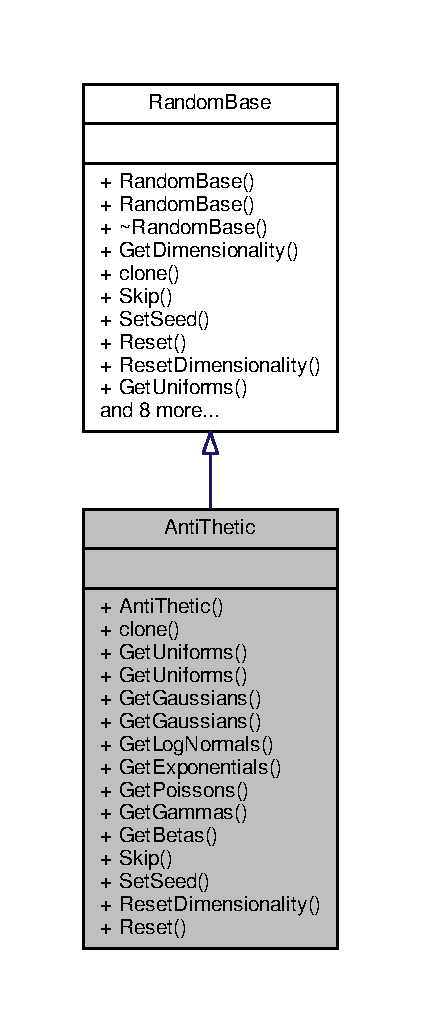
\includegraphics[width=202pt]{classAntiThetic__inherit__graph}
\end{center}
\end{figure}


Collaboration diagram for Anti\+Thetic\+:
\nopagebreak
\begin{figure}[H]
\begin{center}
\leavevmode
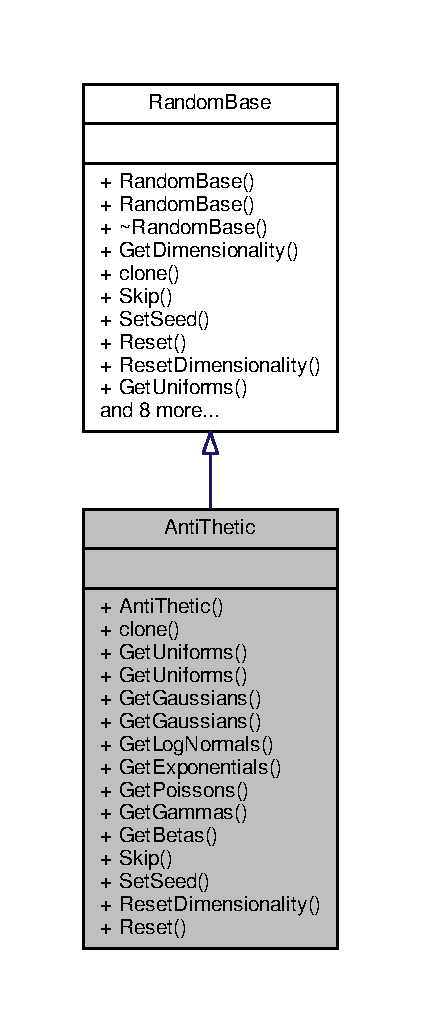
\includegraphics[width=202pt]{classAntiThetic__coll__graph}
\end{center}
\end{figure}
\subsection*{Public Member Functions}
\begin{DoxyCompactItemize}
\item 
\hyperlink{classAntiThetic_aa79b36bdd2f341f5ad2b41f141950044}{Anti\+Thetic} (const \hyperlink{classWrapper}{Wrapper}$<$ \hyperlink{classRandomBase}{Random\+Base} $>$ \&inner\+Generator)
\item 
virtual \hyperlink{classRandomBase}{Random\+Base} $\ast$ \hyperlink{classAntiThetic_ab736855d3978fdc1ff914239cfc51a9d}{clone} () const
\item 
virtual void \hyperlink{classAntiThetic_affc5dff1f5783cb68f3933dd7b25c83a}{Get\+Uniforms} (\hyperlink{classMJArray}{M\+J\+Array} \&variates)
\item 
virtual void \hyperlink{classAntiThetic_a189ea07e81121c1ae4f3c655ec405487}{Get\+Uniforms} (std\+::vector$<$ double $>$ \&variates, double a=0.\+0, double b=1.\+0)
\item 
virtual void \hyperlink{classAntiThetic_ac680e938752f4d5b2a5ba51f5d4862e2}{Get\+Gaussians} (\hyperlink{classMJArray}{M\+J\+Array} \&variates)
\item 
virtual void \hyperlink{classAntiThetic_a82340ce519d6dbdf75f6270193eea703}{Get\+Gaussians} (std\+::vector$<$ double $>$ \&variates, double m=0.\+0, double s=1.\+0)
\item 
virtual void \hyperlink{classAntiThetic_ad14fda6b35f6370d744d0ea53d5b80ba}{Get\+Log\+Normals} (double m, double s, \hyperlink{classMJArray}{M\+J\+Array} \&variates)
\item 
virtual void \hyperlink{classAntiThetic_aa4ee18288564b74c7a2d7e5015e87d6c}{Get\+Exponentials} (double lambda, \hyperlink{classMJArray}{M\+J\+Array} \&variates)
\item 
virtual void \hyperlink{classAntiThetic_af37fd70c21d1d4bf65a0494a4a8c5459}{Get\+Poissons} (double lambda, \hyperlink{classMJArray}{M\+J\+Array} \&variates)
\item 
virtual void \hyperlink{classAntiThetic_a367486230368c4624cabf6172b97dafe}{Get\+Gammas} (double alpha, double beta, \hyperlink{classMJArray}{M\+J\+Array} \&variates)
\item 
virtual void \hyperlink{classAntiThetic_a84fc41c2b4e5a1de78f3399e21c067f8}{Get\+Betas} (double alpha, double beta, \hyperlink{classMJArray}{M\+J\+Array} \&variates)
\item 
virtual void \hyperlink{classAntiThetic_ab401f6a7ce58643b3f147886d837e097}{Skip} (unsigned long number\+Of\+Paths)
\item 
virtual void \hyperlink{classAntiThetic_a0561b133af3db59319d7ede6a52fb1d4}{Set\+Seed} (unsigned long Seed)
\item 
virtual void \hyperlink{classAntiThetic_afb5d6c15a5729be709d905d81582e1b7}{Reset\+Dimensionality} (unsigned long New\+Dimensionality)
\item 
virtual void \hyperlink{classAntiThetic_a54f6452f0017f86580b7af9dfa0172e4}{Reset} ()
\end{DoxyCompactItemize}


\subsection{Constructor \& Destructor Documentation}
\hypertarget{classAntiThetic_aa79b36bdd2f341f5ad2b41f141950044}{}\label{classAntiThetic_aa79b36bdd2f341f5ad2b41f141950044} 
\index{Anti\+Thetic@{Anti\+Thetic}!Anti\+Thetic@{Anti\+Thetic}}
\index{Anti\+Thetic@{Anti\+Thetic}!Anti\+Thetic@{Anti\+Thetic}}
\subsubsection{\texorpdfstring{Anti\+Thetic()}{AntiThetic()}}
{\footnotesize\ttfamily Anti\+Thetic\+::\+Anti\+Thetic (\begin{DoxyParamCaption}\item[{const \hyperlink{classWrapper}{Wrapper}$<$ \hyperlink{classRandomBase}{Random\+Base} $>$ \&}]{inner\+Generator }\end{DoxyParamCaption})}



\subsection{Member Function Documentation}
\hypertarget{classAntiThetic_ab736855d3978fdc1ff914239cfc51a9d}{}\label{classAntiThetic_ab736855d3978fdc1ff914239cfc51a9d} 
\index{Anti\+Thetic@{Anti\+Thetic}!clone@{clone}}
\index{clone@{clone}!Anti\+Thetic@{Anti\+Thetic}}
\subsubsection{\texorpdfstring{clone()}{clone()}}
{\footnotesize\ttfamily virtual \hyperlink{classRandomBase}{Random\+Base}$\ast$ Anti\+Thetic\+::clone (\begin{DoxyParamCaption}{ }\end{DoxyParamCaption}) const\hspace{0.3cm}{\ttfamily [virtual]}}



Implements \hyperlink{classRandomBase_a0906f4590283535ec40427ad31ba7850}{Random\+Base}.

\hypertarget{classAntiThetic_a84fc41c2b4e5a1de78f3399e21c067f8}{}\label{classAntiThetic_a84fc41c2b4e5a1de78f3399e21c067f8} 
\index{Anti\+Thetic@{Anti\+Thetic}!Get\+Betas@{Get\+Betas}}
\index{Get\+Betas@{Get\+Betas}!Anti\+Thetic@{Anti\+Thetic}}
\subsubsection{\texorpdfstring{Get\+Betas()}{GetBetas()}}
{\footnotesize\ttfamily virtual void Anti\+Thetic\+::\+Get\+Betas (\begin{DoxyParamCaption}\item[{double}]{alpha,  }\item[{double}]{beta,  }\item[{\hyperlink{classMJArray}{M\+J\+Array} \&}]{variates }\end{DoxyParamCaption})\hspace{0.3cm}{\ttfamily [virtual]}}



Reimplemented from \hyperlink{classRandomBase_aa3f3efa1333ab5d7689b8cc7ebd26622}{Random\+Base}.

\hypertarget{classAntiThetic_aa4ee18288564b74c7a2d7e5015e87d6c}{}\label{classAntiThetic_aa4ee18288564b74c7a2d7e5015e87d6c} 
\index{Anti\+Thetic@{Anti\+Thetic}!Get\+Exponentials@{Get\+Exponentials}}
\index{Get\+Exponentials@{Get\+Exponentials}!Anti\+Thetic@{Anti\+Thetic}}
\subsubsection{\texorpdfstring{Get\+Exponentials()}{GetExponentials()}}
{\footnotesize\ttfamily virtual void Anti\+Thetic\+::\+Get\+Exponentials (\begin{DoxyParamCaption}\item[{double}]{lambda,  }\item[{\hyperlink{classMJArray}{M\+J\+Array} \&}]{variates }\end{DoxyParamCaption})\hspace{0.3cm}{\ttfamily [virtual]}}



Reimplemented from \hyperlink{classRandomBase_ad1d2c39a8440f67cffda3ad41a4f9975}{Random\+Base}.

\hypertarget{classAntiThetic_a367486230368c4624cabf6172b97dafe}{}\label{classAntiThetic_a367486230368c4624cabf6172b97dafe} 
\index{Anti\+Thetic@{Anti\+Thetic}!Get\+Gammas@{Get\+Gammas}}
\index{Get\+Gammas@{Get\+Gammas}!Anti\+Thetic@{Anti\+Thetic}}
\subsubsection{\texorpdfstring{Get\+Gammas()}{GetGammas()}}
{\footnotesize\ttfamily virtual void Anti\+Thetic\+::\+Get\+Gammas (\begin{DoxyParamCaption}\item[{double}]{alpha,  }\item[{double}]{beta,  }\item[{\hyperlink{classMJArray}{M\+J\+Array} \&}]{variates }\end{DoxyParamCaption})\hspace{0.3cm}{\ttfamily [virtual]}}



Reimplemented from \hyperlink{classRandomBase_a5b5c89afe295ba49a5474cdc3bf80c3d}{Random\+Base}.

\hypertarget{classAntiThetic_ac680e938752f4d5b2a5ba51f5d4862e2}{}\label{classAntiThetic_ac680e938752f4d5b2a5ba51f5d4862e2} 
\index{Anti\+Thetic@{Anti\+Thetic}!Get\+Gaussians@{Get\+Gaussians}}
\index{Get\+Gaussians@{Get\+Gaussians}!Anti\+Thetic@{Anti\+Thetic}}
\subsubsection{\texorpdfstring{Get\+Gaussians()}{GetGaussians()}\hspace{0.1cm}{\footnotesize\ttfamily [1/2]}}
{\footnotesize\ttfamily virtual void Anti\+Thetic\+::\+Get\+Gaussians (\begin{DoxyParamCaption}\item[{\hyperlink{classMJArray}{M\+J\+Array} \&}]{variates }\end{DoxyParamCaption})\hspace{0.3cm}{\ttfamily [virtual]}}



Reimplemented from \hyperlink{classRandomBase_aac297a1b64959492831f5e9a1f28c03d}{Random\+Base}.

\hypertarget{classAntiThetic_a82340ce519d6dbdf75f6270193eea703}{}\label{classAntiThetic_a82340ce519d6dbdf75f6270193eea703} 
\index{Anti\+Thetic@{Anti\+Thetic}!Get\+Gaussians@{Get\+Gaussians}}
\index{Get\+Gaussians@{Get\+Gaussians}!Anti\+Thetic@{Anti\+Thetic}}
\subsubsection{\texorpdfstring{Get\+Gaussians()}{GetGaussians()}\hspace{0.1cm}{\footnotesize\ttfamily [2/2]}}
{\footnotesize\ttfamily virtual void Anti\+Thetic\+::\+Get\+Gaussians (\begin{DoxyParamCaption}\item[{std\+::vector$<$ double $>$ \&}]{variates,  }\item[{double}]{m = {\ttfamily 0.0},  }\item[{double}]{s = {\ttfamily 1.0} }\end{DoxyParamCaption})\hspace{0.3cm}{\ttfamily [virtual]}}



Reimplemented from \hyperlink{classRandomBase_a8428b19f897b202363c12df1471a8d52}{Random\+Base}.

\hypertarget{classAntiThetic_ad14fda6b35f6370d744d0ea53d5b80ba}{}\label{classAntiThetic_ad14fda6b35f6370d744d0ea53d5b80ba} 
\index{Anti\+Thetic@{Anti\+Thetic}!Get\+Log\+Normals@{Get\+Log\+Normals}}
\index{Get\+Log\+Normals@{Get\+Log\+Normals}!Anti\+Thetic@{Anti\+Thetic}}
\subsubsection{\texorpdfstring{Get\+Log\+Normals()}{GetLogNormals()}}
{\footnotesize\ttfamily virtual void Anti\+Thetic\+::\+Get\+Log\+Normals (\begin{DoxyParamCaption}\item[{double}]{m,  }\item[{double}]{s,  }\item[{\hyperlink{classMJArray}{M\+J\+Array} \&}]{variates }\end{DoxyParamCaption})\hspace{0.3cm}{\ttfamily [virtual]}}



Reimplemented from \hyperlink{classRandomBase_a734f1712b1179fb31380e04da4a27f20}{Random\+Base}.

\hypertarget{classAntiThetic_af37fd70c21d1d4bf65a0494a4a8c5459}{}\label{classAntiThetic_af37fd70c21d1d4bf65a0494a4a8c5459} 
\index{Anti\+Thetic@{Anti\+Thetic}!Get\+Poissons@{Get\+Poissons}}
\index{Get\+Poissons@{Get\+Poissons}!Anti\+Thetic@{Anti\+Thetic}}
\subsubsection{\texorpdfstring{Get\+Poissons()}{GetPoissons()}}
{\footnotesize\ttfamily virtual void Anti\+Thetic\+::\+Get\+Poissons (\begin{DoxyParamCaption}\item[{double}]{lambda,  }\item[{\hyperlink{classMJArray}{M\+J\+Array} \&}]{variates }\end{DoxyParamCaption})\hspace{0.3cm}{\ttfamily [virtual]}}



Reimplemented from \hyperlink{classRandomBase_aa2e79f1f4c55c36df9c701d29e9b08a5}{Random\+Base}.

\hypertarget{classAntiThetic_affc5dff1f5783cb68f3933dd7b25c83a}{}\label{classAntiThetic_affc5dff1f5783cb68f3933dd7b25c83a} 
\index{Anti\+Thetic@{Anti\+Thetic}!Get\+Uniforms@{Get\+Uniforms}}
\index{Get\+Uniforms@{Get\+Uniforms}!Anti\+Thetic@{Anti\+Thetic}}
\subsubsection{\texorpdfstring{Get\+Uniforms()}{GetUniforms()}\hspace{0.1cm}{\footnotesize\ttfamily [1/2]}}
{\footnotesize\ttfamily virtual void Anti\+Thetic\+::\+Get\+Uniforms (\begin{DoxyParamCaption}\item[{\hyperlink{classMJArray}{M\+J\+Array} \&}]{variates }\end{DoxyParamCaption})\hspace{0.3cm}{\ttfamily [virtual]}}



Implements \hyperlink{classRandomBase_aa061fb77f53969f6fbe40c7454c69eb9}{Random\+Base}.

\hypertarget{classAntiThetic_a189ea07e81121c1ae4f3c655ec405487}{}\label{classAntiThetic_a189ea07e81121c1ae4f3c655ec405487} 
\index{Anti\+Thetic@{Anti\+Thetic}!Get\+Uniforms@{Get\+Uniforms}}
\index{Get\+Uniforms@{Get\+Uniforms}!Anti\+Thetic@{Anti\+Thetic}}
\subsubsection{\texorpdfstring{Get\+Uniforms()}{GetUniforms()}\hspace{0.1cm}{\footnotesize\ttfamily [2/2]}}
{\footnotesize\ttfamily virtual void Anti\+Thetic\+::\+Get\+Uniforms (\begin{DoxyParamCaption}\item[{std\+::vector$<$ double $>$ \&}]{variates,  }\item[{double}]{a = {\ttfamily 0.0},  }\item[{double}]{b = {\ttfamily 1.0} }\end{DoxyParamCaption})\hspace{0.3cm}{\ttfamily [virtual]}}



Implements \hyperlink{classRandomBase_a3bbf85695dbb1a9462a2b6c3f10af969}{Random\+Base}.

\hypertarget{classAntiThetic_a54f6452f0017f86580b7af9dfa0172e4}{}\label{classAntiThetic_a54f6452f0017f86580b7af9dfa0172e4} 
\index{Anti\+Thetic@{Anti\+Thetic}!Reset@{Reset}}
\index{Reset@{Reset}!Anti\+Thetic@{Anti\+Thetic}}
\subsubsection{\texorpdfstring{Reset()}{Reset()}}
{\footnotesize\ttfamily virtual void Anti\+Thetic\+::\+Reset (\begin{DoxyParamCaption}{ }\end{DoxyParamCaption})\hspace{0.3cm}{\ttfamily [virtual]}}



Implements \hyperlink{classRandomBase_a6e35c1467b37fc8c5e262297223685eb}{Random\+Base}.

\hypertarget{classAntiThetic_afb5d6c15a5729be709d905d81582e1b7}{}\label{classAntiThetic_afb5d6c15a5729be709d905d81582e1b7} 
\index{Anti\+Thetic@{Anti\+Thetic}!Reset\+Dimensionality@{Reset\+Dimensionality}}
\index{Reset\+Dimensionality@{Reset\+Dimensionality}!Anti\+Thetic@{Anti\+Thetic}}
\subsubsection{\texorpdfstring{Reset\+Dimensionality()}{ResetDimensionality()}}
{\footnotesize\ttfamily virtual void Anti\+Thetic\+::\+Reset\+Dimensionality (\begin{DoxyParamCaption}\item[{unsigned long}]{New\+Dimensionality }\end{DoxyParamCaption})\hspace{0.3cm}{\ttfamily [virtual]}}



Reimplemented from \hyperlink{classRandomBase_a8931e429ae130ea44af5469dc6ae728f}{Random\+Base}.

\hypertarget{classAntiThetic_a0561b133af3db59319d7ede6a52fb1d4}{}\label{classAntiThetic_a0561b133af3db59319d7ede6a52fb1d4} 
\index{Anti\+Thetic@{Anti\+Thetic}!Set\+Seed@{Set\+Seed}}
\index{Set\+Seed@{Set\+Seed}!Anti\+Thetic@{Anti\+Thetic}}
\subsubsection{\texorpdfstring{Set\+Seed()}{SetSeed()}}
{\footnotesize\ttfamily virtual void Anti\+Thetic\+::\+Set\+Seed (\begin{DoxyParamCaption}\item[{unsigned long}]{Seed }\end{DoxyParamCaption})\hspace{0.3cm}{\ttfamily [virtual]}}



Implements \hyperlink{classRandomBase_ae93f26c38d1675ef07cb1fd29b894b26}{Random\+Base}.

\hypertarget{classAntiThetic_ab401f6a7ce58643b3f147886d837e097}{}\label{classAntiThetic_ab401f6a7ce58643b3f147886d837e097} 
\index{Anti\+Thetic@{Anti\+Thetic}!Skip@{Skip}}
\index{Skip@{Skip}!Anti\+Thetic@{Anti\+Thetic}}
\subsubsection{\texorpdfstring{Skip()}{Skip()}}
{\footnotesize\ttfamily virtual void Anti\+Thetic\+::\+Skip (\begin{DoxyParamCaption}\item[{unsigned long}]{number\+Of\+Paths }\end{DoxyParamCaption})\hspace{0.3cm}{\ttfamily [virtual]}}



Implements \hyperlink{classRandomBase_a0531f44e3e2a71d14ef1490aa5d90b77}{Random\+Base}.



The documentation for this class was generated from the following file\+:\begin{DoxyCompactItemize}
\item 
\hyperlink{AntiThetic_8h}{Anti\+Thetic.\+h}\end{DoxyCompactItemize}

\hypertarget{classxlw_1_1ArgListFactory}{}\section{xlw\+:\+:Arg\+List\+Factory$<$ T $>$ Class Template Reference}
\label{classxlw_1_1ArgListFactory}\index{xlw\+::\+Arg\+List\+Factory$<$ T $>$@{xlw\+::\+Arg\+List\+Factory$<$ T $>$}}


{\ttfamily \#include $<$Arg\+List\+Factory.\+h$>$}



Inheritance diagram for xlw\+:\+:Arg\+List\+Factory$<$ T $>$\+:
\nopagebreak
\begin{figure}[H]
\begin{center}
\leavevmode
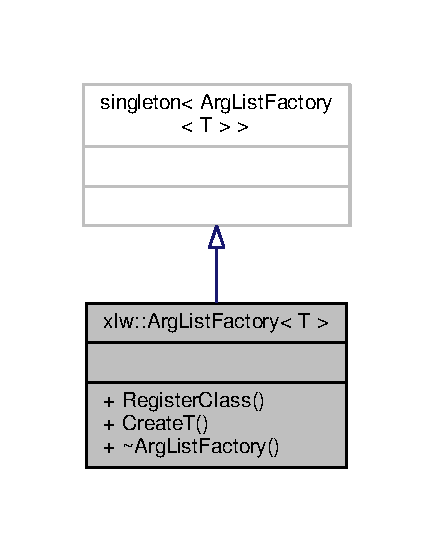
\includegraphics[width=208pt]{classxlw_1_1ArgListFactory__inherit__graph}
\end{center}
\end{figure}


Collaboration diagram for xlw\+:\+:Arg\+List\+Factory$<$ T $>$\+:
\nopagebreak
\begin{figure}[H]
\begin{center}
\leavevmode
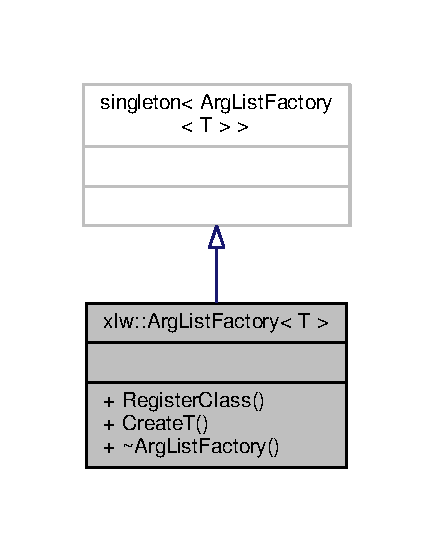
\includegraphics[width=208pt]{classxlw_1_1ArgListFactory__coll__graph}
\end{center}
\end{figure}
\subsection*{Public Types}
\begin{DoxyCompactItemize}
\item 
typedef T $\ast$($\ast$ \hyperlink{classxlw_1_1ArgListFactory_a2bd565ada3ddbebcec91aea216f90e22}{Create\+T\+Function}) (const Argument\+List \&)
\end{DoxyCompactItemize}
\subsection*{Public Member Functions}
\begin{DoxyCompactItemize}
\item 
void \hyperlink{classxlw_1_1ArgListFactory_a5d81eab40e16198ecf994f6404792550}{Register\+Class} (std\+::string Class\+Id, \hyperlink{classxlw_1_1ArgListFactory_a2bd565ada3ddbebcec91aea216f90e22}{Create\+T\+Function})
\item 
T $\ast$ \hyperlink{classxlw_1_1ArgListFactory_a42e5fdbde035d3ab8bd383a0f32bc35f}{CreateT} (Argument\+List \hyperlink{path__generation_8h_a75c13cde2074f502cc4348c70528572d}{args})
\item 
\hyperlink{classxlw_1_1ArgListFactory_a5f919feedf0ee38addb2ad97a20c9c50}{$\sim$\+Arg\+List\+Factory} ()
\end{DoxyCompactItemize}


\subsection{Member Typedef Documentation}
\hypertarget{classxlw_1_1ArgListFactory_a2bd565ada3ddbebcec91aea216f90e22}{}\label{classxlw_1_1ArgListFactory_a2bd565ada3ddbebcec91aea216f90e22} 
\index{xlw\+::\+Arg\+List\+Factory@{xlw\+::\+Arg\+List\+Factory}!Create\+T\+Function@{Create\+T\+Function}}
\index{Create\+T\+Function@{Create\+T\+Function}!xlw\+::\+Arg\+List\+Factory@{xlw\+::\+Arg\+List\+Factory}}
\subsubsection{\texorpdfstring{Create\+T\+Function}{CreateTFunction}}
{\footnotesize\ttfamily template$<$typename T $>$ \\
typedef T$\ast$($\ast$ \hyperlink{classxlw_1_1ArgListFactory}{xlw\+::\+Arg\+List\+Factory}$<$ T $>$\+::Create\+T\+Function) (const Argument\+List \&)}



\subsection{Constructor \& Destructor Documentation}
\hypertarget{classxlw_1_1ArgListFactory_a5f919feedf0ee38addb2ad97a20c9c50}{}\label{classxlw_1_1ArgListFactory_a5f919feedf0ee38addb2ad97a20c9c50} 
\index{xlw\+::\+Arg\+List\+Factory@{xlw\+::\+Arg\+List\+Factory}!````~Arg\+List\+Factory@{$\sim$\+Arg\+List\+Factory}}
\index{````~Arg\+List\+Factory@{$\sim$\+Arg\+List\+Factory}!xlw\+::\+Arg\+List\+Factory@{xlw\+::\+Arg\+List\+Factory}}
\subsubsection{\texorpdfstring{$\sim$\+Arg\+List\+Factory()}{~ArgListFactory()}}
{\footnotesize\ttfamily template$<$typename T $>$ \\
\hyperlink{classxlw_1_1ArgListFactory}{xlw\+::\+Arg\+List\+Factory}$<$ T $>$\+::$\sim$\hyperlink{classxlw_1_1ArgListFactory}{Arg\+List\+Factory} (\begin{DoxyParamCaption}{ }\end{DoxyParamCaption})\hspace{0.3cm}{\ttfamily [inline]}}



\subsection{Member Function Documentation}
\hypertarget{classxlw_1_1ArgListFactory_a42e5fdbde035d3ab8bd383a0f32bc35f}{}\label{classxlw_1_1ArgListFactory_a42e5fdbde035d3ab8bd383a0f32bc35f} 
\index{xlw\+::\+Arg\+List\+Factory@{xlw\+::\+Arg\+List\+Factory}!CreateT@{CreateT}}
\index{CreateT@{CreateT}!xlw\+::\+Arg\+List\+Factory@{xlw\+::\+Arg\+List\+Factory}}
\subsubsection{\texorpdfstring{Create\+T()}{CreateT()}}
{\footnotesize\ttfamily template$<$typename T $>$ \\
T $\ast$ \hyperlink{classxlw_1_1ArgListFactory}{xlw\+::\+Arg\+List\+Factory}$<$ T $>$\+::CreateT (\begin{DoxyParamCaption}\item[{Argument\+List}]{args }\end{DoxyParamCaption})}

\hypertarget{classxlw_1_1ArgListFactory_a5d81eab40e16198ecf994f6404792550}{}\label{classxlw_1_1ArgListFactory_a5d81eab40e16198ecf994f6404792550} 
\index{xlw\+::\+Arg\+List\+Factory@{xlw\+::\+Arg\+List\+Factory}!Register\+Class@{Register\+Class}}
\index{Register\+Class@{Register\+Class}!xlw\+::\+Arg\+List\+Factory@{xlw\+::\+Arg\+List\+Factory}}
\subsubsection{\texorpdfstring{Register\+Class()}{RegisterClass()}}
{\footnotesize\ttfamily template$<$typename T $>$ \\
void \hyperlink{classxlw_1_1ArgListFactory}{xlw\+::\+Arg\+List\+Factory}$<$ T $>$\+::Register\+Class (\begin{DoxyParamCaption}\item[{std\+::string}]{Class\+Id,  }\item[{\hyperlink{classxlw_1_1ArgListFactory_a2bd565ada3ddbebcec91aea216f90e22}{Create\+T\+Function}}]{Creator\+Function }\end{DoxyParamCaption})}



The documentation for this class was generated from the following file\+:\begin{DoxyCompactItemize}
\item 
\hyperlink{ArgListFactory_8h}{Arg\+List\+Factory.\+h}\end{DoxyCompactItemize}

\hypertarget{classBinomialTree}{}\section{Binomial\+Tree Class Reference}
\label{classBinomialTree}\index{Binomial\+Tree@{Binomial\+Tree}}


{\ttfamily \#include $<$Binomial\+Tree\+Linear.\+h$>$}



Collaboration diagram for Binomial\+Tree\+:
\nopagebreak
\begin{figure}[H]
\begin{center}
\leavevmode
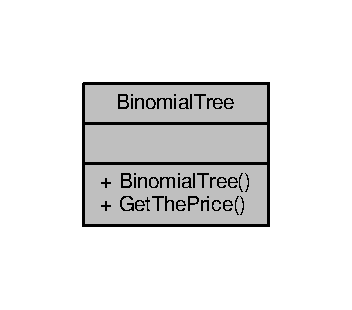
\includegraphics[width=169pt]{classBinomialTree__coll__graph}
\end{center}
\end{figure}
\subsection*{Public Member Functions}
\begin{DoxyCompactItemize}
\item 
\hyperlink{classBinomialTree_a2eb5a7209e8d41936ae4b00a007b7641}{Binomial\+Tree} (double Spot\+\_\+, const \hyperlink{classParameters}{Parameters} \&r\+\_\+, const \hyperlink{classParameters}{Parameters} \&d\+\_\+, double Volatility\+\_\+, unsigned long Steps, double Time)
\item 
double \hyperlink{classBinomialTree_a07abae93043bcd34d7144913b2290b03}{Get\+The\+Price} (\hyperlink{classTreeProduct}{Tree\+Product} \&The\+Product)
\end{DoxyCompactItemize}


\subsection{Constructor \& Destructor Documentation}
\hypertarget{classBinomialTree_a2eb5a7209e8d41936ae4b00a007b7641}{}\label{classBinomialTree_a2eb5a7209e8d41936ae4b00a007b7641} 
\index{Binomial\+Tree@{Binomial\+Tree}!Binomial\+Tree@{Binomial\+Tree}}
\index{Binomial\+Tree@{Binomial\+Tree}!Binomial\+Tree@{Binomial\+Tree}}
\subsubsection{\texorpdfstring{Binomial\+Tree()}{BinomialTree()}}
{\footnotesize\ttfamily Binomial\+Tree\+::\+Binomial\+Tree (\begin{DoxyParamCaption}\item[{double}]{Spot\+\_\+,  }\item[{const \hyperlink{classParameters}{Parameters} \&}]{r\+\_\+,  }\item[{const \hyperlink{classParameters}{Parameters} \&}]{d\+\_\+,  }\item[{double}]{Volatility\+\_\+,  }\item[{unsigned long}]{Steps,  }\item[{double}]{Time }\end{DoxyParamCaption})}



\subsection{Member Function Documentation}
\hypertarget{classBinomialTree_a07abae93043bcd34d7144913b2290b03}{}\label{classBinomialTree_a07abae93043bcd34d7144913b2290b03} 
\index{Binomial\+Tree@{Binomial\+Tree}!Get\+The\+Price@{Get\+The\+Price}}
\index{Get\+The\+Price@{Get\+The\+Price}!Binomial\+Tree@{Binomial\+Tree}}
\subsubsection{\texorpdfstring{Get\+The\+Price()}{GetThePrice()}}
{\footnotesize\ttfamily double Binomial\+Tree\+::\+Get\+The\+Price (\begin{DoxyParamCaption}\item[{\hyperlink{classTreeProduct}{Tree\+Product} \&}]{The\+Product }\end{DoxyParamCaption})}



The documentation for this class was generated from the following file\+:\begin{DoxyCompactItemize}
\item 
\hyperlink{BinomialTreeLinear_8h}{Binomial\+Tree\+Linear.\+h}\end{DoxyCompactItemize}

\hypertarget{classBinomialTreeAmericanBarrier}{}\section{Binomial\+Tree\+American\+Barrier Class Reference}
\label{classBinomialTreeAmericanBarrier}\index{Binomial\+Tree\+American\+Barrier@{Binomial\+Tree\+American\+Barrier}}


{\ttfamily \#include $<$Binomial\+Tree\+American\+Barrier.\+h$>$}



Collaboration diagram for Binomial\+Tree\+American\+Barrier\+:
\nopagebreak
\begin{figure}[H]
\begin{center}
\leavevmode
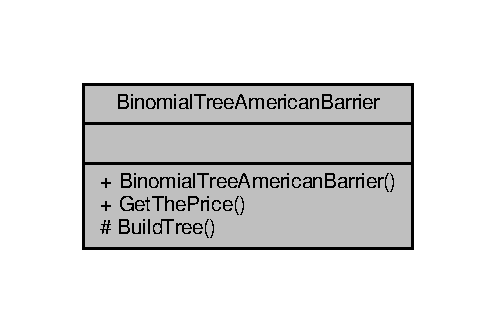
\includegraphics[width=238pt]{classBinomialTreeAmericanBarrier__coll__graph}
\end{center}
\end{figure}
\subsection*{Public Member Functions}
\begin{DoxyCompactItemize}
\item 
\hyperlink{classBinomialTreeAmericanBarrier_aa02aa598a64b7372957117d92f037977}{Binomial\+Tree\+American\+Barrier} (double Spot\+\_\+, const \hyperlink{classParameters}{Parameters} \&r\+\_\+, const \hyperlink{classParameters}{Parameters} \&d\+\_\+, double Volatility\+\_\+, unsigned long Steps, double Time)
\item 
double \hyperlink{classBinomialTreeAmericanBarrier_a6119001ee5107dbd5e19881a47e22fdd}{Get\+The\+Price} (const \hyperlink{classTreeProduct}{Tree\+Product} \&The\+Product)
\end{DoxyCompactItemize}
\subsection*{Protected Member Functions}
\begin{DoxyCompactItemize}
\item 
void \hyperlink{classBinomialTreeAmericanBarrier_adaae6378697610ce4f9bc2be3912aed6}{Build\+Tree} ()
\end{DoxyCompactItemize}


\subsection{Constructor \& Destructor Documentation}
\hypertarget{classBinomialTreeAmericanBarrier_aa02aa598a64b7372957117d92f037977}{}\label{classBinomialTreeAmericanBarrier_aa02aa598a64b7372957117d92f037977} 
\index{Binomial\+Tree\+American\+Barrier@{Binomial\+Tree\+American\+Barrier}!Binomial\+Tree\+American\+Barrier@{Binomial\+Tree\+American\+Barrier}}
\index{Binomial\+Tree\+American\+Barrier@{Binomial\+Tree\+American\+Barrier}!Binomial\+Tree\+American\+Barrier@{Binomial\+Tree\+American\+Barrier}}
\subsubsection{\texorpdfstring{Binomial\+Tree\+American\+Barrier()}{BinomialTreeAmericanBarrier()}}
{\footnotesize\ttfamily Binomial\+Tree\+American\+Barrier\+::\+Binomial\+Tree\+American\+Barrier (\begin{DoxyParamCaption}\item[{double}]{Spot\+\_\+,  }\item[{const \hyperlink{classParameters}{Parameters} \&}]{r\+\_\+,  }\item[{const \hyperlink{classParameters}{Parameters} \&}]{d\+\_\+,  }\item[{double}]{Volatility\+\_\+,  }\item[{unsigned long}]{Steps,  }\item[{double}]{Time }\end{DoxyParamCaption})}



\subsection{Member Function Documentation}
\hypertarget{classBinomialTreeAmericanBarrier_adaae6378697610ce4f9bc2be3912aed6}{}\label{classBinomialTreeAmericanBarrier_adaae6378697610ce4f9bc2be3912aed6} 
\index{Binomial\+Tree\+American\+Barrier@{Binomial\+Tree\+American\+Barrier}!Build\+Tree@{Build\+Tree}}
\index{Build\+Tree@{Build\+Tree}!Binomial\+Tree\+American\+Barrier@{Binomial\+Tree\+American\+Barrier}}
\subsubsection{\texorpdfstring{Build\+Tree()}{BuildTree()}}
{\footnotesize\ttfamily void Binomial\+Tree\+American\+Barrier\+::\+Build\+Tree (\begin{DoxyParamCaption}{ }\end{DoxyParamCaption})\hspace{0.3cm}{\ttfamily [protected]}}

\hypertarget{classBinomialTreeAmericanBarrier_a6119001ee5107dbd5e19881a47e22fdd}{}\label{classBinomialTreeAmericanBarrier_a6119001ee5107dbd5e19881a47e22fdd} 
\index{Binomial\+Tree\+American\+Barrier@{Binomial\+Tree\+American\+Barrier}!Get\+The\+Price@{Get\+The\+Price}}
\index{Get\+The\+Price@{Get\+The\+Price}!Binomial\+Tree\+American\+Barrier@{Binomial\+Tree\+American\+Barrier}}
\subsubsection{\texorpdfstring{Get\+The\+Price()}{GetThePrice()}}
{\footnotesize\ttfamily double Binomial\+Tree\+American\+Barrier\+::\+Get\+The\+Price (\begin{DoxyParamCaption}\item[{const \hyperlink{classTreeProduct}{Tree\+Product} \&}]{The\+Product }\end{DoxyParamCaption})}



The documentation for this class was generated from the following file\+:\begin{DoxyCompactItemize}
\item 
\hyperlink{BinomialTreeAmericanBarrier_8h}{Binomial\+Tree\+American\+Barrier.\+h}\end{DoxyCompactItemize}

\hypertarget{classBinomialTreeMartingale}{}\section{Binomial\+Tree\+Martingale Class Reference}
\label{classBinomialTreeMartingale}\index{Binomial\+Tree\+Martingale@{Binomial\+Tree\+Martingale}}


{\ttfamily \#include $<$Binomial\+Tree\+Martingale.\+h$>$}



Collaboration diagram for Binomial\+Tree\+Martingale\+:
\nopagebreak
\begin{figure}[H]
\begin{center}
\leavevmode
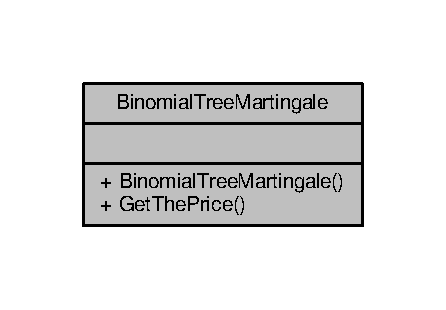
\includegraphics[width=214pt]{classBinomialTreeMartingale__coll__graph}
\end{center}
\end{figure}
\subsection*{Public Member Functions}
\begin{DoxyCompactItemize}
\item 
\hyperlink{classBinomialTreeMartingale_a3d478aeaa74ebbdde22d699cce66eaf4}{Binomial\+Tree\+Martingale} (double Spot\+\_\+, double Strike\+\_\+, const \hyperlink{classParameters}{Parameters} \&r\+\_\+, const \hyperlink{classParameters}{Parameters} \&d\+\_\+, double Volatility\+\_\+, unsigned long Steps, double Time)
\item 
double \hyperlink{classBinomialTreeMartingale_a9cc63624311a9f63664fd08aa78533f9}{Get\+The\+Price} (const \hyperlink{classTreeProduct}{Tree\+Product} \&The\+Product, unsigned long Steps)
\end{DoxyCompactItemize}


\subsection{Constructor \& Destructor Documentation}
\hypertarget{classBinomialTreeMartingale_a3d478aeaa74ebbdde22d699cce66eaf4}{}\label{classBinomialTreeMartingale_a3d478aeaa74ebbdde22d699cce66eaf4} 
\index{Binomial\+Tree\+Martingale@{Binomial\+Tree\+Martingale}!Binomial\+Tree\+Martingale@{Binomial\+Tree\+Martingale}}
\index{Binomial\+Tree\+Martingale@{Binomial\+Tree\+Martingale}!Binomial\+Tree\+Martingale@{Binomial\+Tree\+Martingale}}
\subsubsection{\texorpdfstring{Binomial\+Tree\+Martingale()}{BinomialTreeMartingale()}}
{\footnotesize\ttfamily Binomial\+Tree\+Martingale\+::\+Binomial\+Tree\+Martingale (\begin{DoxyParamCaption}\item[{double}]{Spot\+\_\+,  }\item[{double}]{Strike\+\_\+,  }\item[{const \hyperlink{classParameters}{Parameters} \&}]{r\+\_\+,  }\item[{const \hyperlink{classParameters}{Parameters} \&}]{d\+\_\+,  }\item[{double}]{Volatility\+\_\+,  }\item[{unsigned long}]{Steps,  }\item[{double}]{Time }\end{DoxyParamCaption})}



\subsection{Member Function Documentation}
\hypertarget{classBinomialTreeMartingale_a9cc63624311a9f63664fd08aa78533f9}{}\label{classBinomialTreeMartingale_a9cc63624311a9f63664fd08aa78533f9} 
\index{Binomial\+Tree\+Martingale@{Binomial\+Tree\+Martingale}!Get\+The\+Price@{Get\+The\+Price}}
\index{Get\+The\+Price@{Get\+The\+Price}!Binomial\+Tree\+Martingale@{Binomial\+Tree\+Martingale}}
\subsubsection{\texorpdfstring{Get\+The\+Price()}{GetThePrice()}}
{\footnotesize\ttfamily double Binomial\+Tree\+Martingale\+::\+Get\+The\+Price (\begin{DoxyParamCaption}\item[{const \hyperlink{classTreeProduct}{Tree\+Product} \&}]{The\+Product,  }\item[{unsigned long}]{Steps }\end{DoxyParamCaption})}



The documentation for this class was generated from the following file\+:\begin{DoxyCompactItemize}
\item 
\hyperlink{BinomialTreeMartingale_8h}{Binomial\+Tree\+Martingale.\+h}\end{DoxyCompactItemize}

\hypertarget{classBinomialTreeTermStructure}{}\section{Binomial\+Tree\+Term\+Structure Class Reference}
\label{classBinomialTreeTermStructure}\index{Binomial\+Tree\+Term\+Structure@{Binomial\+Tree\+Term\+Structure}}


{\ttfamily \#include $<$Binomial\+Tree\+Term\+Structure.\+h$>$}



Collaboration diagram for Binomial\+Tree\+Term\+Structure\+:
\nopagebreak
\begin{figure}[H]
\begin{center}
\leavevmode
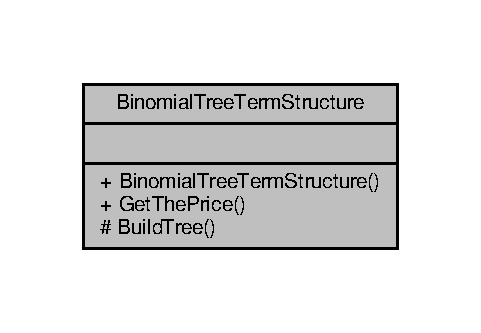
\includegraphics[width=231pt]{classBinomialTreeTermStructure__coll__graph}
\end{center}
\end{figure}
\subsection*{Public Member Functions}
\begin{DoxyCompactItemize}
\item 
\hyperlink{classBinomialTreeTermStructure_a3f364298f038d37e9b239443f0373945}{Binomial\+Tree\+Term\+Structure} (double Spot, const \hyperlink{classParameters}{Parameters} \&r, const \hyperlink{classParameters}{Parameters} \&d, std\+::vector$<$ \hyperlink{structVolatilityTermStructure}{Volatility\+Term\+Structure} $>$ Volatility, unsigned long Steps, double Time)
\item 
double \hyperlink{classBinomialTreeTermStructure_ab328bc5ad38c374992dc1d595e3465c4}{Get\+The\+Price} (const \hyperlink{classTreeProduct}{Tree\+Product} \&The\+Product)
\end{DoxyCompactItemize}
\subsection*{Protected Member Functions}
\begin{DoxyCompactItemize}
\item 
void \hyperlink{classBinomialTreeTermStructure_a7cfa6b6f89f80964a0294ad1d1397254}{Build\+Tree} ()
\end{DoxyCompactItemize}


\subsection{Constructor \& Destructor Documentation}
\hypertarget{classBinomialTreeTermStructure_a3f364298f038d37e9b239443f0373945}{}\label{classBinomialTreeTermStructure_a3f364298f038d37e9b239443f0373945} 
\index{Binomial\+Tree\+Term\+Structure@{Binomial\+Tree\+Term\+Structure}!Binomial\+Tree\+Term\+Structure@{Binomial\+Tree\+Term\+Structure}}
\index{Binomial\+Tree\+Term\+Structure@{Binomial\+Tree\+Term\+Structure}!Binomial\+Tree\+Term\+Structure@{Binomial\+Tree\+Term\+Structure}}
\subsubsection{\texorpdfstring{Binomial\+Tree\+Term\+Structure()}{BinomialTreeTermStructure()}}
{\footnotesize\ttfamily Binomial\+Tree\+Term\+Structure\+::\+Binomial\+Tree\+Term\+Structure (\begin{DoxyParamCaption}\item[{double}]{Spot,  }\item[{const \hyperlink{classParameters}{Parameters} \&}]{r,  }\item[{const \hyperlink{classParameters}{Parameters} \&}]{d,  }\item[{std\+::vector$<$ \hyperlink{structVolatilityTermStructure}{Volatility\+Term\+Structure} $>$}]{Volatility,  }\item[{unsigned long}]{Steps,  }\item[{double}]{Time }\end{DoxyParamCaption})}



\subsection{Member Function Documentation}
\hypertarget{classBinomialTreeTermStructure_a7cfa6b6f89f80964a0294ad1d1397254}{}\label{classBinomialTreeTermStructure_a7cfa6b6f89f80964a0294ad1d1397254} 
\index{Binomial\+Tree\+Term\+Structure@{Binomial\+Tree\+Term\+Structure}!Build\+Tree@{Build\+Tree}}
\index{Build\+Tree@{Build\+Tree}!Binomial\+Tree\+Term\+Structure@{Binomial\+Tree\+Term\+Structure}}
\subsubsection{\texorpdfstring{Build\+Tree()}{BuildTree()}}
{\footnotesize\ttfamily void Binomial\+Tree\+Term\+Structure\+::\+Build\+Tree (\begin{DoxyParamCaption}{ }\end{DoxyParamCaption})\hspace{0.3cm}{\ttfamily [protected]}}

\hypertarget{classBinomialTreeTermStructure_ab328bc5ad38c374992dc1d595e3465c4}{}\label{classBinomialTreeTermStructure_ab328bc5ad38c374992dc1d595e3465c4} 
\index{Binomial\+Tree\+Term\+Structure@{Binomial\+Tree\+Term\+Structure}!Get\+The\+Price@{Get\+The\+Price}}
\index{Get\+The\+Price@{Get\+The\+Price}!Binomial\+Tree\+Term\+Structure@{Binomial\+Tree\+Term\+Structure}}
\subsubsection{\texorpdfstring{Get\+The\+Price()}{GetThePrice()}}
{\footnotesize\ttfamily double Binomial\+Tree\+Term\+Structure\+::\+Get\+The\+Price (\begin{DoxyParamCaption}\item[{const \hyperlink{classTreeProduct}{Tree\+Product} \&}]{The\+Product }\end{DoxyParamCaption})}



The documentation for this class was generated from the following file\+:\begin{DoxyCompactItemize}
\item 
\hyperlink{BinomialTreeTermStructure_8h}{Binomial\+Tree\+Term\+Structure.\+h}\end{DoxyCompactItemize}

\hypertarget{classBlackSwaption}{}\section{Black\+Swaption Class Reference}
\label{classBlackSwaption}\index{Black\+Swaption@{Black\+Swaption}}


{\ttfamily \#include $<$Black\+Swaption.\+h$>$}



Collaboration diagram for Black\+Swaption\+:
\nopagebreak
\begin{figure}[H]
\begin{center}
\leavevmode
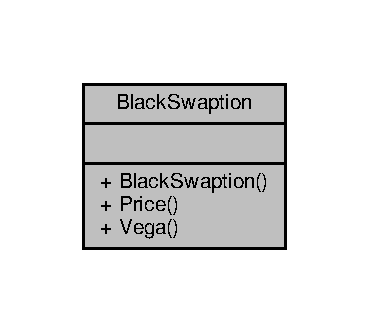
\includegraphics[width=177pt]{classBlackSwaption__coll__graph}
\end{center}
\end{figure}
\subsection*{Public Member Functions}
\begin{DoxyCompactItemize}
\item 
\hyperlink{classBlackSwaption_a5680b8b03c67b029749f43a907170258}{Black\+Swaption} (double annuity\+\_\+, double swap\+\_\+rate\+\_\+, double strike\+\_\+, double expiry\+\_\+)
\item 
double \hyperlink{classBlackSwaption_a87dea283a7e04dc04179e4b7014dd2e5}{Price} (double vol) const
\item 
double \hyperlink{classBlackSwaption_aa9f453250bb164887463ae41be3fca17}{Vega} (double vol) const
\end{DoxyCompactItemize}


\subsection{Constructor \& Destructor Documentation}
\hypertarget{classBlackSwaption_a5680b8b03c67b029749f43a907170258}{}\label{classBlackSwaption_a5680b8b03c67b029749f43a907170258} 
\index{Black\+Swaption@{Black\+Swaption}!Black\+Swaption@{Black\+Swaption}}
\index{Black\+Swaption@{Black\+Swaption}!Black\+Swaption@{Black\+Swaption}}
\subsubsection{\texorpdfstring{Black\+Swaption()}{BlackSwaption()}}
{\footnotesize\ttfamily Black\+Swaption\+::\+Black\+Swaption (\begin{DoxyParamCaption}\item[{double}]{annuity\+\_\+,  }\item[{double}]{swap\+\_\+rate\+\_\+,  }\item[{double}]{strike\+\_\+,  }\item[{double}]{expiry\+\_\+ }\end{DoxyParamCaption})}



\subsection{Member Function Documentation}
\hypertarget{classBlackSwaption_a87dea283a7e04dc04179e4b7014dd2e5}{}\label{classBlackSwaption_a87dea283a7e04dc04179e4b7014dd2e5} 
\index{Black\+Swaption@{Black\+Swaption}!Price@{Price}}
\index{Price@{Price}!Black\+Swaption@{Black\+Swaption}}
\subsubsection{\texorpdfstring{Price()}{Price()}}
{\footnotesize\ttfamily double Black\+Swaption\+::\+Price (\begin{DoxyParamCaption}\item[{double}]{vol }\end{DoxyParamCaption}) const}

\hypertarget{classBlackSwaption_aa9f453250bb164887463ae41be3fca17}{}\label{classBlackSwaption_aa9f453250bb164887463ae41be3fca17} 
\index{Black\+Swaption@{Black\+Swaption}!Vega@{Vega}}
\index{Vega@{Vega}!Black\+Swaption@{Black\+Swaption}}
\subsubsection{\texorpdfstring{Vega()}{Vega()}}
{\footnotesize\ttfamily double Black\+Swaption\+::\+Vega (\begin{DoxyParamCaption}\item[{double}]{vol }\end{DoxyParamCaption}) const}



The documentation for this class was generated from the following file\+:\begin{DoxyCompactItemize}
\item 
\hyperlink{BlackSwaption_8h}{Black\+Swaption.\+h}\end{DoxyCompactItemize}

\hypertarget{classBSCall}{}\section{B\+S\+Call Class Reference}
\label{classBSCall}\index{B\+S\+Call@{B\+S\+Call}}


{\ttfamily \#include $<$B\+S\+Call\+Class.\+h$>$}



Collaboration diagram for B\+S\+Call\+:
\nopagebreak
\begin{figure}[H]
\begin{center}
\leavevmode
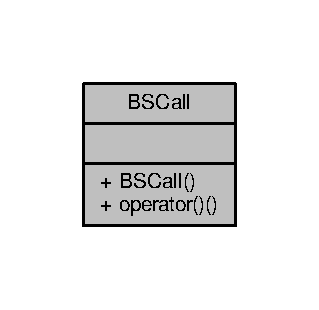
\includegraphics[width=153pt]{classBSCall__coll__graph}
\end{center}
\end{figure}
\subsection*{Public Member Functions}
\begin{DoxyCompactItemize}
\item 
\hyperlink{classBSCall_abe2b43379fddbc8fe0ef9a4173b87608}{B\+S\+Call} (double r\+\_\+, double d\+\_\+, double T, double Spot\+\_\+, double Strike\+\_\+)
\item 
double \hyperlink{classBSCall_a98d2d6613888711c773492520b881e2a}{operator()} (double Vol) const
\end{DoxyCompactItemize}


\subsection{Constructor \& Destructor Documentation}
\hypertarget{classBSCall_abe2b43379fddbc8fe0ef9a4173b87608}{}\label{classBSCall_abe2b43379fddbc8fe0ef9a4173b87608} 
\index{B\+S\+Call@{B\+S\+Call}!B\+S\+Call@{B\+S\+Call}}
\index{B\+S\+Call@{B\+S\+Call}!B\+S\+Call@{B\+S\+Call}}
\subsubsection{\texorpdfstring{B\+S\+Call()}{BSCall()}}
{\footnotesize\ttfamily B\+S\+Call\+::\+B\+S\+Call (\begin{DoxyParamCaption}\item[{double}]{r\+\_\+,  }\item[{double}]{d\+\_\+,  }\item[{double}]{T,  }\item[{double}]{Spot\+\_\+,  }\item[{double}]{Strike\+\_\+ }\end{DoxyParamCaption})}



\subsection{Member Function Documentation}
\hypertarget{classBSCall_a98d2d6613888711c773492520b881e2a}{}\label{classBSCall_a98d2d6613888711c773492520b881e2a} 
\index{B\+S\+Call@{B\+S\+Call}!operator()@{operator()}}
\index{operator()@{operator()}!B\+S\+Call@{B\+S\+Call}}
\subsubsection{\texorpdfstring{operator()()}{operator()()}}
{\footnotesize\ttfamily double B\+S\+Call\+::operator() (\begin{DoxyParamCaption}\item[{double}]{Vol }\end{DoxyParamCaption}) const}



The documentation for this class was generated from the following file\+:\begin{DoxyCompactItemize}
\item 
\hyperlink{BSCallClass_8h}{B\+S\+Call\+Class.\+h}\end{DoxyCompactItemize}

\hypertarget{classBSCallTwo}{}\section{B\+S\+Call\+Two Class Reference}
\label{classBSCallTwo}\index{B\+S\+Call\+Two@{B\+S\+Call\+Two}}


{\ttfamily \#include $<$B\+S\+Call\+Two.\+h$>$}



Collaboration diagram for B\+S\+Call\+Two\+:
\nopagebreak
\begin{figure}[H]
\begin{center}
\leavevmode
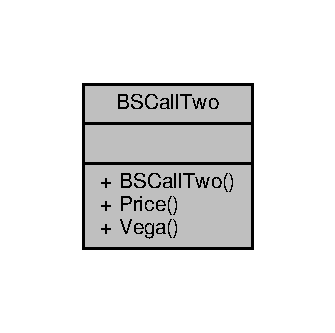
\includegraphics[width=161pt]{classBSCallTwo__coll__graph}
\end{center}
\end{figure}
\subsection*{Public Member Functions}
\begin{DoxyCompactItemize}
\item 
\hyperlink{classBSCallTwo_aec615c8420082c0bd886521faa9643d8}{B\+S\+Call\+Two} (double r\+\_\+, double d\+\_\+, double T, double Spot\+\_\+, double Strike\+\_\+)
\item 
double \hyperlink{classBSCallTwo_a665a1b79a859410d1b588c0811f4143a}{Price} (double Vol) const
\item 
double \hyperlink{classBSCallTwo_ab98dc7e0e5218cfc47aac07c700539fa}{Vega} (double Vol) const
\end{DoxyCompactItemize}


\subsection{Constructor \& Destructor Documentation}
\hypertarget{classBSCallTwo_aec615c8420082c0bd886521faa9643d8}{}\label{classBSCallTwo_aec615c8420082c0bd886521faa9643d8} 
\index{B\+S\+Call\+Two@{B\+S\+Call\+Two}!B\+S\+Call\+Two@{B\+S\+Call\+Two}}
\index{B\+S\+Call\+Two@{B\+S\+Call\+Two}!B\+S\+Call\+Two@{B\+S\+Call\+Two}}
\subsubsection{\texorpdfstring{B\+S\+Call\+Two()}{BSCallTwo()}}
{\footnotesize\ttfamily B\+S\+Call\+Two\+::\+B\+S\+Call\+Two (\begin{DoxyParamCaption}\item[{double}]{r\+\_\+,  }\item[{double}]{d\+\_\+,  }\item[{double}]{T,  }\item[{double}]{Spot\+\_\+,  }\item[{double}]{Strike\+\_\+ }\end{DoxyParamCaption})}



\subsection{Member Function Documentation}
\hypertarget{classBSCallTwo_a665a1b79a859410d1b588c0811f4143a}{}\label{classBSCallTwo_a665a1b79a859410d1b588c0811f4143a} 
\index{B\+S\+Call\+Two@{B\+S\+Call\+Two}!Price@{Price}}
\index{Price@{Price}!B\+S\+Call\+Two@{B\+S\+Call\+Two}}
\subsubsection{\texorpdfstring{Price()}{Price()}}
{\footnotesize\ttfamily double B\+S\+Call\+Two\+::\+Price (\begin{DoxyParamCaption}\item[{double}]{Vol }\end{DoxyParamCaption}) const}

\hypertarget{classBSCallTwo_ab98dc7e0e5218cfc47aac07c700539fa}{}\label{classBSCallTwo_ab98dc7e0e5218cfc47aac07c700539fa} 
\index{B\+S\+Call\+Two@{B\+S\+Call\+Two}!Vega@{Vega}}
\index{Vega@{Vega}!B\+S\+Call\+Two@{B\+S\+Call\+Two}}
\subsubsection{\texorpdfstring{Vega()}{Vega()}}
{\footnotesize\ttfamily double B\+S\+Call\+Two\+::\+Vega (\begin{DoxyParamCaption}\item[{double}]{Vol }\end{DoxyParamCaption}) const}



The documentation for this class was generated from the following file\+:\begin{DoxyCompactItemize}
\item 
\hyperlink{BSCallTwo_8h}{B\+S\+Call\+Two.\+h}\end{DoxyCompactItemize}

\hypertarget{classMyOption_1_1CallOption}{}\section{My\+Option\+:\+:Call\+Option Class Reference}
\label{classMyOption_1_1CallOption}\index{My\+Option\+::\+Call\+Option@{My\+Option\+::\+Call\+Option}}


{\ttfamily \#include $<$options.\+h$>$}



Inheritance diagram for My\+Option\+:\+:Call\+Option\+:
\nopagebreak
\begin{figure}[H]
\begin{center}
\leavevmode
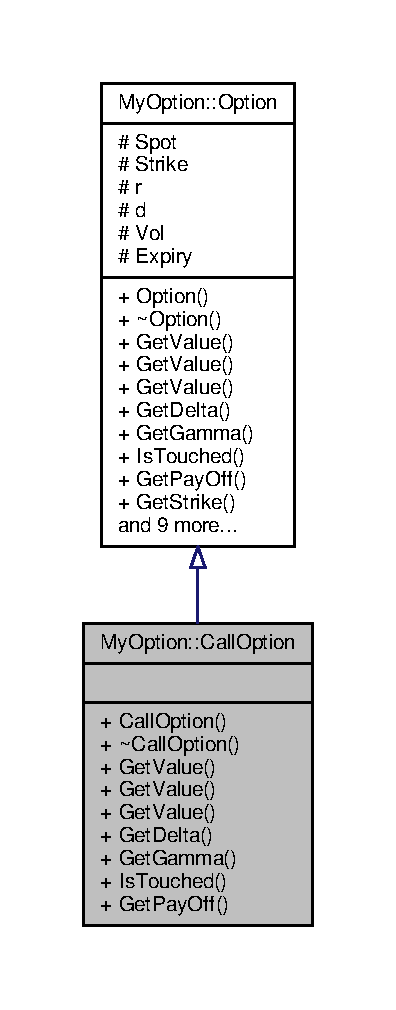
\includegraphics[width=190pt]{classMyOption_1_1CallOption__inherit__graph}
\end{center}
\end{figure}


Collaboration diagram for My\+Option\+:\+:Call\+Option\+:
\nopagebreak
\begin{figure}[H]
\begin{center}
\leavevmode
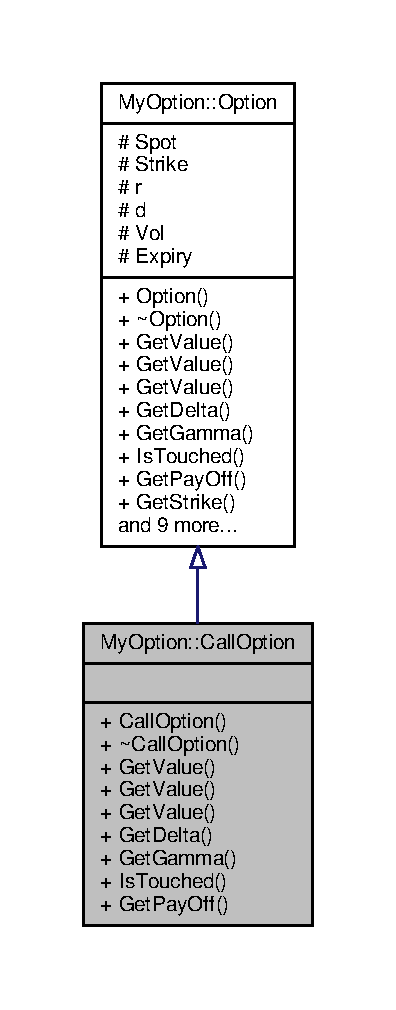
\includegraphics[width=190pt]{classMyOption_1_1CallOption__coll__graph}
\end{center}
\end{figure}
\subsection*{Public Member Functions}
\begin{DoxyCompactItemize}
\item 
\hyperlink{classMyOption_1_1CallOption_acca66308420dd80fa525698a77fb53c4}{Call\+Option} (double \hyperlink{classMyOption_1_1Option_a6c6f01d75cde7e92d16a6d8d6f331a1d}{Spot}, double \hyperlink{classMyOption_1_1Option_a3033c483588ce26b175280c7f9dee8d1}{Strike}, double \hyperlink{classMyOption_1_1Option_aa8cb250427dece65ea49255d4102cc8d}{r}, double \hyperlink{classMyOption_1_1Option_a500979f4b32262594d895c4a83b58d1d}{d}, double \hyperlink{classMyOption_1_1Option_a5d6002c14b335c782873bf1437113513}{Vol}, double \hyperlink{classMyOption_1_1Option_ac1adacb417fede41d151b9cda05bcb3d}{Expiry})
\item 
virtual \hyperlink{classMyOption_1_1CallOption_a1b6b001899368335db393aa8050c9a5c}{$\sim$\+Call\+Option} ()
\item 
virtual double \hyperlink{classMyOption_1_1CallOption_a89cec28009a9c940504b13357842bb49}{Get\+Value} (double \hyperlink{classMyOption_1_1Option_a6c6f01d75cde7e92d16a6d8d6f331a1d}{Spot})
\item 
virtual double \hyperlink{classMyOption_1_1CallOption_a19f1aab1a885c9520c033fc27706777e}{Get\+Value} (double \hyperlink{classMyOption_1_1Option_a6c6f01d75cde7e92d16a6d8d6f331a1d}{Spot}, double \hyperlink{classMyOption_1_1Option_a5d6002c14b335c782873bf1437113513}{Vol}, double \hyperlink{classMyOption_1_1Option_ac1adacb417fede41d151b9cda05bcb3d}{Expiry})
\item 
virtual double \hyperlink{classMyOption_1_1CallOption_a2a3ca51422260a20ac9d151f38980df7}{Get\+Value} (double \hyperlink{classMyOption_1_1Option_a6c6f01d75cde7e92d16a6d8d6f331a1d}{Spot}, double \hyperlink{classMyOption_1_1Option_aa8cb250427dece65ea49255d4102cc8d}{r}, double \hyperlink{classMyOption_1_1Option_a5d6002c14b335c782873bf1437113513}{Vol}, double \hyperlink{classMyOption_1_1Option_ac1adacb417fede41d151b9cda05bcb3d}{Expiry})
\item 
virtual double \hyperlink{classMyOption_1_1CallOption_a46b6e6aa7b12967b825f50ec66911e51}{Get\+Delta} (double \hyperlink{classMyOption_1_1Option_a6c6f01d75cde7e92d16a6d8d6f331a1d}{Spot}, double \hyperlink{classMyOption_1_1Option_a5d6002c14b335c782873bf1437113513}{Vol}, double \hyperlink{classMyOption_1_1Option_ac1adacb417fede41d151b9cda05bcb3d}{Expiry})
\item 
virtual double \hyperlink{classMyOption_1_1CallOption_a135259127b922e4ce4db8243c3c52a54}{Get\+Gamma} (double \hyperlink{classMyOption_1_1Option_a6c6f01d75cde7e92d16a6d8d6f331a1d}{Spot}, double \hyperlink{classMyOption_1_1Option_a5d6002c14b335c782873bf1437113513}{Vol}, double \hyperlink{classMyOption_1_1Option_ac1adacb417fede41d151b9cda05bcb3d}{Expiry})
\item 
virtual long \hyperlink{classMyOption_1_1CallOption_a397e70701e8a882e0205193513d27b97}{Is\+Touched} (double \hyperlink{classMyOption_1_1Option_a6c6f01d75cde7e92d16a6d8d6f331a1d}{Spot}) const
\item 
virtual double \hyperlink{classMyOption_1_1CallOption_ad1ee991cfd969e450d7d227dee61be05}{Get\+Pay\+Off} (double \hyperlink{classMyOption_1_1Option_a6c6f01d75cde7e92d16a6d8d6f331a1d}{Spot}) const
\end{DoxyCompactItemize}
\subsection*{Additional Inherited Members}


\subsection{Constructor \& Destructor Documentation}
\hypertarget{classMyOption_1_1CallOption_acca66308420dd80fa525698a77fb53c4}{}\label{classMyOption_1_1CallOption_acca66308420dd80fa525698a77fb53c4} 
\index{My\+Option\+::\+Call\+Option@{My\+Option\+::\+Call\+Option}!Call\+Option@{Call\+Option}}
\index{Call\+Option@{Call\+Option}!My\+Option\+::\+Call\+Option@{My\+Option\+::\+Call\+Option}}
\subsubsection{\texorpdfstring{Call\+Option()}{CallOption()}}
{\footnotesize\ttfamily My\+Option\+::\+Call\+Option\+::\+Call\+Option (\begin{DoxyParamCaption}\item[{double}]{Spot,  }\item[{double}]{Strike,  }\item[{double}]{r,  }\item[{double}]{d,  }\item[{double}]{Vol,  }\item[{double}]{Expiry }\end{DoxyParamCaption})}

\hypertarget{classMyOption_1_1CallOption_a1b6b001899368335db393aa8050c9a5c}{}\label{classMyOption_1_1CallOption_a1b6b001899368335db393aa8050c9a5c} 
\index{My\+Option\+::\+Call\+Option@{My\+Option\+::\+Call\+Option}!````~Call\+Option@{$\sim$\+Call\+Option}}
\index{````~Call\+Option@{$\sim$\+Call\+Option}!My\+Option\+::\+Call\+Option@{My\+Option\+::\+Call\+Option}}
\subsubsection{\texorpdfstring{$\sim$\+Call\+Option()}{~CallOption()}}
{\footnotesize\ttfamily virtual My\+Option\+::\+Call\+Option\+::$\sim$\+Call\+Option (\begin{DoxyParamCaption}{ }\end{DoxyParamCaption})\hspace{0.3cm}{\ttfamily [inline]}, {\ttfamily [virtual]}}



\subsection{Member Function Documentation}
\hypertarget{classMyOption_1_1CallOption_a46b6e6aa7b12967b825f50ec66911e51}{}\label{classMyOption_1_1CallOption_a46b6e6aa7b12967b825f50ec66911e51} 
\index{My\+Option\+::\+Call\+Option@{My\+Option\+::\+Call\+Option}!Get\+Delta@{Get\+Delta}}
\index{Get\+Delta@{Get\+Delta}!My\+Option\+::\+Call\+Option@{My\+Option\+::\+Call\+Option}}
\subsubsection{\texorpdfstring{Get\+Delta()}{GetDelta()}}
{\footnotesize\ttfamily virtual double My\+Option\+::\+Call\+Option\+::\+Get\+Delta (\begin{DoxyParamCaption}\item[{double}]{Spot,  }\item[{double}]{Vol,  }\item[{double}]{Expiry }\end{DoxyParamCaption})\hspace{0.3cm}{\ttfamily [virtual]}}



Implements \hyperlink{classMyOption_1_1Option_a4947bde99bb5e46b79aa0f36fd353d9b}{My\+Option\+::\+Option}.

\hypertarget{classMyOption_1_1CallOption_a135259127b922e4ce4db8243c3c52a54}{}\label{classMyOption_1_1CallOption_a135259127b922e4ce4db8243c3c52a54} 
\index{My\+Option\+::\+Call\+Option@{My\+Option\+::\+Call\+Option}!Get\+Gamma@{Get\+Gamma}}
\index{Get\+Gamma@{Get\+Gamma}!My\+Option\+::\+Call\+Option@{My\+Option\+::\+Call\+Option}}
\subsubsection{\texorpdfstring{Get\+Gamma()}{GetGamma()}}
{\footnotesize\ttfamily virtual double My\+Option\+::\+Call\+Option\+::\+Get\+Gamma (\begin{DoxyParamCaption}\item[{double}]{Spot,  }\item[{double}]{Vol,  }\item[{double}]{Expiry }\end{DoxyParamCaption})\hspace{0.3cm}{\ttfamily [virtual]}}



Implements \hyperlink{classMyOption_1_1Option_a4416faa432b5004e449394056c7f1363}{My\+Option\+::\+Option}.

\hypertarget{classMyOption_1_1CallOption_ad1ee991cfd969e450d7d227dee61be05}{}\label{classMyOption_1_1CallOption_ad1ee991cfd969e450d7d227dee61be05} 
\index{My\+Option\+::\+Call\+Option@{My\+Option\+::\+Call\+Option}!Get\+Pay\+Off@{Get\+Pay\+Off}}
\index{Get\+Pay\+Off@{Get\+Pay\+Off}!My\+Option\+::\+Call\+Option@{My\+Option\+::\+Call\+Option}}
\subsubsection{\texorpdfstring{Get\+Pay\+Off()}{GetPayOff()}}
{\footnotesize\ttfamily virtual double My\+Option\+::\+Call\+Option\+::\+Get\+Pay\+Off (\begin{DoxyParamCaption}\item[{double}]{Spot }\end{DoxyParamCaption}) const\hspace{0.3cm}{\ttfamily [virtual]}}



Implements \hyperlink{classMyOption_1_1Option_a4b6b84dc485153ffadfb32afa9bb52f3}{My\+Option\+::\+Option}.

\hypertarget{classMyOption_1_1CallOption_a89cec28009a9c940504b13357842bb49}{}\label{classMyOption_1_1CallOption_a89cec28009a9c940504b13357842bb49} 
\index{My\+Option\+::\+Call\+Option@{My\+Option\+::\+Call\+Option}!Get\+Value@{Get\+Value}}
\index{Get\+Value@{Get\+Value}!My\+Option\+::\+Call\+Option@{My\+Option\+::\+Call\+Option}}
\subsubsection{\texorpdfstring{Get\+Value()}{GetValue()}\hspace{0.1cm}{\footnotesize\ttfamily [1/3]}}
{\footnotesize\ttfamily virtual double My\+Option\+::\+Call\+Option\+::\+Get\+Value (\begin{DoxyParamCaption}\item[{double}]{Spot }\end{DoxyParamCaption})\hspace{0.3cm}{\ttfamily [virtual]}}



Implements \hyperlink{classMyOption_1_1Option_aff32b402a5e44fca9e5a22a142fbbdd6}{My\+Option\+::\+Option}.

\hypertarget{classMyOption_1_1CallOption_a19f1aab1a885c9520c033fc27706777e}{}\label{classMyOption_1_1CallOption_a19f1aab1a885c9520c033fc27706777e} 
\index{My\+Option\+::\+Call\+Option@{My\+Option\+::\+Call\+Option}!Get\+Value@{Get\+Value}}
\index{Get\+Value@{Get\+Value}!My\+Option\+::\+Call\+Option@{My\+Option\+::\+Call\+Option}}
\subsubsection{\texorpdfstring{Get\+Value()}{GetValue()}\hspace{0.1cm}{\footnotesize\ttfamily [2/3]}}
{\footnotesize\ttfamily virtual double My\+Option\+::\+Call\+Option\+::\+Get\+Value (\begin{DoxyParamCaption}\item[{double}]{Spot,  }\item[{double}]{Vol,  }\item[{double}]{Expiry }\end{DoxyParamCaption})\hspace{0.3cm}{\ttfamily [virtual]}}



Implements \hyperlink{classMyOption_1_1Option_a78fa248dcb939e0ebaefbb944d5d9cf8}{My\+Option\+::\+Option}.

\hypertarget{classMyOption_1_1CallOption_a2a3ca51422260a20ac9d151f38980df7}{}\label{classMyOption_1_1CallOption_a2a3ca51422260a20ac9d151f38980df7} 
\index{My\+Option\+::\+Call\+Option@{My\+Option\+::\+Call\+Option}!Get\+Value@{Get\+Value}}
\index{Get\+Value@{Get\+Value}!My\+Option\+::\+Call\+Option@{My\+Option\+::\+Call\+Option}}
\subsubsection{\texorpdfstring{Get\+Value()}{GetValue()}\hspace{0.1cm}{\footnotesize\ttfamily [3/3]}}
{\footnotesize\ttfamily virtual double My\+Option\+::\+Call\+Option\+::\+Get\+Value (\begin{DoxyParamCaption}\item[{double}]{Spot,  }\item[{double}]{r,  }\item[{double}]{Vol,  }\item[{double}]{Expiry }\end{DoxyParamCaption})\hspace{0.3cm}{\ttfamily [virtual]}}



Implements \hyperlink{classMyOption_1_1Option_a62422d3dc60eabe65cfa94d2a452f5f8}{My\+Option\+::\+Option}.

\hypertarget{classMyOption_1_1CallOption_a397e70701e8a882e0205193513d27b97}{}\label{classMyOption_1_1CallOption_a397e70701e8a882e0205193513d27b97} 
\index{My\+Option\+::\+Call\+Option@{My\+Option\+::\+Call\+Option}!Is\+Touched@{Is\+Touched}}
\index{Is\+Touched@{Is\+Touched}!My\+Option\+::\+Call\+Option@{My\+Option\+::\+Call\+Option}}
\subsubsection{\texorpdfstring{Is\+Touched()}{IsTouched()}}
{\footnotesize\ttfamily virtual long My\+Option\+::\+Call\+Option\+::\+Is\+Touched (\begin{DoxyParamCaption}\item[{double}]{Spot }\end{DoxyParamCaption}) const\hspace{0.3cm}{\ttfamily [virtual]}}



Implements \hyperlink{classMyOption_1_1Option_ade57d2fcb9f22f3c2a57d75f55444c33}{My\+Option\+::\+Option}.



The documentation for this class was generated from the following file\+:\begin{DoxyCompactItemize}
\item 
\hyperlink{options_8h}{options.\+h}\end{DoxyCompactItemize}

\hypertarget{classMyOption_1_1CallSpreadOption}{}\section{My\+Option\+:\+:Call\+Spread\+Option Class Reference}
\label{classMyOption_1_1CallSpreadOption}\index{My\+Option\+::\+Call\+Spread\+Option@{My\+Option\+::\+Call\+Spread\+Option}}


{\ttfamily \#include $<$options.\+h$>$}



Inheritance diagram for My\+Option\+:\+:Call\+Spread\+Option\+:
\nopagebreak
\begin{figure}[H]
\begin{center}
\leavevmode
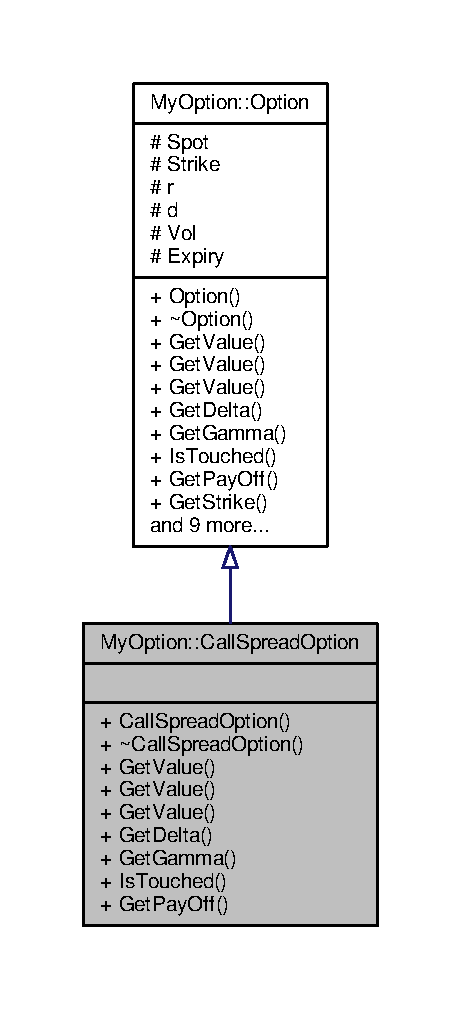
\includegraphics[width=221pt]{classMyOption_1_1CallSpreadOption__inherit__graph}
\end{center}
\end{figure}


Collaboration diagram for My\+Option\+:\+:Call\+Spread\+Option\+:
\nopagebreak
\begin{figure}[H]
\begin{center}
\leavevmode
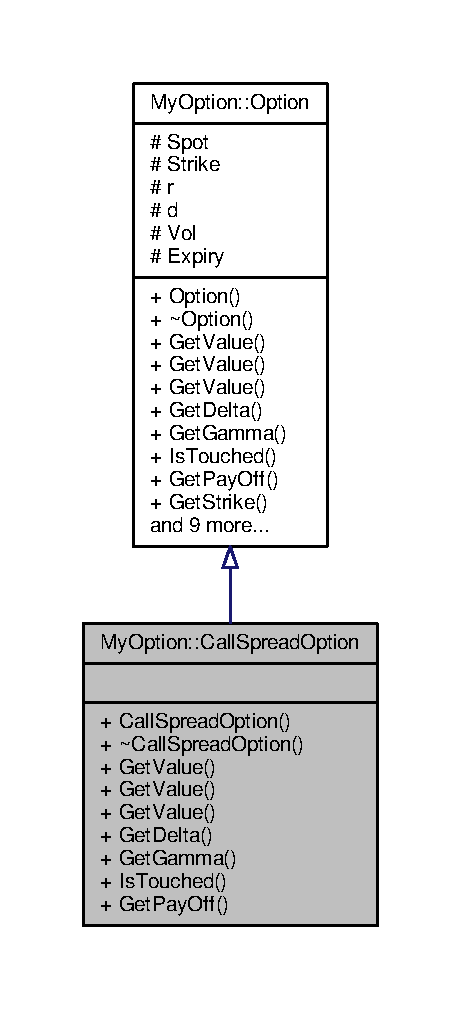
\includegraphics[width=221pt]{classMyOption_1_1CallSpreadOption__coll__graph}
\end{center}
\end{figure}
\subsection*{Public Member Functions}
\begin{DoxyCompactItemize}
\item 
\hyperlink{classMyOption_1_1CallSpreadOption_a5d9a2c5d587451e30c49aed0f48f4dc4}{Call\+Spread\+Option} (double \hyperlink{classMyOption_1_1Option_a6c6f01d75cde7e92d16a6d8d6f331a1d}{Spot}, double \hyperlink{classMyOption_1_1Option_a3033c483588ce26b175280c7f9dee8d1}{Strike}, double \hyperlink{classMyOption_1_1Option_aa8cb250427dece65ea49255d4102cc8d}{r}, double \hyperlink{classMyOption_1_1Option_a500979f4b32262594d895c4a83b58d1d}{d}, double \hyperlink{classMyOption_1_1Option_a5d6002c14b335c782873bf1437113513}{Vol}, double \hyperlink{classMyOption_1_1Option_ac1adacb417fede41d151b9cda05bcb3d}{Expiry}, double epsilon)
\item 
virtual \hyperlink{classMyOption_1_1CallSpreadOption_a20c0f91c648645718aa27007399101e7}{$\sim$\+Call\+Spread\+Option} ()
\item 
virtual double \hyperlink{classMyOption_1_1CallSpreadOption_a8f9317c21aad28bc1cd78a403b5e4cd3}{Get\+Value} (double \hyperlink{classMyOption_1_1Option_a6c6f01d75cde7e92d16a6d8d6f331a1d}{Spot})
\item 
virtual double \hyperlink{classMyOption_1_1CallSpreadOption_a99b187caf21ba9b6f505923d9e785c12}{Get\+Value} (double \hyperlink{classMyOption_1_1Option_a6c6f01d75cde7e92d16a6d8d6f331a1d}{Spot}, double \hyperlink{classMyOption_1_1Option_a5d6002c14b335c782873bf1437113513}{Vol}, double \hyperlink{classMyOption_1_1Option_ac1adacb417fede41d151b9cda05bcb3d}{Expiry})
\item 
virtual double \hyperlink{classMyOption_1_1CallSpreadOption_a5e88bf671572da6441db916620c5c202}{Get\+Value} (double \hyperlink{classMyOption_1_1Option_a6c6f01d75cde7e92d16a6d8d6f331a1d}{Spot}, double \hyperlink{classMyOption_1_1Option_aa8cb250427dece65ea49255d4102cc8d}{r}, double \hyperlink{classMyOption_1_1Option_a5d6002c14b335c782873bf1437113513}{Vol}, double \hyperlink{classMyOption_1_1Option_ac1adacb417fede41d151b9cda05bcb3d}{Expiry})
\item 
virtual double \hyperlink{classMyOption_1_1CallSpreadOption_a4655116155bf4551129eda47625acef0}{Get\+Delta} (double \hyperlink{classMyOption_1_1Option_a6c6f01d75cde7e92d16a6d8d6f331a1d}{Spot}, double \hyperlink{classMyOption_1_1Option_a5d6002c14b335c782873bf1437113513}{Vol}, double \hyperlink{classMyOption_1_1Option_ac1adacb417fede41d151b9cda05bcb3d}{Expiry})
\item 
virtual double \hyperlink{classMyOption_1_1CallSpreadOption_ac8dd9fdb03603013350d611e6931a314}{Get\+Gamma} (double \hyperlink{classMyOption_1_1Option_a6c6f01d75cde7e92d16a6d8d6f331a1d}{Spot}, double \hyperlink{classMyOption_1_1Option_a5d6002c14b335c782873bf1437113513}{Vol}, double \hyperlink{classMyOption_1_1Option_ac1adacb417fede41d151b9cda05bcb3d}{Expiry})
\item 
virtual long \hyperlink{classMyOption_1_1CallSpreadOption_a83f8cda1ab9e49df49f8d08d0bab23c7}{Is\+Touched} (double \hyperlink{classMyOption_1_1Option_a6c6f01d75cde7e92d16a6d8d6f331a1d}{Spot}) const
\item 
virtual double \hyperlink{classMyOption_1_1CallSpreadOption_a2e45ec109e4fd26acc6506caa1952c0c}{Get\+Pay\+Off} (double \hyperlink{classMyOption_1_1Option_a6c6f01d75cde7e92d16a6d8d6f331a1d}{Spot}) const
\end{DoxyCompactItemize}
\subsection*{Additional Inherited Members}


\subsection{Constructor \& Destructor Documentation}
\hypertarget{classMyOption_1_1CallSpreadOption_a5d9a2c5d587451e30c49aed0f48f4dc4}{}\label{classMyOption_1_1CallSpreadOption_a5d9a2c5d587451e30c49aed0f48f4dc4} 
\index{My\+Option\+::\+Call\+Spread\+Option@{My\+Option\+::\+Call\+Spread\+Option}!Call\+Spread\+Option@{Call\+Spread\+Option}}
\index{Call\+Spread\+Option@{Call\+Spread\+Option}!My\+Option\+::\+Call\+Spread\+Option@{My\+Option\+::\+Call\+Spread\+Option}}
\subsubsection{\texorpdfstring{Call\+Spread\+Option()}{CallSpreadOption()}}
{\footnotesize\ttfamily My\+Option\+::\+Call\+Spread\+Option\+::\+Call\+Spread\+Option (\begin{DoxyParamCaption}\item[{double}]{Spot,  }\item[{double}]{Strike,  }\item[{double}]{r,  }\item[{double}]{d,  }\item[{double}]{Vol,  }\item[{double}]{Expiry,  }\item[{double}]{epsilon }\end{DoxyParamCaption})}

\hypertarget{classMyOption_1_1CallSpreadOption_a20c0f91c648645718aa27007399101e7}{}\label{classMyOption_1_1CallSpreadOption_a20c0f91c648645718aa27007399101e7} 
\index{My\+Option\+::\+Call\+Spread\+Option@{My\+Option\+::\+Call\+Spread\+Option}!````~Call\+Spread\+Option@{$\sim$\+Call\+Spread\+Option}}
\index{````~Call\+Spread\+Option@{$\sim$\+Call\+Spread\+Option}!My\+Option\+::\+Call\+Spread\+Option@{My\+Option\+::\+Call\+Spread\+Option}}
\subsubsection{\texorpdfstring{$\sim$\+Call\+Spread\+Option()}{~CallSpreadOption()}}
{\footnotesize\ttfamily virtual My\+Option\+::\+Call\+Spread\+Option\+::$\sim$\+Call\+Spread\+Option (\begin{DoxyParamCaption}{ }\end{DoxyParamCaption})\hspace{0.3cm}{\ttfamily [inline]}, {\ttfamily [virtual]}}



\subsection{Member Function Documentation}
\hypertarget{classMyOption_1_1CallSpreadOption_a4655116155bf4551129eda47625acef0}{}\label{classMyOption_1_1CallSpreadOption_a4655116155bf4551129eda47625acef0} 
\index{My\+Option\+::\+Call\+Spread\+Option@{My\+Option\+::\+Call\+Spread\+Option}!Get\+Delta@{Get\+Delta}}
\index{Get\+Delta@{Get\+Delta}!My\+Option\+::\+Call\+Spread\+Option@{My\+Option\+::\+Call\+Spread\+Option}}
\subsubsection{\texorpdfstring{Get\+Delta()}{GetDelta()}}
{\footnotesize\ttfamily virtual double My\+Option\+::\+Call\+Spread\+Option\+::\+Get\+Delta (\begin{DoxyParamCaption}\item[{double}]{Spot,  }\item[{double}]{Vol,  }\item[{double}]{Expiry }\end{DoxyParamCaption})\hspace{0.3cm}{\ttfamily [virtual]}}



Implements \hyperlink{classMyOption_1_1Option_a4947bde99bb5e46b79aa0f36fd353d9b}{My\+Option\+::\+Option}.

\hypertarget{classMyOption_1_1CallSpreadOption_ac8dd9fdb03603013350d611e6931a314}{}\label{classMyOption_1_1CallSpreadOption_ac8dd9fdb03603013350d611e6931a314} 
\index{My\+Option\+::\+Call\+Spread\+Option@{My\+Option\+::\+Call\+Spread\+Option}!Get\+Gamma@{Get\+Gamma}}
\index{Get\+Gamma@{Get\+Gamma}!My\+Option\+::\+Call\+Spread\+Option@{My\+Option\+::\+Call\+Spread\+Option}}
\subsubsection{\texorpdfstring{Get\+Gamma()}{GetGamma()}}
{\footnotesize\ttfamily virtual double My\+Option\+::\+Call\+Spread\+Option\+::\+Get\+Gamma (\begin{DoxyParamCaption}\item[{double}]{Spot,  }\item[{double}]{Vol,  }\item[{double}]{Expiry }\end{DoxyParamCaption})\hspace{0.3cm}{\ttfamily [virtual]}}



Implements \hyperlink{classMyOption_1_1Option_a4416faa432b5004e449394056c7f1363}{My\+Option\+::\+Option}.

\hypertarget{classMyOption_1_1CallSpreadOption_a2e45ec109e4fd26acc6506caa1952c0c}{}\label{classMyOption_1_1CallSpreadOption_a2e45ec109e4fd26acc6506caa1952c0c} 
\index{My\+Option\+::\+Call\+Spread\+Option@{My\+Option\+::\+Call\+Spread\+Option}!Get\+Pay\+Off@{Get\+Pay\+Off}}
\index{Get\+Pay\+Off@{Get\+Pay\+Off}!My\+Option\+::\+Call\+Spread\+Option@{My\+Option\+::\+Call\+Spread\+Option}}
\subsubsection{\texorpdfstring{Get\+Pay\+Off()}{GetPayOff()}}
{\footnotesize\ttfamily virtual double My\+Option\+::\+Call\+Spread\+Option\+::\+Get\+Pay\+Off (\begin{DoxyParamCaption}\item[{double}]{Spot }\end{DoxyParamCaption}) const\hspace{0.3cm}{\ttfamily [virtual]}}



Implements \hyperlink{classMyOption_1_1Option_a4b6b84dc485153ffadfb32afa9bb52f3}{My\+Option\+::\+Option}.

\hypertarget{classMyOption_1_1CallSpreadOption_a8f9317c21aad28bc1cd78a403b5e4cd3}{}\label{classMyOption_1_1CallSpreadOption_a8f9317c21aad28bc1cd78a403b5e4cd3} 
\index{My\+Option\+::\+Call\+Spread\+Option@{My\+Option\+::\+Call\+Spread\+Option}!Get\+Value@{Get\+Value}}
\index{Get\+Value@{Get\+Value}!My\+Option\+::\+Call\+Spread\+Option@{My\+Option\+::\+Call\+Spread\+Option}}
\subsubsection{\texorpdfstring{Get\+Value()}{GetValue()}\hspace{0.1cm}{\footnotesize\ttfamily [1/3]}}
{\footnotesize\ttfamily virtual double My\+Option\+::\+Call\+Spread\+Option\+::\+Get\+Value (\begin{DoxyParamCaption}\item[{double}]{Spot }\end{DoxyParamCaption})\hspace{0.3cm}{\ttfamily [virtual]}}



Implements \hyperlink{classMyOption_1_1Option_aff32b402a5e44fca9e5a22a142fbbdd6}{My\+Option\+::\+Option}.

\hypertarget{classMyOption_1_1CallSpreadOption_a99b187caf21ba9b6f505923d9e785c12}{}\label{classMyOption_1_1CallSpreadOption_a99b187caf21ba9b6f505923d9e785c12} 
\index{My\+Option\+::\+Call\+Spread\+Option@{My\+Option\+::\+Call\+Spread\+Option}!Get\+Value@{Get\+Value}}
\index{Get\+Value@{Get\+Value}!My\+Option\+::\+Call\+Spread\+Option@{My\+Option\+::\+Call\+Spread\+Option}}
\subsubsection{\texorpdfstring{Get\+Value()}{GetValue()}\hspace{0.1cm}{\footnotesize\ttfamily [2/3]}}
{\footnotesize\ttfamily virtual double My\+Option\+::\+Call\+Spread\+Option\+::\+Get\+Value (\begin{DoxyParamCaption}\item[{double}]{Spot,  }\item[{double}]{Vol,  }\item[{double}]{Expiry }\end{DoxyParamCaption})\hspace{0.3cm}{\ttfamily [virtual]}}



Implements \hyperlink{classMyOption_1_1Option_a78fa248dcb939e0ebaefbb944d5d9cf8}{My\+Option\+::\+Option}.

\hypertarget{classMyOption_1_1CallSpreadOption_a5e88bf671572da6441db916620c5c202}{}\label{classMyOption_1_1CallSpreadOption_a5e88bf671572da6441db916620c5c202} 
\index{My\+Option\+::\+Call\+Spread\+Option@{My\+Option\+::\+Call\+Spread\+Option}!Get\+Value@{Get\+Value}}
\index{Get\+Value@{Get\+Value}!My\+Option\+::\+Call\+Spread\+Option@{My\+Option\+::\+Call\+Spread\+Option}}
\subsubsection{\texorpdfstring{Get\+Value()}{GetValue()}\hspace{0.1cm}{\footnotesize\ttfamily [3/3]}}
{\footnotesize\ttfamily virtual double My\+Option\+::\+Call\+Spread\+Option\+::\+Get\+Value (\begin{DoxyParamCaption}\item[{double}]{Spot,  }\item[{double}]{r,  }\item[{double}]{Vol,  }\item[{double}]{Expiry }\end{DoxyParamCaption})\hspace{0.3cm}{\ttfamily [virtual]}}



Implements \hyperlink{classMyOption_1_1Option_a62422d3dc60eabe65cfa94d2a452f5f8}{My\+Option\+::\+Option}.

\hypertarget{classMyOption_1_1CallSpreadOption_a83f8cda1ab9e49df49f8d08d0bab23c7}{}\label{classMyOption_1_1CallSpreadOption_a83f8cda1ab9e49df49f8d08d0bab23c7} 
\index{My\+Option\+::\+Call\+Spread\+Option@{My\+Option\+::\+Call\+Spread\+Option}!Is\+Touched@{Is\+Touched}}
\index{Is\+Touched@{Is\+Touched}!My\+Option\+::\+Call\+Spread\+Option@{My\+Option\+::\+Call\+Spread\+Option}}
\subsubsection{\texorpdfstring{Is\+Touched()}{IsTouched()}}
{\footnotesize\ttfamily virtual long My\+Option\+::\+Call\+Spread\+Option\+::\+Is\+Touched (\begin{DoxyParamCaption}\item[{double}]{Spot }\end{DoxyParamCaption}) const\hspace{0.3cm}{\ttfamily [virtual]}}



Implements \hyperlink{classMyOption_1_1Option_ade57d2fcb9f22f3c2a57d75f55444c33}{My\+Option\+::\+Option}.



The documentation for this class was generated from the following file\+:\begin{DoxyCompactItemize}
\item 
\hyperlink{options_8h}{options.\+h}\end{DoxyCompactItemize}

\hypertarget{classCaplet}{}\section{Caplet Class Reference}
\label{classCaplet}\index{Caplet@{Caplet}}


{\ttfamily \#include $<$payoff\+\_\+interest\+\_\+derivatives.\+h$>$}



Inheritance diagram for Caplet\+:
\nopagebreak
\begin{figure}[H]
\begin{center}
\leavevmode
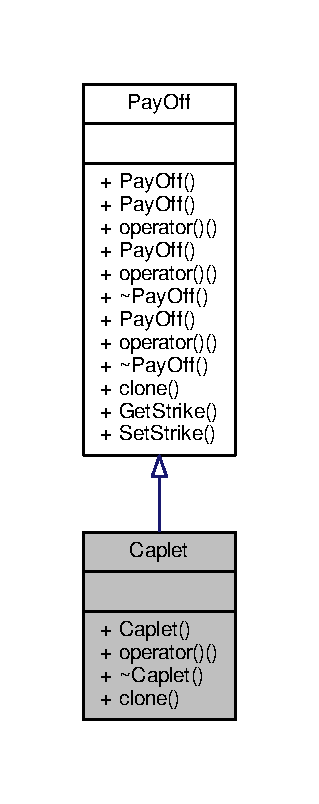
\includegraphics[width=153pt]{classCaplet__inherit__graph}
\end{center}
\end{figure}


Collaboration diagram for Caplet\+:
\nopagebreak
\begin{figure}[H]
\begin{center}
\leavevmode
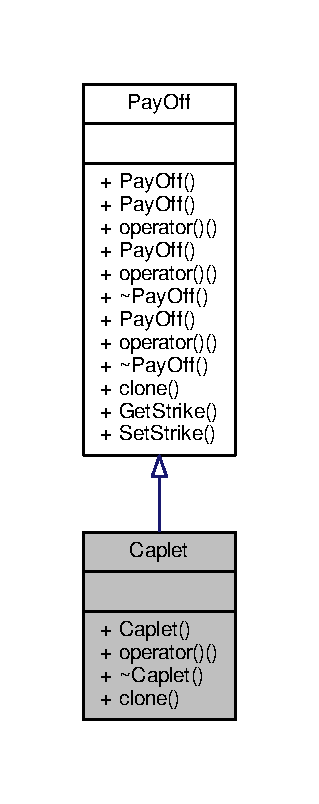
\includegraphics[width=153pt]{classCaplet__coll__graph}
\end{center}
\end{figure}
\subsection*{Public Member Functions}
\begin{DoxyCompactItemize}
\item 
\hyperlink{classCaplet_a350941f2d902ebcc9332bd2dc33e442a}{Caplet} (double Strike\+\_\+, double t1\+\_\+, double t2\+\_\+)
\item 
virtual double \hyperlink{classCaplet_a6b75d621f3c7631b50b7486306466daa}{operator()} (double Spot) const
\item 
virtual \hyperlink{classCaplet_ac0fad0b6aeef3bd1d2d88d280ebd5072}{$\sim$\+Caplet} ()
\item 
virtual \hyperlink{classPayOff}{Pay\+Off} $\ast$ \hyperlink{classCaplet_aeadd950733f02c066c474badceb277ef}{clone} () const
\end{DoxyCompactItemize}
\subsection*{Additional Inherited Members}


\subsection{Constructor \& Destructor Documentation}
\hypertarget{classCaplet_a350941f2d902ebcc9332bd2dc33e442a}{}\label{classCaplet_a350941f2d902ebcc9332bd2dc33e442a} 
\index{Caplet@{Caplet}!Caplet@{Caplet}}
\index{Caplet@{Caplet}!Caplet@{Caplet}}
\subsubsection{\texorpdfstring{Caplet()}{Caplet()}}
{\footnotesize\ttfamily Caplet\+::\+Caplet (\begin{DoxyParamCaption}\item[{double}]{Strike\+\_\+,  }\item[{double}]{t1\+\_\+,  }\item[{double}]{t2\+\_\+ }\end{DoxyParamCaption})}

\hypertarget{classCaplet_ac0fad0b6aeef3bd1d2d88d280ebd5072}{}\label{classCaplet_ac0fad0b6aeef3bd1d2d88d280ebd5072} 
\index{Caplet@{Caplet}!````~Caplet@{$\sim$\+Caplet}}
\index{````~Caplet@{$\sim$\+Caplet}!Caplet@{Caplet}}
\subsubsection{\texorpdfstring{$\sim$\+Caplet()}{~Caplet()}}
{\footnotesize\ttfamily virtual Caplet\+::$\sim$\+Caplet (\begin{DoxyParamCaption}{ }\end{DoxyParamCaption})\hspace{0.3cm}{\ttfamily [inline]}, {\ttfamily [virtual]}}



\subsection{Member Function Documentation}
\hypertarget{classCaplet_aeadd950733f02c066c474badceb277ef}{}\label{classCaplet_aeadd950733f02c066c474badceb277ef} 
\index{Caplet@{Caplet}!clone@{clone}}
\index{clone@{clone}!Caplet@{Caplet}}
\subsubsection{\texorpdfstring{clone()}{clone()}}
{\footnotesize\ttfamily virtual \hyperlink{classPayOff}{Pay\+Off}$\ast$ Caplet\+::clone (\begin{DoxyParamCaption}{ }\end{DoxyParamCaption}) const\hspace{0.3cm}{\ttfamily [virtual]}}



Implements \hyperlink{classPayOff_ad8194d5b82247ae89c25c515f0ba806a}{Pay\+Off}.

\hypertarget{classCaplet_a6b75d621f3c7631b50b7486306466daa}{}\label{classCaplet_a6b75d621f3c7631b50b7486306466daa} 
\index{Caplet@{Caplet}!operator()@{operator()}}
\index{operator()@{operator()}!Caplet@{Caplet}}
\subsubsection{\texorpdfstring{operator()()}{operator()()}}
{\footnotesize\ttfamily virtual double Caplet\+::operator() (\begin{DoxyParamCaption}\item[{double}]{Spot }\end{DoxyParamCaption}) const\hspace{0.3cm}{\ttfamily [virtual]}}



Implements \hyperlink{classPayOff_a5ae17d82c233ef5568c8fb0539703000}{Pay\+Off}.



The documentation for this class was generated from the following file\+:\begin{DoxyCompactItemize}
\item 
\hyperlink{payoff__interest__derivatives_8h}{payoff\+\_\+interest\+\_\+derivatives.\+h}\end{DoxyCompactItemize}

\hypertarget{classCapletIA}{}\section{Caplet\+IA Class Reference}
\label{classCapletIA}\index{Caplet\+IA@{Caplet\+IA}}


{\ttfamily \#include $<$payoff\+\_\+interest\+\_\+derivatives.\+h$>$}



Inheritance diagram for Caplet\+IA\+:
\nopagebreak
\begin{figure}[H]
\begin{center}
\leavevmode
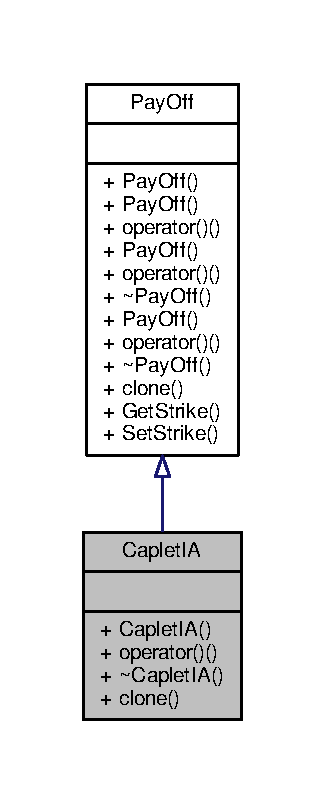
\includegraphics[width=156pt]{classCapletIA__inherit__graph}
\end{center}
\end{figure}


Collaboration diagram for Caplet\+IA\+:
\nopagebreak
\begin{figure}[H]
\begin{center}
\leavevmode
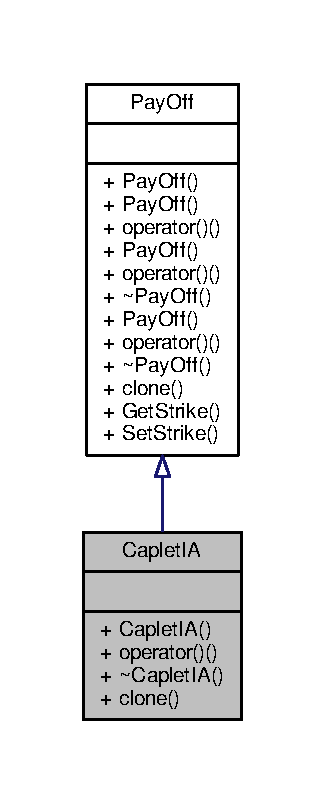
\includegraphics[width=156pt]{classCapletIA__coll__graph}
\end{center}
\end{figure}
\subsection*{Public Member Functions}
\begin{DoxyCompactItemize}
\item 
\hyperlink{classCapletIA_aa5244330f5862e096ad16103e2b85688}{Caplet\+IA} (double Strike\+\_\+, double t1\+\_\+, double t2\+\_\+)
\item 
virtual double \hyperlink{classCapletIA_a8dca8c52160a378ac2331ce95c688313}{operator()} (double Spot) const
\item 
virtual \hyperlink{classCapletIA_a05baa7e93ab0962a85520477dc820f51}{$\sim$\+Caplet\+IA} ()
\item 
virtual \hyperlink{classPayOff}{Pay\+Off} $\ast$ \hyperlink{classCapletIA_aebfbd05a398b551b43ac3118732934ba}{clone} () const
\end{DoxyCompactItemize}
\subsection*{Additional Inherited Members}


\subsection{Constructor \& Destructor Documentation}
\hypertarget{classCapletIA_aa5244330f5862e096ad16103e2b85688}{}\label{classCapletIA_aa5244330f5862e096ad16103e2b85688} 
\index{Caplet\+IA@{Caplet\+IA}!Caplet\+IA@{Caplet\+IA}}
\index{Caplet\+IA@{Caplet\+IA}!Caplet\+IA@{Caplet\+IA}}
\subsubsection{\texorpdfstring{Caplet\+I\+A()}{CapletIA()}}
{\footnotesize\ttfamily Caplet\+I\+A\+::\+Caplet\+IA (\begin{DoxyParamCaption}\item[{double}]{Strike\+\_\+,  }\item[{double}]{t1\+\_\+,  }\item[{double}]{t2\+\_\+ }\end{DoxyParamCaption})}

\hypertarget{classCapletIA_a05baa7e93ab0962a85520477dc820f51}{}\label{classCapletIA_a05baa7e93ab0962a85520477dc820f51} 
\index{Caplet\+IA@{Caplet\+IA}!````~Caplet\+IA@{$\sim$\+Caplet\+IA}}
\index{````~Caplet\+IA@{$\sim$\+Caplet\+IA}!Caplet\+IA@{Caplet\+IA}}
\subsubsection{\texorpdfstring{$\sim$\+Caplet\+I\+A()}{~CapletIA()}}
{\footnotesize\ttfamily virtual Caplet\+I\+A\+::$\sim$\+Caplet\+IA (\begin{DoxyParamCaption}{ }\end{DoxyParamCaption})\hspace{0.3cm}{\ttfamily [inline]}, {\ttfamily [virtual]}}



\subsection{Member Function Documentation}
\hypertarget{classCapletIA_aebfbd05a398b551b43ac3118732934ba}{}\label{classCapletIA_aebfbd05a398b551b43ac3118732934ba} 
\index{Caplet\+IA@{Caplet\+IA}!clone@{clone}}
\index{clone@{clone}!Caplet\+IA@{Caplet\+IA}}
\subsubsection{\texorpdfstring{clone()}{clone()}}
{\footnotesize\ttfamily virtual \hyperlink{classPayOff}{Pay\+Off}$\ast$ Caplet\+I\+A\+::clone (\begin{DoxyParamCaption}{ }\end{DoxyParamCaption}) const\hspace{0.3cm}{\ttfamily [virtual]}}



Implements \hyperlink{classPayOff_ad8194d5b82247ae89c25c515f0ba806a}{Pay\+Off}.

\hypertarget{classCapletIA_a8dca8c52160a378ac2331ce95c688313}{}\label{classCapletIA_a8dca8c52160a378ac2331ce95c688313} 
\index{Caplet\+IA@{Caplet\+IA}!operator()@{operator()}}
\index{operator()@{operator()}!Caplet\+IA@{Caplet\+IA}}
\subsubsection{\texorpdfstring{operator()()}{operator()()}}
{\footnotesize\ttfamily virtual double Caplet\+I\+A\+::operator() (\begin{DoxyParamCaption}\item[{double}]{Spot }\end{DoxyParamCaption}) const\hspace{0.3cm}{\ttfamily [virtual]}}



Implements \hyperlink{classPayOff_a5ae17d82c233ef5568c8fb0539703000}{Pay\+Off}.



The documentation for this class was generated from the following file\+:\begin{DoxyCompactItemize}
\item 
\hyperlink{payoff__interest__derivatives_8h}{payoff\+\_\+interest\+\_\+derivatives.\+h}\end{DoxyCompactItemize}

\hypertarget{classMyCashFlow_1_1CashFlow}{}\section{My\+Cash\+Flow\+:\+:Cash\+Flow Class Reference}
\label{classMyCashFlow_1_1CashFlow}\index{My\+Cash\+Flow\+::\+Cash\+Flow@{My\+Cash\+Flow\+::\+Cash\+Flow}}


{\ttfamily \#include $<$Path\+Dependent.\+h$>$}



Collaboration diagram for My\+Cash\+Flow\+:\+:Cash\+Flow\+:
\nopagebreak
\begin{figure}[H]
\begin{center}
\leavevmode
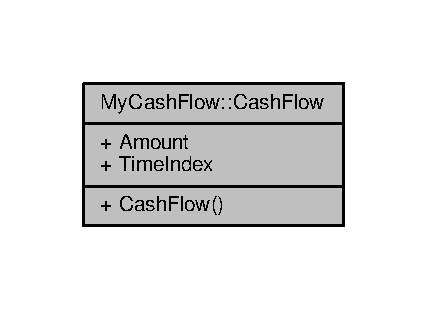
\includegraphics[width=205pt]{classMyCashFlow_1_1CashFlow__coll__graph}
\end{center}
\end{figure}
\subsection*{Public Member Functions}
\begin{DoxyCompactItemize}
\item 
\hyperlink{classMyCashFlow_1_1CashFlow_afa22922e78237519371139953975671c}{Cash\+Flow} (unsigned long Time\+Index\+\_\+=0\+U\+L, double Amount\+\_\+=0.\+0)
\end{DoxyCompactItemize}
\subsection*{Public Attributes}
\begin{DoxyCompactItemize}
\item 
double \hyperlink{classMyCashFlow_1_1CashFlow_ac6ddae0428eef4e3bb9b574e2fee077d}{Amount}
\item 
unsigned long \hyperlink{classMyCashFlow_1_1CashFlow_a6949eb507bf2de68eae7c60ed3cedbb7}{Time\+Index}
\end{DoxyCompactItemize}


\subsection{Constructor \& Destructor Documentation}
\hypertarget{classMyCashFlow_1_1CashFlow_afa22922e78237519371139953975671c}{}\label{classMyCashFlow_1_1CashFlow_afa22922e78237519371139953975671c} 
\index{My\+Cash\+Flow\+::\+Cash\+Flow@{My\+Cash\+Flow\+::\+Cash\+Flow}!Cash\+Flow@{Cash\+Flow}}
\index{Cash\+Flow@{Cash\+Flow}!My\+Cash\+Flow\+::\+Cash\+Flow@{My\+Cash\+Flow\+::\+Cash\+Flow}}
\subsubsection{\texorpdfstring{Cash\+Flow()}{CashFlow()}}
{\footnotesize\ttfamily My\+Cash\+Flow\+::\+Cash\+Flow\+::\+Cash\+Flow (\begin{DoxyParamCaption}\item[{unsigned long}]{Time\+Index\+\_\+ = {\ttfamily 0UL},  }\item[{double}]{Amount\+\_\+ = {\ttfamily 0.0} }\end{DoxyParamCaption})\hspace{0.3cm}{\ttfamily [inline]}}



\subsection{Member Data Documentation}
\hypertarget{classMyCashFlow_1_1CashFlow_ac6ddae0428eef4e3bb9b574e2fee077d}{}\label{classMyCashFlow_1_1CashFlow_ac6ddae0428eef4e3bb9b574e2fee077d} 
\index{My\+Cash\+Flow\+::\+Cash\+Flow@{My\+Cash\+Flow\+::\+Cash\+Flow}!Amount@{Amount}}
\index{Amount@{Amount}!My\+Cash\+Flow\+::\+Cash\+Flow@{My\+Cash\+Flow\+::\+Cash\+Flow}}
\subsubsection{\texorpdfstring{Amount}{Amount}}
{\footnotesize\ttfamily double My\+Cash\+Flow\+::\+Cash\+Flow\+::\+Amount}

\hypertarget{classMyCashFlow_1_1CashFlow_a6949eb507bf2de68eae7c60ed3cedbb7}{}\label{classMyCashFlow_1_1CashFlow_a6949eb507bf2de68eae7c60ed3cedbb7} 
\index{My\+Cash\+Flow\+::\+Cash\+Flow@{My\+Cash\+Flow\+::\+Cash\+Flow}!Time\+Index@{Time\+Index}}
\index{Time\+Index@{Time\+Index}!My\+Cash\+Flow\+::\+Cash\+Flow@{My\+Cash\+Flow\+::\+Cash\+Flow}}
\subsubsection{\texorpdfstring{Time\+Index}{TimeIndex}}
{\footnotesize\ttfamily unsigned long My\+Cash\+Flow\+::\+Cash\+Flow\+::\+Time\+Index}



The documentation for this class was generated from the following file\+:\begin{DoxyCompactItemize}
\item 
\hyperlink{PathDependent_8h}{Path\+Dependent.\+h}\end{DoxyCompactItemize}

\hypertarget{classConvergenceTable}{}\section{Convergence\+Table Class Reference}
\label{classConvergenceTable}\index{Convergence\+Table@{Convergence\+Table}}


{\ttfamily \#include $<$Convergence\+Table.\+h$>$}



Inheritance diagram for Convergence\+Table\+:
\nopagebreak
\begin{figure}[H]
\begin{center}
\leavevmode
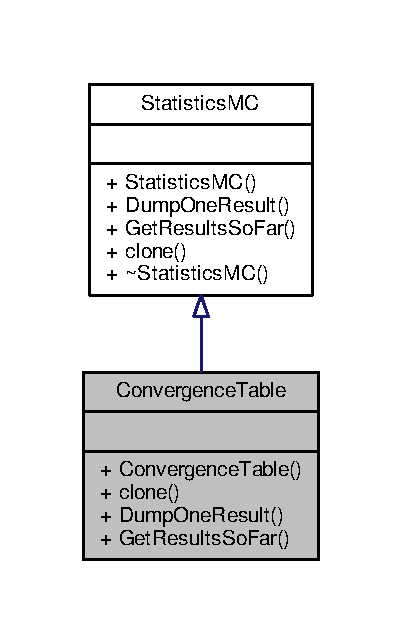
\includegraphics[width=193pt]{classConvergenceTable__inherit__graph}
\end{center}
\end{figure}


Collaboration diagram for Convergence\+Table\+:
\nopagebreak
\begin{figure}[H]
\begin{center}
\leavevmode
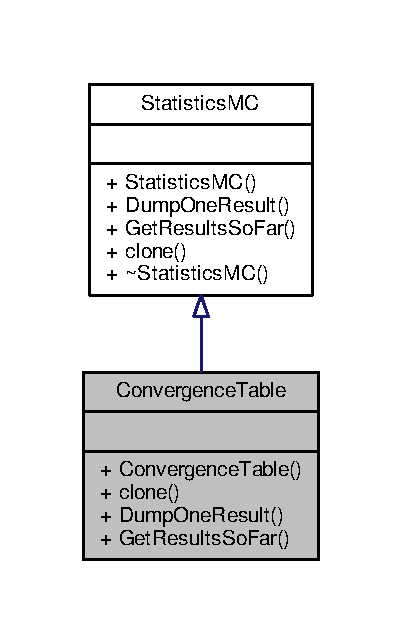
\includegraphics[width=193pt]{classConvergenceTable__coll__graph}
\end{center}
\end{figure}
\subsection*{Public Member Functions}
\begin{DoxyCompactItemize}
\item 
\hyperlink{classConvergenceTable_afcbd128680460340e121769f3cdc7e69}{Convergence\+Table} (const \hyperlink{classWrapper}{Wrapper}$<$ \hyperlink{classStatisticsMC}{Statistics\+MC} $>$ \&Inner\+\_\+)
\item 
virtual \hyperlink{classStatisticsMC}{Statistics\+MC} $\ast$ \hyperlink{classConvergenceTable_a129d95361fa2dd5a6ad43d4320f40682}{clone} () const
\item 
virtual void \hyperlink{classConvergenceTable_ae4ebb3988c6a8bc4e81049bfacf388e2}{Dump\+One\+Result} (double result)
\item 
virtual std\+::vector$<$ std\+::vector$<$ double $>$ $>$ \hyperlink{classConvergenceTable_a74d6d80fbfb1af7cd27ab306f0f619c0}{Get\+Results\+So\+Far} () const
\end{DoxyCompactItemize}


\subsection{Constructor \& Destructor Documentation}
\hypertarget{classConvergenceTable_afcbd128680460340e121769f3cdc7e69}{}\label{classConvergenceTable_afcbd128680460340e121769f3cdc7e69} 
\index{Convergence\+Table@{Convergence\+Table}!Convergence\+Table@{Convergence\+Table}}
\index{Convergence\+Table@{Convergence\+Table}!Convergence\+Table@{Convergence\+Table}}
\subsubsection{\texorpdfstring{Convergence\+Table()}{ConvergenceTable()}}
{\footnotesize\ttfamily Convergence\+Table\+::\+Convergence\+Table (\begin{DoxyParamCaption}\item[{const \hyperlink{classWrapper}{Wrapper}$<$ \hyperlink{classStatisticsMC}{Statistics\+MC} $>$ \&}]{Inner\+\_\+ }\end{DoxyParamCaption})}



\subsection{Member Function Documentation}
\hypertarget{classConvergenceTable_a129d95361fa2dd5a6ad43d4320f40682}{}\label{classConvergenceTable_a129d95361fa2dd5a6ad43d4320f40682} 
\index{Convergence\+Table@{Convergence\+Table}!clone@{clone}}
\index{clone@{clone}!Convergence\+Table@{Convergence\+Table}}
\subsubsection{\texorpdfstring{clone()}{clone()}}
{\footnotesize\ttfamily virtual \hyperlink{classStatisticsMC}{Statistics\+MC}$\ast$ Convergence\+Table\+::clone (\begin{DoxyParamCaption}{ }\end{DoxyParamCaption}) const\hspace{0.3cm}{\ttfamily [virtual]}}



Implements \hyperlink{classStatisticsMC_af716d17e088d36f283e112ba736f8002}{Statistics\+MC}.

\hypertarget{classConvergenceTable_ae4ebb3988c6a8bc4e81049bfacf388e2}{}\label{classConvergenceTable_ae4ebb3988c6a8bc4e81049bfacf388e2} 
\index{Convergence\+Table@{Convergence\+Table}!Dump\+One\+Result@{Dump\+One\+Result}}
\index{Dump\+One\+Result@{Dump\+One\+Result}!Convergence\+Table@{Convergence\+Table}}
\subsubsection{\texorpdfstring{Dump\+One\+Result()}{DumpOneResult()}}
{\footnotesize\ttfamily virtual void Convergence\+Table\+::\+Dump\+One\+Result (\begin{DoxyParamCaption}\item[{double}]{result }\end{DoxyParamCaption})\hspace{0.3cm}{\ttfamily [virtual]}}



Implements \hyperlink{classStatisticsMC_a3ab5fb27d6933d8e35b2a55c3897cbe3}{Statistics\+MC}.

\hypertarget{classConvergenceTable_a74d6d80fbfb1af7cd27ab306f0f619c0}{}\label{classConvergenceTable_a74d6d80fbfb1af7cd27ab306f0f619c0} 
\index{Convergence\+Table@{Convergence\+Table}!Get\+Results\+So\+Far@{Get\+Results\+So\+Far}}
\index{Get\+Results\+So\+Far@{Get\+Results\+So\+Far}!Convergence\+Table@{Convergence\+Table}}
\subsubsection{\texorpdfstring{Get\+Results\+So\+Far()}{GetResultsSoFar()}}
{\footnotesize\ttfamily virtual std\+::vector$<$std\+::vector$<$double$>$ $>$ Convergence\+Table\+::\+Get\+Results\+So\+Far (\begin{DoxyParamCaption}{ }\end{DoxyParamCaption}) const\hspace{0.3cm}{\ttfamily [virtual]}}



Implements \hyperlink{classStatisticsMC_ae29a294b6db36c2bf46c20ac30e25aad}{Statistics\+MC}.



The documentation for this class was generated from the following file\+:\begin{DoxyCompactItemize}
\item 
\hyperlink{ConvergenceTable_8h}{Convergence\+Table.\+h}\end{DoxyCompactItemize}

\hypertarget{classDeltaHedging}{}\section{Delta\+Hedging$<$ U $>$ Class Template Reference}
\label{classDeltaHedging}\index{Delta\+Hedging$<$ U $>$@{Delta\+Hedging$<$ U $>$}}


{\ttfamily \#include $<$hedging\+\_\+strategy.\+h$>$}



Inheritance diagram for Delta\+Hedging$<$ U $>$\+:
\nopagebreak
\begin{figure}[H]
\begin{center}
\leavevmode
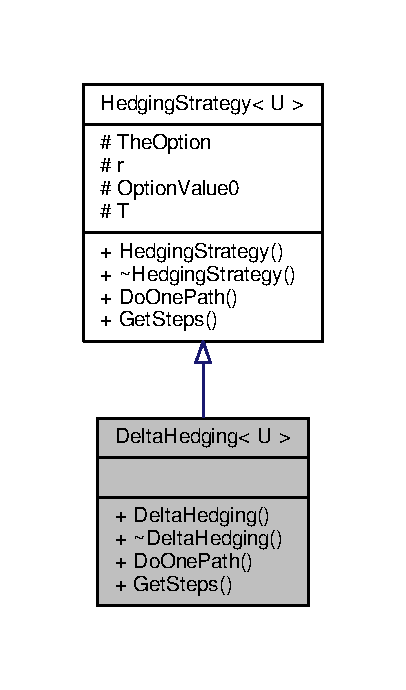
\includegraphics[width=195pt]{classDeltaHedging__inherit__graph}
\end{center}
\end{figure}


Collaboration diagram for Delta\+Hedging$<$ U $>$\+:
\nopagebreak
\begin{figure}[H]
\begin{center}
\leavevmode
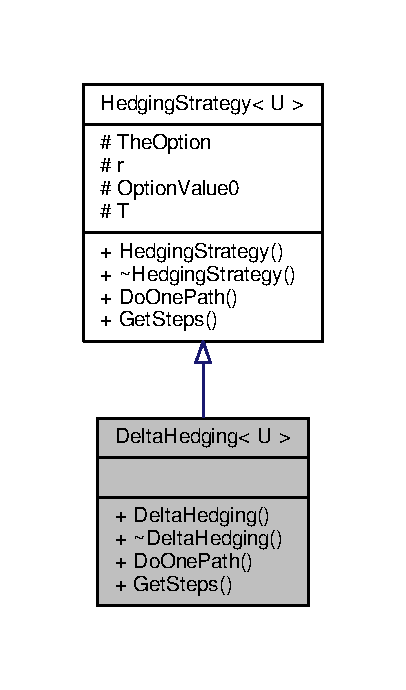
\includegraphics[width=195pt]{classDeltaHedging__coll__graph}
\end{center}
\end{figure}
\subsection*{Public Member Functions}
\begin{DoxyCompactItemize}
\item 
\hyperlink{classDeltaHedging_ae1e5687d0d2c9ba019e58cd2433fe81d}{Delta\+Hedging} (double \hyperlink{classHedgingStrategy_ac96528e9f4e5a0d1e5aadcc2ebdcab55}{Option\+Value0}, double \hyperlink{classHedgingStrategy_a313da7bc1911dba2a166d2c7bed5f1d7}{r}, shared\+\_\+ptr$<$ U $>$ \hyperlink{classHedgingStrategy_a65699a183423af9d947bb939ae8e907d}{The\+Option}, \hyperlink{classPathGenerationGBM}{Path\+Generation\+G\+BM} $\ast$The\+Path\+Generation, double \hyperlink{classHedgingStrategy_aedb4069f0709b49482a72b9d9c906a5e}{T})
\item 
virtual \hyperlink{classDeltaHedging_a019b8bef20aaec88a6e1e7bacb8c0015}{$\sim$\+Delta\+Hedging} ()
\item 
virtual double \hyperlink{classDeltaHedging_a670264651c7c2a3ce404bca291d2194f}{Do\+One\+Path} (\hyperlink{path__generation_8h_a75c13cde2074f502cc4348c70528572d}{args} \&args\+\_\+)
\item 
virtual unsigned long \hyperlink{classDeltaHedging_a0a6d6d2f73dfcf3425927cc45a012a2a}{Get\+Steps} () const
\end{DoxyCompactItemize}
\subsection*{Additional Inherited Members}


\subsection{Constructor \& Destructor Documentation}
\hypertarget{classDeltaHedging_ae1e5687d0d2c9ba019e58cd2433fe81d}{}\label{classDeltaHedging_ae1e5687d0d2c9ba019e58cd2433fe81d} 
\index{Delta\+Hedging@{Delta\+Hedging}!Delta\+Hedging@{Delta\+Hedging}}
\index{Delta\+Hedging@{Delta\+Hedging}!Delta\+Hedging@{Delta\+Hedging}}
\subsubsection{\texorpdfstring{Delta\+Hedging()}{DeltaHedging()}}
{\footnotesize\ttfamily template$<$typename U $>$ \\
\hyperlink{classDeltaHedging}{Delta\+Hedging}$<$ U $>$\+::\hyperlink{classDeltaHedging}{Delta\+Hedging} (\begin{DoxyParamCaption}\item[{double}]{Option\+Value0,  }\item[{double}]{r,  }\item[{shared\+\_\+ptr$<$ U $>$}]{The\+Option,  }\item[{\hyperlink{classPathGenerationGBM}{Path\+Generation\+G\+BM} $\ast$}]{The\+Path\+Generation,  }\item[{double}]{T }\end{DoxyParamCaption})}

\hypertarget{classDeltaHedging_a019b8bef20aaec88a6e1e7bacb8c0015}{}\label{classDeltaHedging_a019b8bef20aaec88a6e1e7bacb8c0015} 
\index{Delta\+Hedging@{Delta\+Hedging}!````~Delta\+Hedging@{$\sim$\+Delta\+Hedging}}
\index{````~Delta\+Hedging@{$\sim$\+Delta\+Hedging}!Delta\+Hedging@{Delta\+Hedging}}
\subsubsection{\texorpdfstring{$\sim$\+Delta\+Hedging()}{~DeltaHedging()}}
{\footnotesize\ttfamily template$<$typename U $>$ \\
virtual \hyperlink{classDeltaHedging}{Delta\+Hedging}$<$ U $>$\+::$\sim$\hyperlink{classDeltaHedging}{Delta\+Hedging} (\begin{DoxyParamCaption}{ }\end{DoxyParamCaption})\hspace{0.3cm}{\ttfamily [inline]}, {\ttfamily [virtual]}}



\subsection{Member Function Documentation}
\hypertarget{classDeltaHedging_a670264651c7c2a3ce404bca291d2194f}{}\label{classDeltaHedging_a670264651c7c2a3ce404bca291d2194f} 
\index{Delta\+Hedging@{Delta\+Hedging}!Do\+One\+Path@{Do\+One\+Path}}
\index{Do\+One\+Path@{Do\+One\+Path}!Delta\+Hedging@{Delta\+Hedging}}
\subsubsection{\texorpdfstring{Do\+One\+Path()}{DoOnePath()}}
{\footnotesize\ttfamily template$<$typename U $>$ \\
virtual double \hyperlink{classDeltaHedging}{Delta\+Hedging}$<$ U $>$\+::Do\+One\+Path (\begin{DoxyParamCaption}\item[{\hyperlink{path__generation_8h_a75c13cde2074f502cc4348c70528572d}{args} \&}]{args\+\_\+ }\end{DoxyParamCaption})\hspace{0.3cm}{\ttfamily [virtual]}}



Implements \hyperlink{classHedgingStrategy_ad2a7c02ee59750c40f29a03ee6fee140}{Hedging\+Strategy$<$ U $>$}.

\hypertarget{classDeltaHedging_a0a6d6d2f73dfcf3425927cc45a012a2a}{}\label{classDeltaHedging_a0a6d6d2f73dfcf3425927cc45a012a2a} 
\index{Delta\+Hedging@{Delta\+Hedging}!Get\+Steps@{Get\+Steps}}
\index{Get\+Steps@{Get\+Steps}!Delta\+Hedging@{Delta\+Hedging}}
\subsubsection{\texorpdfstring{Get\+Steps()}{GetSteps()}}
{\footnotesize\ttfamily template$<$typename U $>$ \\
virtual unsigned long \hyperlink{classDeltaHedging}{Delta\+Hedging}$<$ U $>$\+::Get\+Steps (\begin{DoxyParamCaption}{ }\end{DoxyParamCaption}) const\hspace{0.3cm}{\ttfamily [inline]}, {\ttfamily [virtual]}}



Implements \hyperlink{classHedgingStrategy_a4df1155158f019fb0c4f565045b9e633}{Hedging\+Strategy$<$ U $>$}.



The documentation for this class was generated from the following file\+:\begin{DoxyCompactItemize}
\item 
\hyperlink{hedging__strategy_8h}{hedging\+\_\+strategy.\+h}\end{DoxyCompactItemize}

\hypertarget{classDeltaHedgingCurrentVol}{}\section{Delta\+Hedging\+Current\+Vol$<$ U $>$ Class Template Reference}
\label{classDeltaHedgingCurrentVol}\index{Delta\+Hedging\+Current\+Vol$<$ U $>$@{Delta\+Hedging\+Current\+Vol$<$ U $>$}}


{\ttfamily \#include $<$hedging\+\_\+strategy\+\_\+sv.\+h$>$}



Inheritance diagram for Delta\+Hedging\+Current\+Vol$<$ U $>$\+:
\nopagebreak
\begin{figure}[H]
\begin{center}
\leavevmode
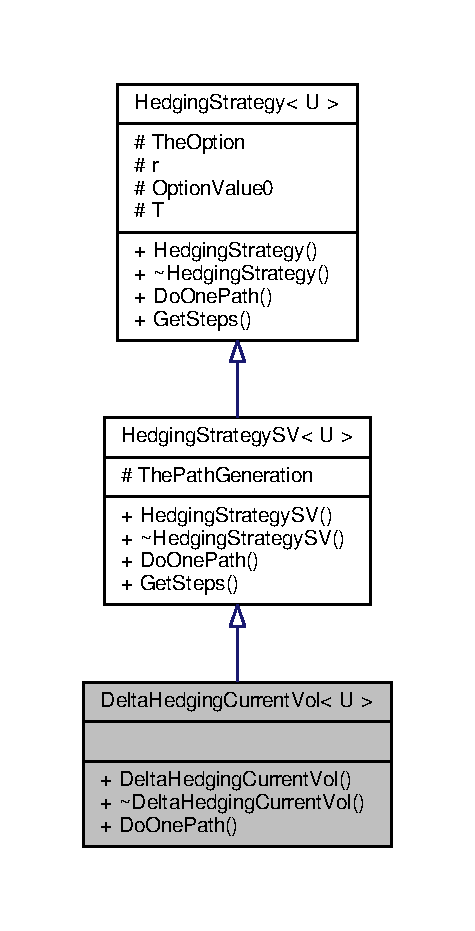
\includegraphics[width=228pt]{classDeltaHedgingCurrentVol__inherit__graph}
\end{center}
\end{figure}


Collaboration diagram for Delta\+Hedging\+Current\+Vol$<$ U $>$\+:
\nopagebreak
\begin{figure}[H]
\begin{center}
\leavevmode
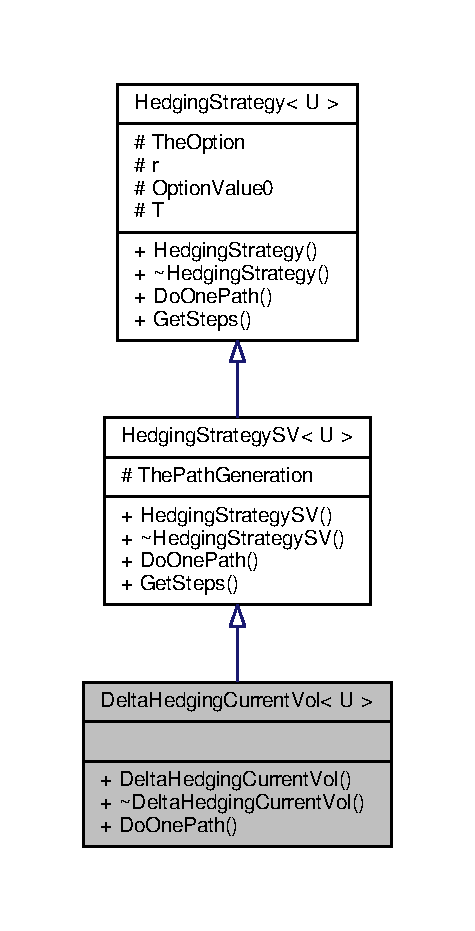
\includegraphics[width=228pt]{classDeltaHedgingCurrentVol__coll__graph}
\end{center}
\end{figure}
\subsection*{Public Member Functions}
\begin{DoxyCompactItemize}
\item 
\hyperlink{classDeltaHedgingCurrentVol_addf10fb5cc82a446b879da2951525a43}{Delta\+Hedging\+Current\+Vol} (double \hyperlink{classHedgingStrategy_ac96528e9f4e5a0d1e5aadcc2ebdcab55}{Option\+Value0}, double \hyperlink{classHedgingStrategy_a313da7bc1911dba2a166d2c7bed5f1d7}{r}, shared\+\_\+ptr$<$ U $>$ \hyperlink{classHedgingStrategy_a65699a183423af9d947bb939ae8e907d}{The\+Option}, shared\+\_\+ptr$<$ \hyperlink{classPathGenerationHeston}{Path\+Generation\+Heston} $>$ \hyperlink{classHedgingStrategySV_aa341650c5b2846606e59e3e6c6225aca}{The\+Path\+Generation}, double \hyperlink{classHedgingStrategy_aedb4069f0709b49482a72b9d9c906a5e}{T})
\item 
virtual \hyperlink{classDeltaHedgingCurrentVol_adcd16ce7b2d61e715167ee2ee94315ce}{$\sim$\+Delta\+Hedging\+Current\+Vol} ()
\item 
virtual double \hyperlink{classDeltaHedgingCurrentVol_ad235325f348bd58eb54d9dec389aa2e9}{Do\+One\+Path} (\hyperlink{path__generation_8h_a75c13cde2074f502cc4348c70528572d}{args} \&args\+\_\+)
\end{DoxyCompactItemize}
\subsection*{Additional Inherited Members}


\subsection{Constructor \& Destructor Documentation}
\hypertarget{classDeltaHedgingCurrentVol_addf10fb5cc82a446b879da2951525a43}{}\label{classDeltaHedgingCurrentVol_addf10fb5cc82a446b879da2951525a43} 
\index{Delta\+Hedging\+Current\+Vol@{Delta\+Hedging\+Current\+Vol}!Delta\+Hedging\+Current\+Vol@{Delta\+Hedging\+Current\+Vol}}
\index{Delta\+Hedging\+Current\+Vol@{Delta\+Hedging\+Current\+Vol}!Delta\+Hedging\+Current\+Vol@{Delta\+Hedging\+Current\+Vol}}
\subsubsection{\texorpdfstring{Delta\+Hedging\+Current\+Vol()}{DeltaHedgingCurrentVol()}}
{\footnotesize\ttfamily template$<$typename U $>$ \\
\hyperlink{classDeltaHedgingCurrentVol}{Delta\+Hedging\+Current\+Vol}$<$ U $>$\+::\hyperlink{classDeltaHedgingCurrentVol}{Delta\+Hedging\+Current\+Vol} (\begin{DoxyParamCaption}\item[{double}]{Option\+Value0,  }\item[{double}]{r,  }\item[{shared\+\_\+ptr$<$ U $>$}]{The\+Option,  }\item[{shared\+\_\+ptr$<$ \hyperlink{classPathGenerationHeston}{Path\+Generation\+Heston} $>$}]{The\+Path\+Generation,  }\item[{double}]{T }\end{DoxyParamCaption})}

\hypertarget{classDeltaHedgingCurrentVol_adcd16ce7b2d61e715167ee2ee94315ce}{}\label{classDeltaHedgingCurrentVol_adcd16ce7b2d61e715167ee2ee94315ce} 
\index{Delta\+Hedging\+Current\+Vol@{Delta\+Hedging\+Current\+Vol}!````~Delta\+Hedging\+Current\+Vol@{$\sim$\+Delta\+Hedging\+Current\+Vol}}
\index{````~Delta\+Hedging\+Current\+Vol@{$\sim$\+Delta\+Hedging\+Current\+Vol}!Delta\+Hedging\+Current\+Vol@{Delta\+Hedging\+Current\+Vol}}
\subsubsection{\texorpdfstring{$\sim$\+Delta\+Hedging\+Current\+Vol()}{~DeltaHedgingCurrentVol()}}
{\footnotesize\ttfamily template$<$typename U $>$ \\
virtual \hyperlink{classDeltaHedgingCurrentVol}{Delta\+Hedging\+Current\+Vol}$<$ U $>$\+::$\sim$\hyperlink{classDeltaHedgingCurrentVol}{Delta\+Hedging\+Current\+Vol} (\begin{DoxyParamCaption}{ }\end{DoxyParamCaption})\hspace{0.3cm}{\ttfamily [inline]}, {\ttfamily [virtual]}}



\subsection{Member Function Documentation}
\hypertarget{classDeltaHedgingCurrentVol_ad235325f348bd58eb54d9dec389aa2e9}{}\label{classDeltaHedgingCurrentVol_ad235325f348bd58eb54d9dec389aa2e9} 
\index{Delta\+Hedging\+Current\+Vol@{Delta\+Hedging\+Current\+Vol}!Do\+One\+Path@{Do\+One\+Path}}
\index{Do\+One\+Path@{Do\+One\+Path}!Delta\+Hedging\+Current\+Vol@{Delta\+Hedging\+Current\+Vol}}
\subsubsection{\texorpdfstring{Do\+One\+Path()}{DoOnePath()}}
{\footnotesize\ttfamily template$<$typename U $>$ \\
virtual double \hyperlink{classDeltaHedgingCurrentVol}{Delta\+Hedging\+Current\+Vol}$<$ U $>$\+::Do\+One\+Path (\begin{DoxyParamCaption}\item[{\hyperlink{path__generation_8h_a75c13cde2074f502cc4348c70528572d}{args} \&}]{args\+\_\+ }\end{DoxyParamCaption})\hspace{0.3cm}{\ttfamily [virtual]}}



Implements \hyperlink{classHedgingStrategySV_abb9531c069f4d1e758fc23c4bc7ed09c}{Hedging\+Strategy\+S\+V$<$ U $>$}.



The documentation for this class was generated from the following file\+:\begin{DoxyCompactItemize}
\item 
\hyperlink{hedging__strategy__sv_8h}{hedging\+\_\+strategy\+\_\+sv.\+h}\end{DoxyCompactItemize}

\hypertarget{classDeltaHedgingInstantVol}{}\section{Delta\+Hedging\+Instant\+Vol$<$ U $>$ Class Template Reference}
\label{classDeltaHedgingInstantVol}\index{Delta\+Hedging\+Instant\+Vol$<$ U $>$@{Delta\+Hedging\+Instant\+Vol$<$ U $>$}}


{\ttfamily \#include $<$hedging\+\_\+strategy\+\_\+sv.\+h$>$}



Inheritance diagram for Delta\+Hedging\+Instant\+Vol$<$ U $>$\+:
\nopagebreak
\begin{figure}[H]
\begin{center}
\leavevmode
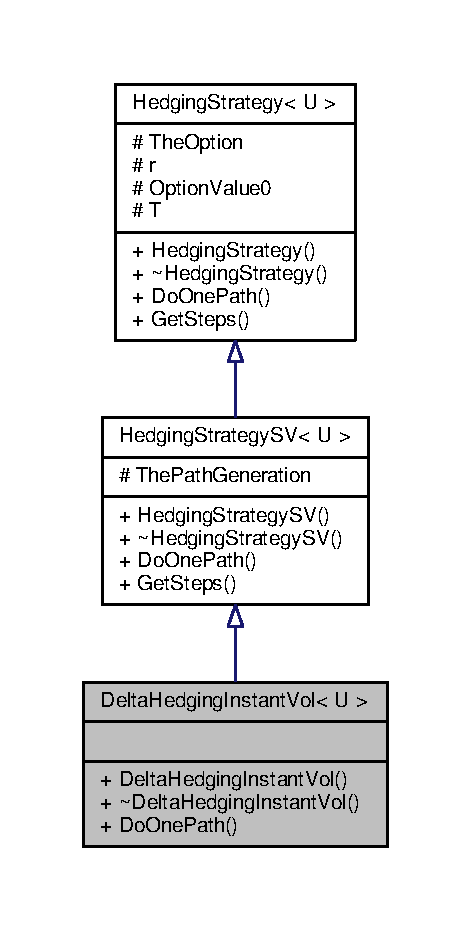
\includegraphics[width=226pt]{classDeltaHedgingInstantVol__inherit__graph}
\end{center}
\end{figure}


Collaboration diagram for Delta\+Hedging\+Instant\+Vol$<$ U $>$\+:
\nopagebreak
\begin{figure}[H]
\begin{center}
\leavevmode
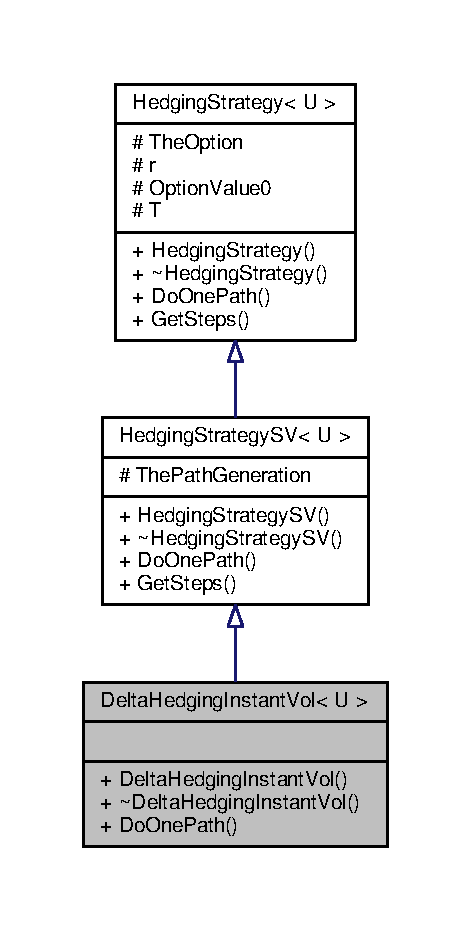
\includegraphics[width=226pt]{classDeltaHedgingInstantVol__coll__graph}
\end{center}
\end{figure}
\subsection*{Public Member Functions}
\begin{DoxyCompactItemize}
\item 
\hyperlink{classDeltaHedgingInstantVol_a64229bc4a65fa32959d22bc449ad0520}{Delta\+Hedging\+Instant\+Vol} (double \hyperlink{classHedgingStrategy_ac96528e9f4e5a0d1e5aadcc2ebdcab55}{Option\+Value0}, double \hyperlink{classHedgingStrategy_a313da7bc1911dba2a166d2c7bed5f1d7}{r}, shared\+\_\+ptr$<$ U $>$ \hyperlink{classHedgingStrategy_a65699a183423af9d947bb939ae8e907d}{The\+Option}, shared\+\_\+ptr$<$ \hyperlink{classPathGenerationHeston}{Path\+Generation\+Heston} $>$ \hyperlink{classHedgingStrategySV_aa341650c5b2846606e59e3e6c6225aca}{The\+Path\+Generation}, double \hyperlink{classHedgingStrategy_aedb4069f0709b49482a72b9d9c906a5e}{T})
\item 
virtual \hyperlink{classDeltaHedgingInstantVol_a87a3e73ee61d8dc3d9d04120f9f323a3}{$\sim$\+Delta\+Hedging\+Instant\+Vol} ()
\item 
virtual double \hyperlink{classDeltaHedgingInstantVol_ac05386c300db720ed07d8465123a8f7a}{Do\+One\+Path} (\hyperlink{path__generation_8h_a75c13cde2074f502cc4348c70528572d}{args} \&args\+\_\+)
\end{DoxyCompactItemize}
\subsection*{Additional Inherited Members}


\subsection{Constructor \& Destructor Documentation}
\hypertarget{classDeltaHedgingInstantVol_a64229bc4a65fa32959d22bc449ad0520}{}\label{classDeltaHedgingInstantVol_a64229bc4a65fa32959d22bc449ad0520} 
\index{Delta\+Hedging\+Instant\+Vol@{Delta\+Hedging\+Instant\+Vol}!Delta\+Hedging\+Instant\+Vol@{Delta\+Hedging\+Instant\+Vol}}
\index{Delta\+Hedging\+Instant\+Vol@{Delta\+Hedging\+Instant\+Vol}!Delta\+Hedging\+Instant\+Vol@{Delta\+Hedging\+Instant\+Vol}}
\subsubsection{\texorpdfstring{Delta\+Hedging\+Instant\+Vol()}{DeltaHedgingInstantVol()}}
{\footnotesize\ttfamily template$<$typename U $>$ \\
\hyperlink{classDeltaHedgingInstantVol}{Delta\+Hedging\+Instant\+Vol}$<$ U $>$\+::\hyperlink{classDeltaHedgingInstantVol}{Delta\+Hedging\+Instant\+Vol} (\begin{DoxyParamCaption}\item[{double}]{Option\+Value0,  }\item[{double}]{r,  }\item[{shared\+\_\+ptr$<$ U $>$}]{The\+Option,  }\item[{shared\+\_\+ptr$<$ \hyperlink{classPathGenerationHeston}{Path\+Generation\+Heston} $>$}]{The\+Path\+Generation,  }\item[{double}]{T }\end{DoxyParamCaption})}

\hypertarget{classDeltaHedgingInstantVol_a87a3e73ee61d8dc3d9d04120f9f323a3}{}\label{classDeltaHedgingInstantVol_a87a3e73ee61d8dc3d9d04120f9f323a3} 
\index{Delta\+Hedging\+Instant\+Vol@{Delta\+Hedging\+Instant\+Vol}!````~Delta\+Hedging\+Instant\+Vol@{$\sim$\+Delta\+Hedging\+Instant\+Vol}}
\index{````~Delta\+Hedging\+Instant\+Vol@{$\sim$\+Delta\+Hedging\+Instant\+Vol}!Delta\+Hedging\+Instant\+Vol@{Delta\+Hedging\+Instant\+Vol}}
\subsubsection{\texorpdfstring{$\sim$\+Delta\+Hedging\+Instant\+Vol()}{~DeltaHedgingInstantVol()}}
{\footnotesize\ttfamily template$<$typename U $>$ \\
virtual \hyperlink{classDeltaHedgingInstantVol}{Delta\+Hedging\+Instant\+Vol}$<$ U $>$\+::$\sim$\hyperlink{classDeltaHedgingInstantVol}{Delta\+Hedging\+Instant\+Vol} (\begin{DoxyParamCaption}{ }\end{DoxyParamCaption})\hspace{0.3cm}{\ttfamily [inline]}, {\ttfamily [virtual]}}



\subsection{Member Function Documentation}
\hypertarget{classDeltaHedgingInstantVol_ac05386c300db720ed07d8465123a8f7a}{}\label{classDeltaHedgingInstantVol_ac05386c300db720ed07d8465123a8f7a} 
\index{Delta\+Hedging\+Instant\+Vol@{Delta\+Hedging\+Instant\+Vol}!Do\+One\+Path@{Do\+One\+Path}}
\index{Do\+One\+Path@{Do\+One\+Path}!Delta\+Hedging\+Instant\+Vol@{Delta\+Hedging\+Instant\+Vol}}
\subsubsection{\texorpdfstring{Do\+One\+Path()}{DoOnePath()}}
{\footnotesize\ttfamily template$<$typename U $>$ \\
virtual double \hyperlink{classDeltaHedgingInstantVol}{Delta\+Hedging\+Instant\+Vol}$<$ U $>$\+::Do\+One\+Path (\begin{DoxyParamCaption}\item[{\hyperlink{path__generation_8h_a75c13cde2074f502cc4348c70528572d}{args} \&}]{args\+\_\+ }\end{DoxyParamCaption})\hspace{0.3cm}{\ttfamily [virtual]}}



Implements \hyperlink{classHedgingStrategySV_abb9531c069f4d1e758fc23c4bc7ed09c}{Hedging\+Strategy\+S\+V$<$ U $>$}.



The documentation for this class was generated from the following file\+:\begin{DoxyCompactItemize}
\item 
\hyperlink{hedging__strategy__sv_8h}{hedging\+\_\+strategy\+\_\+sv.\+h}\end{DoxyCompactItemize}

\hypertarget{classDeltaHedgingRMS}{}\section{Delta\+Hedging\+R\+MS$<$ U $>$ Class Template Reference}
\label{classDeltaHedgingRMS}\index{Delta\+Hedging\+R\+M\+S$<$ U $>$@{Delta\+Hedging\+R\+M\+S$<$ U $>$}}


{\ttfamily \#include $<$hedging\+\_\+strategy\+\_\+sv.\+h$>$}



Inheritance diagram for Delta\+Hedging\+R\+MS$<$ U $>$\+:
\nopagebreak
\begin{figure}[H]
\begin{center}
\leavevmode
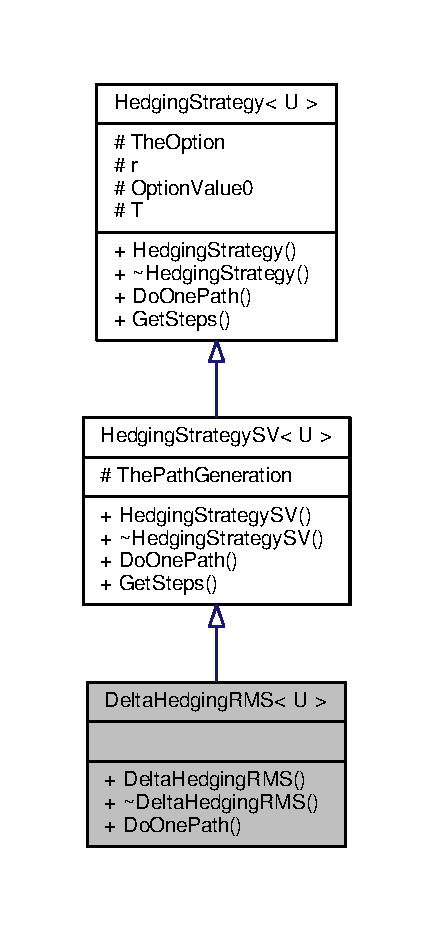
\includegraphics[width=208pt]{classDeltaHedgingRMS__inherit__graph}
\end{center}
\end{figure}


Collaboration diagram for Delta\+Hedging\+R\+MS$<$ U $>$\+:
\nopagebreak
\begin{figure}[H]
\begin{center}
\leavevmode
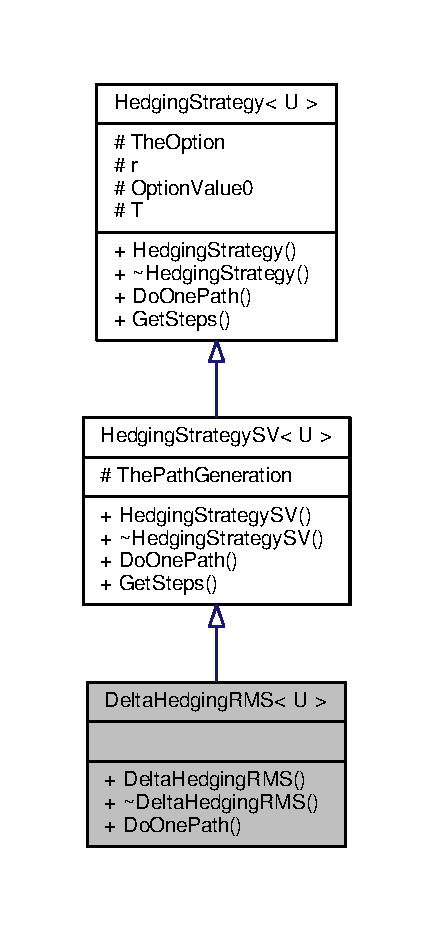
\includegraphics[width=208pt]{classDeltaHedgingRMS__coll__graph}
\end{center}
\end{figure}
\subsection*{Public Member Functions}
\begin{DoxyCompactItemize}
\item 
\hyperlink{classDeltaHedgingRMS_a5b31d762316b99c787328394d28d90a0}{Delta\+Hedging\+R\+MS} (double \hyperlink{classHedgingStrategy_ac96528e9f4e5a0d1e5aadcc2ebdcab55}{Option\+Value0}, double \hyperlink{classHedgingStrategy_a313da7bc1911dba2a166d2c7bed5f1d7}{r}, shared\+\_\+ptr$<$ U $>$ \hyperlink{classHedgingStrategy_a65699a183423af9d947bb939ae8e907d}{The\+Option}, shared\+\_\+ptr$<$ \hyperlink{classPathGenerationHeston}{Path\+Generation\+Heston} $>$ \hyperlink{classHedgingStrategySV_aa341650c5b2846606e59e3e6c6225aca}{The\+Path\+Generation}, double \hyperlink{classHedgingStrategy_aedb4069f0709b49482a72b9d9c906a5e}{T})
\item 
virtual \hyperlink{classDeltaHedgingRMS_a5d94af75ab8235dd533b5225ce7964e1}{$\sim$\+Delta\+Hedging\+R\+MS} ()
\item 
virtual double \hyperlink{classDeltaHedgingRMS_ad1dfe5625f1064b9b1f8a45b20f0ee50}{Do\+One\+Path} (\hyperlink{path__generation_8h_a75c13cde2074f502cc4348c70528572d}{args} \&args\+\_\+)
\end{DoxyCompactItemize}
\subsection*{Additional Inherited Members}


\subsection{Constructor \& Destructor Documentation}
\hypertarget{classDeltaHedgingRMS_a5b31d762316b99c787328394d28d90a0}{}\label{classDeltaHedgingRMS_a5b31d762316b99c787328394d28d90a0} 
\index{Delta\+Hedging\+R\+MS@{Delta\+Hedging\+R\+MS}!Delta\+Hedging\+R\+MS@{Delta\+Hedging\+R\+MS}}
\index{Delta\+Hedging\+R\+MS@{Delta\+Hedging\+R\+MS}!Delta\+Hedging\+R\+MS@{Delta\+Hedging\+R\+MS}}
\subsubsection{\texorpdfstring{Delta\+Hedging\+R\+M\+S()}{DeltaHedgingRMS()}}
{\footnotesize\ttfamily template$<$typename U $>$ \\
\hyperlink{classDeltaHedgingRMS}{Delta\+Hedging\+R\+MS}$<$ U $>$\+::\hyperlink{classDeltaHedgingRMS}{Delta\+Hedging\+R\+MS} (\begin{DoxyParamCaption}\item[{double}]{Option\+Value0,  }\item[{double}]{r,  }\item[{shared\+\_\+ptr$<$ U $>$}]{The\+Option,  }\item[{shared\+\_\+ptr$<$ \hyperlink{classPathGenerationHeston}{Path\+Generation\+Heston} $>$}]{The\+Path\+Generation,  }\item[{double}]{T }\end{DoxyParamCaption})}

\hypertarget{classDeltaHedgingRMS_a5d94af75ab8235dd533b5225ce7964e1}{}\label{classDeltaHedgingRMS_a5d94af75ab8235dd533b5225ce7964e1} 
\index{Delta\+Hedging\+R\+MS@{Delta\+Hedging\+R\+MS}!````~Delta\+Hedging\+R\+MS@{$\sim$\+Delta\+Hedging\+R\+MS}}
\index{````~Delta\+Hedging\+R\+MS@{$\sim$\+Delta\+Hedging\+R\+MS}!Delta\+Hedging\+R\+MS@{Delta\+Hedging\+R\+MS}}
\subsubsection{\texorpdfstring{$\sim$\+Delta\+Hedging\+R\+M\+S()}{~DeltaHedgingRMS()}}
{\footnotesize\ttfamily template$<$typename U $>$ \\
virtual \hyperlink{classDeltaHedgingRMS}{Delta\+Hedging\+R\+MS}$<$ U $>$\+::$\sim$\hyperlink{classDeltaHedgingRMS}{Delta\+Hedging\+R\+MS} (\begin{DoxyParamCaption}{ }\end{DoxyParamCaption})\hspace{0.3cm}{\ttfamily [inline]}, {\ttfamily [virtual]}}



\subsection{Member Function Documentation}
\hypertarget{classDeltaHedgingRMS_ad1dfe5625f1064b9b1f8a45b20f0ee50}{}\label{classDeltaHedgingRMS_ad1dfe5625f1064b9b1f8a45b20f0ee50} 
\index{Delta\+Hedging\+R\+MS@{Delta\+Hedging\+R\+MS}!Do\+One\+Path@{Do\+One\+Path}}
\index{Do\+One\+Path@{Do\+One\+Path}!Delta\+Hedging\+R\+MS@{Delta\+Hedging\+R\+MS}}
\subsubsection{\texorpdfstring{Do\+One\+Path()}{DoOnePath()}}
{\footnotesize\ttfamily template$<$typename U $>$ \\
virtual double \hyperlink{classDeltaHedgingRMS}{Delta\+Hedging\+R\+MS}$<$ U $>$\+::Do\+One\+Path (\begin{DoxyParamCaption}\item[{\hyperlink{path__generation_8h_a75c13cde2074f502cc4348c70528572d}{args} \&}]{args\+\_\+ }\end{DoxyParamCaption})\hspace{0.3cm}{\ttfamily [virtual]}}



Implements \hyperlink{classHedgingStrategySV_abb9531c069f4d1e758fc23c4bc7ed09c}{Hedging\+Strategy\+S\+V$<$ U $>$}.



The documentation for this class was generated from the following file\+:\begin{DoxyCompactItemize}
\item 
\hyperlink{hedging__strategy__sv_8h}{hedging\+\_\+strategy\+\_\+sv.\+h}\end{DoxyCompactItemize}

\hypertarget{classDeltaHedgingRMSDec}{}\section{Delta\+Hedging\+R\+M\+S\+Dec$<$ U $>$ Class Template Reference}
\label{classDeltaHedgingRMSDec}\index{Delta\+Hedging\+R\+M\+S\+Dec$<$ U $>$@{Delta\+Hedging\+R\+M\+S\+Dec$<$ U $>$}}


{\ttfamily \#include $<$hedging\+\_\+strategy\+\_\+sv.\+h$>$}



Inheritance diagram for Delta\+Hedging\+R\+M\+S\+Dec$<$ U $>$\+:
\nopagebreak
\begin{figure}[H]
\begin{center}
\leavevmode
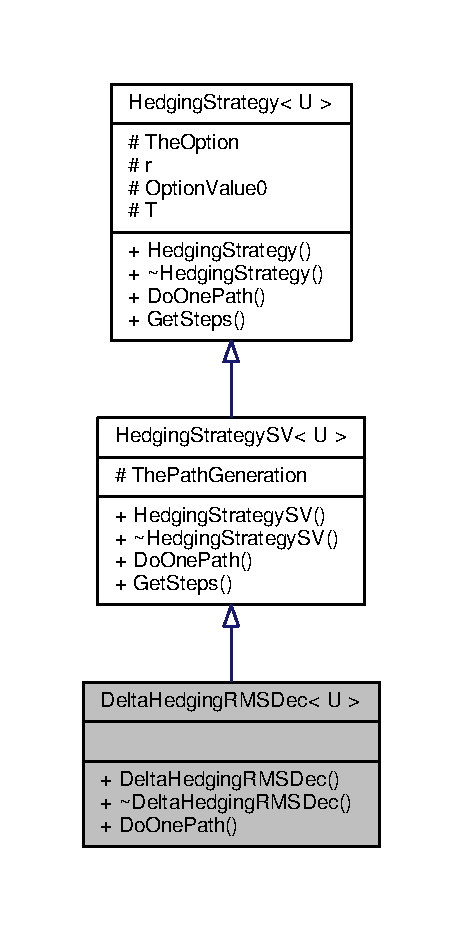
\includegraphics[width=222pt]{classDeltaHedgingRMSDec__inherit__graph}
\end{center}
\end{figure}


Collaboration diagram for Delta\+Hedging\+R\+M\+S\+Dec$<$ U $>$\+:
\nopagebreak
\begin{figure}[H]
\begin{center}
\leavevmode
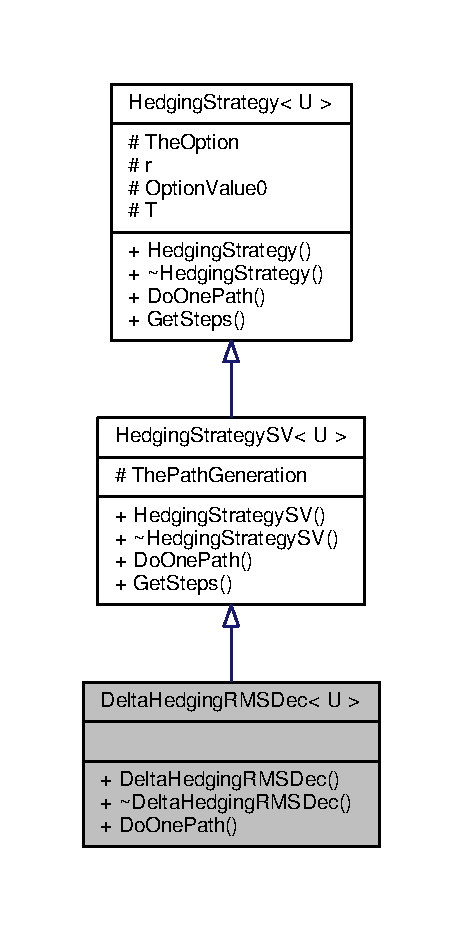
\includegraphics[width=222pt]{classDeltaHedgingRMSDec__coll__graph}
\end{center}
\end{figure}
\subsection*{Public Member Functions}
\begin{DoxyCompactItemize}
\item 
\hyperlink{classDeltaHedgingRMSDec_a47c0fd66e96b5c75dfc999883e4124d3}{Delta\+Hedging\+R\+M\+S\+Dec} (double \hyperlink{classHedgingStrategy_ac96528e9f4e5a0d1e5aadcc2ebdcab55}{Option\+Value0}, double \hyperlink{classHedgingStrategy_a313da7bc1911dba2a166d2c7bed5f1d7}{r}, shared\+\_\+ptr$<$ U $>$ \hyperlink{classHedgingStrategy_a65699a183423af9d947bb939ae8e907d}{The\+Option}, shared\+\_\+ptr$<$ \hyperlink{classPathGenerationHeston}{Path\+Generation\+Heston} $>$ \hyperlink{classHedgingStrategySV_aa341650c5b2846606e59e3e6c6225aca}{The\+Path\+Generation}, double \hyperlink{classHedgingStrategy_aedb4069f0709b49482a72b9d9c906a5e}{T})
\item 
virtual \hyperlink{classDeltaHedgingRMSDec_ac01f0ab7f61f34e2d02b2be0a4f109c0}{$\sim$\+Delta\+Hedging\+R\+M\+S\+Dec} ()
\item 
virtual double \hyperlink{classDeltaHedgingRMSDec_aa9118ce56921178e38a7ed8a6acee656}{Do\+One\+Path} (\hyperlink{path__generation_8h_a75c13cde2074f502cc4348c70528572d}{args} \&args\+\_\+)
\end{DoxyCompactItemize}
\subsection*{Additional Inherited Members}


\subsection{Constructor \& Destructor Documentation}
\hypertarget{classDeltaHedgingRMSDec_a47c0fd66e96b5c75dfc999883e4124d3}{}\label{classDeltaHedgingRMSDec_a47c0fd66e96b5c75dfc999883e4124d3} 
\index{Delta\+Hedging\+R\+M\+S\+Dec@{Delta\+Hedging\+R\+M\+S\+Dec}!Delta\+Hedging\+R\+M\+S\+Dec@{Delta\+Hedging\+R\+M\+S\+Dec}}
\index{Delta\+Hedging\+R\+M\+S\+Dec@{Delta\+Hedging\+R\+M\+S\+Dec}!Delta\+Hedging\+R\+M\+S\+Dec@{Delta\+Hedging\+R\+M\+S\+Dec}}
\subsubsection{\texorpdfstring{Delta\+Hedging\+R\+M\+S\+Dec()}{DeltaHedgingRMSDec()}}
{\footnotesize\ttfamily template$<$typename U $>$ \\
\hyperlink{classDeltaHedgingRMSDec}{Delta\+Hedging\+R\+M\+S\+Dec}$<$ U $>$\+::\hyperlink{classDeltaHedgingRMSDec}{Delta\+Hedging\+R\+M\+S\+Dec} (\begin{DoxyParamCaption}\item[{double}]{Option\+Value0,  }\item[{double}]{r,  }\item[{shared\+\_\+ptr$<$ U $>$}]{The\+Option,  }\item[{shared\+\_\+ptr$<$ \hyperlink{classPathGenerationHeston}{Path\+Generation\+Heston} $>$}]{The\+Path\+Generation,  }\item[{double}]{T }\end{DoxyParamCaption})}

\hypertarget{classDeltaHedgingRMSDec_ac01f0ab7f61f34e2d02b2be0a4f109c0}{}\label{classDeltaHedgingRMSDec_ac01f0ab7f61f34e2d02b2be0a4f109c0} 
\index{Delta\+Hedging\+R\+M\+S\+Dec@{Delta\+Hedging\+R\+M\+S\+Dec}!````~Delta\+Hedging\+R\+M\+S\+Dec@{$\sim$\+Delta\+Hedging\+R\+M\+S\+Dec}}
\index{````~Delta\+Hedging\+R\+M\+S\+Dec@{$\sim$\+Delta\+Hedging\+R\+M\+S\+Dec}!Delta\+Hedging\+R\+M\+S\+Dec@{Delta\+Hedging\+R\+M\+S\+Dec}}
\subsubsection{\texorpdfstring{$\sim$\+Delta\+Hedging\+R\+M\+S\+Dec()}{~DeltaHedgingRMSDec()}}
{\footnotesize\ttfamily template$<$typename U $>$ \\
virtual \hyperlink{classDeltaHedgingRMSDec}{Delta\+Hedging\+R\+M\+S\+Dec}$<$ U $>$\+::$\sim$\hyperlink{classDeltaHedgingRMSDec}{Delta\+Hedging\+R\+M\+S\+Dec} (\begin{DoxyParamCaption}{ }\end{DoxyParamCaption})\hspace{0.3cm}{\ttfamily [inline]}, {\ttfamily [virtual]}}



\subsection{Member Function Documentation}
\hypertarget{classDeltaHedgingRMSDec_aa9118ce56921178e38a7ed8a6acee656}{}\label{classDeltaHedgingRMSDec_aa9118ce56921178e38a7ed8a6acee656} 
\index{Delta\+Hedging\+R\+M\+S\+Dec@{Delta\+Hedging\+R\+M\+S\+Dec}!Do\+One\+Path@{Do\+One\+Path}}
\index{Do\+One\+Path@{Do\+One\+Path}!Delta\+Hedging\+R\+M\+S\+Dec@{Delta\+Hedging\+R\+M\+S\+Dec}}
\subsubsection{\texorpdfstring{Do\+One\+Path()}{DoOnePath()}}
{\footnotesize\ttfamily template$<$typename U $>$ \\
virtual double \hyperlink{classDeltaHedgingRMSDec}{Delta\+Hedging\+R\+M\+S\+Dec}$<$ U $>$\+::Do\+One\+Path (\begin{DoxyParamCaption}\item[{\hyperlink{path__generation_8h_a75c13cde2074f502cc4348c70528572d}{args} \&}]{args\+\_\+ }\end{DoxyParamCaption})\hspace{0.3cm}{\ttfamily [virtual]}}



Implements \hyperlink{classHedgingStrategySV_abb9531c069f4d1e758fc23c4bc7ed09c}{Hedging\+Strategy\+S\+V$<$ U $>$}.



The documentation for this class was generated from the following file\+:\begin{DoxyCompactItemize}
\item 
\hyperlink{hedging__strategy__sv_8h}{hedging\+\_\+strategy\+\_\+sv.\+h}\end{DoxyCompactItemize}

\hypertarget{classMyOption_1_1DigitalCallOption}{}\section{My\+Option\+:\+:Digital\+Call\+Option Class Reference}
\label{classMyOption_1_1DigitalCallOption}\index{My\+Option\+::\+Digital\+Call\+Option@{My\+Option\+::\+Digital\+Call\+Option}}


{\ttfamily \#include $<$options.\+h$>$}



Inheritance diagram for My\+Option\+:\+:Digital\+Call\+Option\+:
\nopagebreak
\begin{figure}[H]
\begin{center}
\leavevmode
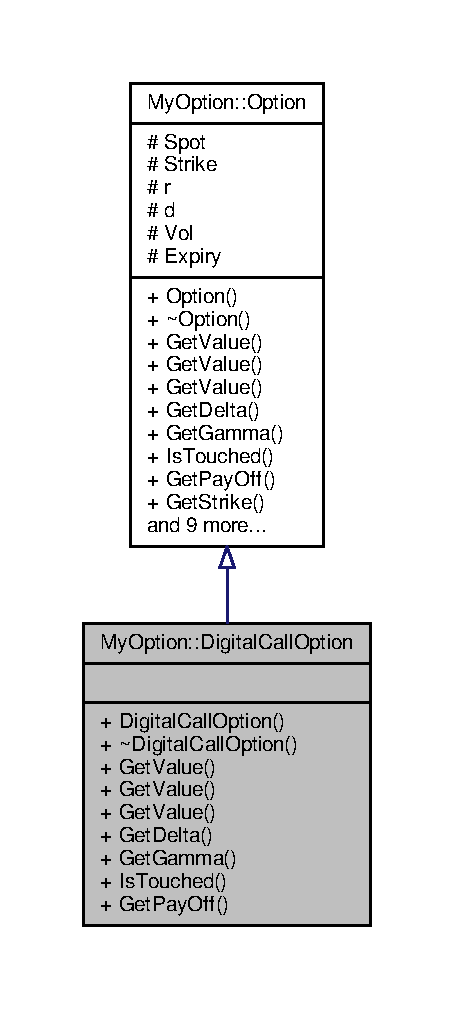
\includegraphics[width=218pt]{classMyOption_1_1DigitalCallOption__inherit__graph}
\end{center}
\end{figure}


Collaboration diagram for My\+Option\+:\+:Digital\+Call\+Option\+:
\nopagebreak
\begin{figure}[H]
\begin{center}
\leavevmode
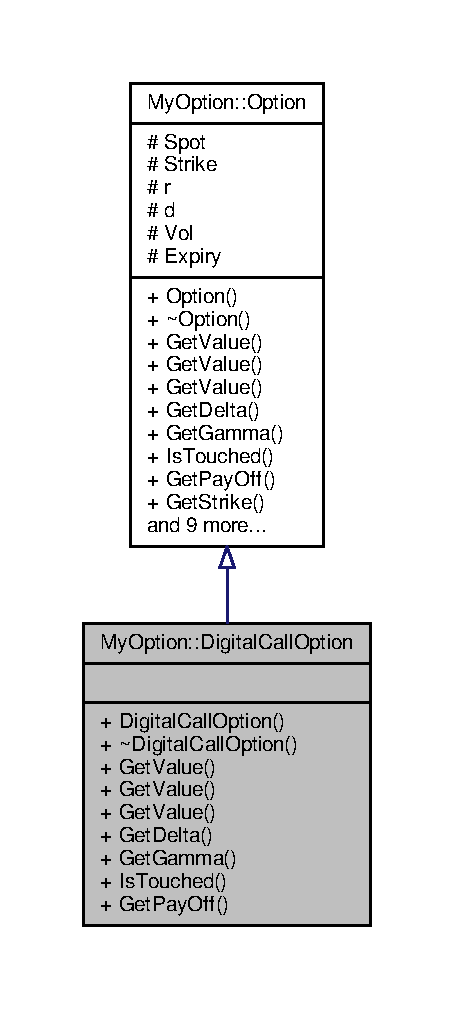
\includegraphics[width=218pt]{classMyOption_1_1DigitalCallOption__coll__graph}
\end{center}
\end{figure}
\subsection*{Public Member Functions}
\begin{DoxyCompactItemize}
\item 
\hyperlink{classMyOption_1_1DigitalCallOption_ab09ac328d7fe9da0ba735c36e9929ad5}{Digital\+Call\+Option} (double \hyperlink{classMyOption_1_1Option_a6c6f01d75cde7e92d16a6d8d6f331a1d}{Spot}, double \hyperlink{classMyOption_1_1Option_a3033c483588ce26b175280c7f9dee8d1}{Strike}, double \hyperlink{classMyOption_1_1Option_aa8cb250427dece65ea49255d4102cc8d}{r}, double \hyperlink{classMyOption_1_1Option_a500979f4b32262594d895c4a83b58d1d}{d}, double \hyperlink{classMyOption_1_1Option_a5d6002c14b335c782873bf1437113513}{Vol}, double \hyperlink{classMyOption_1_1Option_ac1adacb417fede41d151b9cda05bcb3d}{Expiry})
\item 
virtual \hyperlink{classMyOption_1_1DigitalCallOption_acc2d14a2b95f2a43ee8a09b39591a071}{$\sim$\+Digital\+Call\+Option} ()
\item 
virtual double \hyperlink{classMyOption_1_1DigitalCallOption_a9c05c136304f5b2112ed87859c5a944a}{Get\+Value} (double \hyperlink{classMyOption_1_1Option_a6c6f01d75cde7e92d16a6d8d6f331a1d}{Spot})
\item 
virtual double \hyperlink{classMyOption_1_1DigitalCallOption_a353ecc50b8e9efa5c4c2cc06454760b6}{Get\+Value} (double \hyperlink{classMyOption_1_1Option_a6c6f01d75cde7e92d16a6d8d6f331a1d}{Spot}, double \hyperlink{classMyOption_1_1Option_a5d6002c14b335c782873bf1437113513}{Vol}, double \hyperlink{classMyOption_1_1Option_ac1adacb417fede41d151b9cda05bcb3d}{Expiry})
\item 
virtual double \hyperlink{classMyOption_1_1DigitalCallOption_a75391ad8c6b599e0c181c965d01cd610}{Get\+Value} (double \hyperlink{classMyOption_1_1Option_a6c6f01d75cde7e92d16a6d8d6f331a1d}{Spot}, double \hyperlink{classMyOption_1_1Option_aa8cb250427dece65ea49255d4102cc8d}{r}, double \hyperlink{classMyOption_1_1Option_a5d6002c14b335c782873bf1437113513}{Vol}, double \hyperlink{classMyOption_1_1Option_ac1adacb417fede41d151b9cda05bcb3d}{Expiry})
\item 
virtual double \hyperlink{classMyOption_1_1DigitalCallOption_a58446219e938256d1f451930350737b7}{Get\+Delta} (double \hyperlink{classMyOption_1_1Option_a6c6f01d75cde7e92d16a6d8d6f331a1d}{Spot}, double \hyperlink{classMyOption_1_1Option_a5d6002c14b335c782873bf1437113513}{Vol}, double \hyperlink{classMyOption_1_1Option_ac1adacb417fede41d151b9cda05bcb3d}{Expiry})
\item 
virtual double \hyperlink{classMyOption_1_1DigitalCallOption_aa4fcb3de1cbeb6eea6a41149ae884402}{Get\+Gamma} (double \hyperlink{classMyOption_1_1Option_a6c6f01d75cde7e92d16a6d8d6f331a1d}{Spot}, double \hyperlink{classMyOption_1_1Option_a5d6002c14b335c782873bf1437113513}{Vol}, double \hyperlink{classMyOption_1_1Option_ac1adacb417fede41d151b9cda05bcb3d}{Expiry})
\item 
virtual long \hyperlink{classMyOption_1_1DigitalCallOption_a121b168de89ae10c90d2e11036588b29}{Is\+Touched} (double \hyperlink{classMyOption_1_1Option_a6c6f01d75cde7e92d16a6d8d6f331a1d}{Spot}) const
\item 
virtual double \hyperlink{classMyOption_1_1DigitalCallOption_a260e5ad85712e35131bf7b583d0c8525}{Get\+Pay\+Off} (double \hyperlink{classMyOption_1_1Option_a6c6f01d75cde7e92d16a6d8d6f331a1d}{Spot}) const
\end{DoxyCompactItemize}
\subsection*{Additional Inherited Members}


\subsection{Constructor \& Destructor Documentation}
\hypertarget{classMyOption_1_1DigitalCallOption_ab09ac328d7fe9da0ba735c36e9929ad5}{}\label{classMyOption_1_1DigitalCallOption_ab09ac328d7fe9da0ba735c36e9929ad5} 
\index{My\+Option\+::\+Digital\+Call\+Option@{My\+Option\+::\+Digital\+Call\+Option}!Digital\+Call\+Option@{Digital\+Call\+Option}}
\index{Digital\+Call\+Option@{Digital\+Call\+Option}!My\+Option\+::\+Digital\+Call\+Option@{My\+Option\+::\+Digital\+Call\+Option}}
\subsubsection{\texorpdfstring{Digital\+Call\+Option()}{DigitalCallOption()}}
{\footnotesize\ttfamily My\+Option\+::\+Digital\+Call\+Option\+::\+Digital\+Call\+Option (\begin{DoxyParamCaption}\item[{double}]{Spot,  }\item[{double}]{Strike,  }\item[{double}]{r,  }\item[{double}]{d,  }\item[{double}]{Vol,  }\item[{double}]{Expiry }\end{DoxyParamCaption})}

\hypertarget{classMyOption_1_1DigitalCallOption_acc2d14a2b95f2a43ee8a09b39591a071}{}\label{classMyOption_1_1DigitalCallOption_acc2d14a2b95f2a43ee8a09b39591a071} 
\index{My\+Option\+::\+Digital\+Call\+Option@{My\+Option\+::\+Digital\+Call\+Option}!````~Digital\+Call\+Option@{$\sim$\+Digital\+Call\+Option}}
\index{````~Digital\+Call\+Option@{$\sim$\+Digital\+Call\+Option}!My\+Option\+::\+Digital\+Call\+Option@{My\+Option\+::\+Digital\+Call\+Option}}
\subsubsection{\texorpdfstring{$\sim$\+Digital\+Call\+Option()}{~DigitalCallOption()}}
{\footnotesize\ttfamily virtual My\+Option\+::\+Digital\+Call\+Option\+::$\sim$\+Digital\+Call\+Option (\begin{DoxyParamCaption}{ }\end{DoxyParamCaption})\hspace{0.3cm}{\ttfamily [inline]}, {\ttfamily [virtual]}}



\subsection{Member Function Documentation}
\hypertarget{classMyOption_1_1DigitalCallOption_a58446219e938256d1f451930350737b7}{}\label{classMyOption_1_1DigitalCallOption_a58446219e938256d1f451930350737b7} 
\index{My\+Option\+::\+Digital\+Call\+Option@{My\+Option\+::\+Digital\+Call\+Option}!Get\+Delta@{Get\+Delta}}
\index{Get\+Delta@{Get\+Delta}!My\+Option\+::\+Digital\+Call\+Option@{My\+Option\+::\+Digital\+Call\+Option}}
\subsubsection{\texorpdfstring{Get\+Delta()}{GetDelta()}}
{\footnotesize\ttfamily virtual double My\+Option\+::\+Digital\+Call\+Option\+::\+Get\+Delta (\begin{DoxyParamCaption}\item[{double}]{Spot,  }\item[{double}]{Vol,  }\item[{double}]{Expiry }\end{DoxyParamCaption})\hspace{0.3cm}{\ttfamily [virtual]}}



Implements \hyperlink{classMyOption_1_1Option_a4947bde99bb5e46b79aa0f36fd353d9b}{My\+Option\+::\+Option}.

\hypertarget{classMyOption_1_1DigitalCallOption_aa4fcb3de1cbeb6eea6a41149ae884402}{}\label{classMyOption_1_1DigitalCallOption_aa4fcb3de1cbeb6eea6a41149ae884402} 
\index{My\+Option\+::\+Digital\+Call\+Option@{My\+Option\+::\+Digital\+Call\+Option}!Get\+Gamma@{Get\+Gamma}}
\index{Get\+Gamma@{Get\+Gamma}!My\+Option\+::\+Digital\+Call\+Option@{My\+Option\+::\+Digital\+Call\+Option}}
\subsubsection{\texorpdfstring{Get\+Gamma()}{GetGamma()}}
{\footnotesize\ttfamily virtual double My\+Option\+::\+Digital\+Call\+Option\+::\+Get\+Gamma (\begin{DoxyParamCaption}\item[{double}]{Spot,  }\item[{double}]{Vol,  }\item[{double}]{Expiry }\end{DoxyParamCaption})\hspace{0.3cm}{\ttfamily [virtual]}}



Implements \hyperlink{classMyOption_1_1Option_a4416faa432b5004e449394056c7f1363}{My\+Option\+::\+Option}.

\hypertarget{classMyOption_1_1DigitalCallOption_a260e5ad85712e35131bf7b583d0c8525}{}\label{classMyOption_1_1DigitalCallOption_a260e5ad85712e35131bf7b583d0c8525} 
\index{My\+Option\+::\+Digital\+Call\+Option@{My\+Option\+::\+Digital\+Call\+Option}!Get\+Pay\+Off@{Get\+Pay\+Off}}
\index{Get\+Pay\+Off@{Get\+Pay\+Off}!My\+Option\+::\+Digital\+Call\+Option@{My\+Option\+::\+Digital\+Call\+Option}}
\subsubsection{\texorpdfstring{Get\+Pay\+Off()}{GetPayOff()}}
{\footnotesize\ttfamily virtual double My\+Option\+::\+Digital\+Call\+Option\+::\+Get\+Pay\+Off (\begin{DoxyParamCaption}\item[{double}]{Spot }\end{DoxyParamCaption}) const\hspace{0.3cm}{\ttfamily [virtual]}}



Implements \hyperlink{classMyOption_1_1Option_a4b6b84dc485153ffadfb32afa9bb52f3}{My\+Option\+::\+Option}.

\hypertarget{classMyOption_1_1DigitalCallOption_a9c05c136304f5b2112ed87859c5a944a}{}\label{classMyOption_1_1DigitalCallOption_a9c05c136304f5b2112ed87859c5a944a} 
\index{My\+Option\+::\+Digital\+Call\+Option@{My\+Option\+::\+Digital\+Call\+Option}!Get\+Value@{Get\+Value}}
\index{Get\+Value@{Get\+Value}!My\+Option\+::\+Digital\+Call\+Option@{My\+Option\+::\+Digital\+Call\+Option}}
\subsubsection{\texorpdfstring{Get\+Value()}{GetValue()}\hspace{0.1cm}{\footnotesize\ttfamily [1/3]}}
{\footnotesize\ttfamily virtual double My\+Option\+::\+Digital\+Call\+Option\+::\+Get\+Value (\begin{DoxyParamCaption}\item[{double}]{Spot }\end{DoxyParamCaption})\hspace{0.3cm}{\ttfamily [virtual]}}



Implements \hyperlink{classMyOption_1_1Option_aff32b402a5e44fca9e5a22a142fbbdd6}{My\+Option\+::\+Option}.

\hypertarget{classMyOption_1_1DigitalCallOption_a353ecc50b8e9efa5c4c2cc06454760b6}{}\label{classMyOption_1_1DigitalCallOption_a353ecc50b8e9efa5c4c2cc06454760b6} 
\index{My\+Option\+::\+Digital\+Call\+Option@{My\+Option\+::\+Digital\+Call\+Option}!Get\+Value@{Get\+Value}}
\index{Get\+Value@{Get\+Value}!My\+Option\+::\+Digital\+Call\+Option@{My\+Option\+::\+Digital\+Call\+Option}}
\subsubsection{\texorpdfstring{Get\+Value()}{GetValue()}\hspace{0.1cm}{\footnotesize\ttfamily [2/3]}}
{\footnotesize\ttfamily virtual double My\+Option\+::\+Digital\+Call\+Option\+::\+Get\+Value (\begin{DoxyParamCaption}\item[{double}]{Spot,  }\item[{double}]{Vol,  }\item[{double}]{Expiry }\end{DoxyParamCaption})\hspace{0.3cm}{\ttfamily [virtual]}}



Implements \hyperlink{classMyOption_1_1Option_a78fa248dcb939e0ebaefbb944d5d9cf8}{My\+Option\+::\+Option}.

\hypertarget{classMyOption_1_1DigitalCallOption_a75391ad8c6b599e0c181c965d01cd610}{}\label{classMyOption_1_1DigitalCallOption_a75391ad8c6b599e0c181c965d01cd610} 
\index{My\+Option\+::\+Digital\+Call\+Option@{My\+Option\+::\+Digital\+Call\+Option}!Get\+Value@{Get\+Value}}
\index{Get\+Value@{Get\+Value}!My\+Option\+::\+Digital\+Call\+Option@{My\+Option\+::\+Digital\+Call\+Option}}
\subsubsection{\texorpdfstring{Get\+Value()}{GetValue()}\hspace{0.1cm}{\footnotesize\ttfamily [3/3]}}
{\footnotesize\ttfamily virtual double My\+Option\+::\+Digital\+Call\+Option\+::\+Get\+Value (\begin{DoxyParamCaption}\item[{double}]{Spot,  }\item[{double}]{r,  }\item[{double}]{Vol,  }\item[{double}]{Expiry }\end{DoxyParamCaption})\hspace{0.3cm}{\ttfamily [virtual]}}



Implements \hyperlink{classMyOption_1_1Option_a62422d3dc60eabe65cfa94d2a452f5f8}{My\+Option\+::\+Option}.

\hypertarget{classMyOption_1_1DigitalCallOption_a121b168de89ae10c90d2e11036588b29}{}\label{classMyOption_1_1DigitalCallOption_a121b168de89ae10c90d2e11036588b29} 
\index{My\+Option\+::\+Digital\+Call\+Option@{My\+Option\+::\+Digital\+Call\+Option}!Is\+Touched@{Is\+Touched}}
\index{Is\+Touched@{Is\+Touched}!My\+Option\+::\+Digital\+Call\+Option@{My\+Option\+::\+Digital\+Call\+Option}}
\subsubsection{\texorpdfstring{Is\+Touched()}{IsTouched()}}
{\footnotesize\ttfamily virtual long My\+Option\+::\+Digital\+Call\+Option\+::\+Is\+Touched (\begin{DoxyParamCaption}\item[{double}]{Spot }\end{DoxyParamCaption}) const\hspace{0.3cm}{\ttfamily [virtual]}}



Implements \hyperlink{classMyOption_1_1Option_ade57d2fcb9f22f3c2a57d75f55444c33}{My\+Option\+::\+Option}.



The documentation for this class was generated from the following file\+:\begin{DoxyCompactItemize}
\item 
\hyperlink{options_8h}{options.\+h}\end{DoxyCompactItemize}

\hypertarget{classMyOption_1_1DigitalPutOption}{}\section{My\+Option\+:\+:Digital\+Put\+Option Class Reference}
\label{classMyOption_1_1DigitalPutOption}\index{My\+Option\+::\+Digital\+Put\+Option@{My\+Option\+::\+Digital\+Put\+Option}}


{\ttfamily \#include $<$options.\+h$>$}



Inheritance diagram for My\+Option\+:\+:Digital\+Put\+Option\+:
\nopagebreak
\begin{figure}[H]
\begin{center}
\leavevmode
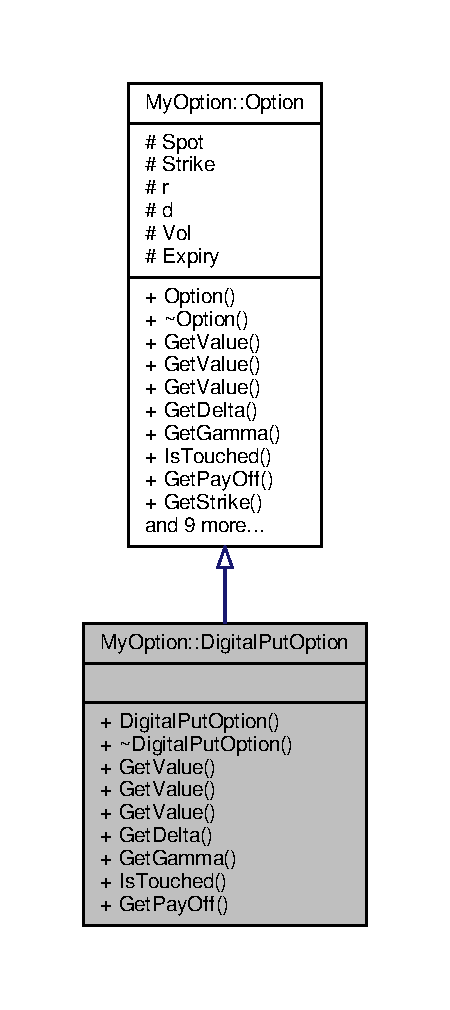
\includegraphics[width=216pt]{classMyOption_1_1DigitalPutOption__inherit__graph}
\end{center}
\end{figure}


Collaboration diagram for My\+Option\+:\+:Digital\+Put\+Option\+:
\nopagebreak
\begin{figure}[H]
\begin{center}
\leavevmode
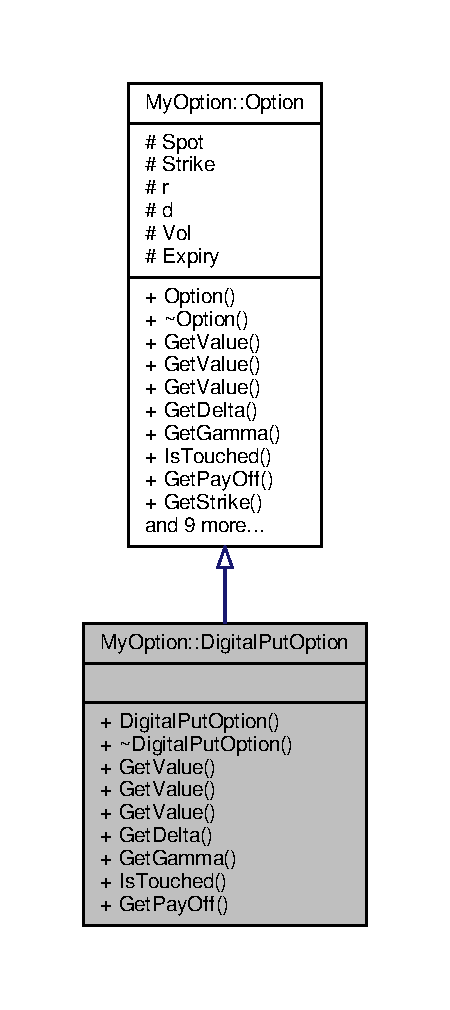
\includegraphics[width=216pt]{classMyOption_1_1DigitalPutOption__coll__graph}
\end{center}
\end{figure}
\subsection*{Public Member Functions}
\begin{DoxyCompactItemize}
\item 
\hyperlink{classMyOption_1_1DigitalPutOption_a06d1c6c093b1bf2a1fcc24e46be8f06f}{Digital\+Put\+Option} (double \hyperlink{classMyOption_1_1Option_a6c6f01d75cde7e92d16a6d8d6f331a1d}{Spot}, double \hyperlink{classMyOption_1_1Option_a3033c483588ce26b175280c7f9dee8d1}{Strike}, double \hyperlink{classMyOption_1_1Option_aa8cb250427dece65ea49255d4102cc8d}{r}, double \hyperlink{classMyOption_1_1Option_a500979f4b32262594d895c4a83b58d1d}{d}, double \hyperlink{classMyOption_1_1Option_a5d6002c14b335c782873bf1437113513}{Vol}, double \hyperlink{classMyOption_1_1Option_ac1adacb417fede41d151b9cda05bcb3d}{Expiry})
\item 
virtual \hyperlink{classMyOption_1_1DigitalPutOption_af373736d79c052e94761072593e37648}{$\sim$\+Digital\+Put\+Option} ()
\item 
virtual double \hyperlink{classMyOption_1_1DigitalPutOption_a4f51d8bdbdddfbebf428cea500c5edf0}{Get\+Value} (double \hyperlink{classMyOption_1_1Option_a6c6f01d75cde7e92d16a6d8d6f331a1d}{Spot})
\item 
virtual double \hyperlink{classMyOption_1_1DigitalPutOption_a3d26c1e53753a199a35f0769672e94cf}{Get\+Value} (double \hyperlink{classMyOption_1_1Option_a6c6f01d75cde7e92d16a6d8d6f331a1d}{Spot}, double \hyperlink{classMyOption_1_1Option_a5d6002c14b335c782873bf1437113513}{Vol}, double \hyperlink{classMyOption_1_1Option_ac1adacb417fede41d151b9cda05bcb3d}{Expiry})
\item 
virtual double \hyperlink{classMyOption_1_1DigitalPutOption_ab55e215fef7a85bb06175a05548a3f77}{Get\+Value} (double \hyperlink{classMyOption_1_1Option_a6c6f01d75cde7e92d16a6d8d6f331a1d}{Spot}, double \hyperlink{classMyOption_1_1Option_aa8cb250427dece65ea49255d4102cc8d}{r}, double \hyperlink{classMyOption_1_1Option_a5d6002c14b335c782873bf1437113513}{Vol}, double \hyperlink{classMyOption_1_1Option_ac1adacb417fede41d151b9cda05bcb3d}{Expiry})
\item 
virtual double \hyperlink{classMyOption_1_1DigitalPutOption_a20e33b1b8a221ea2200fd08f3c691c4a}{Get\+Delta} (double \hyperlink{classMyOption_1_1Option_a6c6f01d75cde7e92d16a6d8d6f331a1d}{Spot}, double \hyperlink{classMyOption_1_1Option_a5d6002c14b335c782873bf1437113513}{Vol}, double \hyperlink{classMyOption_1_1Option_ac1adacb417fede41d151b9cda05bcb3d}{Expiry})
\item 
virtual double \hyperlink{classMyOption_1_1DigitalPutOption_a4eeb4d0c53f0075ee80e67270f4bd6a5}{Get\+Gamma} (double \hyperlink{classMyOption_1_1Option_a6c6f01d75cde7e92d16a6d8d6f331a1d}{Spot}, double \hyperlink{classMyOption_1_1Option_a5d6002c14b335c782873bf1437113513}{Vol}, double \hyperlink{classMyOption_1_1Option_ac1adacb417fede41d151b9cda05bcb3d}{Expiry})
\item 
virtual long \hyperlink{classMyOption_1_1DigitalPutOption_a6e38fdd2a8d6f6f959e5cdb0a66e4057}{Is\+Touched} (double \hyperlink{classMyOption_1_1Option_a6c6f01d75cde7e92d16a6d8d6f331a1d}{Spot}) const
\item 
virtual double \hyperlink{classMyOption_1_1DigitalPutOption_abadcbb78c02b4e6ee22d45da1c72f7b1}{Get\+Pay\+Off} (double \hyperlink{classMyOption_1_1Option_a6c6f01d75cde7e92d16a6d8d6f331a1d}{Spot}) const
\end{DoxyCompactItemize}
\subsection*{Additional Inherited Members}


\subsection{Constructor \& Destructor Documentation}
\hypertarget{classMyOption_1_1DigitalPutOption_a06d1c6c093b1bf2a1fcc24e46be8f06f}{}\label{classMyOption_1_1DigitalPutOption_a06d1c6c093b1bf2a1fcc24e46be8f06f} 
\index{My\+Option\+::\+Digital\+Put\+Option@{My\+Option\+::\+Digital\+Put\+Option}!Digital\+Put\+Option@{Digital\+Put\+Option}}
\index{Digital\+Put\+Option@{Digital\+Put\+Option}!My\+Option\+::\+Digital\+Put\+Option@{My\+Option\+::\+Digital\+Put\+Option}}
\subsubsection{\texorpdfstring{Digital\+Put\+Option()}{DigitalPutOption()}}
{\footnotesize\ttfamily My\+Option\+::\+Digital\+Put\+Option\+::\+Digital\+Put\+Option (\begin{DoxyParamCaption}\item[{double}]{Spot,  }\item[{double}]{Strike,  }\item[{double}]{r,  }\item[{double}]{d,  }\item[{double}]{Vol,  }\item[{double}]{Expiry }\end{DoxyParamCaption})}

\hypertarget{classMyOption_1_1DigitalPutOption_af373736d79c052e94761072593e37648}{}\label{classMyOption_1_1DigitalPutOption_af373736d79c052e94761072593e37648} 
\index{My\+Option\+::\+Digital\+Put\+Option@{My\+Option\+::\+Digital\+Put\+Option}!````~Digital\+Put\+Option@{$\sim$\+Digital\+Put\+Option}}
\index{````~Digital\+Put\+Option@{$\sim$\+Digital\+Put\+Option}!My\+Option\+::\+Digital\+Put\+Option@{My\+Option\+::\+Digital\+Put\+Option}}
\subsubsection{\texorpdfstring{$\sim$\+Digital\+Put\+Option()}{~DigitalPutOption()}}
{\footnotesize\ttfamily virtual My\+Option\+::\+Digital\+Put\+Option\+::$\sim$\+Digital\+Put\+Option (\begin{DoxyParamCaption}{ }\end{DoxyParamCaption})\hspace{0.3cm}{\ttfamily [inline]}, {\ttfamily [virtual]}}



\subsection{Member Function Documentation}
\hypertarget{classMyOption_1_1DigitalPutOption_a20e33b1b8a221ea2200fd08f3c691c4a}{}\label{classMyOption_1_1DigitalPutOption_a20e33b1b8a221ea2200fd08f3c691c4a} 
\index{My\+Option\+::\+Digital\+Put\+Option@{My\+Option\+::\+Digital\+Put\+Option}!Get\+Delta@{Get\+Delta}}
\index{Get\+Delta@{Get\+Delta}!My\+Option\+::\+Digital\+Put\+Option@{My\+Option\+::\+Digital\+Put\+Option}}
\subsubsection{\texorpdfstring{Get\+Delta()}{GetDelta()}}
{\footnotesize\ttfamily virtual double My\+Option\+::\+Digital\+Put\+Option\+::\+Get\+Delta (\begin{DoxyParamCaption}\item[{double}]{Spot,  }\item[{double}]{Vol,  }\item[{double}]{Expiry }\end{DoxyParamCaption})\hspace{0.3cm}{\ttfamily [virtual]}}



Implements \hyperlink{classMyOption_1_1Option_a4947bde99bb5e46b79aa0f36fd353d9b}{My\+Option\+::\+Option}.

\hypertarget{classMyOption_1_1DigitalPutOption_a4eeb4d0c53f0075ee80e67270f4bd6a5}{}\label{classMyOption_1_1DigitalPutOption_a4eeb4d0c53f0075ee80e67270f4bd6a5} 
\index{My\+Option\+::\+Digital\+Put\+Option@{My\+Option\+::\+Digital\+Put\+Option}!Get\+Gamma@{Get\+Gamma}}
\index{Get\+Gamma@{Get\+Gamma}!My\+Option\+::\+Digital\+Put\+Option@{My\+Option\+::\+Digital\+Put\+Option}}
\subsubsection{\texorpdfstring{Get\+Gamma()}{GetGamma()}}
{\footnotesize\ttfamily virtual double My\+Option\+::\+Digital\+Put\+Option\+::\+Get\+Gamma (\begin{DoxyParamCaption}\item[{double}]{Spot,  }\item[{double}]{Vol,  }\item[{double}]{Expiry }\end{DoxyParamCaption})\hspace{0.3cm}{\ttfamily [virtual]}}



Implements \hyperlink{classMyOption_1_1Option_a4416faa432b5004e449394056c7f1363}{My\+Option\+::\+Option}.

\hypertarget{classMyOption_1_1DigitalPutOption_abadcbb78c02b4e6ee22d45da1c72f7b1}{}\label{classMyOption_1_1DigitalPutOption_abadcbb78c02b4e6ee22d45da1c72f7b1} 
\index{My\+Option\+::\+Digital\+Put\+Option@{My\+Option\+::\+Digital\+Put\+Option}!Get\+Pay\+Off@{Get\+Pay\+Off}}
\index{Get\+Pay\+Off@{Get\+Pay\+Off}!My\+Option\+::\+Digital\+Put\+Option@{My\+Option\+::\+Digital\+Put\+Option}}
\subsubsection{\texorpdfstring{Get\+Pay\+Off()}{GetPayOff()}}
{\footnotesize\ttfamily virtual double My\+Option\+::\+Digital\+Put\+Option\+::\+Get\+Pay\+Off (\begin{DoxyParamCaption}\item[{double}]{Spot }\end{DoxyParamCaption}) const\hspace{0.3cm}{\ttfamily [virtual]}}



Implements \hyperlink{classMyOption_1_1Option_a4b6b84dc485153ffadfb32afa9bb52f3}{My\+Option\+::\+Option}.

\hypertarget{classMyOption_1_1DigitalPutOption_a4f51d8bdbdddfbebf428cea500c5edf0}{}\label{classMyOption_1_1DigitalPutOption_a4f51d8bdbdddfbebf428cea500c5edf0} 
\index{My\+Option\+::\+Digital\+Put\+Option@{My\+Option\+::\+Digital\+Put\+Option}!Get\+Value@{Get\+Value}}
\index{Get\+Value@{Get\+Value}!My\+Option\+::\+Digital\+Put\+Option@{My\+Option\+::\+Digital\+Put\+Option}}
\subsubsection{\texorpdfstring{Get\+Value()}{GetValue()}\hspace{0.1cm}{\footnotesize\ttfamily [1/3]}}
{\footnotesize\ttfamily virtual double My\+Option\+::\+Digital\+Put\+Option\+::\+Get\+Value (\begin{DoxyParamCaption}\item[{double}]{Spot }\end{DoxyParamCaption})\hspace{0.3cm}{\ttfamily [virtual]}}



Implements \hyperlink{classMyOption_1_1Option_aff32b402a5e44fca9e5a22a142fbbdd6}{My\+Option\+::\+Option}.

\hypertarget{classMyOption_1_1DigitalPutOption_a3d26c1e53753a199a35f0769672e94cf}{}\label{classMyOption_1_1DigitalPutOption_a3d26c1e53753a199a35f0769672e94cf} 
\index{My\+Option\+::\+Digital\+Put\+Option@{My\+Option\+::\+Digital\+Put\+Option}!Get\+Value@{Get\+Value}}
\index{Get\+Value@{Get\+Value}!My\+Option\+::\+Digital\+Put\+Option@{My\+Option\+::\+Digital\+Put\+Option}}
\subsubsection{\texorpdfstring{Get\+Value()}{GetValue()}\hspace{0.1cm}{\footnotesize\ttfamily [2/3]}}
{\footnotesize\ttfamily virtual double My\+Option\+::\+Digital\+Put\+Option\+::\+Get\+Value (\begin{DoxyParamCaption}\item[{double}]{Spot,  }\item[{double}]{Vol,  }\item[{double}]{Expiry }\end{DoxyParamCaption})\hspace{0.3cm}{\ttfamily [virtual]}}



Implements \hyperlink{classMyOption_1_1Option_a78fa248dcb939e0ebaefbb944d5d9cf8}{My\+Option\+::\+Option}.

\hypertarget{classMyOption_1_1DigitalPutOption_ab55e215fef7a85bb06175a05548a3f77}{}\label{classMyOption_1_1DigitalPutOption_ab55e215fef7a85bb06175a05548a3f77} 
\index{My\+Option\+::\+Digital\+Put\+Option@{My\+Option\+::\+Digital\+Put\+Option}!Get\+Value@{Get\+Value}}
\index{Get\+Value@{Get\+Value}!My\+Option\+::\+Digital\+Put\+Option@{My\+Option\+::\+Digital\+Put\+Option}}
\subsubsection{\texorpdfstring{Get\+Value()}{GetValue()}\hspace{0.1cm}{\footnotesize\ttfamily [3/3]}}
{\footnotesize\ttfamily virtual double My\+Option\+::\+Digital\+Put\+Option\+::\+Get\+Value (\begin{DoxyParamCaption}\item[{double}]{Spot,  }\item[{double}]{r,  }\item[{double}]{Vol,  }\item[{double}]{Expiry }\end{DoxyParamCaption})\hspace{0.3cm}{\ttfamily [virtual]}}



Implements \hyperlink{classMyOption_1_1Option_a62422d3dc60eabe65cfa94d2a452f5f8}{My\+Option\+::\+Option}.

\hypertarget{classMyOption_1_1DigitalPutOption_a6e38fdd2a8d6f6f959e5cdb0a66e4057}{}\label{classMyOption_1_1DigitalPutOption_a6e38fdd2a8d6f6f959e5cdb0a66e4057} 
\index{My\+Option\+::\+Digital\+Put\+Option@{My\+Option\+::\+Digital\+Put\+Option}!Is\+Touched@{Is\+Touched}}
\index{Is\+Touched@{Is\+Touched}!My\+Option\+::\+Digital\+Put\+Option@{My\+Option\+::\+Digital\+Put\+Option}}
\subsubsection{\texorpdfstring{Is\+Touched()}{IsTouched()}}
{\footnotesize\ttfamily virtual long My\+Option\+::\+Digital\+Put\+Option\+::\+Is\+Touched (\begin{DoxyParamCaption}\item[{double}]{Spot }\end{DoxyParamCaption}) const\hspace{0.3cm}{\ttfamily [virtual]}}



Implements \hyperlink{classMyOption_1_1Option_ade57d2fcb9f22f3c2a57d75f55444c33}{My\+Option\+::\+Option}.



The documentation for this class was generated from the following file\+:\begin{DoxyCompactItemize}
\item 
\hyperlink{options_8h}{options.\+h}\end{DoxyCompactItemize}

\hypertarget{classDownAndOutCall}{}\section{Down\+And\+Out\+Call Class Reference}
\label{classDownAndOutCall}\index{Down\+And\+Out\+Call@{Down\+And\+Out\+Call}}


{\ttfamily \#include $<$Options\+To\+Replicate.\+h$>$}



Inheritance diagram for Down\+And\+Out\+Call\+:
\nopagebreak
\begin{figure}[H]
\begin{center}
\leavevmode
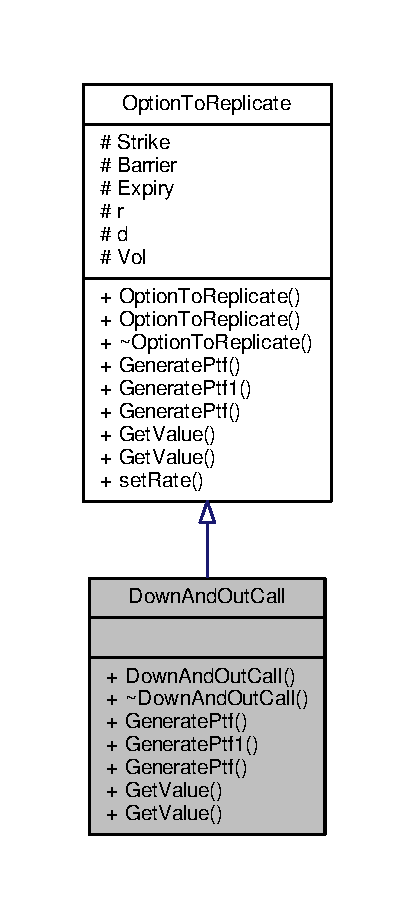
\includegraphics[width=199pt]{classDownAndOutCall__inherit__graph}
\end{center}
\end{figure}


Collaboration diagram for Down\+And\+Out\+Call\+:
\nopagebreak
\begin{figure}[H]
\begin{center}
\leavevmode
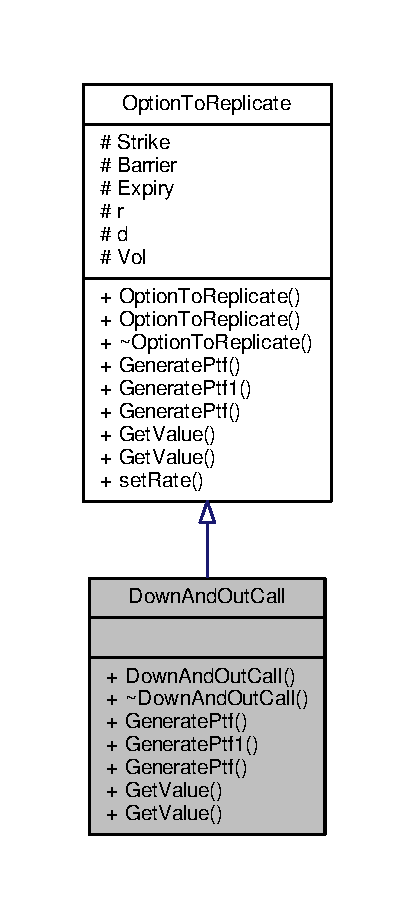
\includegraphics[width=199pt]{classDownAndOutCall__coll__graph}
\end{center}
\end{figure}
\subsection*{Public Member Functions}
\begin{DoxyCompactItemize}
\item 
\hyperlink{classDownAndOutCall_a61cebb82065fba33c51db0a3075a40d8}{Down\+And\+Out\+Call} (double \hyperlink{classOptionToReplicate_a64ffcbc25fc60c5dc18ca4b78194ca89}{Strike}, double \hyperlink{classOptionToReplicate_a7cd35379de855ad6e53008fbf7e9dda0}{Barrier}, double \hyperlink{classOptionToReplicate_ad344ef3a4a4e93372c390c60420d1a61}{r}, double \hyperlink{classOptionToReplicate_a3a28b1ab0cd1ee635b3c31998bd2c572}{Vol}, double \hyperlink{classOptionToReplicate_a62014eac88a2a766ed674be69e9fd926}{Expiry}, double \hyperlink{classOptionToReplicate_aa088a512c974dc622ca1bbca61ec5e34}{d}=0.\+0)
\item 
virtual \hyperlink{classDownAndOutCall_a01a5a9897ef41a37c569187b6c263afb}{$\sim$\+Down\+And\+Out\+Call} ()
\item 
virtual void \hyperlink{classDownAndOutCall_a378b557d728ed157db9d41ef39bb8abf}{Generate\+Ptf} (unsigned long steps, shared\+\_\+ptr$<$ Option $>$ Option\+Final)
\item 
virtual void \hyperlink{classDownAndOutCall_a0b8b44b58822b7c4f75e2436b9cf69d7}{Generate\+Ptf1} (unsigned long steps, shared\+\_\+ptr$<$ Option $>$ Option\+Final)
\item 
virtual void \hyperlink{classDownAndOutCall_a7f4f73437c1e61cc57f96fadd05a7df1}{Generate\+Ptf} (unsigned long steps, const vector$<$ double $>$ \&\hyperlink{classOptionToReplicate_a3a28b1ab0cd1ee635b3c31998bd2c572}{Vol}, shared\+\_\+ptr$<$ Option $>$ Option\+Final)
\item 
virtual double \hyperlink{classDownAndOutCall_ab5855704cc4680238596427a115cb3e1}{Get\+Value} (double \+\_\+\+Spot, double \+\_\+t, shared\+\_\+ptr$<$ Option $>$ Option\+Final) const
\item 
virtual double \hyperlink{classDownAndOutCall_a6ccfc2e5d77a48558087d4b9df914377}{Get\+Value} (double \+\_\+\+Spot, const vector$<$ double $>$ \&\+\_\+\+Vol, double \+\_\+t, shared\+\_\+ptr$<$ Option $>$ Option\+Final) const
\end{DoxyCompactItemize}
\subsection*{Additional Inherited Members}


\subsection{Constructor \& Destructor Documentation}
\hypertarget{classDownAndOutCall_a61cebb82065fba33c51db0a3075a40d8}{}\label{classDownAndOutCall_a61cebb82065fba33c51db0a3075a40d8} 
\index{Down\+And\+Out\+Call@{Down\+And\+Out\+Call}!Down\+And\+Out\+Call@{Down\+And\+Out\+Call}}
\index{Down\+And\+Out\+Call@{Down\+And\+Out\+Call}!Down\+And\+Out\+Call@{Down\+And\+Out\+Call}}
\subsubsection{\texorpdfstring{Down\+And\+Out\+Call()}{DownAndOutCall()}}
{\footnotesize\ttfamily Down\+And\+Out\+Call\+::\+Down\+And\+Out\+Call (\begin{DoxyParamCaption}\item[{double}]{Strike,  }\item[{double}]{Barrier,  }\item[{double}]{r,  }\item[{double}]{Vol,  }\item[{double}]{Expiry,  }\item[{double}]{d = {\ttfamily 0.0} }\end{DoxyParamCaption})}

\hypertarget{classDownAndOutCall_a01a5a9897ef41a37c569187b6c263afb}{}\label{classDownAndOutCall_a01a5a9897ef41a37c569187b6c263afb} 
\index{Down\+And\+Out\+Call@{Down\+And\+Out\+Call}!````~Down\+And\+Out\+Call@{$\sim$\+Down\+And\+Out\+Call}}
\index{````~Down\+And\+Out\+Call@{$\sim$\+Down\+And\+Out\+Call}!Down\+And\+Out\+Call@{Down\+And\+Out\+Call}}
\subsubsection{\texorpdfstring{$\sim$\+Down\+And\+Out\+Call()}{~DownAndOutCall()}}
{\footnotesize\ttfamily virtual Down\+And\+Out\+Call\+::$\sim$\+Down\+And\+Out\+Call (\begin{DoxyParamCaption}{ }\end{DoxyParamCaption})\hspace{0.3cm}{\ttfamily [inline]}, {\ttfamily [virtual]}}



\subsection{Member Function Documentation}
\hypertarget{classDownAndOutCall_a378b557d728ed157db9d41ef39bb8abf}{}\label{classDownAndOutCall_a378b557d728ed157db9d41ef39bb8abf} 
\index{Down\+And\+Out\+Call@{Down\+And\+Out\+Call}!Generate\+Ptf@{Generate\+Ptf}}
\index{Generate\+Ptf@{Generate\+Ptf}!Down\+And\+Out\+Call@{Down\+And\+Out\+Call}}
\subsubsection{\texorpdfstring{Generate\+Ptf()}{GeneratePtf()}\hspace{0.1cm}{\footnotesize\ttfamily [1/2]}}
{\footnotesize\ttfamily virtual void Down\+And\+Out\+Call\+::\+Generate\+Ptf (\begin{DoxyParamCaption}\item[{unsigned long}]{steps,  }\item[{shared\+\_\+ptr$<$ Option $>$}]{Option\+Final }\end{DoxyParamCaption})\hspace{0.3cm}{\ttfamily [virtual]}}



Implements \hyperlink{classOptionToReplicate_ae744ce948286546566cd424eaa7ea5cb}{Option\+To\+Replicate}.

\hypertarget{classDownAndOutCall_a7f4f73437c1e61cc57f96fadd05a7df1}{}\label{classDownAndOutCall_a7f4f73437c1e61cc57f96fadd05a7df1} 
\index{Down\+And\+Out\+Call@{Down\+And\+Out\+Call}!Generate\+Ptf@{Generate\+Ptf}}
\index{Generate\+Ptf@{Generate\+Ptf}!Down\+And\+Out\+Call@{Down\+And\+Out\+Call}}
\subsubsection{\texorpdfstring{Generate\+Ptf()}{GeneratePtf()}\hspace{0.1cm}{\footnotesize\ttfamily [2/2]}}
{\footnotesize\ttfamily virtual void Down\+And\+Out\+Call\+::\+Generate\+Ptf (\begin{DoxyParamCaption}\item[{unsigned long}]{steps,  }\item[{const vector$<$ double $>$ \&}]{Vol,  }\item[{shared\+\_\+ptr$<$ Option $>$}]{Option\+Final }\end{DoxyParamCaption})\hspace{0.3cm}{\ttfamily [virtual]}}



Implements \hyperlink{classOptionToReplicate_a47ad183412648a70cd77957383eb421f}{Option\+To\+Replicate}.

\hypertarget{classDownAndOutCall_a0b8b44b58822b7c4f75e2436b9cf69d7}{}\label{classDownAndOutCall_a0b8b44b58822b7c4f75e2436b9cf69d7} 
\index{Down\+And\+Out\+Call@{Down\+And\+Out\+Call}!Generate\+Ptf1@{Generate\+Ptf1}}
\index{Generate\+Ptf1@{Generate\+Ptf1}!Down\+And\+Out\+Call@{Down\+And\+Out\+Call}}
\subsubsection{\texorpdfstring{Generate\+Ptf1()}{GeneratePtf1()}}
{\footnotesize\ttfamily virtual void Down\+And\+Out\+Call\+::\+Generate\+Ptf1 (\begin{DoxyParamCaption}\item[{unsigned long}]{steps,  }\item[{shared\+\_\+ptr$<$ Option $>$}]{Option\+Final }\end{DoxyParamCaption})\hspace{0.3cm}{\ttfamily [virtual]}}



Implements \hyperlink{classOptionToReplicate_ad3315e5766faa9be46fa690d8d358b9d}{Option\+To\+Replicate}.

\hypertarget{classDownAndOutCall_ab5855704cc4680238596427a115cb3e1}{}\label{classDownAndOutCall_ab5855704cc4680238596427a115cb3e1} 
\index{Down\+And\+Out\+Call@{Down\+And\+Out\+Call}!Get\+Value@{Get\+Value}}
\index{Get\+Value@{Get\+Value}!Down\+And\+Out\+Call@{Down\+And\+Out\+Call}}
\subsubsection{\texorpdfstring{Get\+Value()}{GetValue()}\hspace{0.1cm}{\footnotesize\ttfamily [1/2]}}
{\footnotesize\ttfamily virtual double Down\+And\+Out\+Call\+::\+Get\+Value (\begin{DoxyParamCaption}\item[{double}]{\+\_\+\+Spot,  }\item[{double}]{\+\_\+t,  }\item[{shared\+\_\+ptr$<$ Option $>$}]{Option\+Final }\end{DoxyParamCaption}) const\hspace{0.3cm}{\ttfamily [virtual]}}



Implements \hyperlink{classOptionToReplicate_a7f39f64594b4baffb45d61a65b38c6b2}{Option\+To\+Replicate}.

\hypertarget{classDownAndOutCall_a6ccfc2e5d77a48558087d4b9df914377}{}\label{classDownAndOutCall_a6ccfc2e5d77a48558087d4b9df914377} 
\index{Down\+And\+Out\+Call@{Down\+And\+Out\+Call}!Get\+Value@{Get\+Value}}
\index{Get\+Value@{Get\+Value}!Down\+And\+Out\+Call@{Down\+And\+Out\+Call}}
\subsubsection{\texorpdfstring{Get\+Value()}{GetValue()}\hspace{0.1cm}{\footnotesize\ttfamily [2/2]}}
{\footnotesize\ttfamily virtual double Down\+And\+Out\+Call\+::\+Get\+Value (\begin{DoxyParamCaption}\item[{double}]{\+\_\+\+Spot,  }\item[{const vector$<$ double $>$ \&}]{\+\_\+\+Vol,  }\item[{double}]{\+\_\+t,  }\item[{shared\+\_\+ptr$<$ Option $>$}]{Option\+Final }\end{DoxyParamCaption}) const\hspace{0.3cm}{\ttfamily [virtual]}}



Implements \hyperlink{classOptionToReplicate_a738f813473de4945df377bcd3fe17f6e}{Option\+To\+Replicate}.



The documentation for this class was generated from the following file\+:\begin{DoxyCompactItemize}
\item 
\hyperlink{OptionsToReplicate_8h}{Options\+To\+Replicate.\+h}\end{DoxyCompactItemize}

\hypertarget{classengine__mc__exotic}{}\section{engine\+\_\+mc\+\_\+exotic$<$ T, U $>$ Class Template Reference}
\label{classengine__mc__exotic}\index{engine\+\_\+mc\+\_\+exotic$<$ T, U $>$@{engine\+\_\+mc\+\_\+exotic$<$ T, U $>$}}


{\ttfamily \#include $<$engine\+\_\+exotic.\+h$>$}



Collaboration diagram for engine\+\_\+mc\+\_\+exotic$<$ T, U $>$\+:
\nopagebreak
\begin{figure}[H]
\begin{center}
\leavevmode
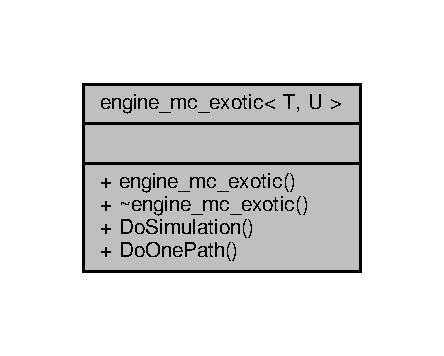
\includegraphics[width=213pt]{classengine__mc__exotic__coll__graph}
\end{center}
\end{figure}
\subsection*{Public Member Functions}
\begin{DoxyCompactItemize}
\item 
\hyperlink{classengine__mc__exotic_ac84b055a4f57a3e08d5a0a0093167b53}{engine\+\_\+mc\+\_\+exotic} (shared\+\_\+ptr$<$ T $>$ \&The\+Option\+\_\+, const \hyperlink{classParameters}{Parameters} \&r\+\_\+, shared\+\_\+ptr$<$ U $>$ \&The\+Paths\+\_\+)
\item 
virtual \hyperlink{classengine__mc__exotic_ab36a687185223f73a36bfe2f1ba6f75d}{$\sim$engine\+\_\+mc\+\_\+exotic} ()
\item 
void \hyperlink{classengine__mc__exotic_a2987115b991c16b43f63dc9f6310ab66}{Do\+Simulation} (\hyperlink{classStatisticsMC}{Statistics\+MC} \&The\+Gatherer, unsigned long Number\+Of\+Paths)
\item 
double \hyperlink{classengine__mc__exotic_a39ee74fd980343bba205ddd7ba482455}{Do\+One\+Path} (const \hyperlink{classMJArray}{M\+J\+Array} \&Spot\+Values) const
\end{DoxyCompactItemize}


\subsection{Constructor \& Destructor Documentation}
\hypertarget{classengine__mc__exotic_ac84b055a4f57a3e08d5a0a0093167b53}{}\label{classengine__mc__exotic_ac84b055a4f57a3e08d5a0a0093167b53} 
\index{engine\+\_\+mc\+\_\+exotic@{engine\+\_\+mc\+\_\+exotic}!engine\+\_\+mc\+\_\+exotic@{engine\+\_\+mc\+\_\+exotic}}
\index{engine\+\_\+mc\+\_\+exotic@{engine\+\_\+mc\+\_\+exotic}!engine\+\_\+mc\+\_\+exotic@{engine\+\_\+mc\+\_\+exotic}}
\subsubsection{\texorpdfstring{engine\+\_\+mc\+\_\+exotic()}{engine\_mc\_exotic()}}
{\footnotesize\ttfamily template$<$typename T , typename U $>$ \\
\hyperlink{classengine__mc__exotic}{engine\+\_\+mc\+\_\+exotic}$<$ T, U $>$\+::\hyperlink{classengine__mc__exotic}{engine\+\_\+mc\+\_\+exotic} (\begin{DoxyParamCaption}\item[{shared\+\_\+ptr$<$ T $>$ \&}]{The\+Option\+\_\+,  }\item[{const \hyperlink{classParameters}{Parameters} \&}]{r\+\_\+,  }\item[{shared\+\_\+ptr$<$ U $>$ \&}]{The\+Paths\+\_\+ }\end{DoxyParamCaption})\hspace{0.3cm}{\ttfamily [inline]}}

\hypertarget{classengine__mc__exotic_ab36a687185223f73a36bfe2f1ba6f75d}{}\label{classengine__mc__exotic_ab36a687185223f73a36bfe2f1ba6f75d} 
\index{engine\+\_\+mc\+\_\+exotic@{engine\+\_\+mc\+\_\+exotic}!````~engine\+\_\+mc\+\_\+exotic@{$\sim$engine\+\_\+mc\+\_\+exotic}}
\index{````~engine\+\_\+mc\+\_\+exotic@{$\sim$engine\+\_\+mc\+\_\+exotic}!engine\+\_\+mc\+\_\+exotic@{engine\+\_\+mc\+\_\+exotic}}
\subsubsection{\texorpdfstring{$\sim$engine\+\_\+mc\+\_\+exotic()}{~engine\_mc\_exotic()}}
{\footnotesize\ttfamily template$<$typename T , typename U $>$ \\
virtual \hyperlink{classengine__mc__exotic}{engine\+\_\+mc\+\_\+exotic}$<$ T, U $>$\+::$\sim$\hyperlink{classengine__mc__exotic}{engine\+\_\+mc\+\_\+exotic} (\begin{DoxyParamCaption}{ }\end{DoxyParamCaption})\hspace{0.3cm}{\ttfamily [inline]}, {\ttfamily [virtual]}}



\subsection{Member Function Documentation}
\hypertarget{classengine__mc__exotic_a39ee74fd980343bba205ddd7ba482455}{}\label{classengine__mc__exotic_a39ee74fd980343bba205ddd7ba482455} 
\index{engine\+\_\+mc\+\_\+exotic@{engine\+\_\+mc\+\_\+exotic}!Do\+One\+Path@{Do\+One\+Path}}
\index{Do\+One\+Path@{Do\+One\+Path}!engine\+\_\+mc\+\_\+exotic@{engine\+\_\+mc\+\_\+exotic}}
\subsubsection{\texorpdfstring{Do\+One\+Path()}{DoOnePath()}}
{\footnotesize\ttfamily template$<$typename T , typename U $>$ \\
double \hyperlink{classengine__mc__exotic}{engine\+\_\+mc\+\_\+exotic}$<$ T, U $>$\+::Do\+One\+Path (\begin{DoxyParamCaption}\item[{const \hyperlink{classMJArray}{M\+J\+Array} \&}]{Spot\+Values }\end{DoxyParamCaption}) const\hspace{0.3cm}{\ttfamily [inline]}}

\hypertarget{classengine__mc__exotic_a2987115b991c16b43f63dc9f6310ab66}{}\label{classengine__mc__exotic_a2987115b991c16b43f63dc9f6310ab66} 
\index{engine\+\_\+mc\+\_\+exotic@{engine\+\_\+mc\+\_\+exotic}!Do\+Simulation@{Do\+Simulation}}
\index{Do\+Simulation@{Do\+Simulation}!engine\+\_\+mc\+\_\+exotic@{engine\+\_\+mc\+\_\+exotic}}
\subsubsection{\texorpdfstring{Do\+Simulation()}{DoSimulation()}}
{\footnotesize\ttfamily template$<$typename T , typename U $>$ \\
void \hyperlink{classengine__mc__exotic}{engine\+\_\+mc\+\_\+exotic}$<$ T, U $>$\+::Do\+Simulation (\begin{DoxyParamCaption}\item[{\hyperlink{classStatisticsMC}{Statistics\+MC} \&}]{The\+Gatherer,  }\item[{unsigned long}]{Number\+Of\+Paths }\end{DoxyParamCaption})\hspace{0.3cm}{\ttfamily [inline]}}



The documentation for this class was generated from the following file\+:\begin{DoxyCompactItemize}
\item 
\hyperlink{engine__exotic_8h}{engine\+\_\+exotic.\+h}\end{DoxyCompactItemize}

\hypertarget{classEngineRepli}{}\section{Engine\+Repli$<$ T, U $>$ Class Template Reference}
\label{classEngineRepli}\index{Engine\+Repli$<$ T, U $>$@{Engine\+Repli$<$ T, U $>$}}


{\ttfamily \#include $<$engine\+\_\+replication.\+h$>$}



Collaboration diagram for Engine\+Repli$<$ T, U $>$\+:
\nopagebreak
\begin{figure}[H]
\begin{center}
\leavevmode
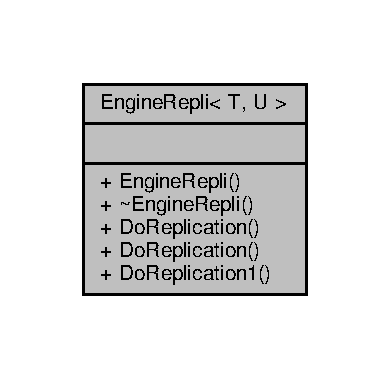
\includegraphics[width=187pt]{classEngineRepli__coll__graph}
\end{center}
\end{figure}
\subsection*{Public Member Functions}
\begin{DoxyCompactItemize}
\item 
\hyperlink{classEngineRepli_a77ada5e83eb12eaf6b19b0826847cb7d}{Engine\+Repli} (shared\+\_\+ptr$<$ T $>$ \&Option\+\_\+, shared\+\_\+ptr$<$ U $>$ \&Final\+Pay\+Off\+\_\+)
\item 
\hyperlink{classEngineRepli_a328a6ae729326cced7a986a94c8fc45e}{$\sim$\+Engine\+Repli} ()
\item 
double \hyperlink{classEngineRepli_a3dcaf8e4c17db01c3293aafd0f38c670}{Do\+Replication} (unsigned long steps, double Spot, double t)
\item 
double \hyperlink{classEngineRepli_ad247f9177127cffcf82bc6603d7ad1db}{Do\+Replication} (unsigned long steps, vector$<$ double $>$ \+\_\+\+Vol, double Spot, double t)
\item 
double \hyperlink{classEngineRepli_a3eac0deeeb53bf5e034b0d643a8191c6}{Do\+Replication1} (unsigned long steps, double Spot, double t)
\end{DoxyCompactItemize}


\subsection{Constructor \& Destructor Documentation}
\hypertarget{classEngineRepli_a77ada5e83eb12eaf6b19b0826847cb7d}{}\label{classEngineRepli_a77ada5e83eb12eaf6b19b0826847cb7d} 
\index{Engine\+Repli@{Engine\+Repli}!Engine\+Repli@{Engine\+Repli}}
\index{Engine\+Repli@{Engine\+Repli}!Engine\+Repli@{Engine\+Repli}}
\subsubsection{\texorpdfstring{Engine\+Repli()}{EngineRepli()}}
{\footnotesize\ttfamily template$<$typename T , typename U $>$ \\
\hyperlink{classEngineRepli}{Engine\+Repli}$<$ T, U $>$\+::\hyperlink{classEngineRepli}{Engine\+Repli} (\begin{DoxyParamCaption}\item[{shared\+\_\+ptr$<$ T $>$ \&}]{Option\+\_\+,  }\item[{shared\+\_\+ptr$<$ U $>$ \&}]{Final\+Pay\+Off\+\_\+ }\end{DoxyParamCaption})\hspace{0.3cm}{\ttfamily [inline]}}

\hypertarget{classEngineRepli_a328a6ae729326cced7a986a94c8fc45e}{}\label{classEngineRepli_a328a6ae729326cced7a986a94c8fc45e} 
\index{Engine\+Repli@{Engine\+Repli}!````~Engine\+Repli@{$\sim$\+Engine\+Repli}}
\index{````~Engine\+Repli@{$\sim$\+Engine\+Repli}!Engine\+Repli@{Engine\+Repli}}
\subsubsection{\texorpdfstring{$\sim$\+Engine\+Repli()}{~EngineRepli()}}
{\footnotesize\ttfamily template$<$typename T , typename U $>$ \\
\hyperlink{classEngineRepli}{Engine\+Repli}$<$ T, U $>$\+::$\sim$\hyperlink{classEngineRepli}{Engine\+Repli} (\begin{DoxyParamCaption}{ }\end{DoxyParamCaption})\hspace{0.3cm}{\ttfamily [inline]}}



\subsection{Member Function Documentation}
\hypertarget{classEngineRepli_a3dcaf8e4c17db01c3293aafd0f38c670}{}\label{classEngineRepli_a3dcaf8e4c17db01c3293aafd0f38c670} 
\index{Engine\+Repli@{Engine\+Repli}!Do\+Replication@{Do\+Replication}}
\index{Do\+Replication@{Do\+Replication}!Engine\+Repli@{Engine\+Repli}}
\subsubsection{\texorpdfstring{Do\+Replication()}{DoReplication()}\hspace{0.1cm}{\footnotesize\ttfamily [1/2]}}
{\footnotesize\ttfamily template$<$typename T , typename U $>$ \\
double \hyperlink{classEngineRepli}{Engine\+Repli}$<$ T, U $>$\+::Do\+Replication (\begin{DoxyParamCaption}\item[{unsigned long}]{steps,  }\item[{double}]{Spot,  }\item[{double}]{t }\end{DoxyParamCaption})\hspace{0.3cm}{\ttfamily [inline]}}

\hypertarget{classEngineRepli_ad247f9177127cffcf82bc6603d7ad1db}{}\label{classEngineRepli_ad247f9177127cffcf82bc6603d7ad1db} 
\index{Engine\+Repli@{Engine\+Repli}!Do\+Replication@{Do\+Replication}}
\index{Do\+Replication@{Do\+Replication}!Engine\+Repli@{Engine\+Repli}}
\subsubsection{\texorpdfstring{Do\+Replication()}{DoReplication()}\hspace{0.1cm}{\footnotesize\ttfamily [2/2]}}
{\footnotesize\ttfamily template$<$typename T , typename U $>$ \\
double \hyperlink{classEngineRepli}{Engine\+Repli}$<$ T, U $>$\+::Do\+Replication (\begin{DoxyParamCaption}\item[{unsigned long}]{steps,  }\item[{vector$<$ double $>$}]{\+\_\+\+Vol,  }\item[{double}]{Spot,  }\item[{double}]{t }\end{DoxyParamCaption})\hspace{0.3cm}{\ttfamily [inline]}}

\hypertarget{classEngineRepli_a3eac0deeeb53bf5e034b0d643a8191c6}{}\label{classEngineRepli_a3eac0deeeb53bf5e034b0d643a8191c6} 
\index{Engine\+Repli@{Engine\+Repli}!Do\+Replication1@{Do\+Replication1}}
\index{Do\+Replication1@{Do\+Replication1}!Engine\+Repli@{Engine\+Repli}}
\subsubsection{\texorpdfstring{Do\+Replication1()}{DoReplication1()}}
{\footnotesize\ttfamily template$<$typename T , typename U $>$ \\
double \hyperlink{classEngineRepli}{Engine\+Repli}$<$ T, U $>$\+::Do\+Replication1 (\begin{DoxyParamCaption}\item[{unsigned long}]{steps,  }\item[{double}]{Spot,  }\item[{double}]{t }\end{DoxyParamCaption})\hspace{0.3cm}{\ttfamily [inline]}}



The documentation for this class was generated from the following file\+:\begin{DoxyCompactItemize}
\item 
\hyperlink{engine__replication_8h}{engine\+\_\+replication.\+h}\end{DoxyCompactItemize}

\hypertarget{classEngineSimul}{}\section{Engine\+Simul$<$ T $>$ Class Template Reference}
\label{classEngineSimul}\index{Engine\+Simul$<$ T $>$@{Engine\+Simul$<$ T $>$}}


{\ttfamily \#include $<$engine\+\_\+simul.\+h$>$}



Collaboration diagram for Engine\+Simul$<$ T $>$\+:
\nopagebreak
\begin{figure}[H]
\begin{center}
\leavevmode
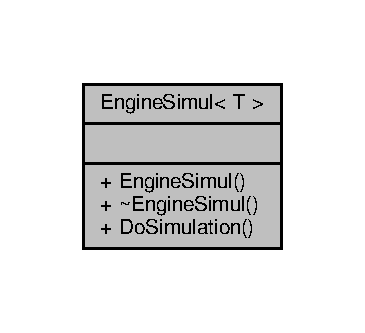
\includegraphics[width=175pt]{classEngineSimul__coll__graph}
\end{center}
\end{figure}
\subsection*{Public Member Functions}
\begin{DoxyCompactItemize}
\item 
\hyperlink{classEngineSimul_a3d3243c9166e293532db8ad623657177}{Engine\+Simul} (shared\+\_\+ptr$<$ \hyperlink{classHedgingStrategy}{Hedging\+Strategy}$<$ T $>$$>$ The\+Hedging\+Strategy\+\_\+, unsigned long Number\+Of\+Paths\+\_\+)
\item 
\hyperlink{classEngineSimul_a82c248f5bd2d2b65348e0fec22c2a0e1}{$\sim$\+Engine\+Simul} ()
\item 
double \hyperlink{classEngineSimul_a7a7733a90fcc7e20bf4e0a3b9eb03d6d}{Do\+Simulation} () const
\end{DoxyCompactItemize}


\subsection{Constructor \& Destructor Documentation}
\hypertarget{classEngineSimul_a3d3243c9166e293532db8ad623657177}{}\label{classEngineSimul_a3d3243c9166e293532db8ad623657177} 
\index{Engine\+Simul@{Engine\+Simul}!Engine\+Simul@{Engine\+Simul}}
\index{Engine\+Simul@{Engine\+Simul}!Engine\+Simul@{Engine\+Simul}}
\subsubsection{\texorpdfstring{Engine\+Simul()}{EngineSimul()}}
{\footnotesize\ttfamily template$<$typename T $>$ \\
\hyperlink{classEngineSimul}{Engine\+Simul}$<$ T $>$\+::\hyperlink{classEngineSimul}{Engine\+Simul} (\begin{DoxyParamCaption}\item[{shared\+\_\+ptr$<$ \hyperlink{classHedgingStrategy}{Hedging\+Strategy}$<$ T $>$$>$}]{The\+Hedging\+Strategy\+\_\+,  }\item[{unsigned long}]{Number\+Of\+Paths\+\_\+ }\end{DoxyParamCaption})}

\hypertarget{classEngineSimul_a82c248f5bd2d2b65348e0fec22c2a0e1}{}\label{classEngineSimul_a82c248f5bd2d2b65348e0fec22c2a0e1} 
\index{Engine\+Simul@{Engine\+Simul}!````~Engine\+Simul@{$\sim$\+Engine\+Simul}}
\index{````~Engine\+Simul@{$\sim$\+Engine\+Simul}!Engine\+Simul@{Engine\+Simul}}
\subsubsection{\texorpdfstring{$\sim$\+Engine\+Simul()}{~EngineSimul()}}
{\footnotesize\ttfamily template$<$typename T $>$ \\
\hyperlink{classEngineSimul}{Engine\+Simul}$<$ T $>$\+::$\sim$\hyperlink{classEngineSimul}{Engine\+Simul} (\begin{DoxyParamCaption}{ }\end{DoxyParamCaption})\hspace{0.3cm}{\ttfamily [inline]}}



\subsection{Member Function Documentation}
\hypertarget{classEngineSimul_a7a7733a90fcc7e20bf4e0a3b9eb03d6d}{}\label{classEngineSimul_a7a7733a90fcc7e20bf4e0a3b9eb03d6d} 
\index{Engine\+Simul@{Engine\+Simul}!Do\+Simulation@{Do\+Simulation}}
\index{Do\+Simulation@{Do\+Simulation}!Engine\+Simul@{Engine\+Simul}}
\subsubsection{\texorpdfstring{Do\+Simulation()}{DoSimulation()}}
{\footnotesize\ttfamily template$<$typename T $>$ \\
double \hyperlink{classEngineSimul}{Engine\+Simul}$<$ T $>$\+::Do\+Simulation (\begin{DoxyParamCaption}{ }\end{DoxyParamCaption}) const}



The documentation for this class was generated from the following file\+:\begin{DoxyCompactItemize}
\item 
\hyperlink{engine__simul_8h}{engine\+\_\+simul.\+h}\end{DoxyCompactItemize}

\hypertarget{classEngineSimulSV}{}\section{Engine\+Simul\+SV$<$ T $>$ Class Template Reference}
\label{classEngineSimulSV}\index{Engine\+Simul\+S\+V$<$ T $>$@{Engine\+Simul\+S\+V$<$ T $>$}}


{\ttfamily \#include $<$engine\+\_\+simul.\+h$>$}



Collaboration diagram for Engine\+Simul\+SV$<$ T $>$\+:
\nopagebreak
\begin{figure}[H]
\begin{center}
\leavevmode
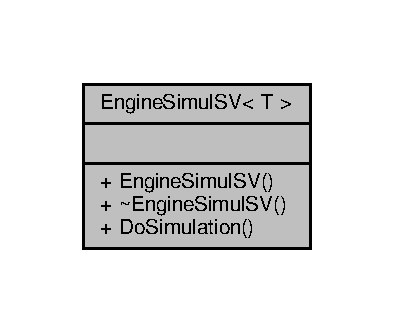
\includegraphics[width=189pt]{classEngineSimulSV__coll__graph}
\end{center}
\end{figure}
\subsection*{Public Member Functions}
\begin{DoxyCompactItemize}
\item 
\hyperlink{classEngineSimulSV_a07498f7d0c424f4e7f79be663933a5f4}{Engine\+Simul\+SV} (shared\+\_\+ptr$<$ \hyperlink{classHedgingStrategySV}{Hedging\+Strategy\+SV}$<$ T $>$$>$ The\+Hedging\+Strategy\+\_\+, unsigned long Number\+Of\+Paths\+\_\+)
\item 
\hyperlink{classEngineSimulSV_a3d2d099c94f7ff0a717cc85769413f72}{$\sim$\+Engine\+Simul\+SV} ()
\item 
double \hyperlink{classEngineSimulSV_a1883c6f71ba18603fc28b03415c8c0dd}{Do\+Simulation} () const
\end{DoxyCompactItemize}


\subsection{Constructor \& Destructor Documentation}
\hypertarget{classEngineSimulSV_a07498f7d0c424f4e7f79be663933a5f4}{}\label{classEngineSimulSV_a07498f7d0c424f4e7f79be663933a5f4} 
\index{Engine\+Simul\+SV@{Engine\+Simul\+SV}!Engine\+Simul\+SV@{Engine\+Simul\+SV}}
\index{Engine\+Simul\+SV@{Engine\+Simul\+SV}!Engine\+Simul\+SV@{Engine\+Simul\+SV}}
\subsubsection{\texorpdfstring{Engine\+Simul\+S\+V()}{EngineSimulSV()}}
{\footnotesize\ttfamily template$<$typename T $>$ \\
\hyperlink{classEngineSimulSV}{Engine\+Simul\+SV}$<$ T $>$\+::\hyperlink{classEngineSimulSV}{Engine\+Simul\+SV} (\begin{DoxyParamCaption}\item[{shared\+\_\+ptr$<$ \hyperlink{classHedgingStrategySV}{Hedging\+Strategy\+SV}$<$ T $>$$>$}]{The\+Hedging\+Strategy\+\_\+,  }\item[{unsigned long}]{Number\+Of\+Paths\+\_\+ }\end{DoxyParamCaption})}

\hypertarget{classEngineSimulSV_a3d2d099c94f7ff0a717cc85769413f72}{}\label{classEngineSimulSV_a3d2d099c94f7ff0a717cc85769413f72} 
\index{Engine\+Simul\+SV@{Engine\+Simul\+SV}!````~Engine\+Simul\+SV@{$\sim$\+Engine\+Simul\+SV}}
\index{````~Engine\+Simul\+SV@{$\sim$\+Engine\+Simul\+SV}!Engine\+Simul\+SV@{Engine\+Simul\+SV}}
\subsubsection{\texorpdfstring{$\sim$\+Engine\+Simul\+S\+V()}{~EngineSimulSV()}}
{\footnotesize\ttfamily template$<$typename T $>$ \\
\hyperlink{classEngineSimulSV}{Engine\+Simul\+SV}$<$ T $>$\+::$\sim$\hyperlink{classEngineSimulSV}{Engine\+Simul\+SV} (\begin{DoxyParamCaption}{ }\end{DoxyParamCaption})\hspace{0.3cm}{\ttfamily [inline]}}



\subsection{Member Function Documentation}
\hypertarget{classEngineSimulSV_a1883c6f71ba18603fc28b03415c8c0dd}{}\label{classEngineSimulSV_a1883c6f71ba18603fc28b03415c8c0dd} 
\index{Engine\+Simul\+SV@{Engine\+Simul\+SV}!Do\+Simulation@{Do\+Simulation}}
\index{Do\+Simulation@{Do\+Simulation}!Engine\+Simul\+SV@{Engine\+Simul\+SV}}
\subsubsection{\texorpdfstring{Do\+Simulation()}{DoSimulation()}}
{\footnotesize\ttfamily template$<$typename T $>$ \\
double \hyperlink{classEngineSimulSV}{Engine\+Simul\+SV}$<$ T $>$\+::Do\+Simulation (\begin{DoxyParamCaption}{ }\end{DoxyParamCaption}) const}



The documentation for this class was generated from the following file\+:\begin{DoxyCompactItemize}
\item 
\hyperlink{engine__simul_8h}{engine\+\_\+simul.\+h}\end{DoxyCompactItemize}

\hypertarget{classExchangeOption}{}\section{Exchange\+Option Class Reference}
\label{classExchangeOption}\index{Exchange\+Option@{Exchange\+Option}}


{\ttfamily \#include $<$Pay\+Off\+Multi.\+h$>$}



Inheritance diagram for Exchange\+Option\+:
\nopagebreak
\begin{figure}[H]
\begin{center}
\leavevmode
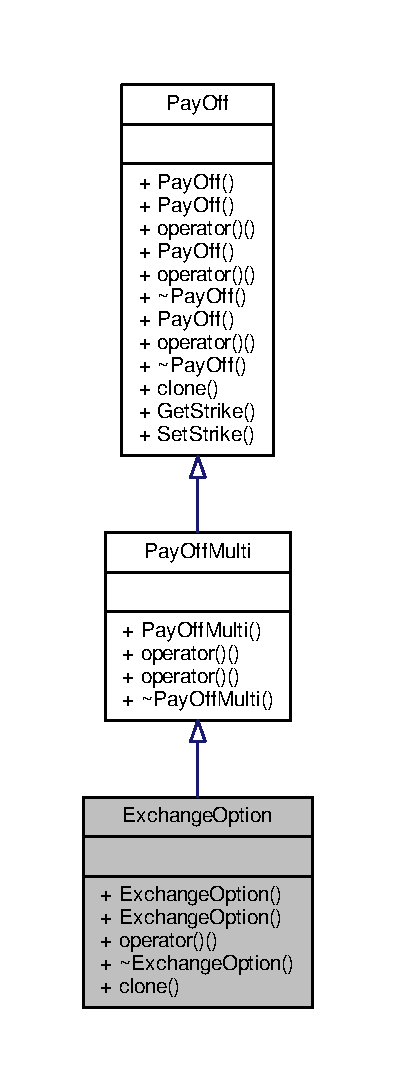
\includegraphics[width=190pt]{classExchangeOption__inherit__graph}
\end{center}
\end{figure}


Collaboration diagram for Exchange\+Option\+:
\nopagebreak
\begin{figure}[H]
\begin{center}
\leavevmode
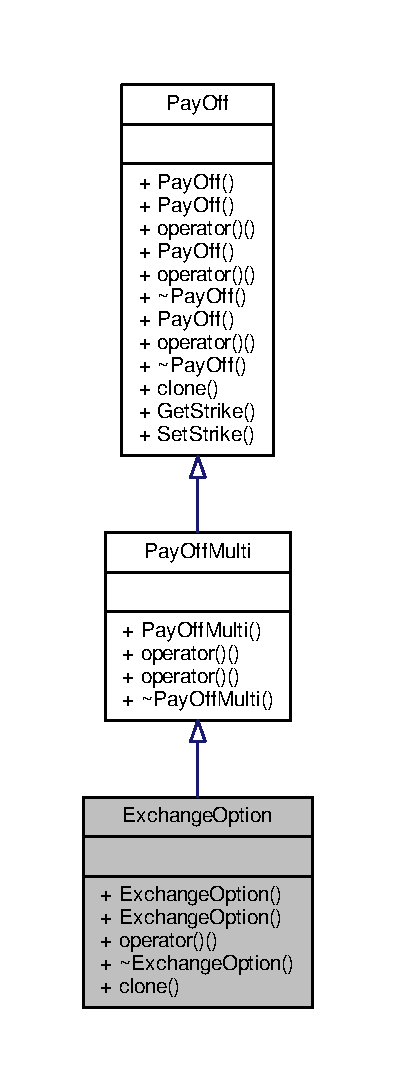
\includegraphics[width=190pt]{classExchangeOption__coll__graph}
\end{center}
\end{figure}
\subsection*{Public Member Functions}
\begin{DoxyCompactItemize}
\item 
\hyperlink{classExchangeOption_a191e8afcc8384e43506d3c13e8dac6c5}{Exchange\+Option} ()
\item 
\hyperlink{classExchangeOption_a642fa4a55bab2deb15a4069824fcd581}{Exchange\+Option} (const \hyperlink{classMJArray}{M\+J\+Array} \&\hyperlink{path__generation_8h_a75c13cde2074f502cc4348c70528572d}{args})
\item 
virtual double \hyperlink{classExchangeOption_ae8d49f6d9d482c1e835e3f1c12a1a905}{operator()} (const \hyperlink{classMJArray}{M\+J\+Array} \&Spots) const
\item 
virtual \hyperlink{classExchangeOption_a4a68daa19012f51f02e3eba95373118c}{$\sim$\+Exchange\+Option} ()
\item 
virtual \hyperlink{classPayOff}{Pay\+Off} $\ast$ \hyperlink{classExchangeOption_ac780838b87eff5b33af728e5e38c1475}{clone} () const
\end{DoxyCompactItemize}
\subsection*{Additional Inherited Members}


\subsection{Constructor \& Destructor Documentation}
\hypertarget{classExchangeOption_a191e8afcc8384e43506d3c13e8dac6c5}{}\label{classExchangeOption_a191e8afcc8384e43506d3c13e8dac6c5} 
\index{Exchange\+Option@{Exchange\+Option}!Exchange\+Option@{Exchange\+Option}}
\index{Exchange\+Option@{Exchange\+Option}!Exchange\+Option@{Exchange\+Option}}
\subsubsection{\texorpdfstring{Exchange\+Option()}{ExchangeOption()}\hspace{0.1cm}{\footnotesize\ttfamily [1/2]}}
{\footnotesize\ttfamily Exchange\+Option\+::\+Exchange\+Option (\begin{DoxyParamCaption}{ }\end{DoxyParamCaption})}

\hypertarget{classExchangeOption_a642fa4a55bab2deb15a4069824fcd581}{}\label{classExchangeOption_a642fa4a55bab2deb15a4069824fcd581} 
\index{Exchange\+Option@{Exchange\+Option}!Exchange\+Option@{Exchange\+Option}}
\index{Exchange\+Option@{Exchange\+Option}!Exchange\+Option@{Exchange\+Option}}
\subsubsection{\texorpdfstring{Exchange\+Option()}{ExchangeOption()}\hspace{0.1cm}{\footnotesize\ttfamily [2/2]}}
{\footnotesize\ttfamily Exchange\+Option\+::\+Exchange\+Option (\begin{DoxyParamCaption}\item[{const \hyperlink{classMJArray}{M\+J\+Array} \&}]{args }\end{DoxyParamCaption})}

\hypertarget{classExchangeOption_a4a68daa19012f51f02e3eba95373118c}{}\label{classExchangeOption_a4a68daa19012f51f02e3eba95373118c} 
\index{Exchange\+Option@{Exchange\+Option}!````~Exchange\+Option@{$\sim$\+Exchange\+Option}}
\index{````~Exchange\+Option@{$\sim$\+Exchange\+Option}!Exchange\+Option@{Exchange\+Option}}
\subsubsection{\texorpdfstring{$\sim$\+Exchange\+Option()}{~ExchangeOption()}}
{\footnotesize\ttfamily virtual Exchange\+Option\+::$\sim$\+Exchange\+Option (\begin{DoxyParamCaption}{ }\end{DoxyParamCaption})\hspace{0.3cm}{\ttfamily [inline]}, {\ttfamily [virtual]}}



\subsection{Member Function Documentation}
\hypertarget{classExchangeOption_ac780838b87eff5b33af728e5e38c1475}{}\label{classExchangeOption_ac780838b87eff5b33af728e5e38c1475} 
\index{Exchange\+Option@{Exchange\+Option}!clone@{clone}}
\index{clone@{clone}!Exchange\+Option@{Exchange\+Option}}
\subsubsection{\texorpdfstring{clone()}{clone()}}
{\footnotesize\ttfamily virtual \hyperlink{classPayOff}{Pay\+Off}$\ast$ Exchange\+Option\+::clone (\begin{DoxyParamCaption}{ }\end{DoxyParamCaption}) const\hspace{0.3cm}{\ttfamily [virtual]}}



Implements \hyperlink{classPayOff_ad8194d5b82247ae89c25c515f0ba806a}{Pay\+Off}.

\hypertarget{classExchangeOption_ae8d49f6d9d482c1e835e3f1c12a1a905}{}\label{classExchangeOption_ae8d49f6d9d482c1e835e3f1c12a1a905} 
\index{Exchange\+Option@{Exchange\+Option}!operator()@{operator()}}
\index{operator()@{operator()}!Exchange\+Option@{Exchange\+Option}}
\subsubsection{\texorpdfstring{operator()()}{operator()()}}
{\footnotesize\ttfamily virtual double Exchange\+Option\+::operator() (\begin{DoxyParamCaption}\item[{const \hyperlink{classMJArray}{M\+J\+Array} \&}]{Spots }\end{DoxyParamCaption}) const\hspace{0.3cm}{\ttfamily [virtual]}}



Implements \hyperlink{classPayOffMulti_a61039e0c0ee136842b5d6f340b9f8155}{Pay\+Off\+Multi}.



The documentation for this class was generated from the following file\+:\begin{DoxyCompactItemize}
\item 
\hyperlink{PayOffMulti_8h}{Pay\+Off\+Multi.\+h}\end{DoxyCompactItemize}

\hypertarget{classExoticBSEngine}{}\section{Exotic\+B\+S\+Engine Class Reference}
\label{classExoticBSEngine}\index{Exotic\+B\+S\+Engine@{Exotic\+B\+S\+Engine}}


{\ttfamily \#include $<$Exotic\+B\+S\+Engine.\+h$>$}



Inheritance diagram for Exotic\+B\+S\+Engine\+:
\nopagebreak
\begin{figure}[H]
\begin{center}
\leavevmode
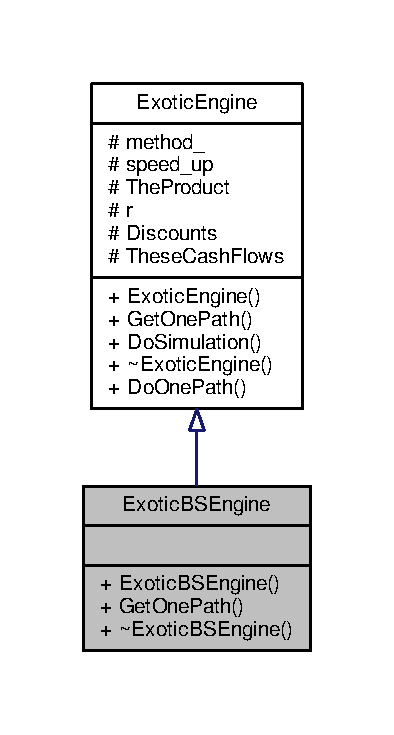
\includegraphics[width=189pt]{classExoticBSEngine__inherit__graph}
\end{center}
\end{figure}


Collaboration diagram for Exotic\+B\+S\+Engine\+:
\nopagebreak
\begin{figure}[H]
\begin{center}
\leavevmode
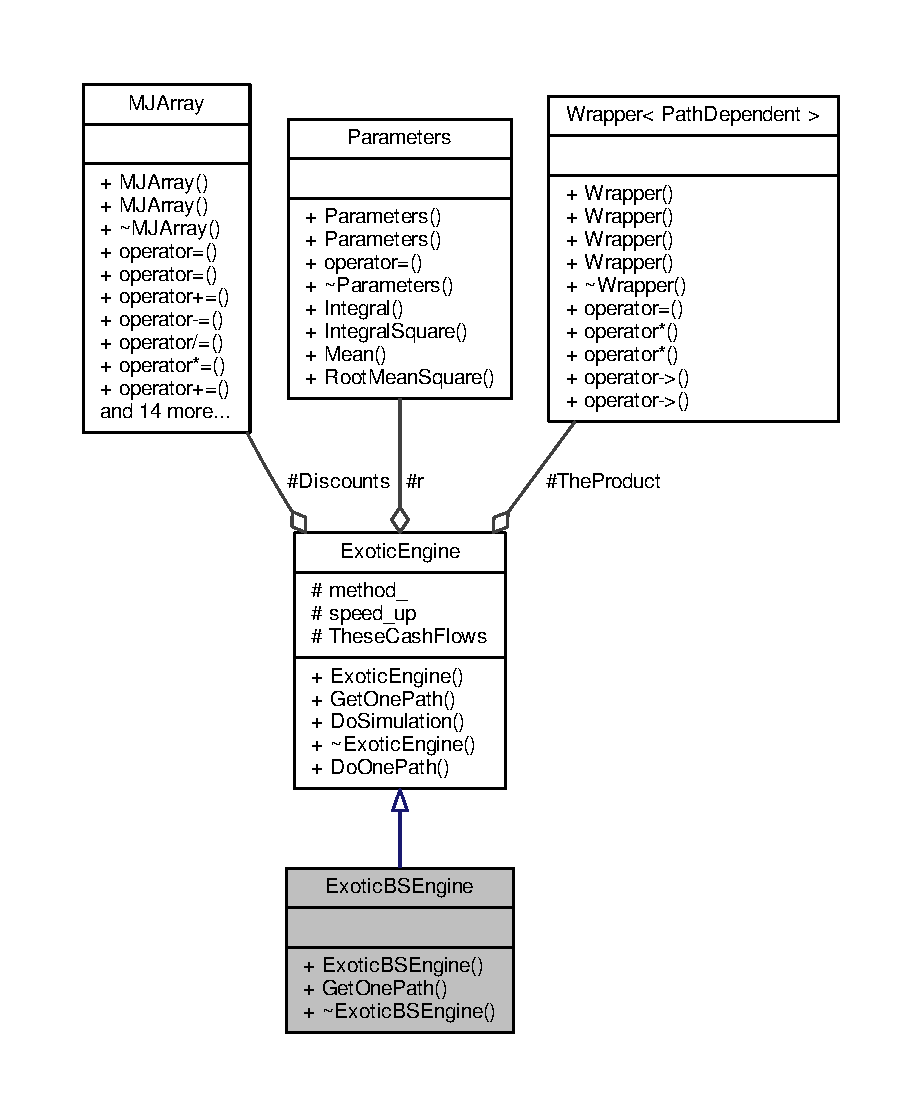
\includegraphics[width=350pt]{classExoticBSEngine__coll__graph}
\end{center}
\end{figure}
\subsection*{Public Member Functions}
\begin{DoxyCompactItemize}
\item 
\hyperlink{classExoticBSEngine_a8a54a128a72a82acfa40e6f144775350}{Exotic\+B\+S\+Engine} (const \hyperlink{classWrapper}{Wrapper}$<$ \hyperlink{classPathDependent}{Path\+Dependent} $>$ \&The\+Product\+\_\+, const \hyperlink{classParameters}{Parameters} \&R\+\_\+, const \hyperlink{classParameters}{Parameters} \&D\+\_\+, const \hyperlink{classParameters}{Parameters} \&Vol\+\_\+, const \hyperlink{classWrapper}{Wrapper}$<$ \hyperlink{classRandomBase}{Random\+Base} $>$ \&The\+Generator\+\_\+, double Spot\+\_\+, bool speed\+\_\+up\+\_\+=false)
\item 
virtual void \hyperlink{classExoticBSEngine_a4f621796857e8cf1b867d66daea2d690}{Get\+One\+Path} (\hyperlink{classMJArray}{M\+J\+Array} \&Log\+Spot\+Values)
\item 
virtual \hyperlink{classExoticBSEngine_a7c957a183892ed4cb5cf5f8969070921}{$\sim$\+Exotic\+B\+S\+Engine} ()
\end{DoxyCompactItemize}
\subsection*{Additional Inherited Members}


\subsection{Constructor \& Destructor Documentation}
\hypertarget{classExoticBSEngine_a8a54a128a72a82acfa40e6f144775350}{}\label{classExoticBSEngine_a8a54a128a72a82acfa40e6f144775350} 
\index{Exotic\+B\+S\+Engine@{Exotic\+B\+S\+Engine}!Exotic\+B\+S\+Engine@{Exotic\+B\+S\+Engine}}
\index{Exotic\+B\+S\+Engine@{Exotic\+B\+S\+Engine}!Exotic\+B\+S\+Engine@{Exotic\+B\+S\+Engine}}
\subsubsection{\texorpdfstring{Exotic\+B\+S\+Engine()}{ExoticBSEngine()}}
{\footnotesize\ttfamily Exotic\+B\+S\+Engine\+::\+Exotic\+B\+S\+Engine (\begin{DoxyParamCaption}\item[{const \hyperlink{classWrapper}{Wrapper}$<$ \hyperlink{classPathDependent}{Path\+Dependent} $>$ \&}]{The\+Product\+\_\+,  }\item[{const \hyperlink{classParameters}{Parameters} \&}]{R\+\_\+,  }\item[{const \hyperlink{classParameters}{Parameters} \&}]{D\+\_\+,  }\item[{const \hyperlink{classParameters}{Parameters} \&}]{Vol\+\_\+,  }\item[{const \hyperlink{classWrapper}{Wrapper}$<$ \hyperlink{classRandomBase}{Random\+Base} $>$ \&}]{The\+Generator\+\_\+,  }\item[{double}]{Spot\+\_\+,  }\item[{bool}]{speed\+\_\+up\+\_\+ = {\ttfamily false} }\end{DoxyParamCaption})}

\hypertarget{classExoticBSEngine_a7c957a183892ed4cb5cf5f8969070921}{}\label{classExoticBSEngine_a7c957a183892ed4cb5cf5f8969070921} 
\index{Exotic\+B\+S\+Engine@{Exotic\+B\+S\+Engine}!````~Exotic\+B\+S\+Engine@{$\sim$\+Exotic\+B\+S\+Engine}}
\index{````~Exotic\+B\+S\+Engine@{$\sim$\+Exotic\+B\+S\+Engine}!Exotic\+B\+S\+Engine@{Exotic\+B\+S\+Engine}}
\subsubsection{\texorpdfstring{$\sim$\+Exotic\+B\+S\+Engine()}{~ExoticBSEngine()}}
{\footnotesize\ttfamily virtual Exotic\+B\+S\+Engine\+::$\sim$\+Exotic\+B\+S\+Engine (\begin{DoxyParamCaption}{ }\end{DoxyParamCaption})\hspace{0.3cm}{\ttfamily [inline]}, {\ttfamily [virtual]}}



\subsection{Member Function Documentation}
\hypertarget{classExoticBSEngine_a4f621796857e8cf1b867d66daea2d690}{}\label{classExoticBSEngine_a4f621796857e8cf1b867d66daea2d690} 
\index{Exotic\+B\+S\+Engine@{Exotic\+B\+S\+Engine}!Get\+One\+Path@{Get\+One\+Path}}
\index{Get\+One\+Path@{Get\+One\+Path}!Exotic\+B\+S\+Engine@{Exotic\+B\+S\+Engine}}
\subsubsection{\texorpdfstring{Get\+One\+Path()}{GetOnePath()}}
{\footnotesize\ttfamily virtual void Exotic\+B\+S\+Engine\+::\+Get\+One\+Path (\begin{DoxyParamCaption}\item[{\hyperlink{classMJArray}{M\+J\+Array} \&}]{Log\+Spot\+Values }\end{DoxyParamCaption})\hspace{0.3cm}{\ttfamily [virtual]}}



Implements \hyperlink{classExoticEngine_a1be567d24e89abadb95bb2af7224b54e}{Exotic\+Engine}.



The documentation for this class was generated from the following file\+:\begin{DoxyCompactItemize}
\item 
\hyperlink{ExoticBSEngine_8h}{Exotic\+B\+S\+Engine.\+h}\end{DoxyCompactItemize}

\hypertarget{classExoticBSEngineBB}{}\section{Exotic\+B\+S\+Engine\+BB Class Reference}
\label{classExoticBSEngineBB}\index{Exotic\+B\+S\+Engine\+BB@{Exotic\+B\+S\+Engine\+BB}}


{\ttfamily \#include $<$Exotic\+B\+S\+Engine\+B\+B.\+h$>$}



Inheritance diagram for Exotic\+B\+S\+Engine\+BB\+:
\nopagebreak
\begin{figure}[H]
\begin{center}
\leavevmode
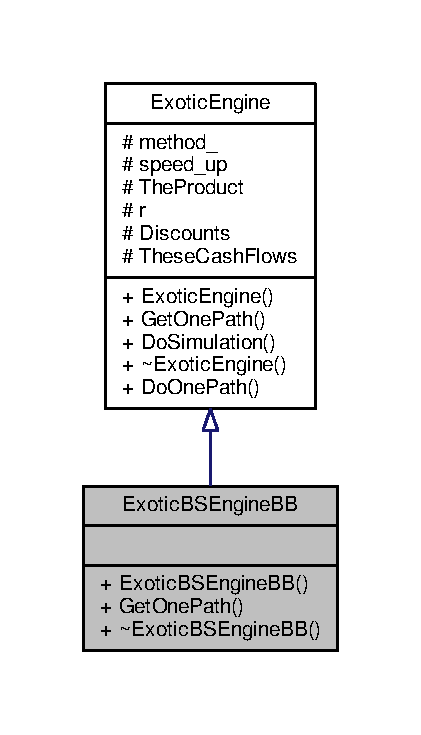
\includegraphics[width=202pt]{classExoticBSEngineBB__inherit__graph}
\end{center}
\end{figure}


Collaboration diagram for Exotic\+B\+S\+Engine\+BB\+:
\nopagebreak
\begin{figure}[H]
\begin{center}
\leavevmode
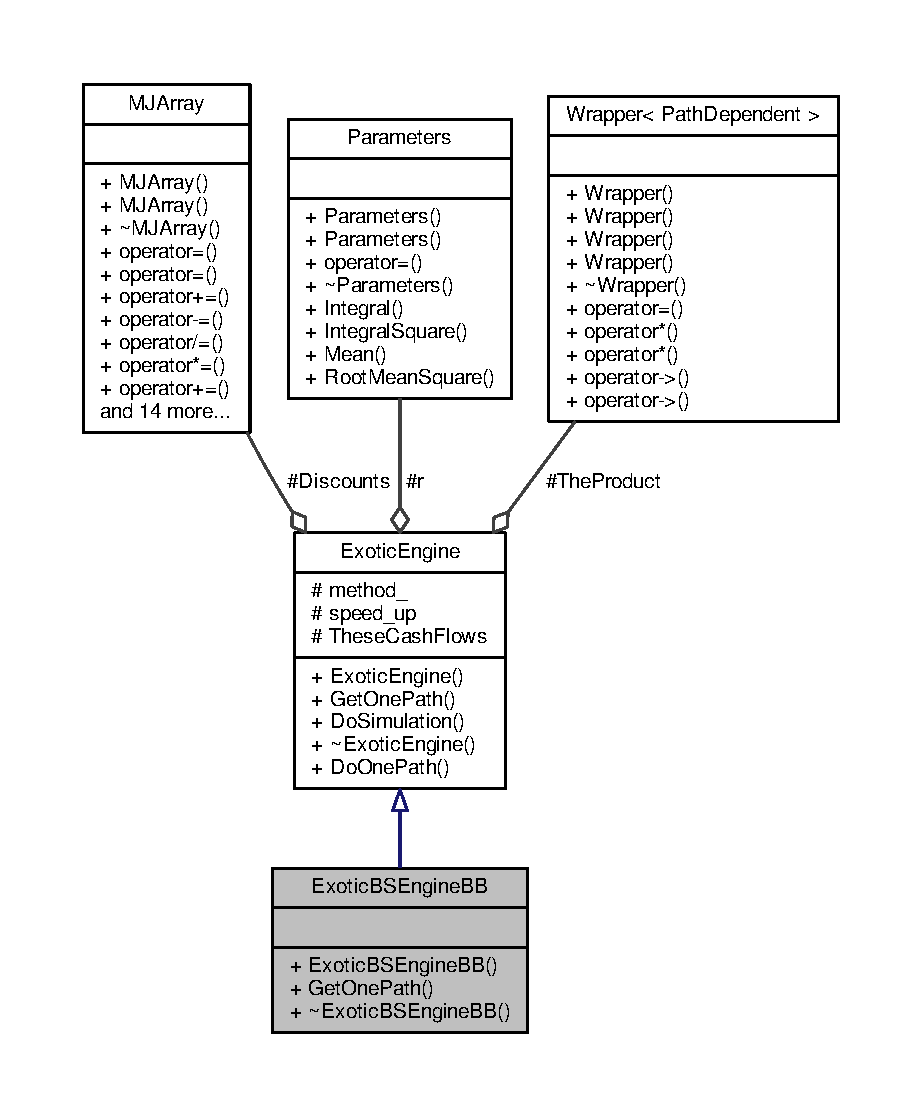
\includegraphics[width=350pt]{classExoticBSEngineBB__coll__graph}
\end{center}
\end{figure}
\subsection*{Public Member Functions}
\begin{DoxyCompactItemize}
\item 
\hyperlink{classExoticBSEngineBB_af8f524ef061a0ff7fda07a90ace2c794}{Exotic\+B\+S\+Engine\+BB} (const \hyperlink{classWrapper}{Wrapper}$<$ \hyperlink{classPathDependent}{Path\+Dependent} $>$ \&The\+Product\+\_\+, const \hyperlink{classParameters}{Parameters} \&R\+\_\+, const \hyperlink{classParameters}{Parameters} \&D\+\_\+, const \hyperlink{classParameters}{Parameters} \&Vol\+\_\+, const \hyperlink{classWrapper}{Wrapper}$<$ \hyperlink{classRandomBase}{Random\+Base} $>$ \&The\+Generator\+\_\+, double Spot\+\_\+, bool speed\+\_\+up\+\_\+=false)
\item 
virtual void \hyperlink{classExoticBSEngineBB_ad11cfbdc7c2096d8493e0de6eb1eec4b}{Get\+One\+Path} (\hyperlink{classMJArray}{M\+J\+Array} \&Log\+Spot\+Values)
\item 
virtual \hyperlink{classExoticBSEngineBB_ab0cec2f243a827428ae1546b42acd57d}{$\sim$\+Exotic\+B\+S\+Engine\+BB} ()
\end{DoxyCompactItemize}
\subsection*{Additional Inherited Members}


\subsection{Constructor \& Destructor Documentation}
\hypertarget{classExoticBSEngineBB_af8f524ef061a0ff7fda07a90ace2c794}{}\label{classExoticBSEngineBB_af8f524ef061a0ff7fda07a90ace2c794} 
\index{Exotic\+B\+S\+Engine\+BB@{Exotic\+B\+S\+Engine\+BB}!Exotic\+B\+S\+Engine\+BB@{Exotic\+B\+S\+Engine\+BB}}
\index{Exotic\+B\+S\+Engine\+BB@{Exotic\+B\+S\+Engine\+BB}!Exotic\+B\+S\+Engine\+BB@{Exotic\+B\+S\+Engine\+BB}}
\subsubsection{\texorpdfstring{Exotic\+B\+S\+Engine\+B\+B()}{ExoticBSEngineBB()}}
{\footnotesize\ttfamily Exotic\+B\+S\+Engine\+B\+B\+::\+Exotic\+B\+S\+Engine\+BB (\begin{DoxyParamCaption}\item[{const \hyperlink{classWrapper}{Wrapper}$<$ \hyperlink{classPathDependent}{Path\+Dependent} $>$ \&}]{The\+Product\+\_\+,  }\item[{const \hyperlink{classParameters}{Parameters} \&}]{R\+\_\+,  }\item[{const \hyperlink{classParameters}{Parameters} \&}]{D\+\_\+,  }\item[{const \hyperlink{classParameters}{Parameters} \&}]{Vol\+\_\+,  }\item[{const \hyperlink{classWrapper}{Wrapper}$<$ \hyperlink{classRandomBase}{Random\+Base} $>$ \&}]{The\+Generator\+\_\+,  }\item[{double}]{Spot\+\_\+,  }\item[{bool}]{speed\+\_\+up\+\_\+ = {\ttfamily false} }\end{DoxyParamCaption})}

\hypertarget{classExoticBSEngineBB_ab0cec2f243a827428ae1546b42acd57d}{}\label{classExoticBSEngineBB_ab0cec2f243a827428ae1546b42acd57d} 
\index{Exotic\+B\+S\+Engine\+BB@{Exotic\+B\+S\+Engine\+BB}!````~Exotic\+B\+S\+Engine\+BB@{$\sim$\+Exotic\+B\+S\+Engine\+BB}}
\index{````~Exotic\+B\+S\+Engine\+BB@{$\sim$\+Exotic\+B\+S\+Engine\+BB}!Exotic\+B\+S\+Engine\+BB@{Exotic\+B\+S\+Engine\+BB}}
\subsubsection{\texorpdfstring{$\sim$\+Exotic\+B\+S\+Engine\+B\+B()}{~ExoticBSEngineBB()}}
{\footnotesize\ttfamily virtual Exotic\+B\+S\+Engine\+B\+B\+::$\sim$\+Exotic\+B\+S\+Engine\+BB (\begin{DoxyParamCaption}{ }\end{DoxyParamCaption})\hspace{0.3cm}{\ttfamily [inline]}, {\ttfamily [virtual]}}



\subsection{Member Function Documentation}
\hypertarget{classExoticBSEngineBB_ad11cfbdc7c2096d8493e0de6eb1eec4b}{}\label{classExoticBSEngineBB_ad11cfbdc7c2096d8493e0de6eb1eec4b} 
\index{Exotic\+B\+S\+Engine\+BB@{Exotic\+B\+S\+Engine\+BB}!Get\+One\+Path@{Get\+One\+Path}}
\index{Get\+One\+Path@{Get\+One\+Path}!Exotic\+B\+S\+Engine\+BB@{Exotic\+B\+S\+Engine\+BB}}
\subsubsection{\texorpdfstring{Get\+One\+Path()}{GetOnePath()}}
{\footnotesize\ttfamily virtual void Exotic\+B\+S\+Engine\+B\+B\+::\+Get\+One\+Path (\begin{DoxyParamCaption}\item[{\hyperlink{classMJArray}{M\+J\+Array} \&}]{Log\+Spot\+Values }\end{DoxyParamCaption})\hspace{0.3cm}{\ttfamily [virtual]}}



Implements \hyperlink{classExoticEngine_a1be567d24e89abadb95bb2af7224b54e}{Exotic\+Engine}.



The documentation for this class was generated from the following file\+:\begin{DoxyCompactItemize}
\item 
\hyperlink{ExoticBSEngineBB_8h}{Exotic\+B\+S\+Engine\+B\+B.\+h}\end{DoxyCompactItemize}

\hypertarget{classExoticBSEnginePCA}{}\section{Exotic\+B\+S\+Engine\+P\+CA Class Reference}
\label{classExoticBSEnginePCA}\index{Exotic\+B\+S\+Engine\+P\+CA@{Exotic\+B\+S\+Engine\+P\+CA}}


{\ttfamily \#include $<$Exotic\+B\+S\+Engine\+P\+C\+A.\+h$>$}



Inheritance diagram for Exotic\+B\+S\+Engine\+P\+CA\+:
\nopagebreak
\begin{figure}[H]
\begin{center}
\leavevmode
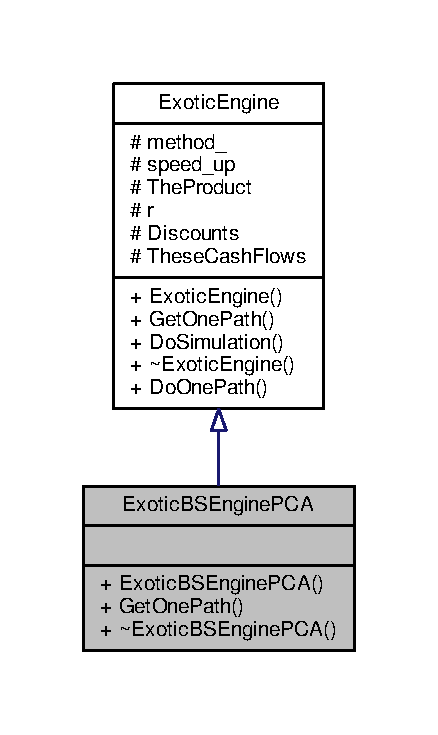
\includegraphics[width=210pt]{classExoticBSEnginePCA__inherit__graph}
\end{center}
\end{figure}


Collaboration diagram for Exotic\+B\+S\+Engine\+P\+CA\+:
\nopagebreak
\begin{figure}[H]
\begin{center}
\leavevmode
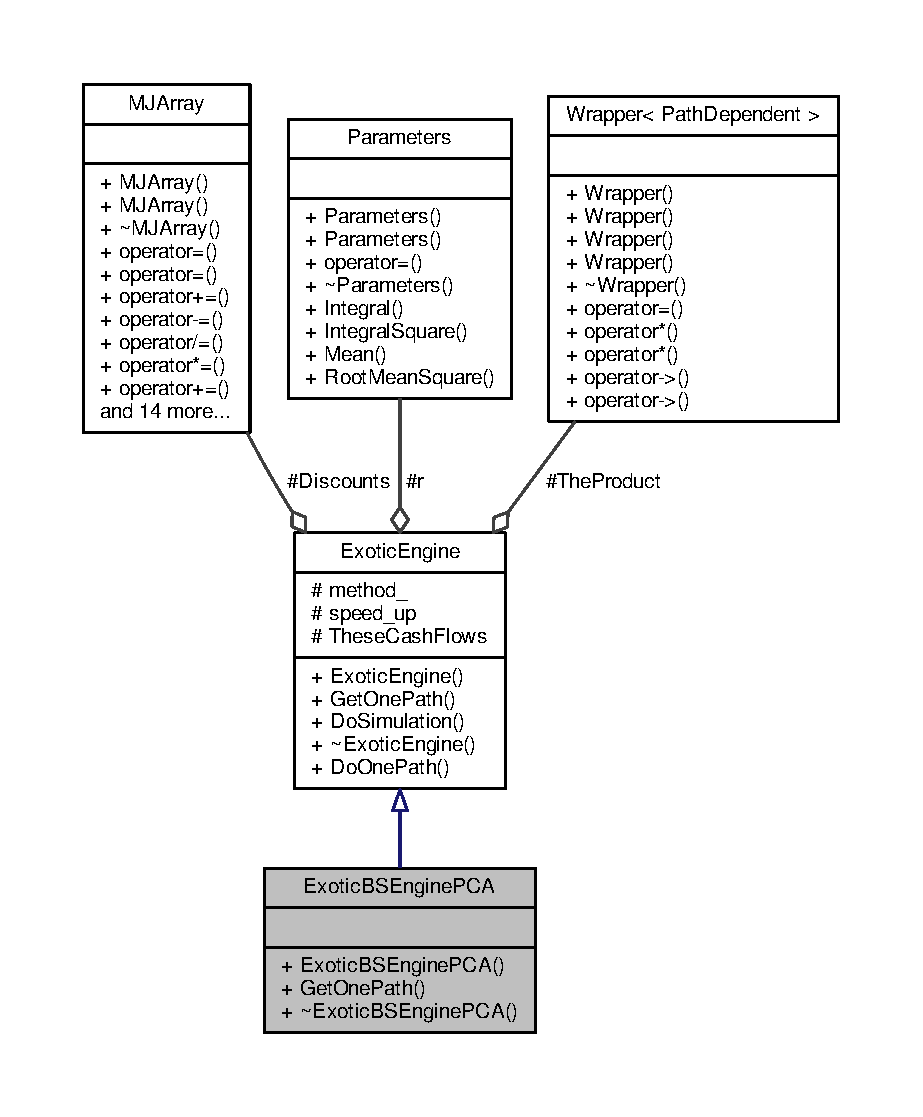
\includegraphics[width=350pt]{classExoticBSEnginePCA__coll__graph}
\end{center}
\end{figure}
\subsection*{Public Member Functions}
\begin{DoxyCompactItemize}
\item 
\hyperlink{classExoticBSEnginePCA_ae91326f64b7a09fdf3d72383cad6dd8f}{Exotic\+B\+S\+Engine\+P\+CA} (const \hyperlink{classWrapper}{Wrapper}$<$ \hyperlink{classPathDependent}{Path\+Dependent} $>$ \&The\+Product\+\_\+, const \hyperlink{classParameters}{Parameters} \&R\+\_\+, const \hyperlink{classParameters}{Parameters} \&D\+\_\+, const \hyperlink{classParameters}{Parameters} \&Vol\+\_\+, const \hyperlink{classWrapper}{Wrapper}$<$ \hyperlink{classRandomBase}{Random\+Base} $>$ \&The\+Generator\+\_\+, double Spot\+\_\+, bool speed\+\_\+up\+\_\+=false)
\item 
virtual void \hyperlink{classExoticBSEnginePCA_ad34270f94895d699ff3d3a0ebc020e9f}{Get\+One\+Path} (\hyperlink{classMJArray}{M\+J\+Array} \&Log\+Spot\+Values)
\item 
virtual \hyperlink{classExoticBSEnginePCA_a6bff4b8aa95aef41294fb707c78d8331}{$\sim$\+Exotic\+B\+S\+Engine\+P\+CA} ()
\end{DoxyCompactItemize}
\subsection*{Additional Inherited Members}


\subsection{Constructor \& Destructor Documentation}
\hypertarget{classExoticBSEnginePCA_ae91326f64b7a09fdf3d72383cad6dd8f}{}\label{classExoticBSEnginePCA_ae91326f64b7a09fdf3d72383cad6dd8f} 
\index{Exotic\+B\+S\+Engine\+P\+CA@{Exotic\+B\+S\+Engine\+P\+CA}!Exotic\+B\+S\+Engine\+P\+CA@{Exotic\+B\+S\+Engine\+P\+CA}}
\index{Exotic\+B\+S\+Engine\+P\+CA@{Exotic\+B\+S\+Engine\+P\+CA}!Exotic\+B\+S\+Engine\+P\+CA@{Exotic\+B\+S\+Engine\+P\+CA}}
\subsubsection{\texorpdfstring{Exotic\+B\+S\+Engine\+P\+C\+A()}{ExoticBSEnginePCA()}}
{\footnotesize\ttfamily Exotic\+B\+S\+Engine\+P\+C\+A\+::\+Exotic\+B\+S\+Engine\+P\+CA (\begin{DoxyParamCaption}\item[{const \hyperlink{classWrapper}{Wrapper}$<$ \hyperlink{classPathDependent}{Path\+Dependent} $>$ \&}]{The\+Product\+\_\+,  }\item[{const \hyperlink{classParameters}{Parameters} \&}]{R\+\_\+,  }\item[{const \hyperlink{classParameters}{Parameters} \&}]{D\+\_\+,  }\item[{const \hyperlink{classParameters}{Parameters} \&}]{Vol\+\_\+,  }\item[{const \hyperlink{classWrapper}{Wrapper}$<$ \hyperlink{classRandomBase}{Random\+Base} $>$ \&}]{The\+Generator\+\_\+,  }\item[{double}]{Spot\+\_\+,  }\item[{bool}]{speed\+\_\+up\+\_\+ = {\ttfamily false} }\end{DoxyParamCaption})}

\hypertarget{classExoticBSEnginePCA_a6bff4b8aa95aef41294fb707c78d8331}{}\label{classExoticBSEnginePCA_a6bff4b8aa95aef41294fb707c78d8331} 
\index{Exotic\+B\+S\+Engine\+P\+CA@{Exotic\+B\+S\+Engine\+P\+CA}!````~Exotic\+B\+S\+Engine\+P\+CA@{$\sim$\+Exotic\+B\+S\+Engine\+P\+CA}}
\index{````~Exotic\+B\+S\+Engine\+P\+CA@{$\sim$\+Exotic\+B\+S\+Engine\+P\+CA}!Exotic\+B\+S\+Engine\+P\+CA@{Exotic\+B\+S\+Engine\+P\+CA}}
\subsubsection{\texorpdfstring{$\sim$\+Exotic\+B\+S\+Engine\+P\+C\+A()}{~ExoticBSEnginePCA()}}
{\footnotesize\ttfamily virtual Exotic\+B\+S\+Engine\+P\+C\+A\+::$\sim$\+Exotic\+B\+S\+Engine\+P\+CA (\begin{DoxyParamCaption}{ }\end{DoxyParamCaption})\hspace{0.3cm}{\ttfamily [inline]}, {\ttfamily [virtual]}}



\subsection{Member Function Documentation}
\hypertarget{classExoticBSEnginePCA_ad34270f94895d699ff3d3a0ebc020e9f}{}\label{classExoticBSEnginePCA_ad34270f94895d699ff3d3a0ebc020e9f} 
\index{Exotic\+B\+S\+Engine\+P\+CA@{Exotic\+B\+S\+Engine\+P\+CA}!Get\+One\+Path@{Get\+One\+Path}}
\index{Get\+One\+Path@{Get\+One\+Path}!Exotic\+B\+S\+Engine\+P\+CA@{Exotic\+B\+S\+Engine\+P\+CA}}
\subsubsection{\texorpdfstring{Get\+One\+Path()}{GetOnePath()}}
{\footnotesize\ttfamily virtual void Exotic\+B\+S\+Engine\+P\+C\+A\+::\+Get\+One\+Path (\begin{DoxyParamCaption}\item[{\hyperlink{classMJArray}{M\+J\+Array} \&}]{Log\+Spot\+Values }\end{DoxyParamCaption})\hspace{0.3cm}{\ttfamily [virtual]}}



Implements \hyperlink{classExoticEngine_a1be567d24e89abadb95bb2af7224b54e}{Exotic\+Engine}.



The documentation for this class was generated from the following file\+:\begin{DoxyCompactItemize}
\item 
\hyperlink{ExoticBSEnginePCA_8h}{Exotic\+B\+S\+Engine\+P\+C\+A.\+h}\end{DoxyCompactItemize}

\hypertarget{classExoticBSEngineReverse}{}\section{Exotic\+B\+S\+Engine\+Reverse Class Reference}
\label{classExoticBSEngineReverse}\index{Exotic\+B\+S\+Engine\+Reverse@{Exotic\+B\+S\+Engine\+Reverse}}


{\ttfamily \#include $<$Exotic\+B\+S\+Engine\+Reverse.\+h$>$}



Inheritance diagram for Exotic\+B\+S\+Engine\+Reverse\+:
\nopagebreak
\begin{figure}[H]
\begin{center}
\leavevmode
\includegraphics[width=226pt]{classExoticBSEngineReverse__inherit__graph}
\end{center}
\end{figure}


Collaboration diagram for Exotic\+B\+S\+Engine\+Reverse\+:
\nopagebreak
\begin{figure}[H]
\begin{center}
\leavevmode
\includegraphics[width=350pt]{classExoticBSEngineReverse__coll__graph}
\end{center}
\end{figure}
\subsection*{Public Member Functions}
\begin{DoxyCompactItemize}
\item 
\hyperlink{classExoticBSEngineReverse_ad8068252390378408d6baa71d4c0049a}{Exotic\+B\+S\+Engine\+Reverse} (const \hyperlink{classWrapper}{Wrapper}$<$ \hyperlink{classPathDependent}{Path\+Dependent} $>$ \&The\+Product\+\_\+, const \hyperlink{classParameters}{Parameters} \&R\+\_\+, const \hyperlink{classParameters}{Parameters} \&D\+\_\+, const \hyperlink{classParameters}{Parameters} \&Vol\+\_\+, const \hyperlink{classWrapper}{Wrapper}$<$ \hyperlink{classRandomBase}{Random\+Base} $>$ \&The\+Generator\+\_\+, double Spot\+\_\+, bool speed\+\_\+up\+\_\+=false)
\item 
virtual void \hyperlink{classExoticBSEngineReverse_ad60a172cfb94070d61b07c4140949b74}{Get\+One\+Path} (\hyperlink{classMJArray}{M\+J\+Array} \&Log\+Spot\+Values)
\item 
virtual \hyperlink{classExoticBSEngineReverse_af436a230e87f2b0fc2b4508010e8eb49}{$\sim$\+Exotic\+B\+S\+Engine\+Reverse} ()
\end{DoxyCompactItemize}
\subsection*{Additional Inherited Members}


\subsection{Constructor \& Destructor Documentation}
\hypertarget{classExoticBSEngineReverse_ad8068252390378408d6baa71d4c0049a}{}\label{classExoticBSEngineReverse_ad8068252390378408d6baa71d4c0049a} 
\index{Exotic\+B\+S\+Engine\+Reverse@{Exotic\+B\+S\+Engine\+Reverse}!Exotic\+B\+S\+Engine\+Reverse@{Exotic\+B\+S\+Engine\+Reverse}}
\index{Exotic\+B\+S\+Engine\+Reverse@{Exotic\+B\+S\+Engine\+Reverse}!Exotic\+B\+S\+Engine\+Reverse@{Exotic\+B\+S\+Engine\+Reverse}}
\subsubsection{\texorpdfstring{Exotic\+B\+S\+Engine\+Reverse()}{ExoticBSEngineReverse()}}
{\footnotesize\ttfamily Exotic\+B\+S\+Engine\+Reverse\+::\+Exotic\+B\+S\+Engine\+Reverse (\begin{DoxyParamCaption}\item[{const \hyperlink{classWrapper}{Wrapper}$<$ \hyperlink{classPathDependent}{Path\+Dependent} $>$ \&}]{The\+Product\+\_\+,  }\item[{const \hyperlink{classParameters}{Parameters} \&}]{R\+\_\+,  }\item[{const \hyperlink{classParameters}{Parameters} \&}]{D\+\_\+,  }\item[{const \hyperlink{classParameters}{Parameters} \&}]{Vol\+\_\+,  }\item[{const \hyperlink{classWrapper}{Wrapper}$<$ \hyperlink{classRandomBase}{Random\+Base} $>$ \&}]{The\+Generator\+\_\+,  }\item[{double}]{Spot\+\_\+,  }\item[{bool}]{speed\+\_\+up\+\_\+ = {\ttfamily false} }\end{DoxyParamCaption})}

\hypertarget{classExoticBSEngineReverse_af436a230e87f2b0fc2b4508010e8eb49}{}\label{classExoticBSEngineReverse_af436a230e87f2b0fc2b4508010e8eb49} 
\index{Exotic\+B\+S\+Engine\+Reverse@{Exotic\+B\+S\+Engine\+Reverse}!````~Exotic\+B\+S\+Engine\+Reverse@{$\sim$\+Exotic\+B\+S\+Engine\+Reverse}}
\index{````~Exotic\+B\+S\+Engine\+Reverse@{$\sim$\+Exotic\+B\+S\+Engine\+Reverse}!Exotic\+B\+S\+Engine\+Reverse@{Exotic\+B\+S\+Engine\+Reverse}}
\subsubsection{\texorpdfstring{$\sim$\+Exotic\+B\+S\+Engine\+Reverse()}{~ExoticBSEngineReverse()}}
{\footnotesize\ttfamily virtual Exotic\+B\+S\+Engine\+Reverse\+::$\sim$\+Exotic\+B\+S\+Engine\+Reverse (\begin{DoxyParamCaption}{ }\end{DoxyParamCaption})\hspace{0.3cm}{\ttfamily [inline]}, {\ttfamily [virtual]}}



\subsection{Member Function Documentation}
\hypertarget{classExoticBSEngineReverse_ad60a172cfb94070d61b07c4140949b74}{}\label{classExoticBSEngineReverse_ad60a172cfb94070d61b07c4140949b74} 
\index{Exotic\+B\+S\+Engine\+Reverse@{Exotic\+B\+S\+Engine\+Reverse}!Get\+One\+Path@{Get\+One\+Path}}
\index{Get\+One\+Path@{Get\+One\+Path}!Exotic\+B\+S\+Engine\+Reverse@{Exotic\+B\+S\+Engine\+Reverse}}
\subsubsection{\texorpdfstring{Get\+One\+Path()}{GetOnePath()}}
{\footnotesize\ttfamily virtual void Exotic\+B\+S\+Engine\+Reverse\+::\+Get\+One\+Path (\begin{DoxyParamCaption}\item[{\hyperlink{classMJArray}{M\+J\+Array} \&}]{Log\+Spot\+Values }\end{DoxyParamCaption})\hspace{0.3cm}{\ttfamily [virtual]}}



Implements \hyperlink{classExoticEngine_a1be567d24e89abadb95bb2af7224b54e}{Exotic\+Engine}.



The documentation for this class was generated from the following file\+:\begin{DoxyCompactItemize}
\item 
\hyperlink{ExoticBSEngineReverse_8h}{Exotic\+B\+S\+Engine\+Reverse.\+h}\end{DoxyCompactItemize}

\hypertarget{classExoticEngine}{}\section{Exotic\+Engine Class Reference}
\label{classExoticEngine}\index{Exotic\+Engine@{Exotic\+Engine}}


{\ttfamily \#include $<$Exotic\+Engine.\+h$>$}



Inheritance diagram for Exotic\+Engine\+:
\nopagebreak
\begin{figure}[H]
\begin{center}
\leavevmode
\includegraphics[width=350pt]{classExoticEngine__inherit__graph}
\end{center}
\end{figure}


Collaboration diagram for Exotic\+Engine\+:
\nopagebreak
\begin{figure}[H]
\begin{center}
\leavevmode
\includegraphics[width=350pt]{classExoticEngine__coll__graph}
\end{center}
\end{figure}
\subsection*{Public Member Functions}
\begin{DoxyCompactItemize}
\item 
\hyperlink{classExoticEngine_a8f2b07aae083e53933b539a9e36df536}{Exotic\+Engine} (const \hyperlink{classWrapper}{Wrapper}$<$ \hyperlink{classPathDependent}{Path\+Dependent} $>$ \&The\+Product\+\_\+, const \hyperlink{classParameters}{Parameters} \&r\+\_\+, bool speed\+\_\+up\+\_\+=false)
\item 
virtual void \hyperlink{classExoticEngine_a1be567d24e89abadb95bb2af7224b54e}{Get\+One\+Path} (\hyperlink{classMJArray}{M\+J\+Array} \&Log\+Spot\+Values)=0
\item 
void \hyperlink{classExoticEngine_a50efae4a77089d6a596153c9c94f1412}{Do\+Simulation} (\hyperlink{classStatisticsMC}{Statistics\+MC} \&The\+Gatherer, unsigned long Number\+Of\+Paths)
\item 
virtual \hyperlink{classExoticEngine_a9ca6c7fadc943a9f00460ae6371bd6a2}{$\sim$\+Exotic\+Engine} ()
\item 
double \hyperlink{classExoticEngine_ac52ddfbb69f3bd1aa2f87114406e1725}{Do\+One\+Path} (const \hyperlink{classMJArray}{M\+J\+Array} \&Spot\+Values) const
\end{DoxyCompactItemize}
\subsection*{Protected Attributes}
\begin{DoxyCompactItemize}
\item 
\hyperlink{PathDependent_8h_abed946c62f140eb7ff2ac742e6ad9497}{method} \hyperlink{classExoticEngine_aa0046882f659ebb2e5efa29e28a28c20}{method\+\_\+}
\item 
bool \hyperlink{classExoticEngine_a2a770397b5cb3f352bcd4a7834883607}{speed\+\_\+up}
\item 
\hyperlink{classWrapper}{Wrapper}$<$ \hyperlink{classPathDependent}{Path\+Dependent} $>$ \hyperlink{classExoticEngine_a16475790e675a12ac23a01d81c5557de}{The\+Product}
\item 
\hyperlink{classParameters}{Parameters} \hyperlink{classExoticEngine_a8efb47da1329445047b7d041bf9c4d7b}{r}
\item 
\hyperlink{classMJArray}{M\+J\+Array} \hyperlink{classExoticEngine_acb40f9478cb8d11947bf2052e5ebea0c}{Discounts}
\item 
std\+::vector$<$ \hyperlink{classMyCashFlow_1_1CashFlow}{My\+Cash\+Flow\+::\+Cash\+Flow} $>$ \hyperlink{classExoticEngine_af4c36f88d17b753e174b6db02bade7e6}{These\+Cash\+Flows}
\end{DoxyCompactItemize}


\subsection{Constructor \& Destructor Documentation}
\hypertarget{classExoticEngine_a8f2b07aae083e53933b539a9e36df536}{}\label{classExoticEngine_a8f2b07aae083e53933b539a9e36df536} 
\index{Exotic\+Engine@{Exotic\+Engine}!Exotic\+Engine@{Exotic\+Engine}}
\index{Exotic\+Engine@{Exotic\+Engine}!Exotic\+Engine@{Exotic\+Engine}}
\subsubsection{\texorpdfstring{Exotic\+Engine()}{ExoticEngine()}}
{\footnotesize\ttfamily Exotic\+Engine\+::\+Exotic\+Engine (\begin{DoxyParamCaption}\item[{const \hyperlink{classWrapper}{Wrapper}$<$ \hyperlink{classPathDependent}{Path\+Dependent} $>$ \&}]{The\+Product\+\_\+,  }\item[{const \hyperlink{classParameters}{Parameters} \&}]{r\+\_\+,  }\item[{bool}]{speed\+\_\+up\+\_\+ = {\ttfamily false} }\end{DoxyParamCaption})}

\hypertarget{classExoticEngine_a9ca6c7fadc943a9f00460ae6371bd6a2}{}\label{classExoticEngine_a9ca6c7fadc943a9f00460ae6371bd6a2} 
\index{Exotic\+Engine@{Exotic\+Engine}!````~Exotic\+Engine@{$\sim$\+Exotic\+Engine}}
\index{````~Exotic\+Engine@{$\sim$\+Exotic\+Engine}!Exotic\+Engine@{Exotic\+Engine}}
\subsubsection{\texorpdfstring{$\sim$\+Exotic\+Engine()}{~ExoticEngine()}}
{\footnotesize\ttfamily virtual Exotic\+Engine\+::$\sim$\+Exotic\+Engine (\begin{DoxyParamCaption}{ }\end{DoxyParamCaption})\hspace{0.3cm}{\ttfamily [inline]}, {\ttfamily [virtual]}}



\subsection{Member Function Documentation}
\hypertarget{classExoticEngine_ac52ddfbb69f3bd1aa2f87114406e1725}{}\label{classExoticEngine_ac52ddfbb69f3bd1aa2f87114406e1725} 
\index{Exotic\+Engine@{Exotic\+Engine}!Do\+One\+Path@{Do\+One\+Path}}
\index{Do\+One\+Path@{Do\+One\+Path}!Exotic\+Engine@{Exotic\+Engine}}
\subsubsection{\texorpdfstring{Do\+One\+Path()}{DoOnePath()}}
{\footnotesize\ttfamily double Exotic\+Engine\+::\+Do\+One\+Path (\begin{DoxyParamCaption}\item[{const \hyperlink{classMJArray}{M\+J\+Array} \&}]{Spot\+Values }\end{DoxyParamCaption}) const}

\hypertarget{classExoticEngine_a50efae4a77089d6a596153c9c94f1412}{}\label{classExoticEngine_a50efae4a77089d6a596153c9c94f1412} 
\index{Exotic\+Engine@{Exotic\+Engine}!Do\+Simulation@{Do\+Simulation}}
\index{Do\+Simulation@{Do\+Simulation}!Exotic\+Engine@{Exotic\+Engine}}
\subsubsection{\texorpdfstring{Do\+Simulation()}{DoSimulation()}}
{\footnotesize\ttfamily void Exotic\+Engine\+::\+Do\+Simulation (\begin{DoxyParamCaption}\item[{\hyperlink{classStatisticsMC}{Statistics\+MC} \&}]{The\+Gatherer,  }\item[{unsigned long}]{Number\+Of\+Paths }\end{DoxyParamCaption})}

\hypertarget{classExoticEngine_a1be567d24e89abadb95bb2af7224b54e}{}\label{classExoticEngine_a1be567d24e89abadb95bb2af7224b54e} 
\index{Exotic\+Engine@{Exotic\+Engine}!Get\+One\+Path@{Get\+One\+Path}}
\index{Get\+One\+Path@{Get\+One\+Path}!Exotic\+Engine@{Exotic\+Engine}}
\subsubsection{\texorpdfstring{Get\+One\+Path()}{GetOnePath()}}
{\footnotesize\ttfamily virtual void Exotic\+Engine\+::\+Get\+One\+Path (\begin{DoxyParamCaption}\item[{\hyperlink{classMJArray}{M\+J\+Array} \&}]{Log\+Spot\+Values }\end{DoxyParamCaption})\hspace{0.3cm}{\ttfamily [pure virtual]}}



Implemented in \hyperlink{classExoticNormalEngine_ab86b50858bc7159d23d18b8f692651d5}{Exotic\+Normal\+Engine}, \hyperlink{classExoticBSEngineBB_ad11cfbdc7c2096d8493e0de6eb1eec4b}{Exotic\+B\+S\+Engine\+BB}, \hyperlink{classExoticBSEnginePCA_ad34270f94895d699ff3d3a0ebc020e9f}{Exotic\+B\+S\+Engine\+P\+CA}, \hyperlink{classExoticBSEngineReverse_ad60a172cfb94070d61b07c4140949b74}{Exotic\+B\+S\+Engine\+Reverse}, and \hyperlink{classExoticBSEngine_a4f621796857e8cf1b867d66daea2d690}{Exotic\+B\+S\+Engine}.



\subsection{Member Data Documentation}
\hypertarget{classExoticEngine_acb40f9478cb8d11947bf2052e5ebea0c}{}\label{classExoticEngine_acb40f9478cb8d11947bf2052e5ebea0c} 
\index{Exotic\+Engine@{Exotic\+Engine}!Discounts@{Discounts}}
\index{Discounts@{Discounts}!Exotic\+Engine@{Exotic\+Engine}}
\subsubsection{\texorpdfstring{Discounts}{Discounts}}
{\footnotesize\ttfamily \hyperlink{classMJArray}{M\+J\+Array} Exotic\+Engine\+::\+Discounts\hspace{0.3cm}{\ttfamily [protected]}}

\hypertarget{classExoticEngine_aa0046882f659ebb2e5efa29e28a28c20}{}\label{classExoticEngine_aa0046882f659ebb2e5efa29e28a28c20} 
\index{Exotic\+Engine@{Exotic\+Engine}!method\+\_\+@{method\+\_\+}}
\index{method\+\_\+@{method\+\_\+}!Exotic\+Engine@{Exotic\+Engine}}
\subsubsection{\texorpdfstring{method\+\_\+}{method\_}}
{\footnotesize\ttfamily \hyperlink{PathDependent_8h_abed946c62f140eb7ff2ac742e6ad9497}{method} Exotic\+Engine\+::method\+\_\+\hspace{0.3cm}{\ttfamily [protected]}}

\hypertarget{classExoticEngine_a8efb47da1329445047b7d041bf9c4d7b}{}\label{classExoticEngine_a8efb47da1329445047b7d041bf9c4d7b} 
\index{Exotic\+Engine@{Exotic\+Engine}!r@{r}}
\index{r@{r}!Exotic\+Engine@{Exotic\+Engine}}
\subsubsection{\texorpdfstring{r}{r}}
{\footnotesize\ttfamily \hyperlink{classParameters}{Parameters} Exotic\+Engine\+::r\hspace{0.3cm}{\ttfamily [protected]}}

\hypertarget{classExoticEngine_a2a770397b5cb3f352bcd4a7834883607}{}\label{classExoticEngine_a2a770397b5cb3f352bcd4a7834883607} 
\index{Exotic\+Engine@{Exotic\+Engine}!speed\+\_\+up@{speed\+\_\+up}}
\index{speed\+\_\+up@{speed\+\_\+up}!Exotic\+Engine@{Exotic\+Engine}}
\subsubsection{\texorpdfstring{speed\+\_\+up}{speed\_up}}
{\footnotesize\ttfamily bool Exotic\+Engine\+::speed\+\_\+up\hspace{0.3cm}{\ttfamily [protected]}}

\hypertarget{classExoticEngine_a16475790e675a12ac23a01d81c5557de}{}\label{classExoticEngine_a16475790e675a12ac23a01d81c5557de} 
\index{Exotic\+Engine@{Exotic\+Engine}!The\+Product@{The\+Product}}
\index{The\+Product@{The\+Product}!Exotic\+Engine@{Exotic\+Engine}}
\subsubsection{\texorpdfstring{The\+Product}{TheProduct}}
{\footnotesize\ttfamily \hyperlink{classWrapper}{Wrapper}$<$\hyperlink{classPathDependent}{Path\+Dependent}$>$ Exotic\+Engine\+::\+The\+Product\hspace{0.3cm}{\ttfamily [protected]}}

\hypertarget{classExoticEngine_af4c36f88d17b753e174b6db02bade7e6}{}\label{classExoticEngine_af4c36f88d17b753e174b6db02bade7e6} 
\index{Exotic\+Engine@{Exotic\+Engine}!These\+Cash\+Flows@{These\+Cash\+Flows}}
\index{These\+Cash\+Flows@{These\+Cash\+Flows}!Exotic\+Engine@{Exotic\+Engine}}
\subsubsection{\texorpdfstring{These\+Cash\+Flows}{TheseCashFlows}}
{\footnotesize\ttfamily std\+::vector$<$\hyperlink{classMyCashFlow_1_1CashFlow}{My\+Cash\+Flow\+::\+Cash\+Flow}$>$ Exotic\+Engine\+::\+These\+Cash\+Flows\hspace{0.3cm}{\ttfamily [mutable]}, {\ttfamily [protected]}}



The documentation for this class was generated from the following file\+:\begin{DoxyCompactItemize}
\item 
\hyperlink{ExoticEngine_8h}{Exotic\+Engine.\+h}\end{DoxyCompactItemize}

\hypertarget{classExoticNormalEngine}{}\section{Exotic\+Normal\+Engine Class Reference}
\label{classExoticNormalEngine}\index{Exotic\+Normal\+Engine@{Exotic\+Normal\+Engine}}


{\ttfamily \#include $<$Exotic\+Normal\+Engine.\+h$>$}



Inheritance diagram for Exotic\+Normal\+Engine\+:
\nopagebreak
\begin{figure}[H]
\begin{center}
\leavevmode
\includegraphics[width=207pt]{classExoticNormalEngine__inherit__graph}
\end{center}
\end{figure}


Collaboration diagram for Exotic\+Normal\+Engine\+:
\nopagebreak
\begin{figure}[H]
\begin{center}
\leavevmode
\includegraphics[width=350pt]{classExoticNormalEngine__coll__graph}
\end{center}
\end{figure}
\subsection*{Public Member Functions}
\begin{DoxyCompactItemize}
\item 
\hyperlink{classExoticNormalEngine_a3a303c603779c8760aa2c7dc45829a8f}{Exotic\+Normal\+Engine} (const \hyperlink{classWrapper}{Wrapper}$<$ \hyperlink{classPathDependent}{Path\+Dependent} $>$ \&The\+Product\+\_\+, const \hyperlink{classParameters}{Parameters} \&R\+\_\+, const \hyperlink{classParameters}{Parameters} \&D\+\_\+, const \hyperlink{classParameters}{Parameters} \&Vol\+\_\+, const \hyperlink{classWrapper}{Wrapper}$<$ \hyperlink{classRandomBase}{Random\+Base} $>$ \&The\+Generator\+\_\+, double Spot\+\_\+)
\item 
virtual void \hyperlink{classExoticNormalEngine_ab86b50858bc7159d23d18b8f692651d5}{Get\+One\+Path} (\hyperlink{classMJArray}{M\+J\+Array} \&Spot\+Values)
\item 
virtual \hyperlink{classExoticNormalEngine_ab8c6d958414dad93d33895804027b690}{$\sim$\+Exotic\+Normal\+Engine} ()
\end{DoxyCompactItemize}
\subsection*{Additional Inherited Members}


\subsection{Constructor \& Destructor Documentation}
\hypertarget{classExoticNormalEngine_a3a303c603779c8760aa2c7dc45829a8f}{}\label{classExoticNormalEngine_a3a303c603779c8760aa2c7dc45829a8f} 
\index{Exotic\+Normal\+Engine@{Exotic\+Normal\+Engine}!Exotic\+Normal\+Engine@{Exotic\+Normal\+Engine}}
\index{Exotic\+Normal\+Engine@{Exotic\+Normal\+Engine}!Exotic\+Normal\+Engine@{Exotic\+Normal\+Engine}}
\subsubsection{\texorpdfstring{Exotic\+Normal\+Engine()}{ExoticNormalEngine()}}
{\footnotesize\ttfamily Exotic\+Normal\+Engine\+::\+Exotic\+Normal\+Engine (\begin{DoxyParamCaption}\item[{const \hyperlink{classWrapper}{Wrapper}$<$ \hyperlink{classPathDependent}{Path\+Dependent} $>$ \&}]{The\+Product\+\_\+,  }\item[{const \hyperlink{classParameters}{Parameters} \&}]{R\+\_\+,  }\item[{const \hyperlink{classParameters}{Parameters} \&}]{D\+\_\+,  }\item[{const \hyperlink{classParameters}{Parameters} \&}]{Vol\+\_\+,  }\item[{const \hyperlink{classWrapper}{Wrapper}$<$ \hyperlink{classRandomBase}{Random\+Base} $>$ \&}]{The\+Generator\+\_\+,  }\item[{double}]{Spot\+\_\+ }\end{DoxyParamCaption})}

\hypertarget{classExoticNormalEngine_ab8c6d958414dad93d33895804027b690}{}\label{classExoticNormalEngine_ab8c6d958414dad93d33895804027b690} 
\index{Exotic\+Normal\+Engine@{Exotic\+Normal\+Engine}!````~Exotic\+Normal\+Engine@{$\sim$\+Exotic\+Normal\+Engine}}
\index{````~Exotic\+Normal\+Engine@{$\sim$\+Exotic\+Normal\+Engine}!Exotic\+Normal\+Engine@{Exotic\+Normal\+Engine}}
\subsubsection{\texorpdfstring{$\sim$\+Exotic\+Normal\+Engine()}{~ExoticNormalEngine()}}
{\footnotesize\ttfamily virtual Exotic\+Normal\+Engine\+::$\sim$\+Exotic\+Normal\+Engine (\begin{DoxyParamCaption}{ }\end{DoxyParamCaption})\hspace{0.3cm}{\ttfamily [inline]}, {\ttfamily [virtual]}}



\subsection{Member Function Documentation}
\hypertarget{classExoticNormalEngine_ab86b50858bc7159d23d18b8f692651d5}{}\label{classExoticNormalEngine_ab86b50858bc7159d23d18b8f692651d5} 
\index{Exotic\+Normal\+Engine@{Exotic\+Normal\+Engine}!Get\+One\+Path@{Get\+One\+Path}}
\index{Get\+One\+Path@{Get\+One\+Path}!Exotic\+Normal\+Engine@{Exotic\+Normal\+Engine}}
\subsubsection{\texorpdfstring{Get\+One\+Path()}{GetOnePath()}}
{\footnotesize\ttfamily virtual void Exotic\+Normal\+Engine\+::\+Get\+One\+Path (\begin{DoxyParamCaption}\item[{\hyperlink{classMJArray}{M\+J\+Array} \&}]{Spot\+Values }\end{DoxyParamCaption})\hspace{0.3cm}{\ttfamily [virtual]}}



Implements \hyperlink{classExoticEngine_a1be567d24e89abadb95bb2af7224b54e}{Exotic\+Engine}.



The documentation for this class was generated from the following file\+:\begin{DoxyCompactItemize}
\item 
\hyperlink{ExoticNormalEngine_8h}{Exotic\+Normal\+Engine.\+h}\end{DoxyCompactItemize}

\hypertarget{classxlw_1_1FactoryHelper}{}\section{xlw\+:\+:Factory\+Helper$<$ T\+Base, T\+Derived $>$ Class Template Reference}
\label{classxlw_1_1FactoryHelper}\index{xlw\+::\+Factory\+Helper$<$ T\+Base, T\+Derived $>$@{xlw\+::\+Factory\+Helper$<$ T\+Base, T\+Derived $>$}}


{\ttfamily \#include $<$Arg\+List\+Factory\+Helper.\+h$>$}



Collaboration diagram for xlw\+:\+:Factory\+Helper$<$ T\+Base, T\+Derived $>$\+:
\nopagebreak
\begin{figure}[H]
\begin{center}
\leavevmode
\includegraphics[width=189pt]{classxlw_1_1FactoryHelper__coll__graph}
\end{center}
\end{figure}
\subsection*{Public Member Functions}
\begin{DoxyCompactItemize}
\item 
\hyperlink{classxlw_1_1FactoryHelper_a44de841ec0fc63247dbf75810ada63ba}{Factory\+Helper} (std\+::string)
\item 
\hyperlink{classxlw_1_1FactoryHelper_afc7bf132e7c347c5f606b7ba4d7c7131}{$\sim$\+Factory\+Helper} ()
\end{DoxyCompactItemize}
\subsection*{Static Public Member Functions}
\begin{DoxyCompactItemize}
\item 
static T\+Base $\ast$ \hyperlink{classxlw_1_1FactoryHelper_a5505b444732c858b81701508dec1dbbf}{create} (const Argument\+List \&)
\end{DoxyCompactItemize}


\subsection{Constructor \& Destructor Documentation}
\hypertarget{classxlw_1_1FactoryHelper_a44de841ec0fc63247dbf75810ada63ba}{}\label{classxlw_1_1FactoryHelper_a44de841ec0fc63247dbf75810ada63ba} 
\index{xlw\+::\+Factory\+Helper@{xlw\+::\+Factory\+Helper}!Factory\+Helper@{Factory\+Helper}}
\index{Factory\+Helper@{Factory\+Helper}!xlw\+::\+Factory\+Helper@{xlw\+::\+Factory\+Helper}}
\subsubsection{\texorpdfstring{Factory\+Helper()}{FactoryHelper()}}
{\footnotesize\ttfamily template$<$class T\+Base , class T\+Derived $>$ \\
\hyperlink{classxlw_1_1FactoryHelper}{xlw\+::\+Factory\+Helper}$<$ T\+Base, T\+Derived $>$\+::\hyperlink{classxlw_1_1FactoryHelper}{Factory\+Helper} (\begin{DoxyParamCaption}\item[{std\+::string}]{id }\end{DoxyParamCaption})}

\hypertarget{classxlw_1_1FactoryHelper_afc7bf132e7c347c5f606b7ba4d7c7131}{}\label{classxlw_1_1FactoryHelper_afc7bf132e7c347c5f606b7ba4d7c7131} 
\index{xlw\+::\+Factory\+Helper@{xlw\+::\+Factory\+Helper}!````~Factory\+Helper@{$\sim$\+Factory\+Helper}}
\index{````~Factory\+Helper@{$\sim$\+Factory\+Helper}!xlw\+::\+Factory\+Helper@{xlw\+::\+Factory\+Helper}}
\subsubsection{\texorpdfstring{$\sim$\+Factory\+Helper()}{~FactoryHelper()}}
{\footnotesize\ttfamily template$<$class T\+Base , class T\+Derived $>$ \\
\hyperlink{classxlw_1_1FactoryHelper}{xlw\+::\+Factory\+Helper}$<$ T\+Base, T\+Derived $>$\+::$\sim$\hyperlink{classxlw_1_1FactoryHelper}{Factory\+Helper} (\begin{DoxyParamCaption}{ }\end{DoxyParamCaption})\hspace{0.3cm}{\ttfamily [inline]}}



\subsection{Member Function Documentation}
\hypertarget{classxlw_1_1FactoryHelper_a5505b444732c858b81701508dec1dbbf}{}\label{classxlw_1_1FactoryHelper_a5505b444732c858b81701508dec1dbbf} 
\index{xlw\+::\+Factory\+Helper@{xlw\+::\+Factory\+Helper}!create@{create}}
\index{create@{create}!xlw\+::\+Factory\+Helper@{xlw\+::\+Factory\+Helper}}
\subsubsection{\texorpdfstring{create()}{create()}}
{\footnotesize\ttfamily template$<$class T\+Base , class T\+Derived $>$ \\
T\+Base $\ast$ \hyperlink{classxlw_1_1FactoryHelper}{xlw\+::\+Factory\+Helper}$<$ T\+Base, T\+Derived $>$\+::create (\begin{DoxyParamCaption}\item[{const Argument\+List \&}]{Input }\end{DoxyParamCaption})\hspace{0.3cm}{\ttfamily [static]}}



The documentation for this class was generated from the following file\+:\begin{DoxyCompactItemize}
\item 
\hyperlink{ArgListFactoryHelper_8h}{Arg\+List\+Factory\+Helper.\+h}\end{DoxyCompactItemize}

\hypertarget{classFloorletIA}{}\section{Floorlet\+IA Class Reference}
\label{classFloorletIA}\index{Floorlet\+IA@{Floorlet\+IA}}


{\ttfamily \#include $<$payoff\+\_\+interest\+\_\+derivatives.\+h$>$}



Inheritance diagram for Floorlet\+IA\+:
\nopagebreak
\begin{figure}[H]
\begin{center}
\leavevmode
\includegraphics[width=160pt]{classFloorletIA__inherit__graph}
\end{center}
\end{figure}


Collaboration diagram for Floorlet\+IA\+:
\nopagebreak
\begin{figure}[H]
\begin{center}
\leavevmode
\includegraphics[width=160pt]{classFloorletIA__coll__graph}
\end{center}
\end{figure}
\subsection*{Public Member Functions}
\begin{DoxyCompactItemize}
\item 
\hyperlink{classFloorletIA_a490751e65075139da8dd97cef885ea5e}{Floorlet\+IA} (double Strike\+\_\+, double t1\+\_\+, double t2\+\_\+)
\item 
virtual double \hyperlink{classFloorletIA_aab8c119bc89c1a1000b5185384cf56bc}{operator()} (double Spot) const
\item 
virtual \hyperlink{classFloorletIA_af6072805d770100c0db4a7b7c4f0b104}{$\sim$\+Floorlet\+IA} ()
\item 
virtual \hyperlink{classPayOff}{Pay\+Off} $\ast$ \hyperlink{classFloorletIA_a8eb08ed3039bb2ef7f5881bcbc8cb85b}{clone} () const
\end{DoxyCompactItemize}
\subsection*{Additional Inherited Members}


\subsection{Constructor \& Destructor Documentation}
\hypertarget{classFloorletIA_a490751e65075139da8dd97cef885ea5e}{}\label{classFloorletIA_a490751e65075139da8dd97cef885ea5e} 
\index{Floorlet\+IA@{Floorlet\+IA}!Floorlet\+IA@{Floorlet\+IA}}
\index{Floorlet\+IA@{Floorlet\+IA}!Floorlet\+IA@{Floorlet\+IA}}
\subsubsection{\texorpdfstring{Floorlet\+I\+A()}{FloorletIA()}}
{\footnotesize\ttfamily Floorlet\+I\+A\+::\+Floorlet\+IA (\begin{DoxyParamCaption}\item[{double}]{Strike\+\_\+,  }\item[{double}]{t1\+\_\+,  }\item[{double}]{t2\+\_\+ }\end{DoxyParamCaption})}

\hypertarget{classFloorletIA_af6072805d770100c0db4a7b7c4f0b104}{}\label{classFloorletIA_af6072805d770100c0db4a7b7c4f0b104} 
\index{Floorlet\+IA@{Floorlet\+IA}!````~Floorlet\+IA@{$\sim$\+Floorlet\+IA}}
\index{````~Floorlet\+IA@{$\sim$\+Floorlet\+IA}!Floorlet\+IA@{Floorlet\+IA}}
\subsubsection{\texorpdfstring{$\sim$\+Floorlet\+I\+A()}{~FloorletIA()}}
{\footnotesize\ttfamily virtual Floorlet\+I\+A\+::$\sim$\+Floorlet\+IA (\begin{DoxyParamCaption}{ }\end{DoxyParamCaption})\hspace{0.3cm}{\ttfamily [inline]}, {\ttfamily [virtual]}}



\subsection{Member Function Documentation}
\hypertarget{classFloorletIA_a8eb08ed3039bb2ef7f5881bcbc8cb85b}{}\label{classFloorletIA_a8eb08ed3039bb2ef7f5881bcbc8cb85b} 
\index{Floorlet\+IA@{Floorlet\+IA}!clone@{clone}}
\index{clone@{clone}!Floorlet\+IA@{Floorlet\+IA}}
\subsubsection{\texorpdfstring{clone()}{clone()}}
{\footnotesize\ttfamily virtual \hyperlink{classPayOff}{Pay\+Off}$\ast$ Floorlet\+I\+A\+::clone (\begin{DoxyParamCaption}{ }\end{DoxyParamCaption}) const\hspace{0.3cm}{\ttfamily [virtual]}}



Implements \hyperlink{classPayOff_ad8194d5b82247ae89c25c515f0ba806a}{Pay\+Off}.

\hypertarget{classFloorletIA_aab8c119bc89c1a1000b5185384cf56bc}{}\label{classFloorletIA_aab8c119bc89c1a1000b5185384cf56bc} 
\index{Floorlet\+IA@{Floorlet\+IA}!operator()@{operator()}}
\index{operator()@{operator()}!Floorlet\+IA@{Floorlet\+IA}}
\subsubsection{\texorpdfstring{operator()()}{operator()()}}
{\footnotesize\ttfamily virtual double Floorlet\+I\+A\+::operator() (\begin{DoxyParamCaption}\item[{double}]{Spot }\end{DoxyParamCaption}) const\hspace{0.3cm}{\ttfamily [virtual]}}



Implements \hyperlink{classPayOff_a5ae17d82c233ef5568c8fb0539703000}{Pay\+Off}.



The documentation for this class was generated from the following file\+:\begin{DoxyCompactItemize}
\item 
\hyperlink{payoff__interest__derivatives_8h}{payoff\+\_\+interest\+\_\+derivatives.\+h}\end{DoxyCompactItemize}

\hypertarget{classFRA}{}\section{F\+RA Class Reference}
\label{classFRA}\index{F\+RA@{F\+RA}}


{\ttfamily \#include $<$payoff\+\_\+interest\+\_\+derivatives.\+h$>$}



Inheritance diagram for F\+RA\+:
\nopagebreak
\begin{figure}[H]
\begin{center}
\leavevmode
\includegraphics[width=153pt]{classFRA__inherit__graph}
\end{center}
\end{figure}


Collaboration diagram for F\+RA\+:
\nopagebreak
\begin{figure}[H]
\begin{center}
\leavevmode
\includegraphics[width=153pt]{classFRA__coll__graph}
\end{center}
\end{figure}
\subsection*{Public Member Functions}
\begin{DoxyCompactItemize}
\item 
\hyperlink{classFRA_a1a79b1ee95936f7daf8e07b6aceec75a}{F\+RA} (double Strike\+\_\+, double t1\+\_\+, double t2\+\_\+)
\item 
virtual double \hyperlink{classFRA_a48544283b697cd1d25c476acb6ed62df}{operator()} (double Spot) const
\item 
virtual \hyperlink{classFRA_a11650948142f6b90aeef7816d8aa65ac}{$\sim$\+F\+RA} ()
\item 
virtual \hyperlink{classPayOff}{Pay\+Off} $\ast$ \hyperlink{classFRA_a0f2a7b7852bbd747b5673bd9016f5cf0}{clone} () const
\end{DoxyCompactItemize}
\subsection*{Additional Inherited Members}


\subsection{Constructor \& Destructor Documentation}
\hypertarget{classFRA_a1a79b1ee95936f7daf8e07b6aceec75a}{}\label{classFRA_a1a79b1ee95936f7daf8e07b6aceec75a} 
\index{F\+RA@{F\+RA}!F\+RA@{F\+RA}}
\index{F\+RA@{F\+RA}!F\+RA@{F\+RA}}
\subsubsection{\texorpdfstring{F\+R\+A()}{FRA()}}
{\footnotesize\ttfamily F\+R\+A\+::\+F\+RA (\begin{DoxyParamCaption}\item[{double}]{Strike\+\_\+,  }\item[{double}]{t1\+\_\+,  }\item[{double}]{t2\+\_\+ }\end{DoxyParamCaption})}

\hypertarget{classFRA_a11650948142f6b90aeef7816d8aa65ac}{}\label{classFRA_a11650948142f6b90aeef7816d8aa65ac} 
\index{F\+RA@{F\+RA}!````~F\+RA@{$\sim$\+F\+RA}}
\index{````~F\+RA@{$\sim$\+F\+RA}!F\+RA@{F\+RA}}
\subsubsection{\texorpdfstring{$\sim$\+F\+R\+A()}{~FRA()}}
{\footnotesize\ttfamily virtual F\+R\+A\+::$\sim$\+F\+RA (\begin{DoxyParamCaption}{ }\end{DoxyParamCaption})\hspace{0.3cm}{\ttfamily [inline]}, {\ttfamily [virtual]}}



\subsection{Member Function Documentation}
\hypertarget{classFRA_a0f2a7b7852bbd747b5673bd9016f5cf0}{}\label{classFRA_a0f2a7b7852bbd747b5673bd9016f5cf0} 
\index{F\+RA@{F\+RA}!clone@{clone}}
\index{clone@{clone}!F\+RA@{F\+RA}}
\subsubsection{\texorpdfstring{clone()}{clone()}}
{\footnotesize\ttfamily virtual \hyperlink{classPayOff}{Pay\+Off}$\ast$ F\+R\+A\+::clone (\begin{DoxyParamCaption}{ }\end{DoxyParamCaption}) const\hspace{0.3cm}{\ttfamily [virtual]}}



Implements \hyperlink{classPayOff_ad8194d5b82247ae89c25c515f0ba806a}{Pay\+Off}.

\hypertarget{classFRA_a48544283b697cd1d25c476acb6ed62df}{}\label{classFRA_a48544283b697cd1d25c476acb6ed62df} 
\index{F\+RA@{F\+RA}!operator()@{operator()}}
\index{operator()@{operator()}!F\+RA@{F\+RA}}
\subsubsection{\texorpdfstring{operator()()}{operator()()}}
{\footnotesize\ttfamily virtual double F\+R\+A\+::operator() (\begin{DoxyParamCaption}\item[{double}]{Spot }\end{DoxyParamCaption}) const\hspace{0.3cm}{\ttfamily [virtual]}}



Implements \hyperlink{classPayOff_a5ae17d82c233ef5568c8fb0539703000}{Pay\+Off}.



The documentation for this class was generated from the following file\+:\begin{DoxyCompactItemize}
\item 
\hyperlink{payoff__interest__derivatives_8h}{payoff\+\_\+interest\+\_\+derivatives.\+h}\end{DoxyCompactItemize}

\hypertarget{classFRAIA}{}\section{F\+R\+A\+IA Class Reference}
\label{classFRAIA}\index{F\+R\+A\+IA@{F\+R\+A\+IA}}


{\ttfamily \#include $<$payoff\+\_\+interest\+\_\+derivatives.\+h$>$}



Inheritance diagram for F\+R\+A\+IA\+:
\nopagebreak
\begin{figure}[H]
\begin{center}
\leavevmode
\includegraphics[width=153pt]{classFRAIA__inherit__graph}
\end{center}
\end{figure}


Collaboration diagram for F\+R\+A\+IA\+:
\nopagebreak
\begin{figure}[H]
\begin{center}
\leavevmode
\includegraphics[width=153pt]{classFRAIA__coll__graph}
\end{center}
\end{figure}
\subsection*{Public Member Functions}
\begin{DoxyCompactItemize}
\item 
\hyperlink{classFRAIA_a92f6b039cd46b89c069a50081cb463d9}{F\+R\+A\+IA} (double Strike\+\_\+, double t1\+\_\+, double t2\+\_\+)
\item 
virtual double \hyperlink{classFRAIA_a4b1c0992470500cfab0ce3bbecbc9176}{operator()} (double Spot) const
\item 
virtual \hyperlink{classFRAIA_ad9c278d2c3d92254f2c0341a3895fbe4}{$\sim$\+F\+R\+A\+IA} ()
\item 
virtual \hyperlink{classPayOff}{Pay\+Off} $\ast$ \hyperlink{classFRAIA_aa11775b4c17e62bed9c6f4114b2a49a7}{clone} () const
\end{DoxyCompactItemize}
\subsection*{Additional Inherited Members}


\subsection{Constructor \& Destructor Documentation}
\hypertarget{classFRAIA_a92f6b039cd46b89c069a50081cb463d9}{}\label{classFRAIA_a92f6b039cd46b89c069a50081cb463d9} 
\index{F\+R\+A\+IA@{F\+R\+A\+IA}!F\+R\+A\+IA@{F\+R\+A\+IA}}
\index{F\+R\+A\+IA@{F\+R\+A\+IA}!F\+R\+A\+IA@{F\+R\+A\+IA}}
\subsubsection{\texorpdfstring{F\+R\+A\+I\+A()}{FRAIA()}}
{\footnotesize\ttfamily F\+R\+A\+I\+A\+::\+F\+R\+A\+IA (\begin{DoxyParamCaption}\item[{double}]{Strike\+\_\+,  }\item[{double}]{t1\+\_\+,  }\item[{double}]{t2\+\_\+ }\end{DoxyParamCaption})}

\hypertarget{classFRAIA_ad9c278d2c3d92254f2c0341a3895fbe4}{}\label{classFRAIA_ad9c278d2c3d92254f2c0341a3895fbe4} 
\index{F\+R\+A\+IA@{F\+R\+A\+IA}!````~F\+R\+A\+IA@{$\sim$\+F\+R\+A\+IA}}
\index{````~F\+R\+A\+IA@{$\sim$\+F\+R\+A\+IA}!F\+R\+A\+IA@{F\+R\+A\+IA}}
\subsubsection{\texorpdfstring{$\sim$\+F\+R\+A\+I\+A()}{~FRAIA()}}
{\footnotesize\ttfamily virtual F\+R\+A\+I\+A\+::$\sim$\+F\+R\+A\+IA (\begin{DoxyParamCaption}{ }\end{DoxyParamCaption})\hspace{0.3cm}{\ttfamily [inline]}, {\ttfamily [virtual]}}



\subsection{Member Function Documentation}
\hypertarget{classFRAIA_aa11775b4c17e62bed9c6f4114b2a49a7}{}\label{classFRAIA_aa11775b4c17e62bed9c6f4114b2a49a7} 
\index{F\+R\+A\+IA@{F\+R\+A\+IA}!clone@{clone}}
\index{clone@{clone}!F\+R\+A\+IA@{F\+R\+A\+IA}}
\subsubsection{\texorpdfstring{clone()}{clone()}}
{\footnotesize\ttfamily virtual \hyperlink{classPayOff}{Pay\+Off}$\ast$ F\+R\+A\+I\+A\+::clone (\begin{DoxyParamCaption}{ }\end{DoxyParamCaption}) const\hspace{0.3cm}{\ttfamily [virtual]}}



Implements \hyperlink{classPayOff_ad8194d5b82247ae89c25c515f0ba806a}{Pay\+Off}.

\hypertarget{classFRAIA_a4b1c0992470500cfab0ce3bbecbc9176}{}\label{classFRAIA_a4b1c0992470500cfab0ce3bbecbc9176} 
\index{F\+R\+A\+IA@{F\+R\+A\+IA}!operator()@{operator()}}
\index{operator()@{operator()}!F\+R\+A\+IA@{F\+R\+A\+IA}}
\subsubsection{\texorpdfstring{operator()()}{operator()()}}
{\footnotesize\ttfamily virtual double F\+R\+A\+I\+A\+::operator() (\begin{DoxyParamCaption}\item[{double}]{Spot }\end{DoxyParamCaption}) const\hspace{0.3cm}{\ttfamily [virtual]}}



Implements \hyperlink{classPayOff_a5ae17d82c233ef5568c8fb0539703000}{Pay\+Off}.



The documentation for this class was generated from the following file\+:\begin{DoxyCompactItemize}
\item 
\hyperlink{payoff__interest__derivatives_8h}{payoff\+\_\+interest\+\_\+derivatives.\+h}\end{DoxyCompactItemize}

\hypertarget{classGammaHedging}{}\section{Gamma\+Hedging$<$ U, V $>$ Class Template Reference}
\label{classGammaHedging}\index{Gamma\+Hedging$<$ U, V $>$@{Gamma\+Hedging$<$ U, V $>$}}


{\ttfamily \#include $<$hedging\+\_\+strategy.\+h$>$}



Inheritance diagram for Gamma\+Hedging$<$ U, V $>$\+:
\nopagebreak
\begin{figure}[H]
\begin{center}
\leavevmode
\includegraphics[width=205pt]{classGammaHedging__inherit__graph}
\end{center}
\end{figure}


Collaboration diagram for Gamma\+Hedging$<$ U, V $>$\+:
\nopagebreak
\begin{figure}[H]
\begin{center}
\leavevmode
\includegraphics[width=205pt]{classGammaHedging__coll__graph}
\end{center}
\end{figure}
\subsection*{Public Member Functions}
\begin{DoxyCompactItemize}
\item 
\hyperlink{classGammaHedging_aa93e888fe06bc5ec877364dfaed43f5e}{Gamma\+Hedging} (double \hyperlink{classHedgingStrategy_ac96528e9f4e5a0d1e5aadcc2ebdcab55}{Option\+Value0}, double \hyperlink{classHedgingStrategy_a313da7bc1911dba2a166d2c7bed5f1d7}{r}, shared\+\_\+ptr$<$ U $>$ \hyperlink{classHedgingStrategy_a65699a183423af9d947bb939ae8e907d}{The\+Option}, shared\+\_\+ptr$<$ V $>$ The\+Option1, \hyperlink{classPathGenerationGBM}{Path\+Generation\+G\+BM} $\ast$The\+Path\+Generation, double \hyperlink{classHedgingStrategy_aedb4069f0709b49482a72b9d9c906a5e}{T})
\item 
virtual \hyperlink{classGammaHedging_ad2d180e1aec52c7e58af34dbf8c7c66e}{$\sim$\+Gamma\+Hedging} ()
\item 
virtual double \hyperlink{classGammaHedging_afbdeab9edb6f515f8df2c1aac8ad54c0}{Do\+One\+Path} (\hyperlink{path__generation_8h_a75c13cde2074f502cc4348c70528572d}{args} \&args\+\_\+)
\item 
virtual unsigned long \hyperlink{classGammaHedging_a69b52f6cdb02d3289bf00029331625fe}{Get\+Steps} () const
\end{DoxyCompactItemize}
\subsection*{Additional Inherited Members}


\subsection{Constructor \& Destructor Documentation}
\hypertarget{classGammaHedging_aa93e888fe06bc5ec877364dfaed43f5e}{}\label{classGammaHedging_aa93e888fe06bc5ec877364dfaed43f5e} 
\index{Gamma\+Hedging@{Gamma\+Hedging}!Gamma\+Hedging@{Gamma\+Hedging}}
\index{Gamma\+Hedging@{Gamma\+Hedging}!Gamma\+Hedging@{Gamma\+Hedging}}
\subsubsection{\texorpdfstring{Gamma\+Hedging()}{GammaHedging()}}
{\footnotesize\ttfamily template$<$typename U , typename V $>$ \\
\hyperlink{classGammaHedging}{Gamma\+Hedging}$<$ U, V $>$\+::\hyperlink{classGammaHedging}{Gamma\+Hedging} (\begin{DoxyParamCaption}\item[{double}]{Option\+Value0,  }\item[{double}]{r,  }\item[{shared\+\_\+ptr$<$ U $>$}]{The\+Option,  }\item[{shared\+\_\+ptr$<$ V $>$}]{The\+Option1,  }\item[{\hyperlink{classPathGenerationGBM}{Path\+Generation\+G\+BM} $\ast$}]{The\+Path\+Generation,  }\item[{double}]{T }\end{DoxyParamCaption})}

\hypertarget{classGammaHedging_ad2d180e1aec52c7e58af34dbf8c7c66e}{}\label{classGammaHedging_ad2d180e1aec52c7e58af34dbf8c7c66e} 
\index{Gamma\+Hedging@{Gamma\+Hedging}!````~Gamma\+Hedging@{$\sim$\+Gamma\+Hedging}}
\index{````~Gamma\+Hedging@{$\sim$\+Gamma\+Hedging}!Gamma\+Hedging@{Gamma\+Hedging}}
\subsubsection{\texorpdfstring{$\sim$\+Gamma\+Hedging()}{~GammaHedging()}}
{\footnotesize\ttfamily template$<$typename U , typename V $>$ \\
virtual \hyperlink{classGammaHedging}{Gamma\+Hedging}$<$ U, V $>$\+::$\sim$\hyperlink{classGammaHedging}{Gamma\+Hedging} (\begin{DoxyParamCaption}{ }\end{DoxyParamCaption})\hspace{0.3cm}{\ttfamily [inline]}, {\ttfamily [virtual]}}



\subsection{Member Function Documentation}
\hypertarget{classGammaHedging_afbdeab9edb6f515f8df2c1aac8ad54c0}{}\label{classGammaHedging_afbdeab9edb6f515f8df2c1aac8ad54c0} 
\index{Gamma\+Hedging@{Gamma\+Hedging}!Do\+One\+Path@{Do\+One\+Path}}
\index{Do\+One\+Path@{Do\+One\+Path}!Gamma\+Hedging@{Gamma\+Hedging}}
\subsubsection{\texorpdfstring{Do\+One\+Path()}{DoOnePath()}}
{\footnotesize\ttfamily template$<$typename U , typename V $>$ \\
virtual double \hyperlink{classGammaHedging}{Gamma\+Hedging}$<$ U, V $>$\+::Do\+One\+Path (\begin{DoxyParamCaption}\item[{\hyperlink{path__generation_8h_a75c13cde2074f502cc4348c70528572d}{args} \&}]{args\+\_\+ }\end{DoxyParamCaption})\hspace{0.3cm}{\ttfamily [virtual]}}



Implements \hyperlink{classHedgingStrategy_ad2a7c02ee59750c40f29a03ee6fee140}{Hedging\+Strategy$<$ U $>$}.

\hypertarget{classGammaHedging_a69b52f6cdb02d3289bf00029331625fe}{}\label{classGammaHedging_a69b52f6cdb02d3289bf00029331625fe} 
\index{Gamma\+Hedging@{Gamma\+Hedging}!Get\+Steps@{Get\+Steps}}
\index{Get\+Steps@{Get\+Steps}!Gamma\+Hedging@{Gamma\+Hedging}}
\subsubsection{\texorpdfstring{Get\+Steps()}{GetSteps()}}
{\footnotesize\ttfamily template$<$typename U , typename V $>$ \\
virtual unsigned long \hyperlink{classGammaHedging}{Gamma\+Hedging}$<$ U, V $>$\+::Get\+Steps (\begin{DoxyParamCaption}{ }\end{DoxyParamCaption}) const\hspace{0.3cm}{\ttfamily [inline]}, {\ttfamily [virtual]}}



Implements \hyperlink{classHedgingStrategy_a4df1155158f019fb0c4f565045b9e633}{Hedging\+Strategy$<$ U $>$}.



The documentation for this class was generated from the following file\+:\begin{DoxyCompactItemize}
\item 
\hyperlink{hedging__strategy_8h}{hedging\+\_\+strategy.\+h}\end{DoxyCompactItemize}

\hypertarget{classHedgingStrategy}{}\section{Hedging\+Strategy$<$ U $>$ Class Template Reference}
\label{classHedgingStrategy}\index{Hedging\+Strategy$<$ U $>$@{Hedging\+Strategy$<$ U $>$}}


{\ttfamily \#include $<$hedging\+\_\+strategy.\+h$>$}



Inheritance diagram for Hedging\+Strategy$<$ U $>$\+:
\nopagebreak
\begin{figure}[H]
\begin{center}
\leavevmode
\includegraphics[width=350pt]{classHedgingStrategy__inherit__graph}
\end{center}
\end{figure}


Collaboration diagram for Hedging\+Strategy$<$ U $>$\+:
\nopagebreak
\begin{figure}[H]
\begin{center}
\leavevmode
\includegraphics[width=195pt]{classHedgingStrategy__coll__graph}
\end{center}
\end{figure}
\subsection*{Public Member Functions}
\begin{DoxyCompactItemize}
\item 
\hyperlink{classHedgingStrategy_a7b25f86f2901f200a27c73f812aef4d3}{Hedging\+Strategy} (double Option\+Value0\+\_\+, double r\+\_\+, shared\+\_\+ptr$<$ U $>$ The\+Option\+\_\+, double T\+\_\+)
\item 
virtual \hyperlink{classHedgingStrategy_a799ea631e5b22c0c3579495596aec59c}{$\sim$\+Hedging\+Strategy} ()
\item 
virtual double \hyperlink{classHedgingStrategy_ad2a7c02ee59750c40f29a03ee6fee140}{Do\+One\+Path} (\hyperlink{path__generation_8h_a75c13cde2074f502cc4348c70528572d}{args} \&args\+\_\+)=0
\item 
virtual unsigned long \hyperlink{classHedgingStrategy_a4df1155158f019fb0c4f565045b9e633}{Get\+Steps} () const =0
\end{DoxyCompactItemize}
\subsection*{Protected Attributes}
\begin{DoxyCompactItemize}
\item 
shared\+\_\+ptr$<$ U $>$ \hyperlink{classHedgingStrategy_a65699a183423af9d947bb939ae8e907d}{The\+Option}
\item 
double \hyperlink{classHedgingStrategy_a313da7bc1911dba2a166d2c7bed5f1d7}{r}
\item 
double \hyperlink{classHedgingStrategy_ac96528e9f4e5a0d1e5aadcc2ebdcab55}{Option\+Value0}
\item 
double \hyperlink{classHedgingStrategy_aedb4069f0709b49482a72b9d9c906a5e}{T}
\end{DoxyCompactItemize}


\subsection{Constructor \& Destructor Documentation}
\hypertarget{classHedgingStrategy_a7b25f86f2901f200a27c73f812aef4d3}{}\label{classHedgingStrategy_a7b25f86f2901f200a27c73f812aef4d3} 
\index{Hedging\+Strategy@{Hedging\+Strategy}!Hedging\+Strategy@{Hedging\+Strategy}}
\index{Hedging\+Strategy@{Hedging\+Strategy}!Hedging\+Strategy@{Hedging\+Strategy}}
\subsubsection{\texorpdfstring{Hedging\+Strategy()}{HedgingStrategy()}}
{\footnotesize\ttfamily template$<$typename U $>$ \\
\hyperlink{classHedgingStrategy}{Hedging\+Strategy}$<$ U $>$\+::\hyperlink{classHedgingStrategy}{Hedging\+Strategy} (\begin{DoxyParamCaption}\item[{double}]{Option\+Value0\+\_\+,  }\item[{double}]{r\+\_\+,  }\item[{shared\+\_\+ptr$<$ U $>$}]{The\+Option\+\_\+,  }\item[{double}]{T\+\_\+ }\end{DoxyParamCaption})}

\hypertarget{classHedgingStrategy_a799ea631e5b22c0c3579495596aec59c}{}\label{classHedgingStrategy_a799ea631e5b22c0c3579495596aec59c} 
\index{Hedging\+Strategy@{Hedging\+Strategy}!````~Hedging\+Strategy@{$\sim$\+Hedging\+Strategy}}
\index{````~Hedging\+Strategy@{$\sim$\+Hedging\+Strategy}!Hedging\+Strategy@{Hedging\+Strategy}}
\subsubsection{\texorpdfstring{$\sim$\+Hedging\+Strategy()}{~HedgingStrategy()}}
{\footnotesize\ttfamily template$<$typename U $>$ \\
virtual \hyperlink{classHedgingStrategy}{Hedging\+Strategy}$<$ U $>$\+::$\sim$\hyperlink{classHedgingStrategy}{Hedging\+Strategy} (\begin{DoxyParamCaption}{ }\end{DoxyParamCaption})\hspace{0.3cm}{\ttfamily [inline]}, {\ttfamily [virtual]}}



\subsection{Member Function Documentation}
\hypertarget{classHedgingStrategy_ad2a7c02ee59750c40f29a03ee6fee140}{}\label{classHedgingStrategy_ad2a7c02ee59750c40f29a03ee6fee140} 
\index{Hedging\+Strategy@{Hedging\+Strategy}!Do\+One\+Path@{Do\+One\+Path}}
\index{Do\+One\+Path@{Do\+One\+Path}!Hedging\+Strategy@{Hedging\+Strategy}}
\subsubsection{\texorpdfstring{Do\+One\+Path()}{DoOnePath()}}
{\footnotesize\ttfamily template$<$typename U $>$ \\
virtual double \hyperlink{classHedgingStrategy}{Hedging\+Strategy}$<$ U $>$\+::Do\+One\+Path (\begin{DoxyParamCaption}\item[{\hyperlink{path__generation_8h_a75c13cde2074f502cc4348c70528572d}{args} \&}]{args\+\_\+ }\end{DoxyParamCaption})\hspace{0.3cm}{\ttfamily [pure virtual]}}



Implemented in \hyperlink{classDeltaHedgingInstantVol_ac05386c300db720ed07d8465123a8f7a}{Delta\+Hedging\+Instant\+Vol$<$ U $>$}, \hyperlink{classGammaHedging_afbdeab9edb6f515f8df2c1aac8ad54c0}{Gamma\+Hedging$<$ U, V $>$}, \hyperlink{classDeltaHedgingCurrentVol_ad235325f348bd58eb54d9dec389aa2e9}{Delta\+Hedging\+Current\+Vol$<$ U $>$}, \hyperlink{classSnLHedging_a6d3f4f5b4e0a56935b9155222a95a76e}{Sn\+L\+Hedging$<$ U $>$}, \hyperlink{classDeltaHedgingRMSDec_aa9118ce56921178e38a7ed8a6acee656}{Delta\+Hedging\+R\+M\+S\+Dec$<$ U $>$}, \hyperlink{classDeltaHedging_a670264651c7c2a3ce404bca291d2194f}{Delta\+Hedging$<$ U $>$}, \hyperlink{classDeltaHedgingRMS_ad1dfe5625f1064b9b1f8a45b20f0ee50}{Delta\+Hedging\+R\+M\+S$<$ U $>$}, and \hyperlink{classHedgingStrategySV_abb9531c069f4d1e758fc23c4bc7ed09c}{Hedging\+Strategy\+S\+V$<$ U $>$}.

\hypertarget{classHedgingStrategy_a4df1155158f019fb0c4f565045b9e633}{}\label{classHedgingStrategy_a4df1155158f019fb0c4f565045b9e633} 
\index{Hedging\+Strategy@{Hedging\+Strategy}!Get\+Steps@{Get\+Steps}}
\index{Get\+Steps@{Get\+Steps}!Hedging\+Strategy@{Hedging\+Strategy}}
\subsubsection{\texorpdfstring{Get\+Steps()}{GetSteps()}}
{\footnotesize\ttfamily template$<$typename U $>$ \\
virtual unsigned long \hyperlink{classHedgingStrategy}{Hedging\+Strategy}$<$ U $>$\+::Get\+Steps (\begin{DoxyParamCaption}{ }\end{DoxyParamCaption}) const\hspace{0.3cm}{\ttfamily [pure virtual]}}



Implemented in \hyperlink{classGammaHedging_a69b52f6cdb02d3289bf00029331625fe}{Gamma\+Hedging$<$ U, V $>$}, \hyperlink{classSnLHedging_ac44156b45dd20237fc5030877f9b6c66}{Sn\+L\+Hedging$<$ U $>$}, \hyperlink{classDeltaHedging_a0a6d6d2f73dfcf3425927cc45a012a2a}{Delta\+Hedging$<$ U $>$}, and \hyperlink{classHedgingStrategySV_a8cdbb26bfa8da99f16161f2449928a5e}{Hedging\+Strategy\+S\+V$<$ U $>$}.



\subsection{Member Data Documentation}
\hypertarget{classHedgingStrategy_ac96528e9f4e5a0d1e5aadcc2ebdcab55}{}\label{classHedgingStrategy_ac96528e9f4e5a0d1e5aadcc2ebdcab55} 
\index{Hedging\+Strategy@{Hedging\+Strategy}!Option\+Value0@{Option\+Value0}}
\index{Option\+Value0@{Option\+Value0}!Hedging\+Strategy@{Hedging\+Strategy}}
\subsubsection{\texorpdfstring{Option\+Value0}{OptionValue0}}
{\footnotesize\ttfamily template$<$typename U $>$ \\
double \hyperlink{classHedgingStrategy}{Hedging\+Strategy}$<$ U $>$\+::Option\+Value0\hspace{0.3cm}{\ttfamily [protected]}}

\hypertarget{classHedgingStrategy_a313da7bc1911dba2a166d2c7bed5f1d7}{}\label{classHedgingStrategy_a313da7bc1911dba2a166d2c7bed5f1d7} 
\index{Hedging\+Strategy@{Hedging\+Strategy}!r@{r}}
\index{r@{r}!Hedging\+Strategy@{Hedging\+Strategy}}
\subsubsection{\texorpdfstring{r}{r}}
{\footnotesize\ttfamily template$<$typename U $>$ \\
double \hyperlink{classHedgingStrategy}{Hedging\+Strategy}$<$ U $>$\+::r\hspace{0.3cm}{\ttfamily [protected]}}

\hypertarget{classHedgingStrategy_aedb4069f0709b49482a72b9d9c906a5e}{}\label{classHedgingStrategy_aedb4069f0709b49482a72b9d9c906a5e} 
\index{Hedging\+Strategy@{Hedging\+Strategy}!T@{T}}
\index{T@{T}!Hedging\+Strategy@{Hedging\+Strategy}}
\subsubsection{\texorpdfstring{T}{T}}
{\footnotesize\ttfamily template$<$typename U $>$ \\
double \hyperlink{classHedgingStrategy}{Hedging\+Strategy}$<$ U $>$\+::T\hspace{0.3cm}{\ttfamily [protected]}}

\hypertarget{classHedgingStrategy_a65699a183423af9d947bb939ae8e907d}{}\label{classHedgingStrategy_a65699a183423af9d947bb939ae8e907d} 
\index{Hedging\+Strategy@{Hedging\+Strategy}!The\+Option@{The\+Option}}
\index{The\+Option@{The\+Option}!Hedging\+Strategy@{Hedging\+Strategy}}
\subsubsection{\texorpdfstring{The\+Option}{TheOption}}
{\footnotesize\ttfamily template$<$typename U $>$ \\
shared\+\_\+ptr$<$U$>$ \hyperlink{classHedgingStrategy}{Hedging\+Strategy}$<$ U $>$\+::The\+Option\hspace{0.3cm}{\ttfamily [protected]}}



The documentation for this class was generated from the following file\+:\begin{DoxyCompactItemize}
\item 
\hyperlink{hedging__strategy_8h}{hedging\+\_\+strategy.\+h}\end{DoxyCompactItemize}

\hypertarget{classHedgingStrategySV}{}\section{Hedging\+Strategy\+SV$<$ U $>$ Class Template Reference}
\label{classHedgingStrategySV}\index{Hedging\+Strategy\+S\+V$<$ U $>$@{Hedging\+Strategy\+S\+V$<$ U $>$}}


{\ttfamily \#include $<$hedging\+\_\+strategy\+\_\+sv.\+h$>$}



Inheritance diagram for Hedging\+Strategy\+SV$<$ U $>$\+:
\nopagebreak
\begin{figure}[H]
\begin{center}
\leavevmode
\includegraphics[width=350pt]{classHedgingStrategySV__inherit__graph}
\end{center}
\end{figure}


Collaboration diagram for Hedging\+Strategy\+SV$<$ U $>$\+:
\nopagebreak
\begin{figure}[H]
\begin{center}
\leavevmode
\includegraphics[width=208pt]{classHedgingStrategySV__coll__graph}
\end{center}
\end{figure}
\subsection*{Public Member Functions}
\begin{DoxyCompactItemize}
\item 
\hyperlink{classHedgingStrategySV_a84ab774ac65cd01cbac84230f7b42eb9}{Hedging\+Strategy\+SV} (double \hyperlink{classHedgingStrategy_ac96528e9f4e5a0d1e5aadcc2ebdcab55}{Option\+Value0}, double \hyperlink{classHedgingStrategy_a313da7bc1911dba2a166d2c7bed5f1d7}{r}, shared\+\_\+ptr$<$ U $>$ \hyperlink{classHedgingStrategy_a65699a183423af9d947bb939ae8e907d}{The\+Option}, shared\+\_\+ptr$<$ \hyperlink{classPathGenerationHeston}{Path\+Generation\+Heston} $>$ The\+Path\+Generation\+\_\+, double \hyperlink{classHedgingStrategy_aedb4069f0709b49482a72b9d9c906a5e}{T})
\item 
virtual \hyperlink{classHedgingStrategySV_ae9105e2ff747d92d970fda66de06d8d0}{$\sim$\+Hedging\+Strategy\+SV} ()
\item 
virtual double \hyperlink{classHedgingStrategySV_abb9531c069f4d1e758fc23c4bc7ed09c}{Do\+One\+Path} (\hyperlink{path__generation_8h_a75c13cde2074f502cc4348c70528572d}{args} \&args\+\_\+)=0
\item 
virtual unsigned long \hyperlink{classHedgingStrategySV_a8cdbb26bfa8da99f16161f2449928a5e}{Get\+Steps} () const
\end{DoxyCompactItemize}
\subsection*{Protected Attributes}
\begin{DoxyCompactItemize}
\item 
shared\+\_\+ptr$<$ \hyperlink{classPathGenerationHeston}{Path\+Generation\+Heston} $>$ \hyperlink{classHedgingStrategySV_aa341650c5b2846606e59e3e6c6225aca}{The\+Path\+Generation}
\end{DoxyCompactItemize}


\subsection{Constructor \& Destructor Documentation}
\hypertarget{classHedgingStrategySV_a84ab774ac65cd01cbac84230f7b42eb9}{}\label{classHedgingStrategySV_a84ab774ac65cd01cbac84230f7b42eb9} 
\index{Hedging\+Strategy\+SV@{Hedging\+Strategy\+SV}!Hedging\+Strategy\+SV@{Hedging\+Strategy\+SV}}
\index{Hedging\+Strategy\+SV@{Hedging\+Strategy\+SV}!Hedging\+Strategy\+SV@{Hedging\+Strategy\+SV}}
\subsubsection{\texorpdfstring{Hedging\+Strategy\+S\+V()}{HedgingStrategySV()}}
{\footnotesize\ttfamily template$<$typename U $>$ \\
\hyperlink{classHedgingStrategySV}{Hedging\+Strategy\+SV}$<$ U $>$\+::\hyperlink{classHedgingStrategySV}{Hedging\+Strategy\+SV} (\begin{DoxyParamCaption}\item[{double}]{Option\+Value0,  }\item[{double}]{r,  }\item[{shared\+\_\+ptr$<$ U $>$}]{The\+Option,  }\item[{shared\+\_\+ptr$<$ \hyperlink{classPathGenerationHeston}{Path\+Generation\+Heston} $>$}]{The\+Path\+Generation\+\_\+,  }\item[{double}]{T }\end{DoxyParamCaption})}

\hypertarget{classHedgingStrategySV_ae9105e2ff747d92d970fda66de06d8d0}{}\label{classHedgingStrategySV_ae9105e2ff747d92d970fda66de06d8d0} 
\index{Hedging\+Strategy\+SV@{Hedging\+Strategy\+SV}!````~Hedging\+Strategy\+SV@{$\sim$\+Hedging\+Strategy\+SV}}
\index{````~Hedging\+Strategy\+SV@{$\sim$\+Hedging\+Strategy\+SV}!Hedging\+Strategy\+SV@{Hedging\+Strategy\+SV}}
\subsubsection{\texorpdfstring{$\sim$\+Hedging\+Strategy\+S\+V()}{~HedgingStrategySV()}}
{\footnotesize\ttfamily template$<$typename U $>$ \\
virtual \hyperlink{classHedgingStrategySV}{Hedging\+Strategy\+SV}$<$ U $>$\+::$\sim$\hyperlink{classHedgingStrategySV}{Hedging\+Strategy\+SV} (\begin{DoxyParamCaption}{ }\end{DoxyParamCaption})\hspace{0.3cm}{\ttfamily [virtual]}}



\subsection{Member Function Documentation}
\hypertarget{classHedgingStrategySV_abb9531c069f4d1e758fc23c4bc7ed09c}{}\label{classHedgingStrategySV_abb9531c069f4d1e758fc23c4bc7ed09c} 
\index{Hedging\+Strategy\+SV@{Hedging\+Strategy\+SV}!Do\+One\+Path@{Do\+One\+Path}}
\index{Do\+One\+Path@{Do\+One\+Path}!Hedging\+Strategy\+SV@{Hedging\+Strategy\+SV}}
\subsubsection{\texorpdfstring{Do\+One\+Path()}{DoOnePath()}}
{\footnotesize\ttfamily template$<$typename U $>$ \\
virtual double \hyperlink{classHedgingStrategySV}{Hedging\+Strategy\+SV}$<$ U $>$\+::Do\+One\+Path (\begin{DoxyParamCaption}\item[{\hyperlink{path__generation_8h_a75c13cde2074f502cc4348c70528572d}{args} \&}]{args\+\_\+ }\end{DoxyParamCaption})\hspace{0.3cm}{\ttfamily [pure virtual]}}



Implements \hyperlink{classHedgingStrategy_ad2a7c02ee59750c40f29a03ee6fee140}{Hedging\+Strategy$<$ U $>$}.



Implemented in \hyperlink{classDeltaHedgingInstantVol_ac05386c300db720ed07d8465123a8f7a}{Delta\+Hedging\+Instant\+Vol$<$ U $>$}, \hyperlink{classDeltaHedgingCurrentVol_ad235325f348bd58eb54d9dec389aa2e9}{Delta\+Hedging\+Current\+Vol$<$ U $>$}, \hyperlink{classDeltaHedgingRMSDec_aa9118ce56921178e38a7ed8a6acee656}{Delta\+Hedging\+R\+M\+S\+Dec$<$ U $>$}, and \hyperlink{classDeltaHedgingRMS_ad1dfe5625f1064b9b1f8a45b20f0ee50}{Delta\+Hedging\+R\+M\+S$<$ U $>$}.

\hypertarget{classHedgingStrategySV_a8cdbb26bfa8da99f16161f2449928a5e}{}\label{classHedgingStrategySV_a8cdbb26bfa8da99f16161f2449928a5e} 
\index{Hedging\+Strategy\+SV@{Hedging\+Strategy\+SV}!Get\+Steps@{Get\+Steps}}
\index{Get\+Steps@{Get\+Steps}!Hedging\+Strategy\+SV@{Hedging\+Strategy\+SV}}
\subsubsection{\texorpdfstring{Get\+Steps()}{GetSteps()}}
{\footnotesize\ttfamily template$<$typename U $>$ \\
virtual unsigned long \hyperlink{classHedgingStrategySV}{Hedging\+Strategy\+SV}$<$ U $>$\+::Get\+Steps (\begin{DoxyParamCaption}{ }\end{DoxyParamCaption}) const\hspace{0.3cm}{\ttfamily [virtual]}}



Implements \hyperlink{classHedgingStrategy_a4df1155158f019fb0c4f565045b9e633}{Hedging\+Strategy$<$ U $>$}.



\subsection{Member Data Documentation}
\hypertarget{classHedgingStrategySV_aa341650c5b2846606e59e3e6c6225aca}{}\label{classHedgingStrategySV_aa341650c5b2846606e59e3e6c6225aca} 
\index{Hedging\+Strategy\+SV@{Hedging\+Strategy\+SV}!The\+Path\+Generation@{The\+Path\+Generation}}
\index{The\+Path\+Generation@{The\+Path\+Generation}!Hedging\+Strategy\+SV@{Hedging\+Strategy\+SV}}
\subsubsection{\texorpdfstring{The\+Path\+Generation}{ThePathGeneration}}
{\footnotesize\ttfamily template$<$typename U $>$ \\
shared\+\_\+ptr$<$\hyperlink{classPathGenerationHeston}{Path\+Generation\+Heston}$>$ \hyperlink{classHedgingStrategySV}{Hedging\+Strategy\+SV}$<$ U $>$\+::The\+Path\+Generation\hspace{0.3cm}{\ttfamily [protected]}}



The documentation for this class was generated from the following file\+:\begin{DoxyCompactItemize}
\item 
\hyperlink{hedging__strategy__sv_8h}{hedging\+\_\+strategy\+\_\+sv.\+h}\end{DoxyCompactItemize}

\hypertarget{classHestonIntegrand}{}\section{Heston\+Integrand Class Reference}
\label{classHestonIntegrand}\index{Heston\+Integrand@{Heston\+Integrand}}


{\ttfamily \#include $<$Heston\+Integrand.\+h$>$}



Collaboration diagram for Heston\+Integrand\+:
\nopagebreak
\begin{figure}[H]
\begin{center}
\leavevmode
\includegraphics[width=225pt]{classHestonIntegrand__coll__graph}
\end{center}
\end{figure}
\subsection*{Public Member Functions}
\begin{DoxyCompactItemize}
\item 
\hyperlink{classHestonIntegrand_a369615104bd1cb28abf99a9ae2198e3e}{Heston\+Integrand} (const \hyperlink{classParametersHeston}{Parameters\+Heston} \&p, bool type)
\item 
double \hyperlink{classHestonIntegrand_ae97c087bf9c211739a3d35d7dc6a5c94}{operator()} (double x) const
\end{DoxyCompactItemize}
\subsection*{Protected Member Functions}
\begin{DoxyCompactItemize}
\item 
complex$<$ double $>$ \hyperlink{classHestonIntegrand_a313003092ca44cd216cd3d47305c24ec}{Heston\+Characteristic\+Func} (double x) const
\end{DoxyCompactItemize}


\subsection{Constructor \& Destructor Documentation}
\hypertarget{classHestonIntegrand_a369615104bd1cb28abf99a9ae2198e3e}{}\label{classHestonIntegrand_a369615104bd1cb28abf99a9ae2198e3e} 
\index{Heston\+Integrand@{Heston\+Integrand}!Heston\+Integrand@{Heston\+Integrand}}
\index{Heston\+Integrand@{Heston\+Integrand}!Heston\+Integrand@{Heston\+Integrand}}
\subsubsection{\texorpdfstring{Heston\+Integrand()}{HestonIntegrand()}}
{\footnotesize\ttfamily Heston\+Integrand\+::\+Heston\+Integrand (\begin{DoxyParamCaption}\item[{const \hyperlink{classParametersHeston}{Parameters\+Heston} \&}]{p,  }\item[{bool}]{type }\end{DoxyParamCaption})}



\subsection{Member Function Documentation}
\hypertarget{classHestonIntegrand_a313003092ca44cd216cd3d47305c24ec}{}\label{classHestonIntegrand_a313003092ca44cd216cd3d47305c24ec} 
\index{Heston\+Integrand@{Heston\+Integrand}!Heston\+Characteristic\+Func@{Heston\+Characteristic\+Func}}
\index{Heston\+Characteristic\+Func@{Heston\+Characteristic\+Func}!Heston\+Integrand@{Heston\+Integrand}}
\subsubsection{\texorpdfstring{Heston\+Characteristic\+Func()}{HestonCharacteristicFunc()}}
{\footnotesize\ttfamily complex$<$double$>$ Heston\+Integrand\+::\+Heston\+Characteristic\+Func (\begin{DoxyParamCaption}\item[{double}]{x }\end{DoxyParamCaption}) const\hspace{0.3cm}{\ttfamily [protected]}}

\hypertarget{classHestonIntegrand_ae97c087bf9c211739a3d35d7dc6a5c94}{}\label{classHestonIntegrand_ae97c087bf9c211739a3d35d7dc6a5c94} 
\index{Heston\+Integrand@{Heston\+Integrand}!operator()@{operator()}}
\index{operator()@{operator()}!Heston\+Integrand@{Heston\+Integrand}}
\subsubsection{\texorpdfstring{operator()()}{operator()()}}
{\footnotesize\ttfamily double Heston\+Integrand\+::operator() (\begin{DoxyParamCaption}\item[{double}]{x }\end{DoxyParamCaption}) const}



The documentation for this class was generated from the following file\+:\begin{DoxyCompactItemize}
\item 
\hyperlink{HestonIntegrand_8h}{Heston\+Integrand.\+h}\end{DoxyCompactItemize}

\hypertarget{classMersenneTwister}{}\section{Mersenne\+Twister Class Reference}
\label{classMersenneTwister}\index{Mersenne\+Twister@{Mersenne\+Twister}}


{\ttfamily \#include $<$Mersenne\+Twister.\+h$>$}



Collaboration diagram for Mersenne\+Twister\+:
\nopagebreak
\begin{figure}[H]
\begin{center}
\leavevmode
\includegraphics[width=196pt]{classMersenneTwister__coll__graph}
\end{center}
\end{figure}
\subsection*{Public Member Functions}
\begin{DoxyCompactItemize}
\item 
\hyperlink{classMersenneTwister_acf1f07fd0042402eab012c3c73e2056a}{Mersenne\+Twister} (unsigned long Seed=12411)
\item 
void \hyperlink{classMersenneTwister_a92f4f907dad1c87f60f668351cdf174d}{Set\+Seed} (unsigned long Seed)
\item 
void \hyperlink{classMersenneTwister_acadedcfe8e29f89b5d6f6dc3e82127cc}{Skip} (unsigned long number\+Of\+Paths)
\item 
double \hyperlink{classMersenneTwister_a59d15261d26fe5558c1a1556b3f61b98}{Get\+One\+Uniform} (double a=0.\+0, double b=1.\+0)
\item 
double \hyperlink{classMersenneTwister_af0952f4bcd26592bc676638b441655c4}{Get\+One\+Gaussian} (double m=0.\+0, double s=1.\+0)
\item 
double \hyperlink{classMersenneTwister_a555e8ce9fda71fae485a4fb85a503334}{Get\+One\+Log\+Normal} (double m, double s)
\item 
double \hyperlink{classMersenneTwister_a782c5eae24a07b8af2ee7a61bb813e0b}{Get\+One\+Exponential} (double lambda)
\item 
double \hyperlink{classMersenneTwister_a2681743b9e75ef9d3d323c22b006853e}{Get\+One\+Poisson} (double lambda)
\item 
double \hyperlink{classMersenneTwister_afdc783e314837717b1848d448e12f2fd}{Get\+One\+Gamma} (double alpha, double beta)
\item 
double \hyperlink{classMersenneTwister_aedadeab9156bff904f5538e568aec96c}{Get\+One\+Beta} (double alpha, double beta)
\end{DoxyCompactItemize}
\subsection*{Static Public Member Functions}
\begin{DoxyCompactItemize}
\item 
static unsigned long \hyperlink{classMersenneTwister_a61ef4663e8709411b422b4b1a7b40328}{Max} ()
\item 
static unsigned long \hyperlink{classMersenneTwister_a80cca98c48305912aa8cc1b6e6ce5969}{Min} ()
\end{DoxyCompactItemize}


\subsection{Constructor \& Destructor Documentation}
\hypertarget{classMersenneTwister_acf1f07fd0042402eab012c3c73e2056a}{}\label{classMersenneTwister_acf1f07fd0042402eab012c3c73e2056a} 
\index{Mersenne\+Twister@{Mersenne\+Twister}!Mersenne\+Twister@{Mersenne\+Twister}}
\index{Mersenne\+Twister@{Mersenne\+Twister}!Mersenne\+Twister@{Mersenne\+Twister}}
\subsubsection{\texorpdfstring{Mersenne\+Twister()}{MersenneTwister()}}
{\footnotesize\ttfamily Mersenne\+Twister\+::\+Mersenne\+Twister (\begin{DoxyParamCaption}\item[{unsigned long}]{Seed = {\ttfamily 12411} }\end{DoxyParamCaption})\hspace{0.3cm}{\ttfamily [explicit]}}



\subsection{Member Function Documentation}
\hypertarget{classMersenneTwister_aedadeab9156bff904f5538e568aec96c}{}\label{classMersenneTwister_aedadeab9156bff904f5538e568aec96c} 
\index{Mersenne\+Twister@{Mersenne\+Twister}!Get\+One\+Beta@{Get\+One\+Beta}}
\index{Get\+One\+Beta@{Get\+One\+Beta}!Mersenne\+Twister@{Mersenne\+Twister}}
\subsubsection{\texorpdfstring{Get\+One\+Beta()}{GetOneBeta()}}
{\footnotesize\ttfamily double Mersenne\+Twister\+::\+Get\+One\+Beta (\begin{DoxyParamCaption}\item[{double}]{alpha,  }\item[{double}]{beta }\end{DoxyParamCaption})}

\hypertarget{classMersenneTwister_a782c5eae24a07b8af2ee7a61bb813e0b}{}\label{classMersenneTwister_a782c5eae24a07b8af2ee7a61bb813e0b} 
\index{Mersenne\+Twister@{Mersenne\+Twister}!Get\+One\+Exponential@{Get\+One\+Exponential}}
\index{Get\+One\+Exponential@{Get\+One\+Exponential}!Mersenne\+Twister@{Mersenne\+Twister}}
\subsubsection{\texorpdfstring{Get\+One\+Exponential()}{GetOneExponential()}}
{\footnotesize\ttfamily double Mersenne\+Twister\+::\+Get\+One\+Exponential (\begin{DoxyParamCaption}\item[{double}]{lambda }\end{DoxyParamCaption})}

\hypertarget{classMersenneTwister_afdc783e314837717b1848d448e12f2fd}{}\label{classMersenneTwister_afdc783e314837717b1848d448e12f2fd} 
\index{Mersenne\+Twister@{Mersenne\+Twister}!Get\+One\+Gamma@{Get\+One\+Gamma}}
\index{Get\+One\+Gamma@{Get\+One\+Gamma}!Mersenne\+Twister@{Mersenne\+Twister}}
\subsubsection{\texorpdfstring{Get\+One\+Gamma()}{GetOneGamma()}}
{\footnotesize\ttfamily double Mersenne\+Twister\+::\+Get\+One\+Gamma (\begin{DoxyParamCaption}\item[{double}]{alpha,  }\item[{double}]{beta }\end{DoxyParamCaption})}

\hypertarget{classMersenneTwister_af0952f4bcd26592bc676638b441655c4}{}\label{classMersenneTwister_af0952f4bcd26592bc676638b441655c4} 
\index{Mersenne\+Twister@{Mersenne\+Twister}!Get\+One\+Gaussian@{Get\+One\+Gaussian}}
\index{Get\+One\+Gaussian@{Get\+One\+Gaussian}!Mersenne\+Twister@{Mersenne\+Twister}}
\subsubsection{\texorpdfstring{Get\+One\+Gaussian()}{GetOneGaussian()}}
{\footnotesize\ttfamily double Mersenne\+Twister\+::\+Get\+One\+Gaussian (\begin{DoxyParamCaption}\item[{double}]{m = {\ttfamily 0.0},  }\item[{double}]{s = {\ttfamily 1.0} }\end{DoxyParamCaption})}

\hypertarget{classMersenneTwister_a555e8ce9fda71fae485a4fb85a503334}{}\label{classMersenneTwister_a555e8ce9fda71fae485a4fb85a503334} 
\index{Mersenne\+Twister@{Mersenne\+Twister}!Get\+One\+Log\+Normal@{Get\+One\+Log\+Normal}}
\index{Get\+One\+Log\+Normal@{Get\+One\+Log\+Normal}!Mersenne\+Twister@{Mersenne\+Twister}}
\subsubsection{\texorpdfstring{Get\+One\+Log\+Normal()}{GetOneLogNormal()}}
{\footnotesize\ttfamily double Mersenne\+Twister\+::\+Get\+One\+Log\+Normal (\begin{DoxyParamCaption}\item[{double}]{m,  }\item[{double}]{s }\end{DoxyParamCaption})}

\hypertarget{classMersenneTwister_a2681743b9e75ef9d3d323c22b006853e}{}\label{classMersenneTwister_a2681743b9e75ef9d3d323c22b006853e} 
\index{Mersenne\+Twister@{Mersenne\+Twister}!Get\+One\+Poisson@{Get\+One\+Poisson}}
\index{Get\+One\+Poisson@{Get\+One\+Poisson}!Mersenne\+Twister@{Mersenne\+Twister}}
\subsubsection{\texorpdfstring{Get\+One\+Poisson()}{GetOnePoisson()}}
{\footnotesize\ttfamily double Mersenne\+Twister\+::\+Get\+One\+Poisson (\begin{DoxyParamCaption}\item[{double}]{lambda }\end{DoxyParamCaption})}

\hypertarget{classMersenneTwister_a59d15261d26fe5558c1a1556b3f61b98}{}\label{classMersenneTwister_a59d15261d26fe5558c1a1556b3f61b98} 
\index{Mersenne\+Twister@{Mersenne\+Twister}!Get\+One\+Uniform@{Get\+One\+Uniform}}
\index{Get\+One\+Uniform@{Get\+One\+Uniform}!Mersenne\+Twister@{Mersenne\+Twister}}
\subsubsection{\texorpdfstring{Get\+One\+Uniform()}{GetOneUniform()}}
{\footnotesize\ttfamily double Mersenne\+Twister\+::\+Get\+One\+Uniform (\begin{DoxyParamCaption}\item[{double}]{a = {\ttfamily 0.0},  }\item[{double}]{b = {\ttfamily 1.0} }\end{DoxyParamCaption})}

\hypertarget{classMersenneTwister_a61ef4663e8709411b422b4b1a7b40328}{}\label{classMersenneTwister_a61ef4663e8709411b422b4b1a7b40328} 
\index{Mersenne\+Twister@{Mersenne\+Twister}!Max@{Max}}
\index{Max@{Max}!Mersenne\+Twister@{Mersenne\+Twister}}
\subsubsection{\texorpdfstring{Max()}{Max()}}
{\footnotesize\ttfamily static unsigned long Mersenne\+Twister\+::\+Max (\begin{DoxyParamCaption}{ }\end{DoxyParamCaption})\hspace{0.3cm}{\ttfamily [static]}}

\hypertarget{classMersenneTwister_a80cca98c48305912aa8cc1b6e6ce5969}{}\label{classMersenneTwister_a80cca98c48305912aa8cc1b6e6ce5969} 
\index{Mersenne\+Twister@{Mersenne\+Twister}!Min@{Min}}
\index{Min@{Min}!Mersenne\+Twister@{Mersenne\+Twister}}
\subsubsection{\texorpdfstring{Min()}{Min()}}
{\footnotesize\ttfamily static unsigned long Mersenne\+Twister\+::\+Min (\begin{DoxyParamCaption}{ }\end{DoxyParamCaption})\hspace{0.3cm}{\ttfamily [static]}}

\hypertarget{classMersenneTwister_a92f4f907dad1c87f60f668351cdf174d}{}\label{classMersenneTwister_a92f4f907dad1c87f60f668351cdf174d} 
\index{Mersenne\+Twister@{Mersenne\+Twister}!Set\+Seed@{Set\+Seed}}
\index{Set\+Seed@{Set\+Seed}!Mersenne\+Twister@{Mersenne\+Twister}}
\subsubsection{\texorpdfstring{Set\+Seed()}{SetSeed()}}
{\footnotesize\ttfamily void Mersenne\+Twister\+::\+Set\+Seed (\begin{DoxyParamCaption}\item[{unsigned long}]{Seed }\end{DoxyParamCaption})}

\hypertarget{classMersenneTwister_acadedcfe8e29f89b5d6f6dc3e82127cc}{}\label{classMersenneTwister_acadedcfe8e29f89b5d6f6dc3e82127cc} 
\index{Mersenne\+Twister@{Mersenne\+Twister}!Skip@{Skip}}
\index{Skip@{Skip}!Mersenne\+Twister@{Mersenne\+Twister}}
\subsubsection{\texorpdfstring{Skip()}{Skip()}}
{\footnotesize\ttfamily void Mersenne\+Twister\+::\+Skip (\begin{DoxyParamCaption}\item[{unsigned long}]{number\+Of\+Paths }\end{DoxyParamCaption})}



The documentation for this class was generated from the following file\+:\begin{DoxyCompactItemize}
\item 
\hyperlink{MersenneTwister_8h}{Mersenne\+Twister.\+h}\end{DoxyCompactItemize}

\hypertarget{classMidpoint__rule}{}\section{Midpoint\+\_\+rule$<$ T $>$ Class Template Reference}
\label{classMidpoint__rule}\index{Midpoint\+\_\+rule$<$ T $>$@{Midpoint\+\_\+rule$<$ T $>$}}


{\ttfamily \#include $<$Numerical\+Rule.\+h$>$}



Collaboration diagram for Midpoint\+\_\+rule$<$ T $>$\+:
\nopagebreak
\begin{figure}[H]
\begin{center}
\leavevmode
\includegraphics[width=178pt]{classMidpoint__rule__coll__graph}
\end{center}
\end{figure}
\subsection*{Public Member Functions}
\begin{DoxyCompactItemize}
\item 
\hyperlink{classMidpoint__rule_ad025f47e28203e80301ccc7e8aeb6983}{Midpoint\+\_\+rule} (double Low\+\_\+, double High\+\_\+, T \&The\+Function\+\_\+)
\item 
double \hyperlink{classMidpoint__rule_ab22f2f3e9756e267728e69a9757f9142}{operator()} (unsigned long Steps) const
\end{DoxyCompactItemize}


\subsection{Constructor \& Destructor Documentation}
\hypertarget{classMidpoint__rule_ad025f47e28203e80301ccc7e8aeb6983}{}\label{classMidpoint__rule_ad025f47e28203e80301ccc7e8aeb6983} 
\index{Midpoint\+\_\+rule@{Midpoint\+\_\+rule}!Midpoint\+\_\+rule@{Midpoint\+\_\+rule}}
\index{Midpoint\+\_\+rule@{Midpoint\+\_\+rule}!Midpoint\+\_\+rule@{Midpoint\+\_\+rule}}
\subsubsection{\texorpdfstring{Midpoint\+\_\+rule()}{Midpoint\_rule()}}
{\footnotesize\ttfamily template$<$class T $>$ \\
\hyperlink{classMidpoint__rule}{Midpoint\+\_\+rule}$<$ T $>$\+::\hyperlink{classMidpoint__rule}{Midpoint\+\_\+rule} (\begin{DoxyParamCaption}\item[{double}]{Low\+\_\+,  }\item[{double}]{High\+\_\+,  }\item[{T \&}]{The\+Function\+\_\+ }\end{DoxyParamCaption})\hspace{0.3cm}{\ttfamily [inline]}}



\subsection{Member Function Documentation}
\hypertarget{classMidpoint__rule_ab22f2f3e9756e267728e69a9757f9142}{}\label{classMidpoint__rule_ab22f2f3e9756e267728e69a9757f9142} 
\index{Midpoint\+\_\+rule@{Midpoint\+\_\+rule}!operator()@{operator()}}
\index{operator()@{operator()}!Midpoint\+\_\+rule@{Midpoint\+\_\+rule}}
\subsubsection{\texorpdfstring{operator()()}{operator()()}}
{\footnotesize\ttfamily template$<$class T $>$ \\
double \hyperlink{classMidpoint__rule}{Midpoint\+\_\+rule}$<$ T $>$\+::operator() (\begin{DoxyParamCaption}\item[{unsigned long}]{Steps }\end{DoxyParamCaption}) const\hspace{0.3cm}{\ttfamily [inline]}}



The documentation for this class was generated from the following file\+:\begin{DoxyCompactItemize}
\item 
\hyperlink{NumericalRule_8h}{Numerical\+Rule.\+h}\end{DoxyCompactItemize}

\hypertarget{classMJArray}{}\section{M\+J\+Array Class Reference}
\label{classMJArray}\index{M\+J\+Array@{M\+J\+Array}}


{\ttfamily \#include $<$Arrays.\+h$>$}



Collaboration diagram for M\+J\+Array\+:
\nopagebreak
\begin{figure}[H]
\begin{center}
\leavevmode
\includegraphics[width=160pt]{classMJArray__coll__graph}
\end{center}
\end{figure}
\subsection*{Public Member Functions}
\begin{DoxyCompactItemize}
\item 
\hyperlink{classMJArray_a422fa68b394b9528cca2e8fbaefb10e9}{M\+J\+Array} (unsigned long \hyperlink{classMJArray_a997898f10d39bc94bd242c308a85bb72}{size}=0)
\item 
\hyperlink{classMJArray_abc20a4af4285b9cc1b53ef1c9455f7b4}{M\+J\+Array} (const \hyperlink{classMJArray}{M\+J\+Array} \&original)
\item 
\hyperlink{classMJArray_a7e3ed3537c34e7643a920069862bc4fa}{$\sim$\+M\+J\+Array} ()
\item 
\hyperlink{classMJArray}{M\+J\+Array} \& \hyperlink{classMJArray_aa9e039dcbf214e52e99a06d31ae7d240}{operator=} (const \hyperlink{classMJArray}{M\+J\+Array} \&original)
\item 
\hyperlink{classMJArray}{M\+J\+Array} \& \hyperlink{classMJArray_a5c7b21d9d8d045c886de8e5a18d34c98}{operator=} (const double \&val)
\item 
\hyperlink{classMJArray}{M\+J\+Array} \& \hyperlink{classMJArray_a90d77478cd3c6a90d8abb4dbbaff7f34}{operator+=} (const \hyperlink{classMJArray}{M\+J\+Array} \&operand)
\item 
\hyperlink{classMJArray}{M\+J\+Array} \& \hyperlink{classMJArray_ab776bc1d3b6d080f74e9d38c0a8e274e}{operator-\/=} (const \hyperlink{classMJArray}{M\+J\+Array} \&operand)
\item 
\hyperlink{classMJArray}{M\+J\+Array} \& \hyperlink{classMJArray_ae376c7745492b26cd040412fd4599a2e}{operator/=} (const \hyperlink{classMJArray}{M\+J\+Array} \&operand)
\item 
\hyperlink{classMJArray}{M\+J\+Array} \& \hyperlink{classMJArray_a00f266e67cd2e280235a3733bc86efaa}{operator$\ast$=} (const \hyperlink{classMJArray}{M\+J\+Array} \&operand)
\item 
\hyperlink{classMJArray}{M\+J\+Array} \& \hyperlink{classMJArray_a63ea203f87c5e0c4ec6e63089d3c4374}{operator+=} (const double \&operand)
\item 
\hyperlink{classMJArray}{M\+J\+Array} \& \hyperlink{classMJArray_afd06295917fc094dea817bf83222d3d1}{operator-\/=} (const double \&operand)
\item 
\hyperlink{classMJArray}{M\+J\+Array} \& \hyperlink{classMJArray_a376204e0aa5fc772aa881598e77020fc}{operator/=} (const double \&operand)
\item 
\hyperlink{classMJArray}{M\+J\+Array} \& \hyperlink{classMJArray_a22272f9dcbc763c98b67368f6a897aad}{operator$\ast$=} (const double \&operand)
\item 
\hyperlink{classMJArray}{M\+J\+Array} \hyperlink{classMJArray_a7564d3a887e8635f0430263839dfc602}{apply} (double f(double)) const
\item 
void \hyperlink{classMJArray_a0bcd1aaca8e71b17364ae9f00eaf88df}{print} () const
\item 
double \hyperlink{classMJArray_a813a61264d4a763702bec802199fec2c}{operator\mbox{[}$\,$\mbox{]}} (unsigned long i) const
\item 
double \& \hyperlink{classMJArray_a039a83653bc0ba6f8c0aa7c74deb3bd7}{operator\mbox{[}$\,$\mbox{]}} (unsigned long i)
\item 
unsigned long \hyperlink{classMJArray_a997898f10d39bc94bd242c308a85bb72}{size} () const
\item 
void \hyperlink{classMJArray_a06c85b4ded36ba52bd8ca14d712b4b2c}{resize} (unsigned long new\+Size)
\item 
double \hyperlink{classMJArray_ad79c3f21f9d1329546de066b1b3cc9f6}{sum} () const
\item 
double \hyperlink{classMJArray_afb89bd41c6b811616336d4dd7f7697fb}{min} () const
\item 
double \hyperlink{classMJArray_ad96b5b1988e216bece33f8cad1907ebb}{max} () const
\item 
\hyperlink{classMJArray}{M\+J\+Array} \hyperlink{classMJArray_aa7ce6c82b0da3b3a6b691327c83500f0}{merge} (const \hyperlink{classMJArray}{M\+J\+Array} \&array)
\item 
void \hyperlink{classMJArray_adbdbdf57961201fe20593a346f1e3c09}{remove\+\_\+duplicate} ()
\end{DoxyCompactItemize}


\subsection{Constructor \& Destructor Documentation}
\hypertarget{classMJArray_a422fa68b394b9528cca2e8fbaefb10e9}{}\label{classMJArray_a422fa68b394b9528cca2e8fbaefb10e9} 
\index{M\+J\+Array@{M\+J\+Array}!M\+J\+Array@{M\+J\+Array}}
\index{M\+J\+Array@{M\+J\+Array}!M\+J\+Array@{M\+J\+Array}}
\subsubsection{\texorpdfstring{M\+J\+Array()}{MJArray()}\hspace{0.1cm}{\footnotesize\ttfamily [1/2]}}
{\footnotesize\ttfamily M\+J\+Array\+::\+M\+J\+Array (\begin{DoxyParamCaption}\item[{unsigned long}]{size = {\ttfamily 0} }\end{DoxyParamCaption})\hspace{0.3cm}{\ttfamily [explicit]}}

\hypertarget{classMJArray_abc20a4af4285b9cc1b53ef1c9455f7b4}{}\label{classMJArray_abc20a4af4285b9cc1b53ef1c9455f7b4} 
\index{M\+J\+Array@{M\+J\+Array}!M\+J\+Array@{M\+J\+Array}}
\index{M\+J\+Array@{M\+J\+Array}!M\+J\+Array@{M\+J\+Array}}
\subsubsection{\texorpdfstring{M\+J\+Array()}{MJArray()}\hspace{0.1cm}{\footnotesize\ttfamily [2/2]}}
{\footnotesize\ttfamily M\+J\+Array\+::\+M\+J\+Array (\begin{DoxyParamCaption}\item[{const \hyperlink{classMJArray}{M\+J\+Array} \&}]{original }\end{DoxyParamCaption})}

\hypertarget{classMJArray_a7e3ed3537c34e7643a920069862bc4fa}{}\label{classMJArray_a7e3ed3537c34e7643a920069862bc4fa} 
\index{M\+J\+Array@{M\+J\+Array}!````~M\+J\+Array@{$\sim$\+M\+J\+Array}}
\index{````~M\+J\+Array@{$\sim$\+M\+J\+Array}!M\+J\+Array@{M\+J\+Array}}
\subsubsection{\texorpdfstring{$\sim$\+M\+J\+Array()}{~MJArray()}}
{\footnotesize\ttfamily M\+J\+Array\+::$\sim$\+M\+J\+Array (\begin{DoxyParamCaption}{ }\end{DoxyParamCaption})}



\subsection{Member Function Documentation}
\hypertarget{classMJArray_a7564d3a887e8635f0430263839dfc602}{}\label{classMJArray_a7564d3a887e8635f0430263839dfc602} 
\index{M\+J\+Array@{M\+J\+Array}!apply@{apply}}
\index{apply@{apply}!M\+J\+Array@{M\+J\+Array}}
\subsubsection{\texorpdfstring{apply()}{apply()}}
{\footnotesize\ttfamily \hyperlink{classMJArray}{M\+J\+Array} M\+J\+Array\+::apply (\begin{DoxyParamCaption}\item[{double }]{fdouble }\end{DoxyParamCaption}) const}

\hypertarget{classMJArray_ad96b5b1988e216bece33f8cad1907ebb}{}\label{classMJArray_ad96b5b1988e216bece33f8cad1907ebb} 
\index{M\+J\+Array@{M\+J\+Array}!max@{max}}
\index{max@{max}!M\+J\+Array@{M\+J\+Array}}
\subsubsection{\texorpdfstring{max()}{max()}}
{\footnotesize\ttfamily double M\+J\+Array\+::max (\begin{DoxyParamCaption}{ }\end{DoxyParamCaption}) const}

\hypertarget{classMJArray_aa7ce6c82b0da3b3a6b691327c83500f0}{}\label{classMJArray_aa7ce6c82b0da3b3a6b691327c83500f0} 
\index{M\+J\+Array@{M\+J\+Array}!merge@{merge}}
\index{merge@{merge}!M\+J\+Array@{M\+J\+Array}}
\subsubsection{\texorpdfstring{merge()}{merge()}}
{\footnotesize\ttfamily \hyperlink{classMJArray}{M\+J\+Array} M\+J\+Array\+::merge (\begin{DoxyParamCaption}\item[{const \hyperlink{classMJArray}{M\+J\+Array} \&}]{array }\end{DoxyParamCaption})}

\hypertarget{classMJArray_afb89bd41c6b811616336d4dd7f7697fb}{}\label{classMJArray_afb89bd41c6b811616336d4dd7f7697fb} 
\index{M\+J\+Array@{M\+J\+Array}!min@{min}}
\index{min@{min}!M\+J\+Array@{M\+J\+Array}}
\subsubsection{\texorpdfstring{min()}{min()}}
{\footnotesize\ttfamily double M\+J\+Array\+::min (\begin{DoxyParamCaption}{ }\end{DoxyParamCaption}) const}

\hypertarget{classMJArray_a00f266e67cd2e280235a3733bc86efaa}{}\label{classMJArray_a00f266e67cd2e280235a3733bc86efaa} 
\index{M\+J\+Array@{M\+J\+Array}!operator$\ast$=@{operator$\ast$=}}
\index{operator$\ast$=@{operator$\ast$=}!M\+J\+Array@{M\+J\+Array}}
\subsubsection{\texorpdfstring{operator$\ast$=()}{operator*=()}\hspace{0.1cm}{\footnotesize\ttfamily [1/2]}}
{\footnotesize\ttfamily \hyperlink{classMJArray}{M\+J\+Array}\& M\+J\+Array\+::operator$\ast$= (\begin{DoxyParamCaption}\item[{const \hyperlink{classMJArray}{M\+J\+Array} \&}]{operand }\end{DoxyParamCaption})}

\hypertarget{classMJArray_a22272f9dcbc763c98b67368f6a897aad}{}\label{classMJArray_a22272f9dcbc763c98b67368f6a897aad} 
\index{M\+J\+Array@{M\+J\+Array}!operator$\ast$=@{operator$\ast$=}}
\index{operator$\ast$=@{operator$\ast$=}!M\+J\+Array@{M\+J\+Array}}
\subsubsection{\texorpdfstring{operator$\ast$=()}{operator*=()}\hspace{0.1cm}{\footnotesize\ttfamily [2/2]}}
{\footnotesize\ttfamily \hyperlink{classMJArray}{M\+J\+Array}\& M\+J\+Array\+::operator$\ast$= (\begin{DoxyParamCaption}\item[{const double \&}]{operand }\end{DoxyParamCaption})}

\hypertarget{classMJArray_a90d77478cd3c6a90d8abb4dbbaff7f34}{}\label{classMJArray_a90d77478cd3c6a90d8abb4dbbaff7f34} 
\index{M\+J\+Array@{M\+J\+Array}!operator+=@{operator+=}}
\index{operator+=@{operator+=}!M\+J\+Array@{M\+J\+Array}}
\subsubsection{\texorpdfstring{operator+=()}{operator+=()}\hspace{0.1cm}{\footnotesize\ttfamily [1/2]}}
{\footnotesize\ttfamily \hyperlink{classMJArray}{M\+J\+Array}\& M\+J\+Array\+::operator+= (\begin{DoxyParamCaption}\item[{const \hyperlink{classMJArray}{M\+J\+Array} \&}]{operand }\end{DoxyParamCaption})}

\hypertarget{classMJArray_a63ea203f87c5e0c4ec6e63089d3c4374}{}\label{classMJArray_a63ea203f87c5e0c4ec6e63089d3c4374} 
\index{M\+J\+Array@{M\+J\+Array}!operator+=@{operator+=}}
\index{operator+=@{operator+=}!M\+J\+Array@{M\+J\+Array}}
\subsubsection{\texorpdfstring{operator+=()}{operator+=()}\hspace{0.1cm}{\footnotesize\ttfamily [2/2]}}
{\footnotesize\ttfamily \hyperlink{classMJArray}{M\+J\+Array}\& M\+J\+Array\+::operator+= (\begin{DoxyParamCaption}\item[{const double \&}]{operand }\end{DoxyParamCaption})}

\hypertarget{classMJArray_ab776bc1d3b6d080f74e9d38c0a8e274e}{}\label{classMJArray_ab776bc1d3b6d080f74e9d38c0a8e274e} 
\index{M\+J\+Array@{M\+J\+Array}!operator-\/=@{operator-\/=}}
\index{operator-\/=@{operator-\/=}!M\+J\+Array@{M\+J\+Array}}
\subsubsection{\texorpdfstring{operator-\/=()}{operator-=()}\hspace{0.1cm}{\footnotesize\ttfamily [1/2]}}
{\footnotesize\ttfamily \hyperlink{classMJArray}{M\+J\+Array}\& M\+J\+Array\+::operator-\/= (\begin{DoxyParamCaption}\item[{const \hyperlink{classMJArray}{M\+J\+Array} \&}]{operand }\end{DoxyParamCaption})}

\hypertarget{classMJArray_afd06295917fc094dea817bf83222d3d1}{}\label{classMJArray_afd06295917fc094dea817bf83222d3d1} 
\index{M\+J\+Array@{M\+J\+Array}!operator-\/=@{operator-\/=}}
\index{operator-\/=@{operator-\/=}!M\+J\+Array@{M\+J\+Array}}
\subsubsection{\texorpdfstring{operator-\/=()}{operator-=()}\hspace{0.1cm}{\footnotesize\ttfamily [2/2]}}
{\footnotesize\ttfamily \hyperlink{classMJArray}{M\+J\+Array}\& M\+J\+Array\+::operator-\/= (\begin{DoxyParamCaption}\item[{const double \&}]{operand }\end{DoxyParamCaption})}

\hypertarget{classMJArray_ae376c7745492b26cd040412fd4599a2e}{}\label{classMJArray_ae376c7745492b26cd040412fd4599a2e} 
\index{M\+J\+Array@{M\+J\+Array}!operator/=@{operator/=}}
\index{operator/=@{operator/=}!M\+J\+Array@{M\+J\+Array}}
\subsubsection{\texorpdfstring{operator/=()}{operator/=()}\hspace{0.1cm}{\footnotesize\ttfamily [1/2]}}
{\footnotesize\ttfamily \hyperlink{classMJArray}{M\+J\+Array}\& M\+J\+Array\+::operator/= (\begin{DoxyParamCaption}\item[{const \hyperlink{classMJArray}{M\+J\+Array} \&}]{operand }\end{DoxyParamCaption})}

\hypertarget{classMJArray_a376204e0aa5fc772aa881598e77020fc}{}\label{classMJArray_a376204e0aa5fc772aa881598e77020fc} 
\index{M\+J\+Array@{M\+J\+Array}!operator/=@{operator/=}}
\index{operator/=@{operator/=}!M\+J\+Array@{M\+J\+Array}}
\subsubsection{\texorpdfstring{operator/=()}{operator/=()}\hspace{0.1cm}{\footnotesize\ttfamily [2/2]}}
{\footnotesize\ttfamily \hyperlink{classMJArray}{M\+J\+Array}\& M\+J\+Array\+::operator/= (\begin{DoxyParamCaption}\item[{const double \&}]{operand }\end{DoxyParamCaption})}

\hypertarget{classMJArray_aa9e039dcbf214e52e99a06d31ae7d240}{}\label{classMJArray_aa9e039dcbf214e52e99a06d31ae7d240} 
\index{M\+J\+Array@{M\+J\+Array}!operator=@{operator=}}
\index{operator=@{operator=}!M\+J\+Array@{M\+J\+Array}}
\subsubsection{\texorpdfstring{operator=()}{operator=()}\hspace{0.1cm}{\footnotesize\ttfamily [1/2]}}
{\footnotesize\ttfamily \hyperlink{classMJArray}{M\+J\+Array}\& M\+J\+Array\+::operator= (\begin{DoxyParamCaption}\item[{const \hyperlink{classMJArray}{M\+J\+Array} \&}]{original }\end{DoxyParamCaption})}

\hypertarget{classMJArray_a5c7b21d9d8d045c886de8e5a18d34c98}{}\label{classMJArray_a5c7b21d9d8d045c886de8e5a18d34c98} 
\index{M\+J\+Array@{M\+J\+Array}!operator=@{operator=}}
\index{operator=@{operator=}!M\+J\+Array@{M\+J\+Array}}
\subsubsection{\texorpdfstring{operator=()}{operator=()}\hspace{0.1cm}{\footnotesize\ttfamily [2/2]}}
{\footnotesize\ttfamily \hyperlink{classMJArray}{M\+J\+Array}\& M\+J\+Array\+::operator= (\begin{DoxyParamCaption}\item[{const double \&}]{val }\end{DoxyParamCaption})}

\hypertarget{classMJArray_a813a61264d4a763702bec802199fec2c}{}\label{classMJArray_a813a61264d4a763702bec802199fec2c} 
\index{M\+J\+Array@{M\+J\+Array}!operator\mbox{[}\mbox{]}@{operator[]}}
\index{operator\mbox{[}\mbox{]}@{operator[]}!M\+J\+Array@{M\+J\+Array}}
\subsubsection{\texorpdfstring{operator[]()}{operator[]()}\hspace{0.1cm}{\footnotesize\ttfamily [1/2]}}
{\footnotesize\ttfamily double M\+J\+Array\+::operator\mbox{[}$\,$\mbox{]} (\begin{DoxyParamCaption}\item[{unsigned long}]{i }\end{DoxyParamCaption}) const\hspace{0.3cm}{\ttfamily [inline]}}

\hypertarget{classMJArray_a039a83653bc0ba6f8c0aa7c74deb3bd7}{}\label{classMJArray_a039a83653bc0ba6f8c0aa7c74deb3bd7} 
\index{M\+J\+Array@{M\+J\+Array}!operator\mbox{[}\mbox{]}@{operator[]}}
\index{operator\mbox{[}\mbox{]}@{operator[]}!M\+J\+Array@{M\+J\+Array}}
\subsubsection{\texorpdfstring{operator[]()}{operator[]()}\hspace{0.1cm}{\footnotesize\ttfamily [2/2]}}
{\footnotesize\ttfamily double \& M\+J\+Array\+::operator\mbox{[}$\,$\mbox{]} (\begin{DoxyParamCaption}\item[{unsigned long}]{i }\end{DoxyParamCaption})\hspace{0.3cm}{\ttfamily [inline]}}

\hypertarget{classMJArray_a0bcd1aaca8e71b17364ae9f00eaf88df}{}\label{classMJArray_a0bcd1aaca8e71b17364ae9f00eaf88df} 
\index{M\+J\+Array@{M\+J\+Array}!print@{print}}
\index{print@{print}!M\+J\+Array@{M\+J\+Array}}
\subsubsection{\texorpdfstring{print()}{print()}}
{\footnotesize\ttfamily void M\+J\+Array\+::print (\begin{DoxyParamCaption}{ }\end{DoxyParamCaption}) const}

\hypertarget{classMJArray_adbdbdf57961201fe20593a346f1e3c09}{}\label{classMJArray_adbdbdf57961201fe20593a346f1e3c09} 
\index{M\+J\+Array@{M\+J\+Array}!remove\+\_\+duplicate@{remove\+\_\+duplicate}}
\index{remove\+\_\+duplicate@{remove\+\_\+duplicate}!M\+J\+Array@{M\+J\+Array}}
\subsubsection{\texorpdfstring{remove\+\_\+duplicate()}{remove\_duplicate()}}
{\footnotesize\ttfamily void M\+J\+Array\+::remove\+\_\+duplicate (\begin{DoxyParamCaption}{ }\end{DoxyParamCaption})}

\hypertarget{classMJArray_a06c85b4ded36ba52bd8ca14d712b4b2c}{}\label{classMJArray_a06c85b4ded36ba52bd8ca14d712b4b2c} 
\index{M\+J\+Array@{M\+J\+Array}!resize@{resize}}
\index{resize@{resize}!M\+J\+Array@{M\+J\+Array}}
\subsubsection{\texorpdfstring{resize()}{resize()}}
{\footnotesize\ttfamily void M\+J\+Array\+::resize (\begin{DoxyParamCaption}\item[{unsigned long}]{new\+Size }\end{DoxyParamCaption})}

\hypertarget{classMJArray_a997898f10d39bc94bd242c308a85bb72}{}\label{classMJArray_a997898f10d39bc94bd242c308a85bb72} 
\index{M\+J\+Array@{M\+J\+Array}!size@{size}}
\index{size@{size}!M\+J\+Array@{M\+J\+Array}}
\subsubsection{\texorpdfstring{size()}{size()}}
{\footnotesize\ttfamily unsigned long M\+J\+Array\+::size (\begin{DoxyParamCaption}{ }\end{DoxyParamCaption}) const\hspace{0.3cm}{\ttfamily [inline]}}

\hypertarget{classMJArray_ad79c3f21f9d1329546de066b1b3cc9f6}{}\label{classMJArray_ad79c3f21f9d1329546de066b1b3cc9f6} 
\index{M\+J\+Array@{M\+J\+Array}!sum@{sum}}
\index{sum@{sum}!M\+J\+Array@{M\+J\+Array}}
\subsubsection{\texorpdfstring{sum()}{sum()}}
{\footnotesize\ttfamily double M\+J\+Array\+::sum (\begin{DoxyParamCaption}{ }\end{DoxyParamCaption}) const}



The documentation for this class was generated from the following file\+:\begin{DoxyCompactItemize}
\item 
\hyperlink{Arrays_8h}{Arrays.\+h}\end{DoxyCompactItemize}

\hypertarget{classMomentMatching}{}\section{Moment\+Matching Class Reference}
\label{classMomentMatching}\index{Moment\+Matching@{Moment\+Matching}}


{\ttfamily \#include $<$Moment\+Matching.\+h$>$}



Inheritance diagram for Moment\+Matching\+:
\nopagebreak
\begin{figure}[H]
\begin{center}
\leavevmode
\includegraphics[width=202pt]{classMomentMatching__inherit__graph}
\end{center}
\end{figure}


Collaboration diagram for Moment\+Matching\+:
\nopagebreak
\begin{figure}[H]
\begin{center}
\leavevmode
\includegraphics[width=202pt]{classMomentMatching__coll__graph}
\end{center}
\end{figure}
\subsection*{Public Member Functions}
\begin{DoxyCompactItemize}
\item 
\hyperlink{classMomentMatching_aada4b4b3c20cfaa7f5937d2c0b0b0b8a}{Moment\+Matching} (const \hyperlink{classWrapper}{Wrapper}$<$ \hyperlink{classRandomBase}{Random\+Base} $>$ \&inner\+Generator, double pop\+\_\+mean\+\_\+, double pop\+\_\+std\+\_\+dev\+\_\+)
\item 
virtual \hyperlink{classRandomBase}{Random\+Base} $\ast$ \hyperlink{classMomentMatching_a21274179f7a0cb3207b690e2e3da6c3a}{clone} () const
\item 
virtual void \hyperlink{classMomentMatching_ae07e9d85774d2ab2f4c877313e986892}{Get\+Uniforms} (\hyperlink{classMJArray}{M\+J\+Array} \&variates)
\item 
virtual void \hyperlink{classMomentMatching_ab3977dfbd2a433e0874e8a2501b1b6ac}{Get\+Gaussians} (\hyperlink{classMJArray}{M\+J\+Array} \&variates)
\item 
virtual void \hyperlink{classMomentMatching_a14d56de714eb1a9025f0ff1ea8956931}{Skip} (unsigned long number\+Of\+Paths)
\item 
virtual void \hyperlink{classMomentMatching_a3700491fdae597126aab18fb5f42de04}{Set\+Seed} (unsigned long Seed)
\item 
virtual void \hyperlink{classMomentMatching_abf820b373aed3833b07408c53862f69b}{Reset\+Dimensionality} (unsigned long New\+Dimensionality)
\item 
virtual void \hyperlink{classMomentMatching_ac1c10b8bc2fc4b8b1564af89725c27ca}{Reset} ()
\end{DoxyCompactItemize}


\subsection{Constructor \& Destructor Documentation}
\hypertarget{classMomentMatching_aada4b4b3c20cfaa7f5937d2c0b0b0b8a}{}\label{classMomentMatching_aada4b4b3c20cfaa7f5937d2c0b0b0b8a} 
\index{Moment\+Matching@{Moment\+Matching}!Moment\+Matching@{Moment\+Matching}}
\index{Moment\+Matching@{Moment\+Matching}!Moment\+Matching@{Moment\+Matching}}
\subsubsection{\texorpdfstring{Moment\+Matching()}{MomentMatching()}}
{\footnotesize\ttfamily Moment\+Matching\+::\+Moment\+Matching (\begin{DoxyParamCaption}\item[{const \hyperlink{classWrapper}{Wrapper}$<$ \hyperlink{classRandomBase}{Random\+Base} $>$ \&}]{inner\+Generator,  }\item[{double}]{pop\+\_\+mean\+\_\+,  }\item[{double}]{pop\+\_\+std\+\_\+dev\+\_\+ }\end{DoxyParamCaption})}



\subsection{Member Function Documentation}
\hypertarget{classMomentMatching_a21274179f7a0cb3207b690e2e3da6c3a}{}\label{classMomentMatching_a21274179f7a0cb3207b690e2e3da6c3a} 
\index{Moment\+Matching@{Moment\+Matching}!clone@{clone}}
\index{clone@{clone}!Moment\+Matching@{Moment\+Matching}}
\subsubsection{\texorpdfstring{clone()}{clone()}}
{\footnotesize\ttfamily virtual \hyperlink{classRandomBase}{Random\+Base}$\ast$ Moment\+Matching\+::clone (\begin{DoxyParamCaption}{ }\end{DoxyParamCaption}) const\hspace{0.3cm}{\ttfamily [virtual]}}



Implements \hyperlink{classRandomBase_a0906f4590283535ec40427ad31ba7850}{Random\+Base}.

\hypertarget{classMomentMatching_ab3977dfbd2a433e0874e8a2501b1b6ac}{}\label{classMomentMatching_ab3977dfbd2a433e0874e8a2501b1b6ac} 
\index{Moment\+Matching@{Moment\+Matching}!Get\+Gaussians@{Get\+Gaussians}}
\index{Get\+Gaussians@{Get\+Gaussians}!Moment\+Matching@{Moment\+Matching}}
\subsubsection{\texorpdfstring{Get\+Gaussians()}{GetGaussians()}}
{\footnotesize\ttfamily virtual void Moment\+Matching\+::\+Get\+Gaussians (\begin{DoxyParamCaption}\item[{\hyperlink{classMJArray}{M\+J\+Array} \&}]{variates }\end{DoxyParamCaption})\hspace{0.3cm}{\ttfamily [virtual]}}



Reimplemented from \hyperlink{classRandomBase_aac297a1b64959492831f5e9a1f28c03d}{Random\+Base}.

\hypertarget{classMomentMatching_ae07e9d85774d2ab2f4c877313e986892}{}\label{classMomentMatching_ae07e9d85774d2ab2f4c877313e986892} 
\index{Moment\+Matching@{Moment\+Matching}!Get\+Uniforms@{Get\+Uniforms}}
\index{Get\+Uniforms@{Get\+Uniforms}!Moment\+Matching@{Moment\+Matching}}
\subsubsection{\texorpdfstring{Get\+Uniforms()}{GetUniforms()}}
{\footnotesize\ttfamily virtual void Moment\+Matching\+::\+Get\+Uniforms (\begin{DoxyParamCaption}\item[{\hyperlink{classMJArray}{M\+J\+Array} \&}]{variates }\end{DoxyParamCaption})\hspace{0.3cm}{\ttfamily [virtual]}}



Implements \hyperlink{classRandomBase_aa061fb77f53969f6fbe40c7454c69eb9}{Random\+Base}.

\hypertarget{classMomentMatching_ac1c10b8bc2fc4b8b1564af89725c27ca}{}\label{classMomentMatching_ac1c10b8bc2fc4b8b1564af89725c27ca} 
\index{Moment\+Matching@{Moment\+Matching}!Reset@{Reset}}
\index{Reset@{Reset}!Moment\+Matching@{Moment\+Matching}}
\subsubsection{\texorpdfstring{Reset()}{Reset()}}
{\footnotesize\ttfamily virtual void Moment\+Matching\+::\+Reset (\begin{DoxyParamCaption}{ }\end{DoxyParamCaption})\hspace{0.3cm}{\ttfamily [virtual]}}



Implements \hyperlink{classRandomBase_a6e35c1467b37fc8c5e262297223685eb}{Random\+Base}.

\hypertarget{classMomentMatching_abf820b373aed3833b07408c53862f69b}{}\label{classMomentMatching_abf820b373aed3833b07408c53862f69b} 
\index{Moment\+Matching@{Moment\+Matching}!Reset\+Dimensionality@{Reset\+Dimensionality}}
\index{Reset\+Dimensionality@{Reset\+Dimensionality}!Moment\+Matching@{Moment\+Matching}}
\subsubsection{\texorpdfstring{Reset\+Dimensionality()}{ResetDimensionality()}}
{\footnotesize\ttfamily virtual void Moment\+Matching\+::\+Reset\+Dimensionality (\begin{DoxyParamCaption}\item[{unsigned long}]{New\+Dimensionality }\end{DoxyParamCaption})\hspace{0.3cm}{\ttfamily [virtual]}}



Reimplemented from \hyperlink{classRandomBase_a8931e429ae130ea44af5469dc6ae728f}{Random\+Base}.

\hypertarget{classMomentMatching_a3700491fdae597126aab18fb5f42de04}{}\label{classMomentMatching_a3700491fdae597126aab18fb5f42de04} 
\index{Moment\+Matching@{Moment\+Matching}!Set\+Seed@{Set\+Seed}}
\index{Set\+Seed@{Set\+Seed}!Moment\+Matching@{Moment\+Matching}}
\subsubsection{\texorpdfstring{Set\+Seed()}{SetSeed()}}
{\footnotesize\ttfamily virtual void Moment\+Matching\+::\+Set\+Seed (\begin{DoxyParamCaption}\item[{unsigned long}]{Seed }\end{DoxyParamCaption})\hspace{0.3cm}{\ttfamily [virtual]}}



Implements \hyperlink{classRandomBase_ae93f26c38d1675ef07cb1fd29b894b26}{Random\+Base}.

\hypertarget{classMomentMatching_a14d56de714eb1a9025f0ff1ea8956931}{}\label{classMomentMatching_a14d56de714eb1a9025f0ff1ea8956931} 
\index{Moment\+Matching@{Moment\+Matching}!Skip@{Skip}}
\index{Skip@{Skip}!Moment\+Matching@{Moment\+Matching}}
\subsubsection{\texorpdfstring{Skip()}{Skip()}}
{\footnotesize\ttfamily virtual void Moment\+Matching\+::\+Skip (\begin{DoxyParamCaption}\item[{unsigned long}]{number\+Of\+Paths }\end{DoxyParamCaption})\hspace{0.3cm}{\ttfamily [virtual]}}



Implements \hyperlink{classRandomBase_a0531f44e3e2a71d14ef1490aa5d90b77}{Random\+Base}.



The documentation for this class was generated from the following file\+:\begin{DoxyCompactItemize}
\item 
\hyperlink{MomentMatching_8h}{Moment\+Matching.\+h}\end{DoxyCompactItemize}

\hypertarget{structMyStructure}{}\section{My\+Structure Struct Reference}
\label{structMyStructure}\index{My\+Structure@{My\+Structure}}


{\ttfamily \#include $<$Binomial\+Tree\+Martingale.\+h$>$}



Collaboration diagram for My\+Structure\+:
\nopagebreak
\begin{figure}[H]
\begin{center}
\leavevmode
\includegraphics[width=156pt]{structMyStructure__coll__graph}
\end{center}
\end{figure}
\subsection*{Public Attributes}
\begin{DoxyCompactItemize}
\item 
double \hyperlink{structMyStructure_a584b01f4a2293b3e8fcb95578a81440f}{stock\+\_\+price}
\item 
double \hyperlink{structMyStructure_a113b8bdb72511c26fa67c641f0429968}{prob}
\item 
double \hyperlink{structMyStructure_a33adf562cea6b06c81870142c1656e55}{payoff}
\end{DoxyCompactItemize}


\subsection{Member Data Documentation}
\hypertarget{structMyStructure_a33adf562cea6b06c81870142c1656e55}{}\label{structMyStructure_a33adf562cea6b06c81870142c1656e55} 
\index{My\+Structure@{My\+Structure}!payoff@{payoff}}
\index{payoff@{payoff}!My\+Structure@{My\+Structure}}
\subsubsection{\texorpdfstring{payoff}{payoff}}
{\footnotesize\ttfamily double My\+Structure\+::payoff}

\hypertarget{structMyStructure_a113b8bdb72511c26fa67c641f0429968}{}\label{structMyStructure_a113b8bdb72511c26fa67c641f0429968} 
\index{My\+Structure@{My\+Structure}!prob@{prob}}
\index{prob@{prob}!My\+Structure@{My\+Structure}}
\subsubsection{\texorpdfstring{prob}{prob}}
{\footnotesize\ttfamily double My\+Structure\+::prob}

\hypertarget{structMyStructure_a584b01f4a2293b3e8fcb95578a81440f}{}\label{structMyStructure_a584b01f4a2293b3e8fcb95578a81440f} 
\index{My\+Structure@{My\+Structure}!stock\+\_\+price@{stock\+\_\+price}}
\index{stock\+\_\+price@{stock\+\_\+price}!My\+Structure@{My\+Structure}}
\subsubsection{\texorpdfstring{stock\+\_\+price}{stock\_price}}
{\footnotesize\ttfamily double My\+Structure\+::stock\+\_\+price}



The documentation for this struct was generated from the following file\+:\begin{DoxyCompactItemize}
\item 
\hyperlink{BinomialTreeMartingale_8h}{Binomial\+Tree\+Martingale.\+h}\end{DoxyCompactItemize}

\hypertarget{classMyOption_1_1Option}{}\section{My\+Option\+:\+:Option Class Reference}
\label{classMyOption_1_1Option}\index{My\+Option\+::\+Option@{My\+Option\+::\+Option}}


{\ttfamily \#include $<$options.\+h$>$}



Inheritance diagram for My\+Option\+:\+:Option\+:
\nopagebreak
\begin{figure}[H]
\begin{center}
\leavevmode
\includegraphics[width=350pt]{classMyOption_1_1Option__inherit__graph}
\end{center}
\end{figure}


Collaboration diagram for My\+Option\+:\+:Option\+:
\nopagebreak
\begin{figure}[H]
\begin{center}
\leavevmode
\includegraphics[width=173pt]{classMyOption_1_1Option__coll__graph}
\end{center}
\end{figure}
\subsection*{Public Member Functions}
\begin{DoxyCompactItemize}
\item 
\hyperlink{classMyOption_1_1Option_af0a5ceb0b3d55be89aeb858a9628cac2}{Option} (double \hyperlink{classMyOption_1_1Option_a6c6f01d75cde7e92d16a6d8d6f331a1d}{Spot}, double \hyperlink{classMyOption_1_1Option_a3033c483588ce26b175280c7f9dee8d1}{Strike}, double \hyperlink{classMyOption_1_1Option_aa8cb250427dece65ea49255d4102cc8d}{r}, double \hyperlink{classMyOption_1_1Option_a500979f4b32262594d895c4a83b58d1d}{d}, double \hyperlink{classMyOption_1_1Option_a5d6002c14b335c782873bf1437113513}{Vol}, double \hyperlink{classMyOption_1_1Option_ac1adacb417fede41d151b9cda05bcb3d}{Expiry})
\item 
virtual \hyperlink{classMyOption_1_1Option_a628fa8400b2ff4d8dbb71fb17b8b9d07}{$\sim$\+Option} ()
\item 
virtual double \hyperlink{classMyOption_1_1Option_aff32b402a5e44fca9e5a22a142fbbdd6}{Get\+Value} (double \hyperlink{classMyOption_1_1Option_a6c6f01d75cde7e92d16a6d8d6f331a1d}{Spot})=0
\item 
virtual double \hyperlink{classMyOption_1_1Option_a78fa248dcb939e0ebaefbb944d5d9cf8}{Get\+Value} (double \hyperlink{classMyOption_1_1Option_a6c6f01d75cde7e92d16a6d8d6f331a1d}{Spot}, double \hyperlink{classMyOption_1_1Option_a5d6002c14b335c782873bf1437113513}{Vol}, double \hyperlink{classMyOption_1_1Option_ac1adacb417fede41d151b9cda05bcb3d}{Expiry})=0
\item 
virtual double \hyperlink{classMyOption_1_1Option_a62422d3dc60eabe65cfa94d2a452f5f8}{Get\+Value} (double \hyperlink{classMyOption_1_1Option_a6c6f01d75cde7e92d16a6d8d6f331a1d}{Spot}, double \hyperlink{classMyOption_1_1Option_aa8cb250427dece65ea49255d4102cc8d}{r}, double \hyperlink{classMyOption_1_1Option_a5d6002c14b335c782873bf1437113513}{Vol}, double \hyperlink{classMyOption_1_1Option_ac1adacb417fede41d151b9cda05bcb3d}{Expiry})=0
\item 
virtual double \hyperlink{classMyOption_1_1Option_a4947bde99bb5e46b79aa0f36fd353d9b}{Get\+Delta} (double \hyperlink{classMyOption_1_1Option_a6c6f01d75cde7e92d16a6d8d6f331a1d}{Spot}, double \hyperlink{classMyOption_1_1Option_a5d6002c14b335c782873bf1437113513}{Vol}, double \hyperlink{classMyOption_1_1Option_ac1adacb417fede41d151b9cda05bcb3d}{Expiry})=0
\item 
virtual double \hyperlink{classMyOption_1_1Option_a4416faa432b5004e449394056c7f1363}{Get\+Gamma} (double \hyperlink{classMyOption_1_1Option_a6c6f01d75cde7e92d16a6d8d6f331a1d}{Spot}, double \hyperlink{classMyOption_1_1Option_a5d6002c14b335c782873bf1437113513}{Vol}, double \hyperlink{classMyOption_1_1Option_ac1adacb417fede41d151b9cda05bcb3d}{Expiry})=0
\item 
virtual long \hyperlink{classMyOption_1_1Option_ade57d2fcb9f22f3c2a57d75f55444c33}{Is\+Touched} (double \hyperlink{classMyOption_1_1Option_a6c6f01d75cde7e92d16a6d8d6f331a1d}{Spot}) const =0
\item 
virtual double \hyperlink{classMyOption_1_1Option_a4b6b84dc485153ffadfb32afa9bb52f3}{Get\+Pay\+Off} (double \hyperlink{classMyOption_1_1Option_a6c6f01d75cde7e92d16a6d8d6f331a1d}{Spot}) const =0
\item 
virtual double \hyperlink{classMyOption_1_1Option_a3ceb4460631f043e5fa8c06f9ee3bde2}{Get\+Strike} () const
\item 
virtual double \hyperlink{classMyOption_1_1Option_ae039666c1ba4084374f825163dddee35}{Get\+Vol} () const
\item 
virtual double \hyperlink{classMyOption_1_1Option_a15ca3c97b0cdcdb1e2ab424243fcabb3}{Get\+Expiry} () const
\item 
virtual double \hyperlink{classMyOption_1_1Option_a4dc076bd6fbc9877aadf1148c42832d2}{Getr} () const
\item 
virtual double \hyperlink{classMyOption_1_1Option_a05144da1201808f0d6c158e3e45efc61}{Getd} () const
\item 
virtual void \hyperlink{classMyOption_1_1Option_a66027e8726af31f88787412b605853db}{Set\+Strike} (double Strike\+\_\+)
\item 
virtual void \hyperlink{classMyOption_1_1Option_a718b529588c5c949dccf71a28939ea25}{Set\+Vol} (double Vol\+\_\+)
\item 
virtual void \hyperlink{classMyOption_1_1Option_a3d822c6f5d051ed6d02c72e3a0e7b93c}{Set\+Expiry} (double Expiry\+\_\+)
\item 
virtual void \hyperlink{classMyOption_1_1Option_ad39bb9124a47fc09e1962799f49e5367}{Setr} (double r\+\_\+)
\item 
virtual void \hyperlink{classMyOption_1_1Option_a383adfb2fada8d93eed4afac50c53955}{Setd} (double d\+\_\+)
\end{DoxyCompactItemize}
\subsection*{Protected Attributes}
\begin{DoxyCompactItemize}
\item 
double \hyperlink{classMyOption_1_1Option_a6c6f01d75cde7e92d16a6d8d6f331a1d}{Spot}
\item 
double \hyperlink{classMyOption_1_1Option_a3033c483588ce26b175280c7f9dee8d1}{Strike}
\item 
double \hyperlink{classMyOption_1_1Option_aa8cb250427dece65ea49255d4102cc8d}{r}
\item 
double \hyperlink{classMyOption_1_1Option_a500979f4b32262594d895c4a83b58d1d}{d}
\item 
double \hyperlink{classMyOption_1_1Option_a5d6002c14b335c782873bf1437113513}{Vol}
\item 
double \hyperlink{classMyOption_1_1Option_ac1adacb417fede41d151b9cda05bcb3d}{Expiry}
\end{DoxyCompactItemize}


\subsection{Constructor \& Destructor Documentation}
\hypertarget{classMyOption_1_1Option_af0a5ceb0b3d55be89aeb858a9628cac2}{}\label{classMyOption_1_1Option_af0a5ceb0b3d55be89aeb858a9628cac2} 
\index{My\+Option\+::\+Option@{My\+Option\+::\+Option}!Option@{Option}}
\index{Option@{Option}!My\+Option\+::\+Option@{My\+Option\+::\+Option}}
\subsubsection{\texorpdfstring{Option()}{Option()}}
{\footnotesize\ttfamily My\+Option\+::\+Option\+::\+Option (\begin{DoxyParamCaption}\item[{double}]{Spot,  }\item[{double}]{Strike,  }\item[{double}]{r,  }\item[{double}]{d,  }\item[{double}]{Vol,  }\item[{double}]{Expiry }\end{DoxyParamCaption})}

\hypertarget{classMyOption_1_1Option_a628fa8400b2ff4d8dbb71fb17b8b9d07}{}\label{classMyOption_1_1Option_a628fa8400b2ff4d8dbb71fb17b8b9d07} 
\index{My\+Option\+::\+Option@{My\+Option\+::\+Option}!````~Option@{$\sim$\+Option}}
\index{````~Option@{$\sim$\+Option}!My\+Option\+::\+Option@{My\+Option\+::\+Option}}
\subsubsection{\texorpdfstring{$\sim$\+Option()}{~Option()}}
{\footnotesize\ttfamily virtual My\+Option\+::\+Option\+::$\sim$\+Option (\begin{DoxyParamCaption}{ }\end{DoxyParamCaption})\hspace{0.3cm}{\ttfamily [inline]}, {\ttfamily [virtual]}}



\subsection{Member Function Documentation}
\hypertarget{classMyOption_1_1Option_a05144da1201808f0d6c158e3e45efc61}{}\label{classMyOption_1_1Option_a05144da1201808f0d6c158e3e45efc61} 
\index{My\+Option\+::\+Option@{My\+Option\+::\+Option}!Getd@{Getd}}
\index{Getd@{Getd}!My\+Option\+::\+Option@{My\+Option\+::\+Option}}
\subsubsection{\texorpdfstring{Getd()}{Getd()}}
{\footnotesize\ttfamily virtual double My\+Option\+::\+Option\+::\+Getd (\begin{DoxyParamCaption}{ }\end{DoxyParamCaption}) const\hspace{0.3cm}{\ttfamily [inline]}, {\ttfamily [virtual]}}

\hypertarget{classMyOption_1_1Option_a4947bde99bb5e46b79aa0f36fd353d9b}{}\label{classMyOption_1_1Option_a4947bde99bb5e46b79aa0f36fd353d9b} 
\index{My\+Option\+::\+Option@{My\+Option\+::\+Option}!Get\+Delta@{Get\+Delta}}
\index{Get\+Delta@{Get\+Delta}!My\+Option\+::\+Option@{My\+Option\+::\+Option}}
\subsubsection{\texorpdfstring{Get\+Delta()}{GetDelta()}}
{\footnotesize\ttfamily virtual double My\+Option\+::\+Option\+::\+Get\+Delta (\begin{DoxyParamCaption}\item[{double}]{Spot,  }\item[{double}]{Vol,  }\item[{double}]{Expiry }\end{DoxyParamCaption})\hspace{0.3cm}{\ttfamily [pure virtual]}}



Implemented in \hyperlink{classMyOption_1_1CallSpreadOption_a4655116155bf4551129eda47625acef0}{My\+Option\+::\+Call\+Spread\+Option}, \hyperlink{classMyOption_1_1DigitalPutOption_a20e33b1b8a221ea2200fd08f3c691c4a}{My\+Option\+::\+Digital\+Put\+Option}, \hyperlink{classMyOption_1_1DigitalCallOption_a58446219e938256d1f451930350737b7}{My\+Option\+::\+Digital\+Call\+Option}, \hyperlink{classMyOption_1_1PutOption_a7a248fe90a32f48e52e81dff2d11a40d}{My\+Option\+::\+Put\+Option}, and \hyperlink{classMyOption_1_1CallOption_a46b6e6aa7b12967b825f50ec66911e51}{My\+Option\+::\+Call\+Option}.

\hypertarget{classMyOption_1_1Option_a15ca3c97b0cdcdb1e2ab424243fcabb3}{}\label{classMyOption_1_1Option_a15ca3c97b0cdcdb1e2ab424243fcabb3} 
\index{My\+Option\+::\+Option@{My\+Option\+::\+Option}!Get\+Expiry@{Get\+Expiry}}
\index{Get\+Expiry@{Get\+Expiry}!My\+Option\+::\+Option@{My\+Option\+::\+Option}}
\subsubsection{\texorpdfstring{Get\+Expiry()}{GetExpiry()}}
{\footnotesize\ttfamily virtual double My\+Option\+::\+Option\+::\+Get\+Expiry (\begin{DoxyParamCaption}{ }\end{DoxyParamCaption}) const\hspace{0.3cm}{\ttfamily [inline]}, {\ttfamily [virtual]}}

\hypertarget{classMyOption_1_1Option_a4416faa432b5004e449394056c7f1363}{}\label{classMyOption_1_1Option_a4416faa432b5004e449394056c7f1363} 
\index{My\+Option\+::\+Option@{My\+Option\+::\+Option}!Get\+Gamma@{Get\+Gamma}}
\index{Get\+Gamma@{Get\+Gamma}!My\+Option\+::\+Option@{My\+Option\+::\+Option}}
\subsubsection{\texorpdfstring{Get\+Gamma()}{GetGamma()}}
{\footnotesize\ttfamily virtual double My\+Option\+::\+Option\+::\+Get\+Gamma (\begin{DoxyParamCaption}\item[{double}]{Spot,  }\item[{double}]{Vol,  }\item[{double}]{Expiry }\end{DoxyParamCaption})\hspace{0.3cm}{\ttfamily [pure virtual]}}



Implemented in \hyperlink{classMyOption_1_1CallSpreadOption_ac8dd9fdb03603013350d611e6931a314}{My\+Option\+::\+Call\+Spread\+Option}, \hyperlink{classMyOption_1_1DigitalPutOption_a4eeb4d0c53f0075ee80e67270f4bd6a5}{My\+Option\+::\+Digital\+Put\+Option}, \hyperlink{classMyOption_1_1DigitalCallOption_aa4fcb3de1cbeb6eea6a41149ae884402}{My\+Option\+::\+Digital\+Call\+Option}, \hyperlink{classMyOption_1_1PutOption_aaca54c52498c8809c84d4c6800827526}{My\+Option\+::\+Put\+Option}, and \hyperlink{classMyOption_1_1CallOption_a135259127b922e4ce4db8243c3c52a54}{My\+Option\+::\+Call\+Option}.

\hypertarget{classMyOption_1_1Option_a4b6b84dc485153ffadfb32afa9bb52f3}{}\label{classMyOption_1_1Option_a4b6b84dc485153ffadfb32afa9bb52f3} 
\index{My\+Option\+::\+Option@{My\+Option\+::\+Option}!Get\+Pay\+Off@{Get\+Pay\+Off}}
\index{Get\+Pay\+Off@{Get\+Pay\+Off}!My\+Option\+::\+Option@{My\+Option\+::\+Option}}
\subsubsection{\texorpdfstring{Get\+Pay\+Off()}{GetPayOff()}}
{\footnotesize\ttfamily virtual double My\+Option\+::\+Option\+::\+Get\+Pay\+Off (\begin{DoxyParamCaption}\item[{double}]{Spot }\end{DoxyParamCaption}) const\hspace{0.3cm}{\ttfamily [pure virtual]}}



Implemented in \hyperlink{classMyOption_1_1CallSpreadOption_a2e45ec109e4fd26acc6506caa1952c0c}{My\+Option\+::\+Call\+Spread\+Option}, \hyperlink{classMyOption_1_1DigitalPutOption_abadcbb78c02b4e6ee22d45da1c72f7b1}{My\+Option\+::\+Digital\+Put\+Option}, \hyperlink{classMyOption_1_1DigitalCallOption_a260e5ad85712e35131bf7b583d0c8525}{My\+Option\+::\+Digital\+Call\+Option}, \hyperlink{classMyOption_1_1PutOption_a5f1609850308f1770d9ad6051ec55f12}{My\+Option\+::\+Put\+Option}, and \hyperlink{classMyOption_1_1CallOption_ad1ee991cfd969e450d7d227dee61be05}{My\+Option\+::\+Call\+Option}.

\hypertarget{classMyOption_1_1Option_a4dc076bd6fbc9877aadf1148c42832d2}{}\label{classMyOption_1_1Option_a4dc076bd6fbc9877aadf1148c42832d2} 
\index{My\+Option\+::\+Option@{My\+Option\+::\+Option}!Getr@{Getr}}
\index{Getr@{Getr}!My\+Option\+::\+Option@{My\+Option\+::\+Option}}
\subsubsection{\texorpdfstring{Getr()}{Getr()}}
{\footnotesize\ttfamily virtual double My\+Option\+::\+Option\+::\+Getr (\begin{DoxyParamCaption}{ }\end{DoxyParamCaption}) const\hspace{0.3cm}{\ttfamily [inline]}, {\ttfamily [virtual]}}

\hypertarget{classMyOption_1_1Option_a3ceb4460631f043e5fa8c06f9ee3bde2}{}\label{classMyOption_1_1Option_a3ceb4460631f043e5fa8c06f9ee3bde2} 
\index{My\+Option\+::\+Option@{My\+Option\+::\+Option}!Get\+Strike@{Get\+Strike}}
\index{Get\+Strike@{Get\+Strike}!My\+Option\+::\+Option@{My\+Option\+::\+Option}}
\subsubsection{\texorpdfstring{Get\+Strike()}{GetStrike()}}
{\footnotesize\ttfamily virtual double My\+Option\+::\+Option\+::\+Get\+Strike (\begin{DoxyParamCaption}{ }\end{DoxyParamCaption}) const\hspace{0.3cm}{\ttfamily [inline]}, {\ttfamily [virtual]}}

\hypertarget{classMyOption_1_1Option_aff32b402a5e44fca9e5a22a142fbbdd6}{}\label{classMyOption_1_1Option_aff32b402a5e44fca9e5a22a142fbbdd6} 
\index{My\+Option\+::\+Option@{My\+Option\+::\+Option}!Get\+Value@{Get\+Value}}
\index{Get\+Value@{Get\+Value}!My\+Option\+::\+Option@{My\+Option\+::\+Option}}
\subsubsection{\texorpdfstring{Get\+Value()}{GetValue()}\hspace{0.1cm}{\footnotesize\ttfamily [1/3]}}
{\footnotesize\ttfamily virtual double My\+Option\+::\+Option\+::\+Get\+Value (\begin{DoxyParamCaption}\item[{double}]{Spot }\end{DoxyParamCaption})\hspace{0.3cm}{\ttfamily [pure virtual]}}



Implemented in \hyperlink{classMyOption_1_1CallSpreadOption_a8f9317c21aad28bc1cd78a403b5e4cd3}{My\+Option\+::\+Call\+Spread\+Option}, \hyperlink{classMyOption_1_1DigitalPutOption_a4f51d8bdbdddfbebf428cea500c5edf0}{My\+Option\+::\+Digital\+Put\+Option}, \hyperlink{classMyOption_1_1DigitalCallOption_a9c05c136304f5b2112ed87859c5a944a}{My\+Option\+::\+Digital\+Call\+Option}, \hyperlink{classMyOption_1_1PutOption_aebfa13ebcf310890ecb512e110667832}{My\+Option\+::\+Put\+Option}, and \hyperlink{classMyOption_1_1CallOption_a89cec28009a9c940504b13357842bb49}{My\+Option\+::\+Call\+Option}.

\hypertarget{classMyOption_1_1Option_a78fa248dcb939e0ebaefbb944d5d9cf8}{}\label{classMyOption_1_1Option_a78fa248dcb939e0ebaefbb944d5d9cf8} 
\index{My\+Option\+::\+Option@{My\+Option\+::\+Option}!Get\+Value@{Get\+Value}}
\index{Get\+Value@{Get\+Value}!My\+Option\+::\+Option@{My\+Option\+::\+Option}}
\subsubsection{\texorpdfstring{Get\+Value()}{GetValue()}\hspace{0.1cm}{\footnotesize\ttfamily [2/3]}}
{\footnotesize\ttfamily virtual double My\+Option\+::\+Option\+::\+Get\+Value (\begin{DoxyParamCaption}\item[{double}]{Spot,  }\item[{double}]{Vol,  }\item[{double}]{Expiry }\end{DoxyParamCaption})\hspace{0.3cm}{\ttfamily [pure virtual]}}



Implemented in \hyperlink{classMyOption_1_1CallSpreadOption_a99b187caf21ba9b6f505923d9e785c12}{My\+Option\+::\+Call\+Spread\+Option}, \hyperlink{classMyOption_1_1DigitalPutOption_a3d26c1e53753a199a35f0769672e94cf}{My\+Option\+::\+Digital\+Put\+Option}, \hyperlink{classMyOption_1_1DigitalCallOption_a353ecc50b8e9efa5c4c2cc06454760b6}{My\+Option\+::\+Digital\+Call\+Option}, \hyperlink{classMyOption_1_1PutOption_ad6bc5150fe62246232f8643f72886dd9}{My\+Option\+::\+Put\+Option}, and \hyperlink{classMyOption_1_1CallOption_a19f1aab1a885c9520c033fc27706777e}{My\+Option\+::\+Call\+Option}.

\hypertarget{classMyOption_1_1Option_a62422d3dc60eabe65cfa94d2a452f5f8}{}\label{classMyOption_1_1Option_a62422d3dc60eabe65cfa94d2a452f5f8} 
\index{My\+Option\+::\+Option@{My\+Option\+::\+Option}!Get\+Value@{Get\+Value}}
\index{Get\+Value@{Get\+Value}!My\+Option\+::\+Option@{My\+Option\+::\+Option}}
\subsubsection{\texorpdfstring{Get\+Value()}{GetValue()}\hspace{0.1cm}{\footnotesize\ttfamily [3/3]}}
{\footnotesize\ttfamily virtual double My\+Option\+::\+Option\+::\+Get\+Value (\begin{DoxyParamCaption}\item[{double}]{Spot,  }\item[{double}]{r,  }\item[{double}]{Vol,  }\item[{double}]{Expiry }\end{DoxyParamCaption})\hspace{0.3cm}{\ttfamily [pure virtual]}}



Implemented in \hyperlink{classMyOption_1_1CallSpreadOption_a5e88bf671572da6441db916620c5c202}{My\+Option\+::\+Call\+Spread\+Option}, \hyperlink{classMyOption_1_1DigitalPutOption_ab55e215fef7a85bb06175a05548a3f77}{My\+Option\+::\+Digital\+Put\+Option}, \hyperlink{classMyOption_1_1DigitalCallOption_a75391ad8c6b599e0c181c965d01cd610}{My\+Option\+::\+Digital\+Call\+Option}, \hyperlink{classMyOption_1_1PutOption_a997691a3e08cf0dbf148e24b8fe80dd0}{My\+Option\+::\+Put\+Option}, and \hyperlink{classMyOption_1_1CallOption_a2a3ca51422260a20ac9d151f38980df7}{My\+Option\+::\+Call\+Option}.

\hypertarget{classMyOption_1_1Option_ae039666c1ba4084374f825163dddee35}{}\label{classMyOption_1_1Option_ae039666c1ba4084374f825163dddee35} 
\index{My\+Option\+::\+Option@{My\+Option\+::\+Option}!Get\+Vol@{Get\+Vol}}
\index{Get\+Vol@{Get\+Vol}!My\+Option\+::\+Option@{My\+Option\+::\+Option}}
\subsubsection{\texorpdfstring{Get\+Vol()}{GetVol()}}
{\footnotesize\ttfamily virtual double My\+Option\+::\+Option\+::\+Get\+Vol (\begin{DoxyParamCaption}{ }\end{DoxyParamCaption}) const\hspace{0.3cm}{\ttfamily [inline]}, {\ttfamily [virtual]}}

\hypertarget{classMyOption_1_1Option_ade57d2fcb9f22f3c2a57d75f55444c33}{}\label{classMyOption_1_1Option_ade57d2fcb9f22f3c2a57d75f55444c33} 
\index{My\+Option\+::\+Option@{My\+Option\+::\+Option}!Is\+Touched@{Is\+Touched}}
\index{Is\+Touched@{Is\+Touched}!My\+Option\+::\+Option@{My\+Option\+::\+Option}}
\subsubsection{\texorpdfstring{Is\+Touched()}{IsTouched()}}
{\footnotesize\ttfamily virtual long My\+Option\+::\+Option\+::\+Is\+Touched (\begin{DoxyParamCaption}\item[{double}]{Spot }\end{DoxyParamCaption}) const\hspace{0.3cm}{\ttfamily [pure virtual]}}



Implemented in \hyperlink{classMyOption_1_1CallSpreadOption_a83f8cda1ab9e49df49f8d08d0bab23c7}{My\+Option\+::\+Call\+Spread\+Option}, \hyperlink{classMyOption_1_1DigitalPutOption_a6e38fdd2a8d6f6f959e5cdb0a66e4057}{My\+Option\+::\+Digital\+Put\+Option}, \hyperlink{classMyOption_1_1DigitalCallOption_a121b168de89ae10c90d2e11036588b29}{My\+Option\+::\+Digital\+Call\+Option}, \hyperlink{classMyOption_1_1PutOption_a35f98855719f9920fa8176deb6bfd75b}{My\+Option\+::\+Put\+Option}, and \hyperlink{classMyOption_1_1CallOption_a397e70701e8a882e0205193513d27b97}{My\+Option\+::\+Call\+Option}.

\hypertarget{classMyOption_1_1Option_a383adfb2fada8d93eed4afac50c53955}{}\label{classMyOption_1_1Option_a383adfb2fada8d93eed4afac50c53955} 
\index{My\+Option\+::\+Option@{My\+Option\+::\+Option}!Setd@{Setd}}
\index{Setd@{Setd}!My\+Option\+::\+Option@{My\+Option\+::\+Option}}
\subsubsection{\texorpdfstring{Setd()}{Setd()}}
{\footnotesize\ttfamily virtual void My\+Option\+::\+Option\+::\+Setd (\begin{DoxyParamCaption}\item[{double}]{d\+\_\+ }\end{DoxyParamCaption})\hspace{0.3cm}{\ttfamily [virtual]}}

\hypertarget{classMyOption_1_1Option_a3d822c6f5d051ed6d02c72e3a0e7b93c}{}\label{classMyOption_1_1Option_a3d822c6f5d051ed6d02c72e3a0e7b93c} 
\index{My\+Option\+::\+Option@{My\+Option\+::\+Option}!Set\+Expiry@{Set\+Expiry}}
\index{Set\+Expiry@{Set\+Expiry}!My\+Option\+::\+Option@{My\+Option\+::\+Option}}
\subsubsection{\texorpdfstring{Set\+Expiry()}{SetExpiry()}}
{\footnotesize\ttfamily virtual void My\+Option\+::\+Option\+::\+Set\+Expiry (\begin{DoxyParamCaption}\item[{double}]{Expiry\+\_\+ }\end{DoxyParamCaption})\hspace{0.3cm}{\ttfamily [virtual]}}

\hypertarget{classMyOption_1_1Option_ad39bb9124a47fc09e1962799f49e5367}{}\label{classMyOption_1_1Option_ad39bb9124a47fc09e1962799f49e5367} 
\index{My\+Option\+::\+Option@{My\+Option\+::\+Option}!Setr@{Setr}}
\index{Setr@{Setr}!My\+Option\+::\+Option@{My\+Option\+::\+Option}}
\subsubsection{\texorpdfstring{Setr()}{Setr()}}
{\footnotesize\ttfamily virtual void My\+Option\+::\+Option\+::\+Setr (\begin{DoxyParamCaption}\item[{double}]{r\+\_\+ }\end{DoxyParamCaption})\hspace{0.3cm}{\ttfamily [virtual]}}

\hypertarget{classMyOption_1_1Option_a66027e8726af31f88787412b605853db}{}\label{classMyOption_1_1Option_a66027e8726af31f88787412b605853db} 
\index{My\+Option\+::\+Option@{My\+Option\+::\+Option}!Set\+Strike@{Set\+Strike}}
\index{Set\+Strike@{Set\+Strike}!My\+Option\+::\+Option@{My\+Option\+::\+Option}}
\subsubsection{\texorpdfstring{Set\+Strike()}{SetStrike()}}
{\footnotesize\ttfamily virtual void My\+Option\+::\+Option\+::\+Set\+Strike (\begin{DoxyParamCaption}\item[{double}]{Strike\+\_\+ }\end{DoxyParamCaption})\hspace{0.3cm}{\ttfamily [virtual]}}

\hypertarget{classMyOption_1_1Option_a718b529588c5c949dccf71a28939ea25}{}\label{classMyOption_1_1Option_a718b529588c5c949dccf71a28939ea25} 
\index{My\+Option\+::\+Option@{My\+Option\+::\+Option}!Set\+Vol@{Set\+Vol}}
\index{Set\+Vol@{Set\+Vol}!My\+Option\+::\+Option@{My\+Option\+::\+Option}}
\subsubsection{\texorpdfstring{Set\+Vol()}{SetVol()}}
{\footnotesize\ttfamily virtual void My\+Option\+::\+Option\+::\+Set\+Vol (\begin{DoxyParamCaption}\item[{double}]{Vol\+\_\+ }\end{DoxyParamCaption})\hspace{0.3cm}{\ttfamily [virtual]}}



\subsection{Member Data Documentation}
\hypertarget{classMyOption_1_1Option_a500979f4b32262594d895c4a83b58d1d}{}\label{classMyOption_1_1Option_a500979f4b32262594d895c4a83b58d1d} 
\index{My\+Option\+::\+Option@{My\+Option\+::\+Option}!d@{d}}
\index{d@{d}!My\+Option\+::\+Option@{My\+Option\+::\+Option}}
\subsubsection{\texorpdfstring{d}{d}}
{\footnotesize\ttfamily double My\+Option\+::\+Option\+::d\hspace{0.3cm}{\ttfamily [protected]}}

\hypertarget{classMyOption_1_1Option_ac1adacb417fede41d151b9cda05bcb3d}{}\label{classMyOption_1_1Option_ac1adacb417fede41d151b9cda05bcb3d} 
\index{My\+Option\+::\+Option@{My\+Option\+::\+Option}!Expiry@{Expiry}}
\index{Expiry@{Expiry}!My\+Option\+::\+Option@{My\+Option\+::\+Option}}
\subsubsection{\texorpdfstring{Expiry}{Expiry}}
{\footnotesize\ttfamily double My\+Option\+::\+Option\+::\+Expiry\hspace{0.3cm}{\ttfamily [protected]}}

\hypertarget{classMyOption_1_1Option_aa8cb250427dece65ea49255d4102cc8d}{}\label{classMyOption_1_1Option_aa8cb250427dece65ea49255d4102cc8d} 
\index{My\+Option\+::\+Option@{My\+Option\+::\+Option}!r@{r}}
\index{r@{r}!My\+Option\+::\+Option@{My\+Option\+::\+Option}}
\subsubsection{\texorpdfstring{r}{r}}
{\footnotesize\ttfamily double My\+Option\+::\+Option\+::r\hspace{0.3cm}{\ttfamily [protected]}}

\hypertarget{classMyOption_1_1Option_a6c6f01d75cde7e92d16a6d8d6f331a1d}{}\label{classMyOption_1_1Option_a6c6f01d75cde7e92d16a6d8d6f331a1d} 
\index{My\+Option\+::\+Option@{My\+Option\+::\+Option}!Spot@{Spot}}
\index{Spot@{Spot}!My\+Option\+::\+Option@{My\+Option\+::\+Option}}
\subsubsection{\texorpdfstring{Spot}{Spot}}
{\footnotesize\ttfamily double My\+Option\+::\+Option\+::\+Spot\hspace{0.3cm}{\ttfamily [protected]}}

\hypertarget{classMyOption_1_1Option_a3033c483588ce26b175280c7f9dee8d1}{}\label{classMyOption_1_1Option_a3033c483588ce26b175280c7f9dee8d1} 
\index{My\+Option\+::\+Option@{My\+Option\+::\+Option}!Strike@{Strike}}
\index{Strike@{Strike}!My\+Option\+::\+Option@{My\+Option\+::\+Option}}
\subsubsection{\texorpdfstring{Strike}{Strike}}
{\footnotesize\ttfamily double My\+Option\+::\+Option\+::\+Strike\hspace{0.3cm}{\ttfamily [protected]}}

\hypertarget{classMyOption_1_1Option_a5d6002c14b335c782873bf1437113513}{}\label{classMyOption_1_1Option_a5d6002c14b335c782873bf1437113513} 
\index{My\+Option\+::\+Option@{My\+Option\+::\+Option}!Vol@{Vol}}
\index{Vol@{Vol}!My\+Option\+::\+Option@{My\+Option\+::\+Option}}
\subsubsection{\texorpdfstring{Vol}{Vol}}
{\footnotesize\ttfamily double My\+Option\+::\+Option\+::\+Vol\hspace{0.3cm}{\ttfamily [protected]}}



The documentation for this class was generated from the following file\+:\begin{DoxyCompactItemize}
\item 
\hyperlink{options_8h}{options.\+h}\end{DoxyCompactItemize}

\hypertarget{classOptionToReplicate}{}\section{Option\+To\+Replicate Class Reference}
\label{classOptionToReplicate}\index{Option\+To\+Replicate@{Option\+To\+Replicate}}


{\ttfamily \#include $<$Options\+To\+Replicate.\+h$>$}



Inheritance diagram for Option\+To\+Replicate\+:
\nopagebreak
\begin{figure}[H]
\begin{center}
\leavevmode
\includegraphics[width=312pt]{classOptionToReplicate__inherit__graph}
\end{center}
\end{figure}


Collaboration diagram for Option\+To\+Replicate\+:
\nopagebreak
\begin{figure}[H]
\begin{center}
\leavevmode
\includegraphics[width=199pt]{classOptionToReplicate__coll__graph}
\end{center}
\end{figure}
\subsection*{Public Member Functions}
\begin{DoxyCompactItemize}
\item 
\hyperlink{classOptionToReplicate_a0fd76dc048a75371e306275fdd5a2aa5}{Option\+To\+Replicate} (double \hyperlink{classOptionToReplicate_a64ffcbc25fc60c5dc18ca4b78194ca89}{Strike}, double \hyperlink{classOptionToReplicate_a7cd35379de855ad6e53008fbf7e9dda0}{Barrier}, double \hyperlink{classOptionToReplicate_ad344ef3a4a4e93372c390c60420d1a61}{r}, double \hyperlink{classOptionToReplicate_a3a28b1ab0cd1ee635b3c31998bd2c572}{Vol}, double \hyperlink{classOptionToReplicate_a62014eac88a2a766ed674be69e9fd926}{Expiry}, double \hyperlink{classOptionToReplicate_aa088a512c974dc622ca1bbca61ec5e34}{d}=0.\+0)
\item 
\hyperlink{classOptionToReplicate_a94d108f85fbd72b41d68f5e22061d0c5}{Option\+To\+Replicate} (const \hyperlink{classOptionToReplicate}{Option\+To\+Replicate} \&other)
\item 
virtual \hyperlink{classOptionToReplicate_a215ec3a4ce1dd20524ee87c663e8ed74}{$\sim$\+Option\+To\+Replicate} ()
\item 
virtual void \hyperlink{classOptionToReplicate_ae744ce948286546566cd424eaa7ea5cb}{Generate\+Ptf} (unsigned long steps, shared\+\_\+ptr$<$ Option $>$ Option\+Final)=0
\item 
virtual void \hyperlink{classOptionToReplicate_ad3315e5766faa9be46fa690d8d358b9d}{Generate\+Ptf1} (unsigned long steps, shared\+\_\+ptr$<$ Option $>$ Option\+Final)=0
\item 
virtual void \hyperlink{classOptionToReplicate_a47ad183412648a70cd77957383eb421f}{Generate\+Ptf} (unsigned long steps, const vector$<$ double $>$ \&\hyperlink{classOptionToReplicate_a3a28b1ab0cd1ee635b3c31998bd2c572}{Vol}, shared\+\_\+ptr$<$ Option $>$ Option\+Final)=0
\item 
virtual double \hyperlink{classOptionToReplicate_a7f39f64594b4baffb45d61a65b38c6b2}{Get\+Value} (double Spot, double t, shared\+\_\+ptr$<$ Option $>$ Option\+Final) const =0
\item 
virtual double \hyperlink{classOptionToReplicate_a738f813473de4945df377bcd3fe17f6e}{Get\+Value} (double Spot, const vector$<$ double $>$ \&\hyperlink{classOptionToReplicate_a3a28b1ab0cd1ee635b3c31998bd2c572}{Vol}, double t, shared\+\_\+ptr$<$ Option $>$ Option\+Final) const =0
\item 
virtual void \hyperlink{classOptionToReplicate_ac93d01199a0c2dfcfedb6185d6f0de2f}{set\+Rate} (double r\+\_\+)
\end{DoxyCompactItemize}
\subsection*{Protected Attributes}
\begin{DoxyCompactItemize}
\item 
double \hyperlink{classOptionToReplicate_a64ffcbc25fc60c5dc18ca4b78194ca89}{Strike}
\item 
double \hyperlink{classOptionToReplicate_a7cd35379de855ad6e53008fbf7e9dda0}{Barrier}
\item 
double \hyperlink{classOptionToReplicate_a62014eac88a2a766ed674be69e9fd926}{Expiry}
\item 
double \hyperlink{classOptionToReplicate_ad344ef3a4a4e93372c390c60420d1a61}{r}
\item 
double \hyperlink{classOptionToReplicate_aa088a512c974dc622ca1bbca61ec5e34}{d}
\item 
double \hyperlink{classOptionToReplicate_a3a28b1ab0cd1ee635b3c31998bd2c572}{Vol}
\end{DoxyCompactItemize}


\subsection{Constructor \& Destructor Documentation}
\hypertarget{classOptionToReplicate_a0fd76dc048a75371e306275fdd5a2aa5}{}\label{classOptionToReplicate_a0fd76dc048a75371e306275fdd5a2aa5} 
\index{Option\+To\+Replicate@{Option\+To\+Replicate}!Option\+To\+Replicate@{Option\+To\+Replicate}}
\index{Option\+To\+Replicate@{Option\+To\+Replicate}!Option\+To\+Replicate@{Option\+To\+Replicate}}
\subsubsection{\texorpdfstring{Option\+To\+Replicate()}{OptionToReplicate()}\hspace{0.1cm}{\footnotesize\ttfamily [1/2]}}
{\footnotesize\ttfamily Option\+To\+Replicate\+::\+Option\+To\+Replicate (\begin{DoxyParamCaption}\item[{double}]{Strike,  }\item[{double}]{Barrier,  }\item[{double}]{r,  }\item[{double}]{Vol,  }\item[{double}]{Expiry,  }\item[{double}]{d = {\ttfamily 0.0} }\end{DoxyParamCaption})}

\hypertarget{classOptionToReplicate_a94d108f85fbd72b41d68f5e22061d0c5}{}\label{classOptionToReplicate_a94d108f85fbd72b41d68f5e22061d0c5} 
\index{Option\+To\+Replicate@{Option\+To\+Replicate}!Option\+To\+Replicate@{Option\+To\+Replicate}}
\index{Option\+To\+Replicate@{Option\+To\+Replicate}!Option\+To\+Replicate@{Option\+To\+Replicate}}
\subsubsection{\texorpdfstring{Option\+To\+Replicate()}{OptionToReplicate()}\hspace{0.1cm}{\footnotesize\ttfamily [2/2]}}
{\footnotesize\ttfamily Option\+To\+Replicate\+::\+Option\+To\+Replicate (\begin{DoxyParamCaption}\item[{const \hyperlink{classOptionToReplicate}{Option\+To\+Replicate} \&}]{other }\end{DoxyParamCaption})}

\hypertarget{classOptionToReplicate_a215ec3a4ce1dd20524ee87c663e8ed74}{}\label{classOptionToReplicate_a215ec3a4ce1dd20524ee87c663e8ed74} 
\index{Option\+To\+Replicate@{Option\+To\+Replicate}!````~Option\+To\+Replicate@{$\sim$\+Option\+To\+Replicate}}
\index{````~Option\+To\+Replicate@{$\sim$\+Option\+To\+Replicate}!Option\+To\+Replicate@{Option\+To\+Replicate}}
\subsubsection{\texorpdfstring{$\sim$\+Option\+To\+Replicate()}{~OptionToReplicate()}}
{\footnotesize\ttfamily virtual Option\+To\+Replicate\+::$\sim$\+Option\+To\+Replicate (\begin{DoxyParamCaption}{ }\end{DoxyParamCaption})\hspace{0.3cm}{\ttfamily [inline]}, {\ttfamily [virtual]}}



\subsection{Member Function Documentation}
\hypertarget{classOptionToReplicate_ae744ce948286546566cd424eaa7ea5cb}{}\label{classOptionToReplicate_ae744ce948286546566cd424eaa7ea5cb} 
\index{Option\+To\+Replicate@{Option\+To\+Replicate}!Generate\+Ptf@{Generate\+Ptf}}
\index{Generate\+Ptf@{Generate\+Ptf}!Option\+To\+Replicate@{Option\+To\+Replicate}}
\subsubsection{\texorpdfstring{Generate\+Ptf()}{GeneratePtf()}\hspace{0.1cm}{\footnotesize\ttfamily [1/2]}}
{\footnotesize\ttfamily virtual void Option\+To\+Replicate\+::\+Generate\+Ptf (\begin{DoxyParamCaption}\item[{unsigned long}]{steps,  }\item[{shared\+\_\+ptr$<$ Option $>$}]{Option\+Final }\end{DoxyParamCaption})\hspace{0.3cm}{\ttfamily [pure virtual]}}



Implemented in \hyperlink{classUpAndOutCall_aed1268fa0b2bd83e9191385560bb7910}{Up\+And\+Out\+Call}, and \hyperlink{classDownAndOutCall_a378b557d728ed157db9d41ef39bb8abf}{Down\+And\+Out\+Call}.

\hypertarget{classOptionToReplicate_a47ad183412648a70cd77957383eb421f}{}\label{classOptionToReplicate_a47ad183412648a70cd77957383eb421f} 
\index{Option\+To\+Replicate@{Option\+To\+Replicate}!Generate\+Ptf@{Generate\+Ptf}}
\index{Generate\+Ptf@{Generate\+Ptf}!Option\+To\+Replicate@{Option\+To\+Replicate}}
\subsubsection{\texorpdfstring{Generate\+Ptf()}{GeneratePtf()}\hspace{0.1cm}{\footnotesize\ttfamily [2/2]}}
{\footnotesize\ttfamily virtual void Option\+To\+Replicate\+::\+Generate\+Ptf (\begin{DoxyParamCaption}\item[{unsigned long}]{steps,  }\item[{const vector$<$ double $>$ \&}]{Vol,  }\item[{shared\+\_\+ptr$<$ Option $>$}]{Option\+Final }\end{DoxyParamCaption})\hspace{0.3cm}{\ttfamily [pure virtual]}}



Implemented in \hyperlink{classUpAndOutCall_a3afb135f946b6c42226c15a36a0b1971}{Up\+And\+Out\+Call}, and \hyperlink{classDownAndOutCall_a7f4f73437c1e61cc57f96fadd05a7df1}{Down\+And\+Out\+Call}.

\hypertarget{classOptionToReplicate_ad3315e5766faa9be46fa690d8d358b9d}{}\label{classOptionToReplicate_ad3315e5766faa9be46fa690d8d358b9d} 
\index{Option\+To\+Replicate@{Option\+To\+Replicate}!Generate\+Ptf1@{Generate\+Ptf1}}
\index{Generate\+Ptf1@{Generate\+Ptf1}!Option\+To\+Replicate@{Option\+To\+Replicate}}
\subsubsection{\texorpdfstring{Generate\+Ptf1()}{GeneratePtf1()}}
{\footnotesize\ttfamily virtual void Option\+To\+Replicate\+::\+Generate\+Ptf1 (\begin{DoxyParamCaption}\item[{unsigned long}]{steps,  }\item[{shared\+\_\+ptr$<$ Option $>$}]{Option\+Final }\end{DoxyParamCaption})\hspace{0.3cm}{\ttfamily [pure virtual]}}



Implemented in \hyperlink{classUpAndOutCall_a2e25a8a717d611d6593fb9387e9d3b22}{Up\+And\+Out\+Call}, and \hyperlink{classDownAndOutCall_a0b8b44b58822b7c4f75e2436b9cf69d7}{Down\+And\+Out\+Call}.

\hypertarget{classOptionToReplicate_a7f39f64594b4baffb45d61a65b38c6b2}{}\label{classOptionToReplicate_a7f39f64594b4baffb45d61a65b38c6b2} 
\index{Option\+To\+Replicate@{Option\+To\+Replicate}!Get\+Value@{Get\+Value}}
\index{Get\+Value@{Get\+Value}!Option\+To\+Replicate@{Option\+To\+Replicate}}
\subsubsection{\texorpdfstring{Get\+Value()}{GetValue()}\hspace{0.1cm}{\footnotesize\ttfamily [1/2]}}
{\footnotesize\ttfamily virtual double Option\+To\+Replicate\+::\+Get\+Value (\begin{DoxyParamCaption}\item[{double}]{Spot,  }\item[{double}]{t,  }\item[{shared\+\_\+ptr$<$ Option $>$}]{Option\+Final }\end{DoxyParamCaption}) const\hspace{0.3cm}{\ttfamily [pure virtual]}}



Implemented in \hyperlink{classUpAndOutCall_a472ab725d98145e17219dbc6106b7b5c}{Up\+And\+Out\+Call}, and \hyperlink{classDownAndOutCall_ab5855704cc4680238596427a115cb3e1}{Down\+And\+Out\+Call}.

\hypertarget{classOptionToReplicate_a738f813473de4945df377bcd3fe17f6e}{}\label{classOptionToReplicate_a738f813473de4945df377bcd3fe17f6e} 
\index{Option\+To\+Replicate@{Option\+To\+Replicate}!Get\+Value@{Get\+Value}}
\index{Get\+Value@{Get\+Value}!Option\+To\+Replicate@{Option\+To\+Replicate}}
\subsubsection{\texorpdfstring{Get\+Value()}{GetValue()}\hspace{0.1cm}{\footnotesize\ttfamily [2/2]}}
{\footnotesize\ttfamily virtual double Option\+To\+Replicate\+::\+Get\+Value (\begin{DoxyParamCaption}\item[{double}]{Spot,  }\item[{const vector$<$ double $>$ \&}]{Vol,  }\item[{double}]{t,  }\item[{shared\+\_\+ptr$<$ Option $>$}]{Option\+Final }\end{DoxyParamCaption}) const\hspace{0.3cm}{\ttfamily [pure virtual]}}



Implemented in \hyperlink{classUpAndOutCall_a6e3ed611443089f59d148e4f30428b0b}{Up\+And\+Out\+Call}, and \hyperlink{classDownAndOutCall_a6ccfc2e5d77a48558087d4b9df914377}{Down\+And\+Out\+Call}.

\hypertarget{classOptionToReplicate_ac93d01199a0c2dfcfedb6185d6f0de2f}{}\label{classOptionToReplicate_ac93d01199a0c2dfcfedb6185d6f0de2f} 
\index{Option\+To\+Replicate@{Option\+To\+Replicate}!set\+Rate@{set\+Rate}}
\index{set\+Rate@{set\+Rate}!Option\+To\+Replicate@{Option\+To\+Replicate}}
\subsubsection{\texorpdfstring{set\+Rate()}{setRate()}}
{\footnotesize\ttfamily virtual void Option\+To\+Replicate\+::set\+Rate (\begin{DoxyParamCaption}\item[{double}]{r\+\_\+ }\end{DoxyParamCaption})\hspace{0.3cm}{\ttfamily [inline]}, {\ttfamily [virtual]}}



\subsection{Member Data Documentation}
\hypertarget{classOptionToReplicate_a7cd35379de855ad6e53008fbf7e9dda0}{}\label{classOptionToReplicate_a7cd35379de855ad6e53008fbf7e9dda0} 
\index{Option\+To\+Replicate@{Option\+To\+Replicate}!Barrier@{Barrier}}
\index{Barrier@{Barrier}!Option\+To\+Replicate@{Option\+To\+Replicate}}
\subsubsection{\texorpdfstring{Barrier}{Barrier}}
{\footnotesize\ttfamily double Option\+To\+Replicate\+::\+Barrier\hspace{0.3cm}{\ttfamily [protected]}}

\hypertarget{classOptionToReplicate_aa088a512c974dc622ca1bbca61ec5e34}{}\label{classOptionToReplicate_aa088a512c974dc622ca1bbca61ec5e34} 
\index{Option\+To\+Replicate@{Option\+To\+Replicate}!d@{d}}
\index{d@{d}!Option\+To\+Replicate@{Option\+To\+Replicate}}
\subsubsection{\texorpdfstring{d}{d}}
{\footnotesize\ttfamily double Option\+To\+Replicate\+::d\hspace{0.3cm}{\ttfamily [protected]}}

\hypertarget{classOptionToReplicate_a62014eac88a2a766ed674be69e9fd926}{}\label{classOptionToReplicate_a62014eac88a2a766ed674be69e9fd926} 
\index{Option\+To\+Replicate@{Option\+To\+Replicate}!Expiry@{Expiry}}
\index{Expiry@{Expiry}!Option\+To\+Replicate@{Option\+To\+Replicate}}
\subsubsection{\texorpdfstring{Expiry}{Expiry}}
{\footnotesize\ttfamily double Option\+To\+Replicate\+::\+Expiry\hspace{0.3cm}{\ttfamily [protected]}}

\hypertarget{classOptionToReplicate_ad344ef3a4a4e93372c390c60420d1a61}{}\label{classOptionToReplicate_ad344ef3a4a4e93372c390c60420d1a61} 
\index{Option\+To\+Replicate@{Option\+To\+Replicate}!r@{r}}
\index{r@{r}!Option\+To\+Replicate@{Option\+To\+Replicate}}
\subsubsection{\texorpdfstring{r}{r}}
{\footnotesize\ttfamily double Option\+To\+Replicate\+::r\hspace{0.3cm}{\ttfamily [protected]}}

\hypertarget{classOptionToReplicate_a64ffcbc25fc60c5dc18ca4b78194ca89}{}\label{classOptionToReplicate_a64ffcbc25fc60c5dc18ca4b78194ca89} 
\index{Option\+To\+Replicate@{Option\+To\+Replicate}!Strike@{Strike}}
\index{Strike@{Strike}!Option\+To\+Replicate@{Option\+To\+Replicate}}
\subsubsection{\texorpdfstring{Strike}{Strike}}
{\footnotesize\ttfamily double Option\+To\+Replicate\+::\+Strike\hspace{0.3cm}{\ttfamily [protected]}}

\hypertarget{classOptionToReplicate_a3a28b1ab0cd1ee635b3c31998bd2c572}{}\label{classOptionToReplicate_a3a28b1ab0cd1ee635b3c31998bd2c572} 
\index{Option\+To\+Replicate@{Option\+To\+Replicate}!Vol@{Vol}}
\index{Vol@{Vol}!Option\+To\+Replicate@{Option\+To\+Replicate}}
\subsubsection{\texorpdfstring{Vol}{Vol}}
{\footnotesize\ttfamily double Option\+To\+Replicate\+::\+Vol\hspace{0.3cm}{\ttfamily [protected]}}



The documentation for this class was generated from the following file\+:\begin{DoxyCompactItemize}
\item 
\hyperlink{OptionsToReplicate_8h}{Options\+To\+Replicate.\+h}\end{DoxyCompactItemize}

\hypertarget{classParameters}{}\section{Parameters Class Reference}
\label{classParameters}\index{Parameters@{Parameters}}


{\ttfamily \#include $<$Parameters.\+h$>$}



Collaboration diagram for Parameters\+:
\nopagebreak
\begin{figure}[H]
\begin{center}
\leavevmode
\includegraphics[width=187pt]{classParameters__coll__graph}
\end{center}
\end{figure}
\subsection*{Public Member Functions}
\begin{DoxyCompactItemize}
\item 
\hyperlink{classParameters_a82a97d8393103fecb5458fc2d98efbb4}{Parameters} (const \hyperlink{classParametersInner}{Parameters\+Inner} \&inner\+Object)
\item 
\hyperlink{classParameters_a6b26309ae0375b719bd2493a6fff7e81}{Parameters} (const \hyperlink{classParameters}{Parameters} \&original)
\item 
\hyperlink{classParameters}{Parameters} \& \hyperlink{classParameters_af3c89e86a74f3cd97b14c3a2e71d4b16}{operator=} (const \hyperlink{classParameters}{Parameters} \&original)
\item 
virtual \hyperlink{classParameters_ab63bff39f72bf70a634b8c943dd19136}{$\sim$\+Parameters} ()
\item 
double \hyperlink{classParameters_a11d8cbc54d33121ed02365be15568643}{Integral} (double time1, double time2) const
\item 
double \hyperlink{classParameters_a6bd34053b273fc591258ccbf4380d501}{Integral\+Square} (double time1, double time2) const
\item 
double \hyperlink{classParameters_a412ab75e26ede3b0ab54dc7df58074a6}{Mean} (double time1, double time2) const
\item 
double \hyperlink{classParameters_a51474994c078edab356d33c5d56504ab}{Root\+Mean\+Square} (double time1, double time2) const
\end{DoxyCompactItemize}


\subsection{Constructor \& Destructor Documentation}
\hypertarget{classParameters_a82a97d8393103fecb5458fc2d98efbb4}{}\label{classParameters_a82a97d8393103fecb5458fc2d98efbb4} 
\index{Parameters@{Parameters}!Parameters@{Parameters}}
\index{Parameters@{Parameters}!Parameters@{Parameters}}
\subsubsection{\texorpdfstring{Parameters()}{Parameters()}\hspace{0.1cm}{\footnotesize\ttfamily [1/2]}}
{\footnotesize\ttfamily Parameters\+::\+Parameters (\begin{DoxyParamCaption}\item[{const \hyperlink{classParametersInner}{Parameters\+Inner} \&}]{inner\+Object }\end{DoxyParamCaption})}

\hypertarget{classParameters_a6b26309ae0375b719bd2493a6fff7e81}{}\label{classParameters_a6b26309ae0375b719bd2493a6fff7e81} 
\index{Parameters@{Parameters}!Parameters@{Parameters}}
\index{Parameters@{Parameters}!Parameters@{Parameters}}
\subsubsection{\texorpdfstring{Parameters()}{Parameters()}\hspace{0.1cm}{\footnotesize\ttfamily [2/2]}}
{\footnotesize\ttfamily Parameters\+::\+Parameters (\begin{DoxyParamCaption}\item[{const \hyperlink{classParameters}{Parameters} \&}]{original }\end{DoxyParamCaption})}

\hypertarget{classParameters_ab63bff39f72bf70a634b8c943dd19136}{}\label{classParameters_ab63bff39f72bf70a634b8c943dd19136} 
\index{Parameters@{Parameters}!````~Parameters@{$\sim$\+Parameters}}
\index{````~Parameters@{$\sim$\+Parameters}!Parameters@{Parameters}}
\subsubsection{\texorpdfstring{$\sim$\+Parameters()}{~Parameters()}}
{\footnotesize\ttfamily virtual Parameters\+::$\sim$\+Parameters (\begin{DoxyParamCaption}{ }\end{DoxyParamCaption})\hspace{0.3cm}{\ttfamily [virtual]}}



\subsection{Member Function Documentation}
\hypertarget{classParameters_a11d8cbc54d33121ed02365be15568643}{}\label{classParameters_a11d8cbc54d33121ed02365be15568643} 
\index{Parameters@{Parameters}!Integral@{Integral}}
\index{Integral@{Integral}!Parameters@{Parameters}}
\subsubsection{\texorpdfstring{Integral()}{Integral()}}
{\footnotesize\ttfamily double Parameters\+::\+Integral (\begin{DoxyParamCaption}\item[{double}]{time1,  }\item[{double}]{time2 }\end{DoxyParamCaption}) const\hspace{0.3cm}{\ttfamily [inline]}}

\hypertarget{classParameters_a6bd34053b273fc591258ccbf4380d501}{}\label{classParameters_a6bd34053b273fc591258ccbf4380d501} 
\index{Parameters@{Parameters}!Integral\+Square@{Integral\+Square}}
\index{Integral\+Square@{Integral\+Square}!Parameters@{Parameters}}
\subsubsection{\texorpdfstring{Integral\+Square()}{IntegralSquare()}}
{\footnotesize\ttfamily double Parameters\+::\+Integral\+Square (\begin{DoxyParamCaption}\item[{double}]{time1,  }\item[{double}]{time2 }\end{DoxyParamCaption}) const\hspace{0.3cm}{\ttfamily [inline]}}

\hypertarget{classParameters_a412ab75e26ede3b0ab54dc7df58074a6}{}\label{classParameters_a412ab75e26ede3b0ab54dc7df58074a6} 
\index{Parameters@{Parameters}!Mean@{Mean}}
\index{Mean@{Mean}!Parameters@{Parameters}}
\subsubsection{\texorpdfstring{Mean()}{Mean()}}
{\footnotesize\ttfamily double Parameters\+::\+Mean (\begin{DoxyParamCaption}\item[{double}]{time1,  }\item[{double}]{time2 }\end{DoxyParamCaption}) const}

\hypertarget{classParameters_af3c89e86a74f3cd97b14c3a2e71d4b16}{}\label{classParameters_af3c89e86a74f3cd97b14c3a2e71d4b16} 
\index{Parameters@{Parameters}!operator=@{operator=}}
\index{operator=@{operator=}!Parameters@{Parameters}}
\subsubsection{\texorpdfstring{operator=()}{operator=()}}
{\footnotesize\ttfamily \hyperlink{classParameters}{Parameters}\& Parameters\+::operator= (\begin{DoxyParamCaption}\item[{const \hyperlink{classParameters}{Parameters} \&}]{original }\end{DoxyParamCaption})}

\hypertarget{classParameters_a51474994c078edab356d33c5d56504ab}{}\label{classParameters_a51474994c078edab356d33c5d56504ab} 
\index{Parameters@{Parameters}!Root\+Mean\+Square@{Root\+Mean\+Square}}
\index{Root\+Mean\+Square@{Root\+Mean\+Square}!Parameters@{Parameters}}
\subsubsection{\texorpdfstring{Root\+Mean\+Square()}{RootMeanSquare()}}
{\footnotesize\ttfamily double Parameters\+::\+Root\+Mean\+Square (\begin{DoxyParamCaption}\item[{double}]{time1,  }\item[{double}]{time2 }\end{DoxyParamCaption}) const}



The documentation for this class was generated from the following file\+:\begin{DoxyCompactItemize}
\item 
\hyperlink{Parameters_8h}{Parameters.\+h}\end{DoxyCompactItemize}

\hypertarget{classParametersConstant}{}\section{Parameters\+Constant Class Reference}
\label{classParametersConstant}\index{Parameters\+Constant@{Parameters\+Constant}}


{\ttfamily \#include $<$Parameters.\+h$>$}



Inheritance diagram for Parameters\+Constant\+:
\nopagebreak
\begin{figure}[H]
\begin{center}
\leavevmode
\includegraphics[width=202pt]{classParametersConstant__inherit__graph}
\end{center}
\end{figure}


Collaboration diagram for Parameters\+Constant\+:
\nopagebreak
\begin{figure}[H]
\begin{center}
\leavevmode
\includegraphics[width=202pt]{classParametersConstant__coll__graph}
\end{center}
\end{figure}
\subsection*{Public Member Functions}
\begin{DoxyCompactItemize}
\item 
\hyperlink{classParametersConstant_a48e80f3805222a7c54952ef60f90f2dc}{Parameters\+Constant} (double constant)
\item 
virtual \hyperlink{classParametersInner}{Parameters\+Inner} $\ast$ \hyperlink{classParametersConstant_a8498b584b18a292e990c8eab5510763a}{clone} () const
\item 
virtual double \hyperlink{classParametersConstant_afeb3f63d392314a243a0156599ee3a42}{Integral} (double time1, double time2) const
\item 
virtual double \hyperlink{classParametersConstant_ad5c8d91b72338d7fca8efc71b956d32f}{Integral\+Square} (double time1, double time2) const
\end{DoxyCompactItemize}


\subsection{Constructor \& Destructor Documentation}
\hypertarget{classParametersConstant_a48e80f3805222a7c54952ef60f90f2dc}{}\label{classParametersConstant_a48e80f3805222a7c54952ef60f90f2dc} 
\index{Parameters\+Constant@{Parameters\+Constant}!Parameters\+Constant@{Parameters\+Constant}}
\index{Parameters\+Constant@{Parameters\+Constant}!Parameters\+Constant@{Parameters\+Constant}}
\subsubsection{\texorpdfstring{Parameters\+Constant()}{ParametersConstant()}}
{\footnotesize\ttfamily Parameters\+Constant\+::\+Parameters\+Constant (\begin{DoxyParamCaption}\item[{double}]{constant }\end{DoxyParamCaption})}



\subsection{Member Function Documentation}
\hypertarget{classParametersConstant_a8498b584b18a292e990c8eab5510763a}{}\label{classParametersConstant_a8498b584b18a292e990c8eab5510763a} 
\index{Parameters\+Constant@{Parameters\+Constant}!clone@{clone}}
\index{clone@{clone}!Parameters\+Constant@{Parameters\+Constant}}
\subsubsection{\texorpdfstring{clone()}{clone()}}
{\footnotesize\ttfamily virtual \hyperlink{classParametersInner}{Parameters\+Inner}$\ast$ Parameters\+Constant\+::clone (\begin{DoxyParamCaption}{ }\end{DoxyParamCaption}) const\hspace{0.3cm}{\ttfamily [virtual]}}



Implements \hyperlink{classParametersInner_a421a238e889bfe41cc7db9d7e918d4b0}{Parameters\+Inner}.

\hypertarget{classParametersConstant_afeb3f63d392314a243a0156599ee3a42}{}\label{classParametersConstant_afeb3f63d392314a243a0156599ee3a42} 
\index{Parameters\+Constant@{Parameters\+Constant}!Integral@{Integral}}
\index{Integral@{Integral}!Parameters\+Constant@{Parameters\+Constant}}
\subsubsection{\texorpdfstring{Integral()}{Integral()}}
{\footnotesize\ttfamily virtual double Parameters\+Constant\+::\+Integral (\begin{DoxyParamCaption}\item[{double}]{time1,  }\item[{double}]{time2 }\end{DoxyParamCaption}) const\hspace{0.3cm}{\ttfamily [virtual]}}



Implements \hyperlink{classParametersInner_ade3035097353fd2f38d3a20bf737d46a}{Parameters\+Inner}.

\hypertarget{classParametersConstant_ad5c8d91b72338d7fca8efc71b956d32f}{}\label{classParametersConstant_ad5c8d91b72338d7fca8efc71b956d32f} 
\index{Parameters\+Constant@{Parameters\+Constant}!Integral\+Square@{Integral\+Square}}
\index{Integral\+Square@{Integral\+Square}!Parameters\+Constant@{Parameters\+Constant}}
\subsubsection{\texorpdfstring{Integral\+Square()}{IntegralSquare()}}
{\footnotesize\ttfamily virtual double Parameters\+Constant\+::\+Integral\+Square (\begin{DoxyParamCaption}\item[{double}]{time1,  }\item[{double}]{time2 }\end{DoxyParamCaption}) const\hspace{0.3cm}{\ttfamily [virtual]}}



Implements \hyperlink{classParametersInner_a12e3be9c5daf0d6dc74a460905f1b46e}{Parameters\+Inner}.



The documentation for this class was generated from the following file\+:\begin{DoxyCompactItemize}
\item 
\hyperlink{Parameters_8h}{Parameters.\+h}\end{DoxyCompactItemize}

\hypertarget{classParametersHeston}{}\section{Parameters\+Heston Class Reference}
\label{classParametersHeston}\index{Parameters\+Heston@{Parameters\+Heston}}


{\ttfamily \#include $<$Heston\+Integrand.\+h$>$}



Collaboration diagram for Parameters\+Heston\+:
\nopagebreak
\begin{figure}[H]
\begin{center}
\leavevmode
\includegraphics[width=199pt]{classParametersHeston__coll__graph}
\end{center}
\end{figure}
\subsection*{Public Member Functions}
\begin{DoxyCompactItemize}
\item 
\hyperlink{classParametersHeston_a8187916d8d05985e8ed3218d4920b018}{Parameters\+Heston} (double mu, double Spot, double Vol, double r, double kappa, double theta, double sigma, double correl, double Strike, double Expiry)
\item 
\hyperlink{classParametersHeston_a94ec1ac10e605de7146975e832cc2224}{$\sim$\+Parameters\+Heston} ()
\item 
double \hyperlink{classParametersHeston_ae0c438d9defb44345c803fcf567e1efc}{Get\+Mu} () const
\item 
double \hyperlink{classParametersHeston_a8b36e32042bd59f2231249c3660016ef}{Get\+Spot} () const
\item 
double \hyperlink{classParametersHeston_a5b59a5d1acaeb5af6ac7135d5ddfbe9a}{Get\+Vol} () const
\item 
double \hyperlink{classParametersHeston_af9ac94714b15a7f8fcdc6d5fb3fc30e1}{Get\+Rate} () const
\item 
double \hyperlink{classParametersHeston_acea97934c0971b431042f5c668f2c5fa}{Get\+Kappa} () const
\item 
double \hyperlink{classParametersHeston_a29677f9499c18a64d0c583fa28abced6}{Get\+Theta} () const
\item 
double \hyperlink{classParametersHeston_a787a601a3e885d3e09d6a4eb71547ae8}{Get\+Sigma} () const
\item 
double \hyperlink{classParametersHeston_a690e2f7928173c82e304eab1fb91fc08}{Get\+Correl} () const
\item 
double \hyperlink{classParametersHeston_a6da0ebecb60d4580944224dd8b7de30f}{Get\+Strike} () const
\item 
double \hyperlink{classParametersHeston_a76212feaa625ee28ad2be65fb6f0c8ec}{Get\+Expiry} () const
\end{DoxyCompactItemize}


\subsection{Constructor \& Destructor Documentation}
\hypertarget{classParametersHeston_a8187916d8d05985e8ed3218d4920b018}{}\label{classParametersHeston_a8187916d8d05985e8ed3218d4920b018} 
\index{Parameters\+Heston@{Parameters\+Heston}!Parameters\+Heston@{Parameters\+Heston}}
\index{Parameters\+Heston@{Parameters\+Heston}!Parameters\+Heston@{Parameters\+Heston}}
\subsubsection{\texorpdfstring{Parameters\+Heston()}{ParametersHeston()}}
{\footnotesize\ttfamily Parameters\+Heston\+::\+Parameters\+Heston (\begin{DoxyParamCaption}\item[{double}]{mu,  }\item[{double}]{Spot,  }\item[{double}]{Vol,  }\item[{double}]{r,  }\item[{double}]{kappa,  }\item[{double}]{theta,  }\item[{double}]{sigma,  }\item[{double}]{correl,  }\item[{double}]{Strike,  }\item[{double}]{Expiry }\end{DoxyParamCaption})\hspace{0.3cm}{\ttfamily [inline]}}

\hypertarget{classParametersHeston_a94ec1ac10e605de7146975e832cc2224}{}\label{classParametersHeston_a94ec1ac10e605de7146975e832cc2224} 
\index{Parameters\+Heston@{Parameters\+Heston}!````~Parameters\+Heston@{$\sim$\+Parameters\+Heston}}
\index{````~Parameters\+Heston@{$\sim$\+Parameters\+Heston}!Parameters\+Heston@{Parameters\+Heston}}
\subsubsection{\texorpdfstring{$\sim$\+Parameters\+Heston()}{~ParametersHeston()}}
{\footnotesize\ttfamily Parameters\+Heston\+::$\sim$\+Parameters\+Heston (\begin{DoxyParamCaption}{ }\end{DoxyParamCaption})\hspace{0.3cm}{\ttfamily [inline]}}



\subsection{Member Function Documentation}
\hypertarget{classParametersHeston_a690e2f7928173c82e304eab1fb91fc08}{}\label{classParametersHeston_a690e2f7928173c82e304eab1fb91fc08} 
\index{Parameters\+Heston@{Parameters\+Heston}!Get\+Correl@{Get\+Correl}}
\index{Get\+Correl@{Get\+Correl}!Parameters\+Heston@{Parameters\+Heston}}
\subsubsection{\texorpdfstring{Get\+Correl()}{GetCorrel()}}
{\footnotesize\ttfamily double Parameters\+Heston\+::\+Get\+Correl (\begin{DoxyParamCaption}{ }\end{DoxyParamCaption}) const\hspace{0.3cm}{\ttfamily [inline]}}

\hypertarget{classParametersHeston_a76212feaa625ee28ad2be65fb6f0c8ec}{}\label{classParametersHeston_a76212feaa625ee28ad2be65fb6f0c8ec} 
\index{Parameters\+Heston@{Parameters\+Heston}!Get\+Expiry@{Get\+Expiry}}
\index{Get\+Expiry@{Get\+Expiry}!Parameters\+Heston@{Parameters\+Heston}}
\subsubsection{\texorpdfstring{Get\+Expiry()}{GetExpiry()}}
{\footnotesize\ttfamily double Parameters\+Heston\+::\+Get\+Expiry (\begin{DoxyParamCaption}{ }\end{DoxyParamCaption}) const\hspace{0.3cm}{\ttfamily [inline]}}

\hypertarget{classParametersHeston_acea97934c0971b431042f5c668f2c5fa}{}\label{classParametersHeston_acea97934c0971b431042f5c668f2c5fa} 
\index{Parameters\+Heston@{Parameters\+Heston}!Get\+Kappa@{Get\+Kappa}}
\index{Get\+Kappa@{Get\+Kappa}!Parameters\+Heston@{Parameters\+Heston}}
\subsubsection{\texorpdfstring{Get\+Kappa()}{GetKappa()}}
{\footnotesize\ttfamily double Parameters\+Heston\+::\+Get\+Kappa (\begin{DoxyParamCaption}{ }\end{DoxyParamCaption}) const\hspace{0.3cm}{\ttfamily [inline]}}

\hypertarget{classParametersHeston_ae0c438d9defb44345c803fcf567e1efc}{}\label{classParametersHeston_ae0c438d9defb44345c803fcf567e1efc} 
\index{Parameters\+Heston@{Parameters\+Heston}!Get\+Mu@{Get\+Mu}}
\index{Get\+Mu@{Get\+Mu}!Parameters\+Heston@{Parameters\+Heston}}
\subsubsection{\texorpdfstring{Get\+Mu()}{GetMu()}}
{\footnotesize\ttfamily double Parameters\+Heston\+::\+Get\+Mu (\begin{DoxyParamCaption}{ }\end{DoxyParamCaption}) const\hspace{0.3cm}{\ttfamily [inline]}}

\hypertarget{classParametersHeston_af9ac94714b15a7f8fcdc6d5fb3fc30e1}{}\label{classParametersHeston_af9ac94714b15a7f8fcdc6d5fb3fc30e1} 
\index{Parameters\+Heston@{Parameters\+Heston}!Get\+Rate@{Get\+Rate}}
\index{Get\+Rate@{Get\+Rate}!Parameters\+Heston@{Parameters\+Heston}}
\subsubsection{\texorpdfstring{Get\+Rate()}{GetRate()}}
{\footnotesize\ttfamily double Parameters\+Heston\+::\+Get\+Rate (\begin{DoxyParamCaption}{ }\end{DoxyParamCaption}) const\hspace{0.3cm}{\ttfamily [inline]}}

\hypertarget{classParametersHeston_a787a601a3e885d3e09d6a4eb71547ae8}{}\label{classParametersHeston_a787a601a3e885d3e09d6a4eb71547ae8} 
\index{Parameters\+Heston@{Parameters\+Heston}!Get\+Sigma@{Get\+Sigma}}
\index{Get\+Sigma@{Get\+Sigma}!Parameters\+Heston@{Parameters\+Heston}}
\subsubsection{\texorpdfstring{Get\+Sigma()}{GetSigma()}}
{\footnotesize\ttfamily double Parameters\+Heston\+::\+Get\+Sigma (\begin{DoxyParamCaption}{ }\end{DoxyParamCaption}) const\hspace{0.3cm}{\ttfamily [inline]}}

\hypertarget{classParametersHeston_a8b36e32042bd59f2231249c3660016ef}{}\label{classParametersHeston_a8b36e32042bd59f2231249c3660016ef} 
\index{Parameters\+Heston@{Parameters\+Heston}!Get\+Spot@{Get\+Spot}}
\index{Get\+Spot@{Get\+Spot}!Parameters\+Heston@{Parameters\+Heston}}
\subsubsection{\texorpdfstring{Get\+Spot()}{GetSpot()}}
{\footnotesize\ttfamily double Parameters\+Heston\+::\+Get\+Spot (\begin{DoxyParamCaption}{ }\end{DoxyParamCaption}) const\hspace{0.3cm}{\ttfamily [inline]}}

\hypertarget{classParametersHeston_a6da0ebecb60d4580944224dd8b7de30f}{}\label{classParametersHeston_a6da0ebecb60d4580944224dd8b7de30f} 
\index{Parameters\+Heston@{Parameters\+Heston}!Get\+Strike@{Get\+Strike}}
\index{Get\+Strike@{Get\+Strike}!Parameters\+Heston@{Parameters\+Heston}}
\subsubsection{\texorpdfstring{Get\+Strike()}{GetStrike()}}
{\footnotesize\ttfamily double Parameters\+Heston\+::\+Get\+Strike (\begin{DoxyParamCaption}{ }\end{DoxyParamCaption}) const\hspace{0.3cm}{\ttfamily [inline]}}

\hypertarget{classParametersHeston_a29677f9499c18a64d0c583fa28abced6}{}\label{classParametersHeston_a29677f9499c18a64d0c583fa28abced6} 
\index{Parameters\+Heston@{Parameters\+Heston}!Get\+Theta@{Get\+Theta}}
\index{Get\+Theta@{Get\+Theta}!Parameters\+Heston@{Parameters\+Heston}}
\subsubsection{\texorpdfstring{Get\+Theta()}{GetTheta()}}
{\footnotesize\ttfamily double Parameters\+Heston\+::\+Get\+Theta (\begin{DoxyParamCaption}{ }\end{DoxyParamCaption}) const\hspace{0.3cm}{\ttfamily [inline]}}

\hypertarget{classParametersHeston_a5b59a5d1acaeb5af6ac7135d5ddfbe9a}{}\label{classParametersHeston_a5b59a5d1acaeb5af6ac7135d5ddfbe9a} 
\index{Parameters\+Heston@{Parameters\+Heston}!Get\+Vol@{Get\+Vol}}
\index{Get\+Vol@{Get\+Vol}!Parameters\+Heston@{Parameters\+Heston}}
\subsubsection{\texorpdfstring{Get\+Vol()}{GetVol()}}
{\footnotesize\ttfamily double Parameters\+Heston\+::\+Get\+Vol (\begin{DoxyParamCaption}{ }\end{DoxyParamCaption}) const\hspace{0.3cm}{\ttfamily [inline]}}



The documentation for this class was generated from the following file\+:\begin{DoxyCompactItemize}
\item 
\hyperlink{HestonIntegrand_8h}{Heston\+Integrand.\+h}\end{DoxyCompactItemize}

\hypertarget{classParametersInner}{}\section{Parameters\+Inner Class Reference}
\label{classParametersInner}\index{Parameters\+Inner@{Parameters\+Inner}}


{\ttfamily \#include $<$Parameters.\+h$>$}



Inheritance diagram for Parameters\+Inner\+:
\nopagebreak
\begin{figure}[H]
\begin{center}
\leavevmode
\includegraphics[width=326pt]{classParametersInner__inherit__graph}
\end{center}
\end{figure}


Collaboration diagram for Parameters\+Inner\+:
\nopagebreak
\begin{figure}[H]
\begin{center}
\leavevmode
\includegraphics[width=184pt]{classParametersInner__coll__graph}
\end{center}
\end{figure}
\subsection*{Public Member Functions}
\begin{DoxyCompactItemize}
\item 
\hyperlink{classParametersInner_a940f8f69d4ce2d2dc35e71a9cc05d85b}{Parameters\+Inner} ()
\item 
virtual \hyperlink{classParametersInner}{Parameters\+Inner} $\ast$ \hyperlink{classParametersInner_a421a238e889bfe41cc7db9d7e918d4b0}{clone} () const =0
\item 
virtual double \hyperlink{classParametersInner_ade3035097353fd2f38d3a20bf737d46a}{Integral} (double time1, double time2) const =0
\item 
virtual double \hyperlink{classParametersInner_a12e3be9c5daf0d6dc74a460905f1b46e}{Integral\+Square} (double time1, double time2) const =0
\end{DoxyCompactItemize}


\subsection{Constructor \& Destructor Documentation}
\hypertarget{classParametersInner_a940f8f69d4ce2d2dc35e71a9cc05d85b}{}\label{classParametersInner_a940f8f69d4ce2d2dc35e71a9cc05d85b} 
\index{Parameters\+Inner@{Parameters\+Inner}!Parameters\+Inner@{Parameters\+Inner}}
\index{Parameters\+Inner@{Parameters\+Inner}!Parameters\+Inner@{Parameters\+Inner}}
\subsubsection{\texorpdfstring{Parameters\+Inner()}{ParametersInner()}}
{\footnotesize\ttfamily Parameters\+Inner\+::\+Parameters\+Inner (\begin{DoxyParamCaption}{ }\end{DoxyParamCaption})\hspace{0.3cm}{\ttfamily [inline]}}



\subsection{Member Function Documentation}
\hypertarget{classParametersInner_a421a238e889bfe41cc7db9d7e918d4b0}{}\label{classParametersInner_a421a238e889bfe41cc7db9d7e918d4b0} 
\index{Parameters\+Inner@{Parameters\+Inner}!clone@{clone}}
\index{clone@{clone}!Parameters\+Inner@{Parameters\+Inner}}
\subsubsection{\texorpdfstring{clone()}{clone()}}
{\footnotesize\ttfamily virtual \hyperlink{classParametersInner}{Parameters\+Inner}$\ast$ Parameters\+Inner\+::clone (\begin{DoxyParamCaption}{ }\end{DoxyParamCaption}) const\hspace{0.3cm}{\ttfamily [pure virtual]}}



Implemented in \hyperlink{classParametersConstant_a8498b584b18a292e990c8eab5510763a}{Parameters\+Constant}, and \hyperlink{classParametersPWC_a14724b2321f515df6aef06b9badaf064}{Parameters\+P\+WC}.

\hypertarget{classParametersInner_ade3035097353fd2f38d3a20bf737d46a}{}\label{classParametersInner_ade3035097353fd2f38d3a20bf737d46a} 
\index{Parameters\+Inner@{Parameters\+Inner}!Integral@{Integral}}
\index{Integral@{Integral}!Parameters\+Inner@{Parameters\+Inner}}
\subsubsection{\texorpdfstring{Integral()}{Integral()}}
{\footnotesize\ttfamily virtual double Parameters\+Inner\+::\+Integral (\begin{DoxyParamCaption}\item[{double}]{time1,  }\item[{double}]{time2 }\end{DoxyParamCaption}) const\hspace{0.3cm}{\ttfamily [pure virtual]}}



Implemented in \hyperlink{classParametersConstant_afeb3f63d392314a243a0156599ee3a42}{Parameters\+Constant}, and \hyperlink{classParametersPWC_a42002b8d813dfaefe3a41f4a520ac6a6}{Parameters\+P\+WC}.

\hypertarget{classParametersInner_a12e3be9c5daf0d6dc74a460905f1b46e}{}\label{classParametersInner_a12e3be9c5daf0d6dc74a460905f1b46e} 
\index{Parameters\+Inner@{Parameters\+Inner}!Integral\+Square@{Integral\+Square}}
\index{Integral\+Square@{Integral\+Square}!Parameters\+Inner@{Parameters\+Inner}}
\subsubsection{\texorpdfstring{Integral\+Square()}{IntegralSquare()}}
{\footnotesize\ttfamily virtual double Parameters\+Inner\+::\+Integral\+Square (\begin{DoxyParamCaption}\item[{double}]{time1,  }\item[{double}]{time2 }\end{DoxyParamCaption}) const\hspace{0.3cm}{\ttfamily [pure virtual]}}



Implemented in \hyperlink{classParametersConstant_ad5c8d91b72338d7fca8efc71b956d32f}{Parameters\+Constant}, and \hyperlink{classParametersPWC_a3ab6b8a736641290561b5e8a748a6199}{Parameters\+P\+WC}.



The documentation for this class was generated from the following file\+:\begin{DoxyCompactItemize}
\item 
\hyperlink{Parameters_8h}{Parameters.\+h}\end{DoxyCompactItemize}

\hypertarget{classParametersPWC}{}\section{Parameters\+P\+WC Class Reference}
\label{classParametersPWC}\index{Parameters\+P\+WC@{Parameters\+P\+WC}}


{\ttfamily \#include $<$Parameters\+P\+W\+C.\+h$>$}



Inheritance diagram for Parameters\+P\+WC\+:
\nopagebreak
\begin{figure}[H]
\begin{center}
\leavevmode
\includegraphics[width=186pt]{classParametersPWC__inherit__graph}
\end{center}
\end{figure}


Collaboration diagram for Parameters\+P\+WC\+:
\nopagebreak
\begin{figure}[H]
\begin{center}
\leavevmode
\includegraphics[width=186pt]{classParametersPWC__coll__graph}
\end{center}
\end{figure}
\subsection*{Public Member Functions}
\begin{DoxyCompactItemize}
\item 
\hyperlink{classParametersPWC_ab2116663f6a0d95c79f8e6da1a33b9e4}{Parameters\+P\+WC} (const \hyperlink{classMJArray}{M\+J\+Array} \&\+\_\+times, const \hyperlink{classMJArray}{M\+J\+Array} \&\+\_\+constant)
\item 
virtual \hyperlink{classParametersInner}{Parameters\+Inner} $\ast$ \hyperlink{classParametersPWC_a14724b2321f515df6aef06b9badaf064}{clone} () const
\item 
virtual double \hyperlink{classParametersPWC_a42002b8d813dfaefe3a41f4a520ac6a6}{Integral} (double time1, double time2) const
\item 
virtual double \hyperlink{classParametersPWC_a3ab6b8a736641290561b5e8a748a6199}{Integral\+Square} (double time1, double time2) const
\end{DoxyCompactItemize}


\subsection{Constructor \& Destructor Documentation}
\hypertarget{classParametersPWC_ab2116663f6a0d95c79f8e6da1a33b9e4}{}\label{classParametersPWC_ab2116663f6a0d95c79f8e6da1a33b9e4} 
\index{Parameters\+P\+WC@{Parameters\+P\+WC}!Parameters\+P\+WC@{Parameters\+P\+WC}}
\index{Parameters\+P\+WC@{Parameters\+P\+WC}!Parameters\+P\+WC@{Parameters\+P\+WC}}
\subsubsection{\texorpdfstring{Parameters\+P\+W\+C()}{ParametersPWC()}}
{\footnotesize\ttfamily Parameters\+P\+W\+C\+::\+Parameters\+P\+WC (\begin{DoxyParamCaption}\item[{const \hyperlink{classMJArray}{M\+J\+Array} \&}]{\+\_\+times,  }\item[{const \hyperlink{classMJArray}{M\+J\+Array} \&}]{\+\_\+constant }\end{DoxyParamCaption})}



\subsection{Member Function Documentation}
\hypertarget{classParametersPWC_a14724b2321f515df6aef06b9badaf064}{}\label{classParametersPWC_a14724b2321f515df6aef06b9badaf064} 
\index{Parameters\+P\+WC@{Parameters\+P\+WC}!clone@{clone}}
\index{clone@{clone}!Parameters\+P\+WC@{Parameters\+P\+WC}}
\subsubsection{\texorpdfstring{clone()}{clone()}}
{\footnotesize\ttfamily virtual \hyperlink{classParametersInner}{Parameters\+Inner}$\ast$ Parameters\+P\+W\+C\+::clone (\begin{DoxyParamCaption}{ }\end{DoxyParamCaption}) const\hspace{0.3cm}{\ttfamily [virtual]}}



Implements \hyperlink{classParametersInner_a421a238e889bfe41cc7db9d7e918d4b0}{Parameters\+Inner}.

\hypertarget{classParametersPWC_a42002b8d813dfaefe3a41f4a520ac6a6}{}\label{classParametersPWC_a42002b8d813dfaefe3a41f4a520ac6a6} 
\index{Parameters\+P\+WC@{Parameters\+P\+WC}!Integral@{Integral}}
\index{Integral@{Integral}!Parameters\+P\+WC@{Parameters\+P\+WC}}
\subsubsection{\texorpdfstring{Integral()}{Integral()}}
{\footnotesize\ttfamily virtual double Parameters\+P\+W\+C\+::\+Integral (\begin{DoxyParamCaption}\item[{double}]{time1,  }\item[{double}]{time2 }\end{DoxyParamCaption}) const\hspace{0.3cm}{\ttfamily [virtual]}}



Implements \hyperlink{classParametersInner_ade3035097353fd2f38d3a20bf737d46a}{Parameters\+Inner}.

\hypertarget{classParametersPWC_a3ab6b8a736641290561b5e8a748a6199}{}\label{classParametersPWC_a3ab6b8a736641290561b5e8a748a6199} 
\index{Parameters\+P\+WC@{Parameters\+P\+WC}!Integral\+Square@{Integral\+Square}}
\index{Integral\+Square@{Integral\+Square}!Parameters\+P\+WC@{Parameters\+P\+WC}}
\subsubsection{\texorpdfstring{Integral\+Square()}{IntegralSquare()}}
{\footnotesize\ttfamily virtual double Parameters\+P\+W\+C\+::\+Integral\+Square (\begin{DoxyParamCaption}\item[{double}]{time1,  }\item[{double}]{time2 }\end{DoxyParamCaption}) const\hspace{0.3cm}{\ttfamily [virtual]}}



Implements \hyperlink{classParametersInner_a12e3be9c5daf0d6dc74a460905f1b46e}{Parameters\+Inner}.



The documentation for this class was generated from the following file\+:\begin{DoxyCompactItemize}
\item 
\hyperlink{ParametersPWC_8h}{Parameters\+P\+W\+C.\+h}\end{DoxyCompactItemize}

\hypertarget{classParkMiller}{}\section{Park\+Miller Class Reference}
\label{classParkMiller}\index{Park\+Miller@{Park\+Miller}}


{\ttfamily \#include $<$Park\+Miller.\+h$>$}



Collaboration diagram for Park\+Miller\+:
\nopagebreak
\begin{figure}[H]
\begin{center}
\leavevmode
\includegraphics[width=196pt]{classParkMiller__coll__graph}
\end{center}
\end{figure}
\subsection*{Public Member Functions}
\begin{DoxyCompactItemize}
\item 
\hyperlink{classParkMiller_a481e3b13d3418fb101da56061bfc584c}{Park\+Miller} (unsigned long Seed=1)
\item 
void \hyperlink{classParkMiller_a8ce7de074caf860ea6dfbaa99379a1e7}{Set\+Seed} (unsigned long Seed)
\item 
void \hyperlink{classParkMiller_a3d88f2c2e95baca1f5ac628705fa6f15}{Skip} (unsigned long number\+Of\+Paths)
\item 
double \hyperlink{classParkMiller_aec52ec51d2ae52497a7ace62d8982a8b}{Get\+One\+Uniform} (double a=0.\+0, double b=1.\+0)
\item 
double \hyperlink{classParkMiller_acf46034ebd112741d620c36c72b73d39}{Get\+One\+Gaussian} (double m=0.\+0, double s=1.\+0)
\item 
double \hyperlink{classParkMiller_a812ca3d4d91694bdfa2453978c6324b3}{Get\+One\+Log\+Normal} (double m, double s)
\item 
double \hyperlink{classParkMiller_a0dab2b782320012c1e339f4848cb32c7}{Get\+One\+Exponential} (double lambda)
\item 
double \hyperlink{classParkMiller_a442faf6c8b598b54295852e0c5c4a3c6}{Get\+One\+Poisson} (double lambda)
\item 
double \hyperlink{classParkMiller_a7b1adfa2d2ea88542842a00281c70e94}{Get\+One\+Gamma} (double alpha, double beta)
\item 
double \hyperlink{classParkMiller_a76e1a3f096128dbd63208dd1a7880279}{Get\+One\+Beta} (double alpha, double beta)
\end{DoxyCompactItemize}
\subsection*{Static Public Member Functions}
\begin{DoxyCompactItemize}
\item 
static unsigned long \hyperlink{classParkMiller_a2bd97c9ae7113ed67aa533eb62d7097d}{Max} ()
\item 
static unsigned long \hyperlink{classParkMiller_a6033d2fe1a8e143e673fdb53b3ee5523}{Min} ()
\end{DoxyCompactItemize}


\subsection{Constructor \& Destructor Documentation}
\hypertarget{classParkMiller_a481e3b13d3418fb101da56061bfc584c}{}\label{classParkMiller_a481e3b13d3418fb101da56061bfc584c} 
\index{Park\+Miller@{Park\+Miller}!Park\+Miller@{Park\+Miller}}
\index{Park\+Miller@{Park\+Miller}!Park\+Miller@{Park\+Miller}}
\subsubsection{\texorpdfstring{Park\+Miller()}{ParkMiller()}}
{\footnotesize\ttfamily Park\+Miller\+::\+Park\+Miller (\begin{DoxyParamCaption}\item[{unsigned long}]{Seed = {\ttfamily 1} }\end{DoxyParamCaption})}



\subsection{Member Function Documentation}
\hypertarget{classParkMiller_a76e1a3f096128dbd63208dd1a7880279}{}\label{classParkMiller_a76e1a3f096128dbd63208dd1a7880279} 
\index{Park\+Miller@{Park\+Miller}!Get\+One\+Beta@{Get\+One\+Beta}}
\index{Get\+One\+Beta@{Get\+One\+Beta}!Park\+Miller@{Park\+Miller}}
\subsubsection{\texorpdfstring{Get\+One\+Beta()}{GetOneBeta()}}
{\footnotesize\ttfamily double Park\+Miller\+::\+Get\+One\+Beta (\begin{DoxyParamCaption}\item[{double}]{alpha,  }\item[{double}]{beta }\end{DoxyParamCaption})}

\hypertarget{classParkMiller_a0dab2b782320012c1e339f4848cb32c7}{}\label{classParkMiller_a0dab2b782320012c1e339f4848cb32c7} 
\index{Park\+Miller@{Park\+Miller}!Get\+One\+Exponential@{Get\+One\+Exponential}}
\index{Get\+One\+Exponential@{Get\+One\+Exponential}!Park\+Miller@{Park\+Miller}}
\subsubsection{\texorpdfstring{Get\+One\+Exponential()}{GetOneExponential()}}
{\footnotesize\ttfamily double Park\+Miller\+::\+Get\+One\+Exponential (\begin{DoxyParamCaption}\item[{double}]{lambda }\end{DoxyParamCaption})}

\hypertarget{classParkMiller_a7b1adfa2d2ea88542842a00281c70e94}{}\label{classParkMiller_a7b1adfa2d2ea88542842a00281c70e94} 
\index{Park\+Miller@{Park\+Miller}!Get\+One\+Gamma@{Get\+One\+Gamma}}
\index{Get\+One\+Gamma@{Get\+One\+Gamma}!Park\+Miller@{Park\+Miller}}
\subsubsection{\texorpdfstring{Get\+One\+Gamma()}{GetOneGamma()}}
{\footnotesize\ttfamily double Park\+Miller\+::\+Get\+One\+Gamma (\begin{DoxyParamCaption}\item[{double}]{alpha,  }\item[{double}]{beta }\end{DoxyParamCaption})}

\hypertarget{classParkMiller_acf46034ebd112741d620c36c72b73d39}{}\label{classParkMiller_acf46034ebd112741d620c36c72b73d39} 
\index{Park\+Miller@{Park\+Miller}!Get\+One\+Gaussian@{Get\+One\+Gaussian}}
\index{Get\+One\+Gaussian@{Get\+One\+Gaussian}!Park\+Miller@{Park\+Miller}}
\subsubsection{\texorpdfstring{Get\+One\+Gaussian()}{GetOneGaussian()}}
{\footnotesize\ttfamily double Park\+Miller\+::\+Get\+One\+Gaussian (\begin{DoxyParamCaption}\item[{double}]{m = {\ttfamily 0.0},  }\item[{double}]{s = {\ttfamily 1.0} }\end{DoxyParamCaption})}

\hypertarget{classParkMiller_a812ca3d4d91694bdfa2453978c6324b3}{}\label{classParkMiller_a812ca3d4d91694bdfa2453978c6324b3} 
\index{Park\+Miller@{Park\+Miller}!Get\+One\+Log\+Normal@{Get\+One\+Log\+Normal}}
\index{Get\+One\+Log\+Normal@{Get\+One\+Log\+Normal}!Park\+Miller@{Park\+Miller}}
\subsubsection{\texorpdfstring{Get\+One\+Log\+Normal()}{GetOneLogNormal()}}
{\footnotesize\ttfamily double Park\+Miller\+::\+Get\+One\+Log\+Normal (\begin{DoxyParamCaption}\item[{double}]{m,  }\item[{double}]{s }\end{DoxyParamCaption})}

\hypertarget{classParkMiller_a442faf6c8b598b54295852e0c5c4a3c6}{}\label{classParkMiller_a442faf6c8b598b54295852e0c5c4a3c6} 
\index{Park\+Miller@{Park\+Miller}!Get\+One\+Poisson@{Get\+One\+Poisson}}
\index{Get\+One\+Poisson@{Get\+One\+Poisson}!Park\+Miller@{Park\+Miller}}
\subsubsection{\texorpdfstring{Get\+One\+Poisson()}{GetOnePoisson()}}
{\footnotesize\ttfamily double Park\+Miller\+::\+Get\+One\+Poisson (\begin{DoxyParamCaption}\item[{double}]{lambda }\end{DoxyParamCaption})}

\hypertarget{classParkMiller_aec52ec51d2ae52497a7ace62d8982a8b}{}\label{classParkMiller_aec52ec51d2ae52497a7ace62d8982a8b} 
\index{Park\+Miller@{Park\+Miller}!Get\+One\+Uniform@{Get\+One\+Uniform}}
\index{Get\+One\+Uniform@{Get\+One\+Uniform}!Park\+Miller@{Park\+Miller}}
\subsubsection{\texorpdfstring{Get\+One\+Uniform()}{GetOneUniform()}}
{\footnotesize\ttfamily double Park\+Miller\+::\+Get\+One\+Uniform (\begin{DoxyParamCaption}\item[{double}]{a = {\ttfamily 0.0},  }\item[{double}]{b = {\ttfamily 1.0} }\end{DoxyParamCaption})}

\hypertarget{classParkMiller_a2bd97c9ae7113ed67aa533eb62d7097d}{}\label{classParkMiller_a2bd97c9ae7113ed67aa533eb62d7097d} 
\index{Park\+Miller@{Park\+Miller}!Max@{Max}}
\index{Max@{Max}!Park\+Miller@{Park\+Miller}}
\subsubsection{\texorpdfstring{Max()}{Max()}}
{\footnotesize\ttfamily static unsigned long Park\+Miller\+::\+Max (\begin{DoxyParamCaption}{ }\end{DoxyParamCaption})\hspace{0.3cm}{\ttfamily [static]}}

\hypertarget{classParkMiller_a6033d2fe1a8e143e673fdb53b3ee5523}{}\label{classParkMiller_a6033d2fe1a8e143e673fdb53b3ee5523} 
\index{Park\+Miller@{Park\+Miller}!Min@{Min}}
\index{Min@{Min}!Park\+Miller@{Park\+Miller}}
\subsubsection{\texorpdfstring{Min()}{Min()}}
{\footnotesize\ttfamily static unsigned long Park\+Miller\+::\+Min (\begin{DoxyParamCaption}{ }\end{DoxyParamCaption})\hspace{0.3cm}{\ttfamily [static]}}

\hypertarget{classParkMiller_a8ce7de074caf860ea6dfbaa99379a1e7}{}\label{classParkMiller_a8ce7de074caf860ea6dfbaa99379a1e7} 
\index{Park\+Miller@{Park\+Miller}!Set\+Seed@{Set\+Seed}}
\index{Set\+Seed@{Set\+Seed}!Park\+Miller@{Park\+Miller}}
\subsubsection{\texorpdfstring{Set\+Seed()}{SetSeed()}}
{\footnotesize\ttfamily void Park\+Miller\+::\+Set\+Seed (\begin{DoxyParamCaption}\item[{unsigned long}]{Seed }\end{DoxyParamCaption})}

\hypertarget{classParkMiller_a3d88f2c2e95baca1f5ac628705fa6f15}{}\label{classParkMiller_a3d88f2c2e95baca1f5ac628705fa6f15} 
\index{Park\+Miller@{Park\+Miller}!Skip@{Skip}}
\index{Skip@{Skip}!Park\+Miller@{Park\+Miller}}
\subsubsection{\texorpdfstring{Skip()}{Skip()}}
{\footnotesize\ttfamily void Park\+Miller\+::\+Skip (\begin{DoxyParamCaption}\item[{unsigned long}]{number\+Of\+Paths }\end{DoxyParamCaption})}



The documentation for this class was generated from the following file\+:\begin{DoxyCompactItemize}
\item 
\hyperlink{ParkMiller_8h}{Park\+Miller.\+h}\end{DoxyCompactItemize}

\hypertarget{classPathDependent}{}\section{Path\+Dependent Class Reference}
\label{classPathDependent}\index{Path\+Dependent@{Path\+Dependent}}


{\ttfamily \#include $<$Path\+Dependent.\+h$>$}



Inheritance diagram for Path\+Dependent\+:
\nopagebreak
\begin{figure}[H]
\begin{center}
\leavevmode
\includegraphics[width=350pt]{classPathDependent__inherit__graph}
\end{center}
\end{figure}


Collaboration diagram for Path\+Dependent\+:
\nopagebreak
\begin{figure}[H]
\begin{center}
\leavevmode
\includegraphics[width=225pt]{classPathDependent__coll__graph}
\end{center}
\end{figure}
\subsection*{Public Member Functions}
\begin{DoxyCompactItemize}
\item 
\hyperlink{classPathDependent_a8cfc72efb5b9db14bc3937eea79a541c}{Path\+Dependent} (const \hyperlink{classMJArray}{M\+J\+Array} \&Look\+At\+Times)
\item 
const \hyperlink{classMJArray}{M\+J\+Array} \& \hyperlink{classPathDependent_a8d02dbaa57013eab27c857b6f66d64ef}{Get\+Look\+At\+Times} () const
\item 
virtual unsigned long \hyperlink{classPathDependent_a1ee091a4f3680339683af087dfb4ca0f}{Max\+Number\+Of\+Cash\+Flows} () const =0
\item 
virtual \hyperlink{classMJArray}{M\+J\+Array} \hyperlink{classPathDependent_a4c8bf82be7f4443c5c8177d7500d542d}{Possible\+Cash\+Flow\+Times} () const =0
\item 
virtual unsigned long \hyperlink{classPathDependent_a5d5b1d6ecf9dc6be128fff9694f589c8}{Cash\+Flows} (const \hyperlink{classMJArray}{M\+J\+Array} \&Spot\+Values, std\+::vector$<$ \hyperlink{classMyCashFlow_1_1CashFlow}{My\+Cash\+Flow\+::\+Cash\+Flow} $>$ \&Generated\+Flows, \hyperlink{PathDependent_8h_abed946c62f140eb7ff2ac742e6ad9497}{method} method\+\_\+=\hyperlink{PathDependent_8h_abed946c62f140eb7ff2ac742e6ad9497a064d3d3358889658ce07fe9f3191d1fd}{logscale}) const =0
\item 
virtual \hyperlink{classPathDependent}{Path\+Dependent} $\ast$ \hyperlink{classPathDependent_afcc10647f591175642c6dc0adba23f0b}{clone} () const =0
\item 
virtual \hyperlink{classPathDependent_af508f6b23ecba8fcf7d4a1dd90a7a7f8}{$\sim$\+Path\+Dependent} ()
\end{DoxyCompactItemize}


\subsection{Constructor \& Destructor Documentation}
\hypertarget{classPathDependent_a8cfc72efb5b9db14bc3937eea79a541c}{}\label{classPathDependent_a8cfc72efb5b9db14bc3937eea79a541c} 
\index{Path\+Dependent@{Path\+Dependent}!Path\+Dependent@{Path\+Dependent}}
\index{Path\+Dependent@{Path\+Dependent}!Path\+Dependent@{Path\+Dependent}}
\subsubsection{\texorpdfstring{Path\+Dependent()}{PathDependent()}}
{\footnotesize\ttfamily Path\+Dependent\+::\+Path\+Dependent (\begin{DoxyParamCaption}\item[{const \hyperlink{classMJArray}{M\+J\+Array} \&}]{Look\+At\+Times }\end{DoxyParamCaption})}

\hypertarget{classPathDependent_af508f6b23ecba8fcf7d4a1dd90a7a7f8}{}\label{classPathDependent_af508f6b23ecba8fcf7d4a1dd90a7a7f8} 
\index{Path\+Dependent@{Path\+Dependent}!````~Path\+Dependent@{$\sim$\+Path\+Dependent}}
\index{````~Path\+Dependent@{$\sim$\+Path\+Dependent}!Path\+Dependent@{Path\+Dependent}}
\subsubsection{\texorpdfstring{$\sim$\+Path\+Dependent()}{~PathDependent()}}
{\footnotesize\ttfamily virtual Path\+Dependent\+::$\sim$\+Path\+Dependent (\begin{DoxyParamCaption}{ }\end{DoxyParamCaption})\hspace{0.3cm}{\ttfamily [inline]}, {\ttfamily [virtual]}}



\subsection{Member Function Documentation}
\hypertarget{classPathDependent_a5d5b1d6ecf9dc6be128fff9694f589c8}{}\label{classPathDependent_a5d5b1d6ecf9dc6be128fff9694f589c8} 
\index{Path\+Dependent@{Path\+Dependent}!Cash\+Flows@{Cash\+Flows}}
\index{Cash\+Flows@{Cash\+Flows}!Path\+Dependent@{Path\+Dependent}}
\subsubsection{\texorpdfstring{Cash\+Flows()}{CashFlows()}}
{\footnotesize\ttfamily virtual unsigned long Path\+Dependent\+::\+Cash\+Flows (\begin{DoxyParamCaption}\item[{const \hyperlink{classMJArray}{M\+J\+Array} \&}]{Spot\+Values,  }\item[{std\+::vector$<$ \hyperlink{classMyCashFlow_1_1CashFlow}{My\+Cash\+Flow\+::\+Cash\+Flow} $>$ \&}]{Generated\+Flows,  }\item[{\hyperlink{PathDependent_8h_abed946c62f140eb7ff2ac742e6ad9497}{method}}]{method\+\_\+ = {\ttfamily \hyperlink{PathDependent_8h_abed946c62f140eb7ff2ac742e6ad9497a064d3d3358889658ce07fe9f3191d1fd}{logscale}} }\end{DoxyParamCaption}) const\hspace{0.3cm}{\ttfamily [pure virtual]}}



Implemented in \hyperlink{classPathDependentDiscreteKnockOut_a7417c5e52e5f9140f1616fd5019a9eb3}{Path\+Dependent\+Discrete\+Knock\+Out}, \hyperlink{classPathDependentDiscreteDISU_ae2b805e66651705392b95f57acc08fff}{Path\+Dependent\+Discrete\+D\+I\+SU}, \hyperlink{classPathDependentDiscreteDOSU_a727544f701f7b950d52c36584c9cc006}{Path\+Dependent\+Discrete\+D\+O\+SU}, \hyperlink{classPathDependentDiscreteDO_aaf15433cd3271c6af5cacf91ac154811}{Path\+Dependent\+Discrete\+DO}, and \hyperlink{classPathDependentDiscreteDI_a42183f0f6276fedf39a9314009d8846c}{Path\+Dependent\+Discrete\+DI}.

\hypertarget{classPathDependent_afcc10647f591175642c6dc0adba23f0b}{}\label{classPathDependent_afcc10647f591175642c6dc0adba23f0b} 
\index{Path\+Dependent@{Path\+Dependent}!clone@{clone}}
\index{clone@{clone}!Path\+Dependent@{Path\+Dependent}}
\subsubsection{\texorpdfstring{clone()}{clone()}}
{\footnotesize\ttfamily virtual \hyperlink{classPathDependent}{Path\+Dependent}$\ast$ Path\+Dependent\+::clone (\begin{DoxyParamCaption}{ }\end{DoxyParamCaption}) const\hspace{0.3cm}{\ttfamily [pure virtual]}}



Implemented in \hyperlink{classPathDependentDiscreteKnockOut_a5e3b89d4d9eabff48ca28f84c3625151}{Path\+Dependent\+Discrete\+Knock\+Out}, \hyperlink{classPathDependentDifference_a80b73ef2b45a79684153575f3f508dc5}{Path\+Dependent\+Difference}, \hyperlink{classPathDependentAsian_a39a39fccbdf2ea9aad07ad8152b768d5}{Path\+Dependent\+Asian}, \hyperlink{classPathDependentAsianSU_ad564b11ca89eba61b306dccdf824a93a}{Path\+Dependent\+Asian\+SU}, \hyperlink{classPathDependentDiscreteDISU_afb23c79ccf3bb133ea5b56be1dbd61e8}{Path\+Dependent\+Discrete\+D\+I\+SU}, \hyperlink{classPathDependentDiscreteDOSU_a69414d043a94c8fb7f95730c20a086f7}{Path\+Dependent\+Discrete\+D\+O\+SU}, \hyperlink{classPathDependentDiscreteDO_a3de80a8fddb9ef29bf3ed6e97004fc0c}{Path\+Dependent\+Discrete\+DO}, \hyperlink{classPathDependentAsianGeo_a2f180b3c727e6e8e8ed4e39f6a4ee839}{Path\+Dependent\+Asian\+Geo}, and \hyperlink{classPathDependentDiscreteDI_a9b5ac8d8a7562e75a07c31e031586a16}{Path\+Dependent\+Discrete\+DI}.

\hypertarget{classPathDependent_a8d02dbaa57013eab27c857b6f66d64ef}{}\label{classPathDependent_a8d02dbaa57013eab27c857b6f66d64ef} 
\index{Path\+Dependent@{Path\+Dependent}!Get\+Look\+At\+Times@{Get\+Look\+At\+Times}}
\index{Get\+Look\+At\+Times@{Get\+Look\+At\+Times}!Path\+Dependent@{Path\+Dependent}}
\subsubsection{\texorpdfstring{Get\+Look\+At\+Times()}{GetLookAtTimes()}}
{\footnotesize\ttfamily const \hyperlink{classMJArray}{M\+J\+Array}\& Path\+Dependent\+::\+Get\+Look\+At\+Times (\begin{DoxyParamCaption}{ }\end{DoxyParamCaption}) const}

\hypertarget{classPathDependent_a1ee091a4f3680339683af087dfb4ca0f}{}\label{classPathDependent_a1ee091a4f3680339683af087dfb4ca0f} 
\index{Path\+Dependent@{Path\+Dependent}!Max\+Number\+Of\+Cash\+Flows@{Max\+Number\+Of\+Cash\+Flows}}
\index{Max\+Number\+Of\+Cash\+Flows@{Max\+Number\+Of\+Cash\+Flows}!Path\+Dependent@{Path\+Dependent}}
\subsubsection{\texorpdfstring{Max\+Number\+Of\+Cash\+Flows()}{MaxNumberOfCashFlows()}}
{\footnotesize\ttfamily virtual unsigned long Path\+Dependent\+::\+Max\+Number\+Of\+Cash\+Flows (\begin{DoxyParamCaption}{ }\end{DoxyParamCaption}) const\hspace{0.3cm}{\ttfamily [pure virtual]}}



Implemented in \hyperlink{classPathDependentDiscrete_a1e320feec16a1a2b222b3e84266d7282}{Path\+Dependent\+Discrete}, \hyperlink{classPathDependentDifference_a2548403f4f6b3425254cde6f263534a8}{Path\+Dependent\+Difference}, \hyperlink{classPathDependentAsian_af11d1140df3f2ab8e9f9ccc5f3eb4d73}{Path\+Dependent\+Asian}, \hyperlink{classPathDependentAsianSU_af02b751e82d9d1d153f17b67aeac1415}{Path\+Dependent\+Asian\+SU}, and \hyperlink{classPathDependentAsianGeo_a5c499689dd6591991d48883b3116ceb6}{Path\+Dependent\+Asian\+Geo}.

\hypertarget{classPathDependent_a4c8bf82be7f4443c5c8177d7500d542d}{}\label{classPathDependent_a4c8bf82be7f4443c5c8177d7500d542d} 
\index{Path\+Dependent@{Path\+Dependent}!Possible\+Cash\+Flow\+Times@{Possible\+Cash\+Flow\+Times}}
\index{Possible\+Cash\+Flow\+Times@{Possible\+Cash\+Flow\+Times}!Path\+Dependent@{Path\+Dependent}}
\subsubsection{\texorpdfstring{Possible\+Cash\+Flow\+Times()}{PossibleCashFlowTimes()}}
{\footnotesize\ttfamily virtual \hyperlink{classMJArray}{M\+J\+Array} Path\+Dependent\+::\+Possible\+Cash\+Flow\+Times (\begin{DoxyParamCaption}{ }\end{DoxyParamCaption}) const\hspace{0.3cm}{\ttfamily [pure virtual]}}



Implemented in \hyperlink{classPathDependentDiscrete_aabb04f6c6027547a879ea765eb90675d}{Path\+Dependent\+Discrete}, \hyperlink{classPathDependentDifference_a70cb4e639817e4d4ad5ace6212c5eec9}{Path\+Dependent\+Difference}, \hyperlink{classPathDependentAsian_a58d4f5ddfc26c3c8eeefddd3834525f6}{Path\+Dependent\+Asian}, \hyperlink{classPathDependentAsianSU_aa9f5c9b0e444fd4dbe50632c1410ae5a}{Path\+Dependent\+Asian\+SU}, and \hyperlink{classPathDependentAsianGeo_ad8112de6219127c31de11d5774e80374}{Path\+Dependent\+Asian\+Geo}.



The documentation for this class was generated from the following file\+:\begin{DoxyCompactItemize}
\item 
\hyperlink{PathDependent_8h}{Path\+Dependent.\+h}\end{DoxyCompactItemize}

\hypertarget{classPathDependentAsian}{}\section{Path\+Dependent\+Asian Class Reference}
\label{classPathDependentAsian}\index{Path\+Dependent\+Asian@{Path\+Dependent\+Asian}}


{\ttfamily \#include $<$Path\+Dependent\+Asian.\+h$>$}



Inheritance diagram for Path\+Dependent\+Asian\+:
\nopagebreak
\begin{figure}[H]
\begin{center}
\leavevmode
\includegraphics[width=225pt]{classPathDependentAsian__inherit__graph}
\end{center}
\end{figure}


Collaboration diagram for Path\+Dependent\+Asian\+:
\nopagebreak
\begin{figure}[H]
\begin{center}
\leavevmode
\includegraphics[width=225pt]{classPathDependentAsian__coll__graph}
\end{center}
\end{figure}
\subsection*{Public Member Functions}
\begin{DoxyCompactItemize}
\item 
\hyperlink{classPathDependentAsian_a8fc1e68fdba8e7815a19f5991fc40b36}{Path\+Dependent\+Asian} (const \hyperlink{classMJArray}{M\+J\+Array} \&Look\+At\+Times\+\_\+, double Delivery\+Time\+\_\+, const \hyperlink{classPayOffBridge}{Pay\+Off\+Bridge} \&The\+Pay\+Off\+\_\+)
\item 
virtual unsigned long \hyperlink{classPathDependentAsian_af11d1140df3f2ab8e9f9ccc5f3eb4d73}{Max\+Number\+Of\+Cash\+Flows} () const
\item 
virtual \hyperlink{classMJArray}{M\+J\+Array} \hyperlink{classPathDependentAsian_a58d4f5ddfc26c3c8eeefddd3834525f6}{Possible\+Cash\+Flow\+Times} () const
\item 
virtual unsigned long \hyperlink{classPathDependentAsian_a404a8456848eff0edc780f2ca05ad856}{Cash\+Flows} (const \hyperlink{classMJArray}{M\+J\+Array} \&Spot\+Values, std\+::vector$<$ \hyperlink{classMyCashFlow_1_1CashFlow}{My\+Cash\+Flow\+::\+Cash\+Flow} $>$ \&Generated\+Flows, \hyperlink{PathDependent_8h_abed946c62f140eb7ff2ac742e6ad9497}{method} method\+\_\+=\hyperlink{PathDependent_8h_abed946c62f140eb7ff2ac742e6ad9497a064d3d3358889658ce07fe9f3191d1fd}{logscale}) const
\item 
virtual \hyperlink{classPathDependentAsian_acbd679e3574b509d6fcf36eba8227769}{$\sim$\+Path\+Dependent\+Asian} ()
\item 
virtual \hyperlink{classPathDependent}{Path\+Dependent} $\ast$ \hyperlink{classPathDependentAsian_a39a39fccbdf2ea9aad07ad8152b768d5}{clone} () const
\end{DoxyCompactItemize}


\subsection{Constructor \& Destructor Documentation}
\hypertarget{classPathDependentAsian_a8fc1e68fdba8e7815a19f5991fc40b36}{}\label{classPathDependentAsian_a8fc1e68fdba8e7815a19f5991fc40b36} 
\index{Path\+Dependent\+Asian@{Path\+Dependent\+Asian}!Path\+Dependent\+Asian@{Path\+Dependent\+Asian}}
\index{Path\+Dependent\+Asian@{Path\+Dependent\+Asian}!Path\+Dependent\+Asian@{Path\+Dependent\+Asian}}
\subsubsection{\texorpdfstring{Path\+Dependent\+Asian()}{PathDependentAsian()}}
{\footnotesize\ttfamily Path\+Dependent\+Asian\+::\+Path\+Dependent\+Asian (\begin{DoxyParamCaption}\item[{const \hyperlink{classMJArray}{M\+J\+Array} \&}]{Look\+At\+Times\+\_\+,  }\item[{double}]{Delivery\+Time\+\_\+,  }\item[{const \hyperlink{classPayOffBridge}{Pay\+Off\+Bridge} \&}]{The\+Pay\+Off\+\_\+ }\end{DoxyParamCaption})}

\hypertarget{classPathDependentAsian_acbd679e3574b509d6fcf36eba8227769}{}\label{classPathDependentAsian_acbd679e3574b509d6fcf36eba8227769} 
\index{Path\+Dependent\+Asian@{Path\+Dependent\+Asian}!````~Path\+Dependent\+Asian@{$\sim$\+Path\+Dependent\+Asian}}
\index{````~Path\+Dependent\+Asian@{$\sim$\+Path\+Dependent\+Asian}!Path\+Dependent\+Asian@{Path\+Dependent\+Asian}}
\subsubsection{\texorpdfstring{$\sim$\+Path\+Dependent\+Asian()}{~PathDependentAsian()}}
{\footnotesize\ttfamily virtual Path\+Dependent\+Asian\+::$\sim$\+Path\+Dependent\+Asian (\begin{DoxyParamCaption}{ }\end{DoxyParamCaption})\hspace{0.3cm}{\ttfamily [inline]}, {\ttfamily [virtual]}}



\subsection{Member Function Documentation}
\hypertarget{classPathDependentAsian_a404a8456848eff0edc780f2ca05ad856}{}\label{classPathDependentAsian_a404a8456848eff0edc780f2ca05ad856} 
\index{Path\+Dependent\+Asian@{Path\+Dependent\+Asian}!Cash\+Flows@{Cash\+Flows}}
\index{Cash\+Flows@{Cash\+Flows}!Path\+Dependent\+Asian@{Path\+Dependent\+Asian}}
\subsubsection{\texorpdfstring{Cash\+Flows()}{CashFlows()}}
{\footnotesize\ttfamily virtual unsigned long Path\+Dependent\+Asian\+::\+Cash\+Flows (\begin{DoxyParamCaption}\item[{const \hyperlink{classMJArray}{M\+J\+Array} \&}]{Spot\+Values,  }\item[{std\+::vector$<$ \hyperlink{classMyCashFlow_1_1CashFlow}{My\+Cash\+Flow\+::\+Cash\+Flow} $>$ \&}]{Generated\+Flows,  }\item[{\hyperlink{PathDependent_8h_abed946c62f140eb7ff2ac742e6ad9497}{method}}]{method\+\_\+ = {\ttfamily \hyperlink{PathDependent_8h_abed946c62f140eb7ff2ac742e6ad9497a064d3d3358889658ce07fe9f3191d1fd}{logscale}} }\end{DoxyParamCaption}) const\hspace{0.3cm}{\ttfamily [virtual]}}

\hypertarget{classPathDependentAsian_a39a39fccbdf2ea9aad07ad8152b768d5}{}\label{classPathDependentAsian_a39a39fccbdf2ea9aad07ad8152b768d5} 
\index{Path\+Dependent\+Asian@{Path\+Dependent\+Asian}!clone@{clone}}
\index{clone@{clone}!Path\+Dependent\+Asian@{Path\+Dependent\+Asian}}
\subsubsection{\texorpdfstring{clone()}{clone()}}
{\footnotesize\ttfamily virtual \hyperlink{classPathDependent}{Path\+Dependent}$\ast$ Path\+Dependent\+Asian\+::clone (\begin{DoxyParamCaption}{ }\end{DoxyParamCaption}) const\hspace{0.3cm}{\ttfamily [virtual]}}



Implements \hyperlink{classPathDependent_afcc10647f591175642c6dc0adba23f0b}{Path\+Dependent}.

\hypertarget{classPathDependentAsian_af11d1140df3f2ab8e9f9ccc5f3eb4d73}{}\label{classPathDependentAsian_af11d1140df3f2ab8e9f9ccc5f3eb4d73} 
\index{Path\+Dependent\+Asian@{Path\+Dependent\+Asian}!Max\+Number\+Of\+Cash\+Flows@{Max\+Number\+Of\+Cash\+Flows}}
\index{Max\+Number\+Of\+Cash\+Flows@{Max\+Number\+Of\+Cash\+Flows}!Path\+Dependent\+Asian@{Path\+Dependent\+Asian}}
\subsubsection{\texorpdfstring{Max\+Number\+Of\+Cash\+Flows()}{MaxNumberOfCashFlows()}}
{\footnotesize\ttfamily virtual unsigned long Path\+Dependent\+Asian\+::\+Max\+Number\+Of\+Cash\+Flows (\begin{DoxyParamCaption}{ }\end{DoxyParamCaption}) const\hspace{0.3cm}{\ttfamily [virtual]}}



Implements \hyperlink{classPathDependent_a1ee091a4f3680339683af087dfb4ca0f}{Path\+Dependent}.

\hypertarget{classPathDependentAsian_a58d4f5ddfc26c3c8eeefddd3834525f6}{}\label{classPathDependentAsian_a58d4f5ddfc26c3c8eeefddd3834525f6} 
\index{Path\+Dependent\+Asian@{Path\+Dependent\+Asian}!Possible\+Cash\+Flow\+Times@{Possible\+Cash\+Flow\+Times}}
\index{Possible\+Cash\+Flow\+Times@{Possible\+Cash\+Flow\+Times}!Path\+Dependent\+Asian@{Path\+Dependent\+Asian}}
\subsubsection{\texorpdfstring{Possible\+Cash\+Flow\+Times()}{PossibleCashFlowTimes()}}
{\footnotesize\ttfamily virtual \hyperlink{classMJArray}{M\+J\+Array} Path\+Dependent\+Asian\+::\+Possible\+Cash\+Flow\+Times (\begin{DoxyParamCaption}{ }\end{DoxyParamCaption}) const\hspace{0.3cm}{\ttfamily [virtual]}}



Implements \hyperlink{classPathDependent_a4c8bf82be7f4443c5c8177d7500d542d}{Path\+Dependent}.



The documentation for this class was generated from the following file\+:\begin{DoxyCompactItemize}
\item 
\hyperlink{PathDependentAsian_8h}{Path\+Dependent\+Asian.\+h}\end{DoxyCompactItemize}

\hypertarget{classPathDependentAsianGeo}{}\section{Path\+Dependent\+Asian\+Geo Class Reference}
\label{classPathDependentAsianGeo}\index{Path\+Dependent\+Asian\+Geo@{Path\+Dependent\+Asian\+Geo}}


{\ttfamily \#include $<$Path\+Dependent\+Asian\+Geo.\+h$>$}



Inheritance diagram for Path\+Dependent\+Asian\+Geo\+:
\nopagebreak
\begin{figure}[H]
\begin{center}
\leavevmode
\includegraphics[width=228pt]{classPathDependentAsianGeo__inherit__graph}
\end{center}
\end{figure}


Collaboration diagram for Path\+Dependent\+Asian\+Geo\+:
\nopagebreak
\begin{figure}[H]
\begin{center}
\leavevmode
\includegraphics[width=228pt]{classPathDependentAsianGeo__coll__graph}
\end{center}
\end{figure}
\subsection*{Public Member Functions}
\begin{DoxyCompactItemize}
\item 
\hyperlink{classPathDependentAsianGeo_a1089c6f9983fe395bd5d0864a1503e12}{Path\+Dependent\+Asian\+Geo} (const \hyperlink{classMJArray}{M\+J\+Array} \&Look\+At\+Times\+\_\+, double Delivery\+Time\+\_\+, const \hyperlink{classPayOffBridge}{Pay\+Off\+Bridge} \&The\+Pay\+Off\+\_\+)
\item 
virtual unsigned long \hyperlink{classPathDependentAsianGeo_a5c499689dd6591991d48883b3116ceb6}{Max\+Number\+Of\+Cash\+Flows} () const
\item 
virtual \hyperlink{classMJArray}{M\+J\+Array} \hyperlink{classPathDependentAsianGeo_ad8112de6219127c31de11d5774e80374}{Possible\+Cash\+Flow\+Times} () const
\item 
virtual unsigned long \hyperlink{classPathDependentAsianGeo_a8eb2e111e62e2dae653a9146d2baa2ee}{Cash\+Flows} (const \hyperlink{classMJArray}{M\+J\+Array} \&Spot\+Values, std\+::vector$<$ \hyperlink{classMyCashFlow_1_1CashFlow}{My\+Cash\+Flow\+::\+Cash\+Flow} $>$ \&Generated\+Flows, \hyperlink{PathDependent_8h_abed946c62f140eb7ff2ac742e6ad9497}{method} method\+\_\+=\hyperlink{PathDependent_8h_abed946c62f140eb7ff2ac742e6ad9497a064d3d3358889658ce07fe9f3191d1fd}{logscale}) const
\item 
virtual \hyperlink{classPathDependentAsianGeo_acef4f802715b8ed69258c71a7c02f1e8}{$\sim$\+Path\+Dependent\+Asian\+Geo} ()
\item 
virtual \hyperlink{classPathDependent}{Path\+Dependent} $\ast$ \hyperlink{classPathDependentAsianGeo_a2f180b3c727e6e8e8ed4e39f6a4ee839}{clone} () const
\end{DoxyCompactItemize}


\subsection{Constructor \& Destructor Documentation}
\hypertarget{classPathDependentAsianGeo_a1089c6f9983fe395bd5d0864a1503e12}{}\label{classPathDependentAsianGeo_a1089c6f9983fe395bd5d0864a1503e12} 
\index{Path\+Dependent\+Asian\+Geo@{Path\+Dependent\+Asian\+Geo}!Path\+Dependent\+Asian\+Geo@{Path\+Dependent\+Asian\+Geo}}
\index{Path\+Dependent\+Asian\+Geo@{Path\+Dependent\+Asian\+Geo}!Path\+Dependent\+Asian\+Geo@{Path\+Dependent\+Asian\+Geo}}
\subsubsection{\texorpdfstring{Path\+Dependent\+Asian\+Geo()}{PathDependentAsianGeo()}}
{\footnotesize\ttfamily Path\+Dependent\+Asian\+Geo\+::\+Path\+Dependent\+Asian\+Geo (\begin{DoxyParamCaption}\item[{const \hyperlink{classMJArray}{M\+J\+Array} \&}]{Look\+At\+Times\+\_\+,  }\item[{double}]{Delivery\+Time\+\_\+,  }\item[{const \hyperlink{classPayOffBridge}{Pay\+Off\+Bridge} \&}]{The\+Pay\+Off\+\_\+ }\end{DoxyParamCaption})}

\hypertarget{classPathDependentAsianGeo_acef4f802715b8ed69258c71a7c02f1e8}{}\label{classPathDependentAsianGeo_acef4f802715b8ed69258c71a7c02f1e8} 
\index{Path\+Dependent\+Asian\+Geo@{Path\+Dependent\+Asian\+Geo}!````~Path\+Dependent\+Asian\+Geo@{$\sim$\+Path\+Dependent\+Asian\+Geo}}
\index{````~Path\+Dependent\+Asian\+Geo@{$\sim$\+Path\+Dependent\+Asian\+Geo}!Path\+Dependent\+Asian\+Geo@{Path\+Dependent\+Asian\+Geo}}
\subsubsection{\texorpdfstring{$\sim$\+Path\+Dependent\+Asian\+Geo()}{~PathDependentAsianGeo()}}
{\footnotesize\ttfamily virtual Path\+Dependent\+Asian\+Geo\+::$\sim$\+Path\+Dependent\+Asian\+Geo (\begin{DoxyParamCaption}{ }\end{DoxyParamCaption})\hspace{0.3cm}{\ttfamily [inline]}, {\ttfamily [virtual]}}



\subsection{Member Function Documentation}
\hypertarget{classPathDependentAsianGeo_a8eb2e111e62e2dae653a9146d2baa2ee}{}\label{classPathDependentAsianGeo_a8eb2e111e62e2dae653a9146d2baa2ee} 
\index{Path\+Dependent\+Asian\+Geo@{Path\+Dependent\+Asian\+Geo}!Cash\+Flows@{Cash\+Flows}}
\index{Cash\+Flows@{Cash\+Flows}!Path\+Dependent\+Asian\+Geo@{Path\+Dependent\+Asian\+Geo}}
\subsubsection{\texorpdfstring{Cash\+Flows()}{CashFlows()}}
{\footnotesize\ttfamily virtual unsigned long Path\+Dependent\+Asian\+Geo\+::\+Cash\+Flows (\begin{DoxyParamCaption}\item[{const \hyperlink{classMJArray}{M\+J\+Array} \&}]{Spot\+Values,  }\item[{std\+::vector$<$ \hyperlink{classMyCashFlow_1_1CashFlow}{My\+Cash\+Flow\+::\+Cash\+Flow} $>$ \&}]{Generated\+Flows,  }\item[{\hyperlink{PathDependent_8h_abed946c62f140eb7ff2ac742e6ad9497}{method}}]{method\+\_\+ = {\ttfamily \hyperlink{PathDependent_8h_abed946c62f140eb7ff2ac742e6ad9497a064d3d3358889658ce07fe9f3191d1fd}{logscale}} }\end{DoxyParamCaption}) const\hspace{0.3cm}{\ttfamily [virtual]}}

\hypertarget{classPathDependentAsianGeo_a2f180b3c727e6e8e8ed4e39f6a4ee839}{}\label{classPathDependentAsianGeo_a2f180b3c727e6e8e8ed4e39f6a4ee839} 
\index{Path\+Dependent\+Asian\+Geo@{Path\+Dependent\+Asian\+Geo}!clone@{clone}}
\index{clone@{clone}!Path\+Dependent\+Asian\+Geo@{Path\+Dependent\+Asian\+Geo}}
\subsubsection{\texorpdfstring{clone()}{clone()}}
{\footnotesize\ttfamily virtual \hyperlink{classPathDependent}{Path\+Dependent}$\ast$ Path\+Dependent\+Asian\+Geo\+::clone (\begin{DoxyParamCaption}{ }\end{DoxyParamCaption}) const\hspace{0.3cm}{\ttfamily [virtual]}}



Implements \hyperlink{classPathDependent_afcc10647f591175642c6dc0adba23f0b}{Path\+Dependent}.

\hypertarget{classPathDependentAsianGeo_a5c499689dd6591991d48883b3116ceb6}{}\label{classPathDependentAsianGeo_a5c499689dd6591991d48883b3116ceb6} 
\index{Path\+Dependent\+Asian\+Geo@{Path\+Dependent\+Asian\+Geo}!Max\+Number\+Of\+Cash\+Flows@{Max\+Number\+Of\+Cash\+Flows}}
\index{Max\+Number\+Of\+Cash\+Flows@{Max\+Number\+Of\+Cash\+Flows}!Path\+Dependent\+Asian\+Geo@{Path\+Dependent\+Asian\+Geo}}
\subsubsection{\texorpdfstring{Max\+Number\+Of\+Cash\+Flows()}{MaxNumberOfCashFlows()}}
{\footnotesize\ttfamily virtual unsigned long Path\+Dependent\+Asian\+Geo\+::\+Max\+Number\+Of\+Cash\+Flows (\begin{DoxyParamCaption}{ }\end{DoxyParamCaption}) const\hspace{0.3cm}{\ttfamily [virtual]}}



Implements \hyperlink{classPathDependent_a1ee091a4f3680339683af087dfb4ca0f}{Path\+Dependent}.

\hypertarget{classPathDependentAsianGeo_ad8112de6219127c31de11d5774e80374}{}\label{classPathDependentAsianGeo_ad8112de6219127c31de11d5774e80374} 
\index{Path\+Dependent\+Asian\+Geo@{Path\+Dependent\+Asian\+Geo}!Possible\+Cash\+Flow\+Times@{Possible\+Cash\+Flow\+Times}}
\index{Possible\+Cash\+Flow\+Times@{Possible\+Cash\+Flow\+Times}!Path\+Dependent\+Asian\+Geo@{Path\+Dependent\+Asian\+Geo}}
\subsubsection{\texorpdfstring{Possible\+Cash\+Flow\+Times()}{PossibleCashFlowTimes()}}
{\footnotesize\ttfamily virtual \hyperlink{classMJArray}{M\+J\+Array} Path\+Dependent\+Asian\+Geo\+::\+Possible\+Cash\+Flow\+Times (\begin{DoxyParamCaption}{ }\end{DoxyParamCaption}) const\hspace{0.3cm}{\ttfamily [virtual]}}



Implements \hyperlink{classPathDependent_a4c8bf82be7f4443c5c8177d7500d542d}{Path\+Dependent}.



The documentation for this class was generated from the following file\+:\begin{DoxyCompactItemize}
\item 
\hyperlink{PathDependentAsianGeo_8h}{Path\+Dependent\+Asian\+Geo.\+h}\end{DoxyCompactItemize}

\hypertarget{classPathDependentAsianSU}{}\section{Path\+Dependent\+Asian\+SU Class Reference}
\label{classPathDependentAsianSU}\index{Path\+Dependent\+Asian\+SU@{Path\+Dependent\+Asian\+SU}}


{\ttfamily \#include $<$Path\+Dependent\+Asian\+S\+U.\+h$>$}



Inheritance diagram for Path\+Dependent\+Asian\+SU\+:
\nopagebreak
\begin{figure}[H]
\begin{center}
\leavevmode
\includegraphics[width=225pt]{classPathDependentAsianSU__inherit__graph}
\end{center}
\end{figure}


Collaboration diagram for Path\+Dependent\+Asian\+SU\+:
\nopagebreak
\begin{figure}[H]
\begin{center}
\leavevmode
\includegraphics[width=225pt]{classPathDependentAsianSU__coll__graph}
\end{center}
\end{figure}
\subsection*{Public Member Functions}
\begin{DoxyCompactItemize}
\item 
\hyperlink{classPathDependentAsianSU_a03a80a8e3d767d13dffb3b7b2faf6650}{Path\+Dependent\+Asian\+SU} (const \hyperlink{classMJArray}{M\+J\+Array} \&Look\+At\+Times\+\_\+, double Delivery\+Time\+\_\+, std\+::shared\+\_\+ptr$<$ \hyperlink{classMyOption_1_1Option}{My\+Option\+::\+Option} $>$ The\+Option\+\_\+)
\item 
virtual unsigned long \hyperlink{classPathDependentAsianSU_af02b751e82d9d1d153f17b67aeac1415}{Max\+Number\+Of\+Cash\+Flows} () const
\item 
virtual \hyperlink{classMJArray}{M\+J\+Array} \hyperlink{classPathDependentAsianSU_aa9f5c9b0e444fd4dbe50632c1410ae5a}{Possible\+Cash\+Flow\+Times} () const
\item 
virtual unsigned long \hyperlink{classPathDependentAsianSU_a335120548d42678cef0a43fb955b1636}{Cash\+Flows} (const \hyperlink{classMJArray}{M\+J\+Array} \&Spot\+Values, std\+::vector$<$ \hyperlink{classMyCashFlow_1_1CashFlow}{My\+Cash\+Flow\+::\+Cash\+Flow} $>$ \&Generated\+Flows, \hyperlink{PathDependent_8h_abed946c62f140eb7ff2ac742e6ad9497}{method} method\+\_\+=\hyperlink{PathDependent_8h_abed946c62f140eb7ff2ac742e6ad9497a064d3d3358889658ce07fe9f3191d1fd}{logscale}) const
\item 
virtual \hyperlink{classPathDependentAsianSU_a6405f36696ce70d00e92a9fc4d42b823}{$\sim$\+Path\+Dependent\+Asian\+SU} ()
\item 
virtual \hyperlink{classPathDependent}{Path\+Dependent} $\ast$ \hyperlink{classPathDependentAsianSU_ad564b11ca89eba61b306dccdf824a93a}{clone} () const
\end{DoxyCompactItemize}


\subsection{Constructor \& Destructor Documentation}
\hypertarget{classPathDependentAsianSU_a03a80a8e3d767d13dffb3b7b2faf6650}{}\label{classPathDependentAsianSU_a03a80a8e3d767d13dffb3b7b2faf6650} 
\index{Path\+Dependent\+Asian\+SU@{Path\+Dependent\+Asian\+SU}!Path\+Dependent\+Asian\+SU@{Path\+Dependent\+Asian\+SU}}
\index{Path\+Dependent\+Asian\+SU@{Path\+Dependent\+Asian\+SU}!Path\+Dependent\+Asian\+SU@{Path\+Dependent\+Asian\+SU}}
\subsubsection{\texorpdfstring{Path\+Dependent\+Asian\+S\+U()}{PathDependentAsianSU()}}
{\footnotesize\ttfamily Path\+Dependent\+Asian\+S\+U\+::\+Path\+Dependent\+Asian\+SU (\begin{DoxyParamCaption}\item[{const \hyperlink{classMJArray}{M\+J\+Array} \&}]{Look\+At\+Times\+\_\+,  }\item[{double}]{Delivery\+Time\+\_\+,  }\item[{std\+::shared\+\_\+ptr$<$ \hyperlink{classMyOption_1_1Option}{My\+Option\+::\+Option} $>$}]{The\+Option\+\_\+ }\end{DoxyParamCaption})}

\hypertarget{classPathDependentAsianSU_a6405f36696ce70d00e92a9fc4d42b823}{}\label{classPathDependentAsianSU_a6405f36696ce70d00e92a9fc4d42b823} 
\index{Path\+Dependent\+Asian\+SU@{Path\+Dependent\+Asian\+SU}!````~Path\+Dependent\+Asian\+SU@{$\sim$\+Path\+Dependent\+Asian\+SU}}
\index{````~Path\+Dependent\+Asian\+SU@{$\sim$\+Path\+Dependent\+Asian\+SU}!Path\+Dependent\+Asian\+SU@{Path\+Dependent\+Asian\+SU}}
\subsubsection{\texorpdfstring{$\sim$\+Path\+Dependent\+Asian\+S\+U()}{~PathDependentAsianSU()}}
{\footnotesize\ttfamily virtual Path\+Dependent\+Asian\+S\+U\+::$\sim$\+Path\+Dependent\+Asian\+SU (\begin{DoxyParamCaption}{ }\end{DoxyParamCaption})\hspace{0.3cm}{\ttfamily [inline]}, {\ttfamily [virtual]}}



\subsection{Member Function Documentation}
\hypertarget{classPathDependentAsianSU_a335120548d42678cef0a43fb955b1636}{}\label{classPathDependentAsianSU_a335120548d42678cef0a43fb955b1636} 
\index{Path\+Dependent\+Asian\+SU@{Path\+Dependent\+Asian\+SU}!Cash\+Flows@{Cash\+Flows}}
\index{Cash\+Flows@{Cash\+Flows}!Path\+Dependent\+Asian\+SU@{Path\+Dependent\+Asian\+SU}}
\subsubsection{\texorpdfstring{Cash\+Flows()}{CashFlows()}}
{\footnotesize\ttfamily virtual unsigned long Path\+Dependent\+Asian\+S\+U\+::\+Cash\+Flows (\begin{DoxyParamCaption}\item[{const \hyperlink{classMJArray}{M\+J\+Array} \&}]{Spot\+Values,  }\item[{std\+::vector$<$ \hyperlink{classMyCashFlow_1_1CashFlow}{My\+Cash\+Flow\+::\+Cash\+Flow} $>$ \&}]{Generated\+Flows,  }\item[{\hyperlink{PathDependent_8h_abed946c62f140eb7ff2ac742e6ad9497}{method}}]{method\+\_\+ = {\ttfamily \hyperlink{PathDependent_8h_abed946c62f140eb7ff2ac742e6ad9497a064d3d3358889658ce07fe9f3191d1fd}{logscale}} }\end{DoxyParamCaption}) const\hspace{0.3cm}{\ttfamily [virtual]}}

\hypertarget{classPathDependentAsianSU_ad564b11ca89eba61b306dccdf824a93a}{}\label{classPathDependentAsianSU_ad564b11ca89eba61b306dccdf824a93a} 
\index{Path\+Dependent\+Asian\+SU@{Path\+Dependent\+Asian\+SU}!clone@{clone}}
\index{clone@{clone}!Path\+Dependent\+Asian\+SU@{Path\+Dependent\+Asian\+SU}}
\subsubsection{\texorpdfstring{clone()}{clone()}}
{\footnotesize\ttfamily virtual \hyperlink{classPathDependent}{Path\+Dependent}$\ast$ Path\+Dependent\+Asian\+S\+U\+::clone (\begin{DoxyParamCaption}{ }\end{DoxyParamCaption}) const\hspace{0.3cm}{\ttfamily [virtual]}}



Implements \hyperlink{classPathDependent_afcc10647f591175642c6dc0adba23f0b}{Path\+Dependent}.

\hypertarget{classPathDependentAsianSU_af02b751e82d9d1d153f17b67aeac1415}{}\label{classPathDependentAsianSU_af02b751e82d9d1d153f17b67aeac1415} 
\index{Path\+Dependent\+Asian\+SU@{Path\+Dependent\+Asian\+SU}!Max\+Number\+Of\+Cash\+Flows@{Max\+Number\+Of\+Cash\+Flows}}
\index{Max\+Number\+Of\+Cash\+Flows@{Max\+Number\+Of\+Cash\+Flows}!Path\+Dependent\+Asian\+SU@{Path\+Dependent\+Asian\+SU}}
\subsubsection{\texorpdfstring{Max\+Number\+Of\+Cash\+Flows()}{MaxNumberOfCashFlows()}}
{\footnotesize\ttfamily virtual unsigned long Path\+Dependent\+Asian\+S\+U\+::\+Max\+Number\+Of\+Cash\+Flows (\begin{DoxyParamCaption}{ }\end{DoxyParamCaption}) const\hspace{0.3cm}{\ttfamily [virtual]}}



Implements \hyperlink{classPathDependent_a1ee091a4f3680339683af087dfb4ca0f}{Path\+Dependent}.

\hypertarget{classPathDependentAsianSU_aa9f5c9b0e444fd4dbe50632c1410ae5a}{}\label{classPathDependentAsianSU_aa9f5c9b0e444fd4dbe50632c1410ae5a} 
\index{Path\+Dependent\+Asian\+SU@{Path\+Dependent\+Asian\+SU}!Possible\+Cash\+Flow\+Times@{Possible\+Cash\+Flow\+Times}}
\index{Possible\+Cash\+Flow\+Times@{Possible\+Cash\+Flow\+Times}!Path\+Dependent\+Asian\+SU@{Path\+Dependent\+Asian\+SU}}
\subsubsection{\texorpdfstring{Possible\+Cash\+Flow\+Times()}{PossibleCashFlowTimes()}}
{\footnotesize\ttfamily virtual \hyperlink{classMJArray}{M\+J\+Array} Path\+Dependent\+Asian\+S\+U\+::\+Possible\+Cash\+Flow\+Times (\begin{DoxyParamCaption}{ }\end{DoxyParamCaption}) const\hspace{0.3cm}{\ttfamily [virtual]}}



Implements \hyperlink{classPathDependent_a4c8bf82be7f4443c5c8177d7500d542d}{Path\+Dependent}.



The documentation for this class was generated from the following file\+:\begin{DoxyCompactItemize}
\item 
\hyperlink{PathDependentAsianSU_8h}{Path\+Dependent\+Asian\+S\+U.\+h}\end{DoxyCompactItemize}

\hypertarget{classPathDependentDifference}{}\section{Path\+Dependent\+Difference Class Reference}
\label{classPathDependentDifference}\index{Path\+Dependent\+Difference@{Path\+Dependent\+Difference}}


{\ttfamily \#include $<$Path\+Dependent\+Difference.\+h$>$}



Inheritance diagram for Path\+Dependent\+Difference\+:
\nopagebreak
\begin{figure}[H]
\begin{center}
\leavevmode
\includegraphics[width=230pt]{classPathDependentDifference__inherit__graph}
\end{center}
\end{figure}


Collaboration diagram for Path\+Dependent\+Difference\+:
\nopagebreak
\begin{figure}[H]
\begin{center}
\leavevmode
\includegraphics[width=230pt]{classPathDependentDifference__coll__graph}
\end{center}
\end{figure}
\subsection*{Public Member Functions}
\begin{DoxyCompactItemize}
\item 
\hyperlink{classPathDependentDifference_a607623461342b52781581d5eb783397d}{Path\+Dependent\+Difference} (const \hyperlink{classMJArray}{M\+J\+Array} \&Look\+At\+Times\+\_\+, \hyperlink{classWrapper}{Wrapper}$<$ \hyperlink{classPathDependent}{Path\+Dependent} $>$ \&Path\+Dep1\+\_\+, \hyperlink{classWrapper}{Wrapper}$<$ \hyperlink{classPathDependent}{Path\+Dependent} $>$ \&Path\+Dep2\+\_\+)
\item 
virtual unsigned long \hyperlink{classPathDependentDifference_a2548403f4f6b3425254cde6f263534a8}{Max\+Number\+Of\+Cash\+Flows} () const
\item 
virtual \hyperlink{classMJArray}{M\+J\+Array} \hyperlink{classPathDependentDifference_a70cb4e639817e4d4ad5ace6212c5eec9}{Possible\+Cash\+Flow\+Times} () const
\item 
virtual unsigned long \hyperlink{classPathDependentDifference_a6e4daf07ddd8d11da86bf18684874d6a}{Cash\+Flows} (const \hyperlink{classMJArray}{M\+J\+Array} \&Spot\+Values, std\+::vector$<$ Cash\+Flow $>$ \&Generated\+Flows, \hyperlink{PathDependent_8h_abed946c62f140eb7ff2ac742e6ad9497}{method} method\+\_\+=\hyperlink{PathDependent_8h_abed946c62f140eb7ff2ac742e6ad9497a064d3d3358889658ce07fe9f3191d1fd}{logscale}) const
\item 
virtual \hyperlink{classPathDependentDifference_a2ab8a92f874f6e4ee36f0803f924b00c}{$\sim$\+Path\+Dependent\+Difference} ()
\item 
virtual \hyperlink{classPathDependent}{Path\+Dependent} $\ast$ \hyperlink{classPathDependentDifference_a80b73ef2b45a79684153575f3f508dc5}{clone} () const
\end{DoxyCompactItemize}


\subsection{Constructor \& Destructor Documentation}
\hypertarget{classPathDependentDifference_a607623461342b52781581d5eb783397d}{}\label{classPathDependentDifference_a607623461342b52781581d5eb783397d} 
\index{Path\+Dependent\+Difference@{Path\+Dependent\+Difference}!Path\+Dependent\+Difference@{Path\+Dependent\+Difference}}
\index{Path\+Dependent\+Difference@{Path\+Dependent\+Difference}!Path\+Dependent\+Difference@{Path\+Dependent\+Difference}}
\subsubsection{\texorpdfstring{Path\+Dependent\+Difference()}{PathDependentDifference()}}
{\footnotesize\ttfamily Path\+Dependent\+Difference\+::\+Path\+Dependent\+Difference (\begin{DoxyParamCaption}\item[{const \hyperlink{classMJArray}{M\+J\+Array} \&}]{Look\+At\+Times\+\_\+,  }\item[{\hyperlink{classWrapper}{Wrapper}$<$ \hyperlink{classPathDependent}{Path\+Dependent} $>$ \&}]{Path\+Dep1\+\_\+,  }\item[{\hyperlink{classWrapper}{Wrapper}$<$ \hyperlink{classPathDependent}{Path\+Dependent} $>$ \&}]{Path\+Dep2\+\_\+ }\end{DoxyParamCaption})}

\hypertarget{classPathDependentDifference_a2ab8a92f874f6e4ee36f0803f924b00c}{}\label{classPathDependentDifference_a2ab8a92f874f6e4ee36f0803f924b00c} 
\index{Path\+Dependent\+Difference@{Path\+Dependent\+Difference}!````~Path\+Dependent\+Difference@{$\sim$\+Path\+Dependent\+Difference}}
\index{````~Path\+Dependent\+Difference@{$\sim$\+Path\+Dependent\+Difference}!Path\+Dependent\+Difference@{Path\+Dependent\+Difference}}
\subsubsection{\texorpdfstring{$\sim$\+Path\+Dependent\+Difference()}{~PathDependentDifference()}}
{\footnotesize\ttfamily virtual Path\+Dependent\+Difference\+::$\sim$\+Path\+Dependent\+Difference (\begin{DoxyParamCaption}{ }\end{DoxyParamCaption})\hspace{0.3cm}{\ttfamily [inline]}, {\ttfamily [virtual]}}



\subsection{Member Function Documentation}
\hypertarget{classPathDependentDifference_a6e4daf07ddd8d11da86bf18684874d6a}{}\label{classPathDependentDifference_a6e4daf07ddd8d11da86bf18684874d6a} 
\index{Path\+Dependent\+Difference@{Path\+Dependent\+Difference}!Cash\+Flows@{Cash\+Flows}}
\index{Cash\+Flows@{Cash\+Flows}!Path\+Dependent\+Difference@{Path\+Dependent\+Difference}}
\subsubsection{\texorpdfstring{Cash\+Flows()}{CashFlows()}}
{\footnotesize\ttfamily virtual unsigned long Path\+Dependent\+Difference\+::\+Cash\+Flows (\begin{DoxyParamCaption}\item[{const \hyperlink{classMJArray}{M\+J\+Array} \&}]{Spot\+Values,  }\item[{std\+::vector$<$ Cash\+Flow $>$ \&}]{Generated\+Flows,  }\item[{\hyperlink{PathDependent_8h_abed946c62f140eb7ff2ac742e6ad9497}{method}}]{method\+\_\+ = {\ttfamily \hyperlink{PathDependent_8h_abed946c62f140eb7ff2ac742e6ad9497a064d3d3358889658ce07fe9f3191d1fd}{logscale}} }\end{DoxyParamCaption}) const\hspace{0.3cm}{\ttfamily [virtual]}}

\hypertarget{classPathDependentDifference_a80b73ef2b45a79684153575f3f508dc5}{}\label{classPathDependentDifference_a80b73ef2b45a79684153575f3f508dc5} 
\index{Path\+Dependent\+Difference@{Path\+Dependent\+Difference}!clone@{clone}}
\index{clone@{clone}!Path\+Dependent\+Difference@{Path\+Dependent\+Difference}}
\subsubsection{\texorpdfstring{clone()}{clone()}}
{\footnotesize\ttfamily virtual \hyperlink{classPathDependent}{Path\+Dependent}$\ast$ Path\+Dependent\+Difference\+::clone (\begin{DoxyParamCaption}{ }\end{DoxyParamCaption}) const\hspace{0.3cm}{\ttfamily [virtual]}}



Implements \hyperlink{classPathDependent_afcc10647f591175642c6dc0adba23f0b}{Path\+Dependent}.

\hypertarget{classPathDependentDifference_a2548403f4f6b3425254cde6f263534a8}{}\label{classPathDependentDifference_a2548403f4f6b3425254cde6f263534a8} 
\index{Path\+Dependent\+Difference@{Path\+Dependent\+Difference}!Max\+Number\+Of\+Cash\+Flows@{Max\+Number\+Of\+Cash\+Flows}}
\index{Max\+Number\+Of\+Cash\+Flows@{Max\+Number\+Of\+Cash\+Flows}!Path\+Dependent\+Difference@{Path\+Dependent\+Difference}}
\subsubsection{\texorpdfstring{Max\+Number\+Of\+Cash\+Flows()}{MaxNumberOfCashFlows()}}
{\footnotesize\ttfamily virtual unsigned long Path\+Dependent\+Difference\+::\+Max\+Number\+Of\+Cash\+Flows (\begin{DoxyParamCaption}{ }\end{DoxyParamCaption}) const\hspace{0.3cm}{\ttfamily [virtual]}}



Implements \hyperlink{classPathDependent_a1ee091a4f3680339683af087dfb4ca0f}{Path\+Dependent}.

\hypertarget{classPathDependentDifference_a70cb4e639817e4d4ad5ace6212c5eec9}{}\label{classPathDependentDifference_a70cb4e639817e4d4ad5ace6212c5eec9} 
\index{Path\+Dependent\+Difference@{Path\+Dependent\+Difference}!Possible\+Cash\+Flow\+Times@{Possible\+Cash\+Flow\+Times}}
\index{Possible\+Cash\+Flow\+Times@{Possible\+Cash\+Flow\+Times}!Path\+Dependent\+Difference@{Path\+Dependent\+Difference}}
\subsubsection{\texorpdfstring{Possible\+Cash\+Flow\+Times()}{PossibleCashFlowTimes()}}
{\footnotesize\ttfamily virtual \hyperlink{classMJArray}{M\+J\+Array} Path\+Dependent\+Difference\+::\+Possible\+Cash\+Flow\+Times (\begin{DoxyParamCaption}{ }\end{DoxyParamCaption}) const\hspace{0.3cm}{\ttfamily [virtual]}}



Implements \hyperlink{classPathDependent_a4c8bf82be7f4443c5c8177d7500d542d}{Path\+Dependent}.



The documentation for this class was generated from the following file\+:\begin{DoxyCompactItemize}
\item 
\hyperlink{PathDependentDifference_8h}{Path\+Dependent\+Difference.\+h}\end{DoxyCompactItemize}

\hypertarget{classPathDependentDiscrete}{}\section{Path\+Dependent\+Discrete Class Reference}
\label{classPathDependentDiscrete}\index{Path\+Dependent\+Discrete@{Path\+Dependent\+Discrete}}


{\ttfamily \#include $<$Path\+Dependent\+Discrete.\+h$>$}



Inheritance diagram for Path\+Dependent\+Discrete\+:
\nopagebreak
\begin{figure}[H]
\begin{center}
\leavevmode
\includegraphics[width=350pt]{classPathDependentDiscrete__inherit__graph}
\end{center}
\end{figure}


Collaboration diagram for Path\+Dependent\+Discrete\+:
\nopagebreak
\begin{figure}[H]
\begin{center}
\leavevmode
\includegraphics[width=340pt]{classPathDependentDiscrete__coll__graph}
\end{center}
\end{figure}
\subsection*{Public Member Functions}
\begin{DoxyCompactItemize}
\item 
\hyperlink{classPathDependentDiscrete_a03466dd6f04f91e19bfd48aaca428245}{Path\+Dependent\+Discrete} (const \hyperlink{classMJArray}{M\+J\+Array} \&Look\+At\+Times\+\_\+, double Delivery\+Time\+\_\+, double Barrier\+\_\+, const \hyperlink{classPayOffBridge}{Pay\+Off\+Bridge} \&The\+Pay\+Off\+\_\+, double Rebate\+\_\+=0.\+0)
\item 
\hyperlink{classPathDependentDiscrete_a4744ebcda027631181ce48d63c1e15e8}{Path\+Dependent\+Discrete} (const \hyperlink{classMJArray}{M\+J\+Array} \&Look\+At\+Times\+\_\+, double Delivery\+Time\+\_\+, double Barrier\+\_\+, double Rebate\+\_\+=0.\+0)
\item 
virtual unsigned long \hyperlink{classPathDependentDiscrete_a1e320feec16a1a2b222b3e84266d7282}{Max\+Number\+Of\+Cash\+Flows} () const
\item 
virtual \hyperlink{classMJArray}{M\+J\+Array} \hyperlink{classPathDependentDiscrete_aabb04f6c6027547a879ea765eb90675d}{Possible\+Cash\+Flow\+Times} () const
\item 
virtual \hyperlink{classPathDependentDiscrete_a22f40a8bd13e87058619a76abe31c71e}{$\sim$\+Path\+Dependent\+Discrete} ()
\end{DoxyCompactItemize}
\subsection*{Protected Attributes}
\begin{DoxyCompactItemize}
\item 
double \hyperlink{classPathDependentDiscrete_a2f46a274471efeff2affc3f893c8e157}{Delivery\+Time}
\item 
double \hyperlink{classPathDependentDiscrete_ae82fb16f2f850433be138080dea98435}{Barrier}
\item 
double \hyperlink{classPathDependentDiscrete_a1016842b49bbd92ac77f67934b0adda3}{Rebate}
\item 
\hyperlink{classPayOffBridge}{Pay\+Off\+Bridge} \hyperlink{classPathDependentDiscrete_ab2486c33ea83f1f7bdd7900438e1e454}{The\+Pay\+Off}
\item 
unsigned long \hyperlink{classPathDependentDiscrete_a276c3260066ef1816e2321ac9aa41ff5}{Number\+Of\+Times}
\end{DoxyCompactItemize}


\subsection{Constructor \& Destructor Documentation}
\hypertarget{classPathDependentDiscrete_a03466dd6f04f91e19bfd48aaca428245}{}\label{classPathDependentDiscrete_a03466dd6f04f91e19bfd48aaca428245} 
\index{Path\+Dependent\+Discrete@{Path\+Dependent\+Discrete}!Path\+Dependent\+Discrete@{Path\+Dependent\+Discrete}}
\index{Path\+Dependent\+Discrete@{Path\+Dependent\+Discrete}!Path\+Dependent\+Discrete@{Path\+Dependent\+Discrete}}
\subsubsection{\texorpdfstring{Path\+Dependent\+Discrete()}{PathDependentDiscrete()}\hspace{0.1cm}{\footnotesize\ttfamily [1/2]}}
{\footnotesize\ttfamily Path\+Dependent\+Discrete\+::\+Path\+Dependent\+Discrete (\begin{DoxyParamCaption}\item[{const \hyperlink{classMJArray}{M\+J\+Array} \&}]{Look\+At\+Times\+\_\+,  }\item[{double}]{Delivery\+Time\+\_\+,  }\item[{double}]{Barrier\+\_\+,  }\item[{const \hyperlink{classPayOffBridge}{Pay\+Off\+Bridge} \&}]{The\+Pay\+Off\+\_\+,  }\item[{double}]{Rebate\+\_\+ = {\ttfamily 0.0} }\end{DoxyParamCaption})}

\hypertarget{classPathDependentDiscrete_a4744ebcda027631181ce48d63c1e15e8}{}\label{classPathDependentDiscrete_a4744ebcda027631181ce48d63c1e15e8} 
\index{Path\+Dependent\+Discrete@{Path\+Dependent\+Discrete}!Path\+Dependent\+Discrete@{Path\+Dependent\+Discrete}}
\index{Path\+Dependent\+Discrete@{Path\+Dependent\+Discrete}!Path\+Dependent\+Discrete@{Path\+Dependent\+Discrete}}
\subsubsection{\texorpdfstring{Path\+Dependent\+Discrete()}{PathDependentDiscrete()}\hspace{0.1cm}{\footnotesize\ttfamily [2/2]}}
{\footnotesize\ttfamily Path\+Dependent\+Discrete\+::\+Path\+Dependent\+Discrete (\begin{DoxyParamCaption}\item[{const \hyperlink{classMJArray}{M\+J\+Array} \&}]{Look\+At\+Times\+\_\+,  }\item[{double}]{Delivery\+Time\+\_\+,  }\item[{double}]{Barrier\+\_\+,  }\item[{double}]{Rebate\+\_\+ = {\ttfamily 0.0} }\end{DoxyParamCaption})}

\hypertarget{classPathDependentDiscrete_a22f40a8bd13e87058619a76abe31c71e}{}\label{classPathDependentDiscrete_a22f40a8bd13e87058619a76abe31c71e} 
\index{Path\+Dependent\+Discrete@{Path\+Dependent\+Discrete}!````~Path\+Dependent\+Discrete@{$\sim$\+Path\+Dependent\+Discrete}}
\index{````~Path\+Dependent\+Discrete@{$\sim$\+Path\+Dependent\+Discrete}!Path\+Dependent\+Discrete@{Path\+Dependent\+Discrete}}
\subsubsection{\texorpdfstring{$\sim$\+Path\+Dependent\+Discrete()}{~PathDependentDiscrete()}}
{\footnotesize\ttfamily virtual Path\+Dependent\+Discrete\+::$\sim$\+Path\+Dependent\+Discrete (\begin{DoxyParamCaption}{ }\end{DoxyParamCaption})\hspace{0.3cm}{\ttfamily [inline]}, {\ttfamily [virtual]}}



\subsection{Member Function Documentation}
\hypertarget{classPathDependentDiscrete_a1e320feec16a1a2b222b3e84266d7282}{}\label{classPathDependentDiscrete_a1e320feec16a1a2b222b3e84266d7282} 
\index{Path\+Dependent\+Discrete@{Path\+Dependent\+Discrete}!Max\+Number\+Of\+Cash\+Flows@{Max\+Number\+Of\+Cash\+Flows}}
\index{Max\+Number\+Of\+Cash\+Flows@{Max\+Number\+Of\+Cash\+Flows}!Path\+Dependent\+Discrete@{Path\+Dependent\+Discrete}}
\subsubsection{\texorpdfstring{Max\+Number\+Of\+Cash\+Flows()}{MaxNumberOfCashFlows()}}
{\footnotesize\ttfamily virtual unsigned long Path\+Dependent\+Discrete\+::\+Max\+Number\+Of\+Cash\+Flows (\begin{DoxyParamCaption}{ }\end{DoxyParamCaption}) const\hspace{0.3cm}{\ttfamily [virtual]}}



Implements \hyperlink{classPathDependent_a1ee091a4f3680339683af087dfb4ca0f}{Path\+Dependent}.

\hypertarget{classPathDependentDiscrete_aabb04f6c6027547a879ea765eb90675d}{}\label{classPathDependentDiscrete_aabb04f6c6027547a879ea765eb90675d} 
\index{Path\+Dependent\+Discrete@{Path\+Dependent\+Discrete}!Possible\+Cash\+Flow\+Times@{Possible\+Cash\+Flow\+Times}}
\index{Possible\+Cash\+Flow\+Times@{Possible\+Cash\+Flow\+Times}!Path\+Dependent\+Discrete@{Path\+Dependent\+Discrete}}
\subsubsection{\texorpdfstring{Possible\+Cash\+Flow\+Times()}{PossibleCashFlowTimes()}}
{\footnotesize\ttfamily virtual \hyperlink{classMJArray}{M\+J\+Array} Path\+Dependent\+Discrete\+::\+Possible\+Cash\+Flow\+Times (\begin{DoxyParamCaption}{ }\end{DoxyParamCaption}) const\hspace{0.3cm}{\ttfamily [virtual]}}



Implements \hyperlink{classPathDependent_a4c8bf82be7f4443c5c8177d7500d542d}{Path\+Dependent}.



\subsection{Member Data Documentation}
\hypertarget{classPathDependentDiscrete_ae82fb16f2f850433be138080dea98435}{}\label{classPathDependentDiscrete_ae82fb16f2f850433be138080dea98435} 
\index{Path\+Dependent\+Discrete@{Path\+Dependent\+Discrete}!Barrier@{Barrier}}
\index{Barrier@{Barrier}!Path\+Dependent\+Discrete@{Path\+Dependent\+Discrete}}
\subsubsection{\texorpdfstring{Barrier}{Barrier}}
{\footnotesize\ttfamily double Path\+Dependent\+Discrete\+::\+Barrier\hspace{0.3cm}{\ttfamily [protected]}}

\hypertarget{classPathDependentDiscrete_a2f46a274471efeff2affc3f893c8e157}{}\label{classPathDependentDiscrete_a2f46a274471efeff2affc3f893c8e157} 
\index{Path\+Dependent\+Discrete@{Path\+Dependent\+Discrete}!Delivery\+Time@{Delivery\+Time}}
\index{Delivery\+Time@{Delivery\+Time}!Path\+Dependent\+Discrete@{Path\+Dependent\+Discrete}}
\subsubsection{\texorpdfstring{Delivery\+Time}{DeliveryTime}}
{\footnotesize\ttfamily double Path\+Dependent\+Discrete\+::\+Delivery\+Time\hspace{0.3cm}{\ttfamily [protected]}}

\hypertarget{classPathDependentDiscrete_a276c3260066ef1816e2321ac9aa41ff5}{}\label{classPathDependentDiscrete_a276c3260066ef1816e2321ac9aa41ff5} 
\index{Path\+Dependent\+Discrete@{Path\+Dependent\+Discrete}!Number\+Of\+Times@{Number\+Of\+Times}}
\index{Number\+Of\+Times@{Number\+Of\+Times}!Path\+Dependent\+Discrete@{Path\+Dependent\+Discrete}}
\subsubsection{\texorpdfstring{Number\+Of\+Times}{NumberOfTimes}}
{\footnotesize\ttfamily unsigned long Path\+Dependent\+Discrete\+::\+Number\+Of\+Times\hspace{0.3cm}{\ttfamily [protected]}}

\hypertarget{classPathDependentDiscrete_a1016842b49bbd92ac77f67934b0adda3}{}\label{classPathDependentDiscrete_a1016842b49bbd92ac77f67934b0adda3} 
\index{Path\+Dependent\+Discrete@{Path\+Dependent\+Discrete}!Rebate@{Rebate}}
\index{Rebate@{Rebate}!Path\+Dependent\+Discrete@{Path\+Dependent\+Discrete}}
\subsubsection{\texorpdfstring{Rebate}{Rebate}}
{\footnotesize\ttfamily double Path\+Dependent\+Discrete\+::\+Rebate\hspace{0.3cm}{\ttfamily [protected]}}

\hypertarget{classPathDependentDiscrete_ab2486c33ea83f1f7bdd7900438e1e454}{}\label{classPathDependentDiscrete_ab2486c33ea83f1f7bdd7900438e1e454} 
\index{Path\+Dependent\+Discrete@{Path\+Dependent\+Discrete}!The\+Pay\+Off@{The\+Pay\+Off}}
\index{The\+Pay\+Off@{The\+Pay\+Off}!Path\+Dependent\+Discrete@{Path\+Dependent\+Discrete}}
\subsubsection{\texorpdfstring{The\+Pay\+Off}{ThePayOff}}
{\footnotesize\ttfamily \hyperlink{classPayOffBridge}{Pay\+Off\+Bridge} Path\+Dependent\+Discrete\+::\+The\+Pay\+Off\hspace{0.3cm}{\ttfamily [protected]}}



The documentation for this class was generated from the following file\+:\begin{DoxyCompactItemize}
\item 
\hyperlink{PathDependentDiscrete_8h}{Path\+Dependent\+Discrete.\+h}\end{DoxyCompactItemize}

\hypertarget{classPathDependentDiscreteDI}{}\section{Path\+Dependent\+Discrete\+DI Class Reference}
\label{classPathDependentDiscreteDI}\index{Path\+Dependent\+Discrete\+DI@{Path\+Dependent\+Discrete\+DI}}


{\ttfamily \#include $<$Path\+Dependent\+Discrete\+D\+I.\+h$>$}



Inheritance diagram for Path\+Dependent\+Discrete\+DI\+:
\nopagebreak
\begin{figure}[H]
\begin{center}
\leavevmode
\includegraphics[width=232pt]{classPathDependentDiscreteDI__inherit__graph}
\end{center}
\end{figure}


Collaboration diagram for Path\+Dependent\+Discrete\+DI\+:
\nopagebreak
\begin{figure}[H]
\begin{center}
\leavevmode
\includegraphics[width=340pt]{classPathDependentDiscreteDI__coll__graph}
\end{center}
\end{figure}
\subsection*{Public Member Functions}
\begin{DoxyCompactItemize}
\item 
\hyperlink{classPathDependentDiscreteDI_a06f5b004891beb61e146b721baff8f50}{Path\+Dependent\+Discrete\+DI} (const \hyperlink{classMJArray}{M\+J\+Array} \&Look\+At\+Times\+\_\+, double Delivery\+Time\+\_\+, double Barrier\+\_\+, const \hyperlink{classPayOffBridge}{Pay\+Off\+Bridge} \&The\+Pay\+Off\+\_\+, double Rebate\+\_\+=0.\+0)
\item 
virtual unsigned long \hyperlink{classPathDependentDiscreteDI_a42183f0f6276fedf39a9314009d8846c}{Cash\+Flows} (const \hyperlink{classMJArray}{M\+J\+Array} \&Spot\+Values, std\+::vector$<$ \hyperlink{classMyCashFlow_1_1CashFlow}{My\+Cash\+Flow\+::\+Cash\+Flow} $>$ \&Generated\+Flows, \hyperlink{PathDependent_8h_abed946c62f140eb7ff2ac742e6ad9497}{method} method\+\_\+=\hyperlink{PathDependent_8h_abed946c62f140eb7ff2ac742e6ad9497a064d3d3358889658ce07fe9f3191d1fd}{logscale}) const
\item 
virtual \hyperlink{classPathDependentDiscreteDI_ab8f1cfbf5bb7e52740bcc31dc9f889f4}{$\sim$\+Path\+Dependent\+Discrete\+DI} ()
\item 
virtual \hyperlink{classPathDependent}{Path\+Dependent} $\ast$ \hyperlink{classPathDependentDiscreteDI_a9b5ac8d8a7562e75a07c31e031586a16}{clone} () const
\end{DoxyCompactItemize}
\subsection*{Additional Inherited Members}


\subsection{Constructor \& Destructor Documentation}
\hypertarget{classPathDependentDiscreteDI_a06f5b004891beb61e146b721baff8f50}{}\label{classPathDependentDiscreteDI_a06f5b004891beb61e146b721baff8f50} 
\index{Path\+Dependent\+Discrete\+DI@{Path\+Dependent\+Discrete\+DI}!Path\+Dependent\+Discrete\+DI@{Path\+Dependent\+Discrete\+DI}}
\index{Path\+Dependent\+Discrete\+DI@{Path\+Dependent\+Discrete\+DI}!Path\+Dependent\+Discrete\+DI@{Path\+Dependent\+Discrete\+DI}}
\subsubsection{\texorpdfstring{Path\+Dependent\+Discrete\+D\+I()}{PathDependentDiscreteDI()}}
{\footnotesize\ttfamily Path\+Dependent\+Discrete\+D\+I\+::\+Path\+Dependent\+Discrete\+DI (\begin{DoxyParamCaption}\item[{const \hyperlink{classMJArray}{M\+J\+Array} \&}]{Look\+At\+Times\+\_\+,  }\item[{double}]{Delivery\+Time\+\_\+,  }\item[{double}]{Barrier\+\_\+,  }\item[{const \hyperlink{classPayOffBridge}{Pay\+Off\+Bridge} \&}]{The\+Pay\+Off\+\_\+,  }\item[{double}]{Rebate\+\_\+ = {\ttfamily 0.0} }\end{DoxyParamCaption})}

\hypertarget{classPathDependentDiscreteDI_ab8f1cfbf5bb7e52740bcc31dc9f889f4}{}\label{classPathDependentDiscreteDI_ab8f1cfbf5bb7e52740bcc31dc9f889f4} 
\index{Path\+Dependent\+Discrete\+DI@{Path\+Dependent\+Discrete\+DI}!````~Path\+Dependent\+Discrete\+DI@{$\sim$\+Path\+Dependent\+Discrete\+DI}}
\index{````~Path\+Dependent\+Discrete\+DI@{$\sim$\+Path\+Dependent\+Discrete\+DI}!Path\+Dependent\+Discrete\+DI@{Path\+Dependent\+Discrete\+DI}}
\subsubsection{\texorpdfstring{$\sim$\+Path\+Dependent\+Discrete\+D\+I()}{~PathDependentDiscreteDI()}}
{\footnotesize\ttfamily virtual Path\+Dependent\+Discrete\+D\+I\+::$\sim$\+Path\+Dependent\+Discrete\+DI (\begin{DoxyParamCaption}{ }\end{DoxyParamCaption})\hspace{0.3cm}{\ttfamily [inline]}, {\ttfamily [virtual]}}



\subsection{Member Function Documentation}
\hypertarget{classPathDependentDiscreteDI_a42183f0f6276fedf39a9314009d8846c}{}\label{classPathDependentDiscreteDI_a42183f0f6276fedf39a9314009d8846c} 
\index{Path\+Dependent\+Discrete\+DI@{Path\+Dependent\+Discrete\+DI}!Cash\+Flows@{Cash\+Flows}}
\index{Cash\+Flows@{Cash\+Flows}!Path\+Dependent\+Discrete\+DI@{Path\+Dependent\+Discrete\+DI}}
\subsubsection{\texorpdfstring{Cash\+Flows()}{CashFlows()}}
{\footnotesize\ttfamily virtual unsigned long Path\+Dependent\+Discrete\+D\+I\+::\+Cash\+Flows (\begin{DoxyParamCaption}\item[{const \hyperlink{classMJArray}{M\+J\+Array} \&}]{Spot\+Values,  }\item[{std\+::vector$<$ \hyperlink{classMyCashFlow_1_1CashFlow}{My\+Cash\+Flow\+::\+Cash\+Flow} $>$ \&}]{Generated\+Flows,  }\item[{\hyperlink{PathDependent_8h_abed946c62f140eb7ff2ac742e6ad9497}{method}}]{method\+\_\+ = {\ttfamily \hyperlink{PathDependent_8h_abed946c62f140eb7ff2ac742e6ad9497a064d3d3358889658ce07fe9f3191d1fd}{logscale}} }\end{DoxyParamCaption}) const\hspace{0.3cm}{\ttfamily [virtual]}}



Implements \hyperlink{classPathDependent_a5d5b1d6ecf9dc6be128fff9694f589c8}{Path\+Dependent}.

\hypertarget{classPathDependentDiscreteDI_a9b5ac8d8a7562e75a07c31e031586a16}{}\label{classPathDependentDiscreteDI_a9b5ac8d8a7562e75a07c31e031586a16} 
\index{Path\+Dependent\+Discrete\+DI@{Path\+Dependent\+Discrete\+DI}!clone@{clone}}
\index{clone@{clone}!Path\+Dependent\+Discrete\+DI@{Path\+Dependent\+Discrete\+DI}}
\subsubsection{\texorpdfstring{clone()}{clone()}}
{\footnotesize\ttfamily virtual \hyperlink{classPathDependent}{Path\+Dependent}$\ast$ Path\+Dependent\+Discrete\+D\+I\+::clone (\begin{DoxyParamCaption}{ }\end{DoxyParamCaption}) const\hspace{0.3cm}{\ttfamily [virtual]}}



Implements \hyperlink{classPathDependent_afcc10647f591175642c6dc0adba23f0b}{Path\+Dependent}.



The documentation for this class was generated from the following file\+:\begin{DoxyCompactItemize}
\item 
\hyperlink{PathDependentDiscreteDI_8h}{Path\+Dependent\+Discrete\+D\+I.\+h}\end{DoxyCompactItemize}

\hypertarget{classPathDependentDiscreteDISU}{}\section{Path\+Dependent\+Discrete\+D\+I\+SU Class Reference}
\label{classPathDependentDiscreteDISU}\index{Path\+Dependent\+Discrete\+D\+I\+SU@{Path\+Dependent\+Discrete\+D\+I\+SU}}


{\ttfamily \#include $<$Path\+Dependent\+Discrete\+D\+I\+S\+U.\+h$>$}



Inheritance diagram for Path\+Dependent\+Discrete\+D\+I\+SU\+:
\nopagebreak
\begin{figure}[H]
\begin{center}
\leavevmode
\includegraphics[width=247pt]{classPathDependentDiscreteDISU__inherit__graph}
\end{center}
\end{figure}


Collaboration diagram for Path\+Dependent\+Discrete\+D\+I\+SU\+:
\nopagebreak
\begin{figure}[H]
\begin{center}
\leavevmode
\includegraphics[width=340pt]{classPathDependentDiscreteDISU__coll__graph}
\end{center}
\end{figure}
\subsection*{Public Member Functions}
\begin{DoxyCompactItemize}
\item 
\hyperlink{classPathDependentDiscreteDISU_a08b470a3149025681a73a3cececd0e7e}{Path\+Dependent\+Discrete\+D\+I\+SU} (const \hyperlink{classMJArray}{M\+J\+Array} \&Look\+At\+Times\+\_\+, double Delivery\+Time\+\_\+, double Barrier\+\_\+, std\+::shared\+\_\+ptr$<$ \hyperlink{classMyOption_1_1Option}{My\+Option\+::\+Option} $>$ The\+Option\+\_\+, double Rebate\+\_\+=0.\+0)
\item 
virtual unsigned long \hyperlink{classPathDependentDiscreteDISU_ae2b805e66651705392b95f57acc08fff}{Cash\+Flows} (const \hyperlink{classMJArray}{M\+J\+Array} \&Spot\+Values, std\+::vector$<$ \hyperlink{classMyCashFlow_1_1CashFlow}{My\+Cash\+Flow\+::\+Cash\+Flow} $>$ \&Generated\+Flows, \hyperlink{PathDependent_8h_abed946c62f140eb7ff2ac742e6ad9497}{method} method\+\_\+=\hyperlink{PathDependent_8h_abed946c62f140eb7ff2ac742e6ad9497a064d3d3358889658ce07fe9f3191d1fd}{logscale}) const
\item 
virtual \hyperlink{classPathDependentDiscreteDISU_a57c5a31b75c99336d91faf9da92de5be}{$\sim$\+Path\+Dependent\+Discrete\+D\+I\+SU} ()
\item 
virtual \hyperlink{classPathDependent}{Path\+Dependent} $\ast$ \hyperlink{classPathDependentDiscreteDISU_afb23c79ccf3bb133ea5b56be1dbd61e8}{clone} () const
\end{DoxyCompactItemize}
\subsection*{Additional Inherited Members}


\subsection{Constructor \& Destructor Documentation}
\hypertarget{classPathDependentDiscreteDISU_a08b470a3149025681a73a3cececd0e7e}{}\label{classPathDependentDiscreteDISU_a08b470a3149025681a73a3cececd0e7e} 
\index{Path\+Dependent\+Discrete\+D\+I\+SU@{Path\+Dependent\+Discrete\+D\+I\+SU}!Path\+Dependent\+Discrete\+D\+I\+SU@{Path\+Dependent\+Discrete\+D\+I\+SU}}
\index{Path\+Dependent\+Discrete\+D\+I\+SU@{Path\+Dependent\+Discrete\+D\+I\+SU}!Path\+Dependent\+Discrete\+D\+I\+SU@{Path\+Dependent\+Discrete\+D\+I\+SU}}
\subsubsection{\texorpdfstring{Path\+Dependent\+Discrete\+D\+I\+S\+U()}{PathDependentDiscreteDISU()}}
{\footnotesize\ttfamily Path\+Dependent\+Discrete\+D\+I\+S\+U\+::\+Path\+Dependent\+Discrete\+D\+I\+SU (\begin{DoxyParamCaption}\item[{const \hyperlink{classMJArray}{M\+J\+Array} \&}]{Look\+At\+Times\+\_\+,  }\item[{double}]{Delivery\+Time\+\_\+,  }\item[{double}]{Barrier\+\_\+,  }\item[{std\+::shared\+\_\+ptr$<$ \hyperlink{classMyOption_1_1Option}{My\+Option\+::\+Option} $>$}]{The\+Option\+\_\+,  }\item[{double}]{Rebate\+\_\+ = {\ttfamily 0.0} }\end{DoxyParamCaption})}

\hypertarget{classPathDependentDiscreteDISU_a57c5a31b75c99336d91faf9da92de5be}{}\label{classPathDependentDiscreteDISU_a57c5a31b75c99336d91faf9da92de5be} 
\index{Path\+Dependent\+Discrete\+D\+I\+SU@{Path\+Dependent\+Discrete\+D\+I\+SU}!````~Path\+Dependent\+Discrete\+D\+I\+SU@{$\sim$\+Path\+Dependent\+Discrete\+D\+I\+SU}}
\index{````~Path\+Dependent\+Discrete\+D\+I\+SU@{$\sim$\+Path\+Dependent\+Discrete\+D\+I\+SU}!Path\+Dependent\+Discrete\+D\+I\+SU@{Path\+Dependent\+Discrete\+D\+I\+SU}}
\subsubsection{\texorpdfstring{$\sim$\+Path\+Dependent\+Discrete\+D\+I\+S\+U()}{~PathDependentDiscreteDISU()}}
{\footnotesize\ttfamily virtual Path\+Dependent\+Discrete\+D\+I\+S\+U\+::$\sim$\+Path\+Dependent\+Discrete\+D\+I\+SU (\begin{DoxyParamCaption}{ }\end{DoxyParamCaption})\hspace{0.3cm}{\ttfamily [inline]}, {\ttfamily [virtual]}}



\subsection{Member Function Documentation}
\hypertarget{classPathDependentDiscreteDISU_ae2b805e66651705392b95f57acc08fff}{}\label{classPathDependentDiscreteDISU_ae2b805e66651705392b95f57acc08fff} 
\index{Path\+Dependent\+Discrete\+D\+I\+SU@{Path\+Dependent\+Discrete\+D\+I\+SU}!Cash\+Flows@{Cash\+Flows}}
\index{Cash\+Flows@{Cash\+Flows}!Path\+Dependent\+Discrete\+D\+I\+SU@{Path\+Dependent\+Discrete\+D\+I\+SU}}
\subsubsection{\texorpdfstring{Cash\+Flows()}{CashFlows()}}
{\footnotesize\ttfamily virtual unsigned long Path\+Dependent\+Discrete\+D\+I\+S\+U\+::\+Cash\+Flows (\begin{DoxyParamCaption}\item[{const \hyperlink{classMJArray}{M\+J\+Array} \&}]{Spot\+Values,  }\item[{std\+::vector$<$ \hyperlink{classMyCashFlow_1_1CashFlow}{My\+Cash\+Flow\+::\+Cash\+Flow} $>$ \&}]{Generated\+Flows,  }\item[{\hyperlink{PathDependent_8h_abed946c62f140eb7ff2ac742e6ad9497}{method}}]{method\+\_\+ = {\ttfamily \hyperlink{PathDependent_8h_abed946c62f140eb7ff2ac742e6ad9497a064d3d3358889658ce07fe9f3191d1fd}{logscale}} }\end{DoxyParamCaption}) const\hspace{0.3cm}{\ttfamily [virtual]}}



Implements \hyperlink{classPathDependent_a5d5b1d6ecf9dc6be128fff9694f589c8}{Path\+Dependent}.

\hypertarget{classPathDependentDiscreteDISU_afb23c79ccf3bb133ea5b56be1dbd61e8}{}\label{classPathDependentDiscreteDISU_afb23c79ccf3bb133ea5b56be1dbd61e8} 
\index{Path\+Dependent\+Discrete\+D\+I\+SU@{Path\+Dependent\+Discrete\+D\+I\+SU}!clone@{clone}}
\index{clone@{clone}!Path\+Dependent\+Discrete\+D\+I\+SU@{Path\+Dependent\+Discrete\+D\+I\+SU}}
\subsubsection{\texorpdfstring{clone()}{clone()}}
{\footnotesize\ttfamily virtual \hyperlink{classPathDependent}{Path\+Dependent}$\ast$ Path\+Dependent\+Discrete\+D\+I\+S\+U\+::clone (\begin{DoxyParamCaption}{ }\end{DoxyParamCaption}) const\hspace{0.3cm}{\ttfamily [virtual]}}



Implements \hyperlink{classPathDependent_afcc10647f591175642c6dc0adba23f0b}{Path\+Dependent}.



The documentation for this class was generated from the following file\+:\begin{DoxyCompactItemize}
\item 
\hyperlink{PathDependentDiscreteDISU_8h}{Path\+Dependent\+Discrete\+D\+I\+S\+U.\+h}\end{DoxyCompactItemize}

\hypertarget{classPathDependentDiscreteDO}{}\section{Path\+Dependent\+Discrete\+DO Class Reference}
\label{classPathDependentDiscreteDO}\index{Path\+Dependent\+Discrete\+DO@{Path\+Dependent\+Discrete\+DO}}


{\ttfamily \#include $<$Path\+Dependent\+Discrete\+D\+O.\+h$>$}



Inheritance diagram for Path\+Dependent\+Discrete\+DO\+:
\nopagebreak
\begin{figure}[H]
\begin{center}
\leavevmode
\includegraphics[width=237pt]{classPathDependentDiscreteDO__inherit__graph}
\end{center}
\end{figure}


Collaboration diagram for Path\+Dependent\+Discrete\+DO\+:
\nopagebreak
\begin{figure}[H]
\begin{center}
\leavevmode
\includegraphics[width=340pt]{classPathDependentDiscreteDO__coll__graph}
\end{center}
\end{figure}
\subsection*{Public Member Functions}
\begin{DoxyCompactItemize}
\item 
\hyperlink{classPathDependentDiscreteDO_af6925c0ca1c162d48eb8ba4f663fd908}{Path\+Dependent\+Discrete\+DO} (const \hyperlink{classMJArray}{M\+J\+Array} \&Look\+At\+Times\+\_\+, double Delivery\+Time\+\_\+, double Barrier\+\_\+, const \hyperlink{classPayOffBridge}{Pay\+Off\+Bridge} \&The\+Pay\+Off\+\_\+, double Rebate\+\_\+=0.\+0)
\item 
virtual unsigned long \hyperlink{classPathDependentDiscreteDO_aaf15433cd3271c6af5cacf91ac154811}{Cash\+Flows} (const \hyperlink{classMJArray}{M\+J\+Array} \&Spot\+Values, std\+::vector$<$ \hyperlink{classMyCashFlow_1_1CashFlow}{My\+Cash\+Flow\+::\+Cash\+Flow} $>$ \&Generated\+Flows, \hyperlink{PathDependent_8h_abed946c62f140eb7ff2ac742e6ad9497}{method} method\+\_\+=\hyperlink{PathDependent_8h_abed946c62f140eb7ff2ac742e6ad9497a064d3d3358889658ce07fe9f3191d1fd}{logscale}) const
\item 
virtual \hyperlink{classPathDependentDiscreteDO_a3da858fb81986c7a34c04479c631532b}{$\sim$\+Path\+Dependent\+Discrete\+DO} ()
\item 
virtual \hyperlink{classPathDependent}{Path\+Dependent} $\ast$ \hyperlink{classPathDependentDiscreteDO_a3de80a8fddb9ef29bf3ed6e97004fc0c}{clone} () const
\end{DoxyCompactItemize}
\subsection*{Additional Inherited Members}


\subsection{Constructor \& Destructor Documentation}
\hypertarget{classPathDependentDiscreteDO_af6925c0ca1c162d48eb8ba4f663fd908}{}\label{classPathDependentDiscreteDO_af6925c0ca1c162d48eb8ba4f663fd908} 
\index{Path\+Dependent\+Discrete\+DO@{Path\+Dependent\+Discrete\+DO}!Path\+Dependent\+Discrete\+DO@{Path\+Dependent\+Discrete\+DO}}
\index{Path\+Dependent\+Discrete\+DO@{Path\+Dependent\+Discrete\+DO}!Path\+Dependent\+Discrete\+DO@{Path\+Dependent\+Discrete\+DO}}
\subsubsection{\texorpdfstring{Path\+Dependent\+Discrete\+D\+O()}{PathDependentDiscreteDO()}}
{\footnotesize\ttfamily Path\+Dependent\+Discrete\+D\+O\+::\+Path\+Dependent\+Discrete\+DO (\begin{DoxyParamCaption}\item[{const \hyperlink{classMJArray}{M\+J\+Array} \&}]{Look\+At\+Times\+\_\+,  }\item[{double}]{Delivery\+Time\+\_\+,  }\item[{double}]{Barrier\+\_\+,  }\item[{const \hyperlink{classPayOffBridge}{Pay\+Off\+Bridge} \&}]{The\+Pay\+Off\+\_\+,  }\item[{double}]{Rebate\+\_\+ = {\ttfamily 0.0} }\end{DoxyParamCaption})}

\hypertarget{classPathDependentDiscreteDO_a3da858fb81986c7a34c04479c631532b}{}\label{classPathDependentDiscreteDO_a3da858fb81986c7a34c04479c631532b} 
\index{Path\+Dependent\+Discrete\+DO@{Path\+Dependent\+Discrete\+DO}!````~Path\+Dependent\+Discrete\+DO@{$\sim$\+Path\+Dependent\+Discrete\+DO}}
\index{````~Path\+Dependent\+Discrete\+DO@{$\sim$\+Path\+Dependent\+Discrete\+DO}!Path\+Dependent\+Discrete\+DO@{Path\+Dependent\+Discrete\+DO}}
\subsubsection{\texorpdfstring{$\sim$\+Path\+Dependent\+Discrete\+D\+O()}{~PathDependentDiscreteDO()}}
{\footnotesize\ttfamily virtual Path\+Dependent\+Discrete\+D\+O\+::$\sim$\+Path\+Dependent\+Discrete\+DO (\begin{DoxyParamCaption}{ }\end{DoxyParamCaption})\hspace{0.3cm}{\ttfamily [inline]}, {\ttfamily [virtual]}}



\subsection{Member Function Documentation}
\hypertarget{classPathDependentDiscreteDO_aaf15433cd3271c6af5cacf91ac154811}{}\label{classPathDependentDiscreteDO_aaf15433cd3271c6af5cacf91ac154811} 
\index{Path\+Dependent\+Discrete\+DO@{Path\+Dependent\+Discrete\+DO}!Cash\+Flows@{Cash\+Flows}}
\index{Cash\+Flows@{Cash\+Flows}!Path\+Dependent\+Discrete\+DO@{Path\+Dependent\+Discrete\+DO}}
\subsubsection{\texorpdfstring{Cash\+Flows()}{CashFlows()}}
{\footnotesize\ttfamily virtual unsigned long Path\+Dependent\+Discrete\+D\+O\+::\+Cash\+Flows (\begin{DoxyParamCaption}\item[{const \hyperlink{classMJArray}{M\+J\+Array} \&}]{Spot\+Values,  }\item[{std\+::vector$<$ \hyperlink{classMyCashFlow_1_1CashFlow}{My\+Cash\+Flow\+::\+Cash\+Flow} $>$ \&}]{Generated\+Flows,  }\item[{\hyperlink{PathDependent_8h_abed946c62f140eb7ff2ac742e6ad9497}{method}}]{method\+\_\+ = {\ttfamily \hyperlink{PathDependent_8h_abed946c62f140eb7ff2ac742e6ad9497a064d3d3358889658ce07fe9f3191d1fd}{logscale}} }\end{DoxyParamCaption}) const\hspace{0.3cm}{\ttfamily [virtual]}}



Implements \hyperlink{classPathDependent_a5d5b1d6ecf9dc6be128fff9694f589c8}{Path\+Dependent}.

\hypertarget{classPathDependentDiscreteDO_a3de80a8fddb9ef29bf3ed6e97004fc0c}{}\label{classPathDependentDiscreteDO_a3de80a8fddb9ef29bf3ed6e97004fc0c} 
\index{Path\+Dependent\+Discrete\+DO@{Path\+Dependent\+Discrete\+DO}!clone@{clone}}
\index{clone@{clone}!Path\+Dependent\+Discrete\+DO@{Path\+Dependent\+Discrete\+DO}}
\subsubsection{\texorpdfstring{clone()}{clone()}}
{\footnotesize\ttfamily virtual \hyperlink{classPathDependent}{Path\+Dependent}$\ast$ Path\+Dependent\+Discrete\+D\+O\+::clone (\begin{DoxyParamCaption}{ }\end{DoxyParamCaption}) const\hspace{0.3cm}{\ttfamily [virtual]}}



Implements \hyperlink{classPathDependent_afcc10647f591175642c6dc0adba23f0b}{Path\+Dependent}.



The documentation for this class was generated from the following file\+:\begin{DoxyCompactItemize}
\item 
\hyperlink{PathDependentDiscreteDO_8h}{Path\+Dependent\+Discrete\+D\+O.\+h}\end{DoxyCompactItemize}

\hypertarget{classPathDependentDiscreteDOSU}{}\section{Path\+Dependent\+Discrete\+D\+O\+SU Class Reference}
\label{classPathDependentDiscreteDOSU}\index{Path\+Dependent\+Discrete\+D\+O\+SU@{Path\+Dependent\+Discrete\+D\+O\+SU}}


{\ttfamily \#include $<$Path\+Dependent\+Discrete\+D\+O\+S\+U.\+h$>$}



Inheritance diagram for Path\+Dependent\+Discrete\+D\+O\+SU\+:
\nopagebreak
\begin{figure}[H]
\begin{center}
\leavevmode
\includegraphics[width=251pt]{classPathDependentDiscreteDOSU__inherit__graph}
\end{center}
\end{figure}


Collaboration diagram for Path\+Dependent\+Discrete\+D\+O\+SU\+:
\nopagebreak
\begin{figure}[H]
\begin{center}
\leavevmode
\includegraphics[width=340pt]{classPathDependentDiscreteDOSU__coll__graph}
\end{center}
\end{figure}
\subsection*{Public Member Functions}
\begin{DoxyCompactItemize}
\item 
\hyperlink{classPathDependentDiscreteDOSU_abc7c79adca3ecf966a18e2bd94de1de4}{Path\+Dependent\+Discrete\+D\+O\+SU} (const \hyperlink{classMJArray}{M\+J\+Array} \&Look\+At\+Times\+\_\+, double Delivery\+Time\+\_\+, double Barrier\+\_\+, std\+::shared\+\_\+ptr$<$ \hyperlink{classMyOption_1_1Option}{My\+Option\+::\+Option} $>$ The\+Option\+\_\+, double Rebate\+\_\+=0.\+0)
\item 
virtual unsigned long \hyperlink{classPathDependentDiscreteDOSU_a727544f701f7b950d52c36584c9cc006}{Cash\+Flows} (const \hyperlink{classMJArray}{M\+J\+Array} \&Spot\+Values, std\+::vector$<$ \hyperlink{classMyCashFlow_1_1CashFlow}{My\+Cash\+Flow\+::\+Cash\+Flow} $>$ \&Generated\+Flows, \hyperlink{PathDependent_8h_abed946c62f140eb7ff2ac742e6ad9497}{method} method\+\_\+=\hyperlink{PathDependent_8h_abed946c62f140eb7ff2ac742e6ad9497a064d3d3358889658ce07fe9f3191d1fd}{logscale}) const
\item 
virtual \hyperlink{classPathDependentDiscreteDOSU_ad692bd3c4251454cabc33aa632ef5f68}{$\sim$\+Path\+Dependent\+Discrete\+D\+O\+SU} ()
\item 
virtual \hyperlink{classPathDependent}{Path\+Dependent} $\ast$ \hyperlink{classPathDependentDiscreteDOSU_a69414d043a94c8fb7f95730c20a086f7}{clone} () const
\end{DoxyCompactItemize}
\subsection*{Additional Inherited Members}


\subsection{Constructor \& Destructor Documentation}
\hypertarget{classPathDependentDiscreteDOSU_abc7c79adca3ecf966a18e2bd94de1de4}{}\label{classPathDependentDiscreteDOSU_abc7c79adca3ecf966a18e2bd94de1de4} 
\index{Path\+Dependent\+Discrete\+D\+O\+SU@{Path\+Dependent\+Discrete\+D\+O\+SU}!Path\+Dependent\+Discrete\+D\+O\+SU@{Path\+Dependent\+Discrete\+D\+O\+SU}}
\index{Path\+Dependent\+Discrete\+D\+O\+SU@{Path\+Dependent\+Discrete\+D\+O\+SU}!Path\+Dependent\+Discrete\+D\+O\+SU@{Path\+Dependent\+Discrete\+D\+O\+SU}}
\subsubsection{\texorpdfstring{Path\+Dependent\+Discrete\+D\+O\+S\+U()}{PathDependentDiscreteDOSU()}}
{\footnotesize\ttfamily Path\+Dependent\+Discrete\+D\+O\+S\+U\+::\+Path\+Dependent\+Discrete\+D\+O\+SU (\begin{DoxyParamCaption}\item[{const \hyperlink{classMJArray}{M\+J\+Array} \&}]{Look\+At\+Times\+\_\+,  }\item[{double}]{Delivery\+Time\+\_\+,  }\item[{double}]{Barrier\+\_\+,  }\item[{std\+::shared\+\_\+ptr$<$ \hyperlink{classMyOption_1_1Option}{My\+Option\+::\+Option} $>$}]{The\+Option\+\_\+,  }\item[{double}]{Rebate\+\_\+ = {\ttfamily 0.0} }\end{DoxyParamCaption})}

\hypertarget{classPathDependentDiscreteDOSU_ad692bd3c4251454cabc33aa632ef5f68}{}\label{classPathDependentDiscreteDOSU_ad692bd3c4251454cabc33aa632ef5f68} 
\index{Path\+Dependent\+Discrete\+D\+O\+SU@{Path\+Dependent\+Discrete\+D\+O\+SU}!````~Path\+Dependent\+Discrete\+D\+O\+SU@{$\sim$\+Path\+Dependent\+Discrete\+D\+O\+SU}}
\index{````~Path\+Dependent\+Discrete\+D\+O\+SU@{$\sim$\+Path\+Dependent\+Discrete\+D\+O\+SU}!Path\+Dependent\+Discrete\+D\+O\+SU@{Path\+Dependent\+Discrete\+D\+O\+SU}}
\subsubsection{\texorpdfstring{$\sim$\+Path\+Dependent\+Discrete\+D\+O\+S\+U()}{~PathDependentDiscreteDOSU()}}
{\footnotesize\ttfamily virtual Path\+Dependent\+Discrete\+D\+O\+S\+U\+::$\sim$\+Path\+Dependent\+Discrete\+D\+O\+SU (\begin{DoxyParamCaption}{ }\end{DoxyParamCaption})\hspace{0.3cm}{\ttfamily [inline]}, {\ttfamily [virtual]}}



\subsection{Member Function Documentation}
\hypertarget{classPathDependentDiscreteDOSU_a727544f701f7b950d52c36584c9cc006}{}\label{classPathDependentDiscreteDOSU_a727544f701f7b950d52c36584c9cc006} 
\index{Path\+Dependent\+Discrete\+D\+O\+SU@{Path\+Dependent\+Discrete\+D\+O\+SU}!Cash\+Flows@{Cash\+Flows}}
\index{Cash\+Flows@{Cash\+Flows}!Path\+Dependent\+Discrete\+D\+O\+SU@{Path\+Dependent\+Discrete\+D\+O\+SU}}
\subsubsection{\texorpdfstring{Cash\+Flows()}{CashFlows()}}
{\footnotesize\ttfamily virtual unsigned long Path\+Dependent\+Discrete\+D\+O\+S\+U\+::\+Cash\+Flows (\begin{DoxyParamCaption}\item[{const \hyperlink{classMJArray}{M\+J\+Array} \&}]{Spot\+Values,  }\item[{std\+::vector$<$ \hyperlink{classMyCashFlow_1_1CashFlow}{My\+Cash\+Flow\+::\+Cash\+Flow} $>$ \&}]{Generated\+Flows,  }\item[{\hyperlink{PathDependent_8h_abed946c62f140eb7ff2ac742e6ad9497}{method}}]{method\+\_\+ = {\ttfamily \hyperlink{PathDependent_8h_abed946c62f140eb7ff2ac742e6ad9497a064d3d3358889658ce07fe9f3191d1fd}{logscale}} }\end{DoxyParamCaption}) const\hspace{0.3cm}{\ttfamily [virtual]}}



Implements \hyperlink{classPathDependent_a5d5b1d6ecf9dc6be128fff9694f589c8}{Path\+Dependent}.

\hypertarget{classPathDependentDiscreteDOSU_a69414d043a94c8fb7f95730c20a086f7}{}\label{classPathDependentDiscreteDOSU_a69414d043a94c8fb7f95730c20a086f7} 
\index{Path\+Dependent\+Discrete\+D\+O\+SU@{Path\+Dependent\+Discrete\+D\+O\+SU}!clone@{clone}}
\index{clone@{clone}!Path\+Dependent\+Discrete\+D\+O\+SU@{Path\+Dependent\+Discrete\+D\+O\+SU}}
\subsubsection{\texorpdfstring{clone()}{clone()}}
{\footnotesize\ttfamily virtual \hyperlink{classPathDependent}{Path\+Dependent}$\ast$ Path\+Dependent\+Discrete\+D\+O\+S\+U\+::clone (\begin{DoxyParamCaption}{ }\end{DoxyParamCaption}) const\hspace{0.3cm}{\ttfamily [virtual]}}



Implements \hyperlink{classPathDependent_afcc10647f591175642c6dc0adba23f0b}{Path\+Dependent}.



The documentation for this class was generated from the following file\+:\begin{DoxyCompactItemize}
\item 
\hyperlink{PathDependentDiscreteDOSU_8h}{Path\+Dependent\+Discrete\+D\+O\+S\+U.\+h}\end{DoxyCompactItemize}

\hypertarget{classPathDependentDiscreteKnockOut}{}\section{Path\+Dependent\+Discrete\+Knock\+Out Class Reference}
\label{classPathDependentDiscreteKnockOut}\index{Path\+Dependent\+Discrete\+Knock\+Out@{Path\+Dependent\+Discrete\+Knock\+Out}}


{\ttfamily \#include $<$Path\+Dependent\+Discrete\+Knock\+Out.\+h$>$}



Inheritance diagram for Path\+Dependent\+Discrete\+Knock\+Out\+:
\nopagebreak
\begin{figure}[H]
\begin{center}
\leavevmode
\includegraphics[width=265pt]{classPathDependentDiscreteKnockOut__inherit__graph}
\end{center}
\end{figure}


Collaboration diagram for Path\+Dependent\+Discrete\+Knock\+Out\+:
\nopagebreak
\begin{figure}[H]
\begin{center}
\leavevmode
\includegraphics[width=340pt]{classPathDependentDiscreteKnockOut__coll__graph}
\end{center}
\end{figure}
\subsection*{Public Member Functions}
\begin{DoxyCompactItemize}
\item 
\hyperlink{classPathDependentDiscreteKnockOut_ab2d3c9b52dcc5716fd2548cfdf2ccbcd}{Path\+Dependent\+Discrete\+Knock\+Out} (const \hyperlink{classMJArray}{M\+J\+Array} \&Look\+At\+Times\+\_\+, double Delivery\+Time\+\_\+, double Barrier\+\_\+, const \hyperlink{classPayOffBridge}{Pay\+Off\+Bridge} \&The\+Pay\+Off\+\_\+, double Rebate\+\_\+=0.\+0)
\item 
virtual unsigned long \hyperlink{classPathDependentDiscreteKnockOut_a7417c5e52e5f9140f1616fd5019a9eb3}{Cash\+Flows} (const \hyperlink{classMJArray}{M\+J\+Array} \&Spot\+Values, std\+::vector$<$ \hyperlink{classMyCashFlow_1_1CashFlow}{My\+Cash\+Flow\+::\+Cash\+Flow} $>$ \&Generated\+Flows, \hyperlink{PathDependent_8h_abed946c62f140eb7ff2ac742e6ad9497}{method} method\+\_\+=\hyperlink{PathDependent_8h_abed946c62f140eb7ff2ac742e6ad9497a064d3d3358889658ce07fe9f3191d1fd}{logscale}) const
\item 
virtual \hyperlink{classPathDependentDiscreteKnockOut_a9d72012bdfff7b91e9446ede2faeab27}{$\sim$\+Path\+Dependent\+Discrete\+Knock\+Out} ()
\item 
virtual \hyperlink{classPathDependent}{Path\+Dependent} $\ast$ \hyperlink{classPathDependentDiscreteKnockOut_a5e3b89d4d9eabff48ca28f84c3625151}{clone} () const
\end{DoxyCompactItemize}
\subsection*{Additional Inherited Members}


\subsection{Constructor \& Destructor Documentation}
\hypertarget{classPathDependentDiscreteKnockOut_ab2d3c9b52dcc5716fd2548cfdf2ccbcd}{}\label{classPathDependentDiscreteKnockOut_ab2d3c9b52dcc5716fd2548cfdf2ccbcd} 
\index{Path\+Dependent\+Discrete\+Knock\+Out@{Path\+Dependent\+Discrete\+Knock\+Out}!Path\+Dependent\+Discrete\+Knock\+Out@{Path\+Dependent\+Discrete\+Knock\+Out}}
\index{Path\+Dependent\+Discrete\+Knock\+Out@{Path\+Dependent\+Discrete\+Knock\+Out}!Path\+Dependent\+Discrete\+Knock\+Out@{Path\+Dependent\+Discrete\+Knock\+Out}}
\subsubsection{\texorpdfstring{Path\+Dependent\+Discrete\+Knock\+Out()}{PathDependentDiscreteKnockOut()}}
{\footnotesize\ttfamily Path\+Dependent\+Discrete\+Knock\+Out\+::\+Path\+Dependent\+Discrete\+Knock\+Out (\begin{DoxyParamCaption}\item[{const \hyperlink{classMJArray}{M\+J\+Array} \&}]{Look\+At\+Times\+\_\+,  }\item[{double}]{Delivery\+Time\+\_\+,  }\item[{double}]{Barrier\+\_\+,  }\item[{const \hyperlink{classPayOffBridge}{Pay\+Off\+Bridge} \&}]{The\+Pay\+Off\+\_\+,  }\item[{double}]{Rebate\+\_\+ = {\ttfamily 0.0} }\end{DoxyParamCaption})}

\hypertarget{classPathDependentDiscreteKnockOut_a9d72012bdfff7b91e9446ede2faeab27}{}\label{classPathDependentDiscreteKnockOut_a9d72012bdfff7b91e9446ede2faeab27} 
\index{Path\+Dependent\+Discrete\+Knock\+Out@{Path\+Dependent\+Discrete\+Knock\+Out}!````~Path\+Dependent\+Discrete\+Knock\+Out@{$\sim$\+Path\+Dependent\+Discrete\+Knock\+Out}}
\index{````~Path\+Dependent\+Discrete\+Knock\+Out@{$\sim$\+Path\+Dependent\+Discrete\+Knock\+Out}!Path\+Dependent\+Discrete\+Knock\+Out@{Path\+Dependent\+Discrete\+Knock\+Out}}
\subsubsection{\texorpdfstring{$\sim$\+Path\+Dependent\+Discrete\+Knock\+Out()}{~PathDependentDiscreteKnockOut()}}
{\footnotesize\ttfamily virtual Path\+Dependent\+Discrete\+Knock\+Out\+::$\sim$\+Path\+Dependent\+Discrete\+Knock\+Out (\begin{DoxyParamCaption}{ }\end{DoxyParamCaption})\hspace{0.3cm}{\ttfamily [inline]}, {\ttfamily [virtual]}}



\subsection{Member Function Documentation}
\hypertarget{classPathDependentDiscreteKnockOut_a7417c5e52e5f9140f1616fd5019a9eb3}{}\label{classPathDependentDiscreteKnockOut_a7417c5e52e5f9140f1616fd5019a9eb3} 
\index{Path\+Dependent\+Discrete\+Knock\+Out@{Path\+Dependent\+Discrete\+Knock\+Out}!Cash\+Flows@{Cash\+Flows}}
\index{Cash\+Flows@{Cash\+Flows}!Path\+Dependent\+Discrete\+Knock\+Out@{Path\+Dependent\+Discrete\+Knock\+Out}}
\subsubsection{\texorpdfstring{Cash\+Flows()}{CashFlows()}}
{\footnotesize\ttfamily virtual unsigned long Path\+Dependent\+Discrete\+Knock\+Out\+::\+Cash\+Flows (\begin{DoxyParamCaption}\item[{const \hyperlink{classMJArray}{M\+J\+Array} \&}]{Spot\+Values,  }\item[{std\+::vector$<$ \hyperlink{classMyCashFlow_1_1CashFlow}{My\+Cash\+Flow\+::\+Cash\+Flow} $>$ \&}]{Generated\+Flows,  }\item[{\hyperlink{PathDependent_8h_abed946c62f140eb7ff2ac742e6ad9497}{method}}]{method\+\_\+ = {\ttfamily \hyperlink{PathDependent_8h_abed946c62f140eb7ff2ac742e6ad9497a064d3d3358889658ce07fe9f3191d1fd}{logscale}} }\end{DoxyParamCaption}) const\hspace{0.3cm}{\ttfamily [virtual]}}



Implements \hyperlink{classPathDependent_a5d5b1d6ecf9dc6be128fff9694f589c8}{Path\+Dependent}.

\hypertarget{classPathDependentDiscreteKnockOut_a5e3b89d4d9eabff48ca28f84c3625151}{}\label{classPathDependentDiscreteKnockOut_a5e3b89d4d9eabff48ca28f84c3625151} 
\index{Path\+Dependent\+Discrete\+Knock\+Out@{Path\+Dependent\+Discrete\+Knock\+Out}!clone@{clone}}
\index{clone@{clone}!Path\+Dependent\+Discrete\+Knock\+Out@{Path\+Dependent\+Discrete\+Knock\+Out}}
\subsubsection{\texorpdfstring{clone()}{clone()}}
{\footnotesize\ttfamily virtual \hyperlink{classPathDependent}{Path\+Dependent}$\ast$ Path\+Dependent\+Discrete\+Knock\+Out\+::clone (\begin{DoxyParamCaption}{ }\end{DoxyParamCaption}) const\hspace{0.3cm}{\ttfamily [virtual]}}



Implements \hyperlink{classPathDependent_afcc10647f591175642c6dc0adba23f0b}{Path\+Dependent}.



The documentation for this class was generated from the following file\+:\begin{DoxyCompactItemize}
\item 
\hyperlink{PathDependentDiscreteKnockOut_8h}{Path\+Dependent\+Discrete\+Knock\+Out.\+h}\end{DoxyCompactItemize}

\hypertarget{classPathEulerStepping}{}\section{Path\+Euler\+Stepping Class Reference}
\label{classPathEulerStepping}\index{Path\+Euler\+Stepping@{Path\+Euler\+Stepping}}


{\ttfamily \#include $<$path\+\_\+generation\+\_\+gbm.\+h$>$}



Inheritance diagram for Path\+Euler\+Stepping\+:
\nopagebreak
\begin{figure}[H]
\begin{center}
\leavevmode
\includegraphics[width=199pt]{classPathEulerStepping__inherit__graph}
\end{center}
\end{figure}


Collaboration diagram for Path\+Euler\+Stepping\+:
\nopagebreak
\begin{figure}[H]
\begin{center}
\leavevmode
\includegraphics[width=199pt]{classPathEulerStepping__coll__graph}
\end{center}
\end{figure}
\subsection*{Public Member Functions}
\begin{DoxyCompactItemize}
\item 
\hyperlink{classPathEulerStepping_ae05c03118547af2589fbad9566497140}{Path\+Euler\+Stepping} (shared\+\_\+ptr$<$ \hyperlink{classRandomBase}{Random\+Base} $>$ The\+Generator\+\_\+, double Spot0\+\_\+, double T\+\_\+, const \hyperlink{classParameters}{Parameters} \&drift\+\_\+, const \hyperlink{classParameters}{Parameters} \&vol\+\_\+, unsigned long steps\+\_\+)
\item 
virtual \hyperlink{classPathEulerStepping_a057260b4f22fdd8a9816047e1552960e}{$\sim$\+Path\+Euler\+Stepping} ()
\item 
double \hyperlink{classPathEulerStepping_a7e38aa13e5807f3010892f7a4772fac6}{Get\+One\+Path} (\hyperlink{path__generation_8h_a75c13cde2074f502cc4348c70528572d}{args} \&args\+\_\+) const
\item 
\hyperlink{classMJArray}{M\+J\+Array} \hyperlink{classPathEulerStepping_afb4f8e7ce3c81671111486c0fa92a9d2}{Get\+Whole\+Path} (\hyperlink{path__generation_8h_a75c13cde2074f502cc4348c70528572d}{args} \&args\+\_\+)
\end{DoxyCompactItemize}
\subsection*{Additional Inherited Members}


\subsection{Constructor \& Destructor Documentation}
\hypertarget{classPathEulerStepping_ae05c03118547af2589fbad9566497140}{}\label{classPathEulerStepping_ae05c03118547af2589fbad9566497140} 
\index{Path\+Euler\+Stepping@{Path\+Euler\+Stepping}!Path\+Euler\+Stepping@{Path\+Euler\+Stepping}}
\index{Path\+Euler\+Stepping@{Path\+Euler\+Stepping}!Path\+Euler\+Stepping@{Path\+Euler\+Stepping}}
\subsubsection{\texorpdfstring{Path\+Euler\+Stepping()}{PathEulerStepping()}}
{\footnotesize\ttfamily Path\+Euler\+Stepping\+::\+Path\+Euler\+Stepping (\begin{DoxyParamCaption}\item[{shared\+\_\+ptr$<$ \hyperlink{classRandomBase}{Random\+Base} $>$}]{The\+Generator\+\_\+,  }\item[{double}]{Spot0\+\_\+,  }\item[{double}]{T\+\_\+,  }\item[{const \hyperlink{classParameters}{Parameters} \&}]{drift\+\_\+,  }\item[{const \hyperlink{classParameters}{Parameters} \&}]{vol\+\_\+,  }\item[{unsigned long}]{steps\+\_\+ }\end{DoxyParamCaption})}

\hypertarget{classPathEulerStepping_a057260b4f22fdd8a9816047e1552960e}{}\label{classPathEulerStepping_a057260b4f22fdd8a9816047e1552960e} 
\index{Path\+Euler\+Stepping@{Path\+Euler\+Stepping}!````~Path\+Euler\+Stepping@{$\sim$\+Path\+Euler\+Stepping}}
\index{````~Path\+Euler\+Stepping@{$\sim$\+Path\+Euler\+Stepping}!Path\+Euler\+Stepping@{Path\+Euler\+Stepping}}
\subsubsection{\texorpdfstring{$\sim$\+Path\+Euler\+Stepping()}{~PathEulerStepping()}}
{\footnotesize\ttfamily virtual Path\+Euler\+Stepping\+::$\sim$\+Path\+Euler\+Stepping (\begin{DoxyParamCaption}{ }\end{DoxyParamCaption})\hspace{0.3cm}{\ttfamily [inline]}, {\ttfamily [virtual]}}



\subsection{Member Function Documentation}
\hypertarget{classPathEulerStepping_a7e38aa13e5807f3010892f7a4772fac6}{}\label{classPathEulerStepping_a7e38aa13e5807f3010892f7a4772fac6} 
\index{Path\+Euler\+Stepping@{Path\+Euler\+Stepping}!Get\+One\+Path@{Get\+One\+Path}}
\index{Get\+One\+Path@{Get\+One\+Path}!Path\+Euler\+Stepping@{Path\+Euler\+Stepping}}
\subsubsection{\texorpdfstring{Get\+One\+Path()}{GetOnePath()}}
{\footnotesize\ttfamily double Path\+Euler\+Stepping\+::\+Get\+One\+Path (\begin{DoxyParamCaption}\item[{\hyperlink{path__generation_8h_a75c13cde2074f502cc4348c70528572d}{args} \&}]{args\+\_\+ }\end{DoxyParamCaption}) const\hspace{0.3cm}{\ttfamily [virtual]}}



Implements \hyperlink{classPathGeneration_a9a64a37f4dd9b2b3ef84f3cb66aed843}{Path\+Generation}.

\hypertarget{classPathEulerStepping_afb4f8e7ce3c81671111486c0fa92a9d2}{}\label{classPathEulerStepping_afb4f8e7ce3c81671111486c0fa92a9d2} 
\index{Path\+Euler\+Stepping@{Path\+Euler\+Stepping}!Get\+Whole\+Path@{Get\+Whole\+Path}}
\index{Get\+Whole\+Path@{Get\+Whole\+Path}!Path\+Euler\+Stepping@{Path\+Euler\+Stepping}}
\subsubsection{\texorpdfstring{Get\+Whole\+Path()}{GetWholePath()}}
{\footnotesize\ttfamily \hyperlink{classMJArray}{M\+J\+Array} Path\+Euler\+Stepping\+::\+Get\+Whole\+Path (\begin{DoxyParamCaption}\item[{\hyperlink{path__generation_8h_a75c13cde2074f502cc4348c70528572d}{args} \&}]{args\+\_\+ }\end{DoxyParamCaption})\hspace{0.3cm}{\ttfamily [virtual]}}



Implements \hyperlink{classPathGeneration_ace7520fed7b6a7711f4d3684c974cb76}{Path\+Generation}.



The documentation for this class was generated from the following file\+:\begin{DoxyCompactItemize}
\item 
\hyperlink{path__generation__gbm_8h}{path\+\_\+generation\+\_\+gbm.\+h}\end{DoxyCompactItemize}

\hypertarget{classPathGeneration}{}\section{Path\+Generation Class Reference}
\label{classPathGeneration}\index{Path\+Generation@{Path\+Generation}}


{\ttfamily \#include $<$path\+\_\+generation.\+h$>$}



Inheritance diagram for Path\+Generation\+:
\nopagebreak
\begin{figure}[H]
\begin{center}
\leavevmode
\includegraphics[width=350pt]{classPathGeneration__inherit__graph}
\end{center}
\end{figure}


Collaboration diagram for Path\+Generation\+:
\nopagebreak
\begin{figure}[H]
\begin{center}
\leavevmode
\includegraphics[width=185pt]{classPathGeneration__coll__graph}
\end{center}
\end{figure}
\subsection*{Public Member Functions}
\begin{DoxyCompactItemize}
\item 
\hyperlink{classPathGeneration_ac8b6d80fa6fb84c11e66f1546963ba16}{Path\+Generation} (std\+::shared\+\_\+ptr$<$ \hyperlink{classRandomBase}{Random\+Base} $>$ The\+Generator\+\_\+, double Spot0\+\_\+, double T\+\_\+, unsigned long steps\+\_\+=1)
\item 
virtual \hyperlink{classPathGeneration_a2677068f680c321802258f97403c008f}{$\sim$\+Path\+Generation} ()
\item 
virtual double \hyperlink{classPathGeneration_a9a64a37f4dd9b2b3ef84f3cb66aed843}{Get\+One\+Path} (\hyperlink{path__generation_8h_a75c13cde2074f502cc4348c70528572d}{args} \&args\+\_\+) const =0
\item 
virtual \hyperlink{classMJArray}{M\+J\+Array} \hyperlink{classPathGeneration_ace7520fed7b6a7711f4d3684c974cb76}{Get\+Whole\+Path} (\hyperlink{path__generation_8h_a75c13cde2074f502cc4348c70528572d}{args} \&args\+\_\+)=0
\item 
virtual double \hyperlink{classPathGeneration_a53f386b51d74fb8e100e18cf904ef801}{Get\+Spot} () const
\item 
virtual void \hyperlink{classPathGeneration_a5e3349bb16f3d5eb0a3d059572bfe3c8}{Set\+Spot} (double Spot0\+\_\+)
\item 
virtual unsigned long \hyperlink{classPathGeneration_a7a7ad14af906f2282663ac78d7b21706}{Get\+Steps} () const
\item 
virtual void \hyperlink{classPathGeneration_afc14af2b771829ca2581463e4e4c1213}{Set\+Steps} (unsigned long steps\+\_\+)
\end{DoxyCompactItemize}
\subsection*{Protected Attributes}
\begin{DoxyCompactItemize}
\item 
std\+::shared\+\_\+ptr$<$ \hyperlink{classRandomBase}{Random\+Base} $>$ \hyperlink{classPathGeneration_abc5192a7165581ac6943ad4672a0cbd8}{The\+Generator}
\item 
double \hyperlink{classPathGeneration_ae476651fa3c08266b79c5e20726c0c67}{Spot0}
\item 
double \hyperlink{classPathGeneration_a5c62e982138106c6846600a2f484d6d3}{T}
\item 
unsigned long \hyperlink{classPathGeneration_acd3ff6bbb1c24794ccc0f39277c671a9}{steps}
\end{DoxyCompactItemize}


\subsection{Constructor \& Destructor Documentation}
\hypertarget{classPathGeneration_ac8b6d80fa6fb84c11e66f1546963ba16}{}\label{classPathGeneration_ac8b6d80fa6fb84c11e66f1546963ba16} 
\index{Path\+Generation@{Path\+Generation}!Path\+Generation@{Path\+Generation}}
\index{Path\+Generation@{Path\+Generation}!Path\+Generation@{Path\+Generation}}
\subsubsection{\texorpdfstring{Path\+Generation()}{PathGeneration()}}
{\footnotesize\ttfamily Path\+Generation\+::\+Path\+Generation (\begin{DoxyParamCaption}\item[{std\+::shared\+\_\+ptr$<$ \hyperlink{classRandomBase}{Random\+Base} $>$}]{The\+Generator\+\_\+,  }\item[{double}]{Spot0\+\_\+,  }\item[{double}]{T\+\_\+,  }\item[{unsigned long}]{steps\+\_\+ = {\ttfamily 1} }\end{DoxyParamCaption})}

\hypertarget{classPathGeneration_a2677068f680c321802258f97403c008f}{}\label{classPathGeneration_a2677068f680c321802258f97403c008f} 
\index{Path\+Generation@{Path\+Generation}!````~Path\+Generation@{$\sim$\+Path\+Generation}}
\index{````~Path\+Generation@{$\sim$\+Path\+Generation}!Path\+Generation@{Path\+Generation}}
\subsubsection{\texorpdfstring{$\sim$\+Path\+Generation()}{~PathGeneration()}}
{\footnotesize\ttfamily virtual Path\+Generation\+::$\sim$\+Path\+Generation (\begin{DoxyParamCaption}{ }\end{DoxyParamCaption})\hspace{0.3cm}{\ttfamily [inline]}, {\ttfamily [virtual]}}



\subsection{Member Function Documentation}
\hypertarget{classPathGeneration_a9a64a37f4dd9b2b3ef84f3cb66aed843}{}\label{classPathGeneration_a9a64a37f4dd9b2b3ef84f3cb66aed843} 
\index{Path\+Generation@{Path\+Generation}!Get\+One\+Path@{Get\+One\+Path}}
\index{Get\+One\+Path@{Get\+One\+Path}!Path\+Generation@{Path\+Generation}}
\subsubsection{\texorpdfstring{Get\+One\+Path()}{GetOnePath()}}
{\footnotesize\ttfamily virtual double Path\+Generation\+::\+Get\+One\+Path (\begin{DoxyParamCaption}\item[{\hyperlink{path__generation_8h_a75c13cde2074f502cc4348c70528572d}{args} \&}]{args\+\_\+ }\end{DoxyParamCaption}) const\hspace{0.3cm}{\ttfamily [pure virtual]}}



Implemented in \hyperlink{classPathEulerStepping_a7e38aa13e5807f3010892f7a4772fac6}{Path\+Euler\+Stepping}, \hyperlink{classPathGenerationGBM__SV_a9db1428d6599489d22b2fa843c56fc31}{Path\+Generation\+G\+B\+M\+\_\+\+SV}, \hyperlink{classPathGenerationHeston_ab523f2de8838e845405482b714656015}{Path\+Generation\+Heston}, \hyperlink{classPathGenerationJDP_ad30abaeb2b4793a5fde77e9ce77e8691}{Path\+Generation\+J\+DP}, \hyperlink{classPathGenerationMulti_aca9ffcbef7f0ae7e00177104b97abbf1}{Path\+Generation\+Multi}, \hyperlink{classPathGenerationVG_ae5b96a684d59be9b06aa3b2eb8ac5b5f}{Path\+Generation\+VG}, and \hyperlink{classPathGenerationGBM_ac8bbe44a4ec2fd4a2249086d912dff33}{Path\+Generation\+G\+BM}.

\hypertarget{classPathGeneration_a53f386b51d74fb8e100e18cf904ef801}{}\label{classPathGeneration_a53f386b51d74fb8e100e18cf904ef801} 
\index{Path\+Generation@{Path\+Generation}!Get\+Spot@{Get\+Spot}}
\index{Get\+Spot@{Get\+Spot}!Path\+Generation@{Path\+Generation}}
\subsubsection{\texorpdfstring{Get\+Spot()}{GetSpot()}}
{\footnotesize\ttfamily virtual double Path\+Generation\+::\+Get\+Spot (\begin{DoxyParamCaption}{ }\end{DoxyParamCaption}) const\hspace{0.3cm}{\ttfamily [inline]}, {\ttfamily [virtual]}}

\hypertarget{classPathGeneration_a7a7ad14af906f2282663ac78d7b21706}{}\label{classPathGeneration_a7a7ad14af906f2282663ac78d7b21706} 
\index{Path\+Generation@{Path\+Generation}!Get\+Steps@{Get\+Steps}}
\index{Get\+Steps@{Get\+Steps}!Path\+Generation@{Path\+Generation}}
\subsubsection{\texorpdfstring{Get\+Steps()}{GetSteps()}}
{\footnotesize\ttfamily virtual unsigned long Path\+Generation\+::\+Get\+Steps (\begin{DoxyParamCaption}{ }\end{DoxyParamCaption}) const\hspace{0.3cm}{\ttfamily [inline]}, {\ttfamily [virtual]}}

\hypertarget{classPathGeneration_ace7520fed7b6a7711f4d3684c974cb76}{}\label{classPathGeneration_ace7520fed7b6a7711f4d3684c974cb76} 
\index{Path\+Generation@{Path\+Generation}!Get\+Whole\+Path@{Get\+Whole\+Path}}
\index{Get\+Whole\+Path@{Get\+Whole\+Path}!Path\+Generation@{Path\+Generation}}
\subsubsection{\texorpdfstring{Get\+Whole\+Path()}{GetWholePath()}}
{\footnotesize\ttfamily virtual \hyperlink{classMJArray}{M\+J\+Array} Path\+Generation\+::\+Get\+Whole\+Path (\begin{DoxyParamCaption}\item[{\hyperlink{path__generation_8h_a75c13cde2074f502cc4348c70528572d}{args} \&}]{args\+\_\+ }\end{DoxyParamCaption})\hspace{0.3cm}{\ttfamily [pure virtual]}}



Implemented in \hyperlink{classPathEulerStepping_afb4f8e7ce3c81671111486c0fa92a9d2}{Path\+Euler\+Stepping}, \hyperlink{classPathGenerationGBM__SV_abb36f42991ec304d6efeaf772b8367c1}{Path\+Generation\+G\+B\+M\+\_\+\+SV}, \hyperlink{classPathGenerationHeston_a2916170a243c003fb8362c13def63483}{Path\+Generation\+Heston}, \hyperlink{classPathGenerationJDP_a6bd084a32f7ad0a65039f1e77c1d428e}{Path\+Generation\+J\+DP}, \hyperlink{classPathGenerationMulti_ab47e41a3cc266a81ac1770868b5ac7ca}{Path\+Generation\+Multi}, \hyperlink{classPathGenerationVG_a298f0f8b2b11e912558044a8a2b5d8e9}{Path\+Generation\+VG}, and \hyperlink{classPathGenerationGBM_abcf6790de9e9b4deef334653409a5c3f}{Path\+Generation\+G\+BM}.

\hypertarget{classPathGeneration_a5e3349bb16f3d5eb0a3d059572bfe3c8}{}\label{classPathGeneration_a5e3349bb16f3d5eb0a3d059572bfe3c8} 
\index{Path\+Generation@{Path\+Generation}!Set\+Spot@{Set\+Spot}}
\index{Set\+Spot@{Set\+Spot}!Path\+Generation@{Path\+Generation}}
\subsubsection{\texorpdfstring{Set\+Spot()}{SetSpot()}}
{\footnotesize\ttfamily virtual void Path\+Generation\+::\+Set\+Spot (\begin{DoxyParamCaption}\item[{double}]{Spot0\+\_\+ }\end{DoxyParamCaption})\hspace{0.3cm}{\ttfamily [virtual]}}

\hypertarget{classPathGeneration_afc14af2b771829ca2581463e4e4c1213}{}\label{classPathGeneration_afc14af2b771829ca2581463e4e4c1213} 
\index{Path\+Generation@{Path\+Generation}!Set\+Steps@{Set\+Steps}}
\index{Set\+Steps@{Set\+Steps}!Path\+Generation@{Path\+Generation}}
\subsubsection{\texorpdfstring{Set\+Steps()}{SetSteps()}}
{\footnotesize\ttfamily virtual void Path\+Generation\+::\+Set\+Steps (\begin{DoxyParamCaption}\item[{unsigned long}]{steps\+\_\+ }\end{DoxyParamCaption})\hspace{0.3cm}{\ttfamily [virtual]}}



Reimplemented in \hyperlink{classPathGenerationMulti_ac650e3d724dc4cf3443305b8d1f48a4d}{Path\+Generation\+Multi}, and \hyperlink{classPathGenerationGBM_ad6e5900646658170c9491b2897c3a4bf}{Path\+Generation\+G\+BM}.



\subsection{Member Data Documentation}
\hypertarget{classPathGeneration_ae476651fa3c08266b79c5e20726c0c67}{}\label{classPathGeneration_ae476651fa3c08266b79c5e20726c0c67} 
\index{Path\+Generation@{Path\+Generation}!Spot0@{Spot0}}
\index{Spot0@{Spot0}!Path\+Generation@{Path\+Generation}}
\subsubsection{\texorpdfstring{Spot0}{Spot0}}
{\footnotesize\ttfamily double Path\+Generation\+::\+Spot0\hspace{0.3cm}{\ttfamily [protected]}}

\hypertarget{classPathGeneration_acd3ff6bbb1c24794ccc0f39277c671a9}{}\label{classPathGeneration_acd3ff6bbb1c24794ccc0f39277c671a9} 
\index{Path\+Generation@{Path\+Generation}!steps@{steps}}
\index{steps@{steps}!Path\+Generation@{Path\+Generation}}
\subsubsection{\texorpdfstring{steps}{steps}}
{\footnotesize\ttfamily unsigned long Path\+Generation\+::steps\hspace{0.3cm}{\ttfamily [protected]}}

\hypertarget{classPathGeneration_a5c62e982138106c6846600a2f484d6d3}{}\label{classPathGeneration_a5c62e982138106c6846600a2f484d6d3} 
\index{Path\+Generation@{Path\+Generation}!T@{T}}
\index{T@{T}!Path\+Generation@{Path\+Generation}}
\subsubsection{\texorpdfstring{T}{T}}
{\footnotesize\ttfamily double Path\+Generation\+::T\hspace{0.3cm}{\ttfamily [protected]}}

\hypertarget{classPathGeneration_abc5192a7165581ac6943ad4672a0cbd8}{}\label{classPathGeneration_abc5192a7165581ac6943ad4672a0cbd8} 
\index{Path\+Generation@{Path\+Generation}!The\+Generator@{The\+Generator}}
\index{The\+Generator@{The\+Generator}!Path\+Generation@{Path\+Generation}}
\subsubsection{\texorpdfstring{The\+Generator}{TheGenerator}}
{\footnotesize\ttfamily std\+::shared\+\_\+ptr$<$\hyperlink{classRandomBase}{Random\+Base}$>$ Path\+Generation\+::\+The\+Generator\hspace{0.3cm}{\ttfamily [protected]}}



The documentation for this class was generated from the following file\+:\begin{DoxyCompactItemize}
\item 
\hyperlink{path__generation_8h}{path\+\_\+generation.\+h}\end{DoxyCompactItemize}

\hypertarget{classPathGenerationGBM}{}\section{Path\+Generation\+G\+BM Class Reference}
\label{classPathGenerationGBM}\index{Path\+Generation\+G\+BM@{Path\+Generation\+G\+BM}}


{\ttfamily \#include $<$path\+\_\+generation\+\_\+gbm.\+h$>$}



Inheritance diagram for Path\+Generation\+G\+BM\+:
\nopagebreak
\begin{figure}[H]
\begin{center}
\leavevmode
\includegraphics[width=208pt]{classPathGenerationGBM__inherit__graph}
\end{center}
\end{figure}


Collaboration diagram for Path\+Generation\+G\+BM\+:
\nopagebreak
\begin{figure}[H]
\begin{center}
\leavevmode
\includegraphics[width=208pt]{classPathGenerationGBM__coll__graph}
\end{center}
\end{figure}
\subsection*{Public Member Functions}
\begin{DoxyCompactItemize}
\item 
\hyperlink{classPathGenerationGBM_aba41021bb84202742fea8e69e8d09c86}{Path\+Generation\+G\+BM} (shared\+\_\+ptr$<$ \hyperlink{classRandomBase}{Random\+Base} $>$ The\+Generator\+\_\+, double Spot0\+\_\+, double T\+\_\+, const \hyperlink{classParameters}{Parameters} \&drift\+\_\+, const \hyperlink{classParameters}{Parameters} \&vol\+\_\+, unsigned long steps\+\_\+=1)
\item 
virtual \hyperlink{classPathGenerationGBM_a9e6f1c4803d020420dbffdb3b1107a02}{$\sim$\+Path\+Generation\+G\+BM} ()
\item 
double \hyperlink{classPathGenerationGBM_ac8bbe44a4ec2fd4a2249086d912dff33}{Get\+One\+Path} (\hyperlink{path__generation_8h_a75c13cde2074f502cc4348c70528572d}{args} \&args\+\_\+) const
\item 
\hyperlink{classMJArray}{M\+J\+Array} \hyperlink{classPathGenerationGBM_abcf6790de9e9b4deef334653409a5c3f}{Get\+Whole\+Path} (\hyperlink{path__generation_8h_a75c13cde2074f502cc4348c70528572d}{args} \&args\+\_\+)
\item 
virtual \hyperlink{classParameters}{Parameters} \hyperlink{classPathGenerationGBM_afd14338fefddbe66fa7328e33a9ab60b}{Get\+Drift} () const
\item 
virtual \hyperlink{classParameters}{Parameters} \hyperlink{classPathGenerationGBM_a9c4387dfc5f0d024f5d112996546c0c7}{Get\+Vol} () const
\item 
void \hyperlink{classPathGenerationGBM_ad6e5900646658170c9491b2897c3a4bf}{Set\+Steps} (unsigned long steps\+\_\+)
\item 
void \hyperlink{classPathGenerationGBM_a67aa2511f5cc9d90b81ab97730248e09}{Set\+Drift} (const \hyperlink{classParameters}{Parameters} \&drift\+\_\+)
\item 
void \hyperlink{classPathGenerationGBM_af1212fa64fcb9a97be42b4482ff51b65}{Set\+Vol} (const \hyperlink{classParameters}{Parameters} \&vol\+\_\+)
\end{DoxyCompactItemize}
\subsection*{Additional Inherited Members}


\subsection{Constructor \& Destructor Documentation}
\hypertarget{classPathGenerationGBM_aba41021bb84202742fea8e69e8d09c86}{}\label{classPathGenerationGBM_aba41021bb84202742fea8e69e8d09c86} 
\index{Path\+Generation\+G\+BM@{Path\+Generation\+G\+BM}!Path\+Generation\+G\+BM@{Path\+Generation\+G\+BM}}
\index{Path\+Generation\+G\+BM@{Path\+Generation\+G\+BM}!Path\+Generation\+G\+BM@{Path\+Generation\+G\+BM}}
\subsubsection{\texorpdfstring{Path\+Generation\+G\+B\+M()}{PathGenerationGBM()}}
{\footnotesize\ttfamily Path\+Generation\+G\+B\+M\+::\+Path\+Generation\+G\+BM (\begin{DoxyParamCaption}\item[{shared\+\_\+ptr$<$ \hyperlink{classRandomBase}{Random\+Base} $>$}]{The\+Generator\+\_\+,  }\item[{double}]{Spot0\+\_\+,  }\item[{double}]{T\+\_\+,  }\item[{const \hyperlink{classParameters}{Parameters} \&}]{drift\+\_\+,  }\item[{const \hyperlink{classParameters}{Parameters} \&}]{vol\+\_\+,  }\item[{unsigned long}]{steps\+\_\+ = {\ttfamily 1} }\end{DoxyParamCaption})}

\hypertarget{classPathGenerationGBM_a9e6f1c4803d020420dbffdb3b1107a02}{}\label{classPathGenerationGBM_a9e6f1c4803d020420dbffdb3b1107a02} 
\index{Path\+Generation\+G\+BM@{Path\+Generation\+G\+BM}!````~Path\+Generation\+G\+BM@{$\sim$\+Path\+Generation\+G\+BM}}
\index{````~Path\+Generation\+G\+BM@{$\sim$\+Path\+Generation\+G\+BM}!Path\+Generation\+G\+BM@{Path\+Generation\+G\+BM}}
\subsubsection{\texorpdfstring{$\sim$\+Path\+Generation\+G\+B\+M()}{~PathGenerationGBM()}}
{\footnotesize\ttfamily virtual Path\+Generation\+G\+B\+M\+::$\sim$\+Path\+Generation\+G\+BM (\begin{DoxyParamCaption}{ }\end{DoxyParamCaption})\hspace{0.3cm}{\ttfamily [inline]}, {\ttfamily [virtual]}}



\subsection{Member Function Documentation}
\hypertarget{classPathGenerationGBM_afd14338fefddbe66fa7328e33a9ab60b}{}\label{classPathGenerationGBM_afd14338fefddbe66fa7328e33a9ab60b} 
\index{Path\+Generation\+G\+BM@{Path\+Generation\+G\+BM}!Get\+Drift@{Get\+Drift}}
\index{Get\+Drift@{Get\+Drift}!Path\+Generation\+G\+BM@{Path\+Generation\+G\+BM}}
\subsubsection{\texorpdfstring{Get\+Drift()}{GetDrift()}}
{\footnotesize\ttfamily virtual \hyperlink{classParameters}{Parameters} Path\+Generation\+G\+B\+M\+::\+Get\+Drift (\begin{DoxyParamCaption}{ }\end{DoxyParamCaption}) const\hspace{0.3cm}{\ttfamily [inline]}, {\ttfamily [virtual]}}

\hypertarget{classPathGenerationGBM_ac8bbe44a4ec2fd4a2249086d912dff33}{}\label{classPathGenerationGBM_ac8bbe44a4ec2fd4a2249086d912dff33} 
\index{Path\+Generation\+G\+BM@{Path\+Generation\+G\+BM}!Get\+One\+Path@{Get\+One\+Path}}
\index{Get\+One\+Path@{Get\+One\+Path}!Path\+Generation\+G\+BM@{Path\+Generation\+G\+BM}}
\subsubsection{\texorpdfstring{Get\+One\+Path()}{GetOnePath()}}
{\footnotesize\ttfamily double Path\+Generation\+G\+B\+M\+::\+Get\+One\+Path (\begin{DoxyParamCaption}\item[{\hyperlink{path__generation_8h_a75c13cde2074f502cc4348c70528572d}{args} \&}]{args\+\_\+ }\end{DoxyParamCaption}) const\hspace{0.3cm}{\ttfamily [virtual]}}



Implements \hyperlink{classPathGeneration_a9a64a37f4dd9b2b3ef84f3cb66aed843}{Path\+Generation}.

\hypertarget{classPathGenerationGBM_a9c4387dfc5f0d024f5d112996546c0c7}{}\label{classPathGenerationGBM_a9c4387dfc5f0d024f5d112996546c0c7} 
\index{Path\+Generation\+G\+BM@{Path\+Generation\+G\+BM}!Get\+Vol@{Get\+Vol}}
\index{Get\+Vol@{Get\+Vol}!Path\+Generation\+G\+BM@{Path\+Generation\+G\+BM}}
\subsubsection{\texorpdfstring{Get\+Vol()}{GetVol()}}
{\footnotesize\ttfamily virtual \hyperlink{classParameters}{Parameters} Path\+Generation\+G\+B\+M\+::\+Get\+Vol (\begin{DoxyParamCaption}{ }\end{DoxyParamCaption}) const\hspace{0.3cm}{\ttfamily [inline]}, {\ttfamily [virtual]}}

\hypertarget{classPathGenerationGBM_abcf6790de9e9b4deef334653409a5c3f}{}\label{classPathGenerationGBM_abcf6790de9e9b4deef334653409a5c3f} 
\index{Path\+Generation\+G\+BM@{Path\+Generation\+G\+BM}!Get\+Whole\+Path@{Get\+Whole\+Path}}
\index{Get\+Whole\+Path@{Get\+Whole\+Path}!Path\+Generation\+G\+BM@{Path\+Generation\+G\+BM}}
\subsubsection{\texorpdfstring{Get\+Whole\+Path()}{GetWholePath()}}
{\footnotesize\ttfamily \hyperlink{classMJArray}{M\+J\+Array} Path\+Generation\+G\+B\+M\+::\+Get\+Whole\+Path (\begin{DoxyParamCaption}\item[{\hyperlink{path__generation_8h_a75c13cde2074f502cc4348c70528572d}{args} \&}]{args\+\_\+ }\end{DoxyParamCaption})\hspace{0.3cm}{\ttfamily [virtual]}}



Implements \hyperlink{classPathGeneration_ace7520fed7b6a7711f4d3684c974cb76}{Path\+Generation}.

\hypertarget{classPathGenerationGBM_a67aa2511f5cc9d90b81ab97730248e09}{}\label{classPathGenerationGBM_a67aa2511f5cc9d90b81ab97730248e09} 
\index{Path\+Generation\+G\+BM@{Path\+Generation\+G\+BM}!Set\+Drift@{Set\+Drift}}
\index{Set\+Drift@{Set\+Drift}!Path\+Generation\+G\+BM@{Path\+Generation\+G\+BM}}
\subsubsection{\texorpdfstring{Set\+Drift()}{SetDrift()}}
{\footnotesize\ttfamily void Path\+Generation\+G\+B\+M\+::\+Set\+Drift (\begin{DoxyParamCaption}\item[{const \hyperlink{classParameters}{Parameters} \&}]{drift\+\_\+ }\end{DoxyParamCaption})}

\hypertarget{classPathGenerationGBM_ad6e5900646658170c9491b2897c3a4bf}{}\label{classPathGenerationGBM_ad6e5900646658170c9491b2897c3a4bf} 
\index{Path\+Generation\+G\+BM@{Path\+Generation\+G\+BM}!Set\+Steps@{Set\+Steps}}
\index{Set\+Steps@{Set\+Steps}!Path\+Generation\+G\+BM@{Path\+Generation\+G\+BM}}
\subsubsection{\texorpdfstring{Set\+Steps()}{SetSteps()}}
{\footnotesize\ttfamily void Path\+Generation\+G\+B\+M\+::\+Set\+Steps (\begin{DoxyParamCaption}\item[{unsigned long}]{steps\+\_\+ }\end{DoxyParamCaption})\hspace{0.3cm}{\ttfamily [virtual]}}



Reimplemented from \hyperlink{classPathGeneration_afc14af2b771829ca2581463e4e4c1213}{Path\+Generation}.

\hypertarget{classPathGenerationGBM_af1212fa64fcb9a97be42b4482ff51b65}{}\label{classPathGenerationGBM_af1212fa64fcb9a97be42b4482ff51b65} 
\index{Path\+Generation\+G\+BM@{Path\+Generation\+G\+BM}!Set\+Vol@{Set\+Vol}}
\index{Set\+Vol@{Set\+Vol}!Path\+Generation\+G\+BM@{Path\+Generation\+G\+BM}}
\subsubsection{\texorpdfstring{Set\+Vol()}{SetVol()}}
{\footnotesize\ttfamily void Path\+Generation\+G\+B\+M\+::\+Set\+Vol (\begin{DoxyParamCaption}\item[{const \hyperlink{classParameters}{Parameters} \&}]{vol\+\_\+ }\end{DoxyParamCaption})}



The documentation for this class was generated from the following file\+:\begin{DoxyCompactItemize}
\item 
\hyperlink{path__generation__gbm_8h}{path\+\_\+generation\+\_\+gbm.\+h}\end{DoxyCompactItemize}

\hypertarget{classPathGenerationGBM__SV}{}\section{Path\+Generation\+G\+B\+M\+\_\+\+SV Class Reference}
\label{classPathGenerationGBM__SV}\index{Path\+Generation\+G\+B\+M\+\_\+\+SV@{Path\+Generation\+G\+B\+M\+\_\+\+SV}}


{\ttfamily \#include $<$path\+\_\+generation\+\_\+gbm\+\_\+svm.\+h$>$}



Inheritance diagram for Path\+Generation\+G\+B\+M\+\_\+\+SV\+:
\nopagebreak
\begin{figure}[H]
\begin{center}
\leavevmode
\includegraphics[width=226pt]{classPathGenerationGBM__SV__inherit__graph}
\end{center}
\end{figure}


Collaboration diagram for Path\+Generation\+G\+B\+M\+\_\+\+SV\+:
\nopagebreak
\begin{figure}[H]
\begin{center}
\leavevmode
\includegraphics[width=226pt]{classPathGenerationGBM__SV__coll__graph}
\end{center}
\end{figure}
\subsection*{Public Member Functions}
\begin{DoxyCompactItemize}
\item 
\hyperlink{classPathGenerationGBM__SV_a614c81f73f8313817b2e94cd1746393b}{Path\+Generation\+G\+B\+M\+\_\+\+SV} (shared\+\_\+ptr$<$ \hyperlink{classRandomBase}{Random\+Base} $>$ \&The\+Generator\+\_\+, double Spot0\+\_\+, double T\+\_\+, const \hyperlink{classParameters}{Parameters} \&drift\+\_\+, matrix$<$ double $>$ vol\+\_\+, unsigned long steps\+\_\+)
\item 
virtual \hyperlink{classPathGenerationGBM__SV_a66138a60ae971e3947c37b05b985c281}{$\sim$\+Path\+Generation\+G\+B\+M\+\_\+\+SV} ()
\item 
virtual double \hyperlink{classPathGenerationGBM__SV_a9db1428d6599489d22b2fa843c56fc31}{Get\+One\+Path} (\hyperlink{path__generation_8h_a75c13cde2074f502cc4348c70528572d}{args} \&args\+\_\+) const
\item 
virtual \hyperlink{classMJArray}{M\+J\+Array} \hyperlink{classPathGenerationGBM__SV_abb36f42991ec304d6efeaf772b8367c1}{Get\+Whole\+Path} (\hyperlink{path__generation_8h_a75c13cde2074f502cc4348c70528572d}{args} \&args\+\_\+)
\end{DoxyCompactItemize}
\subsection*{Additional Inherited Members}


\subsection{Constructor \& Destructor Documentation}
\hypertarget{classPathGenerationGBM__SV_a614c81f73f8313817b2e94cd1746393b}{}\label{classPathGenerationGBM__SV_a614c81f73f8313817b2e94cd1746393b} 
\index{Path\+Generation\+G\+B\+M\+\_\+\+SV@{Path\+Generation\+G\+B\+M\+\_\+\+SV}!Path\+Generation\+G\+B\+M\+\_\+\+SV@{Path\+Generation\+G\+B\+M\+\_\+\+SV}}
\index{Path\+Generation\+G\+B\+M\+\_\+\+SV@{Path\+Generation\+G\+B\+M\+\_\+\+SV}!Path\+Generation\+G\+B\+M\+\_\+\+SV@{Path\+Generation\+G\+B\+M\+\_\+\+SV}}
\subsubsection{\texorpdfstring{Path\+Generation\+G\+B\+M\+\_\+\+S\+V()}{PathGenerationGBM\_SV()}}
{\footnotesize\ttfamily Path\+Generation\+G\+B\+M\+\_\+\+S\+V\+::\+Path\+Generation\+G\+B\+M\+\_\+\+SV (\begin{DoxyParamCaption}\item[{shared\+\_\+ptr$<$ \hyperlink{classRandomBase}{Random\+Base} $>$ \&}]{The\+Generator\+\_\+,  }\item[{double}]{Spot0\+\_\+,  }\item[{double}]{T\+\_\+,  }\item[{const \hyperlink{classParameters}{Parameters} \&}]{drift\+\_\+,  }\item[{matrix$<$ double $>$}]{vol\+\_\+,  }\item[{unsigned long}]{steps\+\_\+ }\end{DoxyParamCaption})}

\hypertarget{classPathGenerationGBM__SV_a66138a60ae971e3947c37b05b985c281}{}\label{classPathGenerationGBM__SV_a66138a60ae971e3947c37b05b985c281} 
\index{Path\+Generation\+G\+B\+M\+\_\+\+SV@{Path\+Generation\+G\+B\+M\+\_\+\+SV}!````~Path\+Generation\+G\+B\+M\+\_\+\+SV@{$\sim$\+Path\+Generation\+G\+B\+M\+\_\+\+SV}}
\index{````~Path\+Generation\+G\+B\+M\+\_\+\+SV@{$\sim$\+Path\+Generation\+G\+B\+M\+\_\+\+SV}!Path\+Generation\+G\+B\+M\+\_\+\+SV@{Path\+Generation\+G\+B\+M\+\_\+\+SV}}
\subsubsection{\texorpdfstring{$\sim$\+Path\+Generation\+G\+B\+M\+\_\+\+S\+V()}{~PathGenerationGBM\_SV()}}
{\footnotesize\ttfamily virtual Path\+Generation\+G\+B\+M\+\_\+\+S\+V\+::$\sim$\+Path\+Generation\+G\+B\+M\+\_\+\+SV (\begin{DoxyParamCaption}{ }\end{DoxyParamCaption})\hspace{0.3cm}{\ttfamily [inline]}, {\ttfamily [virtual]}}



\subsection{Member Function Documentation}
\hypertarget{classPathGenerationGBM__SV_a9db1428d6599489d22b2fa843c56fc31}{}\label{classPathGenerationGBM__SV_a9db1428d6599489d22b2fa843c56fc31} 
\index{Path\+Generation\+G\+B\+M\+\_\+\+SV@{Path\+Generation\+G\+B\+M\+\_\+\+SV}!Get\+One\+Path@{Get\+One\+Path}}
\index{Get\+One\+Path@{Get\+One\+Path}!Path\+Generation\+G\+B\+M\+\_\+\+SV@{Path\+Generation\+G\+B\+M\+\_\+\+SV}}
\subsubsection{\texorpdfstring{Get\+One\+Path()}{GetOnePath()}}
{\footnotesize\ttfamily virtual double Path\+Generation\+G\+B\+M\+\_\+\+S\+V\+::\+Get\+One\+Path (\begin{DoxyParamCaption}\item[{\hyperlink{path__generation_8h_a75c13cde2074f502cc4348c70528572d}{args} \&}]{args\+\_\+ }\end{DoxyParamCaption}) const\hspace{0.3cm}{\ttfamily [virtual]}}



Implements \hyperlink{classPathGeneration_a9a64a37f4dd9b2b3ef84f3cb66aed843}{Path\+Generation}.

\hypertarget{classPathGenerationGBM__SV_abb36f42991ec304d6efeaf772b8367c1}{}\label{classPathGenerationGBM__SV_abb36f42991ec304d6efeaf772b8367c1} 
\index{Path\+Generation\+G\+B\+M\+\_\+\+SV@{Path\+Generation\+G\+B\+M\+\_\+\+SV}!Get\+Whole\+Path@{Get\+Whole\+Path}}
\index{Get\+Whole\+Path@{Get\+Whole\+Path}!Path\+Generation\+G\+B\+M\+\_\+\+SV@{Path\+Generation\+G\+B\+M\+\_\+\+SV}}
\subsubsection{\texorpdfstring{Get\+Whole\+Path()}{GetWholePath()}}
{\footnotesize\ttfamily virtual \hyperlink{classMJArray}{M\+J\+Array} Path\+Generation\+G\+B\+M\+\_\+\+S\+V\+::\+Get\+Whole\+Path (\begin{DoxyParamCaption}\item[{\hyperlink{path__generation_8h_a75c13cde2074f502cc4348c70528572d}{args} \&}]{args\+\_\+ }\end{DoxyParamCaption})\hspace{0.3cm}{\ttfamily [virtual]}}



Implements \hyperlink{classPathGeneration_ace7520fed7b6a7711f4d3684c974cb76}{Path\+Generation}.



The documentation for this class was generated from the following file\+:\begin{DoxyCompactItemize}
\item 
\hyperlink{path__generation__gbm__svm_8h}{path\+\_\+generation\+\_\+gbm\+\_\+svm.\+h}\end{DoxyCompactItemize}

\hypertarget{classPathGenerationHeston}{}\section{Path\+Generation\+Heston Class Reference}
\label{classPathGenerationHeston}\index{Path\+Generation\+Heston@{Path\+Generation\+Heston}}


{\ttfamily \#include $<$path\+\_\+generation\+\_\+heston.\+h$>$}



Inheritance diagram for Path\+Generation\+Heston\+:
\nopagebreak
\begin{figure}[H]
\begin{center}
\leavevmode
\includegraphics[width=217pt]{classPathGenerationHeston__inherit__graph}
\end{center}
\end{figure}


Collaboration diagram for Path\+Generation\+Heston\+:
\nopagebreak
\begin{figure}[H]
\begin{center}
\leavevmode
\includegraphics[width=217pt]{classPathGenerationHeston__coll__graph}
\end{center}
\end{figure}
\subsection*{Public Member Functions}
\begin{DoxyCompactItemize}
\item 
\hyperlink{classPathGenerationHeston_a0a5d87404d3ad4316ae0da262c77112a}{Path\+Generation\+Heston} (shared\+\_\+ptr$<$ \hyperlink{classRandomBase}{Random\+Base} $>$ The\+Generator\+\_\+, double Spot0\+\_\+, double T\+\_\+, const \hyperlink{classParameters}{Parameters} \&drift\+\_\+, const \hyperlink{classParameters}{Parameters} \&vol\+\_\+, unsigned long steps\+\_\+, double correl\+\_\+, double kappa\+\_\+, double epsilon\+\_\+=1.\+0)
\item 
\hyperlink{classPathGenerationHeston_af108753ddab26252b6a8a11c1b7e60c6}{Path\+Generation\+Heston} (shared\+\_\+ptr$<$ \hyperlink{classRandomBase}{Random\+Base} $>$ The\+Generator\+\_\+, double Spot0\+\_\+, double T\+\_\+, const \hyperlink{classParameters}{Parameters} \&drift\+\_\+, const \hyperlink{classParameters}{Parameters} \&vol\+\_\+, unsigned long steps\+\_\+, unsigned long steps1\+\_\+, double correl\+\_\+, double kappa\+\_\+, double epsilon\+\_\+=1.\+0)
\item 
virtual \hyperlink{classPathGenerationHeston_a53aa6464d915516232efa1cb8ae3ef70}{$\sim$\+Path\+Generation\+Heston} ()
\item 
virtual double \hyperlink{classPathGenerationHeston_ab523f2de8838e845405482b714656015}{Get\+One\+Path} (\hyperlink{path__generation_8h_a75c13cde2074f502cc4348c70528572d}{args} \&args\+\_\+) const
\item 
virtual \hyperlink{classMJArray}{M\+J\+Array} \hyperlink{classPathGenerationHeston_a2916170a243c003fb8362c13def63483}{Get\+Whole\+Path} (\hyperlink{path__generation_8h_a75c13cde2074f502cc4348c70528572d}{args} \&args\+\_\+)
\item 
double \hyperlink{classPathGenerationHeston_a9dde14ddfe82fb957404c39998a0738b}{rms\+\_\+sigma} (size\+\_\+t s, size\+\_\+t t) const
\item 
\hyperlink{classMJArray}{M\+J\+Array} \hyperlink{classPathGenerationHeston_a965b1c92fc29da4d74ee457cd9d56cb1}{Get\+Sigma} () const
\item 
\hyperlink{classMJArray}{M\+J\+Array} \hyperlink{classPathGenerationHeston_aa195e4a13dc9d18165e4cf8a5e809e02}{Get\+Whole\+Path\+Instant} (\hyperlink{path__generation_8h_a75c13cde2074f502cc4348c70528572d}{args} \&args\+\_\+)
\item 
double \hyperlink{classPathGenerationHeston_aacbd76b2461e546faf0e3d5bdd9988ab}{Get\+One\+Path\+LS} (\hyperlink{path__generation_8h_a75c13cde2074f502cc4348c70528572d}{args} \&args\+\_\+)
\item 
double \hyperlink{classPathGenerationHeston_ad85097810cfc672f6250e4c8fa39ee75}{Get\+One\+Path\+Vol} (\hyperlink{path__generation_8h_a75c13cde2074f502cc4348c70528572d}{args} \&args\+\_\+)
\end{DoxyCompactItemize}
\subsection*{Additional Inherited Members}


\subsection{Constructor \& Destructor Documentation}
\hypertarget{classPathGenerationHeston_a0a5d87404d3ad4316ae0da262c77112a}{}\label{classPathGenerationHeston_a0a5d87404d3ad4316ae0da262c77112a} 
\index{Path\+Generation\+Heston@{Path\+Generation\+Heston}!Path\+Generation\+Heston@{Path\+Generation\+Heston}}
\index{Path\+Generation\+Heston@{Path\+Generation\+Heston}!Path\+Generation\+Heston@{Path\+Generation\+Heston}}
\subsubsection{\texorpdfstring{Path\+Generation\+Heston()}{PathGenerationHeston()}\hspace{0.1cm}{\footnotesize\ttfamily [1/2]}}
{\footnotesize\ttfamily Path\+Generation\+Heston\+::\+Path\+Generation\+Heston (\begin{DoxyParamCaption}\item[{shared\+\_\+ptr$<$ \hyperlink{classRandomBase}{Random\+Base} $>$}]{The\+Generator\+\_\+,  }\item[{double}]{Spot0\+\_\+,  }\item[{double}]{T\+\_\+,  }\item[{const \hyperlink{classParameters}{Parameters} \&}]{drift\+\_\+,  }\item[{const \hyperlink{classParameters}{Parameters} \&}]{vol\+\_\+,  }\item[{unsigned long}]{steps\+\_\+,  }\item[{double}]{correl\+\_\+,  }\item[{double}]{kappa\+\_\+,  }\item[{double}]{epsilon\+\_\+ = {\ttfamily 1.0} }\end{DoxyParamCaption})}

\hypertarget{classPathGenerationHeston_af108753ddab26252b6a8a11c1b7e60c6}{}\label{classPathGenerationHeston_af108753ddab26252b6a8a11c1b7e60c6} 
\index{Path\+Generation\+Heston@{Path\+Generation\+Heston}!Path\+Generation\+Heston@{Path\+Generation\+Heston}}
\index{Path\+Generation\+Heston@{Path\+Generation\+Heston}!Path\+Generation\+Heston@{Path\+Generation\+Heston}}
\subsubsection{\texorpdfstring{Path\+Generation\+Heston()}{PathGenerationHeston()}\hspace{0.1cm}{\footnotesize\ttfamily [2/2]}}
{\footnotesize\ttfamily Path\+Generation\+Heston\+::\+Path\+Generation\+Heston (\begin{DoxyParamCaption}\item[{shared\+\_\+ptr$<$ \hyperlink{classRandomBase}{Random\+Base} $>$}]{The\+Generator\+\_\+,  }\item[{double}]{Spot0\+\_\+,  }\item[{double}]{T\+\_\+,  }\item[{const \hyperlink{classParameters}{Parameters} \&}]{drift\+\_\+,  }\item[{const \hyperlink{classParameters}{Parameters} \&}]{vol\+\_\+,  }\item[{unsigned long}]{steps\+\_\+,  }\item[{unsigned long}]{steps1\+\_\+,  }\item[{double}]{correl\+\_\+,  }\item[{double}]{kappa\+\_\+,  }\item[{double}]{epsilon\+\_\+ = {\ttfamily 1.0} }\end{DoxyParamCaption})}

\hypertarget{classPathGenerationHeston_a53aa6464d915516232efa1cb8ae3ef70}{}\label{classPathGenerationHeston_a53aa6464d915516232efa1cb8ae3ef70} 
\index{Path\+Generation\+Heston@{Path\+Generation\+Heston}!````~Path\+Generation\+Heston@{$\sim$\+Path\+Generation\+Heston}}
\index{````~Path\+Generation\+Heston@{$\sim$\+Path\+Generation\+Heston}!Path\+Generation\+Heston@{Path\+Generation\+Heston}}
\subsubsection{\texorpdfstring{$\sim$\+Path\+Generation\+Heston()}{~PathGenerationHeston()}}
{\footnotesize\ttfamily virtual Path\+Generation\+Heston\+::$\sim$\+Path\+Generation\+Heston (\begin{DoxyParamCaption}{ }\end{DoxyParamCaption})\hspace{0.3cm}{\ttfamily [inline]}, {\ttfamily [virtual]}}



\subsection{Member Function Documentation}
\hypertarget{classPathGenerationHeston_ab523f2de8838e845405482b714656015}{}\label{classPathGenerationHeston_ab523f2de8838e845405482b714656015} 
\index{Path\+Generation\+Heston@{Path\+Generation\+Heston}!Get\+One\+Path@{Get\+One\+Path}}
\index{Get\+One\+Path@{Get\+One\+Path}!Path\+Generation\+Heston@{Path\+Generation\+Heston}}
\subsubsection{\texorpdfstring{Get\+One\+Path()}{GetOnePath()}}
{\footnotesize\ttfamily virtual double Path\+Generation\+Heston\+::\+Get\+One\+Path (\begin{DoxyParamCaption}\item[{\hyperlink{path__generation_8h_a75c13cde2074f502cc4348c70528572d}{args} \&}]{args\+\_\+ }\end{DoxyParamCaption}) const\hspace{0.3cm}{\ttfamily [virtual]}}



Implements \hyperlink{classPathGeneration_a9a64a37f4dd9b2b3ef84f3cb66aed843}{Path\+Generation}.

\hypertarget{classPathGenerationHeston_aacbd76b2461e546faf0e3d5bdd9988ab}{}\label{classPathGenerationHeston_aacbd76b2461e546faf0e3d5bdd9988ab} 
\index{Path\+Generation\+Heston@{Path\+Generation\+Heston}!Get\+One\+Path\+LS@{Get\+One\+Path\+LS}}
\index{Get\+One\+Path\+LS@{Get\+One\+Path\+LS}!Path\+Generation\+Heston@{Path\+Generation\+Heston}}
\subsubsection{\texorpdfstring{Get\+One\+Path\+L\+S()}{GetOnePathLS()}}
{\footnotesize\ttfamily double Path\+Generation\+Heston\+::\+Get\+One\+Path\+LS (\begin{DoxyParamCaption}\item[{\hyperlink{path__generation_8h_a75c13cde2074f502cc4348c70528572d}{args} \&}]{args\+\_\+ }\end{DoxyParamCaption})}

\hypertarget{classPathGenerationHeston_ad85097810cfc672f6250e4c8fa39ee75}{}\label{classPathGenerationHeston_ad85097810cfc672f6250e4c8fa39ee75} 
\index{Path\+Generation\+Heston@{Path\+Generation\+Heston}!Get\+One\+Path\+Vol@{Get\+One\+Path\+Vol}}
\index{Get\+One\+Path\+Vol@{Get\+One\+Path\+Vol}!Path\+Generation\+Heston@{Path\+Generation\+Heston}}
\subsubsection{\texorpdfstring{Get\+One\+Path\+Vol()}{GetOnePathVol()}}
{\footnotesize\ttfamily double Path\+Generation\+Heston\+::\+Get\+One\+Path\+Vol (\begin{DoxyParamCaption}\item[{\hyperlink{path__generation_8h_a75c13cde2074f502cc4348c70528572d}{args} \&}]{args\+\_\+ }\end{DoxyParamCaption})}

\hypertarget{classPathGenerationHeston_a965b1c92fc29da4d74ee457cd9d56cb1}{}\label{classPathGenerationHeston_a965b1c92fc29da4d74ee457cd9d56cb1} 
\index{Path\+Generation\+Heston@{Path\+Generation\+Heston}!Get\+Sigma@{Get\+Sigma}}
\index{Get\+Sigma@{Get\+Sigma}!Path\+Generation\+Heston@{Path\+Generation\+Heston}}
\subsubsection{\texorpdfstring{Get\+Sigma()}{GetSigma()}}
{\footnotesize\ttfamily \hyperlink{classMJArray}{M\+J\+Array} Path\+Generation\+Heston\+::\+Get\+Sigma (\begin{DoxyParamCaption}{ }\end{DoxyParamCaption}) const\hspace{0.3cm}{\ttfamily [inline]}}

\hypertarget{classPathGenerationHeston_a2916170a243c003fb8362c13def63483}{}\label{classPathGenerationHeston_a2916170a243c003fb8362c13def63483} 
\index{Path\+Generation\+Heston@{Path\+Generation\+Heston}!Get\+Whole\+Path@{Get\+Whole\+Path}}
\index{Get\+Whole\+Path@{Get\+Whole\+Path}!Path\+Generation\+Heston@{Path\+Generation\+Heston}}
\subsubsection{\texorpdfstring{Get\+Whole\+Path()}{GetWholePath()}}
{\footnotesize\ttfamily virtual \hyperlink{classMJArray}{M\+J\+Array} Path\+Generation\+Heston\+::\+Get\+Whole\+Path (\begin{DoxyParamCaption}\item[{\hyperlink{path__generation_8h_a75c13cde2074f502cc4348c70528572d}{args} \&}]{args\+\_\+ }\end{DoxyParamCaption})\hspace{0.3cm}{\ttfamily [virtual]}}



Implements \hyperlink{classPathGeneration_ace7520fed7b6a7711f4d3684c974cb76}{Path\+Generation}.

\hypertarget{classPathGenerationHeston_aa195e4a13dc9d18165e4cf8a5e809e02}{}\label{classPathGenerationHeston_aa195e4a13dc9d18165e4cf8a5e809e02} 
\index{Path\+Generation\+Heston@{Path\+Generation\+Heston}!Get\+Whole\+Path\+Instant@{Get\+Whole\+Path\+Instant}}
\index{Get\+Whole\+Path\+Instant@{Get\+Whole\+Path\+Instant}!Path\+Generation\+Heston@{Path\+Generation\+Heston}}
\subsubsection{\texorpdfstring{Get\+Whole\+Path\+Instant()}{GetWholePathInstant()}}
{\footnotesize\ttfamily \hyperlink{classMJArray}{M\+J\+Array} Path\+Generation\+Heston\+::\+Get\+Whole\+Path\+Instant (\begin{DoxyParamCaption}\item[{\hyperlink{path__generation_8h_a75c13cde2074f502cc4348c70528572d}{args} \&}]{args\+\_\+ }\end{DoxyParamCaption})}

\hypertarget{classPathGenerationHeston_a9dde14ddfe82fb957404c39998a0738b}{}\label{classPathGenerationHeston_a9dde14ddfe82fb957404c39998a0738b} 
\index{Path\+Generation\+Heston@{Path\+Generation\+Heston}!rms\+\_\+sigma@{rms\+\_\+sigma}}
\index{rms\+\_\+sigma@{rms\+\_\+sigma}!Path\+Generation\+Heston@{Path\+Generation\+Heston}}
\subsubsection{\texorpdfstring{rms\+\_\+sigma()}{rms\_sigma()}}
{\footnotesize\ttfamily double Path\+Generation\+Heston\+::rms\+\_\+sigma (\begin{DoxyParamCaption}\item[{size\+\_\+t}]{s,  }\item[{size\+\_\+t}]{t }\end{DoxyParamCaption}) const}



The documentation for this class was generated from the following file\+:\begin{DoxyCompactItemize}
\item 
\hyperlink{path__generation__heston_8h}{path\+\_\+generation\+\_\+heston.\+h}\end{DoxyCompactItemize}

\hypertarget{classPathGenerationJDP}{}\section{Path\+Generation\+J\+DP Class Reference}
\label{classPathGenerationJDP}\index{Path\+Generation\+J\+DP@{Path\+Generation\+J\+DP}}


{\ttfamily \#include $<$path\+\_\+generation\+\_\+jdp.\+h$>$}



Inheritance diagram for Path\+Generation\+J\+DP\+:
\nopagebreak
\begin{figure}[H]
\begin{center}
\leavevmode
\includegraphics[width=205pt]{classPathGenerationJDP__inherit__graph}
\end{center}
\end{figure}


Collaboration diagram for Path\+Generation\+J\+DP\+:
\nopagebreak
\begin{figure}[H]
\begin{center}
\leavevmode
\includegraphics[width=205pt]{classPathGenerationJDP__coll__graph}
\end{center}
\end{figure}
\subsection*{Public Member Functions}
\begin{DoxyCompactItemize}
\item 
\hyperlink{classPathGenerationJDP_a156a05885d03359d4487f15888378f1d}{Path\+Generation\+J\+DP} (shared\+\_\+ptr$<$ \hyperlink{classRandomBase}{Random\+Base} $>$ The\+Generator\+\_\+, double Spot0\+\_\+, double T\+\_\+, const \hyperlink{classParameters}{Parameters} \&drift\+\_\+, const \hyperlink{classParameters}{Parameters} \&vol\+\_\+, double kappa\+\_\+, double m\+\_\+, double nu\+\_\+, unsigned long steps\+\_\+)
\item 
virtual \hyperlink{classPathGenerationJDP_a2820c450810a38be8de022f7bc84a110}{$\sim$\+Path\+Generation\+J\+DP} ()
\item 
virtual double \hyperlink{classPathGenerationJDP_ad30abaeb2b4793a5fde77e9ce77e8691}{Get\+One\+Path} (\hyperlink{path__generation_8h_a75c13cde2074f502cc4348c70528572d}{args} \&args\+\_\+) const
\item 
virtual \hyperlink{classMJArray}{M\+J\+Array} \hyperlink{classPathGenerationJDP_a6bd084a32f7ad0a65039f1e77c1d428e}{Get\+Whole\+Path} (\hyperlink{path__generation_8h_a75c13cde2074f502cc4348c70528572d}{args} \&args\+\_\+)
\end{DoxyCompactItemize}
\subsection*{Additional Inherited Members}


\subsection{Constructor \& Destructor Documentation}
\hypertarget{classPathGenerationJDP_a156a05885d03359d4487f15888378f1d}{}\label{classPathGenerationJDP_a156a05885d03359d4487f15888378f1d} 
\index{Path\+Generation\+J\+DP@{Path\+Generation\+J\+DP}!Path\+Generation\+J\+DP@{Path\+Generation\+J\+DP}}
\index{Path\+Generation\+J\+DP@{Path\+Generation\+J\+DP}!Path\+Generation\+J\+DP@{Path\+Generation\+J\+DP}}
\subsubsection{\texorpdfstring{Path\+Generation\+J\+D\+P()}{PathGenerationJDP()}}
{\footnotesize\ttfamily Path\+Generation\+J\+D\+P\+::\+Path\+Generation\+J\+DP (\begin{DoxyParamCaption}\item[{shared\+\_\+ptr$<$ \hyperlink{classRandomBase}{Random\+Base} $>$}]{The\+Generator\+\_\+,  }\item[{double}]{Spot0\+\_\+,  }\item[{double}]{T\+\_\+,  }\item[{const \hyperlink{classParameters}{Parameters} \&}]{drift\+\_\+,  }\item[{const \hyperlink{classParameters}{Parameters} \&}]{vol\+\_\+,  }\item[{double}]{kappa\+\_\+,  }\item[{double}]{m\+\_\+,  }\item[{double}]{nu\+\_\+,  }\item[{unsigned long}]{steps\+\_\+ }\end{DoxyParamCaption})}

\hypertarget{classPathGenerationJDP_a2820c450810a38be8de022f7bc84a110}{}\label{classPathGenerationJDP_a2820c450810a38be8de022f7bc84a110} 
\index{Path\+Generation\+J\+DP@{Path\+Generation\+J\+DP}!````~Path\+Generation\+J\+DP@{$\sim$\+Path\+Generation\+J\+DP}}
\index{````~Path\+Generation\+J\+DP@{$\sim$\+Path\+Generation\+J\+DP}!Path\+Generation\+J\+DP@{Path\+Generation\+J\+DP}}
\subsubsection{\texorpdfstring{$\sim$\+Path\+Generation\+J\+D\+P()}{~PathGenerationJDP()}}
{\footnotesize\ttfamily virtual Path\+Generation\+J\+D\+P\+::$\sim$\+Path\+Generation\+J\+DP (\begin{DoxyParamCaption}{ }\end{DoxyParamCaption})\hspace{0.3cm}{\ttfamily [inline]}, {\ttfamily [virtual]}}



\subsection{Member Function Documentation}
\hypertarget{classPathGenerationJDP_ad30abaeb2b4793a5fde77e9ce77e8691}{}\label{classPathGenerationJDP_ad30abaeb2b4793a5fde77e9ce77e8691} 
\index{Path\+Generation\+J\+DP@{Path\+Generation\+J\+DP}!Get\+One\+Path@{Get\+One\+Path}}
\index{Get\+One\+Path@{Get\+One\+Path}!Path\+Generation\+J\+DP@{Path\+Generation\+J\+DP}}
\subsubsection{\texorpdfstring{Get\+One\+Path()}{GetOnePath()}}
{\footnotesize\ttfamily virtual double Path\+Generation\+J\+D\+P\+::\+Get\+One\+Path (\begin{DoxyParamCaption}\item[{\hyperlink{path__generation_8h_a75c13cde2074f502cc4348c70528572d}{args} \&}]{args\+\_\+ }\end{DoxyParamCaption}) const\hspace{0.3cm}{\ttfamily [virtual]}}



Implements \hyperlink{classPathGeneration_a9a64a37f4dd9b2b3ef84f3cb66aed843}{Path\+Generation}.

\hypertarget{classPathGenerationJDP_a6bd084a32f7ad0a65039f1e77c1d428e}{}\label{classPathGenerationJDP_a6bd084a32f7ad0a65039f1e77c1d428e} 
\index{Path\+Generation\+J\+DP@{Path\+Generation\+J\+DP}!Get\+Whole\+Path@{Get\+Whole\+Path}}
\index{Get\+Whole\+Path@{Get\+Whole\+Path}!Path\+Generation\+J\+DP@{Path\+Generation\+J\+DP}}
\subsubsection{\texorpdfstring{Get\+Whole\+Path()}{GetWholePath()}}
{\footnotesize\ttfamily virtual \hyperlink{classMJArray}{M\+J\+Array} Path\+Generation\+J\+D\+P\+::\+Get\+Whole\+Path (\begin{DoxyParamCaption}\item[{\hyperlink{path__generation_8h_a75c13cde2074f502cc4348c70528572d}{args} \&}]{args\+\_\+ }\end{DoxyParamCaption})\hspace{0.3cm}{\ttfamily [virtual]}}



Implements \hyperlink{classPathGeneration_ace7520fed7b6a7711f4d3684c974cb76}{Path\+Generation}.



The documentation for this class was generated from the following file\+:\begin{DoxyCompactItemize}
\item 
\hyperlink{path__generation__jdp_8h}{path\+\_\+generation\+\_\+jdp.\+h}\end{DoxyCompactItemize}

\hypertarget{classPathGenerationMulti}{}\section{Path\+Generation\+Multi Class Reference}
\label{classPathGenerationMulti}\index{Path\+Generation\+Multi@{Path\+Generation\+Multi}}


{\ttfamily \#include $<$path\+\_\+generation\+\_\+multi.\+h$>$}



Inheritance diagram for Path\+Generation\+Multi\+:
\nopagebreak
\begin{figure}[H]
\begin{center}
\leavevmode
\includegraphics[width=206pt]{classPathGenerationMulti__inherit__graph}
\end{center}
\end{figure}


Collaboration diagram for Path\+Generation\+Multi\+:
\nopagebreak
\begin{figure}[H]
\begin{center}
\leavevmode
\includegraphics[width=206pt]{classPathGenerationMulti__coll__graph}
\end{center}
\end{figure}
\subsection*{Public Member Functions}
\begin{DoxyCompactItemize}
\item 
\hyperlink{classPathGenerationMulti_aa843f97fa46491f3ab826dd3914530d9}{Path\+Generation\+Multi} (shared\+\_\+ptr$<$ \hyperlink{classRandomBase}{Random\+Base} $>$ \&The\+Generator\+\_\+, const \hyperlink{classMJArray}{M\+J\+Array} \&Spot0\+\_\+, double T\+\_\+, const \hyperlink{classMJArray}{M\+J\+Array} \&r0\+\_\+, unsigned long steps\+\_\+, matrix$<$ double $>$ cov\+\_\+)
\item 
\hyperlink{classPathGenerationMulti_a270bb66f379b62d5af8f8d4e218127f0}{$\sim$\+Path\+Generation\+Multi} ()
\item 
unsigned long \hyperlink{classPathGenerationMulti_ad5e790a4a0555472307292bdcddafe8c}{Get\+Size} () const
\item 
virtual void \hyperlink{classPathGenerationMulti_ac650e3d724dc4cf3443305b8d1f48a4d}{Set\+Steps} (unsigned long steps\+\_\+)
\item 
double \hyperlink{classPathGenerationMulti_aca9ffcbef7f0ae7e00177104b97abbf1}{Get\+One\+Path} (\hyperlink{path__generation_8h_a75c13cde2074f502cc4348c70528572d}{args} \&args\+\_\+) const
\item 
\hyperlink{classMJArray}{M\+J\+Array} \hyperlink{classPathGenerationMulti_ab47e41a3cc266a81ac1770868b5ac7ca}{Get\+Whole\+Path} (\hyperlink{path__generation_8h_a75c13cde2074f502cc4348c70528572d}{args} \&args\+\_\+)
\item 
\hyperlink{classMJArray}{M\+J\+Array} \hyperlink{classPathGenerationMulti_aeae71235d01a98759c1d075694e8096e}{Get\+One\+Path\+Multi} (\hyperlink{path__generation_8h_a75c13cde2074f502cc4348c70528572d}{args} \&args\+\_\+) const
\item 
matrix$<$ double $>$ \hyperlink{classPathGenerationMulti_af2e36af2e3347fd0ae71775c7133c5c9}{Get\+Whole\+Path\+Multi} (\hyperlink{path__generation_8h_a75c13cde2074f502cc4348c70528572d}{args} \&args\+\_\+)
\end{DoxyCompactItemize}
\subsection*{Additional Inherited Members}


\subsection{Constructor \& Destructor Documentation}
\hypertarget{classPathGenerationMulti_aa843f97fa46491f3ab826dd3914530d9}{}\label{classPathGenerationMulti_aa843f97fa46491f3ab826dd3914530d9} 
\index{Path\+Generation\+Multi@{Path\+Generation\+Multi}!Path\+Generation\+Multi@{Path\+Generation\+Multi}}
\index{Path\+Generation\+Multi@{Path\+Generation\+Multi}!Path\+Generation\+Multi@{Path\+Generation\+Multi}}
\subsubsection{\texorpdfstring{Path\+Generation\+Multi()}{PathGenerationMulti()}}
{\footnotesize\ttfamily Path\+Generation\+Multi\+::\+Path\+Generation\+Multi (\begin{DoxyParamCaption}\item[{shared\+\_\+ptr$<$ \hyperlink{classRandomBase}{Random\+Base} $>$ \&}]{The\+Generator\+\_\+,  }\item[{const \hyperlink{classMJArray}{M\+J\+Array} \&}]{Spot0\+\_\+,  }\item[{double}]{T\+\_\+,  }\item[{const \hyperlink{classMJArray}{M\+J\+Array} \&}]{r0\+\_\+,  }\item[{unsigned long}]{steps\+\_\+,  }\item[{matrix$<$ double $>$}]{cov\+\_\+ }\end{DoxyParamCaption})}

\hypertarget{classPathGenerationMulti_a270bb66f379b62d5af8f8d4e218127f0}{}\label{classPathGenerationMulti_a270bb66f379b62d5af8f8d4e218127f0} 
\index{Path\+Generation\+Multi@{Path\+Generation\+Multi}!````~Path\+Generation\+Multi@{$\sim$\+Path\+Generation\+Multi}}
\index{````~Path\+Generation\+Multi@{$\sim$\+Path\+Generation\+Multi}!Path\+Generation\+Multi@{Path\+Generation\+Multi}}
\subsubsection{\texorpdfstring{$\sim$\+Path\+Generation\+Multi()}{~PathGenerationMulti()}}
{\footnotesize\ttfamily Path\+Generation\+Multi\+::$\sim$\+Path\+Generation\+Multi (\begin{DoxyParamCaption}{ }\end{DoxyParamCaption})\hspace{0.3cm}{\ttfamily [inline]}}



\subsection{Member Function Documentation}
\hypertarget{classPathGenerationMulti_aca9ffcbef7f0ae7e00177104b97abbf1}{}\label{classPathGenerationMulti_aca9ffcbef7f0ae7e00177104b97abbf1} 
\index{Path\+Generation\+Multi@{Path\+Generation\+Multi}!Get\+One\+Path@{Get\+One\+Path}}
\index{Get\+One\+Path@{Get\+One\+Path}!Path\+Generation\+Multi@{Path\+Generation\+Multi}}
\subsubsection{\texorpdfstring{Get\+One\+Path()}{GetOnePath()}}
{\footnotesize\ttfamily double Path\+Generation\+Multi\+::\+Get\+One\+Path (\begin{DoxyParamCaption}\item[{\hyperlink{path__generation_8h_a75c13cde2074f502cc4348c70528572d}{args} \&}]{args\+\_\+ }\end{DoxyParamCaption}) const\hspace{0.3cm}{\ttfamily [virtual]}}



Implements \hyperlink{classPathGeneration_a9a64a37f4dd9b2b3ef84f3cb66aed843}{Path\+Generation}.

\hypertarget{classPathGenerationMulti_aeae71235d01a98759c1d075694e8096e}{}\label{classPathGenerationMulti_aeae71235d01a98759c1d075694e8096e} 
\index{Path\+Generation\+Multi@{Path\+Generation\+Multi}!Get\+One\+Path\+Multi@{Get\+One\+Path\+Multi}}
\index{Get\+One\+Path\+Multi@{Get\+One\+Path\+Multi}!Path\+Generation\+Multi@{Path\+Generation\+Multi}}
\subsubsection{\texorpdfstring{Get\+One\+Path\+Multi()}{GetOnePathMulti()}}
{\footnotesize\ttfamily \hyperlink{classMJArray}{M\+J\+Array} Path\+Generation\+Multi\+::\+Get\+One\+Path\+Multi (\begin{DoxyParamCaption}\item[{\hyperlink{path__generation_8h_a75c13cde2074f502cc4348c70528572d}{args} \&}]{args\+\_\+ }\end{DoxyParamCaption}) const}

\hypertarget{classPathGenerationMulti_ad5e790a4a0555472307292bdcddafe8c}{}\label{classPathGenerationMulti_ad5e790a4a0555472307292bdcddafe8c} 
\index{Path\+Generation\+Multi@{Path\+Generation\+Multi}!Get\+Size@{Get\+Size}}
\index{Get\+Size@{Get\+Size}!Path\+Generation\+Multi@{Path\+Generation\+Multi}}
\subsubsection{\texorpdfstring{Get\+Size()}{GetSize()}}
{\footnotesize\ttfamily unsigned long Path\+Generation\+Multi\+::\+Get\+Size (\begin{DoxyParamCaption}{ }\end{DoxyParamCaption}) const\hspace{0.3cm}{\ttfamily [inline]}}

\hypertarget{classPathGenerationMulti_ab47e41a3cc266a81ac1770868b5ac7ca}{}\label{classPathGenerationMulti_ab47e41a3cc266a81ac1770868b5ac7ca} 
\index{Path\+Generation\+Multi@{Path\+Generation\+Multi}!Get\+Whole\+Path@{Get\+Whole\+Path}}
\index{Get\+Whole\+Path@{Get\+Whole\+Path}!Path\+Generation\+Multi@{Path\+Generation\+Multi}}
\subsubsection{\texorpdfstring{Get\+Whole\+Path()}{GetWholePath()}}
{\footnotesize\ttfamily \hyperlink{classMJArray}{M\+J\+Array} Path\+Generation\+Multi\+::\+Get\+Whole\+Path (\begin{DoxyParamCaption}\item[{\hyperlink{path__generation_8h_a75c13cde2074f502cc4348c70528572d}{args} \&}]{args\+\_\+ }\end{DoxyParamCaption})\hspace{0.3cm}{\ttfamily [virtual]}}



Implements \hyperlink{classPathGeneration_ace7520fed7b6a7711f4d3684c974cb76}{Path\+Generation}.

\hypertarget{classPathGenerationMulti_af2e36af2e3347fd0ae71775c7133c5c9}{}\label{classPathGenerationMulti_af2e36af2e3347fd0ae71775c7133c5c9} 
\index{Path\+Generation\+Multi@{Path\+Generation\+Multi}!Get\+Whole\+Path\+Multi@{Get\+Whole\+Path\+Multi}}
\index{Get\+Whole\+Path\+Multi@{Get\+Whole\+Path\+Multi}!Path\+Generation\+Multi@{Path\+Generation\+Multi}}
\subsubsection{\texorpdfstring{Get\+Whole\+Path\+Multi()}{GetWholePathMulti()}}
{\footnotesize\ttfamily matrix$<$double$>$ Path\+Generation\+Multi\+::\+Get\+Whole\+Path\+Multi (\begin{DoxyParamCaption}\item[{\hyperlink{path__generation_8h_a75c13cde2074f502cc4348c70528572d}{args} \&}]{args\+\_\+ }\end{DoxyParamCaption})}

\hypertarget{classPathGenerationMulti_ac650e3d724dc4cf3443305b8d1f48a4d}{}\label{classPathGenerationMulti_ac650e3d724dc4cf3443305b8d1f48a4d} 
\index{Path\+Generation\+Multi@{Path\+Generation\+Multi}!Set\+Steps@{Set\+Steps}}
\index{Set\+Steps@{Set\+Steps}!Path\+Generation\+Multi@{Path\+Generation\+Multi}}
\subsubsection{\texorpdfstring{Set\+Steps()}{SetSteps()}}
{\footnotesize\ttfamily virtual void Path\+Generation\+Multi\+::\+Set\+Steps (\begin{DoxyParamCaption}\item[{unsigned long}]{steps\+\_\+ }\end{DoxyParamCaption})\hspace{0.3cm}{\ttfamily [virtual]}}



Reimplemented from \hyperlink{classPathGeneration_afc14af2b771829ca2581463e4e4c1213}{Path\+Generation}.



The documentation for this class was generated from the following file\+:\begin{DoxyCompactItemize}
\item 
\hyperlink{path__generation__multi_8h}{path\+\_\+generation\+\_\+multi.\+h}\end{DoxyCompactItemize}

\hypertarget{classPathGenerationVG}{}\section{Path\+Generation\+VG Class Reference}
\label{classPathGenerationVG}\index{Path\+Generation\+VG@{Path\+Generation\+VG}}


{\ttfamily \#include $<$path\+\_\+generation\+\_\+vg.\+h$>$}



Inheritance diagram for Path\+Generation\+VG\+:
\nopagebreak
\begin{figure}[H]
\begin{center}
\leavevmode
\includegraphics[width=199pt]{classPathGenerationVG__inherit__graph}
\end{center}
\end{figure}


Collaboration diagram for Path\+Generation\+VG\+:
\nopagebreak
\begin{figure}[H]
\begin{center}
\leavevmode
\includegraphics[width=199pt]{classPathGenerationVG__coll__graph}
\end{center}
\end{figure}
\subsection*{Public Member Functions}
\begin{DoxyCompactItemize}
\item 
\hyperlink{classPathGenerationVG_acc238316e8737283347c3ce19a72164d}{Path\+Generation\+VG} (shared\+\_\+ptr$<$ \hyperlink{classRandomBase}{Random\+Base} $>$ \&The\+Generator\+\_\+, double Spot0\+\_\+, double T\+\_\+, const \hyperlink{classParameters}{Parameters} \&drift\+\_\+, const \hyperlink{classParameters}{Parameters} \&vol\+\_\+, double nu\+\_\+, double theta\+\_\+, unsigned long steps\+\_\+)
\item 
virtual \hyperlink{classPathGenerationVG_aaedfa54f5f956ab4027822d035d39077}{$\sim$\+Path\+Generation\+VG} ()
\item 
virtual double \hyperlink{classPathGenerationVG_ae5b96a684d59be9b06aa3b2eb8ac5b5f}{Get\+One\+Path} (\hyperlink{path__generation_8h_a75c13cde2074f502cc4348c70528572d}{args} \&args\+\_\+) const
\item 
virtual \hyperlink{classMJArray}{M\+J\+Array} \hyperlink{classPathGenerationVG_a298f0f8b2b11e912558044a8a2b5d8e9}{Get\+Whole\+Path} (\hyperlink{path__generation_8h_a75c13cde2074f502cc4348c70528572d}{args} \&args\+\_\+)
\item 
\hyperlink{classMJArray}{M\+J\+Array} \hyperlink{classPathGenerationVG_ab5a58fdf0b8c9354745dcb8d91304eea}{Get\+One\+Path\+BB} (\hyperlink{path__generation_8h_a75c13cde2074f502cc4348c70528572d}{args} \&args\+\_\+)
\end{DoxyCompactItemize}
\subsection*{Additional Inherited Members}


\subsection{Constructor \& Destructor Documentation}
\hypertarget{classPathGenerationVG_acc238316e8737283347c3ce19a72164d}{}\label{classPathGenerationVG_acc238316e8737283347c3ce19a72164d} 
\index{Path\+Generation\+VG@{Path\+Generation\+VG}!Path\+Generation\+VG@{Path\+Generation\+VG}}
\index{Path\+Generation\+VG@{Path\+Generation\+VG}!Path\+Generation\+VG@{Path\+Generation\+VG}}
\subsubsection{\texorpdfstring{Path\+Generation\+V\+G()}{PathGenerationVG()}}
{\footnotesize\ttfamily Path\+Generation\+V\+G\+::\+Path\+Generation\+VG (\begin{DoxyParamCaption}\item[{shared\+\_\+ptr$<$ \hyperlink{classRandomBase}{Random\+Base} $>$ \&}]{The\+Generator\+\_\+,  }\item[{double}]{Spot0\+\_\+,  }\item[{double}]{T\+\_\+,  }\item[{const \hyperlink{classParameters}{Parameters} \&}]{drift\+\_\+,  }\item[{const \hyperlink{classParameters}{Parameters} \&}]{vol\+\_\+,  }\item[{double}]{nu\+\_\+,  }\item[{double}]{theta\+\_\+,  }\item[{unsigned long}]{steps\+\_\+ }\end{DoxyParamCaption})}

\hypertarget{classPathGenerationVG_aaedfa54f5f956ab4027822d035d39077}{}\label{classPathGenerationVG_aaedfa54f5f956ab4027822d035d39077} 
\index{Path\+Generation\+VG@{Path\+Generation\+VG}!````~Path\+Generation\+VG@{$\sim$\+Path\+Generation\+VG}}
\index{````~Path\+Generation\+VG@{$\sim$\+Path\+Generation\+VG}!Path\+Generation\+VG@{Path\+Generation\+VG}}
\subsubsection{\texorpdfstring{$\sim$\+Path\+Generation\+V\+G()}{~PathGenerationVG()}}
{\footnotesize\ttfamily virtual Path\+Generation\+V\+G\+::$\sim$\+Path\+Generation\+VG (\begin{DoxyParamCaption}{ }\end{DoxyParamCaption})\hspace{0.3cm}{\ttfamily [inline]}, {\ttfamily [virtual]}}



\subsection{Member Function Documentation}
\hypertarget{classPathGenerationVG_ae5b96a684d59be9b06aa3b2eb8ac5b5f}{}\label{classPathGenerationVG_ae5b96a684d59be9b06aa3b2eb8ac5b5f} 
\index{Path\+Generation\+VG@{Path\+Generation\+VG}!Get\+One\+Path@{Get\+One\+Path}}
\index{Get\+One\+Path@{Get\+One\+Path}!Path\+Generation\+VG@{Path\+Generation\+VG}}
\subsubsection{\texorpdfstring{Get\+One\+Path()}{GetOnePath()}}
{\footnotesize\ttfamily virtual double Path\+Generation\+V\+G\+::\+Get\+One\+Path (\begin{DoxyParamCaption}\item[{\hyperlink{path__generation_8h_a75c13cde2074f502cc4348c70528572d}{args} \&}]{args\+\_\+ }\end{DoxyParamCaption}) const\hspace{0.3cm}{\ttfamily [virtual]}}



Implements \hyperlink{classPathGeneration_a9a64a37f4dd9b2b3ef84f3cb66aed843}{Path\+Generation}.

\hypertarget{classPathGenerationVG_ab5a58fdf0b8c9354745dcb8d91304eea}{}\label{classPathGenerationVG_ab5a58fdf0b8c9354745dcb8d91304eea} 
\index{Path\+Generation\+VG@{Path\+Generation\+VG}!Get\+One\+Path\+BB@{Get\+One\+Path\+BB}}
\index{Get\+One\+Path\+BB@{Get\+One\+Path\+BB}!Path\+Generation\+VG@{Path\+Generation\+VG}}
\subsubsection{\texorpdfstring{Get\+One\+Path\+B\+B()}{GetOnePathBB()}}
{\footnotesize\ttfamily \hyperlink{classMJArray}{M\+J\+Array} Path\+Generation\+V\+G\+::\+Get\+One\+Path\+BB (\begin{DoxyParamCaption}\item[{\hyperlink{path__generation_8h_a75c13cde2074f502cc4348c70528572d}{args} \&}]{args\+\_\+ }\end{DoxyParamCaption})}

\hypertarget{classPathGenerationVG_a298f0f8b2b11e912558044a8a2b5d8e9}{}\label{classPathGenerationVG_a298f0f8b2b11e912558044a8a2b5d8e9} 
\index{Path\+Generation\+VG@{Path\+Generation\+VG}!Get\+Whole\+Path@{Get\+Whole\+Path}}
\index{Get\+Whole\+Path@{Get\+Whole\+Path}!Path\+Generation\+VG@{Path\+Generation\+VG}}
\subsubsection{\texorpdfstring{Get\+Whole\+Path()}{GetWholePath()}}
{\footnotesize\ttfamily virtual \hyperlink{classMJArray}{M\+J\+Array} Path\+Generation\+V\+G\+::\+Get\+Whole\+Path (\begin{DoxyParamCaption}\item[{\hyperlink{path__generation_8h_a75c13cde2074f502cc4348c70528572d}{args} \&}]{args\+\_\+ }\end{DoxyParamCaption})\hspace{0.3cm}{\ttfamily [virtual]}}



Implements \hyperlink{classPathGeneration_ace7520fed7b6a7711f4d3684c974cb76}{Path\+Generation}.



The documentation for this class was generated from the following file\+:\begin{DoxyCompactItemize}
\item 
\hyperlink{path__generation__vg_8h}{path\+\_\+generation\+\_\+vg.\+h}\end{DoxyCompactItemize}

\hypertarget{structPathSructure}{}\section{Path\+Sructure Struct Reference}
\label{structPathSructure}\index{Path\+Sructure@{Path\+Sructure}}


{\ttfamily \#include $<$Binomial\+Tree\+Term\+Structure.\+h$>$}



Collaboration diagram for Path\+Sructure\+:
\nopagebreak
\begin{figure}[H]
\begin{center}
\leavevmode
\includegraphics[width=154pt]{structPathSructure__coll__graph}
\end{center}
\end{figure}
\subsection*{Public Attributes}
\begin{DoxyCompactItemize}
\item 
double \hyperlink{structPathSructure_aca3d1c12b68ccb0d07a0e2abc6f4289f}{up}
\item 
double \hyperlink{structPathSructure_a0b6f6866894d7b1a5a3cf7952187c8f9}{deltaT}
\item 
double \hyperlink{structPathSructure_ac2c24fe1ce2620e12509b75ccfae96bc}{prob\+\_\+up}
\end{DoxyCompactItemize}


\subsection{Member Data Documentation}
\hypertarget{structPathSructure_a0b6f6866894d7b1a5a3cf7952187c8f9}{}\label{structPathSructure_a0b6f6866894d7b1a5a3cf7952187c8f9} 
\index{Path\+Sructure@{Path\+Sructure}!deltaT@{deltaT}}
\index{deltaT@{deltaT}!Path\+Sructure@{Path\+Sructure}}
\subsubsection{\texorpdfstring{deltaT}{deltaT}}
{\footnotesize\ttfamily double Path\+Sructure\+::deltaT}

\hypertarget{structPathSructure_ac2c24fe1ce2620e12509b75ccfae96bc}{}\label{structPathSructure_ac2c24fe1ce2620e12509b75ccfae96bc} 
\index{Path\+Sructure@{Path\+Sructure}!prob\+\_\+up@{prob\+\_\+up}}
\index{prob\+\_\+up@{prob\+\_\+up}!Path\+Sructure@{Path\+Sructure}}
\subsubsection{\texorpdfstring{prob\+\_\+up}{prob\_up}}
{\footnotesize\ttfamily double Path\+Sructure\+::prob\+\_\+up}

\hypertarget{structPathSructure_aca3d1c12b68ccb0d07a0e2abc6f4289f}{}\label{structPathSructure_aca3d1c12b68ccb0d07a0e2abc6f4289f} 
\index{Path\+Sructure@{Path\+Sructure}!up@{up}}
\index{up@{up}!Path\+Sructure@{Path\+Sructure}}
\subsubsection{\texorpdfstring{up}{up}}
{\footnotesize\ttfamily double Path\+Sructure\+::up}



The documentation for this struct was generated from the following file\+:\begin{DoxyCompactItemize}
\item 
\hyperlink{BinomialTreeTermStructure_8h}{Binomial\+Tree\+Term\+Structure.\+h}\end{DoxyCompactItemize}

\hypertarget{classPayOff}{}\section{Pay\+Off Class Reference}
\label{classPayOff}\index{Pay\+Off@{Pay\+Off}}


{\ttfamily \#include $<$Pay\+Off1.\+h$>$}



Inheritance diagram for Pay\+Off\+:
\nopagebreak
\begin{figure}[H]
\begin{center}
\leavevmode
\includegraphics[width=350pt]{classPayOff__inherit__graph}
\end{center}
\end{figure}


Collaboration diagram for Pay\+Off\+:
\nopagebreak
\begin{figure}[H]
\begin{center}
\leavevmode
\includegraphics[width=153pt]{classPayOff__coll__graph}
\end{center}
\end{figure}
\subsection*{Public Types}
\begin{DoxyCompactItemize}
\item 
enum \hyperlink{classPayOff_a57262243a4bf56ddf5b78d7f563440c8}{Option\+Type} \{ \hyperlink{classPayOff_a57262243a4bf56ddf5b78d7f563440c8aad6767ec9b93244ffd4e14721eca7680}{call}, 
\hyperlink{classPayOff_a57262243a4bf56ddf5b78d7f563440c8adb6d4e9e109094df2a9c436b3df9c44b}{put}, 
\hyperlink{classPayOff_a57262243a4bf56ddf5b78d7f563440c8a2bb397a3598d77cef3de8770a380322c}{digital\+Call}, 
\hyperlink{classPayOff_a57262243a4bf56ddf5b78d7f563440c8a26293140c6f69e03ca018019fba51af1}{double\+Digital}
 \}
\end{DoxyCompactItemize}
\subsection*{Public Member Functions}
\begin{DoxyCompactItemize}
\item 
\hyperlink{classPayOff_a5c8db63f8e94e514b7e0963beb8a852a}{Pay\+Off} (double Strike\+\_\+, \hyperlink{classPayOff_a57262243a4bf56ddf5b78d7f563440c8}{Option\+Type} The\+Options\+Type\+\_\+)
\item 
\hyperlink{classPayOff_a185b279eeea3e2d52f5acb225eaf8d64}{Pay\+Off} (double Strike\+\_\+, double Strike1\+\_\+, \hyperlink{classPayOff_a57262243a4bf56ddf5b78d7f563440c8}{Option\+Type} The\+Options\+Type\+\_\+)
\item 
double \hyperlink{classPayOff_a0f08e9967d3ae5d9b41005451cefd76d}{operator()} (double Spot) const
\item 
\hyperlink{classPayOff_ade8032093538388f53c706bda715f39f}{Pay\+Off} ()
\item 
virtual double \hyperlink{classPayOff_a5ae17d82c233ef5568c8fb0539703000}{operator()} (double Spot) const =0
\item 
virtual \hyperlink{classPayOff_ad7aa3a49e4a7e9cab7dc283d69a3f1ff}{$\sim$\+Pay\+Off} ()
\item 
\hyperlink{classPayOff_a811923da1ef0f1c6a49076791c453886}{Pay\+Off} (double Strike\+\_\+=0.\+0)
\item 
virtual double \hyperlink{classPayOff_a5ae17d82c233ef5568c8fb0539703000}{operator()} (double Spot) const =0
\item 
virtual \hyperlink{classPayOff_ad7aa3a49e4a7e9cab7dc283d69a3f1ff}{$\sim$\+Pay\+Off} ()
\item 
virtual \hyperlink{classPayOff}{Pay\+Off} $\ast$ \hyperlink{classPayOff_ad8194d5b82247ae89c25c515f0ba806a}{clone} () const =0
\item 
virtual double \hyperlink{classPayOff_aa7a2451e286496c8d5a153000a818d34}{Get\+Strike} () const
\item 
virtual void \hyperlink{classPayOff_a3fdefed95df90a057acfd697f5703e04}{Set\+Strike} (double Strike\+\_\+)
\end{DoxyCompactItemize}


\subsection{Member Enumeration Documentation}
\hypertarget{classPayOff_a57262243a4bf56ddf5b78d7f563440c8}{}\label{classPayOff_a57262243a4bf56ddf5b78d7f563440c8} 
\index{Pay\+Off@{Pay\+Off}!Option\+Type@{Option\+Type}}
\index{Option\+Type@{Option\+Type}!Pay\+Off@{Pay\+Off}}
\subsubsection{\texorpdfstring{Option\+Type}{OptionType}}
{\footnotesize\ttfamily enum \hyperlink{classPayOff_a57262243a4bf56ddf5b78d7f563440c8}{Pay\+Off\+::\+Option\+Type}}

\begin{DoxyEnumFields}{Enumerator}
\raisebox{\heightof{T}}[0pt][0pt]{\index{call@{call}!Pay\+Off@{Pay\+Off}}\index{Pay\+Off@{Pay\+Off}!call@{call}}}\hypertarget{classPayOff_a57262243a4bf56ddf5b78d7f563440c8aad6767ec9b93244ffd4e14721eca7680}{}\label{classPayOff_a57262243a4bf56ddf5b78d7f563440c8aad6767ec9b93244ffd4e14721eca7680} 
call&\\
\hline

\raisebox{\heightof{T}}[0pt][0pt]{\index{put@{put}!Pay\+Off@{Pay\+Off}}\index{Pay\+Off@{Pay\+Off}!put@{put}}}\hypertarget{classPayOff_a57262243a4bf56ddf5b78d7f563440c8adb6d4e9e109094df2a9c436b3df9c44b}{}\label{classPayOff_a57262243a4bf56ddf5b78d7f563440c8adb6d4e9e109094df2a9c436b3df9c44b} 
put&\\
\hline

\raisebox{\heightof{T}}[0pt][0pt]{\index{digital\+Call@{digital\+Call}!Pay\+Off@{Pay\+Off}}\index{Pay\+Off@{Pay\+Off}!digital\+Call@{digital\+Call}}}\hypertarget{classPayOff_a57262243a4bf56ddf5b78d7f563440c8a2bb397a3598d77cef3de8770a380322c}{}\label{classPayOff_a57262243a4bf56ddf5b78d7f563440c8a2bb397a3598d77cef3de8770a380322c} 
digital\+Call&\\
\hline

\raisebox{\heightof{T}}[0pt][0pt]{\index{double\+Digital@{double\+Digital}!Pay\+Off@{Pay\+Off}}\index{Pay\+Off@{Pay\+Off}!double\+Digital@{double\+Digital}}}\hypertarget{classPayOff_a57262243a4bf56ddf5b78d7f563440c8a26293140c6f69e03ca018019fba51af1}{}\label{classPayOff_a57262243a4bf56ddf5b78d7f563440c8a26293140c6f69e03ca018019fba51af1} 
double\+Digital&\\
\hline

\end{DoxyEnumFields}


\subsection{Constructor \& Destructor Documentation}
\hypertarget{classPayOff_a5c8db63f8e94e514b7e0963beb8a852a}{}\label{classPayOff_a5c8db63f8e94e514b7e0963beb8a852a} 
\index{Pay\+Off@{Pay\+Off}!Pay\+Off@{Pay\+Off}}
\index{Pay\+Off@{Pay\+Off}!Pay\+Off@{Pay\+Off}}
\subsubsection{\texorpdfstring{Pay\+Off()}{PayOff()}\hspace{0.1cm}{\footnotesize\ttfamily [1/4]}}
{\footnotesize\ttfamily Pay\+Off\+::\+Pay\+Off (\begin{DoxyParamCaption}\item[{double}]{Strike\+\_\+,  }\item[{\hyperlink{classPayOff_a57262243a4bf56ddf5b78d7f563440c8}{Option\+Type}}]{The\+Options\+Type\+\_\+ }\end{DoxyParamCaption})}

\hypertarget{classPayOff_a185b279eeea3e2d52f5acb225eaf8d64}{}\label{classPayOff_a185b279eeea3e2d52f5acb225eaf8d64} 
\index{Pay\+Off@{Pay\+Off}!Pay\+Off@{Pay\+Off}}
\index{Pay\+Off@{Pay\+Off}!Pay\+Off@{Pay\+Off}}
\subsubsection{\texorpdfstring{Pay\+Off()}{PayOff()}\hspace{0.1cm}{\footnotesize\ttfamily [2/4]}}
{\footnotesize\ttfamily Pay\+Off\+::\+Pay\+Off (\begin{DoxyParamCaption}\item[{double}]{Strike\+\_\+,  }\item[{double}]{Strike1\+\_\+,  }\item[{\hyperlink{classPayOff_a57262243a4bf56ddf5b78d7f563440c8}{Option\+Type}}]{The\+Options\+Type\+\_\+ }\end{DoxyParamCaption})}

\hypertarget{classPayOff_ade8032093538388f53c706bda715f39f}{}\label{classPayOff_ade8032093538388f53c706bda715f39f} 
\index{Pay\+Off@{Pay\+Off}!Pay\+Off@{Pay\+Off}}
\index{Pay\+Off@{Pay\+Off}!Pay\+Off@{Pay\+Off}}
\subsubsection{\texorpdfstring{Pay\+Off()}{PayOff()}\hspace{0.1cm}{\footnotesize\ttfamily [3/4]}}
{\footnotesize\ttfamily Pay\+Off\+::\+Pay\+Off (\begin{DoxyParamCaption}{ }\end{DoxyParamCaption})\hspace{0.3cm}{\ttfamily [inline]}}

\hypertarget{classPayOff_ad7aa3a49e4a7e9cab7dc283d69a3f1ff}{}\label{classPayOff_ad7aa3a49e4a7e9cab7dc283d69a3f1ff} 
\index{Pay\+Off@{Pay\+Off}!````~Pay\+Off@{$\sim$\+Pay\+Off}}
\index{````~Pay\+Off@{$\sim$\+Pay\+Off}!Pay\+Off@{Pay\+Off}}
\subsubsection{\texorpdfstring{$\sim$\+Pay\+Off()}{~PayOff()}\hspace{0.1cm}{\footnotesize\ttfamily [1/2]}}
{\footnotesize\ttfamily virtual Pay\+Off\+::$\sim$\+Pay\+Off (\begin{DoxyParamCaption}{ }\end{DoxyParamCaption})\hspace{0.3cm}{\ttfamily [inline]}, {\ttfamily [virtual]}}

\hypertarget{classPayOff_a811923da1ef0f1c6a49076791c453886}{}\label{classPayOff_a811923da1ef0f1c6a49076791c453886} 
\index{Pay\+Off@{Pay\+Off}!Pay\+Off@{Pay\+Off}}
\index{Pay\+Off@{Pay\+Off}!Pay\+Off@{Pay\+Off}}
\subsubsection{\texorpdfstring{Pay\+Off()}{PayOff()}\hspace{0.1cm}{\footnotesize\ttfamily [4/4]}}
{\footnotesize\ttfamily Pay\+Off\+::\+Pay\+Off (\begin{DoxyParamCaption}\item[{double}]{Strike\+\_\+ = {\ttfamily 0.0} }\end{DoxyParamCaption})}

\hypertarget{classPayOff_ad7aa3a49e4a7e9cab7dc283d69a3f1ff}{}\label{classPayOff_ad7aa3a49e4a7e9cab7dc283d69a3f1ff} 
\index{Pay\+Off@{Pay\+Off}!````~Pay\+Off@{$\sim$\+Pay\+Off}}
\index{````~Pay\+Off@{$\sim$\+Pay\+Off}!Pay\+Off@{Pay\+Off}}
\subsubsection{\texorpdfstring{$\sim$\+Pay\+Off()}{~PayOff()}\hspace{0.1cm}{\footnotesize\ttfamily [2/2]}}
{\footnotesize\ttfamily virtual Pay\+Off\+::$\sim$\+Pay\+Off (\begin{DoxyParamCaption}{ }\end{DoxyParamCaption})\hspace{0.3cm}{\ttfamily [inline]}, {\ttfamily [virtual]}}



\subsection{Member Function Documentation}
\hypertarget{classPayOff_ad8194d5b82247ae89c25c515f0ba806a}{}\label{classPayOff_ad8194d5b82247ae89c25c515f0ba806a} 
\index{Pay\+Off@{Pay\+Off}!clone@{clone}}
\index{clone@{clone}!Pay\+Off@{Pay\+Off}}
\subsubsection{\texorpdfstring{clone()}{clone()}}
{\footnotesize\ttfamily virtual \hyperlink{classPayOff}{Pay\+Off}$\ast$ Pay\+Off\+::clone (\begin{DoxyParamCaption}{ }\end{DoxyParamCaption}) const\hspace{0.3cm}{\ttfamily [pure virtual]}}



Implemented in \hyperlink{classPayOffUpOutPut_ac754f661e8dbe25f447baddc8b2d302f}{Pay\+Off\+Up\+Out\+Put}, \hyperlink{classPayOffUpInPut_ab56f32e37426f6662448aeaef9c8b4eb}{Pay\+Off\+Up\+In\+Put}, \hyperlink{classPayOffDownOutCall_a3c52ed87e5ca563883a37f55ca99ecd1}{Pay\+Off\+Down\+Out\+Call}, \hyperlink{classSpreadOption_a872a849b2671bf96ceda5adb7a938ce7}{Spread\+Option}, \hyperlink{classPayOffDownInCall_a2e8bda4a06ef878d1344a8752e04b7df}{Pay\+Off\+Down\+In\+Call}, \hyperlink{classFloorletIA_a8eb08ed3039bb2ef7f5881bcbc8cb85b}{Floorlet\+IA}, \hyperlink{classExchangeOption_ac780838b87eff5b33af728e5e38c1475}{Exchange\+Option}, \hyperlink{classPayOffKIPut_ae6a387c91133eedbe19600bb7b455a48}{Pay\+Off\+K\+I\+Put}, \hyperlink{classPayOffKICall_a88d8fbd976608d0a4da969e638a261b4}{Pay\+Off\+K\+I\+Call}, \hyperlink{classCapletIA_aebfbd05a398b551b43ac3118732934ba}{Caplet\+IA}, \hyperlink{classQuantoPut_af6ffdcc7c2ebb6f38f306192aa471960}{Quanto\+Put}, \hyperlink{classPayOffPut_a95fe4c1716cf0f078967acdb31cf87e4}{Pay\+Off\+Put}, \hyperlink{classPayOffKOPut_a5d1bfbac10d0d7d061d8c629042d2a58}{Pay\+Off\+K\+O\+Put}, \hyperlink{classFRAIA_aa11775b4c17e62bed9c6f4114b2a49a7}{F\+R\+A\+IA}, \hyperlink{classPayOffDigitalPut_a5c3b4ad40c3cc3c6a1c9711963fa5126}{Pay\+Off\+Digital\+Put}, \hyperlink{classQuantoCall_a93f79639f06467ab145108dc15bba830}{Quanto\+Call}, \hyperlink{classPayOffKOCall_ae54e9d15a598a2ec7ef2b68712a70009}{Pay\+Off\+K\+O\+Call}, \hyperlink{classPayOffCall_a3eb9cf318975edf458873f812b7e9138}{Pay\+Off\+Call}, \hyperlink{classPayOffDoubleDigital_a27dab8d62e8262d190853b0a4eea3bf3}{Pay\+Off\+Double\+Digital}, \hyperlink{classCaplet_aeadd950733f02c066c474badceb277ef}{Caplet}, \hyperlink{classPayOffStraddle_a7909db1ef33e12454c02d289d39f667a}{Pay\+Off\+Straddle}, \hyperlink{classPayOffDigitalCall_a442824c18722ef620a6d4ac884cd39be}{Pay\+Off\+Digital\+Call}, \hyperlink{classPayOffForward_aca37e8270f086f8e55ff9fd1038d64b4}{Pay\+Off\+Forward}, and \hyperlink{classFRA_a0f2a7b7852bbd747b5673bd9016f5cf0}{F\+RA}.

\hypertarget{classPayOff_aa7a2451e286496c8d5a153000a818d34}{}\label{classPayOff_aa7a2451e286496c8d5a153000a818d34} 
\index{Pay\+Off@{Pay\+Off}!Get\+Strike@{Get\+Strike}}
\index{Get\+Strike@{Get\+Strike}!Pay\+Off@{Pay\+Off}}
\subsubsection{\texorpdfstring{Get\+Strike()}{GetStrike()}}
{\footnotesize\ttfamily virtual double Pay\+Off\+::\+Get\+Strike (\begin{DoxyParamCaption}{ }\end{DoxyParamCaption}) const\hspace{0.3cm}{\ttfamily [virtual]}}



Reimplemented in \hyperlink{classPayOffDigitalPut_acd323410d45f6c99a532116f8fbfbc02}{Pay\+Off\+Digital\+Put}, \hyperlink{classPayOffDoubleDigital_a58e92fda1c78721ff68494aafd42616e}{Pay\+Off\+Double\+Digital}, \hyperlink{classPayOffDigitalCall_ad8953d367e291925ab5d963f57ed35bc}{Pay\+Off\+Digital\+Call}, and \hyperlink{classPayOffForward_aa485cf251b7121a71396d3f107b35ff9}{Pay\+Off\+Forward}.

\hypertarget{classPayOff_a5ae17d82c233ef5568c8fb0539703000}{}\label{classPayOff_a5ae17d82c233ef5568c8fb0539703000} 
\index{Pay\+Off@{Pay\+Off}!operator()@{operator()}}
\index{operator()@{operator()}!Pay\+Off@{Pay\+Off}}
\subsubsection{\texorpdfstring{operator()()}{operator()()}\hspace{0.1cm}{\footnotesize\ttfamily [1/3]}}
{\footnotesize\ttfamily virtual double Pay\+Off\+::operator() (\begin{DoxyParamCaption}\item[{double}]{Spot }\end{DoxyParamCaption}) const\hspace{0.3cm}{\ttfamily [pure virtual]}}



Implemented in \hyperlink{classPayOffUpOutPut_a5ed17bb2111a9066eb6d29526a28a113}{Pay\+Off\+Up\+Out\+Put}, \hyperlink{classPayOffUpInPut_ad5173b4e12554d96780b4c6d10818daf}{Pay\+Off\+Up\+In\+Put}, \hyperlink{classPayOffDownOutCall_abbc1f3cb88555c9b01acac09b38832b1}{Pay\+Off\+Down\+Out\+Call}, \hyperlink{classPayOffDownInCall_a606871776edae20190b3b0b4ce822dcc}{Pay\+Off\+Down\+In\+Call}, \hyperlink{classFloorletIA_aab8c119bc89c1a1000b5185384cf56bc}{Floorlet\+IA}, \hyperlink{classPayOffKIPut_a50dc6bc5327116097c208ae470567b86}{Pay\+Off\+K\+I\+Put}, \hyperlink{classPayOffKICall_a4acdec35a77873ea44f529fad9a348d5}{Pay\+Off\+K\+I\+Call}, \hyperlink{classCapletIA_a8dca8c52160a378ac2331ce95c688313}{Caplet\+IA}, \hyperlink{classPayOffPut_a6dc8b470aaa1544814cfdf6bbed273df}{Pay\+Off\+Put}, \hyperlink{classPayOffPut_a6dc8b470aaa1544814cfdf6bbed273df}{Pay\+Off\+Put}, \hyperlink{classPayOffKOPut_af773c102b127b0d58091d37a1d8737a0}{Pay\+Off\+K\+O\+Put}, \hyperlink{classFRAIA_a4b1c0992470500cfab0ce3bbecbc9176}{F\+R\+A\+IA}, \hyperlink{classPayOffDigitalPut_a8b70e39ce33fdb23e78b593d08b623ce}{Pay\+Off\+Digital\+Put}, \hyperlink{classPayOffCall_af6472a1bc2034da730d2375bf9750142}{Pay\+Off\+Call}, \hyperlink{classPayOffKOCall_ae147980a5239924341f9f19ab8ac0ee1}{Pay\+Off\+K\+O\+Call}, \hyperlink{classPayOffCall_af6472a1bc2034da730d2375bf9750142}{Pay\+Off\+Call}, \hyperlink{classPayOffDoubleDigital_a158d8976f26fbb2ae1508d5e945e32d9}{Pay\+Off\+Double\+Digital}, \hyperlink{classCaplet_a6b75d621f3c7631b50b7486306466daa}{Caplet}, \hyperlink{classPayOffDoubleDigital_a158d8976f26fbb2ae1508d5e945e32d9}{Pay\+Off\+Double\+Digital}, \hyperlink{classPayOffStraddle_a28143540c0f8f858d8c00aaea188f4c1}{Pay\+Off\+Straddle}, \hyperlink{classPayOffDigitalCall_a719ac152051a88a7a6a34d2431bc15b0}{Pay\+Off\+Digital\+Call}, \hyperlink{classPayOffForward_a4b2921e71a9cb7eba5175c8f331061f8}{Pay\+Off\+Forward}, \hyperlink{classPayOffMulti_a1fc1c64c8db3c7b17dd1e51062874775}{Pay\+Off\+Multi}, and \hyperlink{classFRA_a48544283b697cd1d25c476acb6ed62df}{F\+RA}.

\hypertarget{classPayOff_a5ae17d82c233ef5568c8fb0539703000}{}\label{classPayOff_a5ae17d82c233ef5568c8fb0539703000} 
\index{Pay\+Off@{Pay\+Off}!operator()@{operator()}}
\index{operator()@{operator()}!Pay\+Off@{Pay\+Off}}
\subsubsection{\texorpdfstring{operator()()}{operator()()}\hspace{0.1cm}{\footnotesize\ttfamily [2/3]}}
{\footnotesize\ttfamily virtual double Pay\+Off\+::operator() (\begin{DoxyParamCaption}\item[{double}]{Spot }\end{DoxyParamCaption}) const\hspace{0.3cm}{\ttfamily [pure virtual]}}



Implemented in \hyperlink{classPayOffUpOutPut_a5ed17bb2111a9066eb6d29526a28a113}{Pay\+Off\+Up\+Out\+Put}, \hyperlink{classPayOffUpInPut_ad5173b4e12554d96780b4c6d10818daf}{Pay\+Off\+Up\+In\+Put}, \hyperlink{classPayOffDownOutCall_abbc1f3cb88555c9b01acac09b38832b1}{Pay\+Off\+Down\+Out\+Call}, \hyperlink{classPayOffDownInCall_a606871776edae20190b3b0b4ce822dcc}{Pay\+Off\+Down\+In\+Call}, \hyperlink{classFloorletIA_aab8c119bc89c1a1000b5185384cf56bc}{Floorlet\+IA}, \hyperlink{classPayOffKIPut_a50dc6bc5327116097c208ae470567b86}{Pay\+Off\+K\+I\+Put}, \hyperlink{classPayOffKICall_a4acdec35a77873ea44f529fad9a348d5}{Pay\+Off\+K\+I\+Call}, \hyperlink{classCapletIA_a8dca8c52160a378ac2331ce95c688313}{Caplet\+IA}, \hyperlink{classPayOffPut_a6dc8b470aaa1544814cfdf6bbed273df}{Pay\+Off\+Put}, \hyperlink{classPayOffPut_a6dc8b470aaa1544814cfdf6bbed273df}{Pay\+Off\+Put}, \hyperlink{classPayOffKOPut_af773c102b127b0d58091d37a1d8737a0}{Pay\+Off\+K\+O\+Put}, \hyperlink{classFRAIA_a4b1c0992470500cfab0ce3bbecbc9176}{F\+R\+A\+IA}, \hyperlink{classPayOffDigitalPut_a8b70e39ce33fdb23e78b593d08b623ce}{Pay\+Off\+Digital\+Put}, \hyperlink{classPayOffCall_af6472a1bc2034da730d2375bf9750142}{Pay\+Off\+Call}, \hyperlink{classPayOffKOCall_ae147980a5239924341f9f19ab8ac0ee1}{Pay\+Off\+K\+O\+Call}, \hyperlink{classPayOffCall_af6472a1bc2034da730d2375bf9750142}{Pay\+Off\+Call}, \hyperlink{classPayOffDoubleDigital_a158d8976f26fbb2ae1508d5e945e32d9}{Pay\+Off\+Double\+Digital}, \hyperlink{classCaplet_a6b75d621f3c7631b50b7486306466daa}{Caplet}, \hyperlink{classPayOffDoubleDigital_a158d8976f26fbb2ae1508d5e945e32d9}{Pay\+Off\+Double\+Digital}, \hyperlink{classPayOffStraddle_a28143540c0f8f858d8c00aaea188f4c1}{Pay\+Off\+Straddle}, \hyperlink{classPayOffDigitalCall_a719ac152051a88a7a6a34d2431bc15b0}{Pay\+Off\+Digital\+Call}, \hyperlink{classPayOffForward_a4b2921e71a9cb7eba5175c8f331061f8}{Pay\+Off\+Forward}, \hyperlink{classPayOffMulti_a1fc1c64c8db3c7b17dd1e51062874775}{Pay\+Off\+Multi}, and \hyperlink{classFRA_a48544283b697cd1d25c476acb6ed62df}{F\+RA}.

\hypertarget{classPayOff_a0f08e9967d3ae5d9b41005451cefd76d}{}\label{classPayOff_a0f08e9967d3ae5d9b41005451cefd76d} 
\index{Pay\+Off@{Pay\+Off}!operator()@{operator()}}
\index{operator()@{operator()}!Pay\+Off@{Pay\+Off}}
\subsubsection{\texorpdfstring{operator()()}{operator()()}\hspace{0.1cm}{\footnotesize\ttfamily [3/3]}}
{\footnotesize\ttfamily double Pay\+Off\+::operator() (\begin{DoxyParamCaption}\item[{double}]{Spot }\end{DoxyParamCaption}) const}

\hypertarget{classPayOff_a3fdefed95df90a057acfd697f5703e04}{}\label{classPayOff_a3fdefed95df90a057acfd697f5703e04} 
\index{Pay\+Off@{Pay\+Off}!Set\+Strike@{Set\+Strike}}
\index{Set\+Strike@{Set\+Strike}!Pay\+Off@{Pay\+Off}}
\subsubsection{\texorpdfstring{Set\+Strike()}{SetStrike()}}
{\footnotesize\ttfamily virtual void Pay\+Off\+::\+Set\+Strike (\begin{DoxyParamCaption}\item[{double}]{Strike\+\_\+ }\end{DoxyParamCaption})\hspace{0.3cm}{\ttfamily [virtual]}}



Reimplemented in \hyperlink{classPayOffDigitalPut_aaf343c40b07b7405d192416ce23b00a8}{Pay\+Off\+Digital\+Put}, \hyperlink{classPayOffDoubleDigital_a2c0474c7433e29ca53a156086d1ac47b}{Pay\+Off\+Double\+Digital}, \hyperlink{classPayOffDigitalCall_a9f491f0704d09a233af8bb49c4eaed9e}{Pay\+Off\+Digital\+Call}, and \hyperlink{classPayOffForward_a3c0f3d6400d4d8fb0339edfca3d5b2bb}{Pay\+Off\+Forward}.



The documentation for this class was generated from the following files\+:\begin{DoxyCompactItemize}
\item 
\hyperlink{PayOff1_8h}{Pay\+Off1.\+h}\item 
\hyperlink{PayOff3_8h}{Pay\+Off3.\+h}\item 
\hyperlink{PayOff2_8h}{Pay\+Off2.\+h}\end{DoxyCompactItemize}

\hypertarget{classPayOffBarrier}{}\section{Pay\+Off\+Barrier Class Reference}
\label{classPayOffBarrier}\index{Pay\+Off\+Barrier@{Pay\+Off\+Barrier}}


{\ttfamily \#include $<$Barrier\+Option.\+h$>$}



Inheritance diagram for Pay\+Off\+Barrier\+:
\nopagebreak
\begin{figure}[H]
\begin{center}
\leavevmode
\includegraphics[width=350pt]{classPayOffBarrier__inherit__graph}
\end{center}
\end{figure}


Collaboration diagram for Pay\+Off\+Barrier\+:
\nopagebreak
\begin{figure}[H]
\begin{center}
\leavevmode
\includegraphics[width=177pt]{classPayOffBarrier__coll__graph}
\end{center}
\end{figure}
\subsection*{Public Member Functions}
\begin{DoxyCompactItemize}
\item 
\hyperlink{classPayOffBarrier_af1530a3c7badd16d31c52fd2b74c9d97}{Pay\+Off\+Barrier} (double Barrier\+\_\+, double Strike\+\_\+, double \hyperlink{classPayOffBarrier_aca3ea631dcdb28a1df971b74774e41f8}{Rebate}=0.\+0)
\item 
virtual \hyperlink{classPayOffBarrier_a16fa76cfd65461bc2eea467ccbdb23eb}{$\sim$\+Pay\+Off\+Barrier} ()
\item 
virtual bool \hyperlink{classPayOffBarrier_a2aa9162c618c4f72a6593dc625e1e1e8}{Is\+Touched} (double Spot) const =0
\item 
double \hyperlink{classPayOffBarrier_a60eb2ac1bebf772f3acd9cb83ae8fe27}{Get\+Barrier} () const
\item 
double \hyperlink{classPayOffBarrier_ab8e43255a688a822dc651f0b47000fdc}{Get\+Rebate} () const
\end{DoxyCompactItemize}
\subsection*{Protected Attributes}
\begin{DoxyCompactItemize}
\item 
double \hyperlink{classPayOffBarrier_a0f514158e3a0ba82736c3566b53ccfc9}{Barrier}
\item 
double \hyperlink{classPayOffBarrier_aca3ea631dcdb28a1df971b74774e41f8}{Rebate}
\end{DoxyCompactItemize}
\subsection*{Additional Inherited Members}


\subsection{Constructor \& Destructor Documentation}
\hypertarget{classPayOffBarrier_af1530a3c7badd16d31c52fd2b74c9d97}{}\label{classPayOffBarrier_af1530a3c7badd16d31c52fd2b74c9d97} 
\index{Pay\+Off\+Barrier@{Pay\+Off\+Barrier}!Pay\+Off\+Barrier@{Pay\+Off\+Barrier}}
\index{Pay\+Off\+Barrier@{Pay\+Off\+Barrier}!Pay\+Off\+Barrier@{Pay\+Off\+Barrier}}
\subsubsection{\texorpdfstring{Pay\+Off\+Barrier()}{PayOffBarrier()}}
{\footnotesize\ttfamily Pay\+Off\+Barrier\+::\+Pay\+Off\+Barrier (\begin{DoxyParamCaption}\item[{double}]{Barrier\+\_\+,  }\item[{double}]{Strike\+\_\+,  }\item[{double}]{Rebate = {\ttfamily 0.0} }\end{DoxyParamCaption})}

\hypertarget{classPayOffBarrier_a16fa76cfd65461bc2eea467ccbdb23eb}{}\label{classPayOffBarrier_a16fa76cfd65461bc2eea467ccbdb23eb} 
\index{Pay\+Off\+Barrier@{Pay\+Off\+Barrier}!````~Pay\+Off\+Barrier@{$\sim$\+Pay\+Off\+Barrier}}
\index{````~Pay\+Off\+Barrier@{$\sim$\+Pay\+Off\+Barrier}!Pay\+Off\+Barrier@{Pay\+Off\+Barrier}}
\subsubsection{\texorpdfstring{$\sim$\+Pay\+Off\+Barrier()}{~PayOffBarrier()}}
{\footnotesize\ttfamily virtual Pay\+Off\+Barrier\+::$\sim$\+Pay\+Off\+Barrier (\begin{DoxyParamCaption}{ }\end{DoxyParamCaption})\hspace{0.3cm}{\ttfamily [inline]}, {\ttfamily [virtual]}}



\subsection{Member Function Documentation}
\hypertarget{classPayOffBarrier_a60eb2ac1bebf772f3acd9cb83ae8fe27}{}\label{classPayOffBarrier_a60eb2ac1bebf772f3acd9cb83ae8fe27} 
\index{Pay\+Off\+Barrier@{Pay\+Off\+Barrier}!Get\+Barrier@{Get\+Barrier}}
\index{Get\+Barrier@{Get\+Barrier}!Pay\+Off\+Barrier@{Pay\+Off\+Barrier}}
\subsubsection{\texorpdfstring{Get\+Barrier()}{GetBarrier()}}
{\footnotesize\ttfamily double Pay\+Off\+Barrier\+::\+Get\+Barrier (\begin{DoxyParamCaption}{ }\end{DoxyParamCaption}) const\hspace{0.3cm}{\ttfamily [inline]}}

\hypertarget{classPayOffBarrier_ab8e43255a688a822dc651f0b47000fdc}{}\label{classPayOffBarrier_ab8e43255a688a822dc651f0b47000fdc} 
\index{Pay\+Off\+Barrier@{Pay\+Off\+Barrier}!Get\+Rebate@{Get\+Rebate}}
\index{Get\+Rebate@{Get\+Rebate}!Pay\+Off\+Barrier@{Pay\+Off\+Barrier}}
\subsubsection{\texorpdfstring{Get\+Rebate()}{GetRebate()}}
{\footnotesize\ttfamily double Pay\+Off\+Barrier\+::\+Get\+Rebate (\begin{DoxyParamCaption}{ }\end{DoxyParamCaption}) const\hspace{0.3cm}{\ttfamily [inline]}}

\hypertarget{classPayOffBarrier_a2aa9162c618c4f72a6593dc625e1e1e8}{}\label{classPayOffBarrier_a2aa9162c618c4f72a6593dc625e1e1e8} 
\index{Pay\+Off\+Barrier@{Pay\+Off\+Barrier}!Is\+Touched@{Is\+Touched}}
\index{Is\+Touched@{Is\+Touched}!Pay\+Off\+Barrier@{Pay\+Off\+Barrier}}
\subsubsection{\texorpdfstring{Is\+Touched()}{IsTouched()}}
{\footnotesize\ttfamily virtual bool Pay\+Off\+Barrier\+::\+Is\+Touched (\begin{DoxyParamCaption}\item[{double}]{Spot }\end{DoxyParamCaption}) const\hspace{0.3cm}{\ttfamily [pure virtual]}}



Implemented in \hyperlink{classPayOffUpOutPut_a4b2900efde69ce09f2b0404729d0d61d}{Pay\+Off\+Up\+Out\+Put}, \hyperlink{classPayOffUpInPut_a8e8079a2508dfc533f60ca52b496f603}{Pay\+Off\+Up\+In\+Put}, \hyperlink{classPayOffDownOutCall_a516af0320ef04d315b66a924e346aa78}{Pay\+Off\+Down\+Out\+Call}, \hyperlink{classPayOffDownInCall_a2be6d6571ea7969db355d39980326def}{Pay\+Off\+Down\+In\+Call}, \hyperlink{classPayOffKIPut_a0f62d8559620b09b97f31ce052ad061c}{Pay\+Off\+K\+I\+Put}, \hyperlink{classPayOffKICall_af16b41bce04b47515f543d2da2c449a9}{Pay\+Off\+K\+I\+Call}, \hyperlink{classPayOffKOPut_ad3237bb8f95b93cb2930b5c2a57fd7f8}{Pay\+Off\+K\+O\+Put}, and \hyperlink{classPayOffKOCall_aa67fba615a4a0d6272bfc5f7c5604bd0}{Pay\+Off\+K\+O\+Call}.



\subsection{Member Data Documentation}
\hypertarget{classPayOffBarrier_a0f514158e3a0ba82736c3566b53ccfc9}{}\label{classPayOffBarrier_a0f514158e3a0ba82736c3566b53ccfc9} 
\index{Pay\+Off\+Barrier@{Pay\+Off\+Barrier}!Barrier@{Barrier}}
\index{Barrier@{Barrier}!Pay\+Off\+Barrier@{Pay\+Off\+Barrier}}
\subsubsection{\texorpdfstring{Barrier}{Barrier}}
{\footnotesize\ttfamily double Pay\+Off\+Barrier\+::\+Barrier\hspace{0.3cm}{\ttfamily [protected]}}

\hypertarget{classPayOffBarrier_aca3ea631dcdb28a1df971b74774e41f8}{}\label{classPayOffBarrier_aca3ea631dcdb28a1df971b74774e41f8} 
\index{Pay\+Off\+Barrier@{Pay\+Off\+Barrier}!Rebate@{Rebate}}
\index{Rebate@{Rebate}!Pay\+Off\+Barrier@{Pay\+Off\+Barrier}}
\subsubsection{\texorpdfstring{Rebate}{Rebate}}
{\footnotesize\ttfamily double Pay\+Off\+Barrier\+::\+Rebate\hspace{0.3cm}{\ttfamily [protected]}}



The documentation for this class was generated from the following file\+:\begin{DoxyCompactItemize}
\item 
\hyperlink{BarrierOption_8h}{Barrier\+Option.\+h}\end{DoxyCompactItemize}

\hypertarget{classPayOffBridge}{}\section{Pay\+Off\+Bridge Class Reference}
\label{classPayOffBridge}\index{Pay\+Off\+Bridge@{Pay\+Off\+Bridge}}


{\ttfamily \#include $<$Pay\+Off\+Bridge.\+h$>$}



Collaboration diagram for Pay\+Off\+Bridge\+:
\nopagebreak
\begin{figure}[H]
\begin{center}
\leavevmode
\includegraphics[width=176pt]{classPayOffBridge__coll__graph}
\end{center}
\end{figure}
\subsection*{Public Member Functions}
\begin{DoxyCompactItemize}
\item 
\hyperlink{classPayOffBridge_a77f6f247c82e50276f36050cec6411c0}{Pay\+Off\+Bridge} ()
\item 
\hyperlink{classPayOffBridge_ad727d80f5c03d94b07c8b795ed71414b}{Pay\+Off\+Bridge} (const \hyperlink{classPayOffBridge}{Pay\+Off\+Bridge} \&original)
\item 
\hyperlink{classPayOffBridge_a6a8fcd595a1c2ac037084fa5b42f40d7}{Pay\+Off\+Bridge} (const \hyperlink{classPayOff}{Pay\+Off} \&inner\+Pay\+Off)
\item 
double \hyperlink{classPayOffBridge_a1c8822e8905a5dc685c291efd9fd50f3}{operator()} (double Spot) const
\item 
\hyperlink{classPayOffBridge_adce15b3a19db6f77856f9d755cc8e549}{$\sim$\+Pay\+Off\+Bridge} ()
\item 
\hyperlink{classPayOffBridge}{Pay\+Off\+Bridge} \& \hyperlink{classPayOffBridge_a385d8efcf0fe071fd5718c010321c4f1}{operator=} (const \hyperlink{classPayOffBridge}{Pay\+Off\+Bridge} \&original)
\item 
double \hyperlink{classPayOffBridge_aa37a5dedbef7fdc968255504a77c33e3}{Get\+Strike} () const
\item 
void \hyperlink{classPayOffBridge_a7e2924916dd98511d8ec0549a80201b4}{Set\+Strike} (double Strike)
\end{DoxyCompactItemize}


\subsection{Constructor \& Destructor Documentation}
\hypertarget{classPayOffBridge_a77f6f247c82e50276f36050cec6411c0}{}\label{classPayOffBridge_a77f6f247c82e50276f36050cec6411c0} 
\index{Pay\+Off\+Bridge@{Pay\+Off\+Bridge}!Pay\+Off\+Bridge@{Pay\+Off\+Bridge}}
\index{Pay\+Off\+Bridge@{Pay\+Off\+Bridge}!Pay\+Off\+Bridge@{Pay\+Off\+Bridge}}
\subsubsection{\texorpdfstring{Pay\+Off\+Bridge()}{PayOffBridge()}\hspace{0.1cm}{\footnotesize\ttfamily [1/3]}}
{\footnotesize\ttfamily Pay\+Off\+Bridge\+::\+Pay\+Off\+Bridge (\begin{DoxyParamCaption}{ }\end{DoxyParamCaption})}

\hypertarget{classPayOffBridge_ad727d80f5c03d94b07c8b795ed71414b}{}\label{classPayOffBridge_ad727d80f5c03d94b07c8b795ed71414b} 
\index{Pay\+Off\+Bridge@{Pay\+Off\+Bridge}!Pay\+Off\+Bridge@{Pay\+Off\+Bridge}}
\index{Pay\+Off\+Bridge@{Pay\+Off\+Bridge}!Pay\+Off\+Bridge@{Pay\+Off\+Bridge}}
\subsubsection{\texorpdfstring{Pay\+Off\+Bridge()}{PayOffBridge()}\hspace{0.1cm}{\footnotesize\ttfamily [2/3]}}
{\footnotesize\ttfamily Pay\+Off\+Bridge\+::\+Pay\+Off\+Bridge (\begin{DoxyParamCaption}\item[{const \hyperlink{classPayOffBridge}{Pay\+Off\+Bridge} \&}]{original }\end{DoxyParamCaption})}

\hypertarget{classPayOffBridge_a6a8fcd595a1c2ac037084fa5b42f40d7}{}\label{classPayOffBridge_a6a8fcd595a1c2ac037084fa5b42f40d7} 
\index{Pay\+Off\+Bridge@{Pay\+Off\+Bridge}!Pay\+Off\+Bridge@{Pay\+Off\+Bridge}}
\index{Pay\+Off\+Bridge@{Pay\+Off\+Bridge}!Pay\+Off\+Bridge@{Pay\+Off\+Bridge}}
\subsubsection{\texorpdfstring{Pay\+Off\+Bridge()}{PayOffBridge()}\hspace{0.1cm}{\footnotesize\ttfamily [3/3]}}
{\footnotesize\ttfamily Pay\+Off\+Bridge\+::\+Pay\+Off\+Bridge (\begin{DoxyParamCaption}\item[{const \hyperlink{classPayOff}{Pay\+Off} \&}]{inner\+Pay\+Off }\end{DoxyParamCaption})}

\hypertarget{classPayOffBridge_adce15b3a19db6f77856f9d755cc8e549}{}\label{classPayOffBridge_adce15b3a19db6f77856f9d755cc8e549} 
\index{Pay\+Off\+Bridge@{Pay\+Off\+Bridge}!````~Pay\+Off\+Bridge@{$\sim$\+Pay\+Off\+Bridge}}
\index{````~Pay\+Off\+Bridge@{$\sim$\+Pay\+Off\+Bridge}!Pay\+Off\+Bridge@{Pay\+Off\+Bridge}}
\subsubsection{\texorpdfstring{$\sim$\+Pay\+Off\+Bridge()}{~PayOffBridge()}}
{\footnotesize\ttfamily Pay\+Off\+Bridge\+::$\sim$\+Pay\+Off\+Bridge (\begin{DoxyParamCaption}{ }\end{DoxyParamCaption})}



\subsection{Member Function Documentation}
\hypertarget{classPayOffBridge_aa37a5dedbef7fdc968255504a77c33e3}{}\label{classPayOffBridge_aa37a5dedbef7fdc968255504a77c33e3} 
\index{Pay\+Off\+Bridge@{Pay\+Off\+Bridge}!Get\+Strike@{Get\+Strike}}
\index{Get\+Strike@{Get\+Strike}!Pay\+Off\+Bridge@{Pay\+Off\+Bridge}}
\subsubsection{\texorpdfstring{Get\+Strike()}{GetStrike()}}
{\footnotesize\ttfamily double Pay\+Off\+Bridge\+::\+Get\+Strike (\begin{DoxyParamCaption}{ }\end{DoxyParamCaption}) const\hspace{0.3cm}{\ttfamily [inline]}}

\hypertarget{classPayOffBridge_a1c8822e8905a5dc685c291efd9fd50f3}{}\label{classPayOffBridge_a1c8822e8905a5dc685c291efd9fd50f3} 
\index{Pay\+Off\+Bridge@{Pay\+Off\+Bridge}!operator()@{operator()}}
\index{operator()@{operator()}!Pay\+Off\+Bridge@{Pay\+Off\+Bridge}}
\subsubsection{\texorpdfstring{operator()()}{operator()()}}
{\footnotesize\ttfamily double Pay\+Off\+Bridge\+::operator() (\begin{DoxyParamCaption}\item[{double}]{Spot }\end{DoxyParamCaption}) const\hspace{0.3cm}{\ttfamily [inline]}}

\hypertarget{classPayOffBridge_a385d8efcf0fe071fd5718c010321c4f1}{}\label{classPayOffBridge_a385d8efcf0fe071fd5718c010321c4f1} 
\index{Pay\+Off\+Bridge@{Pay\+Off\+Bridge}!operator=@{operator=}}
\index{operator=@{operator=}!Pay\+Off\+Bridge@{Pay\+Off\+Bridge}}
\subsubsection{\texorpdfstring{operator=()}{operator=()}}
{\footnotesize\ttfamily \hyperlink{classPayOffBridge}{Pay\+Off\+Bridge}\& Pay\+Off\+Bridge\+::operator= (\begin{DoxyParamCaption}\item[{const \hyperlink{classPayOffBridge}{Pay\+Off\+Bridge} \&}]{original }\end{DoxyParamCaption})}

\hypertarget{classPayOffBridge_a7e2924916dd98511d8ec0549a80201b4}{}\label{classPayOffBridge_a7e2924916dd98511d8ec0549a80201b4} 
\index{Pay\+Off\+Bridge@{Pay\+Off\+Bridge}!Set\+Strike@{Set\+Strike}}
\index{Set\+Strike@{Set\+Strike}!Pay\+Off\+Bridge@{Pay\+Off\+Bridge}}
\subsubsection{\texorpdfstring{Set\+Strike()}{SetStrike()}}
{\footnotesize\ttfamily void Pay\+Off\+Bridge\+::\+Set\+Strike (\begin{DoxyParamCaption}\item[{double}]{Strike }\end{DoxyParamCaption})\hspace{0.3cm}{\ttfamily [inline]}}



The documentation for this class was generated from the following file\+:\begin{DoxyCompactItemize}
\item 
\hyperlink{PayOffBridge_8h}{Pay\+Off\+Bridge.\+h}\end{DoxyCompactItemize}

\hypertarget{classPayOffCall}{}\section{Pay\+Off\+Call Class Reference}
\label{classPayOffCall}\index{Pay\+Off\+Call@{Pay\+Off\+Call}}


{\ttfamily \#include $<$Pay\+Off2.\+h$>$}



Inheritance diagram for Pay\+Off\+Call\+:
\nopagebreak
\begin{figure}[H]
\begin{center}
\leavevmode
\includegraphics[width=166pt]{classPayOffCall__inherit__graph}
\end{center}
\end{figure}


Collaboration diagram for Pay\+Off\+Call\+:
\nopagebreak
\begin{figure}[H]
\begin{center}
\leavevmode
\includegraphics[width=166pt]{classPayOffCall__coll__graph}
\end{center}
\end{figure}
\subsection*{Public Member Functions}
\begin{DoxyCompactItemize}
\item 
\hyperlink{classPayOffCall_ac9f6304d62e33fbce6c2db1a82c312dc}{Pay\+Off\+Call} (double Strike\+\_\+)
\item 
virtual double \hyperlink{classPayOffCall_af6472a1bc2034da730d2375bf9750142}{operator()} (double Spot) const
\item 
virtual \hyperlink{classPayOffCall_a0cab46272abe31e91b04dd835ef0e7ee}{$\sim$\+Pay\+Off\+Call} ()
\item 
\hyperlink{classPayOffCall_ac9f6304d62e33fbce6c2db1a82c312dc}{Pay\+Off\+Call} (double Strike\+\_\+)
\item 
\hyperlink{classPayOffCall_ae68d6baed8d24536e64e90633d684a59}{Pay\+Off\+Call} (const \hyperlink{classMJArray}{M\+J\+Array} \&\hyperlink{path__generation_8h_a75c13cde2074f502cc4348c70528572d}{args})
\item 
virtual double \hyperlink{classPayOffCall_af6472a1bc2034da730d2375bf9750142}{operator()} (double Spot) const
\item 
virtual \hyperlink{classPayOffCall_a0cab46272abe31e91b04dd835ef0e7ee}{$\sim$\+Pay\+Off\+Call} ()
\item 
virtual \hyperlink{classPayOff}{Pay\+Off} $\ast$ \hyperlink{classPayOffCall_a3eb9cf318975edf458873f812b7e9138}{clone} () const
\end{DoxyCompactItemize}
\subsection*{Additional Inherited Members}


\subsection{Constructor \& Destructor Documentation}
\hypertarget{classPayOffCall_ac9f6304d62e33fbce6c2db1a82c312dc}{}\label{classPayOffCall_ac9f6304d62e33fbce6c2db1a82c312dc} 
\index{Pay\+Off\+Call@{Pay\+Off\+Call}!Pay\+Off\+Call@{Pay\+Off\+Call}}
\index{Pay\+Off\+Call@{Pay\+Off\+Call}!Pay\+Off\+Call@{Pay\+Off\+Call}}
\subsubsection{\texorpdfstring{Pay\+Off\+Call()}{PayOffCall()}\hspace{0.1cm}{\footnotesize\ttfamily [1/3]}}
{\footnotesize\ttfamily Pay\+Off\+Call\+::\+Pay\+Off\+Call (\begin{DoxyParamCaption}\item[{double}]{Strike\+\_\+ }\end{DoxyParamCaption})}

\hypertarget{classPayOffCall_a0cab46272abe31e91b04dd835ef0e7ee}{}\label{classPayOffCall_a0cab46272abe31e91b04dd835ef0e7ee} 
\index{Pay\+Off\+Call@{Pay\+Off\+Call}!````~Pay\+Off\+Call@{$\sim$\+Pay\+Off\+Call}}
\index{````~Pay\+Off\+Call@{$\sim$\+Pay\+Off\+Call}!Pay\+Off\+Call@{Pay\+Off\+Call}}
\subsubsection{\texorpdfstring{$\sim$\+Pay\+Off\+Call()}{~PayOffCall()}\hspace{0.1cm}{\footnotesize\ttfamily [1/2]}}
{\footnotesize\ttfamily virtual Pay\+Off\+Call\+::$\sim$\+Pay\+Off\+Call (\begin{DoxyParamCaption}{ }\end{DoxyParamCaption})\hspace{0.3cm}{\ttfamily [inline]}, {\ttfamily [virtual]}}

\hypertarget{classPayOffCall_ac9f6304d62e33fbce6c2db1a82c312dc}{}\label{classPayOffCall_ac9f6304d62e33fbce6c2db1a82c312dc} 
\index{Pay\+Off\+Call@{Pay\+Off\+Call}!Pay\+Off\+Call@{Pay\+Off\+Call}}
\index{Pay\+Off\+Call@{Pay\+Off\+Call}!Pay\+Off\+Call@{Pay\+Off\+Call}}
\subsubsection{\texorpdfstring{Pay\+Off\+Call()}{PayOffCall()}\hspace{0.1cm}{\footnotesize\ttfamily [2/3]}}
{\footnotesize\ttfamily Pay\+Off\+Call\+::\+Pay\+Off\+Call (\begin{DoxyParamCaption}\item[{double}]{Strike\+\_\+ }\end{DoxyParamCaption})}

\hypertarget{classPayOffCall_ae68d6baed8d24536e64e90633d684a59}{}\label{classPayOffCall_ae68d6baed8d24536e64e90633d684a59} 
\index{Pay\+Off\+Call@{Pay\+Off\+Call}!Pay\+Off\+Call@{Pay\+Off\+Call}}
\index{Pay\+Off\+Call@{Pay\+Off\+Call}!Pay\+Off\+Call@{Pay\+Off\+Call}}
\subsubsection{\texorpdfstring{Pay\+Off\+Call()}{PayOffCall()}\hspace{0.1cm}{\footnotesize\ttfamily [3/3]}}
{\footnotesize\ttfamily Pay\+Off\+Call\+::\+Pay\+Off\+Call (\begin{DoxyParamCaption}\item[{const \hyperlink{classMJArray}{M\+J\+Array} \&}]{args }\end{DoxyParamCaption})}

\hypertarget{classPayOffCall_a0cab46272abe31e91b04dd835ef0e7ee}{}\label{classPayOffCall_a0cab46272abe31e91b04dd835ef0e7ee} 
\index{Pay\+Off\+Call@{Pay\+Off\+Call}!````~Pay\+Off\+Call@{$\sim$\+Pay\+Off\+Call}}
\index{````~Pay\+Off\+Call@{$\sim$\+Pay\+Off\+Call}!Pay\+Off\+Call@{Pay\+Off\+Call}}
\subsubsection{\texorpdfstring{$\sim$\+Pay\+Off\+Call()}{~PayOffCall()}\hspace{0.1cm}{\footnotesize\ttfamily [2/2]}}
{\footnotesize\ttfamily virtual Pay\+Off\+Call\+::$\sim$\+Pay\+Off\+Call (\begin{DoxyParamCaption}{ }\end{DoxyParamCaption})\hspace{0.3cm}{\ttfamily [inline]}, {\ttfamily [virtual]}}



\subsection{Member Function Documentation}
\hypertarget{classPayOffCall_a3eb9cf318975edf458873f812b7e9138}{}\label{classPayOffCall_a3eb9cf318975edf458873f812b7e9138} 
\index{Pay\+Off\+Call@{Pay\+Off\+Call}!clone@{clone}}
\index{clone@{clone}!Pay\+Off\+Call@{Pay\+Off\+Call}}
\subsubsection{\texorpdfstring{clone()}{clone()}}
{\footnotesize\ttfamily virtual \hyperlink{classPayOff}{Pay\+Off}$\ast$ Pay\+Off\+Call\+::clone (\begin{DoxyParamCaption}{ }\end{DoxyParamCaption}) const\hspace{0.3cm}{\ttfamily [virtual]}}



Implements \hyperlink{classPayOff_ad8194d5b82247ae89c25c515f0ba806a}{Pay\+Off}.

\hypertarget{classPayOffCall_af6472a1bc2034da730d2375bf9750142}{}\label{classPayOffCall_af6472a1bc2034da730d2375bf9750142} 
\index{Pay\+Off\+Call@{Pay\+Off\+Call}!operator()@{operator()}}
\index{operator()@{operator()}!Pay\+Off\+Call@{Pay\+Off\+Call}}
\subsubsection{\texorpdfstring{operator()()}{operator()()}\hspace{0.1cm}{\footnotesize\ttfamily [1/2]}}
{\footnotesize\ttfamily virtual double Pay\+Off\+Call\+::operator() (\begin{DoxyParamCaption}\item[{double}]{Spot }\end{DoxyParamCaption}) const\hspace{0.3cm}{\ttfamily [virtual]}}



Implements \hyperlink{classPayOff_a5ae17d82c233ef5568c8fb0539703000}{Pay\+Off}.

\hypertarget{classPayOffCall_af6472a1bc2034da730d2375bf9750142}{}\label{classPayOffCall_af6472a1bc2034da730d2375bf9750142} 
\index{Pay\+Off\+Call@{Pay\+Off\+Call}!operator()@{operator()}}
\index{operator()@{operator()}!Pay\+Off\+Call@{Pay\+Off\+Call}}
\subsubsection{\texorpdfstring{operator()()}{operator()()}\hspace{0.1cm}{\footnotesize\ttfamily [2/2]}}
{\footnotesize\ttfamily virtual double Pay\+Off\+Call\+::operator() (\begin{DoxyParamCaption}\item[{double}]{Spot }\end{DoxyParamCaption}) const\hspace{0.3cm}{\ttfamily [virtual]}}



Implements \hyperlink{classPayOff_a5ae17d82c233ef5568c8fb0539703000}{Pay\+Off}.



The documentation for this class was generated from the following files\+:\begin{DoxyCompactItemize}
\item 
\hyperlink{PayOff2_8h}{Pay\+Off2.\+h}\item 
\hyperlink{PayOff3_8h}{Pay\+Off3.\+h}\end{DoxyCompactItemize}

\hypertarget{classPayOffDigitalCall}{}\section{Pay\+Off\+Digital\+Call Class Reference}
\label{classPayOffDigitalCall}\index{Pay\+Off\+Digital\+Call@{Pay\+Off\+Digital\+Call}}


{\ttfamily \#include $<$Digital.\+h$>$}



Inheritance diagram for Pay\+Off\+Digital\+Call\+:
\nopagebreak
\begin{figure}[H]
\begin{center}
\leavevmode
\includegraphics[width=193pt]{classPayOffDigitalCall__inherit__graph}
\end{center}
\end{figure}


Collaboration diagram for Pay\+Off\+Digital\+Call\+:
\nopagebreak
\begin{figure}[H]
\begin{center}
\leavevmode
\includegraphics[width=193pt]{classPayOffDigitalCall__coll__graph}
\end{center}
\end{figure}
\subsection*{Public Member Functions}
\begin{DoxyCompactItemize}
\item 
\hyperlink{classPayOffDigitalCall_a1fb26646cdb8544a4c8229161f38c12d}{Pay\+Off\+Digital\+Call} (double Strike\+\_\+)
\item 
virtual double \hyperlink{classPayOffDigitalCall_a719ac152051a88a7a6a34d2431bc15b0}{operator()} (double Spot) const
\item 
virtual \hyperlink{classPayOffDigitalCall_a82b3274804a29c90b1df3f3dcef7dfa1}{$\sim$\+Pay\+Off\+Digital\+Call} ()
\item 
virtual \hyperlink{classPayOff}{Pay\+Off} $\ast$ \hyperlink{classPayOffDigitalCall_a442824c18722ef620a6d4ac884cd39be}{clone} () const
\item 
virtual double \hyperlink{classPayOffDigitalCall_ad8953d367e291925ab5d963f57ed35bc}{Get\+Strike} () const
\item 
virtual void \hyperlink{classPayOffDigitalCall_a9f491f0704d09a233af8bb49c4eaed9e}{Set\+Strike} (double Strike\+\_\+)
\end{DoxyCompactItemize}
\subsection*{Additional Inherited Members}


\subsection{Constructor \& Destructor Documentation}
\hypertarget{classPayOffDigitalCall_a1fb26646cdb8544a4c8229161f38c12d}{}\label{classPayOffDigitalCall_a1fb26646cdb8544a4c8229161f38c12d} 
\index{Pay\+Off\+Digital\+Call@{Pay\+Off\+Digital\+Call}!Pay\+Off\+Digital\+Call@{Pay\+Off\+Digital\+Call}}
\index{Pay\+Off\+Digital\+Call@{Pay\+Off\+Digital\+Call}!Pay\+Off\+Digital\+Call@{Pay\+Off\+Digital\+Call}}
\subsubsection{\texorpdfstring{Pay\+Off\+Digital\+Call()}{PayOffDigitalCall()}}
{\footnotesize\ttfamily Pay\+Off\+Digital\+Call\+::\+Pay\+Off\+Digital\+Call (\begin{DoxyParamCaption}\item[{double}]{Strike\+\_\+ }\end{DoxyParamCaption})}

\hypertarget{classPayOffDigitalCall_a82b3274804a29c90b1df3f3dcef7dfa1}{}\label{classPayOffDigitalCall_a82b3274804a29c90b1df3f3dcef7dfa1} 
\index{Pay\+Off\+Digital\+Call@{Pay\+Off\+Digital\+Call}!````~Pay\+Off\+Digital\+Call@{$\sim$\+Pay\+Off\+Digital\+Call}}
\index{````~Pay\+Off\+Digital\+Call@{$\sim$\+Pay\+Off\+Digital\+Call}!Pay\+Off\+Digital\+Call@{Pay\+Off\+Digital\+Call}}
\subsubsection{\texorpdfstring{$\sim$\+Pay\+Off\+Digital\+Call()}{~PayOffDigitalCall()}}
{\footnotesize\ttfamily virtual Pay\+Off\+Digital\+Call\+::$\sim$\+Pay\+Off\+Digital\+Call (\begin{DoxyParamCaption}{ }\end{DoxyParamCaption})\hspace{0.3cm}{\ttfamily [inline]}, {\ttfamily [virtual]}}



\subsection{Member Function Documentation}
\hypertarget{classPayOffDigitalCall_a442824c18722ef620a6d4ac884cd39be}{}\label{classPayOffDigitalCall_a442824c18722ef620a6d4ac884cd39be} 
\index{Pay\+Off\+Digital\+Call@{Pay\+Off\+Digital\+Call}!clone@{clone}}
\index{clone@{clone}!Pay\+Off\+Digital\+Call@{Pay\+Off\+Digital\+Call}}
\subsubsection{\texorpdfstring{clone()}{clone()}}
{\footnotesize\ttfamily virtual \hyperlink{classPayOff}{Pay\+Off}$\ast$ Pay\+Off\+Digital\+Call\+::clone (\begin{DoxyParamCaption}{ }\end{DoxyParamCaption}) const\hspace{0.3cm}{\ttfamily [virtual]}}



Implements \hyperlink{classPayOff_ad8194d5b82247ae89c25c515f0ba806a}{Pay\+Off}.

\hypertarget{classPayOffDigitalCall_ad8953d367e291925ab5d963f57ed35bc}{}\label{classPayOffDigitalCall_ad8953d367e291925ab5d963f57ed35bc} 
\index{Pay\+Off\+Digital\+Call@{Pay\+Off\+Digital\+Call}!Get\+Strike@{Get\+Strike}}
\index{Get\+Strike@{Get\+Strike}!Pay\+Off\+Digital\+Call@{Pay\+Off\+Digital\+Call}}
\subsubsection{\texorpdfstring{Get\+Strike()}{GetStrike()}}
{\footnotesize\ttfamily virtual double Pay\+Off\+Digital\+Call\+::\+Get\+Strike (\begin{DoxyParamCaption}{ }\end{DoxyParamCaption}) const\hspace{0.3cm}{\ttfamily [virtual]}}



Reimplemented from \hyperlink{classPayOff_aa7a2451e286496c8d5a153000a818d34}{Pay\+Off}.

\hypertarget{classPayOffDigitalCall_a719ac152051a88a7a6a34d2431bc15b0}{}\label{classPayOffDigitalCall_a719ac152051a88a7a6a34d2431bc15b0} 
\index{Pay\+Off\+Digital\+Call@{Pay\+Off\+Digital\+Call}!operator()@{operator()}}
\index{operator()@{operator()}!Pay\+Off\+Digital\+Call@{Pay\+Off\+Digital\+Call}}
\subsubsection{\texorpdfstring{operator()()}{operator()()}}
{\footnotesize\ttfamily virtual double Pay\+Off\+Digital\+Call\+::operator() (\begin{DoxyParamCaption}\item[{double}]{Spot }\end{DoxyParamCaption}) const\hspace{0.3cm}{\ttfamily [virtual]}}



Implements \hyperlink{classPayOff_a5ae17d82c233ef5568c8fb0539703000}{Pay\+Off}.

\hypertarget{classPayOffDigitalCall_a9f491f0704d09a233af8bb49c4eaed9e}{}\label{classPayOffDigitalCall_a9f491f0704d09a233af8bb49c4eaed9e} 
\index{Pay\+Off\+Digital\+Call@{Pay\+Off\+Digital\+Call}!Set\+Strike@{Set\+Strike}}
\index{Set\+Strike@{Set\+Strike}!Pay\+Off\+Digital\+Call@{Pay\+Off\+Digital\+Call}}
\subsubsection{\texorpdfstring{Set\+Strike()}{SetStrike()}}
{\footnotesize\ttfamily virtual void Pay\+Off\+Digital\+Call\+::\+Set\+Strike (\begin{DoxyParamCaption}\item[{double}]{Strike\+\_\+ }\end{DoxyParamCaption})\hspace{0.3cm}{\ttfamily [virtual]}}



Reimplemented from \hyperlink{classPayOff_a3fdefed95df90a057acfd697f5703e04}{Pay\+Off}.



The documentation for this class was generated from the following file\+:\begin{DoxyCompactItemize}
\item 
\hyperlink{Digital_8h}{Digital.\+h}\end{DoxyCompactItemize}

\hypertarget{classPayOffDigitalPut}{}\section{Pay\+Off\+Digital\+Put Class Reference}
\label{classPayOffDigitalPut}\index{Pay\+Off\+Digital\+Put@{Pay\+Off\+Digital\+Put}}


{\ttfamily \#include $<$Digital.\+h$>$}



Inheritance diagram for Pay\+Off\+Digital\+Put\+:
\nopagebreak
\begin{figure}[H]
\begin{center}
\leavevmode
\includegraphics[width=191pt]{classPayOffDigitalPut__inherit__graph}
\end{center}
\end{figure}


Collaboration diagram for Pay\+Off\+Digital\+Put\+:
\nopagebreak
\begin{figure}[H]
\begin{center}
\leavevmode
\includegraphics[width=191pt]{classPayOffDigitalPut__coll__graph}
\end{center}
\end{figure}
\subsection*{Public Member Functions}
\begin{DoxyCompactItemize}
\item 
\hyperlink{classPayOffDigitalPut_a4c74bd1cce25134ccccffa87005aeda3}{Pay\+Off\+Digital\+Put} (double Strike\+\_\+)
\item 
virtual double \hyperlink{classPayOffDigitalPut_a8b70e39ce33fdb23e78b593d08b623ce}{operator()} (double Spot) const
\item 
virtual \hyperlink{classPayOffDigitalPut_a9ee0c37179c251132f21143b59e618bb}{$\sim$\+Pay\+Off\+Digital\+Put} ()
\item 
virtual \hyperlink{classPayOff}{Pay\+Off} $\ast$ \hyperlink{classPayOffDigitalPut_a5c3b4ad40c3cc3c6a1c9711963fa5126}{clone} () const
\item 
virtual double \hyperlink{classPayOffDigitalPut_acd323410d45f6c99a532116f8fbfbc02}{Get\+Strike} () const
\item 
virtual void \hyperlink{classPayOffDigitalPut_aaf343c40b07b7405d192416ce23b00a8}{Set\+Strike} (double Strike\+\_\+)
\end{DoxyCompactItemize}
\subsection*{Additional Inherited Members}


\subsection{Constructor \& Destructor Documentation}
\hypertarget{classPayOffDigitalPut_a4c74bd1cce25134ccccffa87005aeda3}{}\label{classPayOffDigitalPut_a4c74bd1cce25134ccccffa87005aeda3} 
\index{Pay\+Off\+Digital\+Put@{Pay\+Off\+Digital\+Put}!Pay\+Off\+Digital\+Put@{Pay\+Off\+Digital\+Put}}
\index{Pay\+Off\+Digital\+Put@{Pay\+Off\+Digital\+Put}!Pay\+Off\+Digital\+Put@{Pay\+Off\+Digital\+Put}}
\subsubsection{\texorpdfstring{Pay\+Off\+Digital\+Put()}{PayOffDigitalPut()}}
{\footnotesize\ttfamily Pay\+Off\+Digital\+Put\+::\+Pay\+Off\+Digital\+Put (\begin{DoxyParamCaption}\item[{double}]{Strike\+\_\+ }\end{DoxyParamCaption})}

\hypertarget{classPayOffDigitalPut_a9ee0c37179c251132f21143b59e618bb}{}\label{classPayOffDigitalPut_a9ee0c37179c251132f21143b59e618bb} 
\index{Pay\+Off\+Digital\+Put@{Pay\+Off\+Digital\+Put}!````~Pay\+Off\+Digital\+Put@{$\sim$\+Pay\+Off\+Digital\+Put}}
\index{````~Pay\+Off\+Digital\+Put@{$\sim$\+Pay\+Off\+Digital\+Put}!Pay\+Off\+Digital\+Put@{Pay\+Off\+Digital\+Put}}
\subsubsection{\texorpdfstring{$\sim$\+Pay\+Off\+Digital\+Put()}{~PayOffDigitalPut()}}
{\footnotesize\ttfamily virtual Pay\+Off\+Digital\+Put\+::$\sim$\+Pay\+Off\+Digital\+Put (\begin{DoxyParamCaption}{ }\end{DoxyParamCaption})\hspace{0.3cm}{\ttfamily [inline]}, {\ttfamily [virtual]}}



\subsection{Member Function Documentation}
\hypertarget{classPayOffDigitalPut_a5c3b4ad40c3cc3c6a1c9711963fa5126}{}\label{classPayOffDigitalPut_a5c3b4ad40c3cc3c6a1c9711963fa5126} 
\index{Pay\+Off\+Digital\+Put@{Pay\+Off\+Digital\+Put}!clone@{clone}}
\index{clone@{clone}!Pay\+Off\+Digital\+Put@{Pay\+Off\+Digital\+Put}}
\subsubsection{\texorpdfstring{clone()}{clone()}}
{\footnotesize\ttfamily virtual \hyperlink{classPayOff}{Pay\+Off}$\ast$ Pay\+Off\+Digital\+Put\+::clone (\begin{DoxyParamCaption}{ }\end{DoxyParamCaption}) const\hspace{0.3cm}{\ttfamily [virtual]}}



Implements \hyperlink{classPayOff_ad8194d5b82247ae89c25c515f0ba806a}{Pay\+Off}.

\hypertarget{classPayOffDigitalPut_acd323410d45f6c99a532116f8fbfbc02}{}\label{classPayOffDigitalPut_acd323410d45f6c99a532116f8fbfbc02} 
\index{Pay\+Off\+Digital\+Put@{Pay\+Off\+Digital\+Put}!Get\+Strike@{Get\+Strike}}
\index{Get\+Strike@{Get\+Strike}!Pay\+Off\+Digital\+Put@{Pay\+Off\+Digital\+Put}}
\subsubsection{\texorpdfstring{Get\+Strike()}{GetStrike()}}
{\footnotesize\ttfamily virtual double Pay\+Off\+Digital\+Put\+::\+Get\+Strike (\begin{DoxyParamCaption}{ }\end{DoxyParamCaption}) const\hspace{0.3cm}{\ttfamily [virtual]}}



Reimplemented from \hyperlink{classPayOff_aa7a2451e286496c8d5a153000a818d34}{Pay\+Off}.

\hypertarget{classPayOffDigitalPut_a8b70e39ce33fdb23e78b593d08b623ce}{}\label{classPayOffDigitalPut_a8b70e39ce33fdb23e78b593d08b623ce} 
\index{Pay\+Off\+Digital\+Put@{Pay\+Off\+Digital\+Put}!operator()@{operator()}}
\index{operator()@{operator()}!Pay\+Off\+Digital\+Put@{Pay\+Off\+Digital\+Put}}
\subsubsection{\texorpdfstring{operator()()}{operator()()}}
{\footnotesize\ttfamily virtual double Pay\+Off\+Digital\+Put\+::operator() (\begin{DoxyParamCaption}\item[{double}]{Spot }\end{DoxyParamCaption}) const\hspace{0.3cm}{\ttfamily [virtual]}}



Implements \hyperlink{classPayOff_a5ae17d82c233ef5568c8fb0539703000}{Pay\+Off}.

\hypertarget{classPayOffDigitalPut_aaf343c40b07b7405d192416ce23b00a8}{}\label{classPayOffDigitalPut_aaf343c40b07b7405d192416ce23b00a8} 
\index{Pay\+Off\+Digital\+Put@{Pay\+Off\+Digital\+Put}!Set\+Strike@{Set\+Strike}}
\index{Set\+Strike@{Set\+Strike}!Pay\+Off\+Digital\+Put@{Pay\+Off\+Digital\+Put}}
\subsubsection{\texorpdfstring{Set\+Strike()}{SetStrike()}}
{\footnotesize\ttfamily virtual void Pay\+Off\+Digital\+Put\+::\+Set\+Strike (\begin{DoxyParamCaption}\item[{double}]{Strike\+\_\+ }\end{DoxyParamCaption})\hspace{0.3cm}{\ttfamily [virtual]}}



Reimplemented from \hyperlink{classPayOff_a3fdefed95df90a057acfd697f5703e04}{Pay\+Off}.



The documentation for this class was generated from the following file\+:\begin{DoxyCompactItemize}
\item 
\hyperlink{Digital_8h}{Digital.\+h}\end{DoxyCompactItemize}

\hypertarget{classPayOffDoubleDigital}{}\section{Pay\+Off\+Double\+Digital Class Reference}
\label{classPayOffDoubleDigital}\index{Pay\+Off\+Double\+Digital@{Pay\+Off\+Double\+Digital}}


{\ttfamily \#include $<$Double\+Digital.\+h$>$}



Inheritance diagram for Pay\+Off\+Double\+Digital\+:
\nopagebreak
\begin{figure}[H]
\begin{center}
\leavevmode
\includegraphics[width=207pt]{classPayOffDoubleDigital__inherit__graph}
\end{center}
\end{figure}


Collaboration diagram for Pay\+Off\+Double\+Digital\+:
\nopagebreak
\begin{figure}[H]
\begin{center}
\leavevmode
\includegraphics[width=207pt]{classPayOffDoubleDigital__coll__graph}
\end{center}
\end{figure}
\subsection*{Public Member Functions}
\begin{DoxyCompactItemize}
\item 
\hyperlink{classPayOffDoubleDigital_a2638053513b5df1016d3b57162a02bbd}{Pay\+Off\+Double\+Digital} (double Lower\+Level\+\_\+, double Upper\+Level\+\_\+)
\item 
virtual double \hyperlink{classPayOffDoubleDigital_a158d8976f26fbb2ae1508d5e945e32d9}{operator()} (double Spot) const
\item 
virtual \hyperlink{classPayOffDoubleDigital_adc7cd94c9210b08afb93f6771bef2e10}{$\sim$\+Pay\+Off\+Double\+Digital} ()
\item 
double \hyperlink{classPayOffDoubleDigital_a58e92fda1c78721ff68494aafd42616e}{Get\+Strike} () const
\item 
void \hyperlink{classPayOffDoubleDigital_a2c0474c7433e29ca53a156086d1ac47b}{Set\+Strike} (double Strike\+\_\+)
\item 
\hyperlink{classPayOffDoubleDigital_a2638053513b5df1016d3b57162a02bbd}{Pay\+Off\+Double\+Digital} (double Lower\+Level\+\_\+, double Upper\+Level\+\_\+)
\item 
\hyperlink{classPayOffDoubleDigital_a55e59bf193a3d4a6a57ccdf0095cf08f}{Pay\+Off\+Double\+Digital} (const \hyperlink{classMJArray}{M\+J\+Array} \&\hyperlink{path__generation_8h_a75c13cde2074f502cc4348c70528572d}{args})
\item 
virtual double \hyperlink{classPayOffDoubleDigital_a158d8976f26fbb2ae1508d5e945e32d9}{operator()} (double Spot) const
\item 
virtual \hyperlink{classPayOffDoubleDigital_adc7cd94c9210b08afb93f6771bef2e10}{$\sim$\+Pay\+Off\+Double\+Digital} ()
\item 
virtual \hyperlink{classPayOff}{Pay\+Off} $\ast$ \hyperlink{classPayOffDoubleDigital_a27dab8d62e8262d190853b0a4eea3bf3}{clone} () const
\item 
double \hyperlink{classPayOffDoubleDigital_aa99991381645852dbb7ce2ab1a622699}{Get\+Lower\+Level} () const
\item 
double \hyperlink{classPayOffDoubleDigital_ad82002fa94591747e352019de909da04}{Get\+Upper\+Level} () const
\item 
void \hyperlink{classPayOffDoubleDigital_a7c5ba80dfded5f9a88865cc437d92227}{Set\+Strike} (double Lower\+Level\+\_\+, double Upper\+Level\+\_\+)
\end{DoxyCompactItemize}
\subsection*{Additional Inherited Members}


\subsection{Constructor \& Destructor Documentation}
\hypertarget{classPayOffDoubleDigital_a2638053513b5df1016d3b57162a02bbd}{}\label{classPayOffDoubleDigital_a2638053513b5df1016d3b57162a02bbd} 
\index{Pay\+Off\+Double\+Digital@{Pay\+Off\+Double\+Digital}!Pay\+Off\+Double\+Digital@{Pay\+Off\+Double\+Digital}}
\index{Pay\+Off\+Double\+Digital@{Pay\+Off\+Double\+Digital}!Pay\+Off\+Double\+Digital@{Pay\+Off\+Double\+Digital}}
\subsubsection{\texorpdfstring{Pay\+Off\+Double\+Digital()}{PayOffDoubleDigital()}\hspace{0.1cm}{\footnotesize\ttfamily [1/3]}}
{\footnotesize\ttfamily Pay\+Off\+Double\+Digital\+::\+Pay\+Off\+Double\+Digital (\begin{DoxyParamCaption}\item[{double}]{Lower\+Level\+\_\+,  }\item[{double}]{Upper\+Level\+\_\+ }\end{DoxyParamCaption})}

\hypertarget{classPayOffDoubleDigital_adc7cd94c9210b08afb93f6771bef2e10}{}\label{classPayOffDoubleDigital_adc7cd94c9210b08afb93f6771bef2e10} 
\index{Pay\+Off\+Double\+Digital@{Pay\+Off\+Double\+Digital}!````~Pay\+Off\+Double\+Digital@{$\sim$\+Pay\+Off\+Double\+Digital}}
\index{````~Pay\+Off\+Double\+Digital@{$\sim$\+Pay\+Off\+Double\+Digital}!Pay\+Off\+Double\+Digital@{Pay\+Off\+Double\+Digital}}
\subsubsection{\texorpdfstring{$\sim$\+Pay\+Off\+Double\+Digital()}{~PayOffDoubleDigital()}\hspace{0.1cm}{\footnotesize\ttfamily [1/2]}}
{\footnotesize\ttfamily virtual Pay\+Off\+Double\+Digital\+::$\sim$\+Pay\+Off\+Double\+Digital (\begin{DoxyParamCaption}{ }\end{DoxyParamCaption})\hspace{0.3cm}{\ttfamily [inline]}, {\ttfamily [virtual]}}

\hypertarget{classPayOffDoubleDigital_a2638053513b5df1016d3b57162a02bbd}{}\label{classPayOffDoubleDigital_a2638053513b5df1016d3b57162a02bbd} 
\index{Pay\+Off\+Double\+Digital@{Pay\+Off\+Double\+Digital}!Pay\+Off\+Double\+Digital@{Pay\+Off\+Double\+Digital}}
\index{Pay\+Off\+Double\+Digital@{Pay\+Off\+Double\+Digital}!Pay\+Off\+Double\+Digital@{Pay\+Off\+Double\+Digital}}
\subsubsection{\texorpdfstring{Pay\+Off\+Double\+Digital()}{PayOffDoubleDigital()}\hspace{0.1cm}{\footnotesize\ttfamily [2/3]}}
{\footnotesize\ttfamily Pay\+Off\+Double\+Digital\+::\+Pay\+Off\+Double\+Digital (\begin{DoxyParamCaption}\item[{double}]{Lower\+Level\+\_\+,  }\item[{double}]{Upper\+Level\+\_\+ }\end{DoxyParamCaption})}

\hypertarget{classPayOffDoubleDigital_a55e59bf193a3d4a6a57ccdf0095cf08f}{}\label{classPayOffDoubleDigital_a55e59bf193a3d4a6a57ccdf0095cf08f} 
\index{Pay\+Off\+Double\+Digital@{Pay\+Off\+Double\+Digital}!Pay\+Off\+Double\+Digital@{Pay\+Off\+Double\+Digital}}
\index{Pay\+Off\+Double\+Digital@{Pay\+Off\+Double\+Digital}!Pay\+Off\+Double\+Digital@{Pay\+Off\+Double\+Digital}}
\subsubsection{\texorpdfstring{Pay\+Off\+Double\+Digital()}{PayOffDoubleDigital()}\hspace{0.1cm}{\footnotesize\ttfamily [3/3]}}
{\footnotesize\ttfamily Pay\+Off\+Double\+Digital\+::\+Pay\+Off\+Double\+Digital (\begin{DoxyParamCaption}\item[{const \hyperlink{classMJArray}{M\+J\+Array} \&}]{args }\end{DoxyParamCaption})}

\hypertarget{classPayOffDoubleDigital_adc7cd94c9210b08afb93f6771bef2e10}{}\label{classPayOffDoubleDigital_adc7cd94c9210b08afb93f6771bef2e10} 
\index{Pay\+Off\+Double\+Digital@{Pay\+Off\+Double\+Digital}!````~Pay\+Off\+Double\+Digital@{$\sim$\+Pay\+Off\+Double\+Digital}}
\index{````~Pay\+Off\+Double\+Digital@{$\sim$\+Pay\+Off\+Double\+Digital}!Pay\+Off\+Double\+Digital@{Pay\+Off\+Double\+Digital}}
\subsubsection{\texorpdfstring{$\sim$\+Pay\+Off\+Double\+Digital()}{~PayOffDoubleDigital()}\hspace{0.1cm}{\footnotesize\ttfamily [2/2]}}
{\footnotesize\ttfamily virtual Pay\+Off\+Double\+Digital\+::$\sim$\+Pay\+Off\+Double\+Digital (\begin{DoxyParamCaption}{ }\end{DoxyParamCaption})\hspace{0.3cm}{\ttfamily [inline]}, {\ttfamily [virtual]}}



\subsection{Member Function Documentation}
\hypertarget{classPayOffDoubleDigital_a27dab8d62e8262d190853b0a4eea3bf3}{}\label{classPayOffDoubleDigital_a27dab8d62e8262d190853b0a4eea3bf3} 
\index{Pay\+Off\+Double\+Digital@{Pay\+Off\+Double\+Digital}!clone@{clone}}
\index{clone@{clone}!Pay\+Off\+Double\+Digital@{Pay\+Off\+Double\+Digital}}
\subsubsection{\texorpdfstring{clone()}{clone()}}
{\footnotesize\ttfamily virtual \hyperlink{classPayOff}{Pay\+Off}$\ast$ Pay\+Off\+Double\+Digital\+::clone (\begin{DoxyParamCaption}{ }\end{DoxyParamCaption}) const\hspace{0.3cm}{\ttfamily [virtual]}}



Implements \hyperlink{classPayOff_ad8194d5b82247ae89c25c515f0ba806a}{Pay\+Off}.

\hypertarget{classPayOffDoubleDigital_aa99991381645852dbb7ce2ab1a622699}{}\label{classPayOffDoubleDigital_aa99991381645852dbb7ce2ab1a622699} 
\index{Pay\+Off\+Double\+Digital@{Pay\+Off\+Double\+Digital}!Get\+Lower\+Level@{Get\+Lower\+Level}}
\index{Get\+Lower\+Level@{Get\+Lower\+Level}!Pay\+Off\+Double\+Digital@{Pay\+Off\+Double\+Digital}}
\subsubsection{\texorpdfstring{Get\+Lower\+Level()}{GetLowerLevel()}}
{\footnotesize\ttfamily double Pay\+Off\+Double\+Digital\+::\+Get\+Lower\+Level (\begin{DoxyParamCaption}{ }\end{DoxyParamCaption}) const}

\hypertarget{classPayOffDoubleDigital_a58e92fda1c78721ff68494aafd42616e}{}\label{classPayOffDoubleDigital_a58e92fda1c78721ff68494aafd42616e} 
\index{Pay\+Off\+Double\+Digital@{Pay\+Off\+Double\+Digital}!Get\+Strike@{Get\+Strike}}
\index{Get\+Strike@{Get\+Strike}!Pay\+Off\+Double\+Digital@{Pay\+Off\+Double\+Digital}}
\subsubsection{\texorpdfstring{Get\+Strike()}{GetStrike()}}
{\footnotesize\ttfamily double Pay\+Off\+Double\+Digital\+::\+Get\+Strike (\begin{DoxyParamCaption}{ }\end{DoxyParamCaption}) const\hspace{0.3cm}{\ttfamily [inline]}, {\ttfamily [virtual]}}



Reimplemented from \hyperlink{classPayOff_aa7a2451e286496c8d5a153000a818d34}{Pay\+Off}.

\hypertarget{classPayOffDoubleDigital_ad82002fa94591747e352019de909da04}{}\label{classPayOffDoubleDigital_ad82002fa94591747e352019de909da04} 
\index{Pay\+Off\+Double\+Digital@{Pay\+Off\+Double\+Digital}!Get\+Upper\+Level@{Get\+Upper\+Level}}
\index{Get\+Upper\+Level@{Get\+Upper\+Level}!Pay\+Off\+Double\+Digital@{Pay\+Off\+Double\+Digital}}
\subsubsection{\texorpdfstring{Get\+Upper\+Level()}{GetUpperLevel()}}
{\footnotesize\ttfamily double Pay\+Off\+Double\+Digital\+::\+Get\+Upper\+Level (\begin{DoxyParamCaption}{ }\end{DoxyParamCaption}) const}

\hypertarget{classPayOffDoubleDigital_a158d8976f26fbb2ae1508d5e945e32d9}{}\label{classPayOffDoubleDigital_a158d8976f26fbb2ae1508d5e945e32d9} 
\index{Pay\+Off\+Double\+Digital@{Pay\+Off\+Double\+Digital}!operator()@{operator()}}
\index{operator()@{operator()}!Pay\+Off\+Double\+Digital@{Pay\+Off\+Double\+Digital}}
\subsubsection{\texorpdfstring{operator()()}{operator()()}\hspace{0.1cm}{\footnotesize\ttfamily [1/2]}}
{\footnotesize\ttfamily virtual double Pay\+Off\+Double\+Digital\+::operator() (\begin{DoxyParamCaption}\item[{double}]{Spot }\end{DoxyParamCaption}) const\hspace{0.3cm}{\ttfamily [virtual]}}



Implements \hyperlink{classPayOff_a5ae17d82c233ef5568c8fb0539703000}{Pay\+Off}.

\hypertarget{classPayOffDoubleDigital_a158d8976f26fbb2ae1508d5e945e32d9}{}\label{classPayOffDoubleDigital_a158d8976f26fbb2ae1508d5e945e32d9} 
\index{Pay\+Off\+Double\+Digital@{Pay\+Off\+Double\+Digital}!operator()@{operator()}}
\index{operator()@{operator()}!Pay\+Off\+Double\+Digital@{Pay\+Off\+Double\+Digital}}
\subsubsection{\texorpdfstring{operator()()}{operator()()}\hspace{0.1cm}{\footnotesize\ttfamily [2/2]}}
{\footnotesize\ttfamily virtual double Pay\+Off\+Double\+Digital\+::operator() (\begin{DoxyParamCaption}\item[{double}]{Spot }\end{DoxyParamCaption}) const\hspace{0.3cm}{\ttfamily [virtual]}}



Implements \hyperlink{classPayOff_a5ae17d82c233ef5568c8fb0539703000}{Pay\+Off}.

\hypertarget{classPayOffDoubleDigital_a2c0474c7433e29ca53a156086d1ac47b}{}\label{classPayOffDoubleDigital_a2c0474c7433e29ca53a156086d1ac47b} 
\index{Pay\+Off\+Double\+Digital@{Pay\+Off\+Double\+Digital}!Set\+Strike@{Set\+Strike}}
\index{Set\+Strike@{Set\+Strike}!Pay\+Off\+Double\+Digital@{Pay\+Off\+Double\+Digital}}
\subsubsection{\texorpdfstring{Set\+Strike()}{SetStrike()}\hspace{0.1cm}{\footnotesize\ttfamily [1/2]}}
{\footnotesize\ttfamily void Pay\+Off\+Double\+Digital\+::\+Set\+Strike (\begin{DoxyParamCaption}\item[{double}]{Strike\+\_\+ }\end{DoxyParamCaption})\hspace{0.3cm}{\ttfamily [inline]}, {\ttfamily [virtual]}}



Reimplemented from \hyperlink{classPayOff_a3fdefed95df90a057acfd697f5703e04}{Pay\+Off}.

\hypertarget{classPayOffDoubleDigital_a7c5ba80dfded5f9a88865cc437d92227}{}\label{classPayOffDoubleDigital_a7c5ba80dfded5f9a88865cc437d92227} 
\index{Pay\+Off\+Double\+Digital@{Pay\+Off\+Double\+Digital}!Set\+Strike@{Set\+Strike}}
\index{Set\+Strike@{Set\+Strike}!Pay\+Off\+Double\+Digital@{Pay\+Off\+Double\+Digital}}
\subsubsection{\texorpdfstring{Set\+Strike()}{SetStrike()}\hspace{0.1cm}{\footnotesize\ttfamily [2/2]}}
{\footnotesize\ttfamily void Pay\+Off\+Double\+Digital\+::\+Set\+Strike (\begin{DoxyParamCaption}\item[{double}]{Lower\+Level\+\_\+,  }\item[{double}]{Upper\+Level\+\_\+ }\end{DoxyParamCaption})}



The documentation for this class was generated from the following files\+:\begin{DoxyCompactItemize}
\item 
\hyperlink{DoubleDigital_8h}{Double\+Digital.\+h}\item 
\hyperlink{DoubleDigital2_8h}{Double\+Digital2.\+h}\end{DoxyCompactItemize}

\hypertarget{classPayOffDownInCall}{}\section{Pay\+Off\+Down\+In\+Call Class Reference}
\label{classPayOffDownInCall}\index{Pay\+Off\+Down\+In\+Call@{Pay\+Off\+Down\+In\+Call}}


{\ttfamily \#include $<$Barrier\+Option.\+h$>$}



Inheritance diagram for Pay\+Off\+Down\+In\+Call\+:
\nopagebreak
\begin{figure}[H]
\begin{center}
\leavevmode
\includegraphics[width=199pt]{classPayOffDownInCall__inherit__graph}
\end{center}
\end{figure}


Collaboration diagram for Pay\+Off\+Down\+In\+Call\+:
\nopagebreak
\begin{figure}[H]
\begin{center}
\leavevmode
\includegraphics[width=199pt]{classPayOffDownInCall__coll__graph}
\end{center}
\end{figure}
\subsection*{Public Member Functions}
\begin{DoxyCompactItemize}
\item 
\hyperlink{classPayOffDownInCall_ab3815b315c2216e362e3e0db8e71c50c}{Pay\+Off\+Down\+In\+Call} (double Barrier\+\_\+, double Strike\+\_\+, double \hyperlink{classPayOffBarrier_aca3ea631dcdb28a1df971b74774e41f8}{Rebate}=0.\+0)
\item 
virtual double \hyperlink{classPayOffDownInCall_a606871776edae20190b3b0b4ce822dcc}{operator()} (double Spot) const
\item 
virtual \hyperlink{classPayOffDownInCall_af5c5e261b40e91c3e3a94d346bd9ed97}{$\sim$\+Pay\+Off\+Down\+In\+Call} ()
\item 
virtual bool \hyperlink{classPayOffDownInCall_a2be6d6571ea7969db355d39980326def}{Is\+Touched} (double Spot) const
\item 
virtual \hyperlink{classPayOff}{Pay\+Off} $\ast$ \hyperlink{classPayOffDownInCall_a2e8bda4a06ef878d1344a8752e04b7df}{clone} () const
\end{DoxyCompactItemize}
\subsection*{Additional Inherited Members}


\subsection{Constructor \& Destructor Documentation}
\hypertarget{classPayOffDownInCall_ab3815b315c2216e362e3e0db8e71c50c}{}\label{classPayOffDownInCall_ab3815b315c2216e362e3e0db8e71c50c} 
\index{Pay\+Off\+Down\+In\+Call@{Pay\+Off\+Down\+In\+Call}!Pay\+Off\+Down\+In\+Call@{Pay\+Off\+Down\+In\+Call}}
\index{Pay\+Off\+Down\+In\+Call@{Pay\+Off\+Down\+In\+Call}!Pay\+Off\+Down\+In\+Call@{Pay\+Off\+Down\+In\+Call}}
\subsubsection{\texorpdfstring{Pay\+Off\+Down\+In\+Call()}{PayOffDownInCall()}}
{\footnotesize\ttfamily Pay\+Off\+Down\+In\+Call\+::\+Pay\+Off\+Down\+In\+Call (\begin{DoxyParamCaption}\item[{double}]{Barrier\+\_\+,  }\item[{double}]{Strike\+\_\+,  }\item[{double}]{Rebate = {\ttfamily 0.0} }\end{DoxyParamCaption})}

\hypertarget{classPayOffDownInCall_af5c5e261b40e91c3e3a94d346bd9ed97}{}\label{classPayOffDownInCall_af5c5e261b40e91c3e3a94d346bd9ed97} 
\index{Pay\+Off\+Down\+In\+Call@{Pay\+Off\+Down\+In\+Call}!````~Pay\+Off\+Down\+In\+Call@{$\sim$\+Pay\+Off\+Down\+In\+Call}}
\index{````~Pay\+Off\+Down\+In\+Call@{$\sim$\+Pay\+Off\+Down\+In\+Call}!Pay\+Off\+Down\+In\+Call@{Pay\+Off\+Down\+In\+Call}}
\subsubsection{\texorpdfstring{$\sim$\+Pay\+Off\+Down\+In\+Call()}{~PayOffDownInCall()}}
{\footnotesize\ttfamily virtual Pay\+Off\+Down\+In\+Call\+::$\sim$\+Pay\+Off\+Down\+In\+Call (\begin{DoxyParamCaption}{ }\end{DoxyParamCaption})\hspace{0.3cm}{\ttfamily [inline]}, {\ttfamily [virtual]}}



\subsection{Member Function Documentation}
\hypertarget{classPayOffDownInCall_a2e8bda4a06ef878d1344a8752e04b7df}{}\label{classPayOffDownInCall_a2e8bda4a06ef878d1344a8752e04b7df} 
\index{Pay\+Off\+Down\+In\+Call@{Pay\+Off\+Down\+In\+Call}!clone@{clone}}
\index{clone@{clone}!Pay\+Off\+Down\+In\+Call@{Pay\+Off\+Down\+In\+Call}}
\subsubsection{\texorpdfstring{clone()}{clone()}}
{\footnotesize\ttfamily virtual \hyperlink{classPayOff}{Pay\+Off}$\ast$ Pay\+Off\+Down\+In\+Call\+::clone (\begin{DoxyParamCaption}{ }\end{DoxyParamCaption}) const\hspace{0.3cm}{\ttfamily [virtual]}}



Implements \hyperlink{classPayOff_ad8194d5b82247ae89c25c515f0ba806a}{Pay\+Off}.

\hypertarget{classPayOffDownInCall_a2be6d6571ea7969db355d39980326def}{}\label{classPayOffDownInCall_a2be6d6571ea7969db355d39980326def} 
\index{Pay\+Off\+Down\+In\+Call@{Pay\+Off\+Down\+In\+Call}!Is\+Touched@{Is\+Touched}}
\index{Is\+Touched@{Is\+Touched}!Pay\+Off\+Down\+In\+Call@{Pay\+Off\+Down\+In\+Call}}
\subsubsection{\texorpdfstring{Is\+Touched()}{IsTouched()}}
{\footnotesize\ttfamily virtual bool Pay\+Off\+Down\+In\+Call\+::\+Is\+Touched (\begin{DoxyParamCaption}\item[{double}]{Spot }\end{DoxyParamCaption}) const\hspace{0.3cm}{\ttfamily [virtual]}}



Implements \hyperlink{classPayOffBarrier_a2aa9162c618c4f72a6593dc625e1e1e8}{Pay\+Off\+Barrier}.

\hypertarget{classPayOffDownInCall_a606871776edae20190b3b0b4ce822dcc}{}\label{classPayOffDownInCall_a606871776edae20190b3b0b4ce822dcc} 
\index{Pay\+Off\+Down\+In\+Call@{Pay\+Off\+Down\+In\+Call}!operator()@{operator()}}
\index{operator()@{operator()}!Pay\+Off\+Down\+In\+Call@{Pay\+Off\+Down\+In\+Call}}
\subsubsection{\texorpdfstring{operator()()}{operator()()}}
{\footnotesize\ttfamily virtual double Pay\+Off\+Down\+In\+Call\+::operator() (\begin{DoxyParamCaption}\item[{double}]{Spot }\end{DoxyParamCaption}) const\hspace{0.3cm}{\ttfamily [virtual]}}



Implements \hyperlink{classPayOff_a5ae17d82c233ef5568c8fb0539703000}{Pay\+Off}.



The documentation for this class was generated from the following file\+:\begin{DoxyCompactItemize}
\item 
\hyperlink{BarrierOption_8h}{Barrier\+Option.\+h}\end{DoxyCompactItemize}

\hypertarget{classPayOffDownOutCall}{}\section{Pay\+Off\+Down\+Out\+Call Class Reference}
\label{classPayOffDownOutCall}\index{Pay\+Off\+Down\+Out\+Call@{Pay\+Off\+Down\+Out\+Call}}


{\ttfamily \#include $<$Barrier\+Option.\+h$>$}



Inheritance diagram for Pay\+Off\+Down\+Out\+Call\+:
\nopagebreak
\begin{figure}[H]
\begin{center}
\leavevmode
\includegraphics[width=207pt]{classPayOffDownOutCall__inherit__graph}
\end{center}
\end{figure}


Collaboration diagram for Pay\+Off\+Down\+Out\+Call\+:
\nopagebreak
\begin{figure}[H]
\begin{center}
\leavevmode
\includegraphics[width=207pt]{classPayOffDownOutCall__coll__graph}
\end{center}
\end{figure}
\subsection*{Public Member Functions}
\begin{DoxyCompactItemize}
\item 
\hyperlink{classPayOffDownOutCall_a2fd200f24f2c56766f5193f3c10a0d61}{Pay\+Off\+Down\+Out\+Call} (double Barrier\+\_\+, double Strike\+\_\+, double \hyperlink{classPayOffBarrier_aca3ea631dcdb28a1df971b74774e41f8}{Rebate}=0.\+0)
\item 
virtual double \hyperlink{classPayOffDownOutCall_abbc1f3cb88555c9b01acac09b38832b1}{operator()} (double Spot) const
\item 
virtual \hyperlink{classPayOffDownOutCall_ab2fcb3cf46971007e31d46b6478a52c1}{$\sim$\+Pay\+Off\+Down\+Out\+Call} ()
\item 
virtual bool \hyperlink{classPayOffDownOutCall_a516af0320ef04d315b66a924e346aa78}{Is\+Touched} (double Spot) const
\item 
virtual \hyperlink{classPayOff}{Pay\+Off} $\ast$ \hyperlink{classPayOffDownOutCall_a3c52ed87e5ca563883a37f55ca99ecd1}{clone} () const
\end{DoxyCompactItemize}
\subsection*{Additional Inherited Members}


\subsection{Constructor \& Destructor Documentation}
\hypertarget{classPayOffDownOutCall_a2fd200f24f2c56766f5193f3c10a0d61}{}\label{classPayOffDownOutCall_a2fd200f24f2c56766f5193f3c10a0d61} 
\index{Pay\+Off\+Down\+Out\+Call@{Pay\+Off\+Down\+Out\+Call}!Pay\+Off\+Down\+Out\+Call@{Pay\+Off\+Down\+Out\+Call}}
\index{Pay\+Off\+Down\+Out\+Call@{Pay\+Off\+Down\+Out\+Call}!Pay\+Off\+Down\+Out\+Call@{Pay\+Off\+Down\+Out\+Call}}
\subsubsection{\texorpdfstring{Pay\+Off\+Down\+Out\+Call()}{PayOffDownOutCall()}}
{\footnotesize\ttfamily Pay\+Off\+Down\+Out\+Call\+::\+Pay\+Off\+Down\+Out\+Call (\begin{DoxyParamCaption}\item[{double}]{Barrier\+\_\+,  }\item[{double}]{Strike\+\_\+,  }\item[{double}]{Rebate = {\ttfamily 0.0} }\end{DoxyParamCaption})}

\hypertarget{classPayOffDownOutCall_ab2fcb3cf46971007e31d46b6478a52c1}{}\label{classPayOffDownOutCall_ab2fcb3cf46971007e31d46b6478a52c1} 
\index{Pay\+Off\+Down\+Out\+Call@{Pay\+Off\+Down\+Out\+Call}!````~Pay\+Off\+Down\+Out\+Call@{$\sim$\+Pay\+Off\+Down\+Out\+Call}}
\index{````~Pay\+Off\+Down\+Out\+Call@{$\sim$\+Pay\+Off\+Down\+Out\+Call}!Pay\+Off\+Down\+Out\+Call@{Pay\+Off\+Down\+Out\+Call}}
\subsubsection{\texorpdfstring{$\sim$\+Pay\+Off\+Down\+Out\+Call()}{~PayOffDownOutCall()}}
{\footnotesize\ttfamily virtual Pay\+Off\+Down\+Out\+Call\+::$\sim$\+Pay\+Off\+Down\+Out\+Call (\begin{DoxyParamCaption}{ }\end{DoxyParamCaption})\hspace{0.3cm}{\ttfamily [inline]}, {\ttfamily [virtual]}}



\subsection{Member Function Documentation}
\hypertarget{classPayOffDownOutCall_a3c52ed87e5ca563883a37f55ca99ecd1}{}\label{classPayOffDownOutCall_a3c52ed87e5ca563883a37f55ca99ecd1} 
\index{Pay\+Off\+Down\+Out\+Call@{Pay\+Off\+Down\+Out\+Call}!clone@{clone}}
\index{clone@{clone}!Pay\+Off\+Down\+Out\+Call@{Pay\+Off\+Down\+Out\+Call}}
\subsubsection{\texorpdfstring{clone()}{clone()}}
{\footnotesize\ttfamily virtual \hyperlink{classPayOff}{Pay\+Off}$\ast$ Pay\+Off\+Down\+Out\+Call\+::clone (\begin{DoxyParamCaption}{ }\end{DoxyParamCaption}) const\hspace{0.3cm}{\ttfamily [virtual]}}



Implements \hyperlink{classPayOff_ad8194d5b82247ae89c25c515f0ba806a}{Pay\+Off}.

\hypertarget{classPayOffDownOutCall_a516af0320ef04d315b66a924e346aa78}{}\label{classPayOffDownOutCall_a516af0320ef04d315b66a924e346aa78} 
\index{Pay\+Off\+Down\+Out\+Call@{Pay\+Off\+Down\+Out\+Call}!Is\+Touched@{Is\+Touched}}
\index{Is\+Touched@{Is\+Touched}!Pay\+Off\+Down\+Out\+Call@{Pay\+Off\+Down\+Out\+Call}}
\subsubsection{\texorpdfstring{Is\+Touched()}{IsTouched()}}
{\footnotesize\ttfamily virtual bool Pay\+Off\+Down\+Out\+Call\+::\+Is\+Touched (\begin{DoxyParamCaption}\item[{double}]{Spot }\end{DoxyParamCaption}) const\hspace{0.3cm}{\ttfamily [virtual]}}



Implements \hyperlink{classPayOffBarrier_a2aa9162c618c4f72a6593dc625e1e1e8}{Pay\+Off\+Barrier}.

\hypertarget{classPayOffDownOutCall_abbc1f3cb88555c9b01acac09b38832b1}{}\label{classPayOffDownOutCall_abbc1f3cb88555c9b01acac09b38832b1} 
\index{Pay\+Off\+Down\+Out\+Call@{Pay\+Off\+Down\+Out\+Call}!operator()@{operator()}}
\index{operator()@{operator()}!Pay\+Off\+Down\+Out\+Call@{Pay\+Off\+Down\+Out\+Call}}
\subsubsection{\texorpdfstring{operator()()}{operator()()}}
{\footnotesize\ttfamily virtual double Pay\+Off\+Down\+Out\+Call\+::operator() (\begin{DoxyParamCaption}\item[{double}]{Spot }\end{DoxyParamCaption}) const\hspace{0.3cm}{\ttfamily [virtual]}}



Implements \hyperlink{classPayOff_a5ae17d82c233ef5568c8fb0539703000}{Pay\+Off}.



The documentation for this class was generated from the following file\+:\begin{DoxyCompactItemize}
\item 
\hyperlink{BarrierOption_8h}{Barrier\+Option.\+h}\end{DoxyCompactItemize}

\hypertarget{classPayOffFactory}{}\section{Pay\+Off\+Factory Class Reference}
\label{classPayOffFactory}\index{Pay\+Off\+Factory@{Pay\+Off\+Factory}}


{\ttfamily \#include $<$Pay\+Off\+Factory.\+h$>$}



Collaboration diagram for Pay\+Off\+Factory\+:
\nopagebreak
\begin{figure}[H]
\begin{center}
\leavevmode
\includegraphics[width=181pt]{classPayOffFactory__coll__graph}
\end{center}
\end{figure}
\subsection*{Public Types}
\begin{DoxyCompactItemize}
\item 
typedef \hyperlink{classPayOff}{Pay\+Off} $\ast$($\ast$ \hyperlink{classPayOffFactory_ad2e3f0111b56ef662d95592074625e52}{Create\+Pay\+Off\+Function}) (const \hyperlink{classMJArray}{M\+J\+Array} \&)
\end{DoxyCompactItemize}
\subsection*{Public Member Functions}
\begin{DoxyCompactItemize}
\item 
void \hyperlink{classPayOffFactory_a0dc1f59f3a0c0bd1534bd80fc4ab87ee}{Register\+Pay\+Off} (string, \hyperlink{classPayOffFactory_ad2e3f0111b56ef662d95592074625e52}{Create\+Pay\+Off\+Function})
\item 
\hyperlink{classPayOff}{Pay\+Off} $\ast$ \hyperlink{classPayOffFactory_af0d9f45e311a22ccac37b3e79c9cb42a}{Create\+Pay\+Off} (string Pay\+Off\+Id, const \hyperlink{classMJArray}{M\+J\+Array} \&\hyperlink{path__generation_8h_a75c13cde2074f502cc4348c70528572d}{args})
\item 
\hyperlink{classPayOffFactory_a8324350697d8ce559faa232f6b09c47c}{$\sim$\+Pay\+Off\+Factory} ()
\end{DoxyCompactItemize}
\subsection*{Static Public Member Functions}
\begin{DoxyCompactItemize}
\item 
static \hyperlink{classPayOffFactory}{Pay\+Off\+Factory} \& \hyperlink{classPayOffFactory_ab591be8c5a73e452159a0944810d912e}{Instance} ()
\end{DoxyCompactItemize}


\subsection{Member Typedef Documentation}
\hypertarget{classPayOffFactory_ad2e3f0111b56ef662d95592074625e52}{}\label{classPayOffFactory_ad2e3f0111b56ef662d95592074625e52} 
\index{Pay\+Off\+Factory@{Pay\+Off\+Factory}!Create\+Pay\+Off\+Function@{Create\+Pay\+Off\+Function}}
\index{Create\+Pay\+Off\+Function@{Create\+Pay\+Off\+Function}!Pay\+Off\+Factory@{Pay\+Off\+Factory}}
\subsubsection{\texorpdfstring{Create\+Pay\+Off\+Function}{CreatePayOffFunction}}
{\footnotesize\ttfamily typedef \hyperlink{classPayOff}{Pay\+Off}$\ast$($\ast$ Pay\+Off\+Factory\+::\+Create\+Pay\+Off\+Function) (const \hyperlink{classMJArray}{M\+J\+Array} \&)}



\subsection{Constructor \& Destructor Documentation}
\hypertarget{classPayOffFactory_a8324350697d8ce559faa232f6b09c47c}{}\label{classPayOffFactory_a8324350697d8ce559faa232f6b09c47c} 
\index{Pay\+Off\+Factory@{Pay\+Off\+Factory}!````~Pay\+Off\+Factory@{$\sim$\+Pay\+Off\+Factory}}
\index{````~Pay\+Off\+Factory@{$\sim$\+Pay\+Off\+Factory}!Pay\+Off\+Factory@{Pay\+Off\+Factory}}
\subsubsection{\texorpdfstring{$\sim$\+Pay\+Off\+Factory()}{~PayOffFactory()}}
{\footnotesize\ttfamily Pay\+Off\+Factory\+::$\sim$\+Pay\+Off\+Factory (\begin{DoxyParamCaption}{ }\end{DoxyParamCaption})\hspace{0.3cm}{\ttfamily [inline]}}



\subsection{Member Function Documentation}
\hypertarget{classPayOffFactory_af0d9f45e311a22ccac37b3e79c9cb42a}{}\label{classPayOffFactory_af0d9f45e311a22ccac37b3e79c9cb42a} 
\index{Pay\+Off\+Factory@{Pay\+Off\+Factory}!Create\+Pay\+Off@{Create\+Pay\+Off}}
\index{Create\+Pay\+Off@{Create\+Pay\+Off}!Pay\+Off\+Factory@{Pay\+Off\+Factory}}
\subsubsection{\texorpdfstring{Create\+Pay\+Off()}{CreatePayOff()}}
{\footnotesize\ttfamily \hyperlink{classPayOff}{Pay\+Off}$\ast$ Pay\+Off\+Factory\+::\+Create\+Pay\+Off (\begin{DoxyParamCaption}\item[{string}]{Pay\+Off\+Id,  }\item[{const \hyperlink{classMJArray}{M\+J\+Array} \&}]{args }\end{DoxyParamCaption})}

\hypertarget{classPayOffFactory_ab591be8c5a73e452159a0944810d912e}{}\label{classPayOffFactory_ab591be8c5a73e452159a0944810d912e} 
\index{Pay\+Off\+Factory@{Pay\+Off\+Factory}!Instance@{Instance}}
\index{Instance@{Instance}!Pay\+Off\+Factory@{Pay\+Off\+Factory}}
\subsubsection{\texorpdfstring{Instance()}{Instance()}}
{\footnotesize\ttfamily static \hyperlink{classPayOffFactory}{Pay\+Off\+Factory}\& Pay\+Off\+Factory\+::\+Instance (\begin{DoxyParamCaption}{ }\end{DoxyParamCaption})\hspace{0.3cm}{\ttfamily [static]}}

\hypertarget{classPayOffFactory_a0dc1f59f3a0c0bd1534bd80fc4ab87ee}{}\label{classPayOffFactory_a0dc1f59f3a0c0bd1534bd80fc4ab87ee} 
\index{Pay\+Off\+Factory@{Pay\+Off\+Factory}!Register\+Pay\+Off@{Register\+Pay\+Off}}
\index{Register\+Pay\+Off@{Register\+Pay\+Off}!Pay\+Off\+Factory@{Pay\+Off\+Factory}}
\subsubsection{\texorpdfstring{Register\+Pay\+Off()}{RegisterPayOff()}}
{\footnotesize\ttfamily void Pay\+Off\+Factory\+::\+Register\+Pay\+Off (\begin{DoxyParamCaption}\item[{string}]{,  }\item[{\hyperlink{classPayOffFactory_ad2e3f0111b56ef662d95592074625e52}{Create\+Pay\+Off\+Function}}]{ }\end{DoxyParamCaption})}



The documentation for this class was generated from the following file\+:\begin{DoxyCompactItemize}
\item 
\hyperlink{PayOffFactory_8h}{Pay\+Off\+Factory.\+h}\end{DoxyCompactItemize}

\hypertarget{classPayOffForward}{}\section{Pay\+Off\+Forward Class Reference}
\label{classPayOffForward}\index{Pay\+Off\+Forward@{Pay\+Off\+Forward}}


{\ttfamily \#include $<$Pay\+Off\+Forward.\+h$>$}



Inheritance diagram for Pay\+Off\+Forward\+:
\nopagebreak
\begin{figure}[H]
\begin{center}
\leavevmode
\includegraphics[width=184pt]{classPayOffForward__inherit__graph}
\end{center}
\end{figure}


Collaboration diagram for Pay\+Off\+Forward\+:
\nopagebreak
\begin{figure}[H]
\begin{center}
\leavevmode
\includegraphics[width=184pt]{classPayOffForward__coll__graph}
\end{center}
\end{figure}
\subsection*{Public Member Functions}
\begin{DoxyCompactItemize}
\item 
\hyperlink{classPayOffForward_adde9bc6ed466bd16d89d92182fd63847}{Pay\+Off\+Forward} (double Strike\+\_\+)
\item 
virtual double \hyperlink{classPayOffForward_a4b2921e71a9cb7eba5175c8f331061f8}{operator()} (double Spot) const
\item 
virtual \hyperlink{classPayOffForward_a638b856552b79d138c2b685fbebf086e}{$\sim$\+Pay\+Off\+Forward} ()
\item 
virtual \hyperlink{classPayOff}{Pay\+Off} $\ast$ \hyperlink{classPayOffForward_aca37e8270f086f8e55ff9fd1038d64b4}{clone} () const
\item 
virtual double \hyperlink{classPayOffForward_aa485cf251b7121a71396d3f107b35ff9}{Get\+Strike} () const
\item 
virtual void \hyperlink{classPayOffForward_a3c0f3d6400d4d8fb0339edfca3d5b2bb}{Set\+Strike} (double Strike\+\_\+)
\end{DoxyCompactItemize}
\subsection*{Additional Inherited Members}


\subsection{Constructor \& Destructor Documentation}
\hypertarget{classPayOffForward_adde9bc6ed466bd16d89d92182fd63847}{}\label{classPayOffForward_adde9bc6ed466bd16d89d92182fd63847} 
\index{Pay\+Off\+Forward@{Pay\+Off\+Forward}!Pay\+Off\+Forward@{Pay\+Off\+Forward}}
\index{Pay\+Off\+Forward@{Pay\+Off\+Forward}!Pay\+Off\+Forward@{Pay\+Off\+Forward}}
\subsubsection{\texorpdfstring{Pay\+Off\+Forward()}{PayOffForward()}}
{\footnotesize\ttfamily Pay\+Off\+Forward\+::\+Pay\+Off\+Forward (\begin{DoxyParamCaption}\item[{double}]{Strike\+\_\+ }\end{DoxyParamCaption})}

\hypertarget{classPayOffForward_a638b856552b79d138c2b685fbebf086e}{}\label{classPayOffForward_a638b856552b79d138c2b685fbebf086e} 
\index{Pay\+Off\+Forward@{Pay\+Off\+Forward}!````~Pay\+Off\+Forward@{$\sim$\+Pay\+Off\+Forward}}
\index{````~Pay\+Off\+Forward@{$\sim$\+Pay\+Off\+Forward}!Pay\+Off\+Forward@{Pay\+Off\+Forward}}
\subsubsection{\texorpdfstring{$\sim$\+Pay\+Off\+Forward()}{~PayOffForward()}}
{\footnotesize\ttfamily virtual Pay\+Off\+Forward\+::$\sim$\+Pay\+Off\+Forward (\begin{DoxyParamCaption}{ }\end{DoxyParamCaption})\hspace{0.3cm}{\ttfamily [inline]}, {\ttfamily [virtual]}}



\subsection{Member Function Documentation}
\hypertarget{classPayOffForward_aca37e8270f086f8e55ff9fd1038d64b4}{}\label{classPayOffForward_aca37e8270f086f8e55ff9fd1038d64b4} 
\index{Pay\+Off\+Forward@{Pay\+Off\+Forward}!clone@{clone}}
\index{clone@{clone}!Pay\+Off\+Forward@{Pay\+Off\+Forward}}
\subsubsection{\texorpdfstring{clone()}{clone()}}
{\footnotesize\ttfamily virtual \hyperlink{classPayOff}{Pay\+Off}$\ast$ Pay\+Off\+Forward\+::clone (\begin{DoxyParamCaption}{ }\end{DoxyParamCaption}) const\hspace{0.3cm}{\ttfamily [virtual]}}



Implements \hyperlink{classPayOff_ad8194d5b82247ae89c25c515f0ba806a}{Pay\+Off}.

\hypertarget{classPayOffForward_aa485cf251b7121a71396d3f107b35ff9}{}\label{classPayOffForward_aa485cf251b7121a71396d3f107b35ff9} 
\index{Pay\+Off\+Forward@{Pay\+Off\+Forward}!Get\+Strike@{Get\+Strike}}
\index{Get\+Strike@{Get\+Strike}!Pay\+Off\+Forward@{Pay\+Off\+Forward}}
\subsubsection{\texorpdfstring{Get\+Strike()}{GetStrike()}}
{\footnotesize\ttfamily virtual double Pay\+Off\+Forward\+::\+Get\+Strike (\begin{DoxyParamCaption}{ }\end{DoxyParamCaption}) const\hspace{0.3cm}{\ttfamily [virtual]}}



Reimplemented from \hyperlink{classPayOff_aa7a2451e286496c8d5a153000a818d34}{Pay\+Off}.

\hypertarget{classPayOffForward_a4b2921e71a9cb7eba5175c8f331061f8}{}\label{classPayOffForward_a4b2921e71a9cb7eba5175c8f331061f8} 
\index{Pay\+Off\+Forward@{Pay\+Off\+Forward}!operator()@{operator()}}
\index{operator()@{operator()}!Pay\+Off\+Forward@{Pay\+Off\+Forward}}
\subsubsection{\texorpdfstring{operator()()}{operator()()}}
{\footnotesize\ttfamily virtual double Pay\+Off\+Forward\+::operator() (\begin{DoxyParamCaption}\item[{double}]{Spot }\end{DoxyParamCaption}) const\hspace{0.3cm}{\ttfamily [virtual]}}



Implements \hyperlink{classPayOff_a5ae17d82c233ef5568c8fb0539703000}{Pay\+Off}.

\hypertarget{classPayOffForward_a3c0f3d6400d4d8fb0339edfca3d5b2bb}{}\label{classPayOffForward_a3c0f3d6400d4d8fb0339edfca3d5b2bb} 
\index{Pay\+Off\+Forward@{Pay\+Off\+Forward}!Set\+Strike@{Set\+Strike}}
\index{Set\+Strike@{Set\+Strike}!Pay\+Off\+Forward@{Pay\+Off\+Forward}}
\subsubsection{\texorpdfstring{Set\+Strike()}{SetStrike()}}
{\footnotesize\ttfamily virtual void Pay\+Off\+Forward\+::\+Set\+Strike (\begin{DoxyParamCaption}\item[{double}]{Strike\+\_\+ }\end{DoxyParamCaption})\hspace{0.3cm}{\ttfamily [virtual]}}



Reimplemented from \hyperlink{classPayOff_a3fdefed95df90a057acfd697f5703e04}{Pay\+Off}.



The documentation for this class was generated from the following file\+:\begin{DoxyCompactItemize}
\item 
\hyperlink{PayOffForward_8h}{Pay\+Off\+Forward.\+h}\end{DoxyCompactItemize}

\hypertarget{classPayOffHelper}{}\section{Pay\+Off\+Helper$<$ T $>$ Class Template Reference}
\label{classPayOffHelper}\index{Pay\+Off\+Helper$<$ T $>$@{Pay\+Off\+Helper$<$ T $>$}}


{\ttfamily \#include $<$Pay\+Off\+Constructible.\+h$>$}



Collaboration diagram for Pay\+Off\+Helper$<$ T $>$\+:
\nopagebreak
\begin{figure}[H]
\begin{center}
\leavevmode
\includegraphics[width=180pt]{classPayOffHelper__coll__graph}
\end{center}
\end{figure}
\subsection*{Public Member Functions}
\begin{DoxyCompactItemize}
\item 
\hyperlink{classPayOffHelper_ad2e199bb2484af9ecae7fc1f53b13e80}{Pay\+Off\+Helper} (std\+::string)
\item 
\hyperlink{classPayOffHelper_a7cb8349617e00ac901e38d60f5b77c94}{$\sim$\+Pay\+Off\+Helper} ()
\end{DoxyCompactItemize}
\subsection*{Static Public Member Functions}
\begin{DoxyCompactItemize}
\item 
static \hyperlink{classPayOff}{Pay\+Off} $\ast$ \hyperlink{classPayOffHelper_a794475ca98e3909feb3624a349233b1d}{Create} (const \hyperlink{classMJArray}{M\+J\+Array} \&)
\end{DoxyCompactItemize}


\subsection{Constructor \& Destructor Documentation}
\hypertarget{classPayOffHelper_ad2e199bb2484af9ecae7fc1f53b13e80}{}\label{classPayOffHelper_ad2e199bb2484af9ecae7fc1f53b13e80} 
\index{Pay\+Off\+Helper@{Pay\+Off\+Helper}!Pay\+Off\+Helper@{Pay\+Off\+Helper}}
\index{Pay\+Off\+Helper@{Pay\+Off\+Helper}!Pay\+Off\+Helper@{Pay\+Off\+Helper}}
\subsubsection{\texorpdfstring{Pay\+Off\+Helper()}{PayOffHelper()}}
{\footnotesize\ttfamily template$<$class T $>$ \\
\hyperlink{classPayOffHelper}{Pay\+Off\+Helper}$<$ T $>$\+::\hyperlink{classPayOffHelper}{Pay\+Off\+Helper} (\begin{DoxyParamCaption}\item[{std\+::string}]{id }\end{DoxyParamCaption})}

\hypertarget{classPayOffHelper_a7cb8349617e00ac901e38d60f5b77c94}{}\label{classPayOffHelper_a7cb8349617e00ac901e38d60f5b77c94} 
\index{Pay\+Off\+Helper@{Pay\+Off\+Helper}!````~Pay\+Off\+Helper@{$\sim$\+Pay\+Off\+Helper}}
\index{````~Pay\+Off\+Helper@{$\sim$\+Pay\+Off\+Helper}!Pay\+Off\+Helper@{Pay\+Off\+Helper}}
\subsubsection{\texorpdfstring{$\sim$\+Pay\+Off\+Helper()}{~PayOffHelper()}}
{\footnotesize\ttfamily template$<$class T $>$ \\
\hyperlink{classPayOffHelper}{Pay\+Off\+Helper}$<$ T $>$\+::$\sim$\hyperlink{classPayOffHelper}{Pay\+Off\+Helper} (\begin{DoxyParamCaption}{ }\end{DoxyParamCaption})\hspace{0.3cm}{\ttfamily [inline]}}



\subsection{Member Function Documentation}
\hypertarget{classPayOffHelper_a794475ca98e3909feb3624a349233b1d}{}\label{classPayOffHelper_a794475ca98e3909feb3624a349233b1d} 
\index{Pay\+Off\+Helper@{Pay\+Off\+Helper}!Create@{Create}}
\index{Create@{Create}!Pay\+Off\+Helper@{Pay\+Off\+Helper}}
\subsubsection{\texorpdfstring{Create()}{Create()}}
{\footnotesize\ttfamily template$<$class T $>$ \\
\hyperlink{classPayOff}{Pay\+Off} $\ast$ \hyperlink{classPayOffHelper}{Pay\+Off\+Helper}$<$ T $>$\+::Create (\begin{DoxyParamCaption}\item[{const \hyperlink{classMJArray}{M\+J\+Array} \&}]{args }\end{DoxyParamCaption})\hspace{0.3cm}{\ttfamily [static]}}



The documentation for this class was generated from the following file\+:\begin{DoxyCompactItemize}
\item 
\hyperlink{PayOffConstructible_8h}{Pay\+Off\+Constructible.\+h}\end{DoxyCompactItemize}

\hypertarget{classPayOffKICall}{}\section{Pay\+Off\+K\+I\+Call Class Reference}
\label{classPayOffKICall}\index{Pay\+Off\+K\+I\+Call@{Pay\+Off\+K\+I\+Call}}


{\ttfamily \#include $<$Barrier\+Option.\+h$>$}



Inheritance diagram for Pay\+Off\+K\+I\+Call\+:
\nopagebreak
\begin{figure}[H]
\begin{center}
\leavevmode
\includegraphics[width=177pt]{classPayOffKICall__inherit__graph}
\end{center}
\end{figure}


Collaboration diagram for Pay\+Off\+K\+I\+Call\+:
\nopagebreak
\begin{figure}[H]
\begin{center}
\leavevmode
\includegraphics[width=177pt]{classPayOffKICall__coll__graph}
\end{center}
\end{figure}
\subsection*{Public Member Functions}
\begin{DoxyCompactItemize}
\item 
\hyperlink{classPayOffKICall_ae9e4e8412e6c51e6642d0d9d77c7e644}{Pay\+Off\+K\+I\+Call} (double Barrier\+\_\+, double Strike\+\_\+, double \hyperlink{classPayOffBarrier_aca3ea631dcdb28a1df971b74774e41f8}{Rebate}=0.\+0)
\item 
virtual double \hyperlink{classPayOffKICall_a4acdec35a77873ea44f529fad9a348d5}{operator()} (double Spot) const
\item 
virtual \hyperlink{classPayOffKICall_a94543d709558c055c9ab3ba6ae7b3f42}{$\sim$\+Pay\+Off\+K\+I\+Call} ()
\item 
virtual bool \hyperlink{classPayOffKICall_af16b41bce04b47515f543d2da2c449a9}{Is\+Touched} (double Spot) const
\item 
virtual \hyperlink{classPayOff}{Pay\+Off} $\ast$ \hyperlink{classPayOffKICall_a88d8fbd976608d0a4da969e638a261b4}{clone} () const
\end{DoxyCompactItemize}
\subsection*{Additional Inherited Members}


\subsection{Constructor \& Destructor Documentation}
\hypertarget{classPayOffKICall_ae9e4e8412e6c51e6642d0d9d77c7e644}{}\label{classPayOffKICall_ae9e4e8412e6c51e6642d0d9d77c7e644} 
\index{Pay\+Off\+K\+I\+Call@{Pay\+Off\+K\+I\+Call}!Pay\+Off\+K\+I\+Call@{Pay\+Off\+K\+I\+Call}}
\index{Pay\+Off\+K\+I\+Call@{Pay\+Off\+K\+I\+Call}!Pay\+Off\+K\+I\+Call@{Pay\+Off\+K\+I\+Call}}
\subsubsection{\texorpdfstring{Pay\+Off\+K\+I\+Call()}{PayOffKICall()}}
{\footnotesize\ttfamily Pay\+Off\+K\+I\+Call\+::\+Pay\+Off\+K\+I\+Call (\begin{DoxyParamCaption}\item[{double}]{Barrier\+\_\+,  }\item[{double}]{Strike\+\_\+,  }\item[{double}]{Rebate = {\ttfamily 0.0} }\end{DoxyParamCaption})}

\hypertarget{classPayOffKICall_a94543d709558c055c9ab3ba6ae7b3f42}{}\label{classPayOffKICall_a94543d709558c055c9ab3ba6ae7b3f42} 
\index{Pay\+Off\+K\+I\+Call@{Pay\+Off\+K\+I\+Call}!````~Pay\+Off\+K\+I\+Call@{$\sim$\+Pay\+Off\+K\+I\+Call}}
\index{````~Pay\+Off\+K\+I\+Call@{$\sim$\+Pay\+Off\+K\+I\+Call}!Pay\+Off\+K\+I\+Call@{Pay\+Off\+K\+I\+Call}}
\subsubsection{\texorpdfstring{$\sim$\+Pay\+Off\+K\+I\+Call()}{~PayOffKICall()}}
{\footnotesize\ttfamily virtual Pay\+Off\+K\+I\+Call\+::$\sim$\+Pay\+Off\+K\+I\+Call (\begin{DoxyParamCaption}{ }\end{DoxyParamCaption})\hspace{0.3cm}{\ttfamily [inline]}, {\ttfamily [virtual]}}



\subsection{Member Function Documentation}
\hypertarget{classPayOffKICall_a88d8fbd976608d0a4da969e638a261b4}{}\label{classPayOffKICall_a88d8fbd976608d0a4da969e638a261b4} 
\index{Pay\+Off\+K\+I\+Call@{Pay\+Off\+K\+I\+Call}!clone@{clone}}
\index{clone@{clone}!Pay\+Off\+K\+I\+Call@{Pay\+Off\+K\+I\+Call}}
\subsubsection{\texorpdfstring{clone()}{clone()}}
{\footnotesize\ttfamily virtual \hyperlink{classPayOff}{Pay\+Off}$\ast$ Pay\+Off\+K\+I\+Call\+::clone (\begin{DoxyParamCaption}{ }\end{DoxyParamCaption}) const\hspace{0.3cm}{\ttfamily [virtual]}}



Implements \hyperlink{classPayOff_ad8194d5b82247ae89c25c515f0ba806a}{Pay\+Off}.

\hypertarget{classPayOffKICall_af16b41bce04b47515f543d2da2c449a9}{}\label{classPayOffKICall_af16b41bce04b47515f543d2da2c449a9} 
\index{Pay\+Off\+K\+I\+Call@{Pay\+Off\+K\+I\+Call}!Is\+Touched@{Is\+Touched}}
\index{Is\+Touched@{Is\+Touched}!Pay\+Off\+K\+I\+Call@{Pay\+Off\+K\+I\+Call}}
\subsubsection{\texorpdfstring{Is\+Touched()}{IsTouched()}}
{\footnotesize\ttfamily virtual bool Pay\+Off\+K\+I\+Call\+::\+Is\+Touched (\begin{DoxyParamCaption}\item[{double}]{Spot }\end{DoxyParamCaption}) const\hspace{0.3cm}{\ttfamily [virtual]}}



Implements \hyperlink{classPayOffBarrier_a2aa9162c618c4f72a6593dc625e1e1e8}{Pay\+Off\+Barrier}.

\hypertarget{classPayOffKICall_a4acdec35a77873ea44f529fad9a348d5}{}\label{classPayOffKICall_a4acdec35a77873ea44f529fad9a348d5} 
\index{Pay\+Off\+K\+I\+Call@{Pay\+Off\+K\+I\+Call}!operator()@{operator()}}
\index{operator()@{operator()}!Pay\+Off\+K\+I\+Call@{Pay\+Off\+K\+I\+Call}}
\subsubsection{\texorpdfstring{operator()()}{operator()()}}
{\footnotesize\ttfamily virtual double Pay\+Off\+K\+I\+Call\+::operator() (\begin{DoxyParamCaption}\item[{double}]{Spot }\end{DoxyParamCaption}) const\hspace{0.3cm}{\ttfamily [virtual]}}



Implements \hyperlink{classPayOff_a5ae17d82c233ef5568c8fb0539703000}{Pay\+Off}.



The documentation for this class was generated from the following file\+:\begin{DoxyCompactItemize}
\item 
\hyperlink{BarrierOption_8h}{Barrier\+Option.\+h}\end{DoxyCompactItemize}

\hypertarget{classPayOffKIPut}{}\section{Pay\+Off\+K\+I\+Put Class Reference}
\label{classPayOffKIPut}\index{Pay\+Off\+K\+I\+Put@{Pay\+Off\+K\+I\+Put}}


{\ttfamily \#include $<$Barrier\+Option.\+h$>$}



Inheritance diagram for Pay\+Off\+K\+I\+Put\+:
\nopagebreak
\begin{figure}[H]
\begin{center}
\leavevmode
\includegraphics[width=177pt]{classPayOffKIPut__inherit__graph}
\end{center}
\end{figure}


Collaboration diagram for Pay\+Off\+K\+I\+Put\+:
\nopagebreak
\begin{figure}[H]
\begin{center}
\leavevmode
\includegraphics[width=177pt]{classPayOffKIPut__coll__graph}
\end{center}
\end{figure}
\subsection*{Public Member Functions}
\begin{DoxyCompactItemize}
\item 
\hyperlink{classPayOffKIPut_a950d8affcaf671b3e9c252b2fa065009}{Pay\+Off\+K\+I\+Put} (double Barrier\+\_\+, double Strike\+\_\+, double \hyperlink{classPayOffBarrier_aca3ea631dcdb28a1df971b74774e41f8}{Rebate}=0.\+0)
\item 
virtual double \hyperlink{classPayOffKIPut_a50dc6bc5327116097c208ae470567b86}{operator()} (double Spot) const
\item 
virtual \hyperlink{classPayOffKIPut_ab054b919f93b3e5d82fe96f9a229e08d}{$\sim$\+Pay\+Off\+K\+I\+Put} ()
\item 
virtual bool \hyperlink{classPayOffKIPut_a0f62d8559620b09b97f31ce052ad061c}{Is\+Touched} (double Spot) const
\item 
virtual \hyperlink{classPayOff}{Pay\+Off} $\ast$ \hyperlink{classPayOffKIPut_ae6a387c91133eedbe19600bb7b455a48}{clone} () const
\end{DoxyCompactItemize}
\subsection*{Additional Inherited Members}


\subsection{Constructor \& Destructor Documentation}
\hypertarget{classPayOffKIPut_a950d8affcaf671b3e9c252b2fa065009}{}\label{classPayOffKIPut_a950d8affcaf671b3e9c252b2fa065009} 
\index{Pay\+Off\+K\+I\+Put@{Pay\+Off\+K\+I\+Put}!Pay\+Off\+K\+I\+Put@{Pay\+Off\+K\+I\+Put}}
\index{Pay\+Off\+K\+I\+Put@{Pay\+Off\+K\+I\+Put}!Pay\+Off\+K\+I\+Put@{Pay\+Off\+K\+I\+Put}}
\subsubsection{\texorpdfstring{Pay\+Off\+K\+I\+Put()}{PayOffKIPut()}}
{\footnotesize\ttfamily Pay\+Off\+K\+I\+Put\+::\+Pay\+Off\+K\+I\+Put (\begin{DoxyParamCaption}\item[{double}]{Barrier\+\_\+,  }\item[{double}]{Strike\+\_\+,  }\item[{double}]{Rebate = {\ttfamily 0.0} }\end{DoxyParamCaption})}

\hypertarget{classPayOffKIPut_ab054b919f93b3e5d82fe96f9a229e08d}{}\label{classPayOffKIPut_ab054b919f93b3e5d82fe96f9a229e08d} 
\index{Pay\+Off\+K\+I\+Put@{Pay\+Off\+K\+I\+Put}!````~Pay\+Off\+K\+I\+Put@{$\sim$\+Pay\+Off\+K\+I\+Put}}
\index{````~Pay\+Off\+K\+I\+Put@{$\sim$\+Pay\+Off\+K\+I\+Put}!Pay\+Off\+K\+I\+Put@{Pay\+Off\+K\+I\+Put}}
\subsubsection{\texorpdfstring{$\sim$\+Pay\+Off\+K\+I\+Put()}{~PayOffKIPut()}}
{\footnotesize\ttfamily virtual Pay\+Off\+K\+I\+Put\+::$\sim$\+Pay\+Off\+K\+I\+Put (\begin{DoxyParamCaption}{ }\end{DoxyParamCaption})\hspace{0.3cm}{\ttfamily [inline]}, {\ttfamily [virtual]}}



\subsection{Member Function Documentation}
\hypertarget{classPayOffKIPut_ae6a387c91133eedbe19600bb7b455a48}{}\label{classPayOffKIPut_ae6a387c91133eedbe19600bb7b455a48} 
\index{Pay\+Off\+K\+I\+Put@{Pay\+Off\+K\+I\+Put}!clone@{clone}}
\index{clone@{clone}!Pay\+Off\+K\+I\+Put@{Pay\+Off\+K\+I\+Put}}
\subsubsection{\texorpdfstring{clone()}{clone()}}
{\footnotesize\ttfamily virtual \hyperlink{classPayOff}{Pay\+Off}$\ast$ Pay\+Off\+K\+I\+Put\+::clone (\begin{DoxyParamCaption}{ }\end{DoxyParamCaption}) const\hspace{0.3cm}{\ttfamily [virtual]}}



Implements \hyperlink{classPayOff_ad8194d5b82247ae89c25c515f0ba806a}{Pay\+Off}.

\hypertarget{classPayOffKIPut_a0f62d8559620b09b97f31ce052ad061c}{}\label{classPayOffKIPut_a0f62d8559620b09b97f31ce052ad061c} 
\index{Pay\+Off\+K\+I\+Put@{Pay\+Off\+K\+I\+Put}!Is\+Touched@{Is\+Touched}}
\index{Is\+Touched@{Is\+Touched}!Pay\+Off\+K\+I\+Put@{Pay\+Off\+K\+I\+Put}}
\subsubsection{\texorpdfstring{Is\+Touched()}{IsTouched()}}
{\footnotesize\ttfamily virtual bool Pay\+Off\+K\+I\+Put\+::\+Is\+Touched (\begin{DoxyParamCaption}\item[{double}]{Spot }\end{DoxyParamCaption}) const\hspace{0.3cm}{\ttfamily [virtual]}}



Implements \hyperlink{classPayOffBarrier_a2aa9162c618c4f72a6593dc625e1e1e8}{Pay\+Off\+Barrier}.

\hypertarget{classPayOffKIPut_a50dc6bc5327116097c208ae470567b86}{}\label{classPayOffKIPut_a50dc6bc5327116097c208ae470567b86} 
\index{Pay\+Off\+K\+I\+Put@{Pay\+Off\+K\+I\+Put}!operator()@{operator()}}
\index{operator()@{operator()}!Pay\+Off\+K\+I\+Put@{Pay\+Off\+K\+I\+Put}}
\subsubsection{\texorpdfstring{operator()()}{operator()()}}
{\footnotesize\ttfamily virtual double Pay\+Off\+K\+I\+Put\+::operator() (\begin{DoxyParamCaption}\item[{double}]{Spot }\end{DoxyParamCaption}) const\hspace{0.3cm}{\ttfamily [virtual]}}



Implements \hyperlink{classPayOff_a5ae17d82c233ef5568c8fb0539703000}{Pay\+Off}.



The documentation for this class was generated from the following file\+:\begin{DoxyCompactItemize}
\item 
\hyperlink{BarrierOption_8h}{Barrier\+Option.\+h}\end{DoxyCompactItemize}

\hypertarget{classPayOffKOCall}{}\section{Pay\+Off\+K\+O\+Call Class Reference}
\label{classPayOffKOCall}\index{Pay\+Off\+K\+O\+Call@{Pay\+Off\+K\+O\+Call}}


{\ttfamily \#include $<$Barrier\+Option.\+h$>$}



Inheritance diagram for Pay\+Off\+K\+O\+Call\+:
\nopagebreak
\begin{figure}[H]
\begin{center}
\leavevmode
\includegraphics[width=180pt]{classPayOffKOCall__inherit__graph}
\end{center}
\end{figure}


Collaboration diagram for Pay\+Off\+K\+O\+Call\+:
\nopagebreak
\begin{figure}[H]
\begin{center}
\leavevmode
\includegraphics[width=180pt]{classPayOffKOCall__coll__graph}
\end{center}
\end{figure}
\subsection*{Public Member Functions}
\begin{DoxyCompactItemize}
\item 
\hyperlink{classPayOffKOCall_a403c74f7aa9a08b9dfcd63abc04d0d69}{Pay\+Off\+K\+O\+Call} (double Barrier\+\_\+, double Strike\+\_\+, double \hyperlink{classPayOffBarrier_aca3ea631dcdb28a1df971b74774e41f8}{Rebate}=0.\+0)
\item 
virtual double \hyperlink{classPayOffKOCall_ae147980a5239924341f9f19ab8ac0ee1}{operator()} (double Spot) const
\item 
virtual \hyperlink{classPayOffKOCall_a5493ec945a712131e2067914e0401abc}{$\sim$\+Pay\+Off\+K\+O\+Call} ()
\item 
virtual bool \hyperlink{classPayOffKOCall_aa67fba615a4a0d6272bfc5f7c5604bd0}{Is\+Touched} (double Spot) const
\item 
virtual \hyperlink{classPayOff}{Pay\+Off} $\ast$ \hyperlink{classPayOffKOCall_ae54e9d15a598a2ec7ef2b68712a70009}{clone} () const
\end{DoxyCompactItemize}
\subsection*{Additional Inherited Members}


\subsection{Constructor \& Destructor Documentation}
\hypertarget{classPayOffKOCall_a403c74f7aa9a08b9dfcd63abc04d0d69}{}\label{classPayOffKOCall_a403c74f7aa9a08b9dfcd63abc04d0d69} 
\index{Pay\+Off\+K\+O\+Call@{Pay\+Off\+K\+O\+Call}!Pay\+Off\+K\+O\+Call@{Pay\+Off\+K\+O\+Call}}
\index{Pay\+Off\+K\+O\+Call@{Pay\+Off\+K\+O\+Call}!Pay\+Off\+K\+O\+Call@{Pay\+Off\+K\+O\+Call}}
\subsubsection{\texorpdfstring{Pay\+Off\+K\+O\+Call()}{PayOffKOCall()}}
{\footnotesize\ttfamily Pay\+Off\+K\+O\+Call\+::\+Pay\+Off\+K\+O\+Call (\begin{DoxyParamCaption}\item[{double}]{Barrier\+\_\+,  }\item[{double}]{Strike\+\_\+,  }\item[{double}]{Rebate = {\ttfamily 0.0} }\end{DoxyParamCaption})}

\hypertarget{classPayOffKOCall_a5493ec945a712131e2067914e0401abc}{}\label{classPayOffKOCall_a5493ec945a712131e2067914e0401abc} 
\index{Pay\+Off\+K\+O\+Call@{Pay\+Off\+K\+O\+Call}!````~Pay\+Off\+K\+O\+Call@{$\sim$\+Pay\+Off\+K\+O\+Call}}
\index{````~Pay\+Off\+K\+O\+Call@{$\sim$\+Pay\+Off\+K\+O\+Call}!Pay\+Off\+K\+O\+Call@{Pay\+Off\+K\+O\+Call}}
\subsubsection{\texorpdfstring{$\sim$\+Pay\+Off\+K\+O\+Call()}{~PayOffKOCall()}}
{\footnotesize\ttfamily virtual Pay\+Off\+K\+O\+Call\+::$\sim$\+Pay\+Off\+K\+O\+Call (\begin{DoxyParamCaption}{ }\end{DoxyParamCaption})\hspace{0.3cm}{\ttfamily [inline]}, {\ttfamily [virtual]}}



\subsection{Member Function Documentation}
\hypertarget{classPayOffKOCall_ae54e9d15a598a2ec7ef2b68712a70009}{}\label{classPayOffKOCall_ae54e9d15a598a2ec7ef2b68712a70009} 
\index{Pay\+Off\+K\+O\+Call@{Pay\+Off\+K\+O\+Call}!clone@{clone}}
\index{clone@{clone}!Pay\+Off\+K\+O\+Call@{Pay\+Off\+K\+O\+Call}}
\subsubsection{\texorpdfstring{clone()}{clone()}}
{\footnotesize\ttfamily virtual \hyperlink{classPayOff}{Pay\+Off}$\ast$ Pay\+Off\+K\+O\+Call\+::clone (\begin{DoxyParamCaption}{ }\end{DoxyParamCaption}) const\hspace{0.3cm}{\ttfamily [virtual]}}



Implements \hyperlink{classPayOff_ad8194d5b82247ae89c25c515f0ba806a}{Pay\+Off}.

\hypertarget{classPayOffKOCall_aa67fba615a4a0d6272bfc5f7c5604bd0}{}\label{classPayOffKOCall_aa67fba615a4a0d6272bfc5f7c5604bd0} 
\index{Pay\+Off\+K\+O\+Call@{Pay\+Off\+K\+O\+Call}!Is\+Touched@{Is\+Touched}}
\index{Is\+Touched@{Is\+Touched}!Pay\+Off\+K\+O\+Call@{Pay\+Off\+K\+O\+Call}}
\subsubsection{\texorpdfstring{Is\+Touched()}{IsTouched()}}
{\footnotesize\ttfamily virtual bool Pay\+Off\+K\+O\+Call\+::\+Is\+Touched (\begin{DoxyParamCaption}\item[{double}]{Spot }\end{DoxyParamCaption}) const\hspace{0.3cm}{\ttfamily [virtual]}}



Implements \hyperlink{classPayOffBarrier_a2aa9162c618c4f72a6593dc625e1e1e8}{Pay\+Off\+Barrier}.

\hypertarget{classPayOffKOCall_ae147980a5239924341f9f19ab8ac0ee1}{}\label{classPayOffKOCall_ae147980a5239924341f9f19ab8ac0ee1} 
\index{Pay\+Off\+K\+O\+Call@{Pay\+Off\+K\+O\+Call}!operator()@{operator()}}
\index{operator()@{operator()}!Pay\+Off\+K\+O\+Call@{Pay\+Off\+K\+O\+Call}}
\subsubsection{\texorpdfstring{operator()()}{operator()()}}
{\footnotesize\ttfamily virtual double Pay\+Off\+K\+O\+Call\+::operator() (\begin{DoxyParamCaption}\item[{double}]{Spot }\end{DoxyParamCaption}) const\hspace{0.3cm}{\ttfamily [virtual]}}



Implements \hyperlink{classPayOff_a5ae17d82c233ef5568c8fb0539703000}{Pay\+Off}.



The documentation for this class was generated from the following file\+:\begin{DoxyCompactItemize}
\item 
\hyperlink{BarrierOption_8h}{Barrier\+Option.\+h}\end{DoxyCompactItemize}

\hypertarget{classPayOffKOPut}{}\section{Pay\+Off\+K\+O\+Put Class Reference}
\label{classPayOffKOPut}\index{Pay\+Off\+K\+O\+Put@{Pay\+Off\+K\+O\+Put}}


{\ttfamily \#include $<$Barrier\+Option.\+h$>$}



Inheritance diagram for Pay\+Off\+K\+O\+Put\+:
\nopagebreak
\begin{figure}[H]
\begin{center}
\leavevmode
\includegraphics[width=178pt]{classPayOffKOPut__inherit__graph}
\end{center}
\end{figure}


Collaboration diagram for Pay\+Off\+K\+O\+Put\+:
\nopagebreak
\begin{figure}[H]
\begin{center}
\leavevmode
\includegraphics[width=178pt]{classPayOffKOPut__coll__graph}
\end{center}
\end{figure}
\subsection*{Public Member Functions}
\begin{DoxyCompactItemize}
\item 
\hyperlink{classPayOffKOPut_afd98032ab799b0c9748220c488dd3ee2}{Pay\+Off\+K\+O\+Put} (double Barrier\+\_\+, double Strike\+\_\+, double \hyperlink{classPayOffBarrier_aca3ea631dcdb28a1df971b74774e41f8}{Rebate}=0.\+0)
\item 
virtual double \hyperlink{classPayOffKOPut_af773c102b127b0d58091d37a1d8737a0}{operator()} (double Spot) const
\item 
virtual \hyperlink{classPayOffKOPut_a108561d7440c3af8677fd78e0254dea6}{$\sim$\+Pay\+Off\+K\+O\+Put} ()
\item 
virtual bool \hyperlink{classPayOffKOPut_ad3237bb8f95b93cb2930b5c2a57fd7f8}{Is\+Touched} (double Spot) const
\item 
virtual \hyperlink{classPayOff}{Pay\+Off} $\ast$ \hyperlink{classPayOffKOPut_a5d1bfbac10d0d7d061d8c629042d2a58}{clone} () const
\end{DoxyCompactItemize}
\subsection*{Additional Inherited Members}


\subsection{Constructor \& Destructor Documentation}
\hypertarget{classPayOffKOPut_afd98032ab799b0c9748220c488dd3ee2}{}\label{classPayOffKOPut_afd98032ab799b0c9748220c488dd3ee2} 
\index{Pay\+Off\+K\+O\+Put@{Pay\+Off\+K\+O\+Put}!Pay\+Off\+K\+O\+Put@{Pay\+Off\+K\+O\+Put}}
\index{Pay\+Off\+K\+O\+Put@{Pay\+Off\+K\+O\+Put}!Pay\+Off\+K\+O\+Put@{Pay\+Off\+K\+O\+Put}}
\subsubsection{\texorpdfstring{Pay\+Off\+K\+O\+Put()}{PayOffKOPut()}}
{\footnotesize\ttfamily Pay\+Off\+K\+O\+Put\+::\+Pay\+Off\+K\+O\+Put (\begin{DoxyParamCaption}\item[{double}]{Barrier\+\_\+,  }\item[{double}]{Strike\+\_\+,  }\item[{double}]{Rebate = {\ttfamily 0.0} }\end{DoxyParamCaption})}

\hypertarget{classPayOffKOPut_a108561d7440c3af8677fd78e0254dea6}{}\label{classPayOffKOPut_a108561d7440c3af8677fd78e0254dea6} 
\index{Pay\+Off\+K\+O\+Put@{Pay\+Off\+K\+O\+Put}!````~Pay\+Off\+K\+O\+Put@{$\sim$\+Pay\+Off\+K\+O\+Put}}
\index{````~Pay\+Off\+K\+O\+Put@{$\sim$\+Pay\+Off\+K\+O\+Put}!Pay\+Off\+K\+O\+Put@{Pay\+Off\+K\+O\+Put}}
\subsubsection{\texorpdfstring{$\sim$\+Pay\+Off\+K\+O\+Put()}{~PayOffKOPut()}}
{\footnotesize\ttfamily virtual Pay\+Off\+K\+O\+Put\+::$\sim$\+Pay\+Off\+K\+O\+Put (\begin{DoxyParamCaption}{ }\end{DoxyParamCaption})\hspace{0.3cm}{\ttfamily [inline]}, {\ttfamily [virtual]}}



\subsection{Member Function Documentation}
\hypertarget{classPayOffKOPut_a5d1bfbac10d0d7d061d8c629042d2a58}{}\label{classPayOffKOPut_a5d1bfbac10d0d7d061d8c629042d2a58} 
\index{Pay\+Off\+K\+O\+Put@{Pay\+Off\+K\+O\+Put}!clone@{clone}}
\index{clone@{clone}!Pay\+Off\+K\+O\+Put@{Pay\+Off\+K\+O\+Put}}
\subsubsection{\texorpdfstring{clone()}{clone()}}
{\footnotesize\ttfamily virtual \hyperlink{classPayOff}{Pay\+Off}$\ast$ Pay\+Off\+K\+O\+Put\+::clone (\begin{DoxyParamCaption}{ }\end{DoxyParamCaption}) const\hspace{0.3cm}{\ttfamily [virtual]}}



Implements \hyperlink{classPayOff_ad8194d5b82247ae89c25c515f0ba806a}{Pay\+Off}.

\hypertarget{classPayOffKOPut_ad3237bb8f95b93cb2930b5c2a57fd7f8}{}\label{classPayOffKOPut_ad3237bb8f95b93cb2930b5c2a57fd7f8} 
\index{Pay\+Off\+K\+O\+Put@{Pay\+Off\+K\+O\+Put}!Is\+Touched@{Is\+Touched}}
\index{Is\+Touched@{Is\+Touched}!Pay\+Off\+K\+O\+Put@{Pay\+Off\+K\+O\+Put}}
\subsubsection{\texorpdfstring{Is\+Touched()}{IsTouched()}}
{\footnotesize\ttfamily virtual bool Pay\+Off\+K\+O\+Put\+::\+Is\+Touched (\begin{DoxyParamCaption}\item[{double}]{Spot }\end{DoxyParamCaption}) const\hspace{0.3cm}{\ttfamily [virtual]}}



Implements \hyperlink{classPayOffBarrier_a2aa9162c618c4f72a6593dc625e1e1e8}{Pay\+Off\+Barrier}.

\hypertarget{classPayOffKOPut_af773c102b127b0d58091d37a1d8737a0}{}\label{classPayOffKOPut_af773c102b127b0d58091d37a1d8737a0} 
\index{Pay\+Off\+K\+O\+Put@{Pay\+Off\+K\+O\+Put}!operator()@{operator()}}
\index{operator()@{operator()}!Pay\+Off\+K\+O\+Put@{Pay\+Off\+K\+O\+Put}}
\subsubsection{\texorpdfstring{operator()()}{operator()()}}
{\footnotesize\ttfamily virtual double Pay\+Off\+K\+O\+Put\+::operator() (\begin{DoxyParamCaption}\item[{double}]{Spot }\end{DoxyParamCaption}) const\hspace{0.3cm}{\ttfamily [virtual]}}



Implements \hyperlink{classPayOff_a5ae17d82c233ef5568c8fb0539703000}{Pay\+Off}.



The documentation for this class was generated from the following file\+:\begin{DoxyCompactItemize}
\item 
\hyperlink{BarrierOption_8h}{Barrier\+Option.\+h}\end{DoxyCompactItemize}

\hypertarget{classPayOffMulti}{}\section{Pay\+Off\+Multi Class Reference}
\label{classPayOffMulti}\index{Pay\+Off\+Multi@{Pay\+Off\+Multi}}


{\ttfamily \#include $<$Pay\+Off\+Multi.\+h$>$}



Inheritance diagram for Pay\+Off\+Multi\+:
\nopagebreak
\begin{figure}[H]
\begin{center}
\leavevmode
\includegraphics[width=350pt]{classPayOffMulti__inherit__graph}
\end{center}
\end{figure}


Collaboration diagram for Pay\+Off\+Multi\+:
\nopagebreak
\begin{figure}[H]
\begin{center}
\leavevmode
\includegraphics[width=169pt]{classPayOffMulti__coll__graph}
\end{center}
\end{figure}
\subsection*{Public Member Functions}
\begin{DoxyCompactItemize}
\item 
\hyperlink{classPayOffMulti_ad1fecb3813a6d00d55dd9f72d7459237}{Pay\+Off\+Multi} (double Strike\+\_\+=0.\+0)
\item 
virtual double \hyperlink{classPayOffMulti_a1fc1c64c8db3c7b17dd1e51062874775}{operator()} (double Spot) const
\item 
virtual double \hyperlink{classPayOffMulti_a61039e0c0ee136842b5d6f340b9f8155}{operator()} (const \hyperlink{classMJArray}{M\+J\+Array} \&Spots) const =0
\item 
virtual \hyperlink{classPayOffMulti_a148f588f7b00f744c2d755ae551d5e78}{$\sim$\+Pay\+Off\+Multi} ()
\end{DoxyCompactItemize}
\subsection*{Additional Inherited Members}


\subsection{Constructor \& Destructor Documentation}
\hypertarget{classPayOffMulti_ad1fecb3813a6d00d55dd9f72d7459237}{}\label{classPayOffMulti_ad1fecb3813a6d00d55dd9f72d7459237} 
\index{Pay\+Off\+Multi@{Pay\+Off\+Multi}!Pay\+Off\+Multi@{Pay\+Off\+Multi}}
\index{Pay\+Off\+Multi@{Pay\+Off\+Multi}!Pay\+Off\+Multi@{Pay\+Off\+Multi}}
\subsubsection{\texorpdfstring{Pay\+Off\+Multi()}{PayOffMulti()}}
{\footnotesize\ttfamily Pay\+Off\+Multi\+::\+Pay\+Off\+Multi (\begin{DoxyParamCaption}\item[{double}]{Strike\+\_\+ = {\ttfamily 0.0} }\end{DoxyParamCaption})}

\hypertarget{classPayOffMulti_a148f588f7b00f744c2d755ae551d5e78}{}\label{classPayOffMulti_a148f588f7b00f744c2d755ae551d5e78} 
\index{Pay\+Off\+Multi@{Pay\+Off\+Multi}!````~Pay\+Off\+Multi@{$\sim$\+Pay\+Off\+Multi}}
\index{````~Pay\+Off\+Multi@{$\sim$\+Pay\+Off\+Multi}!Pay\+Off\+Multi@{Pay\+Off\+Multi}}
\subsubsection{\texorpdfstring{$\sim$\+Pay\+Off\+Multi()}{~PayOffMulti()}}
{\footnotesize\ttfamily virtual Pay\+Off\+Multi\+::$\sim$\+Pay\+Off\+Multi (\begin{DoxyParamCaption}{ }\end{DoxyParamCaption})\hspace{0.3cm}{\ttfamily [inline]}, {\ttfamily [virtual]}}



\subsection{Member Function Documentation}
\hypertarget{classPayOffMulti_a1fc1c64c8db3c7b17dd1e51062874775}{}\label{classPayOffMulti_a1fc1c64c8db3c7b17dd1e51062874775} 
\index{Pay\+Off\+Multi@{Pay\+Off\+Multi}!operator()@{operator()}}
\index{operator()@{operator()}!Pay\+Off\+Multi@{Pay\+Off\+Multi}}
\subsubsection{\texorpdfstring{operator()()}{operator()()}\hspace{0.1cm}{\footnotesize\ttfamily [1/2]}}
{\footnotesize\ttfamily virtual double Pay\+Off\+Multi\+::operator() (\begin{DoxyParamCaption}\item[{double}]{Spot }\end{DoxyParamCaption}) const\hspace{0.3cm}{\ttfamily [virtual]}}



Implements \hyperlink{classPayOff_a5ae17d82c233ef5568c8fb0539703000}{Pay\+Off}.

\hypertarget{classPayOffMulti_a61039e0c0ee136842b5d6f340b9f8155}{}\label{classPayOffMulti_a61039e0c0ee136842b5d6f340b9f8155} 
\index{Pay\+Off\+Multi@{Pay\+Off\+Multi}!operator()@{operator()}}
\index{operator()@{operator()}!Pay\+Off\+Multi@{Pay\+Off\+Multi}}
\subsubsection{\texorpdfstring{operator()()}{operator()()}\hspace{0.1cm}{\footnotesize\ttfamily [2/2]}}
{\footnotesize\ttfamily virtual double Pay\+Off\+Multi\+::operator() (\begin{DoxyParamCaption}\item[{const \hyperlink{classMJArray}{M\+J\+Array} \&}]{Spots }\end{DoxyParamCaption}) const\hspace{0.3cm}{\ttfamily [pure virtual]}}



Implemented in \hyperlink{classSpreadOption_ad374a8790abcf926a3a2be5fdc5676ca}{Spread\+Option}, \hyperlink{classExchangeOption_ae8d49f6d9d482c1e835e3f1c12a1a905}{Exchange\+Option}, \hyperlink{classQuantoPut_a76cf359e7b7c31dc39b8f2c20d145b92}{Quanto\+Put}, and \hyperlink{classQuantoCall_a4269b10b960c3d71cd01b4bd889534ae}{Quanto\+Call}.



The documentation for this class was generated from the following file\+:\begin{DoxyCompactItemize}
\item 
\hyperlink{PayOffMulti_8h}{Pay\+Off\+Multi.\+h}\end{DoxyCompactItemize}

\hypertarget{classPayOffPut}{}\section{Pay\+Off\+Put Class Reference}
\label{classPayOffPut}\index{Pay\+Off\+Put@{Pay\+Off\+Put}}


{\ttfamily \#include $<$Pay\+Off2.\+h$>$}



Inheritance diagram for Pay\+Off\+Put\+:
\nopagebreak
\begin{figure}[H]
\begin{center}
\leavevmode
\includegraphics[width=163pt]{classPayOffPut__inherit__graph}
\end{center}
\end{figure}


Collaboration diagram for Pay\+Off\+Put\+:
\nopagebreak
\begin{figure}[H]
\begin{center}
\leavevmode
\includegraphics[width=163pt]{classPayOffPut__coll__graph}
\end{center}
\end{figure}
\subsection*{Public Member Functions}
\begin{DoxyCompactItemize}
\item 
\hyperlink{classPayOffPut_a56cbaf3c01a4bed8a64d71f1a6c0eb1f}{Pay\+Off\+Put} (double Strike\+\_\+)
\item 
virtual double \hyperlink{classPayOffPut_a6dc8b470aaa1544814cfdf6bbed273df}{operator()} (double Spot) const
\item 
virtual \hyperlink{classPayOffPut_abe98c70df681b36063f59671fc2877f6}{$\sim$\+Pay\+Off\+Put} ()
\item 
\hyperlink{classPayOffPut_a56cbaf3c01a4bed8a64d71f1a6c0eb1f}{Pay\+Off\+Put} (double Strike\+\_\+)
\item 
\hyperlink{classPayOffPut_a16c35a5fdd65b105863853a90a58ec7d}{Pay\+Off\+Put} (const \hyperlink{classMJArray}{M\+J\+Array} \&\hyperlink{path__generation_8h_a75c13cde2074f502cc4348c70528572d}{args})
\item 
virtual double \hyperlink{classPayOffPut_a6dc8b470aaa1544814cfdf6bbed273df}{operator()} (double Spot) const
\item 
virtual \hyperlink{classPayOffPut_abe98c70df681b36063f59671fc2877f6}{$\sim$\+Pay\+Off\+Put} ()
\item 
virtual \hyperlink{classPayOff}{Pay\+Off} $\ast$ \hyperlink{classPayOffPut_a95fe4c1716cf0f078967acdb31cf87e4}{clone} () const
\end{DoxyCompactItemize}
\subsection*{Additional Inherited Members}


\subsection{Constructor \& Destructor Documentation}
\hypertarget{classPayOffPut_a56cbaf3c01a4bed8a64d71f1a6c0eb1f}{}\label{classPayOffPut_a56cbaf3c01a4bed8a64d71f1a6c0eb1f} 
\index{Pay\+Off\+Put@{Pay\+Off\+Put}!Pay\+Off\+Put@{Pay\+Off\+Put}}
\index{Pay\+Off\+Put@{Pay\+Off\+Put}!Pay\+Off\+Put@{Pay\+Off\+Put}}
\subsubsection{\texorpdfstring{Pay\+Off\+Put()}{PayOffPut()}\hspace{0.1cm}{\footnotesize\ttfamily [1/3]}}
{\footnotesize\ttfamily Pay\+Off\+Put\+::\+Pay\+Off\+Put (\begin{DoxyParamCaption}\item[{double}]{Strike\+\_\+ }\end{DoxyParamCaption})}

\hypertarget{classPayOffPut_abe98c70df681b36063f59671fc2877f6}{}\label{classPayOffPut_abe98c70df681b36063f59671fc2877f6} 
\index{Pay\+Off\+Put@{Pay\+Off\+Put}!````~Pay\+Off\+Put@{$\sim$\+Pay\+Off\+Put}}
\index{````~Pay\+Off\+Put@{$\sim$\+Pay\+Off\+Put}!Pay\+Off\+Put@{Pay\+Off\+Put}}
\subsubsection{\texorpdfstring{$\sim$\+Pay\+Off\+Put()}{~PayOffPut()}\hspace{0.1cm}{\footnotesize\ttfamily [1/2]}}
{\footnotesize\ttfamily virtual Pay\+Off\+Put\+::$\sim$\+Pay\+Off\+Put (\begin{DoxyParamCaption}{ }\end{DoxyParamCaption})\hspace{0.3cm}{\ttfamily [inline]}, {\ttfamily [virtual]}}

\hypertarget{classPayOffPut_a56cbaf3c01a4bed8a64d71f1a6c0eb1f}{}\label{classPayOffPut_a56cbaf3c01a4bed8a64d71f1a6c0eb1f} 
\index{Pay\+Off\+Put@{Pay\+Off\+Put}!Pay\+Off\+Put@{Pay\+Off\+Put}}
\index{Pay\+Off\+Put@{Pay\+Off\+Put}!Pay\+Off\+Put@{Pay\+Off\+Put}}
\subsubsection{\texorpdfstring{Pay\+Off\+Put()}{PayOffPut()}\hspace{0.1cm}{\footnotesize\ttfamily [2/3]}}
{\footnotesize\ttfamily Pay\+Off\+Put\+::\+Pay\+Off\+Put (\begin{DoxyParamCaption}\item[{double}]{Strike\+\_\+ }\end{DoxyParamCaption})}

\hypertarget{classPayOffPut_a16c35a5fdd65b105863853a90a58ec7d}{}\label{classPayOffPut_a16c35a5fdd65b105863853a90a58ec7d} 
\index{Pay\+Off\+Put@{Pay\+Off\+Put}!Pay\+Off\+Put@{Pay\+Off\+Put}}
\index{Pay\+Off\+Put@{Pay\+Off\+Put}!Pay\+Off\+Put@{Pay\+Off\+Put}}
\subsubsection{\texorpdfstring{Pay\+Off\+Put()}{PayOffPut()}\hspace{0.1cm}{\footnotesize\ttfamily [3/3]}}
{\footnotesize\ttfamily Pay\+Off\+Put\+::\+Pay\+Off\+Put (\begin{DoxyParamCaption}\item[{const \hyperlink{classMJArray}{M\+J\+Array} \&}]{args }\end{DoxyParamCaption})}

\hypertarget{classPayOffPut_abe98c70df681b36063f59671fc2877f6}{}\label{classPayOffPut_abe98c70df681b36063f59671fc2877f6} 
\index{Pay\+Off\+Put@{Pay\+Off\+Put}!````~Pay\+Off\+Put@{$\sim$\+Pay\+Off\+Put}}
\index{````~Pay\+Off\+Put@{$\sim$\+Pay\+Off\+Put}!Pay\+Off\+Put@{Pay\+Off\+Put}}
\subsubsection{\texorpdfstring{$\sim$\+Pay\+Off\+Put()}{~PayOffPut()}\hspace{0.1cm}{\footnotesize\ttfamily [2/2]}}
{\footnotesize\ttfamily virtual Pay\+Off\+Put\+::$\sim$\+Pay\+Off\+Put (\begin{DoxyParamCaption}{ }\end{DoxyParamCaption})\hspace{0.3cm}{\ttfamily [inline]}, {\ttfamily [virtual]}}



\subsection{Member Function Documentation}
\hypertarget{classPayOffPut_a95fe4c1716cf0f078967acdb31cf87e4}{}\label{classPayOffPut_a95fe4c1716cf0f078967acdb31cf87e4} 
\index{Pay\+Off\+Put@{Pay\+Off\+Put}!clone@{clone}}
\index{clone@{clone}!Pay\+Off\+Put@{Pay\+Off\+Put}}
\subsubsection{\texorpdfstring{clone()}{clone()}}
{\footnotesize\ttfamily virtual \hyperlink{classPayOff}{Pay\+Off}$\ast$ Pay\+Off\+Put\+::clone (\begin{DoxyParamCaption}{ }\end{DoxyParamCaption}) const\hspace{0.3cm}{\ttfamily [virtual]}}



Implements \hyperlink{classPayOff_ad8194d5b82247ae89c25c515f0ba806a}{Pay\+Off}.

\hypertarget{classPayOffPut_a6dc8b470aaa1544814cfdf6bbed273df}{}\label{classPayOffPut_a6dc8b470aaa1544814cfdf6bbed273df} 
\index{Pay\+Off\+Put@{Pay\+Off\+Put}!operator()@{operator()}}
\index{operator()@{operator()}!Pay\+Off\+Put@{Pay\+Off\+Put}}
\subsubsection{\texorpdfstring{operator()()}{operator()()}\hspace{0.1cm}{\footnotesize\ttfamily [1/2]}}
{\footnotesize\ttfamily virtual double Pay\+Off\+Put\+::operator() (\begin{DoxyParamCaption}\item[{double}]{Spot }\end{DoxyParamCaption}) const\hspace{0.3cm}{\ttfamily [virtual]}}



Implements \hyperlink{classPayOff_a5ae17d82c233ef5568c8fb0539703000}{Pay\+Off}.

\hypertarget{classPayOffPut_a6dc8b470aaa1544814cfdf6bbed273df}{}\label{classPayOffPut_a6dc8b470aaa1544814cfdf6bbed273df} 
\index{Pay\+Off\+Put@{Pay\+Off\+Put}!operator()@{operator()}}
\index{operator()@{operator()}!Pay\+Off\+Put@{Pay\+Off\+Put}}
\subsubsection{\texorpdfstring{operator()()}{operator()()}\hspace{0.1cm}{\footnotesize\ttfamily [2/2]}}
{\footnotesize\ttfamily virtual double Pay\+Off\+Put\+::operator() (\begin{DoxyParamCaption}\item[{double}]{Spot }\end{DoxyParamCaption}) const\hspace{0.3cm}{\ttfamily [virtual]}}



Implements \hyperlink{classPayOff_a5ae17d82c233ef5568c8fb0539703000}{Pay\+Off}.



The documentation for this class was generated from the following files\+:\begin{DoxyCompactItemize}
\item 
\hyperlink{PayOff2_8h}{Pay\+Off2.\+h}\item 
\hyperlink{PayOff3_8h}{Pay\+Off3.\+h}\end{DoxyCompactItemize}

\hypertarget{classPayOffStraddle}{}\section{Pay\+Off\+Straddle Class Reference}
\label{classPayOffStraddle}\index{Pay\+Off\+Straddle@{Pay\+Off\+Straddle}}


{\ttfamily \#include $<$Pay\+Off\+Straddle.\+h$>$}



Inheritance diagram for Pay\+Off\+Straddle\+:
\nopagebreak
\begin{figure}[H]
\begin{center}
\leavevmode
\includegraphics[width=184pt]{classPayOffStraddle__inherit__graph}
\end{center}
\end{figure}


Collaboration diagram for Pay\+Off\+Straddle\+:
\nopagebreak
\begin{figure}[H]
\begin{center}
\leavevmode
\includegraphics[width=184pt]{classPayOffStraddle__coll__graph}
\end{center}
\end{figure}
\subsection*{Public Member Functions}
\begin{DoxyCompactItemize}
\item 
\hyperlink{classPayOffStraddle_af15fc09a267a262f5be7c7d336a5577d}{Pay\+Off\+Straddle} (double Strike\+\_\+)
\item 
\hyperlink{classPayOffStraddle_a3ef92eb2545ae6651b9ff85759dac1c8}{Pay\+Off\+Straddle} (const \hyperlink{classMJArray}{M\+J\+Array} \&\hyperlink{path__generation_8h_a75c13cde2074f502cc4348c70528572d}{args})
\item 
virtual double \hyperlink{classPayOffStraddle_a28143540c0f8f858d8c00aaea188f4c1}{operator()} (double Spot) const
\item 
virtual \hyperlink{classPayOffStraddle_a444cbd48a0d5b654a9d82f92427fb882}{$\sim$\+Pay\+Off\+Straddle} ()
\item 
virtual \hyperlink{classPayOff}{Pay\+Off} $\ast$ \hyperlink{classPayOffStraddle_a7909db1ef33e12454c02d289d39f667a}{clone} () const
\end{DoxyCompactItemize}
\subsection*{Additional Inherited Members}


\subsection{Constructor \& Destructor Documentation}
\hypertarget{classPayOffStraddle_af15fc09a267a262f5be7c7d336a5577d}{}\label{classPayOffStraddle_af15fc09a267a262f5be7c7d336a5577d} 
\index{Pay\+Off\+Straddle@{Pay\+Off\+Straddle}!Pay\+Off\+Straddle@{Pay\+Off\+Straddle}}
\index{Pay\+Off\+Straddle@{Pay\+Off\+Straddle}!Pay\+Off\+Straddle@{Pay\+Off\+Straddle}}
\subsubsection{\texorpdfstring{Pay\+Off\+Straddle()}{PayOffStraddle()}\hspace{0.1cm}{\footnotesize\ttfamily [1/2]}}
{\footnotesize\ttfamily Pay\+Off\+Straddle\+::\+Pay\+Off\+Straddle (\begin{DoxyParamCaption}\item[{double}]{Strike\+\_\+ }\end{DoxyParamCaption})}

\hypertarget{classPayOffStraddle_a3ef92eb2545ae6651b9ff85759dac1c8}{}\label{classPayOffStraddle_a3ef92eb2545ae6651b9ff85759dac1c8} 
\index{Pay\+Off\+Straddle@{Pay\+Off\+Straddle}!Pay\+Off\+Straddle@{Pay\+Off\+Straddle}}
\index{Pay\+Off\+Straddle@{Pay\+Off\+Straddle}!Pay\+Off\+Straddle@{Pay\+Off\+Straddle}}
\subsubsection{\texorpdfstring{Pay\+Off\+Straddle()}{PayOffStraddle()}\hspace{0.1cm}{\footnotesize\ttfamily [2/2]}}
{\footnotesize\ttfamily Pay\+Off\+Straddle\+::\+Pay\+Off\+Straddle (\begin{DoxyParamCaption}\item[{const \hyperlink{classMJArray}{M\+J\+Array} \&}]{args }\end{DoxyParamCaption})}

\hypertarget{classPayOffStraddle_a444cbd48a0d5b654a9d82f92427fb882}{}\label{classPayOffStraddle_a444cbd48a0d5b654a9d82f92427fb882} 
\index{Pay\+Off\+Straddle@{Pay\+Off\+Straddle}!````~Pay\+Off\+Straddle@{$\sim$\+Pay\+Off\+Straddle}}
\index{````~Pay\+Off\+Straddle@{$\sim$\+Pay\+Off\+Straddle}!Pay\+Off\+Straddle@{Pay\+Off\+Straddle}}
\subsubsection{\texorpdfstring{$\sim$\+Pay\+Off\+Straddle()}{~PayOffStraddle()}}
{\footnotesize\ttfamily virtual Pay\+Off\+Straddle\+::$\sim$\+Pay\+Off\+Straddle (\begin{DoxyParamCaption}{ }\end{DoxyParamCaption})\hspace{0.3cm}{\ttfamily [inline]}, {\ttfamily [virtual]}}



\subsection{Member Function Documentation}
\hypertarget{classPayOffStraddle_a7909db1ef33e12454c02d289d39f667a}{}\label{classPayOffStraddle_a7909db1ef33e12454c02d289d39f667a} 
\index{Pay\+Off\+Straddle@{Pay\+Off\+Straddle}!clone@{clone}}
\index{clone@{clone}!Pay\+Off\+Straddle@{Pay\+Off\+Straddle}}
\subsubsection{\texorpdfstring{clone()}{clone()}}
{\footnotesize\ttfamily virtual \hyperlink{classPayOff}{Pay\+Off}$\ast$ Pay\+Off\+Straddle\+::clone (\begin{DoxyParamCaption}{ }\end{DoxyParamCaption}) const\hspace{0.3cm}{\ttfamily [virtual]}}



Implements \hyperlink{classPayOff_ad8194d5b82247ae89c25c515f0ba806a}{Pay\+Off}.

\hypertarget{classPayOffStraddle_a28143540c0f8f858d8c00aaea188f4c1}{}\label{classPayOffStraddle_a28143540c0f8f858d8c00aaea188f4c1} 
\index{Pay\+Off\+Straddle@{Pay\+Off\+Straddle}!operator()@{operator()}}
\index{operator()@{operator()}!Pay\+Off\+Straddle@{Pay\+Off\+Straddle}}
\subsubsection{\texorpdfstring{operator()()}{operator()()}}
{\footnotesize\ttfamily virtual double Pay\+Off\+Straddle\+::operator() (\begin{DoxyParamCaption}\item[{double}]{Spot }\end{DoxyParamCaption}) const\hspace{0.3cm}{\ttfamily [virtual]}}



Implements \hyperlink{classPayOff_a5ae17d82c233ef5568c8fb0539703000}{Pay\+Off}.



The documentation for this class was generated from the following file\+:\begin{DoxyCompactItemize}
\item 
\hyperlink{PayOffStraddle_8h}{Pay\+Off\+Straddle.\+h}\end{DoxyCompactItemize}

\hypertarget{structPayOffStructure}{}\section{Pay\+Off\+Structure Struct Reference}
\label{structPayOffStructure}\index{Pay\+Off\+Structure@{Pay\+Off\+Structure}}


{\ttfamily \#include $<$Binomial\+Tree\+American\+Barrier.\+h$>$}



Collaboration diagram for Pay\+Off\+Structure\+:
\nopagebreak
\begin{figure}[H]
\begin{center}
\leavevmode
\includegraphics[width=167pt]{structPayOffStructure__coll__graph}
\end{center}
\end{figure}
\subsection*{Public Attributes}
\begin{DoxyCompactItemize}
\item 
double \hyperlink{structPayOffStructure_a8a98246aab62c5b12b44f883dbeb768a}{stock\+\_\+price}
\item 
double \hyperlink{structPayOffStructure_acb592cfc94c734609ee65dda117435cd}{payoff}
\end{DoxyCompactItemize}


\subsection{Member Data Documentation}
\hypertarget{structPayOffStructure_acb592cfc94c734609ee65dda117435cd}{}\label{structPayOffStructure_acb592cfc94c734609ee65dda117435cd} 
\index{Pay\+Off\+Structure@{Pay\+Off\+Structure}!payoff@{payoff}}
\index{payoff@{payoff}!Pay\+Off\+Structure@{Pay\+Off\+Structure}}
\subsubsection{\texorpdfstring{payoff}{payoff}}
{\footnotesize\ttfamily double Pay\+Off\+Structure\+::payoff}

\hypertarget{structPayOffStructure_a8a98246aab62c5b12b44f883dbeb768a}{}\label{structPayOffStructure_a8a98246aab62c5b12b44f883dbeb768a} 
\index{Pay\+Off\+Structure@{Pay\+Off\+Structure}!stock\+\_\+price@{stock\+\_\+price}}
\index{stock\+\_\+price@{stock\+\_\+price}!Pay\+Off\+Structure@{Pay\+Off\+Structure}}
\subsubsection{\texorpdfstring{stock\+\_\+price}{stock\_price}}
{\footnotesize\ttfamily double Pay\+Off\+Structure\+::stock\+\_\+price}



The documentation for this struct was generated from the following file\+:\begin{DoxyCompactItemize}
\item 
\hyperlink{BinomialTreeAmericanBarrier_8h}{Binomial\+Tree\+American\+Barrier.\+h}\end{DoxyCompactItemize}

\hypertarget{classPayOffUpInPut}{}\section{Pay\+Off\+Up\+In\+Put Class Reference}
\label{classPayOffUpInPut}\index{Pay\+Off\+Up\+In\+Put@{Pay\+Off\+Up\+In\+Put}}


{\ttfamily \#include $<$Barrier\+Option.\+h$>$}



Inheritance diagram for Pay\+Off\+Up\+In\+Put\+:
\nopagebreak
\begin{figure}[H]
\begin{center}
\leavevmode
\includegraphics[width=184pt]{classPayOffUpInPut__inherit__graph}
\end{center}
\end{figure}


Collaboration diagram for Pay\+Off\+Up\+In\+Put\+:
\nopagebreak
\begin{figure}[H]
\begin{center}
\leavevmode
\includegraphics[width=184pt]{classPayOffUpInPut__coll__graph}
\end{center}
\end{figure}
\subsection*{Public Member Functions}
\begin{DoxyCompactItemize}
\item 
\hyperlink{classPayOffUpInPut_a1f14c7bbf9924c6999f3fbc2ba849757}{Pay\+Off\+Up\+In\+Put} (double Barrier\+\_\+, double Strike\+\_\+, double \hyperlink{classPayOffBarrier_aca3ea631dcdb28a1df971b74774e41f8}{Rebate}=0.\+0)
\item 
virtual double \hyperlink{classPayOffUpInPut_ad5173b4e12554d96780b4c6d10818daf}{operator()} (double Spot) const
\item 
virtual \hyperlink{classPayOffUpInPut_a38eb2ef3bf0f605bde25ad862d226264}{$\sim$\+Pay\+Off\+Up\+In\+Put} ()
\item 
virtual bool \hyperlink{classPayOffUpInPut_a8e8079a2508dfc533f60ca52b496f603}{Is\+Touched} (double Spot) const
\item 
virtual \hyperlink{classPayOff}{Pay\+Off} $\ast$ \hyperlink{classPayOffUpInPut_ab56f32e37426f6662448aeaef9c8b4eb}{clone} () const
\end{DoxyCompactItemize}
\subsection*{Additional Inherited Members}


\subsection{Constructor \& Destructor Documentation}
\hypertarget{classPayOffUpInPut_a1f14c7bbf9924c6999f3fbc2ba849757}{}\label{classPayOffUpInPut_a1f14c7bbf9924c6999f3fbc2ba849757} 
\index{Pay\+Off\+Up\+In\+Put@{Pay\+Off\+Up\+In\+Put}!Pay\+Off\+Up\+In\+Put@{Pay\+Off\+Up\+In\+Put}}
\index{Pay\+Off\+Up\+In\+Put@{Pay\+Off\+Up\+In\+Put}!Pay\+Off\+Up\+In\+Put@{Pay\+Off\+Up\+In\+Put}}
\subsubsection{\texorpdfstring{Pay\+Off\+Up\+In\+Put()}{PayOffUpInPut()}}
{\footnotesize\ttfamily Pay\+Off\+Up\+In\+Put\+::\+Pay\+Off\+Up\+In\+Put (\begin{DoxyParamCaption}\item[{double}]{Barrier\+\_\+,  }\item[{double}]{Strike\+\_\+,  }\item[{double}]{Rebate = {\ttfamily 0.0} }\end{DoxyParamCaption})}

\hypertarget{classPayOffUpInPut_a38eb2ef3bf0f605bde25ad862d226264}{}\label{classPayOffUpInPut_a38eb2ef3bf0f605bde25ad862d226264} 
\index{Pay\+Off\+Up\+In\+Put@{Pay\+Off\+Up\+In\+Put}!````~Pay\+Off\+Up\+In\+Put@{$\sim$\+Pay\+Off\+Up\+In\+Put}}
\index{````~Pay\+Off\+Up\+In\+Put@{$\sim$\+Pay\+Off\+Up\+In\+Put}!Pay\+Off\+Up\+In\+Put@{Pay\+Off\+Up\+In\+Put}}
\subsubsection{\texorpdfstring{$\sim$\+Pay\+Off\+Up\+In\+Put()}{~PayOffUpInPut()}}
{\footnotesize\ttfamily virtual Pay\+Off\+Up\+In\+Put\+::$\sim$\+Pay\+Off\+Up\+In\+Put (\begin{DoxyParamCaption}{ }\end{DoxyParamCaption})\hspace{0.3cm}{\ttfamily [inline]}, {\ttfamily [virtual]}}



\subsection{Member Function Documentation}
\hypertarget{classPayOffUpInPut_ab56f32e37426f6662448aeaef9c8b4eb}{}\label{classPayOffUpInPut_ab56f32e37426f6662448aeaef9c8b4eb} 
\index{Pay\+Off\+Up\+In\+Put@{Pay\+Off\+Up\+In\+Put}!clone@{clone}}
\index{clone@{clone}!Pay\+Off\+Up\+In\+Put@{Pay\+Off\+Up\+In\+Put}}
\subsubsection{\texorpdfstring{clone()}{clone()}}
{\footnotesize\ttfamily virtual \hyperlink{classPayOff}{Pay\+Off}$\ast$ Pay\+Off\+Up\+In\+Put\+::clone (\begin{DoxyParamCaption}{ }\end{DoxyParamCaption}) const\hspace{0.3cm}{\ttfamily [virtual]}}



Implements \hyperlink{classPayOff_ad8194d5b82247ae89c25c515f0ba806a}{Pay\+Off}.

\hypertarget{classPayOffUpInPut_a8e8079a2508dfc533f60ca52b496f603}{}\label{classPayOffUpInPut_a8e8079a2508dfc533f60ca52b496f603} 
\index{Pay\+Off\+Up\+In\+Put@{Pay\+Off\+Up\+In\+Put}!Is\+Touched@{Is\+Touched}}
\index{Is\+Touched@{Is\+Touched}!Pay\+Off\+Up\+In\+Put@{Pay\+Off\+Up\+In\+Put}}
\subsubsection{\texorpdfstring{Is\+Touched()}{IsTouched()}}
{\footnotesize\ttfamily virtual bool Pay\+Off\+Up\+In\+Put\+::\+Is\+Touched (\begin{DoxyParamCaption}\item[{double}]{Spot }\end{DoxyParamCaption}) const\hspace{0.3cm}{\ttfamily [virtual]}}



Implements \hyperlink{classPayOffBarrier_a2aa9162c618c4f72a6593dc625e1e1e8}{Pay\+Off\+Barrier}.

\hypertarget{classPayOffUpInPut_ad5173b4e12554d96780b4c6d10818daf}{}\label{classPayOffUpInPut_ad5173b4e12554d96780b4c6d10818daf} 
\index{Pay\+Off\+Up\+In\+Put@{Pay\+Off\+Up\+In\+Put}!operator()@{operator()}}
\index{operator()@{operator()}!Pay\+Off\+Up\+In\+Put@{Pay\+Off\+Up\+In\+Put}}
\subsubsection{\texorpdfstring{operator()()}{operator()()}}
{\footnotesize\ttfamily virtual double Pay\+Off\+Up\+In\+Put\+::operator() (\begin{DoxyParamCaption}\item[{double}]{Spot }\end{DoxyParamCaption}) const\hspace{0.3cm}{\ttfamily [virtual]}}



Implements \hyperlink{classPayOff_a5ae17d82c233ef5568c8fb0539703000}{Pay\+Off}.



The documentation for this class was generated from the following file\+:\begin{DoxyCompactItemize}
\item 
\hyperlink{BarrierOption_8h}{Barrier\+Option.\+h}\end{DoxyCompactItemize}

\hypertarget{classPayOffUpOutPut}{}\section{Pay\+Off\+Up\+Out\+Put Class Reference}
\label{classPayOffUpOutPut}\index{Pay\+Off\+Up\+Out\+Put@{Pay\+Off\+Up\+Out\+Put}}


{\ttfamily \#include $<$Barrier\+Option.\+h$>$}



Inheritance diagram for Pay\+Off\+Up\+Out\+Put\+:
\nopagebreak
\begin{figure}[H]
\begin{center}
\leavevmode
\includegraphics[width=192pt]{classPayOffUpOutPut__inherit__graph}
\end{center}
\end{figure}


Collaboration diagram for Pay\+Off\+Up\+Out\+Put\+:
\nopagebreak
\begin{figure}[H]
\begin{center}
\leavevmode
\includegraphics[width=192pt]{classPayOffUpOutPut__coll__graph}
\end{center}
\end{figure}
\subsection*{Public Member Functions}
\begin{DoxyCompactItemize}
\item 
\hyperlink{classPayOffUpOutPut_afcae251ac745e542c6110f19590bca14}{Pay\+Off\+Up\+Out\+Put} (double Barrier\+\_\+, double Strike\+\_\+, double \hyperlink{classPayOffBarrier_aca3ea631dcdb28a1df971b74774e41f8}{Rebate}=0.\+0)
\item 
virtual double \hyperlink{classPayOffUpOutPut_a5ed17bb2111a9066eb6d29526a28a113}{operator()} (double Spot) const
\item 
virtual \hyperlink{classPayOffUpOutPut_ae7f29443c823d656a24f3272a75ea0f1}{$\sim$\+Pay\+Off\+Up\+Out\+Put} ()
\item 
virtual bool \hyperlink{classPayOffUpOutPut_a4b2900efde69ce09f2b0404729d0d61d}{Is\+Touched} (double Spot) const
\item 
virtual \hyperlink{classPayOff}{Pay\+Off} $\ast$ \hyperlink{classPayOffUpOutPut_ac754f661e8dbe25f447baddc8b2d302f}{clone} () const
\end{DoxyCompactItemize}
\subsection*{Additional Inherited Members}


\subsection{Constructor \& Destructor Documentation}
\hypertarget{classPayOffUpOutPut_afcae251ac745e542c6110f19590bca14}{}\label{classPayOffUpOutPut_afcae251ac745e542c6110f19590bca14} 
\index{Pay\+Off\+Up\+Out\+Put@{Pay\+Off\+Up\+Out\+Put}!Pay\+Off\+Up\+Out\+Put@{Pay\+Off\+Up\+Out\+Put}}
\index{Pay\+Off\+Up\+Out\+Put@{Pay\+Off\+Up\+Out\+Put}!Pay\+Off\+Up\+Out\+Put@{Pay\+Off\+Up\+Out\+Put}}
\subsubsection{\texorpdfstring{Pay\+Off\+Up\+Out\+Put()}{PayOffUpOutPut()}}
{\footnotesize\ttfamily Pay\+Off\+Up\+Out\+Put\+::\+Pay\+Off\+Up\+Out\+Put (\begin{DoxyParamCaption}\item[{double}]{Barrier\+\_\+,  }\item[{double}]{Strike\+\_\+,  }\item[{double}]{Rebate = {\ttfamily 0.0} }\end{DoxyParamCaption})}

\hypertarget{classPayOffUpOutPut_ae7f29443c823d656a24f3272a75ea0f1}{}\label{classPayOffUpOutPut_ae7f29443c823d656a24f3272a75ea0f1} 
\index{Pay\+Off\+Up\+Out\+Put@{Pay\+Off\+Up\+Out\+Put}!````~Pay\+Off\+Up\+Out\+Put@{$\sim$\+Pay\+Off\+Up\+Out\+Put}}
\index{````~Pay\+Off\+Up\+Out\+Put@{$\sim$\+Pay\+Off\+Up\+Out\+Put}!Pay\+Off\+Up\+Out\+Put@{Pay\+Off\+Up\+Out\+Put}}
\subsubsection{\texorpdfstring{$\sim$\+Pay\+Off\+Up\+Out\+Put()}{~PayOffUpOutPut()}}
{\footnotesize\ttfamily virtual Pay\+Off\+Up\+Out\+Put\+::$\sim$\+Pay\+Off\+Up\+Out\+Put (\begin{DoxyParamCaption}{ }\end{DoxyParamCaption})\hspace{0.3cm}{\ttfamily [inline]}, {\ttfamily [virtual]}}



\subsection{Member Function Documentation}
\hypertarget{classPayOffUpOutPut_ac754f661e8dbe25f447baddc8b2d302f}{}\label{classPayOffUpOutPut_ac754f661e8dbe25f447baddc8b2d302f} 
\index{Pay\+Off\+Up\+Out\+Put@{Pay\+Off\+Up\+Out\+Put}!clone@{clone}}
\index{clone@{clone}!Pay\+Off\+Up\+Out\+Put@{Pay\+Off\+Up\+Out\+Put}}
\subsubsection{\texorpdfstring{clone()}{clone()}}
{\footnotesize\ttfamily virtual \hyperlink{classPayOff}{Pay\+Off}$\ast$ Pay\+Off\+Up\+Out\+Put\+::clone (\begin{DoxyParamCaption}{ }\end{DoxyParamCaption}) const\hspace{0.3cm}{\ttfamily [virtual]}}



Implements \hyperlink{classPayOff_ad8194d5b82247ae89c25c515f0ba806a}{Pay\+Off}.

\hypertarget{classPayOffUpOutPut_a4b2900efde69ce09f2b0404729d0d61d}{}\label{classPayOffUpOutPut_a4b2900efde69ce09f2b0404729d0d61d} 
\index{Pay\+Off\+Up\+Out\+Put@{Pay\+Off\+Up\+Out\+Put}!Is\+Touched@{Is\+Touched}}
\index{Is\+Touched@{Is\+Touched}!Pay\+Off\+Up\+Out\+Put@{Pay\+Off\+Up\+Out\+Put}}
\subsubsection{\texorpdfstring{Is\+Touched()}{IsTouched()}}
{\footnotesize\ttfamily virtual bool Pay\+Off\+Up\+Out\+Put\+::\+Is\+Touched (\begin{DoxyParamCaption}\item[{double}]{Spot }\end{DoxyParamCaption}) const\hspace{0.3cm}{\ttfamily [virtual]}}



Implements \hyperlink{classPayOffBarrier_a2aa9162c618c4f72a6593dc625e1e1e8}{Pay\+Off\+Barrier}.

\hypertarget{classPayOffUpOutPut_a5ed17bb2111a9066eb6d29526a28a113}{}\label{classPayOffUpOutPut_a5ed17bb2111a9066eb6d29526a28a113} 
\index{Pay\+Off\+Up\+Out\+Put@{Pay\+Off\+Up\+Out\+Put}!operator()@{operator()}}
\index{operator()@{operator()}!Pay\+Off\+Up\+Out\+Put@{Pay\+Off\+Up\+Out\+Put}}
\subsubsection{\texorpdfstring{operator()()}{operator()()}}
{\footnotesize\ttfamily virtual double Pay\+Off\+Up\+Out\+Put\+::operator() (\begin{DoxyParamCaption}\item[{double}]{Spot }\end{DoxyParamCaption}) const\hspace{0.3cm}{\ttfamily [virtual]}}



Implements \hyperlink{classPayOff_a5ae17d82c233ef5568c8fb0539703000}{Pay\+Off}.



The documentation for this class was generated from the following file\+:\begin{DoxyCompactItemize}
\item 
\hyperlink{BarrierOption_8h}{Barrier\+Option.\+h}\end{DoxyCompactItemize}

\hypertarget{classMyOption_1_1PutOption}{}\section{My\+Option\+:\+:Put\+Option Class Reference}
\label{classMyOption_1_1PutOption}\index{My\+Option\+::\+Put\+Option@{My\+Option\+::\+Put\+Option}}


{\ttfamily \#include $<$options.\+h$>$}



Inheritance diagram for My\+Option\+:\+:Put\+Option\+:
\nopagebreak
\begin{figure}[H]
\begin{center}
\leavevmode
\includegraphics[width=188pt]{classMyOption_1_1PutOption__inherit__graph}
\end{center}
\end{figure}


Collaboration diagram for My\+Option\+:\+:Put\+Option\+:
\nopagebreak
\begin{figure}[H]
\begin{center}
\leavevmode
\includegraphics[width=188pt]{classMyOption_1_1PutOption__coll__graph}
\end{center}
\end{figure}
\subsection*{Public Member Functions}
\begin{DoxyCompactItemize}
\item 
\hyperlink{classMyOption_1_1PutOption_ab8da30b5590d3871c443718c0d32ef4e}{Put\+Option} (double \hyperlink{classMyOption_1_1Option_a6c6f01d75cde7e92d16a6d8d6f331a1d}{Spot}, double \hyperlink{classMyOption_1_1Option_a3033c483588ce26b175280c7f9dee8d1}{Strike}, double \hyperlink{classMyOption_1_1Option_aa8cb250427dece65ea49255d4102cc8d}{r}, double \hyperlink{classMyOption_1_1Option_a500979f4b32262594d895c4a83b58d1d}{d}, double \hyperlink{classMyOption_1_1Option_a5d6002c14b335c782873bf1437113513}{Vol}, double \hyperlink{classMyOption_1_1Option_ac1adacb417fede41d151b9cda05bcb3d}{Expiry})
\item 
virtual \hyperlink{classMyOption_1_1PutOption_adeb4763024d3c2de9d77fb524f782667}{$\sim$\+Put\+Option} ()
\item 
virtual double \hyperlink{classMyOption_1_1PutOption_aebfa13ebcf310890ecb512e110667832}{Get\+Value} (double \hyperlink{classMyOption_1_1Option_a6c6f01d75cde7e92d16a6d8d6f331a1d}{Spot})
\item 
virtual double \hyperlink{classMyOption_1_1PutOption_ad6bc5150fe62246232f8643f72886dd9}{Get\+Value} (double \hyperlink{classMyOption_1_1Option_a6c6f01d75cde7e92d16a6d8d6f331a1d}{Spot}, double \hyperlink{classMyOption_1_1Option_a5d6002c14b335c782873bf1437113513}{Vol}, double \hyperlink{classMyOption_1_1Option_ac1adacb417fede41d151b9cda05bcb3d}{Expiry})
\item 
virtual double \hyperlink{classMyOption_1_1PutOption_a997691a3e08cf0dbf148e24b8fe80dd0}{Get\+Value} (double \hyperlink{classMyOption_1_1Option_a6c6f01d75cde7e92d16a6d8d6f331a1d}{Spot}, double \hyperlink{classMyOption_1_1Option_aa8cb250427dece65ea49255d4102cc8d}{r}, double \hyperlink{classMyOption_1_1Option_a5d6002c14b335c782873bf1437113513}{Vol}, double \hyperlink{classMyOption_1_1Option_ac1adacb417fede41d151b9cda05bcb3d}{Expiry})
\item 
virtual double \hyperlink{classMyOption_1_1PutOption_a7a248fe90a32f48e52e81dff2d11a40d}{Get\+Delta} (double \hyperlink{classMyOption_1_1Option_a6c6f01d75cde7e92d16a6d8d6f331a1d}{Spot}, double \hyperlink{classMyOption_1_1Option_a5d6002c14b335c782873bf1437113513}{Vol}, double \hyperlink{classMyOption_1_1Option_ac1adacb417fede41d151b9cda05bcb3d}{Expiry})
\item 
virtual double \hyperlink{classMyOption_1_1PutOption_aaca54c52498c8809c84d4c6800827526}{Get\+Gamma} (double \hyperlink{classMyOption_1_1Option_a6c6f01d75cde7e92d16a6d8d6f331a1d}{Spot}, double \hyperlink{classMyOption_1_1Option_a5d6002c14b335c782873bf1437113513}{Vol}, double \hyperlink{classMyOption_1_1Option_ac1adacb417fede41d151b9cda05bcb3d}{Expiry})
\item 
virtual long \hyperlink{classMyOption_1_1PutOption_a35f98855719f9920fa8176deb6bfd75b}{Is\+Touched} (double \hyperlink{classMyOption_1_1Option_a6c6f01d75cde7e92d16a6d8d6f331a1d}{Spot}) const
\item 
virtual double \hyperlink{classMyOption_1_1PutOption_a5f1609850308f1770d9ad6051ec55f12}{Get\+Pay\+Off} (double \hyperlink{classMyOption_1_1Option_a6c6f01d75cde7e92d16a6d8d6f331a1d}{Spot}) const
\end{DoxyCompactItemize}
\subsection*{Additional Inherited Members}


\subsection{Constructor \& Destructor Documentation}
\hypertarget{classMyOption_1_1PutOption_ab8da30b5590d3871c443718c0d32ef4e}{}\label{classMyOption_1_1PutOption_ab8da30b5590d3871c443718c0d32ef4e} 
\index{My\+Option\+::\+Put\+Option@{My\+Option\+::\+Put\+Option}!Put\+Option@{Put\+Option}}
\index{Put\+Option@{Put\+Option}!My\+Option\+::\+Put\+Option@{My\+Option\+::\+Put\+Option}}
\subsubsection{\texorpdfstring{Put\+Option()}{PutOption()}}
{\footnotesize\ttfamily My\+Option\+::\+Put\+Option\+::\+Put\+Option (\begin{DoxyParamCaption}\item[{double}]{Spot,  }\item[{double}]{Strike,  }\item[{double}]{r,  }\item[{double}]{d,  }\item[{double}]{Vol,  }\item[{double}]{Expiry }\end{DoxyParamCaption})}

\hypertarget{classMyOption_1_1PutOption_adeb4763024d3c2de9d77fb524f782667}{}\label{classMyOption_1_1PutOption_adeb4763024d3c2de9d77fb524f782667} 
\index{My\+Option\+::\+Put\+Option@{My\+Option\+::\+Put\+Option}!````~Put\+Option@{$\sim$\+Put\+Option}}
\index{````~Put\+Option@{$\sim$\+Put\+Option}!My\+Option\+::\+Put\+Option@{My\+Option\+::\+Put\+Option}}
\subsubsection{\texorpdfstring{$\sim$\+Put\+Option()}{~PutOption()}}
{\footnotesize\ttfamily virtual My\+Option\+::\+Put\+Option\+::$\sim$\+Put\+Option (\begin{DoxyParamCaption}{ }\end{DoxyParamCaption})\hspace{0.3cm}{\ttfamily [inline]}, {\ttfamily [virtual]}}



\subsection{Member Function Documentation}
\hypertarget{classMyOption_1_1PutOption_a7a248fe90a32f48e52e81dff2d11a40d}{}\label{classMyOption_1_1PutOption_a7a248fe90a32f48e52e81dff2d11a40d} 
\index{My\+Option\+::\+Put\+Option@{My\+Option\+::\+Put\+Option}!Get\+Delta@{Get\+Delta}}
\index{Get\+Delta@{Get\+Delta}!My\+Option\+::\+Put\+Option@{My\+Option\+::\+Put\+Option}}
\subsubsection{\texorpdfstring{Get\+Delta()}{GetDelta()}}
{\footnotesize\ttfamily virtual double My\+Option\+::\+Put\+Option\+::\+Get\+Delta (\begin{DoxyParamCaption}\item[{double}]{Spot,  }\item[{double}]{Vol,  }\item[{double}]{Expiry }\end{DoxyParamCaption})\hspace{0.3cm}{\ttfamily [virtual]}}



Implements \hyperlink{classMyOption_1_1Option_a4947bde99bb5e46b79aa0f36fd353d9b}{My\+Option\+::\+Option}.

\hypertarget{classMyOption_1_1PutOption_aaca54c52498c8809c84d4c6800827526}{}\label{classMyOption_1_1PutOption_aaca54c52498c8809c84d4c6800827526} 
\index{My\+Option\+::\+Put\+Option@{My\+Option\+::\+Put\+Option}!Get\+Gamma@{Get\+Gamma}}
\index{Get\+Gamma@{Get\+Gamma}!My\+Option\+::\+Put\+Option@{My\+Option\+::\+Put\+Option}}
\subsubsection{\texorpdfstring{Get\+Gamma()}{GetGamma()}}
{\footnotesize\ttfamily virtual double My\+Option\+::\+Put\+Option\+::\+Get\+Gamma (\begin{DoxyParamCaption}\item[{double}]{Spot,  }\item[{double}]{Vol,  }\item[{double}]{Expiry }\end{DoxyParamCaption})\hspace{0.3cm}{\ttfamily [virtual]}}



Implements \hyperlink{classMyOption_1_1Option_a4416faa432b5004e449394056c7f1363}{My\+Option\+::\+Option}.

\hypertarget{classMyOption_1_1PutOption_a5f1609850308f1770d9ad6051ec55f12}{}\label{classMyOption_1_1PutOption_a5f1609850308f1770d9ad6051ec55f12} 
\index{My\+Option\+::\+Put\+Option@{My\+Option\+::\+Put\+Option}!Get\+Pay\+Off@{Get\+Pay\+Off}}
\index{Get\+Pay\+Off@{Get\+Pay\+Off}!My\+Option\+::\+Put\+Option@{My\+Option\+::\+Put\+Option}}
\subsubsection{\texorpdfstring{Get\+Pay\+Off()}{GetPayOff()}}
{\footnotesize\ttfamily virtual double My\+Option\+::\+Put\+Option\+::\+Get\+Pay\+Off (\begin{DoxyParamCaption}\item[{double}]{Spot }\end{DoxyParamCaption}) const\hspace{0.3cm}{\ttfamily [virtual]}}



Implements \hyperlink{classMyOption_1_1Option_a4b6b84dc485153ffadfb32afa9bb52f3}{My\+Option\+::\+Option}.

\hypertarget{classMyOption_1_1PutOption_aebfa13ebcf310890ecb512e110667832}{}\label{classMyOption_1_1PutOption_aebfa13ebcf310890ecb512e110667832} 
\index{My\+Option\+::\+Put\+Option@{My\+Option\+::\+Put\+Option}!Get\+Value@{Get\+Value}}
\index{Get\+Value@{Get\+Value}!My\+Option\+::\+Put\+Option@{My\+Option\+::\+Put\+Option}}
\subsubsection{\texorpdfstring{Get\+Value()}{GetValue()}\hspace{0.1cm}{\footnotesize\ttfamily [1/3]}}
{\footnotesize\ttfamily virtual double My\+Option\+::\+Put\+Option\+::\+Get\+Value (\begin{DoxyParamCaption}\item[{double}]{Spot }\end{DoxyParamCaption})\hspace{0.3cm}{\ttfamily [virtual]}}



Implements \hyperlink{classMyOption_1_1Option_aff32b402a5e44fca9e5a22a142fbbdd6}{My\+Option\+::\+Option}.

\hypertarget{classMyOption_1_1PutOption_ad6bc5150fe62246232f8643f72886dd9}{}\label{classMyOption_1_1PutOption_ad6bc5150fe62246232f8643f72886dd9} 
\index{My\+Option\+::\+Put\+Option@{My\+Option\+::\+Put\+Option}!Get\+Value@{Get\+Value}}
\index{Get\+Value@{Get\+Value}!My\+Option\+::\+Put\+Option@{My\+Option\+::\+Put\+Option}}
\subsubsection{\texorpdfstring{Get\+Value()}{GetValue()}\hspace{0.1cm}{\footnotesize\ttfamily [2/3]}}
{\footnotesize\ttfamily virtual double My\+Option\+::\+Put\+Option\+::\+Get\+Value (\begin{DoxyParamCaption}\item[{double}]{Spot,  }\item[{double}]{Vol,  }\item[{double}]{Expiry }\end{DoxyParamCaption})\hspace{0.3cm}{\ttfamily [virtual]}}



Implements \hyperlink{classMyOption_1_1Option_a78fa248dcb939e0ebaefbb944d5d9cf8}{My\+Option\+::\+Option}.

\hypertarget{classMyOption_1_1PutOption_a997691a3e08cf0dbf148e24b8fe80dd0}{}\label{classMyOption_1_1PutOption_a997691a3e08cf0dbf148e24b8fe80dd0} 
\index{My\+Option\+::\+Put\+Option@{My\+Option\+::\+Put\+Option}!Get\+Value@{Get\+Value}}
\index{Get\+Value@{Get\+Value}!My\+Option\+::\+Put\+Option@{My\+Option\+::\+Put\+Option}}
\subsubsection{\texorpdfstring{Get\+Value()}{GetValue()}\hspace{0.1cm}{\footnotesize\ttfamily [3/3]}}
{\footnotesize\ttfamily virtual double My\+Option\+::\+Put\+Option\+::\+Get\+Value (\begin{DoxyParamCaption}\item[{double}]{Spot,  }\item[{double}]{r,  }\item[{double}]{Vol,  }\item[{double}]{Expiry }\end{DoxyParamCaption})\hspace{0.3cm}{\ttfamily [virtual]}}



Implements \hyperlink{classMyOption_1_1Option_a62422d3dc60eabe65cfa94d2a452f5f8}{My\+Option\+::\+Option}.

\hypertarget{classMyOption_1_1PutOption_a35f98855719f9920fa8176deb6bfd75b}{}\label{classMyOption_1_1PutOption_a35f98855719f9920fa8176deb6bfd75b} 
\index{My\+Option\+::\+Put\+Option@{My\+Option\+::\+Put\+Option}!Is\+Touched@{Is\+Touched}}
\index{Is\+Touched@{Is\+Touched}!My\+Option\+::\+Put\+Option@{My\+Option\+::\+Put\+Option}}
\subsubsection{\texorpdfstring{Is\+Touched()}{IsTouched()}}
{\footnotesize\ttfamily virtual long My\+Option\+::\+Put\+Option\+::\+Is\+Touched (\begin{DoxyParamCaption}\item[{double}]{Spot }\end{DoxyParamCaption}) const\hspace{0.3cm}{\ttfamily [virtual]}}



Implements \hyperlink{classMyOption_1_1Option_ade57d2fcb9f22f3c2a57d75f55444c33}{My\+Option\+::\+Option}.



The documentation for this class was generated from the following file\+:\begin{DoxyCompactItemize}
\item 
\hyperlink{options_8h}{options.\+h}\end{DoxyCompactItemize}

\hypertarget{classQuantoCall}{}\section{Quanto\+Call Class Reference}
\label{classQuantoCall}\index{Quanto\+Call@{Quanto\+Call}}


{\ttfamily \#include $<$Pay\+Off\+Multi.\+h$>$}



Inheritance diagram for Quanto\+Call\+:
\nopagebreak
\begin{figure}[H]
\begin{center}
\leavevmode
\includegraphics[width=169pt]{classQuantoCall__inherit__graph}
\end{center}
\end{figure}


Collaboration diagram for Quanto\+Call\+:
\nopagebreak
\begin{figure}[H]
\begin{center}
\leavevmode
\includegraphics[width=169pt]{classQuantoCall__coll__graph}
\end{center}
\end{figure}
\subsection*{Public Member Functions}
\begin{DoxyCompactItemize}
\item 
\hyperlink{classQuantoCall_a8e713c9d2e6b9a72d55f524981cfe838}{Quanto\+Call} (double Strike\+\_\+, double fx\+Rate\+\_\+=1.\+0)
\item 
\hyperlink{classQuantoCall_ae1be4dc5d31fedff93f80d9db5819f8a}{Quanto\+Call} (const \hyperlink{classMJArray}{M\+J\+Array} \&\hyperlink{path__generation_8h_a75c13cde2074f502cc4348c70528572d}{args})
\item 
virtual double \hyperlink{classQuantoCall_a4269b10b960c3d71cd01b4bd889534ae}{operator()} (const \hyperlink{classMJArray}{M\+J\+Array} \&Spots) const
\item 
virtual \hyperlink{classQuantoCall_a044fed51d92c3899e6468e3d918f0191}{$\sim$\+Quanto\+Call} ()
\item 
virtual \hyperlink{classPayOff}{Pay\+Off} $\ast$ \hyperlink{classQuantoCall_a93f79639f06467ab145108dc15bba830}{clone} () const
\end{DoxyCompactItemize}
\subsection*{Additional Inherited Members}


\subsection{Constructor \& Destructor Documentation}
\hypertarget{classQuantoCall_a8e713c9d2e6b9a72d55f524981cfe838}{}\label{classQuantoCall_a8e713c9d2e6b9a72d55f524981cfe838} 
\index{Quanto\+Call@{Quanto\+Call}!Quanto\+Call@{Quanto\+Call}}
\index{Quanto\+Call@{Quanto\+Call}!Quanto\+Call@{Quanto\+Call}}
\subsubsection{\texorpdfstring{Quanto\+Call()}{QuantoCall()}\hspace{0.1cm}{\footnotesize\ttfamily [1/2]}}
{\footnotesize\ttfamily Quanto\+Call\+::\+Quanto\+Call (\begin{DoxyParamCaption}\item[{double}]{Strike\+\_\+,  }\item[{double}]{fx\+Rate\+\_\+ = {\ttfamily 1.0} }\end{DoxyParamCaption})}

\hypertarget{classQuantoCall_ae1be4dc5d31fedff93f80d9db5819f8a}{}\label{classQuantoCall_ae1be4dc5d31fedff93f80d9db5819f8a} 
\index{Quanto\+Call@{Quanto\+Call}!Quanto\+Call@{Quanto\+Call}}
\index{Quanto\+Call@{Quanto\+Call}!Quanto\+Call@{Quanto\+Call}}
\subsubsection{\texorpdfstring{Quanto\+Call()}{QuantoCall()}\hspace{0.1cm}{\footnotesize\ttfamily [2/2]}}
{\footnotesize\ttfamily Quanto\+Call\+::\+Quanto\+Call (\begin{DoxyParamCaption}\item[{const \hyperlink{classMJArray}{M\+J\+Array} \&}]{args }\end{DoxyParamCaption})}

\hypertarget{classQuantoCall_a044fed51d92c3899e6468e3d918f0191}{}\label{classQuantoCall_a044fed51d92c3899e6468e3d918f0191} 
\index{Quanto\+Call@{Quanto\+Call}!````~Quanto\+Call@{$\sim$\+Quanto\+Call}}
\index{````~Quanto\+Call@{$\sim$\+Quanto\+Call}!Quanto\+Call@{Quanto\+Call}}
\subsubsection{\texorpdfstring{$\sim$\+Quanto\+Call()}{~QuantoCall()}}
{\footnotesize\ttfamily virtual Quanto\+Call\+::$\sim$\+Quanto\+Call (\begin{DoxyParamCaption}{ }\end{DoxyParamCaption})\hspace{0.3cm}{\ttfamily [inline]}, {\ttfamily [virtual]}}



\subsection{Member Function Documentation}
\hypertarget{classQuantoCall_a93f79639f06467ab145108dc15bba830}{}\label{classQuantoCall_a93f79639f06467ab145108dc15bba830} 
\index{Quanto\+Call@{Quanto\+Call}!clone@{clone}}
\index{clone@{clone}!Quanto\+Call@{Quanto\+Call}}
\subsubsection{\texorpdfstring{clone()}{clone()}}
{\footnotesize\ttfamily virtual \hyperlink{classPayOff}{Pay\+Off}$\ast$ Quanto\+Call\+::clone (\begin{DoxyParamCaption}{ }\end{DoxyParamCaption}) const\hspace{0.3cm}{\ttfamily [virtual]}}



Implements \hyperlink{classPayOff_ad8194d5b82247ae89c25c515f0ba806a}{Pay\+Off}.

\hypertarget{classQuantoCall_a4269b10b960c3d71cd01b4bd889534ae}{}\label{classQuantoCall_a4269b10b960c3d71cd01b4bd889534ae} 
\index{Quanto\+Call@{Quanto\+Call}!operator()@{operator()}}
\index{operator()@{operator()}!Quanto\+Call@{Quanto\+Call}}
\subsubsection{\texorpdfstring{operator()()}{operator()()}}
{\footnotesize\ttfamily virtual double Quanto\+Call\+::operator() (\begin{DoxyParamCaption}\item[{const \hyperlink{classMJArray}{M\+J\+Array} \&}]{Spots }\end{DoxyParamCaption}) const\hspace{0.3cm}{\ttfamily [virtual]}}



Implements \hyperlink{classPayOffMulti_a61039e0c0ee136842b5d6f340b9f8155}{Pay\+Off\+Multi}.



The documentation for this class was generated from the following file\+:\begin{DoxyCompactItemize}
\item 
\hyperlink{PayOffMulti_8h}{Pay\+Off\+Multi.\+h}\end{DoxyCompactItemize}

\hypertarget{classQuantoPut}{}\section{Quanto\+Put Class Reference}
\label{classQuantoPut}\index{Quanto\+Put@{Quanto\+Put}}


{\ttfamily \#include $<$Pay\+Off\+Multi.\+h$>$}



Inheritance diagram for Quanto\+Put\+:
\nopagebreak
\begin{figure}[H]
\begin{center}
\leavevmode
\includegraphics[width=169pt]{classQuantoPut__inherit__graph}
\end{center}
\end{figure}


Collaboration diagram for Quanto\+Put\+:
\nopagebreak
\begin{figure}[H]
\begin{center}
\leavevmode
\includegraphics[width=169pt]{classQuantoPut__coll__graph}
\end{center}
\end{figure}
\subsection*{Public Member Functions}
\begin{DoxyCompactItemize}
\item 
\hyperlink{classQuantoPut_ad3f3ade278eb64e7327523f4c8454ceb}{Quanto\+Put} (double Strike\+\_\+, double fx\+Rate\+\_\+=1.\+0)
\item 
\hyperlink{classQuantoPut_ad153cb9f172e6afa3fd6a7e6d9eb087a}{Quanto\+Put} (const \hyperlink{classMJArray}{M\+J\+Array} \&\hyperlink{path__generation_8h_a75c13cde2074f502cc4348c70528572d}{args})
\item 
virtual double \hyperlink{classQuantoPut_a76cf359e7b7c31dc39b8f2c20d145b92}{operator()} (const \hyperlink{classMJArray}{M\+J\+Array} \&Spots) const
\item 
virtual \hyperlink{classQuantoPut_a2c07de96ba733c2963001cd9dc98ac94}{$\sim$\+Quanto\+Put} ()
\item 
virtual \hyperlink{classPayOff}{Pay\+Off} $\ast$ \hyperlink{classQuantoPut_af6ffdcc7c2ebb6f38f306192aa471960}{clone} () const
\end{DoxyCompactItemize}
\subsection*{Additional Inherited Members}


\subsection{Constructor \& Destructor Documentation}
\hypertarget{classQuantoPut_ad3f3ade278eb64e7327523f4c8454ceb}{}\label{classQuantoPut_ad3f3ade278eb64e7327523f4c8454ceb} 
\index{Quanto\+Put@{Quanto\+Put}!Quanto\+Put@{Quanto\+Put}}
\index{Quanto\+Put@{Quanto\+Put}!Quanto\+Put@{Quanto\+Put}}
\subsubsection{\texorpdfstring{Quanto\+Put()}{QuantoPut()}\hspace{0.1cm}{\footnotesize\ttfamily [1/2]}}
{\footnotesize\ttfamily Quanto\+Put\+::\+Quanto\+Put (\begin{DoxyParamCaption}\item[{double}]{Strike\+\_\+,  }\item[{double}]{fx\+Rate\+\_\+ = {\ttfamily 1.0} }\end{DoxyParamCaption})}

\hypertarget{classQuantoPut_ad153cb9f172e6afa3fd6a7e6d9eb087a}{}\label{classQuantoPut_ad153cb9f172e6afa3fd6a7e6d9eb087a} 
\index{Quanto\+Put@{Quanto\+Put}!Quanto\+Put@{Quanto\+Put}}
\index{Quanto\+Put@{Quanto\+Put}!Quanto\+Put@{Quanto\+Put}}
\subsubsection{\texorpdfstring{Quanto\+Put()}{QuantoPut()}\hspace{0.1cm}{\footnotesize\ttfamily [2/2]}}
{\footnotesize\ttfamily Quanto\+Put\+::\+Quanto\+Put (\begin{DoxyParamCaption}\item[{const \hyperlink{classMJArray}{M\+J\+Array} \&}]{args }\end{DoxyParamCaption})}

\hypertarget{classQuantoPut_a2c07de96ba733c2963001cd9dc98ac94}{}\label{classQuantoPut_a2c07de96ba733c2963001cd9dc98ac94} 
\index{Quanto\+Put@{Quanto\+Put}!````~Quanto\+Put@{$\sim$\+Quanto\+Put}}
\index{````~Quanto\+Put@{$\sim$\+Quanto\+Put}!Quanto\+Put@{Quanto\+Put}}
\subsubsection{\texorpdfstring{$\sim$\+Quanto\+Put()}{~QuantoPut()}}
{\footnotesize\ttfamily virtual Quanto\+Put\+::$\sim$\+Quanto\+Put (\begin{DoxyParamCaption}{ }\end{DoxyParamCaption})\hspace{0.3cm}{\ttfamily [inline]}, {\ttfamily [virtual]}}



\subsection{Member Function Documentation}
\hypertarget{classQuantoPut_af6ffdcc7c2ebb6f38f306192aa471960}{}\label{classQuantoPut_af6ffdcc7c2ebb6f38f306192aa471960} 
\index{Quanto\+Put@{Quanto\+Put}!clone@{clone}}
\index{clone@{clone}!Quanto\+Put@{Quanto\+Put}}
\subsubsection{\texorpdfstring{clone()}{clone()}}
{\footnotesize\ttfamily virtual \hyperlink{classPayOff}{Pay\+Off}$\ast$ Quanto\+Put\+::clone (\begin{DoxyParamCaption}{ }\end{DoxyParamCaption}) const\hspace{0.3cm}{\ttfamily [virtual]}}



Implements \hyperlink{classPayOff_ad8194d5b82247ae89c25c515f0ba806a}{Pay\+Off}.

\hypertarget{classQuantoPut_a76cf359e7b7c31dc39b8f2c20d145b92}{}\label{classQuantoPut_a76cf359e7b7c31dc39b8f2c20d145b92} 
\index{Quanto\+Put@{Quanto\+Put}!operator()@{operator()}}
\index{operator()@{operator()}!Quanto\+Put@{Quanto\+Put}}
\subsubsection{\texorpdfstring{operator()()}{operator()()}}
{\footnotesize\ttfamily virtual double Quanto\+Put\+::operator() (\begin{DoxyParamCaption}\item[{const \hyperlink{classMJArray}{M\+J\+Array} \&}]{Spots }\end{DoxyParamCaption}) const\hspace{0.3cm}{\ttfamily [virtual]}}



Implements \hyperlink{classPayOffMulti_a61039e0c0ee136842b5d6f340b9f8155}{Pay\+Off\+Multi}.



The documentation for this class was generated from the following file\+:\begin{DoxyCompactItemize}
\item 
\hyperlink{PayOffMulti_8h}{Pay\+Off\+Multi.\+h}\end{DoxyCompactItemize}

\hypertarget{classRandomBase}{}\section{Random\+Base Class Reference}
\label{classRandomBase}\index{Random\+Base@{Random\+Base}}


{\ttfamily \#include $<$Random2.\+h$>$}



Inheritance diagram for Random\+Base\+:
\nopagebreak
\begin{figure}[H]
\begin{center}
\leavevmode
\includegraphics[width=350pt]{classRandomBase__inherit__graph}
\end{center}
\end{figure}


Collaboration diagram for Random\+Base\+:
\nopagebreak
\begin{figure}[H]
\begin{center}
\leavevmode
\includegraphics[width=202pt]{classRandomBase__coll__graph}
\end{center}
\end{figure}
\subsection*{Public Member Functions}
\begin{DoxyCompactItemize}
\item 
\hyperlink{classRandomBase_aad3e1066f029fb33bfe69cac638f54f3}{Random\+Base} (unsigned long Dimensionality)
\item 
\hyperlink{classRandomBase_a3594200fbb6d528a4a36374f2a25afee}{Random\+Base} ()
\item 
virtual \hyperlink{classRandomBase_a3a28f8ddea158351677b4d82657cf5ee}{$\sim$\+Random\+Base} ()
\item 
unsigned long \hyperlink{classRandomBase_a457727d36711c20cb23d187e59869885}{Get\+Dimensionality} () const
\item 
virtual \hyperlink{classRandomBase}{Random\+Base} $\ast$ \hyperlink{classRandomBase_a0906f4590283535ec40427ad31ba7850}{clone} () const =0
\item 
virtual void \hyperlink{classRandomBase_a0531f44e3e2a71d14ef1490aa5d90b77}{Skip} (unsigned long number\+Of\+Paths)=0
\item 
virtual void \hyperlink{classRandomBase_ae93f26c38d1675ef07cb1fd29b894b26}{Set\+Seed} (unsigned long Seed)=0
\item 
virtual void \hyperlink{classRandomBase_a6e35c1467b37fc8c5e262297223685eb}{Reset} ()=0
\item 
virtual void \hyperlink{classRandomBase_a8931e429ae130ea44af5469dc6ae728f}{Reset\+Dimensionality} (unsigned long New\+Dimensionality)
\item 
virtual void \hyperlink{classRandomBase_aa061fb77f53969f6fbe40c7454c69eb9}{Get\+Uniforms} (\hyperlink{classMJArray}{M\+J\+Array} \&variates)=0
\item 
virtual void \hyperlink{classRandomBase_a3bbf85695dbb1a9462a2b6c3f10af969}{Get\+Uniforms} (std\+::vector$<$ double $>$ \&variates, double a=0.\+0, double b=1.\+0)=0
\item 
virtual void \hyperlink{classRandomBase_aac297a1b64959492831f5e9a1f28c03d}{Get\+Gaussians} (\hyperlink{classMJArray}{M\+J\+Array} \&variates)
\item 
virtual void \hyperlink{classRandomBase_a8428b19f897b202363c12df1471a8d52}{Get\+Gaussians} (std\+::vector$<$ double $>$ \&variates, double m=0.\+0, double s=1.\+0)
\item 
virtual void \hyperlink{classRandomBase_a734f1712b1179fb31380e04da4a27f20}{Get\+Log\+Normals} (double m, double s, \hyperlink{classMJArray}{M\+J\+Array} \&variates)
\item 
virtual void \hyperlink{classRandomBase_ad1d2c39a8440f67cffda3ad41a4f9975}{Get\+Exponentials} (double lambda, \hyperlink{classMJArray}{M\+J\+Array} \&variates)
\item 
virtual void \hyperlink{classRandomBase_aa2e79f1f4c55c36df9c701d29e9b08a5}{Get\+Poissons} (double lambda, \hyperlink{classMJArray}{M\+J\+Array} \&variates)
\item 
virtual void \hyperlink{classRandomBase_a5b5c89afe295ba49a5474cdc3bf80c3d}{Get\+Gammas} (double alpha, double beta, \hyperlink{classMJArray}{M\+J\+Array} \&variates)
\item 
virtual void \hyperlink{classRandomBase_aa3f3efa1333ab5d7689b8cc7ebd26622}{Get\+Betas} (double alpha, double beta, \hyperlink{classMJArray}{M\+J\+Array} \&variates)
\end{DoxyCompactItemize}


\subsection{Constructor \& Destructor Documentation}
\hypertarget{classRandomBase_aad3e1066f029fb33bfe69cac638f54f3}{}\label{classRandomBase_aad3e1066f029fb33bfe69cac638f54f3} 
\index{Random\+Base@{Random\+Base}!Random\+Base@{Random\+Base}}
\index{Random\+Base@{Random\+Base}!Random\+Base@{Random\+Base}}
\subsubsection{\texorpdfstring{Random\+Base()}{RandomBase()}\hspace{0.1cm}{\footnotesize\ttfamily [1/2]}}
{\footnotesize\ttfamily Random\+Base\+::\+Random\+Base (\begin{DoxyParamCaption}\item[{unsigned long}]{Dimensionality }\end{DoxyParamCaption})\hspace{0.3cm}{\ttfamily [explicit]}}

\hypertarget{classRandomBase_a3594200fbb6d528a4a36374f2a25afee}{}\label{classRandomBase_a3594200fbb6d528a4a36374f2a25afee} 
\index{Random\+Base@{Random\+Base}!Random\+Base@{Random\+Base}}
\index{Random\+Base@{Random\+Base}!Random\+Base@{Random\+Base}}
\subsubsection{\texorpdfstring{Random\+Base()}{RandomBase()}\hspace{0.1cm}{\footnotesize\ttfamily [2/2]}}
{\footnotesize\ttfamily Random\+Base\+::\+Random\+Base (\begin{DoxyParamCaption}{ }\end{DoxyParamCaption})\hspace{0.3cm}{\ttfamily [inline]}}

\hypertarget{classRandomBase_a3a28f8ddea158351677b4d82657cf5ee}{}\label{classRandomBase_a3a28f8ddea158351677b4d82657cf5ee} 
\index{Random\+Base@{Random\+Base}!````~Random\+Base@{$\sim$\+Random\+Base}}
\index{````~Random\+Base@{$\sim$\+Random\+Base}!Random\+Base@{Random\+Base}}
\subsubsection{\texorpdfstring{$\sim$\+Random\+Base()}{~RandomBase()}}
{\footnotesize\ttfamily virtual Random\+Base\+::$\sim$\+Random\+Base (\begin{DoxyParamCaption}{ }\end{DoxyParamCaption})\hspace{0.3cm}{\ttfamily [inline]}, {\ttfamily [virtual]}}



\subsection{Member Function Documentation}
\hypertarget{classRandomBase_a0906f4590283535ec40427ad31ba7850}{}\label{classRandomBase_a0906f4590283535ec40427ad31ba7850} 
\index{Random\+Base@{Random\+Base}!clone@{clone}}
\index{clone@{clone}!Random\+Base@{Random\+Base}}
\subsubsection{\texorpdfstring{clone()}{clone()}}
{\footnotesize\ttfamily virtual \hyperlink{classRandomBase}{Random\+Base}$\ast$ Random\+Base\+::clone (\begin{DoxyParamCaption}{ }\end{DoxyParamCaption}) const\hspace{0.3cm}{\ttfamily [pure virtual]}}



Implemented in \hyperlink{classRandomMersenneTwister_a0faf486ea7b17d013b3165ac9fc8171d}{Random\+Mersenne\+Twister}, \hyperlink{classRandomParkMiller_abeadf7c9bd2549c604b56b4fbf05278d}{Random\+Park\+Miller}, \hyperlink{classRandomSobol_ac0c06a34aa22ed8caa009d42d3212365}{Random\+Sobol}, \hyperlink{classMomentMatching_a21274179f7a0cb3207b690e2e3da6c3a}{Moment\+Matching}, \hyperlink{classAntiThetic_ab736855d3978fdc1ff914239cfc51a9d}{Anti\+Thetic}, and \hyperlink{classRandomRand_a7499fbf182a11829cac3068bc66ffe22}{Random\+Rand}.

\hypertarget{classRandomBase_aa3f3efa1333ab5d7689b8cc7ebd26622}{}\label{classRandomBase_aa3f3efa1333ab5d7689b8cc7ebd26622} 
\index{Random\+Base@{Random\+Base}!Get\+Betas@{Get\+Betas}}
\index{Get\+Betas@{Get\+Betas}!Random\+Base@{Random\+Base}}
\subsubsection{\texorpdfstring{Get\+Betas()}{GetBetas()}}
{\footnotesize\ttfamily virtual void Random\+Base\+::\+Get\+Betas (\begin{DoxyParamCaption}\item[{double}]{alpha,  }\item[{double}]{beta,  }\item[{\hyperlink{classMJArray}{M\+J\+Array} \&}]{variates }\end{DoxyParamCaption})\hspace{0.3cm}{\ttfamily [inline]}, {\ttfamily [virtual]}}



Reimplemented in \hyperlink{classRandomMersenneTwister_aac61b45bc4e003cad863d39e8333a434}{Random\+Mersenne\+Twister}, \hyperlink{classRandomParkMiller_a100f104e3e067070906db8847be9b5d7}{Random\+Park\+Miller}, and \hyperlink{classAntiThetic_a84fc41c2b4e5a1de78f3399e21c067f8}{Anti\+Thetic}.

\hypertarget{classRandomBase_a457727d36711c20cb23d187e59869885}{}\label{classRandomBase_a457727d36711c20cb23d187e59869885} 
\index{Random\+Base@{Random\+Base}!Get\+Dimensionality@{Get\+Dimensionality}}
\index{Get\+Dimensionality@{Get\+Dimensionality}!Random\+Base@{Random\+Base}}
\subsubsection{\texorpdfstring{Get\+Dimensionality()}{GetDimensionality()}}
{\footnotesize\ttfamily unsigned long Random\+Base\+::\+Get\+Dimensionality (\begin{DoxyParamCaption}{ }\end{DoxyParamCaption}) const\hspace{0.3cm}{\ttfamily [inline]}}

\hypertarget{classRandomBase_ad1d2c39a8440f67cffda3ad41a4f9975}{}\label{classRandomBase_ad1d2c39a8440f67cffda3ad41a4f9975} 
\index{Random\+Base@{Random\+Base}!Get\+Exponentials@{Get\+Exponentials}}
\index{Get\+Exponentials@{Get\+Exponentials}!Random\+Base@{Random\+Base}}
\subsubsection{\texorpdfstring{Get\+Exponentials()}{GetExponentials()}}
{\footnotesize\ttfamily virtual void Random\+Base\+::\+Get\+Exponentials (\begin{DoxyParamCaption}\item[{double}]{lambda,  }\item[{\hyperlink{classMJArray}{M\+J\+Array} \&}]{variates }\end{DoxyParamCaption})\hspace{0.3cm}{\ttfamily [inline]}, {\ttfamily [virtual]}}



Reimplemented in \hyperlink{classRandomMersenneTwister_add67fcdb019b8f0eb43c50d3cdf1f8c1}{Random\+Mersenne\+Twister}, \hyperlink{classRandomParkMiller_a33b21750d1694fec01ed7c10d49e8fba}{Random\+Park\+Miller}, and \hyperlink{classAntiThetic_aa4ee18288564b74c7a2d7e5015e87d6c}{Anti\+Thetic}.

\hypertarget{classRandomBase_a5b5c89afe295ba49a5474cdc3bf80c3d}{}\label{classRandomBase_a5b5c89afe295ba49a5474cdc3bf80c3d} 
\index{Random\+Base@{Random\+Base}!Get\+Gammas@{Get\+Gammas}}
\index{Get\+Gammas@{Get\+Gammas}!Random\+Base@{Random\+Base}}
\subsubsection{\texorpdfstring{Get\+Gammas()}{GetGammas()}}
{\footnotesize\ttfamily virtual void Random\+Base\+::\+Get\+Gammas (\begin{DoxyParamCaption}\item[{double}]{alpha,  }\item[{double}]{beta,  }\item[{\hyperlink{classMJArray}{M\+J\+Array} \&}]{variates }\end{DoxyParamCaption})\hspace{0.3cm}{\ttfamily [inline]}, {\ttfamily [virtual]}}



Reimplemented in \hyperlink{classRandomMersenneTwister_a6bc8dbc22f258488161f800580574c0f}{Random\+Mersenne\+Twister}, \hyperlink{classRandomParkMiller_a819811663cba7da72678c0a05aae62ce}{Random\+Park\+Miller}, and \hyperlink{classAntiThetic_a367486230368c4624cabf6172b97dafe}{Anti\+Thetic}.

\hypertarget{classRandomBase_aac297a1b64959492831f5e9a1f28c03d}{}\label{classRandomBase_aac297a1b64959492831f5e9a1f28c03d} 
\index{Random\+Base@{Random\+Base}!Get\+Gaussians@{Get\+Gaussians}}
\index{Get\+Gaussians@{Get\+Gaussians}!Random\+Base@{Random\+Base}}
\subsubsection{\texorpdfstring{Get\+Gaussians()}{GetGaussians()}\hspace{0.1cm}{\footnotesize\ttfamily [1/2]}}
{\footnotesize\ttfamily virtual void Random\+Base\+::\+Get\+Gaussians (\begin{DoxyParamCaption}\item[{\hyperlink{classMJArray}{M\+J\+Array} \&}]{variates }\end{DoxyParamCaption})\hspace{0.3cm}{\ttfamily [virtual]}}



Reimplemented in \hyperlink{classRandomMersenneTwister_a550207d622d23ae8229b0953868bd65d}{Random\+Mersenne\+Twister}, \hyperlink{classRandomParkMiller_a7c7f7c1079bdf8462af5bcce3787ae03}{Random\+Park\+Miller}, \hyperlink{classAntiThetic_ac680e938752f4d5b2a5ba51f5d4862e2}{Anti\+Thetic}, and \hyperlink{classMomentMatching_ab3977dfbd2a433e0874e8a2501b1b6ac}{Moment\+Matching}.

\hypertarget{classRandomBase_a8428b19f897b202363c12df1471a8d52}{}\label{classRandomBase_a8428b19f897b202363c12df1471a8d52} 
\index{Random\+Base@{Random\+Base}!Get\+Gaussians@{Get\+Gaussians}}
\index{Get\+Gaussians@{Get\+Gaussians}!Random\+Base@{Random\+Base}}
\subsubsection{\texorpdfstring{Get\+Gaussians()}{GetGaussians()}\hspace{0.1cm}{\footnotesize\ttfamily [2/2]}}
{\footnotesize\ttfamily virtual void Random\+Base\+::\+Get\+Gaussians (\begin{DoxyParamCaption}\item[{std\+::vector$<$ double $>$ \&}]{variates,  }\item[{double}]{m = {\ttfamily 0.0},  }\item[{double}]{s = {\ttfamily 1.0} }\end{DoxyParamCaption})\hspace{0.3cm}{\ttfamily [virtual]}}



Reimplemented in \hyperlink{classRandomMersenneTwister_a8c76146a5c73d6396f35fd72cbaa1f08}{Random\+Mersenne\+Twister}, and \hyperlink{classAntiThetic_a82340ce519d6dbdf75f6270193eea703}{Anti\+Thetic}.

\hypertarget{classRandomBase_a734f1712b1179fb31380e04da4a27f20}{}\label{classRandomBase_a734f1712b1179fb31380e04da4a27f20} 
\index{Random\+Base@{Random\+Base}!Get\+Log\+Normals@{Get\+Log\+Normals}}
\index{Get\+Log\+Normals@{Get\+Log\+Normals}!Random\+Base@{Random\+Base}}
\subsubsection{\texorpdfstring{Get\+Log\+Normals()}{GetLogNormals()}}
{\footnotesize\ttfamily virtual void Random\+Base\+::\+Get\+Log\+Normals (\begin{DoxyParamCaption}\item[{double}]{m,  }\item[{double}]{s,  }\item[{\hyperlink{classMJArray}{M\+J\+Array} \&}]{variates }\end{DoxyParamCaption})\hspace{0.3cm}{\ttfamily [inline]}, {\ttfamily [virtual]}}



Reimplemented in \hyperlink{classRandomMersenneTwister_a138aef807030513957f98abe6235e791}{Random\+Mersenne\+Twister}, \hyperlink{classRandomParkMiller_ac9ecb9d60e18a611f4e4458cae09998c}{Random\+Park\+Miller}, and \hyperlink{classAntiThetic_ad14fda6b35f6370d744d0ea53d5b80ba}{Anti\+Thetic}.

\hypertarget{classRandomBase_aa2e79f1f4c55c36df9c701d29e9b08a5}{}\label{classRandomBase_aa2e79f1f4c55c36df9c701d29e9b08a5} 
\index{Random\+Base@{Random\+Base}!Get\+Poissons@{Get\+Poissons}}
\index{Get\+Poissons@{Get\+Poissons}!Random\+Base@{Random\+Base}}
\subsubsection{\texorpdfstring{Get\+Poissons()}{GetPoissons()}}
{\footnotesize\ttfamily virtual void Random\+Base\+::\+Get\+Poissons (\begin{DoxyParamCaption}\item[{double}]{lambda,  }\item[{\hyperlink{classMJArray}{M\+J\+Array} \&}]{variates }\end{DoxyParamCaption})\hspace{0.3cm}{\ttfamily [inline]}, {\ttfamily [virtual]}}



Reimplemented in \hyperlink{classRandomMersenneTwister_a7b53f211616ce5764705b192fbc0a009}{Random\+Mersenne\+Twister}, \hyperlink{classRandomParkMiller_adcc2619058ca8a30dab9618a54c82dd2}{Random\+Park\+Miller}, and \hyperlink{classAntiThetic_af37fd70c21d1d4bf65a0494a4a8c5459}{Anti\+Thetic}.

\hypertarget{classRandomBase_aa061fb77f53969f6fbe40c7454c69eb9}{}\label{classRandomBase_aa061fb77f53969f6fbe40c7454c69eb9} 
\index{Random\+Base@{Random\+Base}!Get\+Uniforms@{Get\+Uniforms}}
\index{Get\+Uniforms@{Get\+Uniforms}!Random\+Base@{Random\+Base}}
\subsubsection{\texorpdfstring{Get\+Uniforms()}{GetUniforms()}\hspace{0.1cm}{\footnotesize\ttfamily [1/2]}}
{\footnotesize\ttfamily virtual void Random\+Base\+::\+Get\+Uniforms (\begin{DoxyParamCaption}\item[{\hyperlink{classMJArray}{M\+J\+Array} \&}]{variates }\end{DoxyParamCaption})\hspace{0.3cm}{\ttfamily [pure virtual]}}



Implemented in \hyperlink{classRandomMersenneTwister_afd574ab3efab7a722a230bfc5680dea8}{Random\+Mersenne\+Twister}, \hyperlink{classRandomParkMiller_a3dbbbb95c40e2a8794659fa38630b784}{Random\+Park\+Miller}, \hyperlink{classRandomSobol_ad4174c772925a5895828bcc87cc69fd6}{Random\+Sobol}, \hyperlink{classMomentMatching_ae07e9d85774d2ab2f4c877313e986892}{Moment\+Matching}, \hyperlink{classAntiThetic_affc5dff1f5783cb68f3933dd7b25c83a}{Anti\+Thetic}, and \hyperlink{classRandomRand_acd17f14742903f5b88f9b1175f16098c}{Random\+Rand}.

\hypertarget{classRandomBase_a3bbf85695dbb1a9462a2b6c3f10af969}{}\label{classRandomBase_a3bbf85695dbb1a9462a2b6c3f10af969} 
\index{Random\+Base@{Random\+Base}!Get\+Uniforms@{Get\+Uniforms}}
\index{Get\+Uniforms@{Get\+Uniforms}!Random\+Base@{Random\+Base}}
\subsubsection{\texorpdfstring{Get\+Uniforms()}{GetUniforms()}\hspace{0.1cm}{\footnotesize\ttfamily [2/2]}}
{\footnotesize\ttfamily virtual void Random\+Base\+::\+Get\+Uniforms (\begin{DoxyParamCaption}\item[{std\+::vector$<$ double $>$ \&}]{variates,  }\item[{double}]{a = {\ttfamily 0.0},  }\item[{double}]{b = {\ttfamily 1.0} }\end{DoxyParamCaption})\hspace{0.3cm}{\ttfamily [pure virtual]}}



Implemented in \hyperlink{classRandomMersenneTwister_a6ee46c33d00d07921765033a9b0c471a}{Random\+Mersenne\+Twister}, \hyperlink{classRandomSobol_ab358820392404ae723a0148d4d014553}{Random\+Sobol}, and \hyperlink{classAntiThetic_a189ea07e81121c1ae4f3c655ec405487}{Anti\+Thetic}.

\hypertarget{classRandomBase_a6e35c1467b37fc8c5e262297223685eb}{}\label{classRandomBase_a6e35c1467b37fc8c5e262297223685eb} 
\index{Random\+Base@{Random\+Base}!Reset@{Reset}}
\index{Reset@{Reset}!Random\+Base@{Random\+Base}}
\subsubsection{\texorpdfstring{Reset()}{Reset()}}
{\footnotesize\ttfamily virtual void Random\+Base\+::\+Reset (\begin{DoxyParamCaption}{ }\end{DoxyParamCaption})\hspace{0.3cm}{\ttfamily [pure virtual]}}



Implemented in \hyperlink{classRandomMersenneTwister_aac2add88779d014d7722a3bfe9eed219}{Random\+Mersenne\+Twister}, \hyperlink{classRandomParkMiller_a3149e8b0b8f2bba6b389325cd6d61cc0}{Random\+Park\+Miller}, \hyperlink{classRandomSobol_a7a749c87dec7a74d18d22edbb753f65a}{Random\+Sobol}, \hyperlink{classAntiThetic_a54f6452f0017f86580b7af9dfa0172e4}{Anti\+Thetic}, \hyperlink{classMomentMatching_ac1c10b8bc2fc4b8b1564af89725c27ca}{Moment\+Matching}, and \hyperlink{classRandomRand_a27bd392590f772d66ba75781964ff2c9}{Random\+Rand}.

\hypertarget{classRandomBase_a8931e429ae130ea44af5469dc6ae728f}{}\label{classRandomBase_a8931e429ae130ea44af5469dc6ae728f} 
\index{Random\+Base@{Random\+Base}!Reset\+Dimensionality@{Reset\+Dimensionality}}
\index{Reset\+Dimensionality@{Reset\+Dimensionality}!Random\+Base@{Random\+Base}}
\subsubsection{\texorpdfstring{Reset\+Dimensionality()}{ResetDimensionality()}}
{\footnotesize\ttfamily virtual void Random\+Base\+::\+Reset\+Dimensionality (\begin{DoxyParamCaption}\item[{unsigned long}]{New\+Dimensionality }\end{DoxyParamCaption})\hspace{0.3cm}{\ttfamily [virtual]}}



Reimplemented in \hyperlink{classRandomMersenneTwister_a5fdeed1a2eaabf7b61241b6f850cbaf1}{Random\+Mersenne\+Twister}, \hyperlink{classRandomParkMiller_a2dff7d05b001445fe8e322f2bdc98ac7}{Random\+Park\+Miller}, \hyperlink{classRandomSobol_a14db32657f70fcbb0b3847caacddabc2}{Random\+Sobol}, \hyperlink{classAntiThetic_afb5d6c15a5729be709d905d81582e1b7}{Anti\+Thetic}, and \hyperlink{classMomentMatching_abf820b373aed3833b07408c53862f69b}{Moment\+Matching}.

\hypertarget{classRandomBase_ae93f26c38d1675ef07cb1fd29b894b26}{}\label{classRandomBase_ae93f26c38d1675ef07cb1fd29b894b26} 
\index{Random\+Base@{Random\+Base}!Set\+Seed@{Set\+Seed}}
\index{Set\+Seed@{Set\+Seed}!Random\+Base@{Random\+Base}}
\subsubsection{\texorpdfstring{Set\+Seed()}{SetSeed()}}
{\footnotesize\ttfamily virtual void Random\+Base\+::\+Set\+Seed (\begin{DoxyParamCaption}\item[{unsigned long}]{Seed }\end{DoxyParamCaption})\hspace{0.3cm}{\ttfamily [pure virtual]}}



Implemented in \hyperlink{classRandomMersenneTwister_ac03508508fce508b21a53ce0739b061b}{Random\+Mersenne\+Twister}, \hyperlink{classRandomParkMiller_aff4bf7d5efe1b695c88372ff9f9fa46e}{Random\+Park\+Miller}, \hyperlink{classRandomSobol_a6ede3a4386bf79e05dd0c1985cc4b3ca}{Random\+Sobol}, \hyperlink{classAntiThetic_a0561b133af3db59319d7ede6a52fb1d4}{Anti\+Thetic}, \hyperlink{classMomentMatching_a3700491fdae597126aab18fb5f42de04}{Moment\+Matching}, and \hyperlink{classRandomRand_abccae7b9cb11121a461e15959536843c}{Random\+Rand}.

\hypertarget{classRandomBase_a0531f44e3e2a71d14ef1490aa5d90b77}{}\label{classRandomBase_a0531f44e3e2a71d14ef1490aa5d90b77} 
\index{Random\+Base@{Random\+Base}!Skip@{Skip}}
\index{Skip@{Skip}!Random\+Base@{Random\+Base}}
\subsubsection{\texorpdfstring{Skip()}{Skip()}}
{\footnotesize\ttfamily virtual void Random\+Base\+::\+Skip (\begin{DoxyParamCaption}\item[{unsigned long}]{number\+Of\+Paths }\end{DoxyParamCaption})\hspace{0.3cm}{\ttfamily [pure virtual]}}



Implemented in \hyperlink{classRandomMersenneTwister_a624044e5b2516f7947382ab38911b4a5}{Random\+Mersenne\+Twister}, \hyperlink{classRandomParkMiller_a5a72cd434c23c8f79898b5fb5c455208}{Random\+Park\+Miller}, \hyperlink{classRandomSobol_a1bd5c22ad3a808a4ff9ca8706fdb0b58}{Random\+Sobol}, \hyperlink{classAntiThetic_ab401f6a7ce58643b3f147886d837e097}{Anti\+Thetic}, \hyperlink{classMomentMatching_a14d56de714eb1a9025f0ff1ea8956931}{Moment\+Matching}, and \hyperlink{classRandomRand_ab9e2f1049a7421aef97144a7aedd8d4b}{Random\+Rand}.



The documentation for this class was generated from the following file\+:\begin{DoxyCompactItemize}
\item 
\hyperlink{Random2_8h}{Random2.\+h}\end{DoxyCompactItemize}

\hypertarget{classRandomMersenneTwister}{}\section{Random\+Mersenne\+Twister Class Reference}
\label{classRandomMersenneTwister}\index{Random\+Mersenne\+Twister@{Random\+Mersenne\+Twister}}


{\ttfamily \#include $<$Mersenne\+Twister.\+h$>$}



Inheritance diagram for Random\+Mersenne\+Twister\+:
\nopagebreak
\begin{figure}[H]
\begin{center}
\leavevmode
\includegraphics[width=223pt]{classRandomMersenneTwister__inherit__graph}
\end{center}
\end{figure}


Collaboration diagram for Random\+Mersenne\+Twister\+:
\nopagebreak
\begin{figure}[H]
\begin{center}
\leavevmode
\includegraphics[width=223pt]{classRandomMersenneTwister__coll__graph}
\end{center}
\end{figure}
\subsection*{Public Member Functions}
\begin{DoxyCompactItemize}
\item 
\hyperlink{classRandomMersenneTwister_ae9e37bfd7c85c150b68ab3fbe243bb7a}{Random\+Mersenne\+Twister} (unsigned long Dimensionality, unsigned long Seed=12411)
\item 
virtual \hyperlink{classRandomBase}{Random\+Base} $\ast$ \hyperlink{classRandomMersenneTwister_a0faf486ea7b17d013b3165ac9fc8171d}{clone} () const
\item 
virtual void \hyperlink{classRandomMersenneTwister_a624044e5b2516f7947382ab38911b4a5}{Skip} (unsigned long number\+Of\+Paths)
\item 
virtual void \hyperlink{classRandomMersenneTwister_ac03508508fce508b21a53ce0739b061b}{Set\+Seed} (unsigned long Seed)
\item 
virtual void \hyperlink{classRandomMersenneTwister_aac2add88779d014d7722a3bfe9eed219}{Reset} ()
\item 
virtual void \hyperlink{classRandomMersenneTwister_a5fdeed1a2eaabf7b61241b6f850cbaf1}{Reset\+Dimensionality} (unsigned long New\+Dimensionality)
\item 
virtual void \hyperlink{classRandomMersenneTwister_afd574ab3efab7a722a230bfc5680dea8}{Get\+Uniforms} (\hyperlink{classMJArray}{M\+J\+Array} \&variates)
\item 
virtual void \hyperlink{classRandomMersenneTwister_a6ee46c33d00d07921765033a9b0c471a}{Get\+Uniforms} (std\+::vector$<$ double $>$ \&variates, double a=0.\+0, double b=1.\+0)
\item 
virtual void \hyperlink{classRandomMersenneTwister_a550207d622d23ae8229b0953868bd65d}{Get\+Gaussians} (\hyperlink{classMJArray}{M\+J\+Array} \&variates)
\item 
virtual void \hyperlink{classRandomMersenneTwister_a8c76146a5c73d6396f35fd72cbaa1f08}{Get\+Gaussians} (std\+::vector$<$ double $>$ \&variates, double m=0.\+0, double s=1.\+0)
\item 
virtual void \hyperlink{classRandomMersenneTwister_a138aef807030513957f98abe6235e791}{Get\+Log\+Normals} (double m, double s, \hyperlink{classMJArray}{M\+J\+Array} \&variates)
\item 
virtual void \hyperlink{classRandomMersenneTwister_add67fcdb019b8f0eb43c50d3cdf1f8c1}{Get\+Exponentials} (double lambda, \hyperlink{classMJArray}{M\+J\+Array} \&variates)
\item 
virtual void \hyperlink{classRandomMersenneTwister_a7b53f211616ce5764705b192fbc0a009}{Get\+Poissons} (double lambda, \hyperlink{classMJArray}{M\+J\+Array} \&variates)
\item 
virtual void \hyperlink{classRandomMersenneTwister_a6bc8dbc22f258488161f800580574c0f}{Get\+Gammas} (double alpha, double beta, \hyperlink{classMJArray}{M\+J\+Array} \&variates)
\item 
virtual void \hyperlink{classRandomMersenneTwister_aac61b45bc4e003cad863d39e8333a434}{Get\+Betas} (double alpha, double beta, \hyperlink{classMJArray}{M\+J\+Array} \&variates)
\end{DoxyCompactItemize}


\subsection{Constructor \& Destructor Documentation}
\hypertarget{classRandomMersenneTwister_ae9e37bfd7c85c150b68ab3fbe243bb7a}{}\label{classRandomMersenneTwister_ae9e37bfd7c85c150b68ab3fbe243bb7a} 
\index{Random\+Mersenne\+Twister@{Random\+Mersenne\+Twister}!Random\+Mersenne\+Twister@{Random\+Mersenne\+Twister}}
\index{Random\+Mersenne\+Twister@{Random\+Mersenne\+Twister}!Random\+Mersenne\+Twister@{Random\+Mersenne\+Twister}}
\subsubsection{\texorpdfstring{Random\+Mersenne\+Twister()}{RandomMersenneTwister()}}
{\footnotesize\ttfamily Random\+Mersenne\+Twister\+::\+Random\+Mersenne\+Twister (\begin{DoxyParamCaption}\item[{unsigned long}]{Dimensionality,  }\item[{unsigned long}]{Seed = {\ttfamily 12411} }\end{DoxyParamCaption})}



\subsection{Member Function Documentation}
\hypertarget{classRandomMersenneTwister_a0faf486ea7b17d013b3165ac9fc8171d}{}\label{classRandomMersenneTwister_a0faf486ea7b17d013b3165ac9fc8171d} 
\index{Random\+Mersenne\+Twister@{Random\+Mersenne\+Twister}!clone@{clone}}
\index{clone@{clone}!Random\+Mersenne\+Twister@{Random\+Mersenne\+Twister}}
\subsubsection{\texorpdfstring{clone()}{clone()}}
{\footnotesize\ttfamily virtual \hyperlink{classRandomBase}{Random\+Base}$\ast$ Random\+Mersenne\+Twister\+::clone (\begin{DoxyParamCaption}{ }\end{DoxyParamCaption}) const\hspace{0.3cm}{\ttfamily [virtual]}}



Implements \hyperlink{classRandomBase_a0906f4590283535ec40427ad31ba7850}{Random\+Base}.

\hypertarget{classRandomMersenneTwister_aac61b45bc4e003cad863d39e8333a434}{}\label{classRandomMersenneTwister_aac61b45bc4e003cad863d39e8333a434} 
\index{Random\+Mersenne\+Twister@{Random\+Mersenne\+Twister}!Get\+Betas@{Get\+Betas}}
\index{Get\+Betas@{Get\+Betas}!Random\+Mersenne\+Twister@{Random\+Mersenne\+Twister}}
\subsubsection{\texorpdfstring{Get\+Betas()}{GetBetas()}}
{\footnotesize\ttfamily virtual void Random\+Mersenne\+Twister\+::\+Get\+Betas (\begin{DoxyParamCaption}\item[{double}]{alpha,  }\item[{double}]{beta,  }\item[{\hyperlink{classMJArray}{M\+J\+Array} \&}]{variates }\end{DoxyParamCaption})\hspace{0.3cm}{\ttfamily [virtual]}}



Reimplemented from \hyperlink{classRandomBase_aa3f3efa1333ab5d7689b8cc7ebd26622}{Random\+Base}.

\hypertarget{classRandomMersenneTwister_add67fcdb019b8f0eb43c50d3cdf1f8c1}{}\label{classRandomMersenneTwister_add67fcdb019b8f0eb43c50d3cdf1f8c1} 
\index{Random\+Mersenne\+Twister@{Random\+Mersenne\+Twister}!Get\+Exponentials@{Get\+Exponentials}}
\index{Get\+Exponentials@{Get\+Exponentials}!Random\+Mersenne\+Twister@{Random\+Mersenne\+Twister}}
\subsubsection{\texorpdfstring{Get\+Exponentials()}{GetExponentials()}}
{\footnotesize\ttfamily virtual void Random\+Mersenne\+Twister\+::\+Get\+Exponentials (\begin{DoxyParamCaption}\item[{double}]{lambda,  }\item[{\hyperlink{classMJArray}{M\+J\+Array} \&}]{variates }\end{DoxyParamCaption})\hspace{0.3cm}{\ttfamily [virtual]}}



Reimplemented from \hyperlink{classRandomBase_ad1d2c39a8440f67cffda3ad41a4f9975}{Random\+Base}.

\hypertarget{classRandomMersenneTwister_a6bc8dbc22f258488161f800580574c0f}{}\label{classRandomMersenneTwister_a6bc8dbc22f258488161f800580574c0f} 
\index{Random\+Mersenne\+Twister@{Random\+Mersenne\+Twister}!Get\+Gammas@{Get\+Gammas}}
\index{Get\+Gammas@{Get\+Gammas}!Random\+Mersenne\+Twister@{Random\+Mersenne\+Twister}}
\subsubsection{\texorpdfstring{Get\+Gammas()}{GetGammas()}}
{\footnotesize\ttfamily virtual void Random\+Mersenne\+Twister\+::\+Get\+Gammas (\begin{DoxyParamCaption}\item[{double}]{alpha,  }\item[{double}]{beta,  }\item[{\hyperlink{classMJArray}{M\+J\+Array} \&}]{variates }\end{DoxyParamCaption})\hspace{0.3cm}{\ttfamily [virtual]}}



Reimplemented from \hyperlink{classRandomBase_a5b5c89afe295ba49a5474cdc3bf80c3d}{Random\+Base}.

\hypertarget{classRandomMersenneTwister_a550207d622d23ae8229b0953868bd65d}{}\label{classRandomMersenneTwister_a550207d622d23ae8229b0953868bd65d} 
\index{Random\+Mersenne\+Twister@{Random\+Mersenne\+Twister}!Get\+Gaussians@{Get\+Gaussians}}
\index{Get\+Gaussians@{Get\+Gaussians}!Random\+Mersenne\+Twister@{Random\+Mersenne\+Twister}}
\subsubsection{\texorpdfstring{Get\+Gaussians()}{GetGaussians()}\hspace{0.1cm}{\footnotesize\ttfamily [1/2]}}
{\footnotesize\ttfamily virtual void Random\+Mersenne\+Twister\+::\+Get\+Gaussians (\begin{DoxyParamCaption}\item[{\hyperlink{classMJArray}{M\+J\+Array} \&}]{variates }\end{DoxyParamCaption})\hspace{0.3cm}{\ttfamily [virtual]}}



Reimplemented from \hyperlink{classRandomBase_aac297a1b64959492831f5e9a1f28c03d}{Random\+Base}.

\hypertarget{classRandomMersenneTwister_a8c76146a5c73d6396f35fd72cbaa1f08}{}\label{classRandomMersenneTwister_a8c76146a5c73d6396f35fd72cbaa1f08} 
\index{Random\+Mersenne\+Twister@{Random\+Mersenne\+Twister}!Get\+Gaussians@{Get\+Gaussians}}
\index{Get\+Gaussians@{Get\+Gaussians}!Random\+Mersenne\+Twister@{Random\+Mersenne\+Twister}}
\subsubsection{\texorpdfstring{Get\+Gaussians()}{GetGaussians()}\hspace{0.1cm}{\footnotesize\ttfamily [2/2]}}
{\footnotesize\ttfamily virtual void Random\+Mersenne\+Twister\+::\+Get\+Gaussians (\begin{DoxyParamCaption}\item[{std\+::vector$<$ double $>$ \&}]{variates,  }\item[{double}]{m = {\ttfamily 0.0},  }\item[{double}]{s = {\ttfamily 1.0} }\end{DoxyParamCaption})\hspace{0.3cm}{\ttfamily [virtual]}}



Reimplemented from \hyperlink{classRandomBase_a8428b19f897b202363c12df1471a8d52}{Random\+Base}.

\hypertarget{classRandomMersenneTwister_a138aef807030513957f98abe6235e791}{}\label{classRandomMersenneTwister_a138aef807030513957f98abe6235e791} 
\index{Random\+Mersenne\+Twister@{Random\+Mersenne\+Twister}!Get\+Log\+Normals@{Get\+Log\+Normals}}
\index{Get\+Log\+Normals@{Get\+Log\+Normals}!Random\+Mersenne\+Twister@{Random\+Mersenne\+Twister}}
\subsubsection{\texorpdfstring{Get\+Log\+Normals()}{GetLogNormals()}}
{\footnotesize\ttfamily virtual void Random\+Mersenne\+Twister\+::\+Get\+Log\+Normals (\begin{DoxyParamCaption}\item[{double}]{m,  }\item[{double}]{s,  }\item[{\hyperlink{classMJArray}{M\+J\+Array} \&}]{variates }\end{DoxyParamCaption})\hspace{0.3cm}{\ttfamily [virtual]}}



Reimplemented from \hyperlink{classRandomBase_a734f1712b1179fb31380e04da4a27f20}{Random\+Base}.

\hypertarget{classRandomMersenneTwister_a7b53f211616ce5764705b192fbc0a009}{}\label{classRandomMersenneTwister_a7b53f211616ce5764705b192fbc0a009} 
\index{Random\+Mersenne\+Twister@{Random\+Mersenne\+Twister}!Get\+Poissons@{Get\+Poissons}}
\index{Get\+Poissons@{Get\+Poissons}!Random\+Mersenne\+Twister@{Random\+Mersenne\+Twister}}
\subsubsection{\texorpdfstring{Get\+Poissons()}{GetPoissons()}}
{\footnotesize\ttfamily virtual void Random\+Mersenne\+Twister\+::\+Get\+Poissons (\begin{DoxyParamCaption}\item[{double}]{lambda,  }\item[{\hyperlink{classMJArray}{M\+J\+Array} \&}]{variates }\end{DoxyParamCaption})\hspace{0.3cm}{\ttfamily [virtual]}}



Reimplemented from \hyperlink{classRandomBase_aa2e79f1f4c55c36df9c701d29e9b08a5}{Random\+Base}.

\hypertarget{classRandomMersenneTwister_afd574ab3efab7a722a230bfc5680dea8}{}\label{classRandomMersenneTwister_afd574ab3efab7a722a230bfc5680dea8} 
\index{Random\+Mersenne\+Twister@{Random\+Mersenne\+Twister}!Get\+Uniforms@{Get\+Uniforms}}
\index{Get\+Uniforms@{Get\+Uniforms}!Random\+Mersenne\+Twister@{Random\+Mersenne\+Twister}}
\subsubsection{\texorpdfstring{Get\+Uniforms()}{GetUniforms()}\hspace{0.1cm}{\footnotesize\ttfamily [1/2]}}
{\footnotesize\ttfamily virtual void Random\+Mersenne\+Twister\+::\+Get\+Uniforms (\begin{DoxyParamCaption}\item[{\hyperlink{classMJArray}{M\+J\+Array} \&}]{variates }\end{DoxyParamCaption})\hspace{0.3cm}{\ttfamily [virtual]}}



Implements \hyperlink{classRandomBase_aa061fb77f53969f6fbe40c7454c69eb9}{Random\+Base}.

\hypertarget{classRandomMersenneTwister_a6ee46c33d00d07921765033a9b0c471a}{}\label{classRandomMersenneTwister_a6ee46c33d00d07921765033a9b0c471a} 
\index{Random\+Mersenne\+Twister@{Random\+Mersenne\+Twister}!Get\+Uniforms@{Get\+Uniforms}}
\index{Get\+Uniforms@{Get\+Uniforms}!Random\+Mersenne\+Twister@{Random\+Mersenne\+Twister}}
\subsubsection{\texorpdfstring{Get\+Uniforms()}{GetUniforms()}\hspace{0.1cm}{\footnotesize\ttfamily [2/2]}}
{\footnotesize\ttfamily virtual void Random\+Mersenne\+Twister\+::\+Get\+Uniforms (\begin{DoxyParamCaption}\item[{std\+::vector$<$ double $>$ \&}]{variates,  }\item[{double}]{a = {\ttfamily 0.0},  }\item[{double}]{b = {\ttfamily 1.0} }\end{DoxyParamCaption})\hspace{0.3cm}{\ttfamily [virtual]}}



Implements \hyperlink{classRandomBase_a3bbf85695dbb1a9462a2b6c3f10af969}{Random\+Base}.

\hypertarget{classRandomMersenneTwister_aac2add88779d014d7722a3bfe9eed219}{}\label{classRandomMersenneTwister_aac2add88779d014d7722a3bfe9eed219} 
\index{Random\+Mersenne\+Twister@{Random\+Mersenne\+Twister}!Reset@{Reset}}
\index{Reset@{Reset}!Random\+Mersenne\+Twister@{Random\+Mersenne\+Twister}}
\subsubsection{\texorpdfstring{Reset()}{Reset()}}
{\footnotesize\ttfamily virtual void Random\+Mersenne\+Twister\+::\+Reset (\begin{DoxyParamCaption}{ }\end{DoxyParamCaption})\hspace{0.3cm}{\ttfamily [virtual]}}



Implements \hyperlink{classRandomBase_a6e35c1467b37fc8c5e262297223685eb}{Random\+Base}.

\hypertarget{classRandomMersenneTwister_a5fdeed1a2eaabf7b61241b6f850cbaf1}{}\label{classRandomMersenneTwister_a5fdeed1a2eaabf7b61241b6f850cbaf1} 
\index{Random\+Mersenne\+Twister@{Random\+Mersenne\+Twister}!Reset\+Dimensionality@{Reset\+Dimensionality}}
\index{Reset\+Dimensionality@{Reset\+Dimensionality}!Random\+Mersenne\+Twister@{Random\+Mersenne\+Twister}}
\subsubsection{\texorpdfstring{Reset\+Dimensionality()}{ResetDimensionality()}}
{\footnotesize\ttfamily virtual void Random\+Mersenne\+Twister\+::\+Reset\+Dimensionality (\begin{DoxyParamCaption}\item[{unsigned long}]{New\+Dimensionality }\end{DoxyParamCaption})\hspace{0.3cm}{\ttfamily [virtual]}}



Reimplemented from \hyperlink{classRandomBase_a8931e429ae130ea44af5469dc6ae728f}{Random\+Base}.

\hypertarget{classRandomMersenneTwister_ac03508508fce508b21a53ce0739b061b}{}\label{classRandomMersenneTwister_ac03508508fce508b21a53ce0739b061b} 
\index{Random\+Mersenne\+Twister@{Random\+Mersenne\+Twister}!Set\+Seed@{Set\+Seed}}
\index{Set\+Seed@{Set\+Seed}!Random\+Mersenne\+Twister@{Random\+Mersenne\+Twister}}
\subsubsection{\texorpdfstring{Set\+Seed()}{SetSeed()}}
{\footnotesize\ttfamily virtual void Random\+Mersenne\+Twister\+::\+Set\+Seed (\begin{DoxyParamCaption}\item[{unsigned long}]{Seed }\end{DoxyParamCaption})\hspace{0.3cm}{\ttfamily [virtual]}}



Implements \hyperlink{classRandomBase_ae93f26c38d1675ef07cb1fd29b894b26}{Random\+Base}.

\hypertarget{classRandomMersenneTwister_a624044e5b2516f7947382ab38911b4a5}{}\label{classRandomMersenneTwister_a624044e5b2516f7947382ab38911b4a5} 
\index{Random\+Mersenne\+Twister@{Random\+Mersenne\+Twister}!Skip@{Skip}}
\index{Skip@{Skip}!Random\+Mersenne\+Twister@{Random\+Mersenne\+Twister}}
\subsubsection{\texorpdfstring{Skip()}{Skip()}}
{\footnotesize\ttfamily virtual void Random\+Mersenne\+Twister\+::\+Skip (\begin{DoxyParamCaption}\item[{unsigned long}]{number\+Of\+Paths }\end{DoxyParamCaption})\hspace{0.3cm}{\ttfamily [virtual]}}



Implements \hyperlink{classRandomBase_a0531f44e3e2a71d14ef1490aa5d90b77}{Random\+Base}.



The documentation for this class was generated from the following file\+:\begin{DoxyCompactItemize}
\item 
\hyperlink{MersenneTwister_8h}{Mersenne\+Twister.\+h}\end{DoxyCompactItemize}

\hypertarget{classRandomParkMiller}{}\section{Random\+Park\+Miller Class Reference}
\label{classRandomParkMiller}\index{Random\+Park\+Miller@{Random\+Park\+Miller}}


{\ttfamily \#include $<$Park\+Miller.\+h$>$}



Inheritance diagram for Random\+Park\+Miller\+:
\nopagebreak
\begin{figure}[H]
\begin{center}
\leavevmode
\includegraphics[width=202pt]{classRandomParkMiller__inherit__graph}
\end{center}
\end{figure}


Collaboration diagram for Random\+Park\+Miller\+:
\nopagebreak
\begin{figure}[H]
\begin{center}
\leavevmode
\includegraphics[width=202pt]{classRandomParkMiller__coll__graph}
\end{center}
\end{figure}
\subsection*{Public Member Functions}
\begin{DoxyCompactItemize}
\item 
\hyperlink{classRandomParkMiller_a60884154bf954e8b5a7fcbcc41772cfd}{Random\+Park\+Miller} (unsigned long Dimensionality, unsigned long Seed=1)
\item 
virtual \hyperlink{classRandomBase}{Random\+Base} $\ast$ \hyperlink{classRandomParkMiller_abeadf7c9bd2549c604b56b4fbf05278d}{clone} () const
\item 
virtual void \hyperlink{classRandomParkMiller_a5a72cd434c23c8f79898b5fb5c455208}{Skip} (unsigned long number\+Of\+Paths)
\item 
virtual void \hyperlink{classRandomParkMiller_aff4bf7d5efe1b695c88372ff9f9fa46e}{Set\+Seed} (unsigned long Seed)
\item 
virtual void \hyperlink{classRandomParkMiller_a3149e8b0b8f2bba6b389325cd6d61cc0}{Reset} ()
\item 
virtual void \hyperlink{classRandomParkMiller_a2dff7d05b001445fe8e322f2bdc98ac7}{Reset\+Dimensionality} (unsigned long New\+Dimensionality)
\item 
virtual void \hyperlink{classRandomParkMiller_a3dbbbb95c40e2a8794659fa38630b784}{Get\+Uniforms} (\hyperlink{classMJArray}{M\+J\+Array} \&variates)
\item 
virtual void \hyperlink{classRandomParkMiller_a8662b99ba7a4a082d694f831cf6f43d8}{Get\+Uniforms} (vector$<$ double $>$ \&variates, double a=0.\+0, double b=1.\+0)
\item 
virtual void \hyperlink{classRandomParkMiller_a7c7f7c1079bdf8462af5bcce3787ae03}{Get\+Gaussians} (\hyperlink{classMJArray}{M\+J\+Array} \&variates)
\item 
virtual void \hyperlink{classRandomParkMiller_adbc2537add4042bb4d0bb162f8d2b998}{Get\+Gaussians} (vector$<$ double $>$ \&variates, double m=0.\+0, double s=1.\+0)
\item 
virtual void \hyperlink{classRandomParkMiller_ac9ecb9d60e18a611f4e4458cae09998c}{Get\+Log\+Normals} (double m, double s, \hyperlink{classMJArray}{M\+J\+Array} \&variates)
\item 
virtual void \hyperlink{classRandomParkMiller_a33b21750d1694fec01ed7c10d49e8fba}{Get\+Exponentials} (double lambda, \hyperlink{classMJArray}{M\+J\+Array} \&variates)
\item 
virtual void \hyperlink{classRandomParkMiller_adcc2619058ca8a30dab9618a54c82dd2}{Get\+Poissons} (double lambda, \hyperlink{classMJArray}{M\+J\+Array} \&variates)
\item 
virtual void \hyperlink{classRandomParkMiller_a819811663cba7da72678c0a05aae62ce}{Get\+Gammas} (double alpha, double beta, \hyperlink{classMJArray}{M\+J\+Array} \&variates)
\item 
virtual void \hyperlink{classRandomParkMiller_a100f104e3e067070906db8847be9b5d7}{Get\+Betas} (double alpha, double beta, \hyperlink{classMJArray}{M\+J\+Array} \&variates)
\end{DoxyCompactItemize}


\subsection{Constructor \& Destructor Documentation}
\hypertarget{classRandomParkMiller_a60884154bf954e8b5a7fcbcc41772cfd}{}\label{classRandomParkMiller_a60884154bf954e8b5a7fcbcc41772cfd} 
\index{Random\+Park\+Miller@{Random\+Park\+Miller}!Random\+Park\+Miller@{Random\+Park\+Miller}}
\index{Random\+Park\+Miller@{Random\+Park\+Miller}!Random\+Park\+Miller@{Random\+Park\+Miller}}
\subsubsection{\texorpdfstring{Random\+Park\+Miller()}{RandomParkMiller()}}
{\footnotesize\ttfamily Random\+Park\+Miller\+::\+Random\+Park\+Miller (\begin{DoxyParamCaption}\item[{unsigned long}]{Dimensionality,  }\item[{unsigned long}]{Seed = {\ttfamily 1} }\end{DoxyParamCaption})}



\subsection{Member Function Documentation}
\hypertarget{classRandomParkMiller_abeadf7c9bd2549c604b56b4fbf05278d}{}\label{classRandomParkMiller_abeadf7c9bd2549c604b56b4fbf05278d} 
\index{Random\+Park\+Miller@{Random\+Park\+Miller}!clone@{clone}}
\index{clone@{clone}!Random\+Park\+Miller@{Random\+Park\+Miller}}
\subsubsection{\texorpdfstring{clone()}{clone()}}
{\footnotesize\ttfamily virtual \hyperlink{classRandomBase}{Random\+Base}$\ast$ Random\+Park\+Miller\+::clone (\begin{DoxyParamCaption}{ }\end{DoxyParamCaption}) const\hspace{0.3cm}{\ttfamily [virtual]}}



Implements \hyperlink{classRandomBase_a0906f4590283535ec40427ad31ba7850}{Random\+Base}.

\hypertarget{classRandomParkMiller_a100f104e3e067070906db8847be9b5d7}{}\label{classRandomParkMiller_a100f104e3e067070906db8847be9b5d7} 
\index{Random\+Park\+Miller@{Random\+Park\+Miller}!Get\+Betas@{Get\+Betas}}
\index{Get\+Betas@{Get\+Betas}!Random\+Park\+Miller@{Random\+Park\+Miller}}
\subsubsection{\texorpdfstring{Get\+Betas()}{GetBetas()}}
{\footnotesize\ttfamily virtual void Random\+Park\+Miller\+::\+Get\+Betas (\begin{DoxyParamCaption}\item[{double}]{alpha,  }\item[{double}]{beta,  }\item[{\hyperlink{classMJArray}{M\+J\+Array} \&}]{variates }\end{DoxyParamCaption})\hspace{0.3cm}{\ttfamily [virtual]}}



Reimplemented from \hyperlink{classRandomBase_aa3f3efa1333ab5d7689b8cc7ebd26622}{Random\+Base}.

\hypertarget{classRandomParkMiller_a33b21750d1694fec01ed7c10d49e8fba}{}\label{classRandomParkMiller_a33b21750d1694fec01ed7c10d49e8fba} 
\index{Random\+Park\+Miller@{Random\+Park\+Miller}!Get\+Exponentials@{Get\+Exponentials}}
\index{Get\+Exponentials@{Get\+Exponentials}!Random\+Park\+Miller@{Random\+Park\+Miller}}
\subsubsection{\texorpdfstring{Get\+Exponentials()}{GetExponentials()}}
{\footnotesize\ttfamily virtual void Random\+Park\+Miller\+::\+Get\+Exponentials (\begin{DoxyParamCaption}\item[{double}]{lambda,  }\item[{\hyperlink{classMJArray}{M\+J\+Array} \&}]{variates }\end{DoxyParamCaption})\hspace{0.3cm}{\ttfamily [virtual]}}



Reimplemented from \hyperlink{classRandomBase_ad1d2c39a8440f67cffda3ad41a4f9975}{Random\+Base}.

\hypertarget{classRandomParkMiller_a819811663cba7da72678c0a05aae62ce}{}\label{classRandomParkMiller_a819811663cba7da72678c0a05aae62ce} 
\index{Random\+Park\+Miller@{Random\+Park\+Miller}!Get\+Gammas@{Get\+Gammas}}
\index{Get\+Gammas@{Get\+Gammas}!Random\+Park\+Miller@{Random\+Park\+Miller}}
\subsubsection{\texorpdfstring{Get\+Gammas()}{GetGammas()}}
{\footnotesize\ttfamily virtual void Random\+Park\+Miller\+::\+Get\+Gammas (\begin{DoxyParamCaption}\item[{double}]{alpha,  }\item[{double}]{beta,  }\item[{\hyperlink{classMJArray}{M\+J\+Array} \&}]{variates }\end{DoxyParamCaption})\hspace{0.3cm}{\ttfamily [virtual]}}



Reimplemented from \hyperlink{classRandomBase_a5b5c89afe295ba49a5474cdc3bf80c3d}{Random\+Base}.

\hypertarget{classRandomParkMiller_a7c7f7c1079bdf8462af5bcce3787ae03}{}\label{classRandomParkMiller_a7c7f7c1079bdf8462af5bcce3787ae03} 
\index{Random\+Park\+Miller@{Random\+Park\+Miller}!Get\+Gaussians@{Get\+Gaussians}}
\index{Get\+Gaussians@{Get\+Gaussians}!Random\+Park\+Miller@{Random\+Park\+Miller}}
\subsubsection{\texorpdfstring{Get\+Gaussians()}{GetGaussians()}\hspace{0.1cm}{\footnotesize\ttfamily [1/2]}}
{\footnotesize\ttfamily virtual void Random\+Park\+Miller\+::\+Get\+Gaussians (\begin{DoxyParamCaption}\item[{\hyperlink{classMJArray}{M\+J\+Array} \&}]{variates }\end{DoxyParamCaption})\hspace{0.3cm}{\ttfamily [virtual]}}



Reimplemented from \hyperlink{classRandomBase_aac297a1b64959492831f5e9a1f28c03d}{Random\+Base}.

\hypertarget{classRandomParkMiller_adbc2537add4042bb4d0bb162f8d2b998}{}\label{classRandomParkMiller_adbc2537add4042bb4d0bb162f8d2b998} 
\index{Random\+Park\+Miller@{Random\+Park\+Miller}!Get\+Gaussians@{Get\+Gaussians}}
\index{Get\+Gaussians@{Get\+Gaussians}!Random\+Park\+Miller@{Random\+Park\+Miller}}
\subsubsection{\texorpdfstring{Get\+Gaussians()}{GetGaussians()}\hspace{0.1cm}{\footnotesize\ttfamily [2/2]}}
{\footnotesize\ttfamily virtual void Random\+Park\+Miller\+::\+Get\+Gaussians (\begin{DoxyParamCaption}\item[{vector$<$ double $>$ \&}]{variates,  }\item[{double}]{m = {\ttfamily 0.0},  }\item[{double}]{s = {\ttfamily 1.0} }\end{DoxyParamCaption})\hspace{0.3cm}{\ttfamily [virtual]}}

\hypertarget{classRandomParkMiller_ac9ecb9d60e18a611f4e4458cae09998c}{}\label{classRandomParkMiller_ac9ecb9d60e18a611f4e4458cae09998c} 
\index{Random\+Park\+Miller@{Random\+Park\+Miller}!Get\+Log\+Normals@{Get\+Log\+Normals}}
\index{Get\+Log\+Normals@{Get\+Log\+Normals}!Random\+Park\+Miller@{Random\+Park\+Miller}}
\subsubsection{\texorpdfstring{Get\+Log\+Normals()}{GetLogNormals()}}
{\footnotesize\ttfamily virtual void Random\+Park\+Miller\+::\+Get\+Log\+Normals (\begin{DoxyParamCaption}\item[{double}]{m,  }\item[{double}]{s,  }\item[{\hyperlink{classMJArray}{M\+J\+Array} \&}]{variates }\end{DoxyParamCaption})\hspace{0.3cm}{\ttfamily [virtual]}}



Reimplemented from \hyperlink{classRandomBase_a734f1712b1179fb31380e04da4a27f20}{Random\+Base}.

\hypertarget{classRandomParkMiller_adcc2619058ca8a30dab9618a54c82dd2}{}\label{classRandomParkMiller_adcc2619058ca8a30dab9618a54c82dd2} 
\index{Random\+Park\+Miller@{Random\+Park\+Miller}!Get\+Poissons@{Get\+Poissons}}
\index{Get\+Poissons@{Get\+Poissons}!Random\+Park\+Miller@{Random\+Park\+Miller}}
\subsubsection{\texorpdfstring{Get\+Poissons()}{GetPoissons()}}
{\footnotesize\ttfamily virtual void Random\+Park\+Miller\+::\+Get\+Poissons (\begin{DoxyParamCaption}\item[{double}]{lambda,  }\item[{\hyperlink{classMJArray}{M\+J\+Array} \&}]{variates }\end{DoxyParamCaption})\hspace{0.3cm}{\ttfamily [virtual]}}



Reimplemented from \hyperlink{classRandomBase_aa2e79f1f4c55c36df9c701d29e9b08a5}{Random\+Base}.

\hypertarget{classRandomParkMiller_a3dbbbb95c40e2a8794659fa38630b784}{}\label{classRandomParkMiller_a3dbbbb95c40e2a8794659fa38630b784} 
\index{Random\+Park\+Miller@{Random\+Park\+Miller}!Get\+Uniforms@{Get\+Uniforms}}
\index{Get\+Uniforms@{Get\+Uniforms}!Random\+Park\+Miller@{Random\+Park\+Miller}}
\subsubsection{\texorpdfstring{Get\+Uniforms()}{GetUniforms()}\hspace{0.1cm}{\footnotesize\ttfamily [1/2]}}
{\footnotesize\ttfamily virtual void Random\+Park\+Miller\+::\+Get\+Uniforms (\begin{DoxyParamCaption}\item[{\hyperlink{classMJArray}{M\+J\+Array} \&}]{variates }\end{DoxyParamCaption})\hspace{0.3cm}{\ttfamily [virtual]}}



Implements \hyperlink{classRandomBase_aa061fb77f53969f6fbe40c7454c69eb9}{Random\+Base}.

\hypertarget{classRandomParkMiller_a8662b99ba7a4a082d694f831cf6f43d8}{}\label{classRandomParkMiller_a8662b99ba7a4a082d694f831cf6f43d8} 
\index{Random\+Park\+Miller@{Random\+Park\+Miller}!Get\+Uniforms@{Get\+Uniforms}}
\index{Get\+Uniforms@{Get\+Uniforms}!Random\+Park\+Miller@{Random\+Park\+Miller}}
\subsubsection{\texorpdfstring{Get\+Uniforms()}{GetUniforms()}\hspace{0.1cm}{\footnotesize\ttfamily [2/2]}}
{\footnotesize\ttfamily virtual void Random\+Park\+Miller\+::\+Get\+Uniforms (\begin{DoxyParamCaption}\item[{vector$<$ double $>$ \&}]{variates,  }\item[{double}]{a = {\ttfamily 0.0},  }\item[{double}]{b = {\ttfamily 1.0} }\end{DoxyParamCaption})\hspace{0.3cm}{\ttfamily [virtual]}}

\hypertarget{classRandomParkMiller_a3149e8b0b8f2bba6b389325cd6d61cc0}{}\label{classRandomParkMiller_a3149e8b0b8f2bba6b389325cd6d61cc0} 
\index{Random\+Park\+Miller@{Random\+Park\+Miller}!Reset@{Reset}}
\index{Reset@{Reset}!Random\+Park\+Miller@{Random\+Park\+Miller}}
\subsubsection{\texorpdfstring{Reset()}{Reset()}}
{\footnotesize\ttfamily virtual void Random\+Park\+Miller\+::\+Reset (\begin{DoxyParamCaption}{ }\end{DoxyParamCaption})\hspace{0.3cm}{\ttfamily [virtual]}}



Implements \hyperlink{classRandomBase_a6e35c1467b37fc8c5e262297223685eb}{Random\+Base}.

\hypertarget{classRandomParkMiller_a2dff7d05b001445fe8e322f2bdc98ac7}{}\label{classRandomParkMiller_a2dff7d05b001445fe8e322f2bdc98ac7} 
\index{Random\+Park\+Miller@{Random\+Park\+Miller}!Reset\+Dimensionality@{Reset\+Dimensionality}}
\index{Reset\+Dimensionality@{Reset\+Dimensionality}!Random\+Park\+Miller@{Random\+Park\+Miller}}
\subsubsection{\texorpdfstring{Reset\+Dimensionality()}{ResetDimensionality()}}
{\footnotesize\ttfamily virtual void Random\+Park\+Miller\+::\+Reset\+Dimensionality (\begin{DoxyParamCaption}\item[{unsigned long}]{New\+Dimensionality }\end{DoxyParamCaption})\hspace{0.3cm}{\ttfamily [virtual]}}



Reimplemented from \hyperlink{classRandomBase_a8931e429ae130ea44af5469dc6ae728f}{Random\+Base}.

\hypertarget{classRandomParkMiller_aff4bf7d5efe1b695c88372ff9f9fa46e}{}\label{classRandomParkMiller_aff4bf7d5efe1b695c88372ff9f9fa46e} 
\index{Random\+Park\+Miller@{Random\+Park\+Miller}!Set\+Seed@{Set\+Seed}}
\index{Set\+Seed@{Set\+Seed}!Random\+Park\+Miller@{Random\+Park\+Miller}}
\subsubsection{\texorpdfstring{Set\+Seed()}{SetSeed()}}
{\footnotesize\ttfamily virtual void Random\+Park\+Miller\+::\+Set\+Seed (\begin{DoxyParamCaption}\item[{unsigned long}]{Seed }\end{DoxyParamCaption})\hspace{0.3cm}{\ttfamily [virtual]}}



Implements \hyperlink{classRandomBase_ae93f26c38d1675ef07cb1fd29b894b26}{Random\+Base}.

\hypertarget{classRandomParkMiller_a5a72cd434c23c8f79898b5fb5c455208}{}\label{classRandomParkMiller_a5a72cd434c23c8f79898b5fb5c455208} 
\index{Random\+Park\+Miller@{Random\+Park\+Miller}!Skip@{Skip}}
\index{Skip@{Skip}!Random\+Park\+Miller@{Random\+Park\+Miller}}
\subsubsection{\texorpdfstring{Skip()}{Skip()}}
{\footnotesize\ttfamily virtual void Random\+Park\+Miller\+::\+Skip (\begin{DoxyParamCaption}\item[{unsigned long}]{number\+Of\+Paths }\end{DoxyParamCaption})\hspace{0.3cm}{\ttfamily [virtual]}}



Implements \hyperlink{classRandomBase_a0531f44e3e2a71d14ef1490aa5d90b77}{Random\+Base}.



The documentation for this class was generated from the following file\+:\begin{DoxyCompactItemize}
\item 
\hyperlink{ParkMiller_8h}{Park\+Miller.\+h}\end{DoxyCompactItemize}

\hypertarget{classRandomRand}{}\section{Random\+Rand Class Reference}
\label{classRandomRand}\index{Random\+Rand@{Random\+Rand}}


{\ttfamily \#include $<$Random3.\+h$>$}



Inheritance diagram for Random\+Rand\+:
\nopagebreak
\begin{figure}[H]
\begin{center}
\leavevmode
\includegraphics[width=202pt]{classRandomRand__inherit__graph}
\end{center}
\end{figure}


Collaboration diagram for Random\+Rand\+:
\nopagebreak
\begin{figure}[H]
\begin{center}
\leavevmode
\includegraphics[width=202pt]{classRandomRand__coll__graph}
\end{center}
\end{figure}
\subsection*{Public Member Functions}
\begin{DoxyCompactItemize}
\item 
\hyperlink{classRandomRand_a49f39d6181f10816e1a71fccfb706d77}{Random\+Rand} (unsigned long Dimensionality, unsigned long Initial\+Seed\+\_\+=1\+U\+L)
\item 
virtual \hyperlink{classRandomBase}{Random\+Base} $\ast$ \hyperlink{classRandomRand_a7499fbf182a11829cac3068bc66ffe22}{clone} () const
\item 
virtual void \hyperlink{classRandomRand_acd17f14742903f5b88f9b1175f16098c}{Get\+Uniforms} (\hyperlink{classMJArray}{M\+J\+Array} \&variates)
\item 
virtual void \hyperlink{classRandomRand_ab9e2f1049a7421aef97144a7aedd8d4b}{Skip} (unsigned long number\+Of\+Paths)
\item 
virtual void \hyperlink{classRandomRand_abccae7b9cb11121a461e15959536843c}{Set\+Seed} (unsigned long Seed)
\item 
virtual void \hyperlink{classRandomRand_a27bd392590f772d66ba75781964ff2c9}{Reset} ()
\end{DoxyCompactItemize}


\subsection{Constructor \& Destructor Documentation}
\hypertarget{classRandomRand_a49f39d6181f10816e1a71fccfb706d77}{}\label{classRandomRand_a49f39d6181f10816e1a71fccfb706d77} 
\index{Random\+Rand@{Random\+Rand}!Random\+Rand@{Random\+Rand}}
\index{Random\+Rand@{Random\+Rand}!Random\+Rand@{Random\+Rand}}
\subsubsection{\texorpdfstring{Random\+Rand()}{RandomRand()}}
{\footnotesize\ttfamily Random\+Rand\+::\+Random\+Rand (\begin{DoxyParamCaption}\item[{unsigned long}]{Dimensionality,  }\item[{unsigned long}]{Initial\+Seed\+\_\+ = {\ttfamily 1UL} }\end{DoxyParamCaption})}



\subsection{Member Function Documentation}
\hypertarget{classRandomRand_a7499fbf182a11829cac3068bc66ffe22}{}\label{classRandomRand_a7499fbf182a11829cac3068bc66ffe22} 
\index{Random\+Rand@{Random\+Rand}!clone@{clone}}
\index{clone@{clone}!Random\+Rand@{Random\+Rand}}
\subsubsection{\texorpdfstring{clone()}{clone()}}
{\footnotesize\ttfamily virtual \hyperlink{classRandomBase}{Random\+Base}$\ast$ Random\+Rand\+::clone (\begin{DoxyParamCaption}{ }\end{DoxyParamCaption}) const\hspace{0.3cm}{\ttfamily [virtual]}}



Implements \hyperlink{classRandomBase_a0906f4590283535ec40427ad31ba7850}{Random\+Base}.

\hypertarget{classRandomRand_acd17f14742903f5b88f9b1175f16098c}{}\label{classRandomRand_acd17f14742903f5b88f9b1175f16098c} 
\index{Random\+Rand@{Random\+Rand}!Get\+Uniforms@{Get\+Uniforms}}
\index{Get\+Uniforms@{Get\+Uniforms}!Random\+Rand@{Random\+Rand}}
\subsubsection{\texorpdfstring{Get\+Uniforms()}{GetUniforms()}}
{\footnotesize\ttfamily virtual void Random\+Rand\+::\+Get\+Uniforms (\begin{DoxyParamCaption}\item[{\hyperlink{classMJArray}{M\+J\+Array} \&}]{variates }\end{DoxyParamCaption})\hspace{0.3cm}{\ttfamily [virtual]}}



Implements \hyperlink{classRandomBase_aa061fb77f53969f6fbe40c7454c69eb9}{Random\+Base}.

\hypertarget{classRandomRand_a27bd392590f772d66ba75781964ff2c9}{}\label{classRandomRand_a27bd392590f772d66ba75781964ff2c9} 
\index{Random\+Rand@{Random\+Rand}!Reset@{Reset}}
\index{Reset@{Reset}!Random\+Rand@{Random\+Rand}}
\subsubsection{\texorpdfstring{Reset()}{Reset()}}
{\footnotesize\ttfamily virtual void Random\+Rand\+::\+Reset (\begin{DoxyParamCaption}{ }\end{DoxyParamCaption})\hspace{0.3cm}{\ttfamily [virtual]}}



Implements \hyperlink{classRandomBase_a6e35c1467b37fc8c5e262297223685eb}{Random\+Base}.

\hypertarget{classRandomRand_abccae7b9cb11121a461e15959536843c}{}\label{classRandomRand_abccae7b9cb11121a461e15959536843c} 
\index{Random\+Rand@{Random\+Rand}!Set\+Seed@{Set\+Seed}}
\index{Set\+Seed@{Set\+Seed}!Random\+Rand@{Random\+Rand}}
\subsubsection{\texorpdfstring{Set\+Seed()}{SetSeed()}}
{\footnotesize\ttfamily virtual void Random\+Rand\+::\+Set\+Seed (\begin{DoxyParamCaption}\item[{unsigned long}]{Seed }\end{DoxyParamCaption})\hspace{0.3cm}{\ttfamily [virtual]}}



Implements \hyperlink{classRandomBase_ae93f26c38d1675ef07cb1fd29b894b26}{Random\+Base}.

\hypertarget{classRandomRand_ab9e2f1049a7421aef97144a7aedd8d4b}{}\label{classRandomRand_ab9e2f1049a7421aef97144a7aedd8d4b} 
\index{Random\+Rand@{Random\+Rand}!Skip@{Skip}}
\index{Skip@{Skip}!Random\+Rand@{Random\+Rand}}
\subsubsection{\texorpdfstring{Skip()}{Skip()}}
{\footnotesize\ttfamily virtual void Random\+Rand\+::\+Skip (\begin{DoxyParamCaption}\item[{unsigned long}]{number\+Of\+Paths }\end{DoxyParamCaption})\hspace{0.3cm}{\ttfamily [virtual]}}



Implements \hyperlink{classRandomBase_a0531f44e3e2a71d14ef1490aa5d90b77}{Random\+Base}.



The documentation for this class was generated from the following file\+:\begin{DoxyCompactItemize}
\item 
\hyperlink{Random3_8h}{Random3.\+h}\end{DoxyCompactItemize}

\hypertarget{classRandomSobol}{}\section{Random\+Sobol Class Reference}
\label{classRandomSobol}\index{Random\+Sobol@{Random\+Sobol}}


{\ttfamily \#include $<$Sobol.\+h$>$}



Inheritance diagram for Random\+Sobol\+:
\nopagebreak
\begin{figure}[H]
\begin{center}
\leavevmode
\includegraphics[width=202pt]{classRandomSobol__inherit__graph}
\end{center}
\end{figure}


Collaboration diagram for Random\+Sobol\+:
\nopagebreak
\begin{figure}[H]
\begin{center}
\leavevmode
\includegraphics[width=202pt]{classRandomSobol__coll__graph}
\end{center}
\end{figure}
\subsection*{Public Member Functions}
\begin{DoxyCompactItemize}
\item 
\hyperlink{classRandomSobol_a45c752ed9fafc8e520856b825050edf1}{Random\+Sobol} (unsigned long Dimensionality, unsigned long Seed=123456)
\item 
virtual \hyperlink{classRandomBase}{Random\+Base} $\ast$ \hyperlink{classRandomSobol_ac0c06a34aa22ed8caa009d42d3212365}{clone} () const
\item 
virtual void \hyperlink{classRandomSobol_a1bd5c22ad3a808a4ff9ca8706fdb0b58}{Skip} (unsigned long number\+Of\+Paths)
\item 
virtual void \hyperlink{classRandomSobol_a6ede3a4386bf79e05dd0c1985cc4b3ca}{Set\+Seed} (unsigned long Seed)
\item 
virtual void \hyperlink{classRandomSobol_a7a749c87dec7a74d18d22edbb753f65a}{Reset} ()
\item 
virtual void \hyperlink{classRandomSobol_a14db32657f70fcbb0b3847caacddabc2}{Reset\+Dimensionality} (unsigned long New\+Dimensionality)
\item 
virtual void \hyperlink{classRandomSobol_ad4174c772925a5895828bcc87cc69fd6}{Get\+Uniforms} (\hyperlink{classMJArray}{M\+J\+Array} \&variates)
\item 
virtual void \hyperlink{classRandomSobol_ab358820392404ae723a0148d4d014553}{Get\+Uniforms} (std\+::vector$<$ double $>$ \&variates, double a=0.\+0, double b=1.\+0)
\end{DoxyCompactItemize}


\subsection{Constructor \& Destructor Documentation}
\hypertarget{classRandomSobol_a45c752ed9fafc8e520856b825050edf1}{}\label{classRandomSobol_a45c752ed9fafc8e520856b825050edf1} 
\index{Random\+Sobol@{Random\+Sobol}!Random\+Sobol@{Random\+Sobol}}
\index{Random\+Sobol@{Random\+Sobol}!Random\+Sobol@{Random\+Sobol}}
\subsubsection{\texorpdfstring{Random\+Sobol()}{RandomSobol()}}
{\footnotesize\ttfamily Random\+Sobol\+::\+Random\+Sobol (\begin{DoxyParamCaption}\item[{unsigned long}]{Dimensionality,  }\item[{unsigned long}]{Seed = {\ttfamily 123456} }\end{DoxyParamCaption})}



\subsection{Member Function Documentation}
\hypertarget{classRandomSobol_ac0c06a34aa22ed8caa009d42d3212365}{}\label{classRandomSobol_ac0c06a34aa22ed8caa009d42d3212365} 
\index{Random\+Sobol@{Random\+Sobol}!clone@{clone}}
\index{clone@{clone}!Random\+Sobol@{Random\+Sobol}}
\subsubsection{\texorpdfstring{clone()}{clone()}}
{\footnotesize\ttfamily virtual \hyperlink{classRandomBase}{Random\+Base}$\ast$ Random\+Sobol\+::clone (\begin{DoxyParamCaption}{ }\end{DoxyParamCaption}) const\hspace{0.3cm}{\ttfamily [virtual]}}



Implements \hyperlink{classRandomBase_a0906f4590283535ec40427ad31ba7850}{Random\+Base}.

\hypertarget{classRandomSobol_ad4174c772925a5895828bcc87cc69fd6}{}\label{classRandomSobol_ad4174c772925a5895828bcc87cc69fd6} 
\index{Random\+Sobol@{Random\+Sobol}!Get\+Uniforms@{Get\+Uniforms}}
\index{Get\+Uniforms@{Get\+Uniforms}!Random\+Sobol@{Random\+Sobol}}
\subsubsection{\texorpdfstring{Get\+Uniforms()}{GetUniforms()}\hspace{0.1cm}{\footnotesize\ttfamily [1/2]}}
{\footnotesize\ttfamily virtual void Random\+Sobol\+::\+Get\+Uniforms (\begin{DoxyParamCaption}\item[{\hyperlink{classMJArray}{M\+J\+Array} \&}]{variates }\end{DoxyParamCaption})\hspace{0.3cm}{\ttfamily [virtual]}}



Implements \hyperlink{classRandomBase_aa061fb77f53969f6fbe40c7454c69eb9}{Random\+Base}.

\hypertarget{classRandomSobol_ab358820392404ae723a0148d4d014553}{}\label{classRandomSobol_ab358820392404ae723a0148d4d014553} 
\index{Random\+Sobol@{Random\+Sobol}!Get\+Uniforms@{Get\+Uniforms}}
\index{Get\+Uniforms@{Get\+Uniforms}!Random\+Sobol@{Random\+Sobol}}
\subsubsection{\texorpdfstring{Get\+Uniforms()}{GetUniforms()}\hspace{0.1cm}{\footnotesize\ttfamily [2/2]}}
{\footnotesize\ttfamily virtual void Random\+Sobol\+::\+Get\+Uniforms (\begin{DoxyParamCaption}\item[{std\+::vector$<$ double $>$ \&}]{variates,  }\item[{double}]{a = {\ttfamily 0.0},  }\item[{double}]{b = {\ttfamily 1.0} }\end{DoxyParamCaption})\hspace{0.3cm}{\ttfamily [virtual]}}



Implements \hyperlink{classRandomBase_a3bbf85695dbb1a9462a2b6c3f10af969}{Random\+Base}.

\hypertarget{classRandomSobol_a7a749c87dec7a74d18d22edbb753f65a}{}\label{classRandomSobol_a7a749c87dec7a74d18d22edbb753f65a} 
\index{Random\+Sobol@{Random\+Sobol}!Reset@{Reset}}
\index{Reset@{Reset}!Random\+Sobol@{Random\+Sobol}}
\subsubsection{\texorpdfstring{Reset()}{Reset()}}
{\footnotesize\ttfamily virtual void Random\+Sobol\+::\+Reset (\begin{DoxyParamCaption}{ }\end{DoxyParamCaption})\hspace{0.3cm}{\ttfamily [virtual]}}



Implements \hyperlink{classRandomBase_a6e35c1467b37fc8c5e262297223685eb}{Random\+Base}.

\hypertarget{classRandomSobol_a14db32657f70fcbb0b3847caacddabc2}{}\label{classRandomSobol_a14db32657f70fcbb0b3847caacddabc2} 
\index{Random\+Sobol@{Random\+Sobol}!Reset\+Dimensionality@{Reset\+Dimensionality}}
\index{Reset\+Dimensionality@{Reset\+Dimensionality}!Random\+Sobol@{Random\+Sobol}}
\subsubsection{\texorpdfstring{Reset\+Dimensionality()}{ResetDimensionality()}}
{\footnotesize\ttfamily virtual void Random\+Sobol\+::\+Reset\+Dimensionality (\begin{DoxyParamCaption}\item[{unsigned long}]{New\+Dimensionality }\end{DoxyParamCaption})\hspace{0.3cm}{\ttfamily [virtual]}}



Reimplemented from \hyperlink{classRandomBase_a8931e429ae130ea44af5469dc6ae728f}{Random\+Base}.

\hypertarget{classRandomSobol_a6ede3a4386bf79e05dd0c1985cc4b3ca}{}\label{classRandomSobol_a6ede3a4386bf79e05dd0c1985cc4b3ca} 
\index{Random\+Sobol@{Random\+Sobol}!Set\+Seed@{Set\+Seed}}
\index{Set\+Seed@{Set\+Seed}!Random\+Sobol@{Random\+Sobol}}
\subsubsection{\texorpdfstring{Set\+Seed()}{SetSeed()}}
{\footnotesize\ttfamily virtual void Random\+Sobol\+::\+Set\+Seed (\begin{DoxyParamCaption}\item[{unsigned long}]{Seed }\end{DoxyParamCaption})\hspace{0.3cm}{\ttfamily [virtual]}}



Implements \hyperlink{classRandomBase_ae93f26c38d1675ef07cb1fd29b894b26}{Random\+Base}.

\hypertarget{classRandomSobol_a1bd5c22ad3a808a4ff9ca8706fdb0b58}{}\label{classRandomSobol_a1bd5c22ad3a808a4ff9ca8706fdb0b58} 
\index{Random\+Sobol@{Random\+Sobol}!Skip@{Skip}}
\index{Skip@{Skip}!Random\+Sobol@{Random\+Sobol}}
\subsubsection{\texorpdfstring{Skip()}{Skip()}}
{\footnotesize\ttfamily virtual void Random\+Sobol\+::\+Skip (\begin{DoxyParamCaption}\item[{unsigned long}]{number\+Of\+Paths }\end{DoxyParamCaption})\hspace{0.3cm}{\ttfamily [virtual]}}



Implements \hyperlink{classRandomBase_a0531f44e3e2a71d14ef1490aa5d90b77}{Random\+Base}.



The documentation for this class was generated from the following file\+:\begin{DoxyCompactItemize}
\item 
\hyperlink{Sobol_8h}{Sobol.\+h}\end{DoxyCompactItemize}

\hypertarget{classSimpleBinomialTree}{}\section{Simple\+Binomial\+Tree Class Reference}
\label{classSimpleBinomialTree}\index{Simple\+Binomial\+Tree@{Simple\+Binomial\+Tree}}


{\ttfamily \#include $<$Binomial\+Tree.\+h$>$}



Collaboration diagram for Simple\+Binomial\+Tree\+:
\nopagebreak
\begin{figure}[H]
\begin{center}
\leavevmode
\includegraphics[width=199pt]{classSimpleBinomialTree__coll__graph}
\end{center}
\end{figure}
\subsection*{Public Member Functions}
\begin{DoxyCompactItemize}
\item 
\hyperlink{classSimpleBinomialTree_af375f6a3371a0a69ac55d93b3b6ca610}{Simple\+Binomial\+Tree} (double Spot\+\_\+, const \hyperlink{classParameters}{Parameters} \&r\+\_\+, const \hyperlink{classParameters}{Parameters} \&d\+\_\+, double Volatility\+\_\+, unsigned long Steps, double Time)
\item 
double \hyperlink{classSimpleBinomialTree_a8fbbcebf7f07fb4fd8b42ca00acd2805}{Get\+The\+Price} (const \hyperlink{classTreeProduct}{Tree\+Product} \&The\+Product)
\end{DoxyCompactItemize}
\subsection*{Protected Member Functions}
\begin{DoxyCompactItemize}
\item 
void \hyperlink{classSimpleBinomialTree_a6ca5a5c663d538af02a8316cd227e071}{Build\+Tree} ()
\end{DoxyCompactItemize}


\subsection{Constructor \& Destructor Documentation}
\hypertarget{classSimpleBinomialTree_af375f6a3371a0a69ac55d93b3b6ca610}{}\label{classSimpleBinomialTree_af375f6a3371a0a69ac55d93b3b6ca610} 
\index{Simple\+Binomial\+Tree@{Simple\+Binomial\+Tree}!Simple\+Binomial\+Tree@{Simple\+Binomial\+Tree}}
\index{Simple\+Binomial\+Tree@{Simple\+Binomial\+Tree}!Simple\+Binomial\+Tree@{Simple\+Binomial\+Tree}}
\subsubsection{\texorpdfstring{Simple\+Binomial\+Tree()}{SimpleBinomialTree()}}
{\footnotesize\ttfamily Simple\+Binomial\+Tree\+::\+Simple\+Binomial\+Tree (\begin{DoxyParamCaption}\item[{double}]{Spot\+\_\+,  }\item[{const \hyperlink{classParameters}{Parameters} \&}]{r\+\_\+,  }\item[{const \hyperlink{classParameters}{Parameters} \&}]{d\+\_\+,  }\item[{double}]{Volatility\+\_\+,  }\item[{unsigned long}]{Steps,  }\item[{double}]{Time }\end{DoxyParamCaption})}



\subsection{Member Function Documentation}
\hypertarget{classSimpleBinomialTree_a6ca5a5c663d538af02a8316cd227e071}{}\label{classSimpleBinomialTree_a6ca5a5c663d538af02a8316cd227e071} 
\index{Simple\+Binomial\+Tree@{Simple\+Binomial\+Tree}!Build\+Tree@{Build\+Tree}}
\index{Build\+Tree@{Build\+Tree}!Simple\+Binomial\+Tree@{Simple\+Binomial\+Tree}}
\subsubsection{\texorpdfstring{Build\+Tree()}{BuildTree()}}
{\footnotesize\ttfamily void Simple\+Binomial\+Tree\+::\+Build\+Tree (\begin{DoxyParamCaption}{ }\end{DoxyParamCaption})\hspace{0.3cm}{\ttfamily [protected]}}

\hypertarget{classSimpleBinomialTree_a8fbbcebf7f07fb4fd8b42ca00acd2805}{}\label{classSimpleBinomialTree_a8fbbcebf7f07fb4fd8b42ca00acd2805} 
\index{Simple\+Binomial\+Tree@{Simple\+Binomial\+Tree}!Get\+The\+Price@{Get\+The\+Price}}
\index{Get\+The\+Price@{Get\+The\+Price}!Simple\+Binomial\+Tree@{Simple\+Binomial\+Tree}}
\subsubsection{\texorpdfstring{Get\+The\+Price()}{GetThePrice()}}
{\footnotesize\ttfamily double Simple\+Binomial\+Tree\+::\+Get\+The\+Price (\begin{DoxyParamCaption}\item[{const \hyperlink{classTreeProduct}{Tree\+Product} \&}]{The\+Product }\end{DoxyParamCaption})}



The documentation for this class was generated from the following file\+:\begin{DoxyCompactItemize}
\item 
\hyperlink{BinomialTree_8h}{Binomial\+Tree.\+h}\end{DoxyCompactItemize}

\hypertarget{classSimpson__rule}{}\section{Simpson\+\_\+rule$<$ T $>$ Class Template Reference}
\label{classSimpson__rule}\index{Simpson\+\_\+rule$<$ T $>$@{Simpson\+\_\+rule$<$ T $>$}}


{\ttfamily \#include $<$Numerical\+Rule.\+h$>$}



Collaboration diagram for Simpson\+\_\+rule$<$ T $>$\+:
\nopagebreak
\begin{figure}[H]
\begin{center}
\leavevmode
\includegraphics[width=180pt]{classSimpson__rule__coll__graph}
\end{center}
\end{figure}
\subsection*{Public Member Functions}
\begin{DoxyCompactItemize}
\item 
\hyperlink{classSimpson__rule_a83f1004fbf6ab0d1a888e3219b4a9cbd}{Simpson\+\_\+rule} (double Low\+\_\+, double High\+\_\+, T \&The\+Function\+\_\+)
\item 
double \hyperlink{classSimpson__rule_a2b8f2e5cdac22f5b5c4bc924eab46db6}{operator()} (unsigned long Steps) const
\end{DoxyCompactItemize}


\subsection{Constructor \& Destructor Documentation}
\hypertarget{classSimpson__rule_a83f1004fbf6ab0d1a888e3219b4a9cbd}{}\label{classSimpson__rule_a83f1004fbf6ab0d1a888e3219b4a9cbd} 
\index{Simpson\+\_\+rule@{Simpson\+\_\+rule}!Simpson\+\_\+rule@{Simpson\+\_\+rule}}
\index{Simpson\+\_\+rule@{Simpson\+\_\+rule}!Simpson\+\_\+rule@{Simpson\+\_\+rule}}
\subsubsection{\texorpdfstring{Simpson\+\_\+rule()}{Simpson\_rule()}}
{\footnotesize\ttfamily template$<$class T $>$ \\
\hyperlink{classSimpson__rule}{Simpson\+\_\+rule}$<$ T $>$\+::\hyperlink{classSimpson__rule}{Simpson\+\_\+rule} (\begin{DoxyParamCaption}\item[{double}]{Low\+\_\+,  }\item[{double}]{High\+\_\+,  }\item[{T \&}]{The\+Function\+\_\+ }\end{DoxyParamCaption})\hspace{0.3cm}{\ttfamily [inline]}}



\subsection{Member Function Documentation}
\hypertarget{classSimpson__rule_a2b8f2e5cdac22f5b5c4bc924eab46db6}{}\label{classSimpson__rule_a2b8f2e5cdac22f5b5c4bc924eab46db6} 
\index{Simpson\+\_\+rule@{Simpson\+\_\+rule}!operator()@{operator()}}
\index{operator()@{operator()}!Simpson\+\_\+rule@{Simpson\+\_\+rule}}
\subsubsection{\texorpdfstring{operator()()}{operator()()}}
{\footnotesize\ttfamily template$<$class T $>$ \\
double \hyperlink{classSimpson__rule}{Simpson\+\_\+rule}$<$ T $>$\+::operator() (\begin{DoxyParamCaption}\item[{unsigned long}]{Steps }\end{DoxyParamCaption}) const\hspace{0.3cm}{\ttfamily [inline]}}



The documentation for this class was generated from the following file\+:\begin{DoxyCompactItemize}
\item 
\hyperlink{NumericalRule_8h}{Numerical\+Rule.\+h}\end{DoxyCompactItemize}

\hypertarget{classSnLHedging}{}\section{Sn\+L\+Hedging$<$ U $>$ Class Template Reference}
\label{classSnLHedging}\index{Sn\+L\+Hedging$<$ U $>$@{Sn\+L\+Hedging$<$ U $>$}}


{\ttfamily \#include $<$hedging\+\_\+strategy.\+h$>$}



Inheritance diagram for Sn\+L\+Hedging$<$ U $>$\+:
\nopagebreak
\begin{figure}[H]
\begin{center}
\leavevmode
\includegraphics[width=195pt]{classSnLHedging__inherit__graph}
\end{center}
\end{figure}


Collaboration diagram for Sn\+L\+Hedging$<$ U $>$\+:
\nopagebreak
\begin{figure}[H]
\begin{center}
\leavevmode
\includegraphics[width=195pt]{classSnLHedging__coll__graph}
\end{center}
\end{figure}
\subsection*{Public Member Functions}
\begin{DoxyCompactItemize}
\item 
\hyperlink{classSnLHedging_af648095f99d30d5792d96834830a91cf}{Sn\+L\+Hedging} (double \hyperlink{classHedgingStrategy_ac96528e9f4e5a0d1e5aadcc2ebdcab55}{Option\+Value0}, double \hyperlink{classHedgingStrategy_a313da7bc1911dba2a166d2c7bed5f1d7}{r}, shared\+\_\+ptr$<$ U $>$ \hyperlink{classHedgingStrategy_a65699a183423af9d947bb939ae8e907d}{The\+Option}, \hyperlink{classPathGenerationGBM}{Path\+Generation\+G\+BM} $\ast$The\+Path\+Generation, double \hyperlink{classHedgingStrategy_aedb4069f0709b49482a72b9d9c906a5e}{T})
\item 
virtual \hyperlink{classSnLHedging_a89f42282121a44ce30c85de6fd3d4829}{$\sim$\+Sn\+L\+Hedging} ()
\item 
virtual double \hyperlink{classSnLHedging_a6d3f4f5b4e0a56935b9155222a95a76e}{Do\+One\+Path} (\hyperlink{path__generation_8h_a75c13cde2074f502cc4348c70528572d}{args} \&args\+\_\+)
\item 
virtual unsigned long \hyperlink{classSnLHedging_ac44156b45dd20237fc5030877f9b6c66}{Get\+Steps} () const
\end{DoxyCompactItemize}
\subsection*{Additional Inherited Members}


\subsection{Constructor \& Destructor Documentation}
\hypertarget{classSnLHedging_af648095f99d30d5792d96834830a91cf}{}\label{classSnLHedging_af648095f99d30d5792d96834830a91cf} 
\index{Sn\+L\+Hedging@{Sn\+L\+Hedging}!Sn\+L\+Hedging@{Sn\+L\+Hedging}}
\index{Sn\+L\+Hedging@{Sn\+L\+Hedging}!Sn\+L\+Hedging@{Sn\+L\+Hedging}}
\subsubsection{\texorpdfstring{Sn\+L\+Hedging()}{SnLHedging()}}
{\footnotesize\ttfamily template$<$typename U $>$ \\
\hyperlink{classSnLHedging}{Sn\+L\+Hedging}$<$ U $>$\+::\hyperlink{classSnLHedging}{Sn\+L\+Hedging} (\begin{DoxyParamCaption}\item[{double}]{Option\+Value0,  }\item[{double}]{r,  }\item[{shared\+\_\+ptr$<$ U $>$}]{The\+Option,  }\item[{\hyperlink{classPathGenerationGBM}{Path\+Generation\+G\+BM} $\ast$}]{The\+Path\+Generation,  }\item[{double}]{T }\end{DoxyParamCaption})}

\hypertarget{classSnLHedging_a89f42282121a44ce30c85de6fd3d4829}{}\label{classSnLHedging_a89f42282121a44ce30c85de6fd3d4829} 
\index{Sn\+L\+Hedging@{Sn\+L\+Hedging}!````~Sn\+L\+Hedging@{$\sim$\+Sn\+L\+Hedging}}
\index{````~Sn\+L\+Hedging@{$\sim$\+Sn\+L\+Hedging}!Sn\+L\+Hedging@{Sn\+L\+Hedging}}
\subsubsection{\texorpdfstring{$\sim$\+Sn\+L\+Hedging()}{~SnLHedging()}}
{\footnotesize\ttfamily template$<$typename U $>$ \\
virtual \hyperlink{classSnLHedging}{Sn\+L\+Hedging}$<$ U $>$\+::$\sim$\hyperlink{classSnLHedging}{Sn\+L\+Hedging} (\begin{DoxyParamCaption}{ }\end{DoxyParamCaption})\hspace{0.3cm}{\ttfamily [inline]}, {\ttfamily [virtual]}}



\subsection{Member Function Documentation}
\hypertarget{classSnLHedging_a6d3f4f5b4e0a56935b9155222a95a76e}{}\label{classSnLHedging_a6d3f4f5b4e0a56935b9155222a95a76e} 
\index{Sn\+L\+Hedging@{Sn\+L\+Hedging}!Do\+One\+Path@{Do\+One\+Path}}
\index{Do\+One\+Path@{Do\+One\+Path}!Sn\+L\+Hedging@{Sn\+L\+Hedging}}
\subsubsection{\texorpdfstring{Do\+One\+Path()}{DoOnePath()}}
{\footnotesize\ttfamily template$<$typename U $>$ \\
virtual double \hyperlink{classSnLHedging}{Sn\+L\+Hedging}$<$ U $>$\+::Do\+One\+Path (\begin{DoxyParamCaption}\item[{\hyperlink{path__generation_8h_a75c13cde2074f502cc4348c70528572d}{args} \&}]{args\+\_\+ }\end{DoxyParamCaption})\hspace{0.3cm}{\ttfamily [virtual]}}



Implements \hyperlink{classHedgingStrategy_ad2a7c02ee59750c40f29a03ee6fee140}{Hedging\+Strategy$<$ U $>$}.

\hypertarget{classSnLHedging_ac44156b45dd20237fc5030877f9b6c66}{}\label{classSnLHedging_ac44156b45dd20237fc5030877f9b6c66} 
\index{Sn\+L\+Hedging@{Sn\+L\+Hedging}!Get\+Steps@{Get\+Steps}}
\index{Get\+Steps@{Get\+Steps}!Sn\+L\+Hedging@{Sn\+L\+Hedging}}
\subsubsection{\texorpdfstring{Get\+Steps()}{GetSteps()}}
{\footnotesize\ttfamily template$<$typename U $>$ \\
virtual unsigned long \hyperlink{classSnLHedging}{Sn\+L\+Hedging}$<$ U $>$\+::Get\+Steps (\begin{DoxyParamCaption}{ }\end{DoxyParamCaption}) const\hspace{0.3cm}{\ttfamily [inline]}, {\ttfamily [virtual]}}



Implements \hyperlink{classHedgingStrategy_a4df1155158f019fb0c4f565045b9e633}{Hedging\+Strategy$<$ U $>$}.



The documentation for this class was generated from the following file\+:\begin{DoxyCompactItemize}
\item 
\hyperlink{hedging__strategy_8h}{hedging\+\_\+strategy.\+h}\end{DoxyCompactItemize}

\hypertarget{classSobol}{}\section{Sobol Class Reference}
\label{classSobol}\index{Sobol@{Sobol}}


{\ttfamily \#include $<$Sobol.\+h$>$}



Collaboration diagram for Sobol\+:
\nopagebreak
\begin{figure}[H]
\begin{center}
\leavevmode
\includegraphics[width=212pt]{classSobol__coll__graph}
\end{center}
\end{figure}
\subsection*{Public Member Functions}
\begin{DoxyCompactItemize}
\item 
\hyperlink{classSobol_a5f42dff3865f0d7918fd7dbd2e7235f6}{Sobol} (long Seed=0)
\item 
double \hyperlink{classSobol_a86bc0fffe47e5e6f358b28224ad875f9}{Get\+One\+Random\+Integer} ()
\item 
void \hyperlink{classSobol_aa1207baa1ee71477435ff23ecaac84f2}{Set\+Seed} (long Seed)
\end{DoxyCompactItemize}


\subsection{Constructor \& Destructor Documentation}
\hypertarget{classSobol_a5f42dff3865f0d7918fd7dbd2e7235f6}{}\label{classSobol_a5f42dff3865f0d7918fd7dbd2e7235f6} 
\index{Sobol@{Sobol}!Sobol@{Sobol}}
\index{Sobol@{Sobol}!Sobol@{Sobol}}
\subsubsection{\texorpdfstring{Sobol()}{Sobol()}}
{\footnotesize\ttfamily Sobol\+::\+Sobol (\begin{DoxyParamCaption}\item[{long}]{Seed = {\ttfamily 0} }\end{DoxyParamCaption})}



\subsection{Member Function Documentation}
\hypertarget{classSobol_a86bc0fffe47e5e6f358b28224ad875f9}{}\label{classSobol_a86bc0fffe47e5e6f358b28224ad875f9} 
\index{Sobol@{Sobol}!Get\+One\+Random\+Integer@{Get\+One\+Random\+Integer}}
\index{Get\+One\+Random\+Integer@{Get\+One\+Random\+Integer}!Sobol@{Sobol}}
\subsubsection{\texorpdfstring{Get\+One\+Random\+Integer()}{GetOneRandomInteger()}}
{\footnotesize\ttfamily double Sobol\+::\+Get\+One\+Random\+Integer (\begin{DoxyParamCaption}{ }\end{DoxyParamCaption})}

\hypertarget{classSobol_aa1207baa1ee71477435ff23ecaac84f2}{}\label{classSobol_aa1207baa1ee71477435ff23ecaac84f2} 
\index{Sobol@{Sobol}!Set\+Seed@{Set\+Seed}}
\index{Set\+Seed@{Set\+Seed}!Sobol@{Sobol}}
\subsubsection{\texorpdfstring{Set\+Seed()}{SetSeed()}}
{\footnotesize\ttfamily void Sobol\+::\+Set\+Seed (\begin{DoxyParamCaption}\item[{long}]{Seed }\end{DoxyParamCaption})}



The documentation for this class was generated from the following file\+:\begin{DoxyCompactItemize}
\item 
\hyperlink{Sobol_8h}{Sobol.\+h}\end{DoxyCompactItemize}

\hypertarget{classSpreadOption}{}\section{Spread\+Option Class Reference}
\label{classSpreadOption}\index{Spread\+Option@{Spread\+Option}}


{\ttfamily \#include $<$Pay\+Off\+Multi.\+h$>$}



Inheritance diagram for Spread\+Option\+:
\nopagebreak
\begin{figure}[H]
\begin{center}
\leavevmode
\includegraphics[width=177pt]{classSpreadOption__inherit__graph}
\end{center}
\end{figure}


Collaboration diagram for Spread\+Option\+:
\nopagebreak
\begin{figure}[H]
\begin{center}
\leavevmode
\includegraphics[width=177pt]{classSpreadOption__coll__graph}
\end{center}
\end{figure}
\subsection*{Public Member Functions}
\begin{DoxyCompactItemize}
\item 
\hyperlink{classSpreadOption_a12358b27158d510959c511273cec4cfc}{Spread\+Option} (double Strike\+\_\+)
\item 
\hyperlink{classSpreadOption_ad2c9642951b84671594320041630978f}{Spread\+Option} (const \hyperlink{classMJArray}{M\+J\+Array} \&\hyperlink{path__generation_8h_a75c13cde2074f502cc4348c70528572d}{args})
\item 
virtual double \hyperlink{classSpreadOption_ad374a8790abcf926a3a2be5fdc5676ca}{operator()} (const \hyperlink{classMJArray}{M\+J\+Array} \&Spots) const
\item 
virtual \hyperlink{classSpreadOption_a78620ae17e4161d02ae89adcb27c8571}{$\sim$\+Spread\+Option} ()
\item 
virtual \hyperlink{classPayOff}{Pay\+Off} $\ast$ \hyperlink{classSpreadOption_a872a849b2671bf96ceda5adb7a938ce7}{clone} () const
\end{DoxyCompactItemize}
\subsection*{Additional Inherited Members}


\subsection{Constructor \& Destructor Documentation}
\hypertarget{classSpreadOption_a12358b27158d510959c511273cec4cfc}{}\label{classSpreadOption_a12358b27158d510959c511273cec4cfc} 
\index{Spread\+Option@{Spread\+Option}!Spread\+Option@{Spread\+Option}}
\index{Spread\+Option@{Spread\+Option}!Spread\+Option@{Spread\+Option}}
\subsubsection{\texorpdfstring{Spread\+Option()}{SpreadOption()}\hspace{0.1cm}{\footnotesize\ttfamily [1/2]}}
{\footnotesize\ttfamily Spread\+Option\+::\+Spread\+Option (\begin{DoxyParamCaption}\item[{double}]{Strike\+\_\+ }\end{DoxyParamCaption})}

\hypertarget{classSpreadOption_ad2c9642951b84671594320041630978f}{}\label{classSpreadOption_ad2c9642951b84671594320041630978f} 
\index{Spread\+Option@{Spread\+Option}!Spread\+Option@{Spread\+Option}}
\index{Spread\+Option@{Spread\+Option}!Spread\+Option@{Spread\+Option}}
\subsubsection{\texorpdfstring{Spread\+Option()}{SpreadOption()}\hspace{0.1cm}{\footnotesize\ttfamily [2/2]}}
{\footnotesize\ttfamily Spread\+Option\+::\+Spread\+Option (\begin{DoxyParamCaption}\item[{const \hyperlink{classMJArray}{M\+J\+Array} \&}]{args }\end{DoxyParamCaption})}

\hypertarget{classSpreadOption_a78620ae17e4161d02ae89adcb27c8571}{}\label{classSpreadOption_a78620ae17e4161d02ae89adcb27c8571} 
\index{Spread\+Option@{Spread\+Option}!````~Spread\+Option@{$\sim$\+Spread\+Option}}
\index{````~Spread\+Option@{$\sim$\+Spread\+Option}!Spread\+Option@{Spread\+Option}}
\subsubsection{\texorpdfstring{$\sim$\+Spread\+Option()}{~SpreadOption()}}
{\footnotesize\ttfamily virtual Spread\+Option\+::$\sim$\+Spread\+Option (\begin{DoxyParamCaption}{ }\end{DoxyParamCaption})\hspace{0.3cm}{\ttfamily [inline]}, {\ttfamily [virtual]}}



\subsection{Member Function Documentation}
\hypertarget{classSpreadOption_a872a849b2671bf96ceda5adb7a938ce7}{}\label{classSpreadOption_a872a849b2671bf96ceda5adb7a938ce7} 
\index{Spread\+Option@{Spread\+Option}!clone@{clone}}
\index{clone@{clone}!Spread\+Option@{Spread\+Option}}
\subsubsection{\texorpdfstring{clone()}{clone()}}
{\footnotesize\ttfamily virtual \hyperlink{classPayOff}{Pay\+Off}$\ast$ Spread\+Option\+::clone (\begin{DoxyParamCaption}{ }\end{DoxyParamCaption}) const\hspace{0.3cm}{\ttfamily [virtual]}}



Implements \hyperlink{classPayOff_ad8194d5b82247ae89c25c515f0ba806a}{Pay\+Off}.

\hypertarget{classSpreadOption_ad374a8790abcf926a3a2be5fdc5676ca}{}\label{classSpreadOption_ad374a8790abcf926a3a2be5fdc5676ca} 
\index{Spread\+Option@{Spread\+Option}!operator()@{operator()}}
\index{operator()@{operator()}!Spread\+Option@{Spread\+Option}}
\subsubsection{\texorpdfstring{operator()()}{operator()()}}
{\footnotesize\ttfamily virtual double Spread\+Option\+::operator() (\begin{DoxyParamCaption}\item[{const \hyperlink{classMJArray}{M\+J\+Array} \&}]{Spots }\end{DoxyParamCaption}) const\hspace{0.3cm}{\ttfamily [virtual]}}



Implements \hyperlink{classPayOffMulti_a61039e0c0ee136842b5d6f340b9f8155}{Pay\+Off\+Multi}.



The documentation for this class was generated from the following file\+:\begin{DoxyCompactItemize}
\item 
\hyperlink{PayOffMulti_8h}{Pay\+Off\+Multi.\+h}\end{DoxyCompactItemize}

\hypertarget{classStatisticsKeepTrack}{}\section{Statistics\+Keep\+Track Class Reference}
\label{classStatisticsKeepTrack}\index{Statistics\+Keep\+Track@{Statistics\+Keep\+Track}}


{\ttfamily \#include $<$M\+C\+Statistics.\+h$>$}



Inheritance diagram for Statistics\+Keep\+Track\+:
\nopagebreak
\begin{figure}[H]
\begin{center}
\leavevmode
\includegraphics[width=200pt]{classStatisticsKeepTrack__inherit__graph}
\end{center}
\end{figure}


Collaboration diagram for Statistics\+Keep\+Track\+:
\nopagebreak
\begin{figure}[H]
\begin{center}
\leavevmode
\includegraphics[width=200pt]{classStatisticsKeepTrack__coll__graph}
\end{center}
\end{figure}
\subsection*{Public Member Functions}
\begin{DoxyCompactItemize}
\item 
\hyperlink{classStatisticsKeepTrack_a8f6656a1c8f65913a2a6727c5172d664}{Statistics\+Keep\+Track} ()
\item 
virtual void \hyperlink{classStatisticsKeepTrack_aaee86e9b5d2223f0c07725056cd55c8b}{Dump\+One\+Result} (double result)
\item 
virtual std\+::vector$<$ std\+::vector$<$ double $>$ $>$ \hyperlink{classStatisticsKeepTrack_a836a4a0d70daeef85410eff352d8fcf9}{Get\+Results\+So\+Far} () const
\item 
virtual \hyperlink{classStatisticsMC}{Statistics\+MC} $\ast$ \hyperlink{classStatisticsKeepTrack_a09c6aad9bb77548e267fe4f5ae7d99dd}{clone} () const
\end{DoxyCompactItemize}


\subsection{Constructor \& Destructor Documentation}
\hypertarget{classStatisticsKeepTrack_a8f6656a1c8f65913a2a6727c5172d664}{}\label{classStatisticsKeepTrack_a8f6656a1c8f65913a2a6727c5172d664} 
\index{Statistics\+Keep\+Track@{Statistics\+Keep\+Track}!Statistics\+Keep\+Track@{Statistics\+Keep\+Track}}
\index{Statistics\+Keep\+Track@{Statistics\+Keep\+Track}!Statistics\+Keep\+Track@{Statistics\+Keep\+Track}}
\subsubsection{\texorpdfstring{Statistics\+Keep\+Track()}{StatisticsKeepTrack()}}
{\footnotesize\ttfamily Statistics\+Keep\+Track\+::\+Statistics\+Keep\+Track (\begin{DoxyParamCaption}{ }\end{DoxyParamCaption})}



\subsection{Member Function Documentation}
\hypertarget{classStatisticsKeepTrack_a09c6aad9bb77548e267fe4f5ae7d99dd}{}\label{classStatisticsKeepTrack_a09c6aad9bb77548e267fe4f5ae7d99dd} 
\index{Statistics\+Keep\+Track@{Statistics\+Keep\+Track}!clone@{clone}}
\index{clone@{clone}!Statistics\+Keep\+Track@{Statistics\+Keep\+Track}}
\subsubsection{\texorpdfstring{clone()}{clone()}}
{\footnotesize\ttfamily virtual \hyperlink{classStatisticsMC}{Statistics\+MC}$\ast$ Statistics\+Keep\+Track\+::clone (\begin{DoxyParamCaption}{ }\end{DoxyParamCaption}) const\hspace{0.3cm}{\ttfamily [virtual]}}



Implements \hyperlink{classStatisticsMC_af716d17e088d36f283e112ba736f8002}{Statistics\+MC}.

\hypertarget{classStatisticsKeepTrack_aaee86e9b5d2223f0c07725056cd55c8b}{}\label{classStatisticsKeepTrack_aaee86e9b5d2223f0c07725056cd55c8b} 
\index{Statistics\+Keep\+Track@{Statistics\+Keep\+Track}!Dump\+One\+Result@{Dump\+One\+Result}}
\index{Dump\+One\+Result@{Dump\+One\+Result}!Statistics\+Keep\+Track@{Statistics\+Keep\+Track}}
\subsubsection{\texorpdfstring{Dump\+One\+Result()}{DumpOneResult()}}
{\footnotesize\ttfamily virtual void Statistics\+Keep\+Track\+::\+Dump\+One\+Result (\begin{DoxyParamCaption}\item[{double}]{result }\end{DoxyParamCaption})\hspace{0.3cm}{\ttfamily [virtual]}}



Implements \hyperlink{classStatisticsMC_a3ab5fb27d6933d8e35b2a55c3897cbe3}{Statistics\+MC}.

\hypertarget{classStatisticsKeepTrack_a836a4a0d70daeef85410eff352d8fcf9}{}\label{classStatisticsKeepTrack_a836a4a0d70daeef85410eff352d8fcf9} 
\index{Statistics\+Keep\+Track@{Statistics\+Keep\+Track}!Get\+Results\+So\+Far@{Get\+Results\+So\+Far}}
\index{Get\+Results\+So\+Far@{Get\+Results\+So\+Far}!Statistics\+Keep\+Track@{Statistics\+Keep\+Track}}
\subsubsection{\texorpdfstring{Get\+Results\+So\+Far()}{GetResultsSoFar()}}
{\footnotesize\ttfamily virtual std\+::vector$<$std\+::vector$<$double$>$ $>$ Statistics\+Keep\+Track\+::\+Get\+Results\+So\+Far (\begin{DoxyParamCaption}{ }\end{DoxyParamCaption}) const\hspace{0.3cm}{\ttfamily [virtual]}}



Implements \hyperlink{classStatisticsMC_ae29a294b6db36c2bf46c20ac30e25aad}{Statistics\+MC}.



The documentation for this class was generated from the following file\+:\begin{DoxyCompactItemize}
\item 
\hyperlink{MCStatistics_8h}{M\+C\+Statistics.\+h}\end{DoxyCompactItemize}

\hypertarget{classStatisticsMC}{}\section{Statistics\+MC Class Reference}
\label{classStatisticsMC}\index{Statistics\+MC@{Statistics\+MC}}


{\ttfamily \#include $<$M\+C\+Statistics.\+h$>$}



Inheritance diagram for Statistics\+MC\+:
\nopagebreak
\begin{figure}[H]
\begin{center}
\leavevmode
\includegraphics[width=350pt]{classStatisticsMC__inherit__graph}
\end{center}
\end{figure}


Collaboration diagram for Statistics\+MC\+:
\nopagebreak
\begin{figure}[H]
\begin{center}
\leavevmode
\includegraphics[width=187pt]{classStatisticsMC__coll__graph}
\end{center}
\end{figure}
\subsection*{Public Member Functions}
\begin{DoxyCompactItemize}
\item 
\hyperlink{classStatisticsMC_ad1b428e0652968ebf00aa0b018a470d2}{Statistics\+MC} ()
\item 
virtual void \hyperlink{classStatisticsMC_a3ab5fb27d6933d8e35b2a55c3897cbe3}{Dump\+One\+Result} (double result)=0
\item 
virtual std\+::vector$<$ std\+::vector$<$ double $>$ $>$ \hyperlink{classStatisticsMC_ae29a294b6db36c2bf46c20ac30e25aad}{Get\+Results\+So\+Far} () const =0
\item 
virtual \hyperlink{classStatisticsMC}{Statistics\+MC} $\ast$ \hyperlink{classStatisticsMC_af716d17e088d36f283e112ba736f8002}{clone} () const =0
\item 
virtual \hyperlink{classStatisticsMC_aef119bf7e7b60ba4fb8aaaf3605a564d}{$\sim$\+Statistics\+MC} ()
\end{DoxyCompactItemize}


\subsection{Constructor \& Destructor Documentation}
\hypertarget{classStatisticsMC_ad1b428e0652968ebf00aa0b018a470d2}{}\label{classStatisticsMC_ad1b428e0652968ebf00aa0b018a470d2} 
\index{Statistics\+MC@{Statistics\+MC}!Statistics\+MC@{Statistics\+MC}}
\index{Statistics\+MC@{Statistics\+MC}!Statistics\+MC@{Statistics\+MC}}
\subsubsection{\texorpdfstring{Statistics\+M\+C()}{StatisticsMC()}}
{\footnotesize\ttfamily Statistics\+M\+C\+::\+Statistics\+MC (\begin{DoxyParamCaption}{ }\end{DoxyParamCaption})\hspace{0.3cm}{\ttfamily [inline]}}

\hypertarget{classStatisticsMC_aef119bf7e7b60ba4fb8aaaf3605a564d}{}\label{classStatisticsMC_aef119bf7e7b60ba4fb8aaaf3605a564d} 
\index{Statistics\+MC@{Statistics\+MC}!````~Statistics\+MC@{$\sim$\+Statistics\+MC}}
\index{````~Statistics\+MC@{$\sim$\+Statistics\+MC}!Statistics\+MC@{Statistics\+MC}}
\subsubsection{\texorpdfstring{$\sim$\+Statistics\+M\+C()}{~StatisticsMC()}}
{\footnotesize\ttfamily virtual Statistics\+M\+C\+::$\sim$\+Statistics\+MC (\begin{DoxyParamCaption}{ }\end{DoxyParamCaption})\hspace{0.3cm}{\ttfamily [inline]}, {\ttfamily [virtual]}}



\subsection{Member Function Documentation}
\hypertarget{classStatisticsMC_af716d17e088d36f283e112ba736f8002}{}\label{classStatisticsMC_af716d17e088d36f283e112ba736f8002} 
\index{Statistics\+MC@{Statistics\+MC}!clone@{clone}}
\index{clone@{clone}!Statistics\+MC@{Statistics\+MC}}
\subsubsection{\texorpdfstring{clone()}{clone()}}
{\footnotesize\ttfamily virtual \hyperlink{classStatisticsMC}{Statistics\+MC}$\ast$ Statistics\+M\+C\+::clone (\begin{DoxyParamCaption}{ }\end{DoxyParamCaption}) const\hspace{0.3cm}{\ttfamily [pure virtual]}}



Implemented in \hyperlink{classStatisticsKeepTrack_a09c6aad9bb77548e267fe4f5ae7d99dd}{Statistics\+Keep\+Track}, \hyperlink{classStatisticsRMS_af14e9befb5bfdb68b70e2e3e68206081}{Statistics\+R\+MS}, \hyperlink{classStatisticsStdDev_a13d8861fc23c9bb99e46e725e014a6b9}{Statistics\+Std\+Dev}, \hyperlink{classStatisticsVariance_aed63efacc9d231e9ae00625d0c7efd81}{Statistics\+Variance}, \hyperlink{classStatisticsSE_a935f22f6610e3a9ad584a8805293d740}{Statistics\+SE}, \hyperlink{classStatsGatherer_a07a78e389d948bfc0809ccf57c0dd811}{Stats\+Gatherer}, \hyperlink{classValueAtRisk_a8fc9a8f4f9449a04ed177272c0931619}{Value\+At\+Risk}, \hyperlink{classStatisticsMoments4_a7196986cea84e8d9589ac51d50eaba15}{Statistics\+Moments4}, \hyperlink{classStatisticsMean_a2ef95157e57b138a50c7c6d451a366e3}{Statistics\+Mean}, and \hyperlink{classConvergenceTable_a129d95361fa2dd5a6ad43d4320f40682}{Convergence\+Table}.

\hypertarget{classStatisticsMC_a3ab5fb27d6933d8e35b2a55c3897cbe3}{}\label{classStatisticsMC_a3ab5fb27d6933d8e35b2a55c3897cbe3} 
\index{Statistics\+MC@{Statistics\+MC}!Dump\+One\+Result@{Dump\+One\+Result}}
\index{Dump\+One\+Result@{Dump\+One\+Result}!Statistics\+MC@{Statistics\+MC}}
\subsubsection{\texorpdfstring{Dump\+One\+Result()}{DumpOneResult()}}
{\footnotesize\ttfamily virtual void Statistics\+M\+C\+::\+Dump\+One\+Result (\begin{DoxyParamCaption}\item[{double}]{result }\end{DoxyParamCaption})\hspace{0.3cm}{\ttfamily [pure virtual]}}



Implemented in \hyperlink{classStatisticsKeepTrack_aaee86e9b5d2223f0c07725056cd55c8b}{Statistics\+Keep\+Track}, \hyperlink{classStatisticsRMS_af9c972ac6ee7938f6690a99ee51b5771}{Statistics\+R\+MS}, \hyperlink{classStatisticsStdDev_a824017c76562426a4fd640ef8a909a5e}{Statistics\+Std\+Dev}, \hyperlink{classStatisticsVariance_a403368dde195a18fe4ce64e41854d493}{Statistics\+Variance}, \hyperlink{classStatisticsSE_a3628cdafd9ed239168b4fc50db7f1e1e}{Statistics\+SE}, \hyperlink{classStatsGatherer_ae7f7e9ad4a0b0491dbcbcc27f93a89ff}{Stats\+Gatherer}, \hyperlink{classValueAtRisk_ad61f71fb24d6b6f4825e813137d4ef73}{Value\+At\+Risk}, \hyperlink{classStatisticsMoments4_aa68d32f4eda0c2be64ef35ebac9bbe0b}{Statistics\+Moments4}, \hyperlink{classStatisticsMean_a4e57d592c77b52e1d8b3985ab221c33c}{Statistics\+Mean}, and \hyperlink{classConvergenceTable_ae4ebb3988c6a8bc4e81049bfacf388e2}{Convergence\+Table}.

\hypertarget{classStatisticsMC_ae29a294b6db36c2bf46c20ac30e25aad}{}\label{classStatisticsMC_ae29a294b6db36c2bf46c20ac30e25aad} 
\index{Statistics\+MC@{Statistics\+MC}!Get\+Results\+So\+Far@{Get\+Results\+So\+Far}}
\index{Get\+Results\+So\+Far@{Get\+Results\+So\+Far}!Statistics\+MC@{Statistics\+MC}}
\subsubsection{\texorpdfstring{Get\+Results\+So\+Far()}{GetResultsSoFar()}}
{\footnotesize\ttfamily virtual std\+::vector$<$std\+::vector$<$double$>$ $>$ Statistics\+M\+C\+::\+Get\+Results\+So\+Far (\begin{DoxyParamCaption}{ }\end{DoxyParamCaption}) const\hspace{0.3cm}{\ttfamily [pure virtual]}}



Implemented in \hyperlink{classStatisticsKeepTrack_a836a4a0d70daeef85410eff352d8fcf9}{Statistics\+Keep\+Track}, \hyperlink{classStatisticsRMS_a7c6b6ca7df8fac1cbfb16bca6272445b}{Statistics\+R\+MS}, \hyperlink{classStatisticsStdDev_aacb0a24c646c6c664cadbca82c2ddfdd}{Statistics\+Std\+Dev}, \hyperlink{classStatisticsVariance_a755d94e3fd68419d85ab7dbffe5b7e5d}{Statistics\+Variance}, \hyperlink{classStatisticsSE_a4ae9b974c43eccf3e60b307eb26689a4}{Statistics\+SE}, \hyperlink{classStatsGatherer_a61205b038d5c707a18660dc6cb1212d6}{Stats\+Gatherer}, \hyperlink{classValueAtRisk_a1ff78542a90e27d895382a9ea2169b6d}{Value\+At\+Risk}, \hyperlink{classStatisticsMoments4_a46b2f0c0688de83ea348a51ea7f6eaf1}{Statistics\+Moments4}, \hyperlink{classStatisticsMean_acc9e8c9d9bfa37917845c45ef266b287}{Statistics\+Mean}, and \hyperlink{classConvergenceTable_a74d6d80fbfb1af7cd27ab306f0f619c0}{Convergence\+Table}.



The documentation for this class was generated from the following file\+:\begin{DoxyCompactItemize}
\item 
\hyperlink{MCStatistics_8h}{M\+C\+Statistics.\+h}\end{DoxyCompactItemize}

\hypertarget{classStatisticsMean}{}\section{Statistics\+Mean Class Reference}
\label{classStatisticsMean}\index{Statistics\+Mean@{Statistics\+Mean}}


{\ttfamily \#include $<$M\+C\+Statistics.\+h$>$}



Inheritance diagram for Statistics\+Mean\+:
\nopagebreak
\begin{figure}[H]
\begin{center}
\leavevmode
\includegraphics[width=187pt]{classStatisticsMean__inherit__graph}
\end{center}
\end{figure}


Collaboration diagram for Statistics\+Mean\+:
\nopagebreak
\begin{figure}[H]
\begin{center}
\leavevmode
\includegraphics[width=187pt]{classStatisticsMean__coll__graph}
\end{center}
\end{figure}
\subsection*{Public Member Functions}
\begin{DoxyCompactItemize}
\item 
\hyperlink{classStatisticsMean_aec00084db178b9521efca3adcc463dd0}{Statistics\+Mean} ()
\item 
virtual void \hyperlink{classStatisticsMean_a4e57d592c77b52e1d8b3985ab221c33c}{Dump\+One\+Result} (double result)
\item 
virtual std\+::vector$<$ std\+::vector$<$ double $>$ $>$ \hyperlink{classStatisticsMean_acc9e8c9d9bfa37917845c45ef266b287}{Get\+Results\+So\+Far} () const
\item 
virtual \hyperlink{classStatisticsMC}{Statistics\+MC} $\ast$ \hyperlink{classStatisticsMean_a2ef95157e57b138a50c7c6d451a366e3}{clone} () const
\end{DoxyCompactItemize}


\subsection{Constructor \& Destructor Documentation}
\hypertarget{classStatisticsMean_aec00084db178b9521efca3adcc463dd0}{}\label{classStatisticsMean_aec00084db178b9521efca3adcc463dd0} 
\index{Statistics\+Mean@{Statistics\+Mean}!Statistics\+Mean@{Statistics\+Mean}}
\index{Statistics\+Mean@{Statistics\+Mean}!Statistics\+Mean@{Statistics\+Mean}}
\subsubsection{\texorpdfstring{Statistics\+Mean()}{StatisticsMean()}}
{\footnotesize\ttfamily Statistics\+Mean\+::\+Statistics\+Mean (\begin{DoxyParamCaption}{ }\end{DoxyParamCaption})}



\subsection{Member Function Documentation}
\hypertarget{classStatisticsMean_a2ef95157e57b138a50c7c6d451a366e3}{}\label{classStatisticsMean_a2ef95157e57b138a50c7c6d451a366e3} 
\index{Statistics\+Mean@{Statistics\+Mean}!clone@{clone}}
\index{clone@{clone}!Statistics\+Mean@{Statistics\+Mean}}
\subsubsection{\texorpdfstring{clone()}{clone()}}
{\footnotesize\ttfamily virtual \hyperlink{classStatisticsMC}{Statistics\+MC}$\ast$ Statistics\+Mean\+::clone (\begin{DoxyParamCaption}{ }\end{DoxyParamCaption}) const\hspace{0.3cm}{\ttfamily [virtual]}}



Implements \hyperlink{classStatisticsMC_af716d17e088d36f283e112ba736f8002}{Statistics\+MC}.

\hypertarget{classStatisticsMean_a4e57d592c77b52e1d8b3985ab221c33c}{}\label{classStatisticsMean_a4e57d592c77b52e1d8b3985ab221c33c} 
\index{Statistics\+Mean@{Statistics\+Mean}!Dump\+One\+Result@{Dump\+One\+Result}}
\index{Dump\+One\+Result@{Dump\+One\+Result}!Statistics\+Mean@{Statistics\+Mean}}
\subsubsection{\texorpdfstring{Dump\+One\+Result()}{DumpOneResult()}}
{\footnotesize\ttfamily virtual void Statistics\+Mean\+::\+Dump\+One\+Result (\begin{DoxyParamCaption}\item[{double}]{result }\end{DoxyParamCaption})\hspace{0.3cm}{\ttfamily [virtual]}}



Implements \hyperlink{classStatisticsMC_a3ab5fb27d6933d8e35b2a55c3897cbe3}{Statistics\+MC}.

\hypertarget{classStatisticsMean_acc9e8c9d9bfa37917845c45ef266b287}{}\label{classStatisticsMean_acc9e8c9d9bfa37917845c45ef266b287} 
\index{Statistics\+Mean@{Statistics\+Mean}!Get\+Results\+So\+Far@{Get\+Results\+So\+Far}}
\index{Get\+Results\+So\+Far@{Get\+Results\+So\+Far}!Statistics\+Mean@{Statistics\+Mean}}
\subsubsection{\texorpdfstring{Get\+Results\+So\+Far()}{GetResultsSoFar()}}
{\footnotesize\ttfamily virtual std\+::vector$<$std\+::vector$<$double$>$ $>$ Statistics\+Mean\+::\+Get\+Results\+So\+Far (\begin{DoxyParamCaption}{ }\end{DoxyParamCaption}) const\hspace{0.3cm}{\ttfamily [virtual]}}



Implements \hyperlink{classStatisticsMC_ae29a294b6db36c2bf46c20ac30e25aad}{Statistics\+MC}.



The documentation for this class was generated from the following file\+:\begin{DoxyCompactItemize}
\item 
\hyperlink{MCStatistics_8h}{M\+C\+Statistics.\+h}\end{DoxyCompactItemize}

\hypertarget{classStatisticsMoments4}{}\section{Statistics\+Moments4 Class Reference}
\label{classStatisticsMoments4}\index{Statistics\+Moments4@{Statistics\+Moments4}}


{\ttfamily \#include $<$M\+C\+Statistics.\+h$>$}



Inheritance diagram for Statistics\+Moments4\+:
\nopagebreak
\begin{figure}[H]
\begin{center}
\leavevmode
\includegraphics[width=199pt]{classStatisticsMoments4__inherit__graph}
\end{center}
\end{figure}


Collaboration diagram for Statistics\+Moments4\+:
\nopagebreak
\begin{figure}[H]
\begin{center}
\leavevmode
\includegraphics[width=199pt]{classStatisticsMoments4__coll__graph}
\end{center}
\end{figure}
\subsection*{Public Member Functions}
\begin{DoxyCompactItemize}
\item 
\hyperlink{classStatisticsMoments4_a70096f38c2c2a6f15c3ab1d3e4500101}{Statistics\+Moments4} ()
\item 
virtual void \hyperlink{classStatisticsMoments4_aa68d32f4eda0c2be64ef35ebac9bbe0b}{Dump\+One\+Result} (double result)
\item 
virtual std\+::vector$<$ std\+::vector$<$ double $>$ $>$ \hyperlink{classStatisticsMoments4_a46b2f0c0688de83ea348a51ea7f6eaf1}{Get\+Results\+So\+Far} () const
\item 
virtual \hyperlink{classStatisticsMC}{Statistics\+MC} $\ast$ \hyperlink{classStatisticsMoments4_a7196986cea84e8d9589ac51d50eaba15}{clone} () const
\end{DoxyCompactItemize}


\subsection{Constructor \& Destructor Documentation}
\hypertarget{classStatisticsMoments4_a70096f38c2c2a6f15c3ab1d3e4500101}{}\label{classStatisticsMoments4_a70096f38c2c2a6f15c3ab1d3e4500101} 
\index{Statistics\+Moments4@{Statistics\+Moments4}!Statistics\+Moments4@{Statistics\+Moments4}}
\index{Statistics\+Moments4@{Statistics\+Moments4}!Statistics\+Moments4@{Statistics\+Moments4}}
\subsubsection{\texorpdfstring{Statistics\+Moments4()}{StatisticsMoments4()}}
{\footnotesize\ttfamily Statistics\+Moments4\+::\+Statistics\+Moments4 (\begin{DoxyParamCaption}{ }\end{DoxyParamCaption})}



\subsection{Member Function Documentation}
\hypertarget{classStatisticsMoments4_a7196986cea84e8d9589ac51d50eaba15}{}\label{classStatisticsMoments4_a7196986cea84e8d9589ac51d50eaba15} 
\index{Statistics\+Moments4@{Statistics\+Moments4}!clone@{clone}}
\index{clone@{clone}!Statistics\+Moments4@{Statistics\+Moments4}}
\subsubsection{\texorpdfstring{clone()}{clone()}}
{\footnotesize\ttfamily virtual \hyperlink{classStatisticsMC}{Statistics\+MC}$\ast$ Statistics\+Moments4\+::clone (\begin{DoxyParamCaption}{ }\end{DoxyParamCaption}) const\hspace{0.3cm}{\ttfamily [virtual]}}



Implements \hyperlink{classStatisticsMC_af716d17e088d36f283e112ba736f8002}{Statistics\+MC}.

\hypertarget{classStatisticsMoments4_aa68d32f4eda0c2be64ef35ebac9bbe0b}{}\label{classStatisticsMoments4_aa68d32f4eda0c2be64ef35ebac9bbe0b} 
\index{Statistics\+Moments4@{Statistics\+Moments4}!Dump\+One\+Result@{Dump\+One\+Result}}
\index{Dump\+One\+Result@{Dump\+One\+Result}!Statistics\+Moments4@{Statistics\+Moments4}}
\subsubsection{\texorpdfstring{Dump\+One\+Result()}{DumpOneResult()}}
{\footnotesize\ttfamily virtual void Statistics\+Moments4\+::\+Dump\+One\+Result (\begin{DoxyParamCaption}\item[{double}]{result }\end{DoxyParamCaption})\hspace{0.3cm}{\ttfamily [virtual]}}



Implements \hyperlink{classStatisticsMC_a3ab5fb27d6933d8e35b2a55c3897cbe3}{Statistics\+MC}.

\hypertarget{classStatisticsMoments4_a46b2f0c0688de83ea348a51ea7f6eaf1}{}\label{classStatisticsMoments4_a46b2f0c0688de83ea348a51ea7f6eaf1} 
\index{Statistics\+Moments4@{Statistics\+Moments4}!Get\+Results\+So\+Far@{Get\+Results\+So\+Far}}
\index{Get\+Results\+So\+Far@{Get\+Results\+So\+Far}!Statistics\+Moments4@{Statistics\+Moments4}}
\subsubsection{\texorpdfstring{Get\+Results\+So\+Far()}{GetResultsSoFar()}}
{\footnotesize\ttfamily virtual std\+::vector$<$std\+::vector$<$double$>$ $>$ Statistics\+Moments4\+::\+Get\+Results\+So\+Far (\begin{DoxyParamCaption}{ }\end{DoxyParamCaption}) const\hspace{0.3cm}{\ttfamily [virtual]}}



Implements \hyperlink{classStatisticsMC_ae29a294b6db36c2bf46c20ac30e25aad}{Statistics\+MC}.



The documentation for this class was generated from the following file\+:\begin{DoxyCompactItemize}
\item 
\hyperlink{MCStatistics_8h}{M\+C\+Statistics.\+h}\end{DoxyCompactItemize}

\hypertarget{classStatisticsRMS}{}\section{Statistics\+R\+MS Class Reference}
\label{classStatisticsRMS}\index{Statistics\+R\+MS@{Statistics\+R\+MS}}


{\ttfamily \#include $<$M\+C\+Statistics.\+h$>$}



Inheritance diagram for Statistics\+R\+MS\+:
\nopagebreak
\begin{figure}[H]
\begin{center}
\leavevmode
\includegraphics[width=187pt]{classStatisticsRMS__inherit__graph}
\end{center}
\end{figure}


Collaboration diagram for Statistics\+R\+MS\+:
\nopagebreak
\begin{figure}[H]
\begin{center}
\leavevmode
\includegraphics[width=187pt]{classStatisticsRMS__coll__graph}
\end{center}
\end{figure}
\subsection*{Public Member Functions}
\begin{DoxyCompactItemize}
\item 
\hyperlink{classStatisticsRMS_affda90d3db0f1acde8094e1315abcd3f}{Statistics\+R\+MS} ()
\item 
virtual void \hyperlink{classStatisticsRMS_af9c972ac6ee7938f6690a99ee51b5771}{Dump\+One\+Result} (double result)
\item 
virtual std\+::vector$<$ std\+::vector$<$ double $>$ $>$ \hyperlink{classStatisticsRMS_a7c6b6ca7df8fac1cbfb16bca6272445b}{Get\+Results\+So\+Far} () const
\item 
virtual \hyperlink{classStatisticsMC}{Statistics\+MC} $\ast$ \hyperlink{classStatisticsRMS_af14e9befb5bfdb68b70e2e3e68206081}{clone} () const
\end{DoxyCompactItemize}


\subsection{Constructor \& Destructor Documentation}
\hypertarget{classStatisticsRMS_affda90d3db0f1acde8094e1315abcd3f}{}\label{classStatisticsRMS_affda90d3db0f1acde8094e1315abcd3f} 
\index{Statistics\+R\+MS@{Statistics\+R\+MS}!Statistics\+R\+MS@{Statistics\+R\+MS}}
\index{Statistics\+R\+MS@{Statistics\+R\+MS}!Statistics\+R\+MS@{Statistics\+R\+MS}}
\subsubsection{\texorpdfstring{Statistics\+R\+M\+S()}{StatisticsRMS()}}
{\footnotesize\ttfamily Statistics\+R\+M\+S\+::\+Statistics\+R\+MS (\begin{DoxyParamCaption}{ }\end{DoxyParamCaption})}



\subsection{Member Function Documentation}
\hypertarget{classStatisticsRMS_af14e9befb5bfdb68b70e2e3e68206081}{}\label{classStatisticsRMS_af14e9befb5bfdb68b70e2e3e68206081} 
\index{Statistics\+R\+MS@{Statistics\+R\+MS}!clone@{clone}}
\index{clone@{clone}!Statistics\+R\+MS@{Statistics\+R\+MS}}
\subsubsection{\texorpdfstring{clone()}{clone()}}
{\footnotesize\ttfamily virtual \hyperlink{classStatisticsMC}{Statistics\+MC}$\ast$ Statistics\+R\+M\+S\+::clone (\begin{DoxyParamCaption}{ }\end{DoxyParamCaption}) const\hspace{0.3cm}{\ttfamily [virtual]}}



Implements \hyperlink{classStatisticsMC_af716d17e088d36f283e112ba736f8002}{Statistics\+MC}.

\hypertarget{classStatisticsRMS_af9c972ac6ee7938f6690a99ee51b5771}{}\label{classStatisticsRMS_af9c972ac6ee7938f6690a99ee51b5771} 
\index{Statistics\+R\+MS@{Statistics\+R\+MS}!Dump\+One\+Result@{Dump\+One\+Result}}
\index{Dump\+One\+Result@{Dump\+One\+Result}!Statistics\+R\+MS@{Statistics\+R\+MS}}
\subsubsection{\texorpdfstring{Dump\+One\+Result()}{DumpOneResult()}}
{\footnotesize\ttfamily virtual void Statistics\+R\+M\+S\+::\+Dump\+One\+Result (\begin{DoxyParamCaption}\item[{double}]{result }\end{DoxyParamCaption})\hspace{0.3cm}{\ttfamily [virtual]}}



Implements \hyperlink{classStatisticsMC_a3ab5fb27d6933d8e35b2a55c3897cbe3}{Statistics\+MC}.

\hypertarget{classStatisticsRMS_a7c6b6ca7df8fac1cbfb16bca6272445b}{}\label{classStatisticsRMS_a7c6b6ca7df8fac1cbfb16bca6272445b} 
\index{Statistics\+R\+MS@{Statistics\+R\+MS}!Get\+Results\+So\+Far@{Get\+Results\+So\+Far}}
\index{Get\+Results\+So\+Far@{Get\+Results\+So\+Far}!Statistics\+R\+MS@{Statistics\+R\+MS}}
\subsubsection{\texorpdfstring{Get\+Results\+So\+Far()}{GetResultsSoFar()}}
{\footnotesize\ttfamily virtual std\+::vector$<$std\+::vector$<$double$>$ $>$ Statistics\+R\+M\+S\+::\+Get\+Results\+So\+Far (\begin{DoxyParamCaption}{ }\end{DoxyParamCaption}) const\hspace{0.3cm}{\ttfamily [virtual]}}



Implements \hyperlink{classStatisticsMC_ae29a294b6db36c2bf46c20ac30e25aad}{Statistics\+MC}.



The documentation for this class was generated from the following file\+:\begin{DoxyCompactItemize}
\item 
\hyperlink{MCStatistics_8h}{M\+C\+Statistics.\+h}\end{DoxyCompactItemize}

\hypertarget{classStatisticsSE}{}\section{Statistics\+SE Class Reference}
\label{classStatisticsSE}\index{Statistics\+SE@{Statistics\+SE}}


{\ttfamily \#include $<$M\+C\+Statistics.\+h$>$}



Inheritance diagram for Statistics\+SE\+:
\nopagebreak
\begin{figure}[H]
\begin{center}
\leavevmode
\includegraphics[width=187pt]{classStatisticsSE__inherit__graph}
\end{center}
\end{figure}


Collaboration diagram for Statistics\+SE\+:
\nopagebreak
\begin{figure}[H]
\begin{center}
\leavevmode
\includegraphics[width=187pt]{classStatisticsSE__coll__graph}
\end{center}
\end{figure}
\subsection*{Public Member Functions}
\begin{DoxyCompactItemize}
\item 
\hyperlink{classStatisticsSE_a99d2eaf451e72a7411eda5c18ed4c3af}{Statistics\+SE} ()
\item 
virtual void \hyperlink{classStatisticsSE_a3628cdafd9ed239168b4fc50db7f1e1e}{Dump\+One\+Result} (double result)
\item 
virtual std\+::vector$<$ std\+::vector$<$ double $>$ $>$ \hyperlink{classStatisticsSE_a4ae9b974c43eccf3e60b307eb26689a4}{Get\+Results\+So\+Far} () const
\item 
virtual \hyperlink{classStatisticsMC}{Statistics\+MC} $\ast$ \hyperlink{classStatisticsSE_a935f22f6610e3a9ad584a8805293d740}{clone} () const
\end{DoxyCompactItemize}


\subsection{Constructor \& Destructor Documentation}
\hypertarget{classStatisticsSE_a99d2eaf451e72a7411eda5c18ed4c3af}{}\label{classStatisticsSE_a99d2eaf451e72a7411eda5c18ed4c3af} 
\index{Statistics\+SE@{Statistics\+SE}!Statistics\+SE@{Statistics\+SE}}
\index{Statistics\+SE@{Statistics\+SE}!Statistics\+SE@{Statistics\+SE}}
\subsubsection{\texorpdfstring{Statistics\+S\+E()}{StatisticsSE()}}
{\footnotesize\ttfamily Statistics\+S\+E\+::\+Statistics\+SE (\begin{DoxyParamCaption}{ }\end{DoxyParamCaption})}



\subsection{Member Function Documentation}
\hypertarget{classStatisticsSE_a935f22f6610e3a9ad584a8805293d740}{}\label{classStatisticsSE_a935f22f6610e3a9ad584a8805293d740} 
\index{Statistics\+SE@{Statistics\+SE}!clone@{clone}}
\index{clone@{clone}!Statistics\+SE@{Statistics\+SE}}
\subsubsection{\texorpdfstring{clone()}{clone()}}
{\footnotesize\ttfamily virtual \hyperlink{classStatisticsMC}{Statistics\+MC}$\ast$ Statistics\+S\+E\+::clone (\begin{DoxyParamCaption}{ }\end{DoxyParamCaption}) const\hspace{0.3cm}{\ttfamily [virtual]}}



Implements \hyperlink{classStatisticsMC_af716d17e088d36f283e112ba736f8002}{Statistics\+MC}.

\hypertarget{classStatisticsSE_a3628cdafd9ed239168b4fc50db7f1e1e}{}\label{classStatisticsSE_a3628cdafd9ed239168b4fc50db7f1e1e} 
\index{Statistics\+SE@{Statistics\+SE}!Dump\+One\+Result@{Dump\+One\+Result}}
\index{Dump\+One\+Result@{Dump\+One\+Result}!Statistics\+SE@{Statistics\+SE}}
\subsubsection{\texorpdfstring{Dump\+One\+Result()}{DumpOneResult()}}
{\footnotesize\ttfamily virtual void Statistics\+S\+E\+::\+Dump\+One\+Result (\begin{DoxyParamCaption}\item[{double}]{result }\end{DoxyParamCaption})\hspace{0.3cm}{\ttfamily [virtual]}}



Implements \hyperlink{classStatisticsMC_a3ab5fb27d6933d8e35b2a55c3897cbe3}{Statistics\+MC}.

\hypertarget{classStatisticsSE_a4ae9b974c43eccf3e60b307eb26689a4}{}\label{classStatisticsSE_a4ae9b974c43eccf3e60b307eb26689a4} 
\index{Statistics\+SE@{Statistics\+SE}!Get\+Results\+So\+Far@{Get\+Results\+So\+Far}}
\index{Get\+Results\+So\+Far@{Get\+Results\+So\+Far}!Statistics\+SE@{Statistics\+SE}}
\subsubsection{\texorpdfstring{Get\+Results\+So\+Far()}{GetResultsSoFar()}}
{\footnotesize\ttfamily virtual std\+::vector$<$std\+::vector$<$double$>$ $>$ Statistics\+S\+E\+::\+Get\+Results\+So\+Far (\begin{DoxyParamCaption}{ }\end{DoxyParamCaption}) const\hspace{0.3cm}{\ttfamily [virtual]}}



Implements \hyperlink{classStatisticsMC_ae29a294b6db36c2bf46c20ac30e25aad}{Statistics\+MC}.



The documentation for this class was generated from the following file\+:\begin{DoxyCompactItemize}
\item 
\hyperlink{MCStatistics_8h}{M\+C\+Statistics.\+h}\end{DoxyCompactItemize}

\hypertarget{classStatisticsStdDev}{}\section{Statistics\+Std\+Dev Class Reference}
\label{classStatisticsStdDev}\index{Statistics\+Std\+Dev@{Statistics\+Std\+Dev}}


{\ttfamily \#include $<$M\+C\+Statistics.\+h$>$}



Inheritance diagram for Statistics\+Std\+Dev\+:
\nopagebreak
\begin{figure}[H]
\begin{center}
\leavevmode
\includegraphics[width=187pt]{classStatisticsStdDev__inherit__graph}
\end{center}
\end{figure}


Collaboration diagram for Statistics\+Std\+Dev\+:
\nopagebreak
\begin{figure}[H]
\begin{center}
\leavevmode
\includegraphics[width=187pt]{classStatisticsStdDev__coll__graph}
\end{center}
\end{figure}
\subsection*{Public Member Functions}
\begin{DoxyCompactItemize}
\item 
\hyperlink{classStatisticsStdDev_a2e934123d1e291cfe3d1ea9576ebc1f1}{Statistics\+Std\+Dev} ()
\item 
virtual void \hyperlink{classStatisticsStdDev_a824017c76562426a4fd640ef8a909a5e}{Dump\+One\+Result} (double result)
\item 
virtual std\+::vector$<$ std\+::vector$<$ double $>$ $>$ \hyperlink{classStatisticsStdDev_aacb0a24c646c6c664cadbca82c2ddfdd}{Get\+Results\+So\+Far} () const
\item 
virtual \hyperlink{classStatisticsMC}{Statistics\+MC} $\ast$ \hyperlink{classStatisticsStdDev_a13d8861fc23c9bb99e46e725e014a6b9}{clone} () const
\end{DoxyCompactItemize}


\subsection{Constructor \& Destructor Documentation}
\hypertarget{classStatisticsStdDev_a2e934123d1e291cfe3d1ea9576ebc1f1}{}\label{classStatisticsStdDev_a2e934123d1e291cfe3d1ea9576ebc1f1} 
\index{Statistics\+Std\+Dev@{Statistics\+Std\+Dev}!Statistics\+Std\+Dev@{Statistics\+Std\+Dev}}
\index{Statistics\+Std\+Dev@{Statistics\+Std\+Dev}!Statistics\+Std\+Dev@{Statistics\+Std\+Dev}}
\subsubsection{\texorpdfstring{Statistics\+Std\+Dev()}{StatisticsStdDev()}}
{\footnotesize\ttfamily Statistics\+Std\+Dev\+::\+Statistics\+Std\+Dev (\begin{DoxyParamCaption}{ }\end{DoxyParamCaption})}



\subsection{Member Function Documentation}
\hypertarget{classStatisticsStdDev_a13d8861fc23c9bb99e46e725e014a6b9}{}\label{classStatisticsStdDev_a13d8861fc23c9bb99e46e725e014a6b9} 
\index{Statistics\+Std\+Dev@{Statistics\+Std\+Dev}!clone@{clone}}
\index{clone@{clone}!Statistics\+Std\+Dev@{Statistics\+Std\+Dev}}
\subsubsection{\texorpdfstring{clone()}{clone()}}
{\footnotesize\ttfamily virtual \hyperlink{classStatisticsMC}{Statistics\+MC}$\ast$ Statistics\+Std\+Dev\+::clone (\begin{DoxyParamCaption}{ }\end{DoxyParamCaption}) const\hspace{0.3cm}{\ttfamily [virtual]}}



Implements \hyperlink{classStatisticsMC_af716d17e088d36f283e112ba736f8002}{Statistics\+MC}.

\hypertarget{classStatisticsStdDev_a824017c76562426a4fd640ef8a909a5e}{}\label{classStatisticsStdDev_a824017c76562426a4fd640ef8a909a5e} 
\index{Statistics\+Std\+Dev@{Statistics\+Std\+Dev}!Dump\+One\+Result@{Dump\+One\+Result}}
\index{Dump\+One\+Result@{Dump\+One\+Result}!Statistics\+Std\+Dev@{Statistics\+Std\+Dev}}
\subsubsection{\texorpdfstring{Dump\+One\+Result()}{DumpOneResult()}}
{\footnotesize\ttfamily virtual void Statistics\+Std\+Dev\+::\+Dump\+One\+Result (\begin{DoxyParamCaption}\item[{double}]{result }\end{DoxyParamCaption})\hspace{0.3cm}{\ttfamily [virtual]}}



Implements \hyperlink{classStatisticsMC_a3ab5fb27d6933d8e35b2a55c3897cbe3}{Statistics\+MC}.

\hypertarget{classStatisticsStdDev_aacb0a24c646c6c664cadbca82c2ddfdd}{}\label{classStatisticsStdDev_aacb0a24c646c6c664cadbca82c2ddfdd} 
\index{Statistics\+Std\+Dev@{Statistics\+Std\+Dev}!Get\+Results\+So\+Far@{Get\+Results\+So\+Far}}
\index{Get\+Results\+So\+Far@{Get\+Results\+So\+Far}!Statistics\+Std\+Dev@{Statistics\+Std\+Dev}}
\subsubsection{\texorpdfstring{Get\+Results\+So\+Far()}{GetResultsSoFar()}}
{\footnotesize\ttfamily virtual std\+::vector$<$std\+::vector$<$double$>$ $>$ Statistics\+Std\+Dev\+::\+Get\+Results\+So\+Far (\begin{DoxyParamCaption}{ }\end{DoxyParamCaption}) const\hspace{0.3cm}{\ttfamily [virtual]}}



Implements \hyperlink{classStatisticsMC_ae29a294b6db36c2bf46c20ac30e25aad}{Statistics\+MC}.



The documentation for this class was generated from the following file\+:\begin{DoxyCompactItemize}
\item 
\hyperlink{MCStatistics_8h}{M\+C\+Statistics.\+h}\end{DoxyCompactItemize}

\hypertarget{classStatisticsVariance}{}\section{Statistics\+Variance Class Reference}
\label{classStatisticsVariance}\index{Statistics\+Variance@{Statistics\+Variance}}


{\ttfamily \#include $<$M\+C\+Statistics.\+h$>$}



Inheritance diagram for Statistics\+Variance\+:
\nopagebreak
\begin{figure}[H]
\begin{center}
\leavevmode
\includegraphics[width=191pt]{classStatisticsVariance__inherit__graph}
\end{center}
\end{figure}


Collaboration diagram for Statistics\+Variance\+:
\nopagebreak
\begin{figure}[H]
\begin{center}
\leavevmode
\includegraphics[width=191pt]{classStatisticsVariance__coll__graph}
\end{center}
\end{figure}
\subsection*{Public Member Functions}
\begin{DoxyCompactItemize}
\item 
\hyperlink{classStatisticsVariance_ade130d1ab7fa3f8ceb0421cbb37b9808}{Statistics\+Variance} ()
\item 
virtual void \hyperlink{classStatisticsVariance_a403368dde195a18fe4ce64e41854d493}{Dump\+One\+Result} (double result)
\item 
virtual std\+::vector$<$ std\+::vector$<$ double $>$ $>$ \hyperlink{classStatisticsVariance_a755d94e3fd68419d85ab7dbffe5b7e5d}{Get\+Results\+So\+Far} () const
\item 
virtual \hyperlink{classStatisticsMC}{Statistics\+MC} $\ast$ \hyperlink{classStatisticsVariance_aed63efacc9d231e9ae00625d0c7efd81}{clone} () const
\end{DoxyCompactItemize}


\subsection{Constructor \& Destructor Documentation}
\hypertarget{classStatisticsVariance_ade130d1ab7fa3f8ceb0421cbb37b9808}{}\label{classStatisticsVariance_ade130d1ab7fa3f8ceb0421cbb37b9808} 
\index{Statistics\+Variance@{Statistics\+Variance}!Statistics\+Variance@{Statistics\+Variance}}
\index{Statistics\+Variance@{Statistics\+Variance}!Statistics\+Variance@{Statistics\+Variance}}
\subsubsection{\texorpdfstring{Statistics\+Variance()}{StatisticsVariance()}}
{\footnotesize\ttfamily Statistics\+Variance\+::\+Statistics\+Variance (\begin{DoxyParamCaption}{ }\end{DoxyParamCaption})}



\subsection{Member Function Documentation}
\hypertarget{classStatisticsVariance_aed63efacc9d231e9ae00625d0c7efd81}{}\label{classStatisticsVariance_aed63efacc9d231e9ae00625d0c7efd81} 
\index{Statistics\+Variance@{Statistics\+Variance}!clone@{clone}}
\index{clone@{clone}!Statistics\+Variance@{Statistics\+Variance}}
\subsubsection{\texorpdfstring{clone()}{clone()}}
{\footnotesize\ttfamily virtual \hyperlink{classStatisticsMC}{Statistics\+MC}$\ast$ Statistics\+Variance\+::clone (\begin{DoxyParamCaption}{ }\end{DoxyParamCaption}) const\hspace{0.3cm}{\ttfamily [virtual]}}



Implements \hyperlink{classStatisticsMC_af716d17e088d36f283e112ba736f8002}{Statistics\+MC}.

\hypertarget{classStatisticsVariance_a403368dde195a18fe4ce64e41854d493}{}\label{classStatisticsVariance_a403368dde195a18fe4ce64e41854d493} 
\index{Statistics\+Variance@{Statistics\+Variance}!Dump\+One\+Result@{Dump\+One\+Result}}
\index{Dump\+One\+Result@{Dump\+One\+Result}!Statistics\+Variance@{Statistics\+Variance}}
\subsubsection{\texorpdfstring{Dump\+One\+Result()}{DumpOneResult()}}
{\footnotesize\ttfamily virtual void Statistics\+Variance\+::\+Dump\+One\+Result (\begin{DoxyParamCaption}\item[{double}]{result }\end{DoxyParamCaption})\hspace{0.3cm}{\ttfamily [virtual]}}



Implements \hyperlink{classStatisticsMC_a3ab5fb27d6933d8e35b2a55c3897cbe3}{Statistics\+MC}.

\hypertarget{classStatisticsVariance_a755d94e3fd68419d85ab7dbffe5b7e5d}{}\label{classStatisticsVariance_a755d94e3fd68419d85ab7dbffe5b7e5d} 
\index{Statistics\+Variance@{Statistics\+Variance}!Get\+Results\+So\+Far@{Get\+Results\+So\+Far}}
\index{Get\+Results\+So\+Far@{Get\+Results\+So\+Far}!Statistics\+Variance@{Statistics\+Variance}}
\subsubsection{\texorpdfstring{Get\+Results\+So\+Far()}{GetResultsSoFar()}}
{\footnotesize\ttfamily virtual std\+::vector$<$std\+::vector$<$double$>$ $>$ Statistics\+Variance\+::\+Get\+Results\+So\+Far (\begin{DoxyParamCaption}{ }\end{DoxyParamCaption}) const\hspace{0.3cm}{\ttfamily [virtual]}}



Implements \hyperlink{classStatisticsMC_ae29a294b6db36c2bf46c20ac30e25aad}{Statistics\+MC}.



The documentation for this class was generated from the following file\+:\begin{DoxyCompactItemize}
\item 
\hyperlink{MCStatistics_8h}{M\+C\+Statistics.\+h}\end{DoxyCompactItemize}

\hypertarget{classStatsGatherer}{}\section{Stats\+Gatherer Class Reference}
\label{classStatsGatherer}\index{Stats\+Gatherer@{Stats\+Gatherer}}


{\ttfamily \#include $<$M\+C\+Statistics.\+h$>$}



Inheritance diagram for Stats\+Gatherer\+:
\nopagebreak
\begin{figure}[H]
\begin{center}
\leavevmode
\includegraphics[width=187pt]{classStatsGatherer__inherit__graph}
\end{center}
\end{figure}


Collaboration diagram for Stats\+Gatherer\+:
\nopagebreak
\begin{figure}[H]
\begin{center}
\leavevmode
\includegraphics[width=187pt]{classStatsGatherer__coll__graph}
\end{center}
\end{figure}
\subsection*{Public Member Functions}
\begin{DoxyCompactItemize}
\item 
\hyperlink{classStatsGatherer_ae253718082ac0a7dbca358780d3107cd}{Stats\+Gatherer} (const std\+::vector$<$ \hyperlink{classWrapper}{Wrapper}$<$ \hyperlink{classStatisticsMC}{Statistics\+MC} $>$ $>$ \&Gatherer\+Vector\+\_\+)
\item 
virtual void \hyperlink{classStatsGatherer_ae7f7e9ad4a0b0491dbcbcc27f93a89ff}{Dump\+One\+Result} (double result)
\item 
virtual std\+::vector$<$ std\+::vector$<$ double $>$ $>$ \hyperlink{classStatsGatherer_a61205b038d5c707a18660dc6cb1212d6}{Get\+Results\+So\+Far} () const
\item 
virtual \hyperlink{classStatisticsMC}{Statistics\+MC} $\ast$ \hyperlink{classStatsGatherer_a07a78e389d948bfc0809ccf57c0dd811}{clone} () const
\end{DoxyCompactItemize}


\subsection{Constructor \& Destructor Documentation}
\hypertarget{classStatsGatherer_ae253718082ac0a7dbca358780d3107cd}{}\label{classStatsGatherer_ae253718082ac0a7dbca358780d3107cd} 
\index{Stats\+Gatherer@{Stats\+Gatherer}!Stats\+Gatherer@{Stats\+Gatherer}}
\index{Stats\+Gatherer@{Stats\+Gatherer}!Stats\+Gatherer@{Stats\+Gatherer}}
\subsubsection{\texorpdfstring{Stats\+Gatherer()}{StatsGatherer()}}
{\footnotesize\ttfamily Stats\+Gatherer\+::\+Stats\+Gatherer (\begin{DoxyParamCaption}\item[{const std\+::vector$<$ \hyperlink{classWrapper}{Wrapper}$<$ \hyperlink{classStatisticsMC}{Statistics\+MC} $>$ $>$ \&}]{Gatherer\+Vector\+\_\+ }\end{DoxyParamCaption})}



\subsection{Member Function Documentation}
\hypertarget{classStatsGatherer_a07a78e389d948bfc0809ccf57c0dd811}{}\label{classStatsGatherer_a07a78e389d948bfc0809ccf57c0dd811} 
\index{Stats\+Gatherer@{Stats\+Gatherer}!clone@{clone}}
\index{clone@{clone}!Stats\+Gatherer@{Stats\+Gatherer}}
\subsubsection{\texorpdfstring{clone()}{clone()}}
{\footnotesize\ttfamily virtual \hyperlink{classStatisticsMC}{Statistics\+MC}$\ast$ Stats\+Gatherer\+::clone (\begin{DoxyParamCaption}{ }\end{DoxyParamCaption}) const\hspace{0.3cm}{\ttfamily [virtual]}}



Implements \hyperlink{classStatisticsMC_af716d17e088d36f283e112ba736f8002}{Statistics\+MC}.

\hypertarget{classStatsGatherer_ae7f7e9ad4a0b0491dbcbcc27f93a89ff}{}\label{classStatsGatherer_ae7f7e9ad4a0b0491dbcbcc27f93a89ff} 
\index{Stats\+Gatherer@{Stats\+Gatherer}!Dump\+One\+Result@{Dump\+One\+Result}}
\index{Dump\+One\+Result@{Dump\+One\+Result}!Stats\+Gatherer@{Stats\+Gatherer}}
\subsubsection{\texorpdfstring{Dump\+One\+Result()}{DumpOneResult()}}
{\footnotesize\ttfamily virtual void Stats\+Gatherer\+::\+Dump\+One\+Result (\begin{DoxyParamCaption}\item[{double}]{result }\end{DoxyParamCaption})\hspace{0.3cm}{\ttfamily [virtual]}}



Implements \hyperlink{classStatisticsMC_a3ab5fb27d6933d8e35b2a55c3897cbe3}{Statistics\+MC}.

\hypertarget{classStatsGatherer_a61205b038d5c707a18660dc6cb1212d6}{}\label{classStatsGatherer_a61205b038d5c707a18660dc6cb1212d6} 
\index{Stats\+Gatherer@{Stats\+Gatherer}!Get\+Results\+So\+Far@{Get\+Results\+So\+Far}}
\index{Get\+Results\+So\+Far@{Get\+Results\+So\+Far}!Stats\+Gatherer@{Stats\+Gatherer}}
\subsubsection{\texorpdfstring{Get\+Results\+So\+Far()}{GetResultsSoFar()}}
{\footnotesize\ttfamily virtual std\+::vector$<$std\+::vector$<$double$>$ $>$ Stats\+Gatherer\+::\+Get\+Results\+So\+Far (\begin{DoxyParamCaption}{ }\end{DoxyParamCaption}) const\hspace{0.3cm}{\ttfamily [virtual]}}



Implements \hyperlink{classStatisticsMC_ae29a294b6db36c2bf46c20ac30e25aad}{Statistics\+MC}.



The documentation for this class was generated from the following file\+:\begin{DoxyCompactItemize}
\item 
\hyperlink{MCStatistics_8h}{M\+C\+Statistics.\+h}\end{DoxyCompactItemize}

\hypertarget{classTerminator}{}\section{Terminator Class Reference}
\label{classTerminator}\index{Terminator@{Terminator}}


{\ttfamily \#include $<$Terminator.\+h$>$}



Collaboration diagram for Terminator\+:
\nopagebreak
\begin{figure}[H]
\begin{center}
\leavevmode
\includegraphics[width=174pt]{classTerminator__coll__graph}
\end{center}
\end{figure}
\subsection*{Public Member Functions}
\begin{DoxyCompactItemize}
\item 
\hyperlink{classTerminator_ab5d1799c7d034c50be940ab652c75cf1}{Terminator} ()
\item 
\hyperlink{classTerminator_a299544700fc005ae525e1c20e34ed540}{Terminator} (const unsigned long Time\+Spent\+\_\+, const unsigned long Paths\+Done\+\_\+)
\item 
unsigned long \hyperlink{classTerminator_a506dd03f7b0d83ca067681a1167f83ab}{get\+Time\+Spent} ()
\item 
unsigned long \hyperlink{classTerminator_af2a79ca6dac8a68305485bef15748ab5}{get\+Paths\+Done} ()
\end{DoxyCompactItemize}


\subsection{Constructor \& Destructor Documentation}
\hypertarget{classTerminator_ab5d1799c7d034c50be940ab652c75cf1}{}\label{classTerminator_ab5d1799c7d034c50be940ab652c75cf1} 
\index{Terminator@{Terminator}!Terminator@{Terminator}}
\index{Terminator@{Terminator}!Terminator@{Terminator}}
\subsubsection{\texorpdfstring{Terminator()}{Terminator()}\hspace{0.1cm}{\footnotesize\ttfamily [1/2]}}
{\footnotesize\ttfamily Terminator\+::\+Terminator (\begin{DoxyParamCaption}{ }\end{DoxyParamCaption})}

\hypertarget{classTerminator_a299544700fc005ae525e1c20e34ed540}{}\label{classTerminator_a299544700fc005ae525e1c20e34ed540} 
\index{Terminator@{Terminator}!Terminator@{Terminator}}
\index{Terminator@{Terminator}!Terminator@{Terminator}}
\subsubsection{\texorpdfstring{Terminator()}{Terminator()}\hspace{0.1cm}{\footnotesize\ttfamily [2/2]}}
{\footnotesize\ttfamily Terminator\+::\+Terminator (\begin{DoxyParamCaption}\item[{const unsigned long}]{Time\+Spent\+\_\+,  }\item[{const unsigned long}]{Paths\+Done\+\_\+ }\end{DoxyParamCaption})}



\subsection{Member Function Documentation}
\hypertarget{classTerminator_af2a79ca6dac8a68305485bef15748ab5}{}\label{classTerminator_af2a79ca6dac8a68305485bef15748ab5} 
\index{Terminator@{Terminator}!get\+Paths\+Done@{get\+Paths\+Done}}
\index{get\+Paths\+Done@{get\+Paths\+Done}!Terminator@{Terminator}}
\subsubsection{\texorpdfstring{get\+Paths\+Done()}{getPathsDone()}}
{\footnotesize\ttfamily unsigned long Terminator\+::get\+Paths\+Done (\begin{DoxyParamCaption}{ }\end{DoxyParamCaption})}

\hypertarget{classTerminator_a506dd03f7b0d83ca067681a1167f83ab}{}\label{classTerminator_a506dd03f7b0d83ca067681a1167f83ab} 
\index{Terminator@{Terminator}!get\+Time\+Spent@{get\+Time\+Spent}}
\index{get\+Time\+Spent@{get\+Time\+Spent}!Terminator@{Terminator}}
\subsubsection{\texorpdfstring{get\+Time\+Spent()}{getTimeSpent()}}
{\footnotesize\ttfamily unsigned long Terminator\+::get\+Time\+Spent (\begin{DoxyParamCaption}{ }\end{DoxyParamCaption})}



The documentation for this class was generated from the following file\+:\begin{DoxyCompactItemize}
\item 
\hyperlink{Terminator_8h}{Terminator.\+h}\end{DoxyCompactItemize}

\hypertarget{classtimer}{}\section{timer Class Reference}
\label{classtimer}\index{timer@{timer}}


{\ttfamily \#include $<$Timer.\+h$>$}



Collaboration diagram for timer\+:
\nopagebreak
\begin{figure}[H]
\begin{center}
\leavevmode
\includegraphics[width=167pt]{classtimer__coll__graph}
\end{center}
\end{figure}
\subsection*{Public Member Functions}
\begin{DoxyCompactItemize}
\item 
\hyperlink{classtimer_ae536faf93e02933cd025a6fbcbb48d0a}{timer} ()
\item 
\hyperlink{classtimer_aee05958ea6b0fbf36ea1fd22747cd546}{$\sim$timer} ()
\item 
void \hyperlink{classtimer_a9aa894a57748b2bdf3adce46f5736794}{start} ()
\item 
double \hyperlink{classtimer_ad24294c856c6962200880fb1eeb09cc4}{elapsed\+Time} ()
\item 
bool \hyperlink{classtimer_a884fa19b64e312656f79aeecdfb5fb62}{is\+Timeout} (unsigned long seconds)
\end{DoxyCompactItemize}


\subsection{Constructor \& Destructor Documentation}
\hypertarget{classtimer_ae536faf93e02933cd025a6fbcbb48d0a}{}\label{classtimer_ae536faf93e02933cd025a6fbcbb48d0a} 
\index{timer@{timer}!timer@{timer}}
\index{timer@{timer}!timer@{timer}}
\subsubsection{\texorpdfstring{timer()}{timer()}}
{\footnotesize\ttfamily timer\+::timer (\begin{DoxyParamCaption}{ }\end{DoxyParamCaption})\hspace{0.3cm}{\ttfamily [inline]}}

\hypertarget{classtimer_aee05958ea6b0fbf36ea1fd22747cd546}{}\label{classtimer_aee05958ea6b0fbf36ea1fd22747cd546} 
\index{timer@{timer}!````~timer@{$\sim$timer}}
\index{````~timer@{$\sim$timer}!timer@{timer}}
\subsubsection{\texorpdfstring{$\sim$timer()}{~timer()}}
{\footnotesize\ttfamily timer\+::$\sim$timer (\begin{DoxyParamCaption}{ }\end{DoxyParamCaption})\hspace{0.3cm}{\ttfamily [inline]}}



\subsection{Member Function Documentation}
\hypertarget{classtimer_ad24294c856c6962200880fb1eeb09cc4}{}\label{classtimer_ad24294c856c6962200880fb1eeb09cc4} 
\index{timer@{timer}!elapsed\+Time@{elapsed\+Time}}
\index{elapsed\+Time@{elapsed\+Time}!timer@{timer}}
\subsubsection{\texorpdfstring{elapsed\+Time()}{elapsedTime()}}
{\footnotesize\ttfamily double timer\+::elapsed\+Time (\begin{DoxyParamCaption}{ }\end{DoxyParamCaption})\hspace{0.3cm}{\ttfamily [inline]}}

\hypertarget{classtimer_a884fa19b64e312656f79aeecdfb5fb62}{}\label{classtimer_a884fa19b64e312656f79aeecdfb5fb62} 
\index{timer@{timer}!is\+Timeout@{is\+Timeout}}
\index{is\+Timeout@{is\+Timeout}!timer@{timer}}
\subsubsection{\texorpdfstring{is\+Timeout()}{isTimeout()}}
{\footnotesize\ttfamily bool timer\+::is\+Timeout (\begin{DoxyParamCaption}\item[{unsigned long}]{seconds }\end{DoxyParamCaption})\hspace{0.3cm}{\ttfamily [inline]}}

\hypertarget{classtimer_a9aa894a57748b2bdf3adce46f5736794}{}\label{classtimer_a9aa894a57748b2bdf3adce46f5736794} 
\index{timer@{timer}!start@{start}}
\index{start@{start}!timer@{timer}}
\subsubsection{\texorpdfstring{start()}{start()}}
{\footnotesize\ttfamily void timer\+::start (\begin{DoxyParamCaption}{ }\end{DoxyParamCaption})\hspace{0.3cm}{\ttfamily [inline]}}



The documentation for this class was generated from the following file\+:\begin{DoxyCompactItemize}
\item 
\hyperlink{Timer_8h}{Timer.\+h}\end{DoxyCompactItemize}

\hypertarget{classTrapezium__rule}{}\section{Trapezium\+\_\+rule$<$ T $>$ Class Template Reference}
\label{classTrapezium__rule}\index{Trapezium\+\_\+rule$<$ T $>$@{Trapezium\+\_\+rule$<$ T $>$}}


{\ttfamily \#include $<$Numerical\+Rule.\+h$>$}



Collaboration diagram for Trapezium\+\_\+rule$<$ T $>$\+:
\nopagebreak
\begin{figure}[H]
\begin{center}
\leavevmode
\includegraphics[width=187pt]{classTrapezium__rule__coll__graph}
\end{center}
\end{figure}
\subsection*{Public Member Functions}
\begin{DoxyCompactItemize}
\item 
\hyperlink{classTrapezium__rule_a4420bc5d0a679bd2659b7bccab1aef68}{Trapezium\+\_\+rule} (double Low\+\_\+, double High\+\_\+, T \&The\+Function\+\_\+)
\item 
double \hyperlink{classTrapezium__rule_a6f80a232d2a8fcb21d01b4ac2ec99f12}{operator()} (unsigned long Steps) const
\end{DoxyCompactItemize}


\subsection{Constructor \& Destructor Documentation}
\hypertarget{classTrapezium__rule_a4420bc5d0a679bd2659b7bccab1aef68}{}\label{classTrapezium__rule_a4420bc5d0a679bd2659b7bccab1aef68} 
\index{Trapezium\+\_\+rule@{Trapezium\+\_\+rule}!Trapezium\+\_\+rule@{Trapezium\+\_\+rule}}
\index{Trapezium\+\_\+rule@{Trapezium\+\_\+rule}!Trapezium\+\_\+rule@{Trapezium\+\_\+rule}}
\subsubsection{\texorpdfstring{Trapezium\+\_\+rule()}{Trapezium\_rule()}}
{\footnotesize\ttfamily template$<$class T $>$ \\
\hyperlink{classTrapezium__rule}{Trapezium\+\_\+rule}$<$ T $>$\+::\hyperlink{classTrapezium__rule}{Trapezium\+\_\+rule} (\begin{DoxyParamCaption}\item[{double}]{Low\+\_\+,  }\item[{double}]{High\+\_\+,  }\item[{T \&}]{The\+Function\+\_\+ }\end{DoxyParamCaption})\hspace{0.3cm}{\ttfamily [inline]}}



\subsection{Member Function Documentation}
\hypertarget{classTrapezium__rule_a6f80a232d2a8fcb21d01b4ac2ec99f12}{}\label{classTrapezium__rule_a6f80a232d2a8fcb21d01b4ac2ec99f12} 
\index{Trapezium\+\_\+rule@{Trapezium\+\_\+rule}!operator()@{operator()}}
\index{operator()@{operator()}!Trapezium\+\_\+rule@{Trapezium\+\_\+rule}}
\subsubsection{\texorpdfstring{operator()()}{operator()()}}
{\footnotesize\ttfamily template$<$class T $>$ \\
double \hyperlink{classTrapezium__rule}{Trapezium\+\_\+rule}$<$ T $>$\+::operator() (\begin{DoxyParamCaption}\item[{unsigned long}]{Steps }\end{DoxyParamCaption}) const\hspace{0.3cm}{\ttfamily [inline]}}



The documentation for this class was generated from the following file\+:\begin{DoxyCompactItemize}
\item 
\hyperlink{NumericalRule_8h}{Numerical\+Rule.\+h}\end{DoxyCompactItemize}

\hypertarget{classTreeAmerican}{}\section{Tree\+American Class Reference}
\label{classTreeAmerican}\index{Tree\+American@{Tree\+American}}


{\ttfamily \#include $<$Tree\+American.\+h$>$}



Inheritance diagram for Tree\+American\+:
\nopagebreak
\begin{figure}[H]
\begin{center}
\leavevmode
\includegraphics[width=178pt]{classTreeAmerican__inherit__graph}
\end{center}
\end{figure}


Collaboration diagram for Tree\+American\+:
\nopagebreak
\begin{figure}[H]
\begin{center}
\leavevmode
\includegraphics[width=178pt]{classTreeAmerican__coll__graph}
\end{center}
\end{figure}
\subsection*{Public Member Functions}
\begin{DoxyCompactItemize}
\item 
\hyperlink{classTreeAmerican_abad26455948d0de73ecf79f7366825d9}{Tree\+American} (double Final\+Time, const \hyperlink{classPayOffBridge}{Pay\+Off\+Bridge} \&The\+Pay\+Off\+\_\+)
\item 
virtual \hyperlink{classTreeProduct}{Tree\+Product} $\ast$ \hyperlink{classTreeAmerican_ade2d404dec9ebd28695f246393dd0256}{clone} () const
\item 
virtual double \hyperlink{classTreeAmerican_ad3a967025c3355fdce85f5d28afcc302}{Final\+Pay\+Off} (double Spot) const
\item 
virtual double \hyperlink{classTreeAmerican_aac1d79d79a45a83a06cdbaaf9d80018e}{Pre\+Final\+Value} (double Spot, double Time, double Discounted\+Future\+Value) const
\item 
virtual \hyperlink{classTreeAmerican_a9f6c80b655c9792d9a9698e3d19157f5}{$\sim$\+Tree\+American} ()
\end{DoxyCompactItemize}


\subsection{Constructor \& Destructor Documentation}
\hypertarget{classTreeAmerican_abad26455948d0de73ecf79f7366825d9}{}\label{classTreeAmerican_abad26455948d0de73ecf79f7366825d9} 
\index{Tree\+American@{Tree\+American}!Tree\+American@{Tree\+American}}
\index{Tree\+American@{Tree\+American}!Tree\+American@{Tree\+American}}
\subsubsection{\texorpdfstring{Tree\+American()}{TreeAmerican()}}
{\footnotesize\ttfamily Tree\+American\+::\+Tree\+American (\begin{DoxyParamCaption}\item[{double}]{Final\+Time,  }\item[{const \hyperlink{classPayOffBridge}{Pay\+Off\+Bridge} \&}]{The\+Pay\+Off\+\_\+ }\end{DoxyParamCaption})}

\hypertarget{classTreeAmerican_a9f6c80b655c9792d9a9698e3d19157f5}{}\label{classTreeAmerican_a9f6c80b655c9792d9a9698e3d19157f5} 
\index{Tree\+American@{Tree\+American}!````~Tree\+American@{$\sim$\+Tree\+American}}
\index{````~Tree\+American@{$\sim$\+Tree\+American}!Tree\+American@{Tree\+American}}
\subsubsection{\texorpdfstring{$\sim$\+Tree\+American()}{~TreeAmerican()}}
{\footnotesize\ttfamily virtual Tree\+American\+::$\sim$\+Tree\+American (\begin{DoxyParamCaption}{ }\end{DoxyParamCaption})\hspace{0.3cm}{\ttfamily [inline]}, {\ttfamily [virtual]}}



\subsection{Member Function Documentation}
\hypertarget{classTreeAmerican_ade2d404dec9ebd28695f246393dd0256}{}\label{classTreeAmerican_ade2d404dec9ebd28695f246393dd0256} 
\index{Tree\+American@{Tree\+American}!clone@{clone}}
\index{clone@{clone}!Tree\+American@{Tree\+American}}
\subsubsection{\texorpdfstring{clone()}{clone()}}
{\footnotesize\ttfamily virtual \hyperlink{classTreeProduct}{Tree\+Product}$\ast$ Tree\+American\+::clone (\begin{DoxyParamCaption}{ }\end{DoxyParamCaption}) const\hspace{0.3cm}{\ttfamily [virtual]}}



Implements \hyperlink{classTreeProduct_a38edda2bee3c7203e94511df96a18c32}{Tree\+Product}.

\hypertarget{classTreeAmerican_ad3a967025c3355fdce85f5d28afcc302}{}\label{classTreeAmerican_ad3a967025c3355fdce85f5d28afcc302} 
\index{Tree\+American@{Tree\+American}!Final\+Pay\+Off@{Final\+Pay\+Off}}
\index{Final\+Pay\+Off@{Final\+Pay\+Off}!Tree\+American@{Tree\+American}}
\subsubsection{\texorpdfstring{Final\+Pay\+Off()}{FinalPayOff()}}
{\footnotesize\ttfamily virtual double Tree\+American\+::\+Final\+Pay\+Off (\begin{DoxyParamCaption}\item[{double}]{Spot }\end{DoxyParamCaption}) const\hspace{0.3cm}{\ttfamily [virtual]}}



Implements \hyperlink{classTreeProduct_acda7abc61cf6ac1b0f69a09eb0709832}{Tree\+Product}.

\hypertarget{classTreeAmerican_aac1d79d79a45a83a06cdbaaf9d80018e}{}\label{classTreeAmerican_aac1d79d79a45a83a06cdbaaf9d80018e} 
\index{Tree\+American@{Tree\+American}!Pre\+Final\+Value@{Pre\+Final\+Value}}
\index{Pre\+Final\+Value@{Pre\+Final\+Value}!Tree\+American@{Tree\+American}}
\subsubsection{\texorpdfstring{Pre\+Final\+Value()}{PreFinalValue()}}
{\footnotesize\ttfamily virtual double Tree\+American\+::\+Pre\+Final\+Value (\begin{DoxyParamCaption}\item[{double}]{Spot,  }\item[{double}]{Time,  }\item[{double}]{Discounted\+Future\+Value }\end{DoxyParamCaption}) const\hspace{0.3cm}{\ttfamily [virtual]}}



Implements \hyperlink{classTreeProduct_a0b58b8acdd3759f55212c1c65361056e}{Tree\+Product}.



The documentation for this class was generated from the following file\+:\begin{DoxyCompactItemize}
\item 
\hyperlink{TreeAmerican_8h}{Tree\+American.\+h}\end{DoxyCompactItemize}

\hypertarget{classTreeAmericanBarrier}{}\section{Tree\+American\+Barrier Class Reference}
\label{classTreeAmericanBarrier}\index{Tree\+American\+Barrier@{Tree\+American\+Barrier}}


{\ttfamily \#include $<$Tree\+American\+Barrier.\+h$>$}



Inheritance diagram for Tree\+American\+Barrier\+:
\nopagebreak
\begin{figure}[H]
\begin{center}
\leavevmode
\includegraphics[width=207pt]{classTreeAmericanBarrier__inherit__graph}
\end{center}
\end{figure}


Collaboration diagram for Tree\+American\+Barrier\+:
\nopagebreak
\begin{figure}[H]
\begin{center}
\leavevmode
\includegraphics[width=207pt]{classTreeAmericanBarrier__coll__graph}
\end{center}
\end{figure}
\subsection*{Public Types}
\begin{DoxyCompactItemize}
\item 
enum \hyperlink{classTreeAmericanBarrier_a52c7d9a606b0075d8d1b69c877771cbb}{Type} \{ \hyperlink{classTreeAmericanBarrier_a52c7d9a606b0075d8d1b69c877771cbba9a1ef199e0c0f3e15e20087cecfeb650}{Pay\+Off\+K\+O\+Call}, 
\hyperlink{classTreeAmericanBarrier_a52c7d9a606b0075d8d1b69c877771cbba8bdc8f8e0877e620e517197d3f466d50}{Pay\+Off\+K\+O\+Put}, 
\hyperlink{classTreeAmericanBarrier_a52c7d9a606b0075d8d1b69c877771cbba177db45433de276900e92cf4b54dbff3}{Pay\+Off\+K\+I\+Call}, 
\hyperlink{classTreeAmericanBarrier_a52c7d9a606b0075d8d1b69c877771cbba07234b5bb2685df5d0c5cb23192e34f7}{Pay\+Off\+K\+I\+Put}
 \}
\end{DoxyCompactItemize}
\subsection*{Public Member Functions}
\begin{DoxyCompactItemize}
\item 
\hyperlink{classTreeAmericanBarrier_a8c87d94ce1a1978d44b36f32d741a79b}{Tree\+American\+Barrier} (double Final\+Time, const \hyperlink{classPayOffBridge}{Pay\+Off\+Bridge} \&\hyperlink{classTreeAmericanBarrier_a30b4998595cdd89426043fc11522f325}{The\+Pay\+Off\+\_\+})
\item 
virtual \hyperlink{classTreeProduct}{Tree\+Product} $\ast$ \hyperlink{classTreeAmericanBarrier_a25a7d1fdcfd55228de1b4f50d0b3943d}{clone} () const
\item 
virtual double \hyperlink{classTreeAmericanBarrier_a55218e00428e49c18186358ae1b54b58}{Final\+Pay\+Off} (double Spot) const
\item 
virtual double \hyperlink{classTreeAmericanBarrier_a66ac7ef18f10dbc5232b7c18e3093805}{Pre\+Final\+Value} (double Spot, double Time, double Discounted\+Future\+Value) const
\item 
virtual \hyperlink{classTreeAmericanBarrier_afe01588c2d43d611877baf510a2ed651}{$\sim$\+Tree\+American\+Barrier} ()
\end{DoxyCompactItemize}
\subsection*{Public Attributes}
\begin{DoxyCompactItemize}
\item 
\hyperlink{classTreeAmericanBarrier_a52c7d9a606b0075d8d1b69c877771cbb}{Type} \hyperlink{classTreeAmericanBarrier_a30b4998595cdd89426043fc11522f325}{The\+Pay\+Off\+\_\+}
\end{DoxyCompactItemize}


\subsection{Member Enumeration Documentation}
\hypertarget{classTreeAmericanBarrier_a52c7d9a606b0075d8d1b69c877771cbb}{}\label{classTreeAmericanBarrier_a52c7d9a606b0075d8d1b69c877771cbb} 
\index{Tree\+American\+Barrier@{Tree\+American\+Barrier}!Type@{Type}}
\index{Type@{Type}!Tree\+American\+Barrier@{Tree\+American\+Barrier}}
\subsubsection{\texorpdfstring{Type}{Type}}
{\footnotesize\ttfamily enum \hyperlink{classTreeAmericanBarrier_a52c7d9a606b0075d8d1b69c877771cbb}{Tree\+American\+Barrier\+::\+Type}}

\begin{DoxyEnumFields}{Enumerator}
\raisebox{\heightof{T}}[0pt][0pt]{\index{Pay\+Off\+K\+O\+Call@{Pay\+Off\+K\+O\+Call}!Tree\+American\+Barrier@{Tree\+American\+Barrier}}\index{Tree\+American\+Barrier@{Tree\+American\+Barrier}!Pay\+Off\+K\+O\+Call@{Pay\+Off\+K\+O\+Call}}}\hypertarget{classTreeAmericanBarrier_a52c7d9a606b0075d8d1b69c877771cbba9a1ef199e0c0f3e15e20087cecfeb650}{}\label{classTreeAmericanBarrier_a52c7d9a606b0075d8d1b69c877771cbba9a1ef199e0c0f3e15e20087cecfeb650} 
Pay\+Off\+K\+O\+Call&\\
\hline

\raisebox{\heightof{T}}[0pt][0pt]{\index{Pay\+Off\+K\+O\+Put@{Pay\+Off\+K\+O\+Put}!Tree\+American\+Barrier@{Tree\+American\+Barrier}}\index{Tree\+American\+Barrier@{Tree\+American\+Barrier}!Pay\+Off\+K\+O\+Put@{Pay\+Off\+K\+O\+Put}}}\hypertarget{classTreeAmericanBarrier_a52c7d9a606b0075d8d1b69c877771cbba8bdc8f8e0877e620e517197d3f466d50}{}\label{classTreeAmericanBarrier_a52c7d9a606b0075d8d1b69c877771cbba8bdc8f8e0877e620e517197d3f466d50} 
Pay\+Off\+K\+O\+Put&\\
\hline

\raisebox{\heightof{T}}[0pt][0pt]{\index{Pay\+Off\+K\+I\+Call@{Pay\+Off\+K\+I\+Call}!Tree\+American\+Barrier@{Tree\+American\+Barrier}}\index{Tree\+American\+Barrier@{Tree\+American\+Barrier}!Pay\+Off\+K\+I\+Call@{Pay\+Off\+K\+I\+Call}}}\hypertarget{classTreeAmericanBarrier_a52c7d9a606b0075d8d1b69c877771cbba177db45433de276900e92cf4b54dbff3}{}\label{classTreeAmericanBarrier_a52c7d9a606b0075d8d1b69c877771cbba177db45433de276900e92cf4b54dbff3} 
Pay\+Off\+K\+I\+Call&\\
\hline

\raisebox{\heightof{T}}[0pt][0pt]{\index{Pay\+Off\+K\+I\+Put@{Pay\+Off\+K\+I\+Put}!Tree\+American\+Barrier@{Tree\+American\+Barrier}}\index{Tree\+American\+Barrier@{Tree\+American\+Barrier}!Pay\+Off\+K\+I\+Put@{Pay\+Off\+K\+I\+Put}}}\hypertarget{classTreeAmericanBarrier_a52c7d9a606b0075d8d1b69c877771cbba07234b5bb2685df5d0c5cb23192e34f7}{}\label{classTreeAmericanBarrier_a52c7d9a606b0075d8d1b69c877771cbba07234b5bb2685df5d0c5cb23192e34f7} 
Pay\+Off\+K\+I\+Put&\\
\hline

\end{DoxyEnumFields}


\subsection{Constructor \& Destructor Documentation}
\hypertarget{classTreeAmericanBarrier_a8c87d94ce1a1978d44b36f32d741a79b}{}\label{classTreeAmericanBarrier_a8c87d94ce1a1978d44b36f32d741a79b} 
\index{Tree\+American\+Barrier@{Tree\+American\+Barrier}!Tree\+American\+Barrier@{Tree\+American\+Barrier}}
\index{Tree\+American\+Barrier@{Tree\+American\+Barrier}!Tree\+American\+Barrier@{Tree\+American\+Barrier}}
\subsubsection{\texorpdfstring{Tree\+American\+Barrier()}{TreeAmericanBarrier()}}
{\footnotesize\ttfamily Tree\+American\+Barrier\+::\+Tree\+American\+Barrier (\begin{DoxyParamCaption}\item[{double}]{Final\+Time,  }\item[{const \hyperlink{classPayOffBridge}{Pay\+Off\+Bridge} \&}]{The\+Pay\+Off\+\_\+ }\end{DoxyParamCaption})}

\hypertarget{classTreeAmericanBarrier_afe01588c2d43d611877baf510a2ed651}{}\label{classTreeAmericanBarrier_afe01588c2d43d611877baf510a2ed651} 
\index{Tree\+American\+Barrier@{Tree\+American\+Barrier}!````~Tree\+American\+Barrier@{$\sim$\+Tree\+American\+Barrier}}
\index{````~Tree\+American\+Barrier@{$\sim$\+Tree\+American\+Barrier}!Tree\+American\+Barrier@{Tree\+American\+Barrier}}
\subsubsection{\texorpdfstring{$\sim$\+Tree\+American\+Barrier()}{~TreeAmericanBarrier()}}
{\footnotesize\ttfamily virtual Tree\+American\+Barrier\+::$\sim$\+Tree\+American\+Barrier (\begin{DoxyParamCaption}{ }\end{DoxyParamCaption})\hspace{0.3cm}{\ttfamily [inline]}, {\ttfamily [virtual]}}



\subsection{Member Function Documentation}
\hypertarget{classTreeAmericanBarrier_a25a7d1fdcfd55228de1b4f50d0b3943d}{}\label{classTreeAmericanBarrier_a25a7d1fdcfd55228de1b4f50d0b3943d} 
\index{Tree\+American\+Barrier@{Tree\+American\+Barrier}!clone@{clone}}
\index{clone@{clone}!Tree\+American\+Barrier@{Tree\+American\+Barrier}}
\subsubsection{\texorpdfstring{clone()}{clone()}}
{\footnotesize\ttfamily virtual \hyperlink{classTreeProduct}{Tree\+Product}$\ast$ Tree\+American\+Barrier\+::clone (\begin{DoxyParamCaption}{ }\end{DoxyParamCaption}) const\hspace{0.3cm}{\ttfamily [virtual]}}



Implements \hyperlink{classTreeProduct_a38edda2bee3c7203e94511df96a18c32}{Tree\+Product}.

\hypertarget{classTreeAmericanBarrier_a55218e00428e49c18186358ae1b54b58}{}\label{classTreeAmericanBarrier_a55218e00428e49c18186358ae1b54b58} 
\index{Tree\+American\+Barrier@{Tree\+American\+Barrier}!Final\+Pay\+Off@{Final\+Pay\+Off}}
\index{Final\+Pay\+Off@{Final\+Pay\+Off}!Tree\+American\+Barrier@{Tree\+American\+Barrier}}
\subsubsection{\texorpdfstring{Final\+Pay\+Off()}{FinalPayOff()}}
{\footnotesize\ttfamily virtual double Tree\+American\+Barrier\+::\+Final\+Pay\+Off (\begin{DoxyParamCaption}\item[{double}]{Spot }\end{DoxyParamCaption}) const\hspace{0.3cm}{\ttfamily [virtual]}}



Implements \hyperlink{classTreeProduct_acda7abc61cf6ac1b0f69a09eb0709832}{Tree\+Product}.

\hypertarget{classTreeAmericanBarrier_a66ac7ef18f10dbc5232b7c18e3093805}{}\label{classTreeAmericanBarrier_a66ac7ef18f10dbc5232b7c18e3093805} 
\index{Tree\+American\+Barrier@{Tree\+American\+Barrier}!Pre\+Final\+Value@{Pre\+Final\+Value}}
\index{Pre\+Final\+Value@{Pre\+Final\+Value}!Tree\+American\+Barrier@{Tree\+American\+Barrier}}
\subsubsection{\texorpdfstring{Pre\+Final\+Value()}{PreFinalValue()}}
{\footnotesize\ttfamily virtual double Tree\+American\+Barrier\+::\+Pre\+Final\+Value (\begin{DoxyParamCaption}\item[{double}]{Spot,  }\item[{double}]{Time,  }\item[{double}]{Discounted\+Future\+Value }\end{DoxyParamCaption}) const\hspace{0.3cm}{\ttfamily [virtual]}}



Implements \hyperlink{classTreeProduct_a0b58b8acdd3759f55212c1c65361056e}{Tree\+Product}.



\subsection{Member Data Documentation}
\hypertarget{classTreeAmericanBarrier_a30b4998595cdd89426043fc11522f325}{}\label{classTreeAmericanBarrier_a30b4998595cdd89426043fc11522f325} 
\index{Tree\+American\+Barrier@{Tree\+American\+Barrier}!The\+Pay\+Off\+\_\+@{The\+Pay\+Off\+\_\+}}
\index{The\+Pay\+Off\+\_\+@{The\+Pay\+Off\+\_\+}!Tree\+American\+Barrier@{Tree\+American\+Barrier}}
\subsubsection{\texorpdfstring{The\+Pay\+Off\+\_\+}{ThePayOff\_}}
{\footnotesize\ttfamily \hyperlink{classTreeAmericanBarrier_a52c7d9a606b0075d8d1b69c877771cbb}{Type} Tree\+American\+Barrier\+::\+The\+Pay\+Off\+\_\+}



The documentation for this class was generated from the following file\+:\begin{DoxyCompactItemize}
\item 
\hyperlink{TreeAmericanBarrier_8h}{Tree\+American\+Barrier.\+h}\end{DoxyCompactItemize}

\hypertarget{classTreeBarrier}{}\section{Tree\+Barrier Class Reference}
\label{classTreeBarrier}\index{Tree\+Barrier@{Tree\+Barrier}}


{\ttfamily \#include $<$Tree\+Barrier.\+h$>$}



Inheritance diagram for Tree\+Barrier\+:
\nopagebreak
\begin{figure}[H]
\begin{center}
\leavevmode
\includegraphics[width=172pt]{classTreeBarrier__inherit__graph}
\end{center}
\end{figure}


Collaboration diagram for Tree\+Barrier\+:
\nopagebreak
\begin{figure}[H]
\begin{center}
\leavevmode
\includegraphics[width=172pt]{classTreeBarrier__coll__graph}
\end{center}
\end{figure}
\subsection*{Public Member Functions}
\begin{DoxyCompactItemize}
\item 
\hyperlink{classTreeBarrier_ac40377a58cf46318c0d651efb721c404}{Tree\+Barrier} (double Final\+Time, const \hyperlink{classPayOffBridge}{Pay\+Off\+Bridge} \&The\+Pay\+Off\+\_\+)
\item 
virtual \hyperlink{classTreeProduct}{Tree\+Product} $\ast$ \hyperlink{classTreeBarrier_a549dec4cf147800496f9efca623201f9}{clone} () const
\item 
virtual double \hyperlink{classTreeBarrier_a920dcdcf9a3b00f6a83c13fbe51b5b8a}{Final\+Pay\+Off} (double Spot) const
\item 
virtual double \hyperlink{classTreeBarrier_a507840c03551ece81bae4a97d342a368}{Pre\+Final\+Value} (double Spot, double Time, double Discounted\+Future\+Value) const
\item 
virtual \hyperlink{classTreeBarrier_a6d52330a6a75ef18befe5aef59475809}{$\sim$\+Tree\+Barrier} ()
\end{DoxyCompactItemize}


\subsection{Constructor \& Destructor Documentation}
\hypertarget{classTreeBarrier_ac40377a58cf46318c0d651efb721c404}{}\label{classTreeBarrier_ac40377a58cf46318c0d651efb721c404} 
\index{Tree\+Barrier@{Tree\+Barrier}!Tree\+Barrier@{Tree\+Barrier}}
\index{Tree\+Barrier@{Tree\+Barrier}!Tree\+Barrier@{Tree\+Barrier}}
\subsubsection{\texorpdfstring{Tree\+Barrier()}{TreeBarrier()}}
{\footnotesize\ttfamily Tree\+Barrier\+::\+Tree\+Barrier (\begin{DoxyParamCaption}\item[{double}]{Final\+Time,  }\item[{const \hyperlink{classPayOffBridge}{Pay\+Off\+Bridge} \&}]{The\+Pay\+Off\+\_\+ }\end{DoxyParamCaption})}

\hypertarget{classTreeBarrier_a6d52330a6a75ef18befe5aef59475809}{}\label{classTreeBarrier_a6d52330a6a75ef18befe5aef59475809} 
\index{Tree\+Barrier@{Tree\+Barrier}!````~Tree\+Barrier@{$\sim$\+Tree\+Barrier}}
\index{````~Tree\+Barrier@{$\sim$\+Tree\+Barrier}!Tree\+Barrier@{Tree\+Barrier}}
\subsubsection{\texorpdfstring{$\sim$\+Tree\+Barrier()}{~TreeBarrier()}}
{\footnotesize\ttfamily virtual Tree\+Barrier\+::$\sim$\+Tree\+Barrier (\begin{DoxyParamCaption}{ }\end{DoxyParamCaption})\hspace{0.3cm}{\ttfamily [inline]}, {\ttfamily [virtual]}}



\subsection{Member Function Documentation}
\hypertarget{classTreeBarrier_a549dec4cf147800496f9efca623201f9}{}\label{classTreeBarrier_a549dec4cf147800496f9efca623201f9} 
\index{Tree\+Barrier@{Tree\+Barrier}!clone@{clone}}
\index{clone@{clone}!Tree\+Barrier@{Tree\+Barrier}}
\subsubsection{\texorpdfstring{clone()}{clone()}}
{\footnotesize\ttfamily virtual \hyperlink{classTreeProduct}{Tree\+Product}$\ast$ Tree\+Barrier\+::clone (\begin{DoxyParamCaption}{ }\end{DoxyParamCaption}) const\hspace{0.3cm}{\ttfamily [virtual]}}



Implements \hyperlink{classTreeProduct_a38edda2bee3c7203e94511df96a18c32}{Tree\+Product}.

\hypertarget{classTreeBarrier_a920dcdcf9a3b00f6a83c13fbe51b5b8a}{}\label{classTreeBarrier_a920dcdcf9a3b00f6a83c13fbe51b5b8a} 
\index{Tree\+Barrier@{Tree\+Barrier}!Final\+Pay\+Off@{Final\+Pay\+Off}}
\index{Final\+Pay\+Off@{Final\+Pay\+Off}!Tree\+Barrier@{Tree\+Barrier}}
\subsubsection{\texorpdfstring{Final\+Pay\+Off()}{FinalPayOff()}}
{\footnotesize\ttfamily virtual double Tree\+Barrier\+::\+Final\+Pay\+Off (\begin{DoxyParamCaption}\item[{double}]{Spot }\end{DoxyParamCaption}) const\hspace{0.3cm}{\ttfamily [virtual]}}



Implements \hyperlink{classTreeProduct_acda7abc61cf6ac1b0f69a09eb0709832}{Tree\+Product}.

\hypertarget{classTreeBarrier_a507840c03551ece81bae4a97d342a368}{}\label{classTreeBarrier_a507840c03551ece81bae4a97d342a368} 
\index{Tree\+Barrier@{Tree\+Barrier}!Pre\+Final\+Value@{Pre\+Final\+Value}}
\index{Pre\+Final\+Value@{Pre\+Final\+Value}!Tree\+Barrier@{Tree\+Barrier}}
\subsubsection{\texorpdfstring{Pre\+Final\+Value()}{PreFinalValue()}}
{\footnotesize\ttfamily virtual double Tree\+Barrier\+::\+Pre\+Final\+Value (\begin{DoxyParamCaption}\item[{double}]{Spot,  }\item[{double}]{Time,  }\item[{double}]{Discounted\+Future\+Value }\end{DoxyParamCaption}) const\hspace{0.3cm}{\ttfamily [virtual]}}



Implements \hyperlink{classTreeProduct_a0b58b8acdd3759f55212c1c65361056e}{Tree\+Product}.



The documentation for this class was generated from the following file\+:\begin{DoxyCompactItemize}
\item 
\hyperlink{TreeBarrier_8h}{Tree\+Barrier.\+h}\end{DoxyCompactItemize}

\hypertarget{classTreeEuropean}{}\section{Tree\+European Class Reference}
\label{classTreeEuropean}\index{Tree\+European@{Tree\+European}}


{\ttfamily \#include $<$Tree\+European.\+h$>$}



Inheritance diagram for Tree\+European\+:
\nopagebreak
\begin{figure}[H]
\begin{center}
\leavevmode
\includegraphics[width=178pt]{classTreeEuropean__inherit__graph}
\end{center}
\end{figure}


Collaboration diagram for Tree\+European\+:
\nopagebreak
\begin{figure}[H]
\begin{center}
\leavevmode
\includegraphics[width=178pt]{classTreeEuropean__coll__graph}
\end{center}
\end{figure}
\subsection*{Public Member Functions}
\begin{DoxyCompactItemize}
\item 
\hyperlink{classTreeEuropean_a5ca3f34084408eb368a713175395d7ec}{Tree\+European} (double Final\+Time, const \hyperlink{classPayOffBridge}{Pay\+Off\+Bridge} \&The\+Pay\+Off\+\_\+)
\item 
virtual \hyperlink{classTreeProduct}{Tree\+Product} $\ast$ \hyperlink{classTreeEuropean_acf540b1c3082da0853905f252bf9d773}{clone} () const
\item 
virtual double \hyperlink{classTreeEuropean_aaffa40394d1021120a87dfa8e176c321}{Final\+Pay\+Off} (double Spot) const
\item 
virtual double \hyperlink{classTreeEuropean_a555787d536320f1d9ce776da1c785058}{Pre\+Final\+Value} (double Spot, double Time, double Discounted\+Future\+Value) const
\item 
virtual \hyperlink{classTreeEuropean_a830d460b0f43515fb8f90720a2197b9e}{$\sim$\+Tree\+European} ()
\end{DoxyCompactItemize}


\subsection{Constructor \& Destructor Documentation}
\hypertarget{classTreeEuropean_a5ca3f34084408eb368a713175395d7ec}{}\label{classTreeEuropean_a5ca3f34084408eb368a713175395d7ec} 
\index{Tree\+European@{Tree\+European}!Tree\+European@{Tree\+European}}
\index{Tree\+European@{Tree\+European}!Tree\+European@{Tree\+European}}
\subsubsection{\texorpdfstring{Tree\+European()}{TreeEuropean()}}
{\footnotesize\ttfamily Tree\+European\+::\+Tree\+European (\begin{DoxyParamCaption}\item[{double}]{Final\+Time,  }\item[{const \hyperlink{classPayOffBridge}{Pay\+Off\+Bridge} \&}]{The\+Pay\+Off\+\_\+ }\end{DoxyParamCaption})}

\hypertarget{classTreeEuropean_a830d460b0f43515fb8f90720a2197b9e}{}\label{classTreeEuropean_a830d460b0f43515fb8f90720a2197b9e} 
\index{Tree\+European@{Tree\+European}!````~Tree\+European@{$\sim$\+Tree\+European}}
\index{````~Tree\+European@{$\sim$\+Tree\+European}!Tree\+European@{Tree\+European}}
\subsubsection{\texorpdfstring{$\sim$\+Tree\+European()}{~TreeEuropean()}}
{\footnotesize\ttfamily virtual Tree\+European\+::$\sim$\+Tree\+European (\begin{DoxyParamCaption}{ }\end{DoxyParamCaption})\hspace{0.3cm}{\ttfamily [inline]}, {\ttfamily [virtual]}}



\subsection{Member Function Documentation}
\hypertarget{classTreeEuropean_acf540b1c3082da0853905f252bf9d773}{}\label{classTreeEuropean_acf540b1c3082da0853905f252bf9d773} 
\index{Tree\+European@{Tree\+European}!clone@{clone}}
\index{clone@{clone}!Tree\+European@{Tree\+European}}
\subsubsection{\texorpdfstring{clone()}{clone()}}
{\footnotesize\ttfamily virtual \hyperlink{classTreeProduct}{Tree\+Product}$\ast$ Tree\+European\+::clone (\begin{DoxyParamCaption}{ }\end{DoxyParamCaption}) const\hspace{0.3cm}{\ttfamily [virtual]}}



Implements \hyperlink{classTreeProduct_a38edda2bee3c7203e94511df96a18c32}{Tree\+Product}.

\hypertarget{classTreeEuropean_aaffa40394d1021120a87dfa8e176c321}{}\label{classTreeEuropean_aaffa40394d1021120a87dfa8e176c321} 
\index{Tree\+European@{Tree\+European}!Final\+Pay\+Off@{Final\+Pay\+Off}}
\index{Final\+Pay\+Off@{Final\+Pay\+Off}!Tree\+European@{Tree\+European}}
\subsubsection{\texorpdfstring{Final\+Pay\+Off()}{FinalPayOff()}}
{\footnotesize\ttfamily virtual double Tree\+European\+::\+Final\+Pay\+Off (\begin{DoxyParamCaption}\item[{double}]{Spot }\end{DoxyParamCaption}) const\hspace{0.3cm}{\ttfamily [virtual]}}



Implements \hyperlink{classTreeProduct_acda7abc61cf6ac1b0f69a09eb0709832}{Tree\+Product}.

\hypertarget{classTreeEuropean_a555787d536320f1d9ce776da1c785058}{}\label{classTreeEuropean_a555787d536320f1d9ce776da1c785058} 
\index{Tree\+European@{Tree\+European}!Pre\+Final\+Value@{Pre\+Final\+Value}}
\index{Pre\+Final\+Value@{Pre\+Final\+Value}!Tree\+European@{Tree\+European}}
\subsubsection{\texorpdfstring{Pre\+Final\+Value()}{PreFinalValue()}}
{\footnotesize\ttfamily virtual double Tree\+European\+::\+Pre\+Final\+Value (\begin{DoxyParamCaption}\item[{double}]{Spot,  }\item[{double}]{Time,  }\item[{double}]{Discounted\+Future\+Value }\end{DoxyParamCaption}) const\hspace{0.3cm}{\ttfamily [virtual]}}



Implements \hyperlink{classTreeProduct_a0b58b8acdd3759f55212c1c65361056e}{Tree\+Product}.



The documentation for this class was generated from the following file\+:\begin{DoxyCompactItemize}
\item 
\hyperlink{TreeEuropean_8h}{Tree\+European.\+h}\end{DoxyCompactItemize}

\hypertarget{classTreeEuropeanTemplate}{}\section{Tree\+European\+Template$<$ T $>$ Class Template Reference}
\label{classTreeEuropeanTemplate}\index{Tree\+European\+Template$<$ T $>$@{Tree\+European\+Template$<$ T $>$}}


{\ttfamily \#include $<$Tree\+European\+Template.\+h$>$}



Inheritance diagram for Tree\+European\+Template$<$ T $>$\+:
\nopagebreak
\begin{figure}[H]
\begin{center}
\leavevmode
\includegraphics[width=222pt]{classTreeEuropeanTemplate__inherit__graph}
\end{center}
\end{figure}


Collaboration diagram for Tree\+European\+Template$<$ T $>$\+:
\nopagebreak
\begin{figure}[H]
\begin{center}
\leavevmode
\includegraphics[width=222pt]{classTreeEuropeanTemplate__coll__graph}
\end{center}
\end{figure}
\subsection*{Public Member Functions}
\begin{DoxyCompactItemize}
\item 
\hyperlink{classTreeEuropeanTemplate_a843c2ede088f0a9a720746dcbbf32b39}{Tree\+European\+Template} (double Final\+Time, const T \&The\+Pay\+Off\+\_\+)
\item 
\hyperlink{classTreeEuropeanTemplate_a20ac647ce669c800b70cfc7102678b95}{$\sim$\+Tree\+European\+Template} ()
\item 
\hyperlink{classTreeProduct}{Tree\+Product} $\ast$ \hyperlink{classTreeEuropeanTemplate_ab295adeefbb84f93854f07f511742ae7}{clone} () const
\item 
double \hyperlink{classTreeEuropeanTemplate_a20fe052329fc532eb24931a4e7e20a63}{Final\+Pay\+Off} (double Spot) const
\item 
double \hyperlink{classTreeEuropeanTemplate_a09419e2ce4ef3564661a45440ed24882}{Pre\+Final\+Value} (double Spot, double Time, double Discounted\+Future\+Value) const
\item 
double \hyperlink{classTreeEuropeanTemplate_a124fd0032ba1a95cbf1a687884859dce}{Get\+Final\+Time} () const
\end{DoxyCompactItemize}


\subsection{Constructor \& Destructor Documentation}
\hypertarget{classTreeEuropeanTemplate_a843c2ede088f0a9a720746dcbbf32b39}{}\label{classTreeEuropeanTemplate_a843c2ede088f0a9a720746dcbbf32b39} 
\index{Tree\+European\+Template@{Tree\+European\+Template}!Tree\+European\+Template@{Tree\+European\+Template}}
\index{Tree\+European\+Template@{Tree\+European\+Template}!Tree\+European\+Template@{Tree\+European\+Template}}
\subsubsection{\texorpdfstring{Tree\+European\+Template()}{TreeEuropeanTemplate()}}
{\footnotesize\ttfamily template$<$typename T $>$ \\
\hyperlink{classTreeEuropeanTemplate}{Tree\+European\+Template}$<$ T $>$\+::\hyperlink{classTreeEuropeanTemplate}{Tree\+European\+Template} (\begin{DoxyParamCaption}\item[{double}]{Final\+Time,  }\item[{const T \&}]{The\+Pay\+Off\+\_\+ }\end{DoxyParamCaption})}

\hypertarget{classTreeEuropeanTemplate_a20ac647ce669c800b70cfc7102678b95}{}\label{classTreeEuropeanTemplate_a20ac647ce669c800b70cfc7102678b95} 
\index{Tree\+European\+Template@{Tree\+European\+Template}!````~Tree\+European\+Template@{$\sim$\+Tree\+European\+Template}}
\index{````~Tree\+European\+Template@{$\sim$\+Tree\+European\+Template}!Tree\+European\+Template@{Tree\+European\+Template}}
\subsubsection{\texorpdfstring{$\sim$\+Tree\+European\+Template()}{~TreeEuropeanTemplate()}}
{\footnotesize\ttfamily template$<$typename T $>$ \\
\hyperlink{classTreeEuropeanTemplate}{Tree\+European\+Template}$<$ T $>$\+::$\sim$\hyperlink{classTreeEuropeanTemplate}{Tree\+European\+Template} (\begin{DoxyParamCaption}{ }\end{DoxyParamCaption})\hspace{0.3cm}{\ttfamily [inline]}}



\subsection{Member Function Documentation}
\hypertarget{classTreeEuropeanTemplate_ab295adeefbb84f93854f07f511742ae7}{}\label{classTreeEuropeanTemplate_ab295adeefbb84f93854f07f511742ae7} 
\index{Tree\+European\+Template@{Tree\+European\+Template}!clone@{clone}}
\index{clone@{clone}!Tree\+European\+Template@{Tree\+European\+Template}}
\subsubsection{\texorpdfstring{clone()}{clone()}}
{\footnotesize\ttfamily template$<$typename T $>$ \\
\hyperlink{classTreeProduct}{Tree\+Product}$\ast$ \hyperlink{classTreeEuropeanTemplate}{Tree\+European\+Template}$<$ T $>$\+::clone (\begin{DoxyParamCaption}{ }\end{DoxyParamCaption}) const\hspace{0.3cm}{\ttfamily [virtual]}}



Implements \hyperlink{classTreeProduct_a38edda2bee3c7203e94511df96a18c32}{Tree\+Product}.

\hypertarget{classTreeEuropeanTemplate_a20fe052329fc532eb24931a4e7e20a63}{}\label{classTreeEuropeanTemplate_a20fe052329fc532eb24931a4e7e20a63} 
\index{Tree\+European\+Template@{Tree\+European\+Template}!Final\+Pay\+Off@{Final\+Pay\+Off}}
\index{Final\+Pay\+Off@{Final\+Pay\+Off}!Tree\+European\+Template@{Tree\+European\+Template}}
\subsubsection{\texorpdfstring{Final\+Pay\+Off()}{FinalPayOff()}}
{\footnotesize\ttfamily template$<$typename T $>$ \\
double \hyperlink{classTreeEuropeanTemplate}{Tree\+European\+Template}$<$ T $>$\+::Final\+Pay\+Off (\begin{DoxyParamCaption}\item[{double}]{Spot }\end{DoxyParamCaption}) const\hspace{0.3cm}{\ttfamily [virtual]}}



Implements \hyperlink{classTreeProduct_acda7abc61cf6ac1b0f69a09eb0709832}{Tree\+Product}.

\hypertarget{classTreeEuropeanTemplate_a124fd0032ba1a95cbf1a687884859dce}{}\label{classTreeEuropeanTemplate_a124fd0032ba1a95cbf1a687884859dce} 
\index{Tree\+European\+Template@{Tree\+European\+Template}!Get\+Final\+Time@{Get\+Final\+Time}}
\index{Get\+Final\+Time@{Get\+Final\+Time}!Tree\+European\+Template@{Tree\+European\+Template}}
\subsubsection{\texorpdfstring{Get\+Final\+Time()}{GetFinalTime()}}
{\footnotesize\ttfamily template$<$typename T $>$ \\
double \hyperlink{classTreeEuropeanTemplate}{Tree\+European\+Template}$<$ T $>$\+::Get\+Final\+Time (\begin{DoxyParamCaption}{ }\end{DoxyParamCaption}) const\hspace{0.3cm}{\ttfamily [inline]}}

\hypertarget{classTreeEuropeanTemplate_a09419e2ce4ef3564661a45440ed24882}{}\label{classTreeEuropeanTemplate_a09419e2ce4ef3564661a45440ed24882} 
\index{Tree\+European\+Template@{Tree\+European\+Template}!Pre\+Final\+Value@{Pre\+Final\+Value}}
\index{Pre\+Final\+Value@{Pre\+Final\+Value}!Tree\+European\+Template@{Tree\+European\+Template}}
\subsubsection{\texorpdfstring{Pre\+Final\+Value()}{PreFinalValue()}}
{\footnotesize\ttfamily template$<$typename T $>$ \\
double \hyperlink{classTreeEuropeanTemplate}{Tree\+European\+Template}$<$ T $>$\+::Pre\+Final\+Value (\begin{DoxyParamCaption}\item[{double}]{Spot,  }\item[{double}]{Time,  }\item[{double}]{Discounted\+Future\+Value }\end{DoxyParamCaption}) const\hspace{0.3cm}{\ttfamily [virtual]}}



Implements \hyperlink{classTreeProduct_a0b58b8acdd3759f55212c1c65361056e}{Tree\+Product}.



The documentation for this class was generated from the following file\+:\begin{DoxyCompactItemize}
\item 
\hyperlink{TreeEuropeanTemplate_8h}{Tree\+European\+Template.\+h}\end{DoxyCompactItemize}

\hypertarget{classTreeProduct}{}\section{Tree\+Product Class Reference}
\label{classTreeProduct}\index{Tree\+Product@{Tree\+Product}}


{\ttfamily \#include $<$Tree\+Products.\+h$>$}



Inheritance diagram for Tree\+Product\+:
\nopagebreak
\begin{figure}[H]
\begin{center}
\leavevmode
\includegraphics[width=350pt]{classTreeProduct__inherit__graph}
\end{center}
\end{figure}


Collaboration diagram for Tree\+Product\+:
\nopagebreak
\begin{figure}[H]
\begin{center}
\leavevmode
\includegraphics[width=172pt]{classTreeProduct__coll__graph}
\end{center}
\end{figure}
\subsection*{Public Member Functions}
\begin{DoxyCompactItemize}
\item 
\hyperlink{classTreeProduct_ac7a606cd5a196a7e280549cdbc8ac5cc}{Tree\+Product} (double Final\+Time\+\_\+)
\item 
virtual double \hyperlink{classTreeProduct_acda7abc61cf6ac1b0f69a09eb0709832}{Final\+Pay\+Off} (double Spot) const =0
\item 
virtual double \hyperlink{classTreeProduct_a0b58b8acdd3759f55212c1c65361056e}{Pre\+Final\+Value} (double Spot, double Time, double Discounted\+Future\+Value) const =0
\item 
virtual \hyperlink{classTreeProduct_a05e31647f87241f2cabbd3af756a9fd6}{$\sim$\+Tree\+Product} ()
\item 
virtual \hyperlink{classTreeProduct}{Tree\+Product} $\ast$ \hyperlink{classTreeProduct_a38edda2bee3c7203e94511df96a18c32}{clone} () const =0
\item 
double \hyperlink{classTreeProduct_ad8ae61f333f08e7a9f2e24e3611263f9}{Get\+Final\+Time} () const
\end{DoxyCompactItemize}


\subsection{Constructor \& Destructor Documentation}
\hypertarget{classTreeProduct_ac7a606cd5a196a7e280549cdbc8ac5cc}{}\label{classTreeProduct_ac7a606cd5a196a7e280549cdbc8ac5cc} 
\index{Tree\+Product@{Tree\+Product}!Tree\+Product@{Tree\+Product}}
\index{Tree\+Product@{Tree\+Product}!Tree\+Product@{Tree\+Product}}
\subsubsection{\texorpdfstring{Tree\+Product()}{TreeProduct()}}
{\footnotesize\ttfamily Tree\+Product\+::\+Tree\+Product (\begin{DoxyParamCaption}\item[{double}]{Final\+Time\+\_\+ }\end{DoxyParamCaption})}

\hypertarget{classTreeProduct_a05e31647f87241f2cabbd3af756a9fd6}{}\label{classTreeProduct_a05e31647f87241f2cabbd3af756a9fd6} 
\index{Tree\+Product@{Tree\+Product}!````~Tree\+Product@{$\sim$\+Tree\+Product}}
\index{````~Tree\+Product@{$\sim$\+Tree\+Product}!Tree\+Product@{Tree\+Product}}
\subsubsection{\texorpdfstring{$\sim$\+Tree\+Product()}{~TreeProduct()}}
{\footnotesize\ttfamily virtual Tree\+Product\+::$\sim$\+Tree\+Product (\begin{DoxyParamCaption}{ }\end{DoxyParamCaption})\hspace{0.3cm}{\ttfamily [inline]}, {\ttfamily [virtual]}}



\subsection{Member Function Documentation}
\hypertarget{classTreeProduct_a38edda2bee3c7203e94511df96a18c32}{}\label{classTreeProduct_a38edda2bee3c7203e94511df96a18c32} 
\index{Tree\+Product@{Tree\+Product}!clone@{clone}}
\index{clone@{clone}!Tree\+Product@{Tree\+Product}}
\subsubsection{\texorpdfstring{clone()}{clone()}}
{\footnotesize\ttfamily virtual \hyperlink{classTreeProduct}{Tree\+Product}$\ast$ Tree\+Product\+::clone (\begin{DoxyParamCaption}{ }\end{DoxyParamCaption}) const\hspace{0.3cm}{\ttfamily [pure virtual]}}



Implemented in \hyperlink{classTreeAmericanBarrier_a25a7d1fdcfd55228de1b4f50d0b3943d}{Tree\+American\+Barrier}, \hyperlink{classTreeBarrier_a549dec4cf147800496f9efca623201f9}{Tree\+Barrier}, \hyperlink{classTreeAmerican_ade2d404dec9ebd28695f246393dd0256}{Tree\+American}, \hyperlink{classTreeEuropean_acf540b1c3082da0853905f252bf9d773}{Tree\+European}, and \hyperlink{classTreeEuropeanTemplate_ab295adeefbb84f93854f07f511742ae7}{Tree\+European\+Template$<$ T $>$}.

\hypertarget{classTreeProduct_acda7abc61cf6ac1b0f69a09eb0709832}{}\label{classTreeProduct_acda7abc61cf6ac1b0f69a09eb0709832} 
\index{Tree\+Product@{Tree\+Product}!Final\+Pay\+Off@{Final\+Pay\+Off}}
\index{Final\+Pay\+Off@{Final\+Pay\+Off}!Tree\+Product@{Tree\+Product}}
\subsubsection{\texorpdfstring{Final\+Pay\+Off()}{FinalPayOff()}}
{\footnotesize\ttfamily virtual double Tree\+Product\+::\+Final\+Pay\+Off (\begin{DoxyParamCaption}\item[{double}]{Spot }\end{DoxyParamCaption}) const\hspace{0.3cm}{\ttfamily [pure virtual]}}



Implemented in \hyperlink{classTreeAmericanBarrier_a55218e00428e49c18186358ae1b54b58}{Tree\+American\+Barrier}, \hyperlink{classTreeBarrier_a920dcdcf9a3b00f6a83c13fbe51b5b8a}{Tree\+Barrier}, \hyperlink{classTreeAmerican_ad3a967025c3355fdce85f5d28afcc302}{Tree\+American}, \hyperlink{classTreeEuropean_aaffa40394d1021120a87dfa8e176c321}{Tree\+European}, and \hyperlink{classTreeEuropeanTemplate_a20fe052329fc532eb24931a4e7e20a63}{Tree\+European\+Template$<$ T $>$}.

\hypertarget{classTreeProduct_ad8ae61f333f08e7a9f2e24e3611263f9}{}\label{classTreeProduct_ad8ae61f333f08e7a9f2e24e3611263f9} 
\index{Tree\+Product@{Tree\+Product}!Get\+Final\+Time@{Get\+Final\+Time}}
\index{Get\+Final\+Time@{Get\+Final\+Time}!Tree\+Product@{Tree\+Product}}
\subsubsection{\texorpdfstring{Get\+Final\+Time()}{GetFinalTime()}}
{\footnotesize\ttfamily double Tree\+Product\+::\+Get\+Final\+Time (\begin{DoxyParamCaption}{ }\end{DoxyParamCaption}) const}

\hypertarget{classTreeProduct_a0b58b8acdd3759f55212c1c65361056e}{}\label{classTreeProduct_a0b58b8acdd3759f55212c1c65361056e} 
\index{Tree\+Product@{Tree\+Product}!Pre\+Final\+Value@{Pre\+Final\+Value}}
\index{Pre\+Final\+Value@{Pre\+Final\+Value}!Tree\+Product@{Tree\+Product}}
\subsubsection{\texorpdfstring{Pre\+Final\+Value()}{PreFinalValue()}}
{\footnotesize\ttfamily virtual double Tree\+Product\+::\+Pre\+Final\+Value (\begin{DoxyParamCaption}\item[{double}]{Spot,  }\item[{double}]{Time,  }\item[{double}]{Discounted\+Future\+Value }\end{DoxyParamCaption}) const\hspace{0.3cm}{\ttfamily [pure virtual]}}



Implemented in \hyperlink{classTreeAmericanBarrier_a66ac7ef18f10dbc5232b7c18e3093805}{Tree\+American\+Barrier}, \hyperlink{classTreeBarrier_a507840c03551ece81bae4a97d342a368}{Tree\+Barrier}, \hyperlink{classTreeAmerican_aac1d79d79a45a83a06cdbaaf9d80018e}{Tree\+American}, \hyperlink{classTreeEuropean_a555787d536320f1d9ce776da1c785058}{Tree\+European}, and \hyperlink{classTreeEuropeanTemplate_a09419e2ce4ef3564661a45440ed24882}{Tree\+European\+Template$<$ T $>$}.



The documentation for this class was generated from the following file\+:\begin{DoxyCompactItemize}
\item 
\hyperlink{TreeProducts_8h}{Tree\+Products.\+h}\end{DoxyCompactItemize}

\hypertarget{classMyTrinomialTree_1_1TrinomialTree}{}\section{My\+Trinomial\+Tree\+:\+:Trinomial\+Tree Class Reference}
\label{classMyTrinomialTree_1_1TrinomialTree}\index{My\+Trinomial\+Tree\+::\+Trinomial\+Tree@{My\+Trinomial\+Tree\+::\+Trinomial\+Tree}}


{\ttfamily \#include $<$Trinomial\+Tree.\+h$>$}



Collaboration diagram for My\+Trinomial\+Tree\+:\+:Trinomial\+Tree\+:
\nopagebreak
\begin{figure}[H]
\begin{center}
\leavevmode
\includegraphics[width=235pt]{classMyTrinomialTree_1_1TrinomialTree__coll__graph}
\end{center}
\end{figure}
\subsection*{Public Member Functions}
\begin{DoxyCompactItemize}
\item 
\hyperlink{classMyTrinomialTree_1_1TrinomialTree_ae83aba0816cc8988e8c1842cc41590b2}{Trinomial\+Tree} (double Spot\+\_\+, const \hyperlink{classParameters}{Parameters} \&r\+\_\+, const \hyperlink{classParameters}{Parameters} \&d\+\_\+, double Volatility\+\_\+, unsigned long Steps, double Time)
\item 
double \hyperlink{classMyTrinomialTree_1_1TrinomialTree_a2627d85fdca2354085193486755b81e2}{Get\+The\+Price} (const \hyperlink{classTreeProduct}{Tree\+Product} \&The\+Product)
\item 
void \hyperlink{classMyTrinomialTree_1_1TrinomialTree_a47dd32274bada6fbd59fe0e048d92b58}{Build\+Tree} ()
\end{DoxyCompactItemize}


\subsection{Constructor \& Destructor Documentation}
\hypertarget{classMyTrinomialTree_1_1TrinomialTree_ae83aba0816cc8988e8c1842cc41590b2}{}\label{classMyTrinomialTree_1_1TrinomialTree_ae83aba0816cc8988e8c1842cc41590b2} 
\index{My\+Trinomial\+Tree\+::\+Trinomial\+Tree@{My\+Trinomial\+Tree\+::\+Trinomial\+Tree}!Trinomial\+Tree@{Trinomial\+Tree}}
\index{Trinomial\+Tree@{Trinomial\+Tree}!My\+Trinomial\+Tree\+::\+Trinomial\+Tree@{My\+Trinomial\+Tree\+::\+Trinomial\+Tree}}
\subsubsection{\texorpdfstring{Trinomial\+Tree()}{TrinomialTree()}}
{\footnotesize\ttfamily My\+Trinomial\+Tree\+::\+Trinomial\+Tree\+::\+Trinomial\+Tree (\begin{DoxyParamCaption}\item[{double}]{Spot\+\_\+,  }\item[{const \hyperlink{classParameters}{Parameters} \&}]{r\+\_\+,  }\item[{const \hyperlink{classParameters}{Parameters} \&}]{d\+\_\+,  }\item[{double}]{Volatility\+\_\+,  }\item[{unsigned long}]{Steps,  }\item[{double}]{Time }\end{DoxyParamCaption})}



\subsection{Member Function Documentation}
\hypertarget{classMyTrinomialTree_1_1TrinomialTree_a47dd32274bada6fbd59fe0e048d92b58}{}\label{classMyTrinomialTree_1_1TrinomialTree_a47dd32274bada6fbd59fe0e048d92b58} 
\index{My\+Trinomial\+Tree\+::\+Trinomial\+Tree@{My\+Trinomial\+Tree\+::\+Trinomial\+Tree}!Build\+Tree@{Build\+Tree}}
\index{Build\+Tree@{Build\+Tree}!My\+Trinomial\+Tree\+::\+Trinomial\+Tree@{My\+Trinomial\+Tree\+::\+Trinomial\+Tree}}
\subsubsection{\texorpdfstring{Build\+Tree()}{BuildTree()}}
{\footnotesize\ttfamily void My\+Trinomial\+Tree\+::\+Trinomial\+Tree\+::\+Build\+Tree (\begin{DoxyParamCaption}{ }\end{DoxyParamCaption})}

\hypertarget{classMyTrinomialTree_1_1TrinomialTree_a2627d85fdca2354085193486755b81e2}{}\label{classMyTrinomialTree_1_1TrinomialTree_a2627d85fdca2354085193486755b81e2} 
\index{My\+Trinomial\+Tree\+::\+Trinomial\+Tree@{My\+Trinomial\+Tree\+::\+Trinomial\+Tree}!Get\+The\+Price@{Get\+The\+Price}}
\index{Get\+The\+Price@{Get\+The\+Price}!My\+Trinomial\+Tree\+::\+Trinomial\+Tree@{My\+Trinomial\+Tree\+::\+Trinomial\+Tree}}
\subsubsection{\texorpdfstring{Get\+The\+Price()}{GetThePrice()}}
{\footnotesize\ttfamily double My\+Trinomial\+Tree\+::\+Trinomial\+Tree\+::\+Get\+The\+Price (\begin{DoxyParamCaption}\item[{const \hyperlink{classTreeProduct}{Tree\+Product} \&}]{The\+Product }\end{DoxyParamCaption})}



The documentation for this class was generated from the following file\+:\begin{DoxyCompactItemize}
\item 
\hyperlink{TrinomialTree_8h}{Trinomial\+Tree.\+h}\end{DoxyCompactItemize}

\hypertarget{classTrinomialTreeTemplate}{}\section{Trinomial\+Tree\+Template Class Reference}
\label{classTrinomialTreeTemplate}\index{Trinomial\+Tree\+Template@{Trinomial\+Tree\+Template}}


{\ttfamily \#include $<$Trinomial\+Tree\+Template.\+h$>$}



Collaboration diagram for Trinomial\+Tree\+Template\+:
\nopagebreak
\begin{figure}[H]
\begin{center}
\leavevmode
\includegraphics[width=211pt]{classTrinomialTreeTemplate__coll__graph}
\end{center}
\end{figure}
\subsection*{Public Member Functions}
\begin{DoxyCompactItemize}
\item 
\hyperlink{classTrinomialTreeTemplate_a170ff5c84290987e221fea1971ced896}{Trinomial\+Tree\+Template} (double Spot\+\_\+, const \hyperlink{classParameters}{Parameters} \&r\+\_\+, const \hyperlink{classParameters}{Parameters} \&d\+\_\+, double Volatility\+\_\+, unsigned long Steps\+\_\+, double Time\+\_\+)
\item 
void \hyperlink{classTrinomialTreeTemplate_aa923006b38e206390573624227692aae}{Build\+Tree} ()
\item 
{\footnotesize template$<$typename T $>$ }\\double \hyperlink{classTrinomialTreeTemplate_a3b94ed75af412cac1e2249ef97daa8e6}{Get\+The\+Price} (const T \&The\+Product)
\end{DoxyCompactItemize}


\subsection{Constructor \& Destructor Documentation}
\hypertarget{classTrinomialTreeTemplate_a170ff5c84290987e221fea1971ced896}{}\label{classTrinomialTreeTemplate_a170ff5c84290987e221fea1971ced896} 
\index{Trinomial\+Tree\+Template@{Trinomial\+Tree\+Template}!Trinomial\+Tree\+Template@{Trinomial\+Tree\+Template}}
\index{Trinomial\+Tree\+Template@{Trinomial\+Tree\+Template}!Trinomial\+Tree\+Template@{Trinomial\+Tree\+Template}}
\subsubsection{\texorpdfstring{Trinomial\+Tree\+Template()}{TrinomialTreeTemplate()}}
{\footnotesize\ttfamily Trinomial\+Tree\+Template\+::\+Trinomial\+Tree\+Template (\begin{DoxyParamCaption}\item[{double}]{Spot\+\_\+,  }\item[{const \hyperlink{classParameters}{Parameters} \&}]{r\+\_\+,  }\item[{const \hyperlink{classParameters}{Parameters} \&}]{d\+\_\+,  }\item[{double}]{Volatility\+\_\+,  }\item[{unsigned long}]{Steps\+\_\+,  }\item[{double}]{Time\+\_\+ }\end{DoxyParamCaption})\hspace{0.3cm}{\ttfamily [inline]}}



\subsection{Member Function Documentation}
\hypertarget{classTrinomialTreeTemplate_aa923006b38e206390573624227692aae}{}\label{classTrinomialTreeTemplate_aa923006b38e206390573624227692aae} 
\index{Trinomial\+Tree\+Template@{Trinomial\+Tree\+Template}!Build\+Tree@{Build\+Tree}}
\index{Build\+Tree@{Build\+Tree}!Trinomial\+Tree\+Template@{Trinomial\+Tree\+Template}}
\subsubsection{\texorpdfstring{Build\+Tree()}{BuildTree()}}
{\footnotesize\ttfamily void Trinomial\+Tree\+Template\+::\+Build\+Tree (\begin{DoxyParamCaption}{ }\end{DoxyParamCaption})\hspace{0.3cm}{\ttfamily [inline]}}

\hypertarget{classTrinomialTreeTemplate_a3b94ed75af412cac1e2249ef97daa8e6}{}\label{classTrinomialTreeTemplate_a3b94ed75af412cac1e2249ef97daa8e6} 
\index{Trinomial\+Tree\+Template@{Trinomial\+Tree\+Template}!Get\+The\+Price@{Get\+The\+Price}}
\index{Get\+The\+Price@{Get\+The\+Price}!Trinomial\+Tree\+Template@{Trinomial\+Tree\+Template}}
\subsubsection{\texorpdfstring{Get\+The\+Price()}{GetThePrice()}}
{\footnotesize\ttfamily template$<$typename T $>$ \\
double Trinomial\+Tree\+Template\+::\+Get\+The\+Price (\begin{DoxyParamCaption}\item[{const T \&}]{The\+Product }\end{DoxyParamCaption})\hspace{0.3cm}{\ttfamily [inline]}}



The documentation for this class was generated from the following file\+:\begin{DoxyCompactItemize}
\item 
\hyperlink{TrinomialTreeTemplate_8h}{Trinomial\+Tree\+Template.\+h}\end{DoxyCompactItemize}

\hypertarget{classUpAndOutCall}{}\section{Up\+And\+Out\+Call Class Reference}
\label{classUpAndOutCall}\index{Up\+And\+Out\+Call@{Up\+And\+Out\+Call}}


{\ttfamily \#include $<$Options\+To\+Replicate.\+h$>$}



Inheritance diagram for Up\+And\+Out\+Call\+:
\nopagebreak
\begin{figure}[H]
\begin{center}
\leavevmode
\includegraphics[width=199pt]{classUpAndOutCall__inherit__graph}
\end{center}
\end{figure}


Collaboration diagram for Up\+And\+Out\+Call\+:
\nopagebreak
\begin{figure}[H]
\begin{center}
\leavevmode
\includegraphics[width=199pt]{classUpAndOutCall__coll__graph}
\end{center}
\end{figure}
\subsection*{Public Member Functions}
\begin{DoxyCompactItemize}
\item 
\hyperlink{classUpAndOutCall_a37f5a13ffa8dcda06ea3cbdbe0ed15e1}{Up\+And\+Out\+Call} (double \hyperlink{classOptionToReplicate_a64ffcbc25fc60c5dc18ca4b78194ca89}{Strike}, double \hyperlink{classOptionToReplicate_a7cd35379de855ad6e53008fbf7e9dda0}{Barrier}, double \hyperlink{classOptionToReplicate_ad344ef3a4a4e93372c390c60420d1a61}{r}, double \hyperlink{classOptionToReplicate_a3a28b1ab0cd1ee635b3c31998bd2c572}{Vol}, double \hyperlink{classOptionToReplicate_a62014eac88a2a766ed674be69e9fd926}{Expiry}, double \hyperlink{classOptionToReplicate_aa088a512c974dc622ca1bbca61ec5e34}{d}=0.\+0)
\item 
virtual \hyperlink{classUpAndOutCall_a404ca86916e6ab0e614e58e72bd964b9}{$\sim$\+Up\+And\+Out\+Call} ()
\item 
virtual void \hyperlink{classUpAndOutCall_aed1268fa0b2bd83e9191385560bb7910}{Generate\+Ptf} (unsigned long steps, shared\+\_\+ptr$<$ Option $>$ Option\+Final)
\item 
virtual void \hyperlink{classUpAndOutCall_a2e25a8a717d611d6593fb9387e9d3b22}{Generate\+Ptf1} (unsigned long steps, shared\+\_\+ptr$<$ Option $>$ Option\+Final)
\item 
virtual void \hyperlink{classUpAndOutCall_a3afb135f946b6c42226c15a36a0b1971}{Generate\+Ptf} (unsigned long steps, const vector$<$ double $>$ \&\hyperlink{classOptionToReplicate_a3a28b1ab0cd1ee635b3c31998bd2c572}{Vol}, shared\+\_\+ptr$<$ Option $>$ Option\+Final)
\item 
virtual double \hyperlink{classUpAndOutCall_a472ab725d98145e17219dbc6106b7b5c}{Get\+Value} (double \+\_\+\+Spot, double \+\_\+t, shared\+\_\+ptr$<$ Option $>$ Option\+Final) const
\item 
virtual double \hyperlink{classUpAndOutCall_a6e3ed611443089f59d148e4f30428b0b}{Get\+Value} (double \+\_\+\+Spot, const vector$<$ double $>$ \&\+\_\+\+Vol, double \+\_\+t, shared\+\_\+ptr$<$ Option $>$ Option\+Final) const
\end{DoxyCompactItemize}
\subsection*{Additional Inherited Members}


\subsection{Constructor \& Destructor Documentation}
\hypertarget{classUpAndOutCall_a37f5a13ffa8dcda06ea3cbdbe0ed15e1}{}\label{classUpAndOutCall_a37f5a13ffa8dcda06ea3cbdbe0ed15e1} 
\index{Up\+And\+Out\+Call@{Up\+And\+Out\+Call}!Up\+And\+Out\+Call@{Up\+And\+Out\+Call}}
\index{Up\+And\+Out\+Call@{Up\+And\+Out\+Call}!Up\+And\+Out\+Call@{Up\+And\+Out\+Call}}
\subsubsection{\texorpdfstring{Up\+And\+Out\+Call()}{UpAndOutCall()}}
{\footnotesize\ttfamily Up\+And\+Out\+Call\+::\+Up\+And\+Out\+Call (\begin{DoxyParamCaption}\item[{double}]{Strike,  }\item[{double}]{Barrier,  }\item[{double}]{r,  }\item[{double}]{Vol,  }\item[{double}]{Expiry,  }\item[{double}]{d = {\ttfamily 0.0} }\end{DoxyParamCaption})}

\hypertarget{classUpAndOutCall_a404ca86916e6ab0e614e58e72bd964b9}{}\label{classUpAndOutCall_a404ca86916e6ab0e614e58e72bd964b9} 
\index{Up\+And\+Out\+Call@{Up\+And\+Out\+Call}!````~Up\+And\+Out\+Call@{$\sim$\+Up\+And\+Out\+Call}}
\index{````~Up\+And\+Out\+Call@{$\sim$\+Up\+And\+Out\+Call}!Up\+And\+Out\+Call@{Up\+And\+Out\+Call}}
\subsubsection{\texorpdfstring{$\sim$\+Up\+And\+Out\+Call()}{~UpAndOutCall()}}
{\footnotesize\ttfamily virtual Up\+And\+Out\+Call\+::$\sim$\+Up\+And\+Out\+Call (\begin{DoxyParamCaption}{ }\end{DoxyParamCaption})\hspace{0.3cm}{\ttfamily [inline]}, {\ttfamily [virtual]}}



\subsection{Member Function Documentation}
\hypertarget{classUpAndOutCall_aed1268fa0b2bd83e9191385560bb7910}{}\label{classUpAndOutCall_aed1268fa0b2bd83e9191385560bb7910} 
\index{Up\+And\+Out\+Call@{Up\+And\+Out\+Call}!Generate\+Ptf@{Generate\+Ptf}}
\index{Generate\+Ptf@{Generate\+Ptf}!Up\+And\+Out\+Call@{Up\+And\+Out\+Call}}
\subsubsection{\texorpdfstring{Generate\+Ptf()}{GeneratePtf()}\hspace{0.1cm}{\footnotesize\ttfamily [1/2]}}
{\footnotesize\ttfamily virtual void Up\+And\+Out\+Call\+::\+Generate\+Ptf (\begin{DoxyParamCaption}\item[{unsigned long}]{steps,  }\item[{shared\+\_\+ptr$<$ Option $>$}]{Option\+Final }\end{DoxyParamCaption})\hspace{0.3cm}{\ttfamily [virtual]}}



Implements \hyperlink{classOptionToReplicate_ae744ce948286546566cd424eaa7ea5cb}{Option\+To\+Replicate}.

\hypertarget{classUpAndOutCall_a3afb135f946b6c42226c15a36a0b1971}{}\label{classUpAndOutCall_a3afb135f946b6c42226c15a36a0b1971} 
\index{Up\+And\+Out\+Call@{Up\+And\+Out\+Call}!Generate\+Ptf@{Generate\+Ptf}}
\index{Generate\+Ptf@{Generate\+Ptf}!Up\+And\+Out\+Call@{Up\+And\+Out\+Call}}
\subsubsection{\texorpdfstring{Generate\+Ptf()}{GeneratePtf()}\hspace{0.1cm}{\footnotesize\ttfamily [2/2]}}
{\footnotesize\ttfamily virtual void Up\+And\+Out\+Call\+::\+Generate\+Ptf (\begin{DoxyParamCaption}\item[{unsigned long}]{steps,  }\item[{const vector$<$ double $>$ \&}]{Vol,  }\item[{shared\+\_\+ptr$<$ Option $>$}]{Option\+Final }\end{DoxyParamCaption})\hspace{0.3cm}{\ttfamily [virtual]}}



Implements \hyperlink{classOptionToReplicate_a47ad183412648a70cd77957383eb421f}{Option\+To\+Replicate}.

\hypertarget{classUpAndOutCall_a2e25a8a717d611d6593fb9387e9d3b22}{}\label{classUpAndOutCall_a2e25a8a717d611d6593fb9387e9d3b22} 
\index{Up\+And\+Out\+Call@{Up\+And\+Out\+Call}!Generate\+Ptf1@{Generate\+Ptf1}}
\index{Generate\+Ptf1@{Generate\+Ptf1}!Up\+And\+Out\+Call@{Up\+And\+Out\+Call}}
\subsubsection{\texorpdfstring{Generate\+Ptf1()}{GeneratePtf1()}}
{\footnotesize\ttfamily virtual void Up\+And\+Out\+Call\+::\+Generate\+Ptf1 (\begin{DoxyParamCaption}\item[{unsigned long}]{steps,  }\item[{shared\+\_\+ptr$<$ Option $>$}]{Option\+Final }\end{DoxyParamCaption})\hspace{0.3cm}{\ttfamily [virtual]}}



Implements \hyperlink{classOptionToReplicate_ad3315e5766faa9be46fa690d8d358b9d}{Option\+To\+Replicate}.

\hypertarget{classUpAndOutCall_a472ab725d98145e17219dbc6106b7b5c}{}\label{classUpAndOutCall_a472ab725d98145e17219dbc6106b7b5c} 
\index{Up\+And\+Out\+Call@{Up\+And\+Out\+Call}!Get\+Value@{Get\+Value}}
\index{Get\+Value@{Get\+Value}!Up\+And\+Out\+Call@{Up\+And\+Out\+Call}}
\subsubsection{\texorpdfstring{Get\+Value()}{GetValue()}\hspace{0.1cm}{\footnotesize\ttfamily [1/2]}}
{\footnotesize\ttfamily virtual double Up\+And\+Out\+Call\+::\+Get\+Value (\begin{DoxyParamCaption}\item[{double}]{\+\_\+\+Spot,  }\item[{double}]{\+\_\+t,  }\item[{shared\+\_\+ptr$<$ Option $>$}]{Option\+Final }\end{DoxyParamCaption}) const\hspace{0.3cm}{\ttfamily [virtual]}}



Implements \hyperlink{classOptionToReplicate_a7f39f64594b4baffb45d61a65b38c6b2}{Option\+To\+Replicate}.

\hypertarget{classUpAndOutCall_a6e3ed611443089f59d148e4f30428b0b}{}\label{classUpAndOutCall_a6e3ed611443089f59d148e4f30428b0b} 
\index{Up\+And\+Out\+Call@{Up\+And\+Out\+Call}!Get\+Value@{Get\+Value}}
\index{Get\+Value@{Get\+Value}!Up\+And\+Out\+Call@{Up\+And\+Out\+Call}}
\subsubsection{\texorpdfstring{Get\+Value()}{GetValue()}\hspace{0.1cm}{\footnotesize\ttfamily [2/2]}}
{\footnotesize\ttfamily virtual double Up\+And\+Out\+Call\+::\+Get\+Value (\begin{DoxyParamCaption}\item[{double}]{\+\_\+\+Spot,  }\item[{const vector$<$ double $>$ \&}]{\+\_\+\+Vol,  }\item[{double}]{\+\_\+t,  }\item[{shared\+\_\+ptr$<$ Option $>$}]{Option\+Final }\end{DoxyParamCaption}) const\hspace{0.3cm}{\ttfamily [virtual]}}



Implements \hyperlink{classOptionToReplicate_a738f813473de4945df377bcd3fe17f6e}{Option\+To\+Replicate}.



The documentation for this class was generated from the following file\+:\begin{DoxyCompactItemize}
\item 
\hyperlink{OptionsToReplicate_8h}{Options\+To\+Replicate.\+h}\end{DoxyCompactItemize}

\hypertarget{classValueAtRisk}{}\section{Value\+At\+Risk Class Reference}
\label{classValueAtRisk}\index{Value\+At\+Risk@{Value\+At\+Risk}}


{\ttfamily \#include $<$M\+C\+Statistics.\+h$>$}



Inheritance diagram for Value\+At\+Risk\+:
\nopagebreak
\begin{figure}[H]
\begin{center}
\leavevmode
\includegraphics[width=187pt]{classValueAtRisk__inherit__graph}
\end{center}
\end{figure}


Collaboration diagram for Value\+At\+Risk\+:
\nopagebreak
\begin{figure}[H]
\begin{center}
\leavevmode
\includegraphics[width=187pt]{classValueAtRisk__coll__graph}
\end{center}
\end{figure}
\subsection*{Public Member Functions}
\begin{DoxyCompactItemize}
\item 
\hyperlink{classValueAtRisk_a0820143f2b5ef30c85655b350eddf3fa}{Value\+At\+Risk} (double alpha\+\_\+)
\item 
virtual void \hyperlink{classValueAtRisk_ad61f71fb24d6b6f4825e813137d4ef73}{Dump\+One\+Result} (double result)
\item 
virtual std\+::vector$<$ std\+::vector$<$ double $>$ $>$ \hyperlink{classValueAtRisk_a1ff78542a90e27d895382a9ea2169b6d}{Get\+Results\+So\+Far} () const
\item 
virtual \hyperlink{classStatisticsMC}{Statistics\+MC} $\ast$ \hyperlink{classValueAtRisk_a8fc9a8f4f9449a04ed177272c0931619}{clone} () const
\end{DoxyCompactItemize}


\subsection{Constructor \& Destructor Documentation}
\hypertarget{classValueAtRisk_a0820143f2b5ef30c85655b350eddf3fa}{}\label{classValueAtRisk_a0820143f2b5ef30c85655b350eddf3fa} 
\index{Value\+At\+Risk@{Value\+At\+Risk}!Value\+At\+Risk@{Value\+At\+Risk}}
\index{Value\+At\+Risk@{Value\+At\+Risk}!Value\+At\+Risk@{Value\+At\+Risk}}
\subsubsection{\texorpdfstring{Value\+At\+Risk()}{ValueAtRisk()}}
{\footnotesize\ttfamily Value\+At\+Risk\+::\+Value\+At\+Risk (\begin{DoxyParamCaption}\item[{double}]{alpha\+\_\+ }\end{DoxyParamCaption})}



\subsection{Member Function Documentation}
\hypertarget{classValueAtRisk_a8fc9a8f4f9449a04ed177272c0931619}{}\label{classValueAtRisk_a8fc9a8f4f9449a04ed177272c0931619} 
\index{Value\+At\+Risk@{Value\+At\+Risk}!clone@{clone}}
\index{clone@{clone}!Value\+At\+Risk@{Value\+At\+Risk}}
\subsubsection{\texorpdfstring{clone()}{clone()}}
{\footnotesize\ttfamily virtual \hyperlink{classStatisticsMC}{Statistics\+MC}$\ast$ Value\+At\+Risk\+::clone (\begin{DoxyParamCaption}{ }\end{DoxyParamCaption}) const\hspace{0.3cm}{\ttfamily [virtual]}}



Implements \hyperlink{classStatisticsMC_af716d17e088d36f283e112ba736f8002}{Statistics\+MC}.

\hypertarget{classValueAtRisk_ad61f71fb24d6b6f4825e813137d4ef73}{}\label{classValueAtRisk_ad61f71fb24d6b6f4825e813137d4ef73} 
\index{Value\+At\+Risk@{Value\+At\+Risk}!Dump\+One\+Result@{Dump\+One\+Result}}
\index{Dump\+One\+Result@{Dump\+One\+Result}!Value\+At\+Risk@{Value\+At\+Risk}}
\subsubsection{\texorpdfstring{Dump\+One\+Result()}{DumpOneResult()}}
{\footnotesize\ttfamily virtual void Value\+At\+Risk\+::\+Dump\+One\+Result (\begin{DoxyParamCaption}\item[{double}]{result }\end{DoxyParamCaption})\hspace{0.3cm}{\ttfamily [virtual]}}



Implements \hyperlink{classStatisticsMC_a3ab5fb27d6933d8e35b2a55c3897cbe3}{Statistics\+MC}.

\hypertarget{classValueAtRisk_a1ff78542a90e27d895382a9ea2169b6d}{}\label{classValueAtRisk_a1ff78542a90e27d895382a9ea2169b6d} 
\index{Value\+At\+Risk@{Value\+At\+Risk}!Get\+Results\+So\+Far@{Get\+Results\+So\+Far}}
\index{Get\+Results\+So\+Far@{Get\+Results\+So\+Far}!Value\+At\+Risk@{Value\+At\+Risk}}
\subsubsection{\texorpdfstring{Get\+Results\+So\+Far()}{GetResultsSoFar()}}
{\footnotesize\ttfamily virtual std\+::vector$<$std\+::vector$<$double$>$ $>$ Value\+At\+Risk\+::\+Get\+Results\+So\+Far (\begin{DoxyParamCaption}{ }\end{DoxyParamCaption}) const\hspace{0.3cm}{\ttfamily [virtual]}}



Implements \hyperlink{classStatisticsMC_ae29a294b6db36c2bf46c20ac30e25aad}{Statistics\+MC}.



The documentation for this class was generated from the following file\+:\begin{DoxyCompactItemize}
\item 
\hyperlink{MCStatistics_8h}{M\+C\+Statistics.\+h}\end{DoxyCompactItemize}

\hypertarget{classVanillaOption}{}\section{Vanilla\+Option Class Reference}
\label{classVanillaOption}\index{Vanilla\+Option@{Vanilla\+Option}}


{\ttfamily \#include $<$Vanilla1.\+h$>$}



Collaboration diagram for Vanilla\+Option\+:
\nopagebreak
\begin{figure}[H]
\begin{center}
\leavevmode
\includegraphics[width=175pt]{classVanillaOption__coll__graph}
\end{center}
\end{figure}
\subsection*{Public Member Functions}
\begin{DoxyCompactItemize}
\item 
\hyperlink{classVanillaOption_ae1f74c7c0c5a6b5b9d134b2f0709ed68}{Vanilla\+Option} (\hyperlink{classPayOff}{Pay\+Off} \&The\+Pay\+Off\+\_\+, double Expiry\+\_\+)
\item 
double \hyperlink{classVanillaOption_a7118ee621b3a833a369546e249ef6778}{Get\+Expiry} () const
\item 
double \hyperlink{classVanillaOption_af7f88627dec1267761a02bab1fc1c535}{Option\+Pay\+Off} (double Spot) const
\item 
\hyperlink{classVanillaOption_a6da83c3102ce2a55440108768b0138c7}{Vanilla\+Option} (const \hyperlink{classPayOff}{Pay\+Off} \&The\+Pay\+Off\+\_\+, double Expiry\+\_\+)
\item 
\hyperlink{classVanillaOption_a2eea352d4a1afbff2807f248dd1fb109}{Vanilla\+Option} (const \hyperlink{classVanillaOption}{Vanilla\+Option} \&original)
\item 
\hyperlink{classVanillaOption}{Vanilla\+Option} \& \hyperlink{classVanillaOption_a7b831ab1cf0ee2a0d75e3a91eee193b8}{operator=} (const \hyperlink{classVanillaOption}{Vanilla\+Option} \&original)
\item 
\hyperlink{classVanillaOption_a77f6412e2aef7b4fbc7203fdb59f270d}{$\sim$\+Vanilla\+Option} ()
\item 
double \hyperlink{classVanillaOption_a7118ee621b3a833a369546e249ef6778}{Get\+Expiry} () const
\item 
double \hyperlink{classVanillaOption_af7f88627dec1267761a02bab1fc1c535}{Option\+Pay\+Off} (double Spot) const
\end{DoxyCompactItemize}


\subsection{Constructor \& Destructor Documentation}
\hypertarget{classVanillaOption_ae1f74c7c0c5a6b5b9d134b2f0709ed68}{}\label{classVanillaOption_ae1f74c7c0c5a6b5b9d134b2f0709ed68} 
\index{Vanilla\+Option@{Vanilla\+Option}!Vanilla\+Option@{Vanilla\+Option}}
\index{Vanilla\+Option@{Vanilla\+Option}!Vanilla\+Option@{Vanilla\+Option}}
\subsubsection{\texorpdfstring{Vanilla\+Option()}{VanillaOption()}\hspace{0.1cm}{\footnotesize\ttfamily [1/3]}}
{\footnotesize\ttfamily Vanilla\+Option\+::\+Vanilla\+Option (\begin{DoxyParamCaption}\item[{\hyperlink{classPayOff}{Pay\+Off} \&}]{The\+Pay\+Off\+\_\+,  }\item[{double}]{Expiry\+\_\+ }\end{DoxyParamCaption})}

\hypertarget{classVanillaOption_a6da83c3102ce2a55440108768b0138c7}{}\label{classVanillaOption_a6da83c3102ce2a55440108768b0138c7} 
\index{Vanilla\+Option@{Vanilla\+Option}!Vanilla\+Option@{Vanilla\+Option}}
\index{Vanilla\+Option@{Vanilla\+Option}!Vanilla\+Option@{Vanilla\+Option}}
\subsubsection{\texorpdfstring{Vanilla\+Option()}{VanillaOption()}\hspace{0.1cm}{\footnotesize\ttfamily [2/3]}}
{\footnotesize\ttfamily Vanilla\+Option\+::\+Vanilla\+Option (\begin{DoxyParamCaption}\item[{const \hyperlink{classPayOff}{Pay\+Off} \&}]{The\+Pay\+Off\+\_\+,  }\item[{double}]{Expiry\+\_\+ }\end{DoxyParamCaption})}

\hypertarget{classVanillaOption_a2eea352d4a1afbff2807f248dd1fb109}{}\label{classVanillaOption_a2eea352d4a1afbff2807f248dd1fb109} 
\index{Vanilla\+Option@{Vanilla\+Option}!Vanilla\+Option@{Vanilla\+Option}}
\index{Vanilla\+Option@{Vanilla\+Option}!Vanilla\+Option@{Vanilla\+Option}}
\subsubsection{\texorpdfstring{Vanilla\+Option()}{VanillaOption()}\hspace{0.1cm}{\footnotesize\ttfamily [3/3]}}
{\footnotesize\ttfamily Vanilla\+Option\+::\+Vanilla\+Option (\begin{DoxyParamCaption}\item[{const \hyperlink{classVanillaOption}{Vanilla\+Option} \&}]{original }\end{DoxyParamCaption})}

\hypertarget{classVanillaOption_a77f6412e2aef7b4fbc7203fdb59f270d}{}\label{classVanillaOption_a77f6412e2aef7b4fbc7203fdb59f270d} 
\index{Vanilla\+Option@{Vanilla\+Option}!````~Vanilla\+Option@{$\sim$\+Vanilla\+Option}}
\index{````~Vanilla\+Option@{$\sim$\+Vanilla\+Option}!Vanilla\+Option@{Vanilla\+Option}}
\subsubsection{\texorpdfstring{$\sim$\+Vanilla\+Option()}{~VanillaOption()}}
{\footnotesize\ttfamily Vanilla\+Option\+::$\sim$\+Vanilla\+Option (\begin{DoxyParamCaption}{ }\end{DoxyParamCaption})}



\subsection{Member Function Documentation}
\hypertarget{classVanillaOption_a7118ee621b3a833a369546e249ef6778}{}\label{classVanillaOption_a7118ee621b3a833a369546e249ef6778} 
\index{Vanilla\+Option@{Vanilla\+Option}!Get\+Expiry@{Get\+Expiry}}
\index{Get\+Expiry@{Get\+Expiry}!Vanilla\+Option@{Vanilla\+Option}}
\subsubsection{\texorpdfstring{Get\+Expiry()}{GetExpiry()}\hspace{0.1cm}{\footnotesize\ttfamily [1/2]}}
{\footnotesize\ttfamily double Vanilla\+Option\+::\+Get\+Expiry (\begin{DoxyParamCaption}{ }\end{DoxyParamCaption}) const}

\hypertarget{classVanillaOption_a7118ee621b3a833a369546e249ef6778}{}\label{classVanillaOption_a7118ee621b3a833a369546e249ef6778} 
\index{Vanilla\+Option@{Vanilla\+Option}!Get\+Expiry@{Get\+Expiry}}
\index{Get\+Expiry@{Get\+Expiry}!Vanilla\+Option@{Vanilla\+Option}}
\subsubsection{\texorpdfstring{Get\+Expiry()}{GetExpiry()}\hspace{0.1cm}{\footnotesize\ttfamily [2/2]}}
{\footnotesize\ttfamily double Vanilla\+Option\+::\+Get\+Expiry (\begin{DoxyParamCaption}{ }\end{DoxyParamCaption}) const}

\hypertarget{classVanillaOption_a7b831ab1cf0ee2a0d75e3a91eee193b8}{}\label{classVanillaOption_a7b831ab1cf0ee2a0d75e3a91eee193b8} 
\index{Vanilla\+Option@{Vanilla\+Option}!operator=@{operator=}}
\index{operator=@{operator=}!Vanilla\+Option@{Vanilla\+Option}}
\subsubsection{\texorpdfstring{operator=()}{operator=()}}
{\footnotesize\ttfamily \hyperlink{classVanillaOption}{Vanilla\+Option}\& Vanilla\+Option\+::operator= (\begin{DoxyParamCaption}\item[{const \hyperlink{classVanillaOption}{Vanilla\+Option} \&}]{original }\end{DoxyParamCaption})}

\hypertarget{classVanillaOption_af7f88627dec1267761a02bab1fc1c535}{}\label{classVanillaOption_af7f88627dec1267761a02bab1fc1c535} 
\index{Vanilla\+Option@{Vanilla\+Option}!Option\+Pay\+Off@{Option\+Pay\+Off}}
\index{Option\+Pay\+Off@{Option\+Pay\+Off}!Vanilla\+Option@{Vanilla\+Option}}
\subsubsection{\texorpdfstring{Option\+Pay\+Off()}{OptionPayOff()}\hspace{0.1cm}{\footnotesize\ttfamily [1/2]}}
{\footnotesize\ttfamily double Vanilla\+Option\+::\+Option\+Pay\+Off (\begin{DoxyParamCaption}\item[{double}]{Spot }\end{DoxyParamCaption}) const}

\hypertarget{classVanillaOption_af7f88627dec1267761a02bab1fc1c535}{}\label{classVanillaOption_af7f88627dec1267761a02bab1fc1c535} 
\index{Vanilla\+Option@{Vanilla\+Option}!Option\+Pay\+Off@{Option\+Pay\+Off}}
\index{Option\+Pay\+Off@{Option\+Pay\+Off}!Vanilla\+Option@{Vanilla\+Option}}
\subsubsection{\texorpdfstring{Option\+Pay\+Off()}{OptionPayOff()}\hspace{0.1cm}{\footnotesize\ttfamily [2/2]}}
{\footnotesize\ttfamily double Vanilla\+Option\+::\+Option\+Pay\+Off (\begin{DoxyParamCaption}\item[{double}]{Spot }\end{DoxyParamCaption}) const}



The documentation for this class was generated from the following files\+:\begin{DoxyCompactItemize}
\item 
\hyperlink{Vanilla1_8h}{Vanilla1.\+h}\item 
\hyperlink{Vanilla2_8h}{Vanilla2.\+h}\end{DoxyCompactItemize}

\hypertarget{classVanilla_1_1VanillaOption}{}\section{Vanilla\+:\+:Vanilla\+Option Class Reference}
\label{classVanilla_1_1VanillaOption}\index{Vanilla\+::\+Vanilla\+Option@{Vanilla\+::\+Vanilla\+Option}}


{\ttfamily \#include $<$Vanilla3.\+h$>$}



Collaboration diagram for Vanilla\+:\+:Vanilla\+Option\+:
\nopagebreak
\begin{figure}[H]
\begin{center}
\leavevmode
\includegraphics[width=190pt]{classVanilla_1_1VanillaOption__coll__graph}
\end{center}
\end{figure}
\subsection*{Public Member Functions}
\begin{DoxyCompactItemize}
\item 
\hyperlink{classVanilla_1_1VanillaOption_a8e282ec5b974f93f9e4c5e13d6b5b4f5}{Vanilla\+Option} (const \hyperlink{classPayOffBridge}{Pay\+Off\+Bridge} \&The\+Pay\+Off\+\_\+, double Expiry)
\item 
double \hyperlink{classVanilla_1_1VanillaOption_a5ad16d96edf31d179fab561ae87adb4a}{Option\+Pay\+Off} (double Spot) const
\item 
double \hyperlink{classVanilla_1_1VanillaOption_a44567e6d20a534387d82e81e52ed5f8d}{Get\+Expiry} () const
\item 
double \hyperlink{classVanilla_1_1VanillaOption_a04d12609adfccf000de7a3fe16d58b13}{Get\+Strike} () const
\item 
void \hyperlink{classVanilla_1_1VanillaOption_a57f58eb1c19bb0940d2f56e85b76e8e6}{Set\+Strike} (double Strike\+\_\+)
\item 
void \hyperlink{classVanilla_1_1VanillaOption_a6a7940405fa36f38a0f10573433b82bb}{Set\+Expiry} (double Expiry\+\_\+)
\end{DoxyCompactItemize}


\subsection{Constructor \& Destructor Documentation}
\hypertarget{classVanilla_1_1VanillaOption_a8e282ec5b974f93f9e4c5e13d6b5b4f5}{}\label{classVanilla_1_1VanillaOption_a8e282ec5b974f93f9e4c5e13d6b5b4f5} 
\index{Vanilla\+::\+Vanilla\+Option@{Vanilla\+::\+Vanilla\+Option}!Vanilla\+Option@{Vanilla\+Option}}
\index{Vanilla\+Option@{Vanilla\+Option}!Vanilla\+::\+Vanilla\+Option@{Vanilla\+::\+Vanilla\+Option}}
\subsubsection{\texorpdfstring{Vanilla\+Option()}{VanillaOption()}}
{\footnotesize\ttfamily Vanilla\+::\+Vanilla\+Option\+::\+Vanilla\+Option (\begin{DoxyParamCaption}\item[{const \hyperlink{classPayOffBridge}{Pay\+Off\+Bridge} \&}]{The\+Pay\+Off\+\_\+,  }\item[{double}]{Expiry }\end{DoxyParamCaption})}



\subsection{Member Function Documentation}
\hypertarget{classVanilla_1_1VanillaOption_a44567e6d20a534387d82e81e52ed5f8d}{}\label{classVanilla_1_1VanillaOption_a44567e6d20a534387d82e81e52ed5f8d} 
\index{Vanilla\+::\+Vanilla\+Option@{Vanilla\+::\+Vanilla\+Option}!Get\+Expiry@{Get\+Expiry}}
\index{Get\+Expiry@{Get\+Expiry}!Vanilla\+::\+Vanilla\+Option@{Vanilla\+::\+Vanilla\+Option}}
\subsubsection{\texorpdfstring{Get\+Expiry()}{GetExpiry()}}
{\footnotesize\ttfamily double Vanilla\+::\+Vanilla\+Option\+::\+Get\+Expiry (\begin{DoxyParamCaption}{ }\end{DoxyParamCaption}) const}

\hypertarget{classVanilla_1_1VanillaOption_a04d12609adfccf000de7a3fe16d58b13}{}\label{classVanilla_1_1VanillaOption_a04d12609adfccf000de7a3fe16d58b13} 
\index{Vanilla\+::\+Vanilla\+Option@{Vanilla\+::\+Vanilla\+Option}!Get\+Strike@{Get\+Strike}}
\index{Get\+Strike@{Get\+Strike}!Vanilla\+::\+Vanilla\+Option@{Vanilla\+::\+Vanilla\+Option}}
\subsubsection{\texorpdfstring{Get\+Strike()}{GetStrike()}}
{\footnotesize\ttfamily double Vanilla\+::\+Vanilla\+Option\+::\+Get\+Strike (\begin{DoxyParamCaption}{ }\end{DoxyParamCaption}) const}

\hypertarget{classVanilla_1_1VanillaOption_a5ad16d96edf31d179fab561ae87adb4a}{}\label{classVanilla_1_1VanillaOption_a5ad16d96edf31d179fab561ae87adb4a} 
\index{Vanilla\+::\+Vanilla\+Option@{Vanilla\+::\+Vanilla\+Option}!Option\+Pay\+Off@{Option\+Pay\+Off}}
\index{Option\+Pay\+Off@{Option\+Pay\+Off}!Vanilla\+::\+Vanilla\+Option@{Vanilla\+::\+Vanilla\+Option}}
\subsubsection{\texorpdfstring{Option\+Pay\+Off()}{OptionPayOff()}}
{\footnotesize\ttfamily double Vanilla\+::\+Vanilla\+Option\+::\+Option\+Pay\+Off (\begin{DoxyParamCaption}\item[{double}]{Spot }\end{DoxyParamCaption}) const}

\hypertarget{classVanilla_1_1VanillaOption_a6a7940405fa36f38a0f10573433b82bb}{}\label{classVanilla_1_1VanillaOption_a6a7940405fa36f38a0f10573433b82bb} 
\index{Vanilla\+::\+Vanilla\+Option@{Vanilla\+::\+Vanilla\+Option}!Set\+Expiry@{Set\+Expiry}}
\index{Set\+Expiry@{Set\+Expiry}!Vanilla\+::\+Vanilla\+Option@{Vanilla\+::\+Vanilla\+Option}}
\subsubsection{\texorpdfstring{Set\+Expiry()}{SetExpiry()}}
{\footnotesize\ttfamily void Vanilla\+::\+Vanilla\+Option\+::\+Set\+Expiry (\begin{DoxyParamCaption}\item[{double}]{Expiry\+\_\+ }\end{DoxyParamCaption})}

\hypertarget{classVanilla_1_1VanillaOption_a57f58eb1c19bb0940d2f56e85b76e8e6}{}\label{classVanilla_1_1VanillaOption_a57f58eb1c19bb0940d2f56e85b76e8e6} 
\index{Vanilla\+::\+Vanilla\+Option@{Vanilla\+::\+Vanilla\+Option}!Set\+Strike@{Set\+Strike}}
\index{Set\+Strike@{Set\+Strike}!Vanilla\+::\+Vanilla\+Option@{Vanilla\+::\+Vanilla\+Option}}
\subsubsection{\texorpdfstring{Set\+Strike()}{SetStrike()}}
{\footnotesize\ttfamily void Vanilla\+::\+Vanilla\+Option\+::\+Set\+Strike (\begin{DoxyParamCaption}\item[{double}]{Strike\+\_\+ }\end{DoxyParamCaption})}



The documentation for this class was generated from the following file\+:\begin{DoxyCompactItemize}
\item 
\hyperlink{Vanilla3_8h}{Vanilla3.\+h}\end{DoxyCompactItemize}

\hypertarget{classVanilla_1_1VanillaOption1}{}\section{Vanilla\+:\+:Vanilla\+Option1 Class Reference}
\label{classVanilla_1_1VanillaOption1}\index{Vanilla\+::\+Vanilla\+Option1@{Vanilla\+::\+Vanilla\+Option1}}


{\ttfamily \#include $<$Vanilla3.\+h$>$}



Collaboration diagram for Vanilla\+:\+:Vanilla\+Option1\+:
\nopagebreak
\begin{figure}[H]
\begin{center}
\leavevmode
\includegraphics[width=195pt]{classVanilla_1_1VanillaOption1__coll__graph}
\end{center}
\end{figure}
\subsection*{Public Member Functions}
\begin{DoxyCompactItemize}
\item 
\hyperlink{classVanilla_1_1VanillaOption1_ae5c50e3421d7dfbe95dfecddc5f5ea07}{Vanilla\+Option1} (\hyperlink{classPayOff}{Pay\+Off} $\ast$The\+Pay\+Off\+Ptr\+\_\+, double Expiry)
\item 
\hyperlink{classVanilla_1_1VanillaOption1_a9091b6dab572b9856fb318d8e35849f1}{Vanilla\+Option1} (std\+::unique\+\_\+ptr$<$ \hyperlink{classPayOff}{Pay\+Off} $>$ \&The\+Pay\+Off\+Ptr\+\_\+, double Expiry)
\item 
double \hyperlink{classVanilla_1_1VanillaOption1_a6af5c93fb6a395dbf329fd17f7bee2ad}{Option\+Pay\+Off} (double Spot) const
\item 
double \hyperlink{classVanilla_1_1VanillaOption1_a868ff90c27c93d8d58fe94ff512010b2}{Get\+Expiry} () const
\end{DoxyCompactItemize}


\subsection{Constructor \& Destructor Documentation}
\hypertarget{classVanilla_1_1VanillaOption1_ae5c50e3421d7dfbe95dfecddc5f5ea07}{}\label{classVanilla_1_1VanillaOption1_ae5c50e3421d7dfbe95dfecddc5f5ea07} 
\index{Vanilla\+::\+Vanilla\+Option1@{Vanilla\+::\+Vanilla\+Option1}!Vanilla\+Option1@{Vanilla\+Option1}}
\index{Vanilla\+Option1@{Vanilla\+Option1}!Vanilla\+::\+Vanilla\+Option1@{Vanilla\+::\+Vanilla\+Option1}}
\subsubsection{\texorpdfstring{Vanilla\+Option1()}{VanillaOption1()}\hspace{0.1cm}{\footnotesize\ttfamily [1/2]}}
{\footnotesize\ttfamily Vanilla\+::\+Vanilla\+Option1\+::\+Vanilla\+Option1 (\begin{DoxyParamCaption}\item[{\hyperlink{classPayOff}{Pay\+Off} $\ast$}]{The\+Pay\+Off\+Ptr\+\_\+,  }\item[{double}]{Expiry }\end{DoxyParamCaption})}

\hypertarget{classVanilla_1_1VanillaOption1_a9091b6dab572b9856fb318d8e35849f1}{}\label{classVanilla_1_1VanillaOption1_a9091b6dab572b9856fb318d8e35849f1} 
\index{Vanilla\+::\+Vanilla\+Option1@{Vanilla\+::\+Vanilla\+Option1}!Vanilla\+Option1@{Vanilla\+Option1}}
\index{Vanilla\+Option1@{Vanilla\+Option1}!Vanilla\+::\+Vanilla\+Option1@{Vanilla\+::\+Vanilla\+Option1}}
\subsubsection{\texorpdfstring{Vanilla\+Option1()}{VanillaOption1()}\hspace{0.1cm}{\footnotesize\ttfamily [2/2]}}
{\footnotesize\ttfamily Vanilla\+::\+Vanilla\+Option1\+::\+Vanilla\+Option1 (\begin{DoxyParamCaption}\item[{std\+::unique\+\_\+ptr$<$ \hyperlink{classPayOff}{Pay\+Off} $>$ \&}]{The\+Pay\+Off\+Ptr\+\_\+,  }\item[{double}]{Expiry }\end{DoxyParamCaption})}



\subsection{Member Function Documentation}
\hypertarget{classVanilla_1_1VanillaOption1_a868ff90c27c93d8d58fe94ff512010b2}{}\label{classVanilla_1_1VanillaOption1_a868ff90c27c93d8d58fe94ff512010b2} 
\index{Vanilla\+::\+Vanilla\+Option1@{Vanilla\+::\+Vanilla\+Option1}!Get\+Expiry@{Get\+Expiry}}
\index{Get\+Expiry@{Get\+Expiry}!Vanilla\+::\+Vanilla\+Option1@{Vanilla\+::\+Vanilla\+Option1}}
\subsubsection{\texorpdfstring{Get\+Expiry()}{GetExpiry()}}
{\footnotesize\ttfamily double Vanilla\+::\+Vanilla\+Option1\+::\+Get\+Expiry (\begin{DoxyParamCaption}{ }\end{DoxyParamCaption}) const}

\hypertarget{classVanilla_1_1VanillaOption1_a6af5c93fb6a395dbf329fd17f7bee2ad}{}\label{classVanilla_1_1VanillaOption1_a6af5c93fb6a395dbf329fd17f7bee2ad} 
\index{Vanilla\+::\+Vanilla\+Option1@{Vanilla\+::\+Vanilla\+Option1}!Option\+Pay\+Off@{Option\+Pay\+Off}}
\index{Option\+Pay\+Off@{Option\+Pay\+Off}!Vanilla\+::\+Vanilla\+Option1@{Vanilla\+::\+Vanilla\+Option1}}
\subsubsection{\texorpdfstring{Option\+Pay\+Off()}{OptionPayOff()}}
{\footnotesize\ttfamily double Vanilla\+::\+Vanilla\+Option1\+::\+Option\+Pay\+Off (\begin{DoxyParamCaption}\item[{double}]{Spot }\end{DoxyParamCaption}) const}



The documentation for this class was generated from the following file\+:\begin{DoxyCompactItemize}
\item 
\hyperlink{Vanilla3_8h}{Vanilla3.\+h}\end{DoxyCompactItemize}

\hypertarget{classVanillaOptionTemplate}{}\section{Vanilla\+Option\+Template$<$ T $>$ Class Template Reference}
\label{classVanillaOptionTemplate}\index{Vanilla\+Option\+Template$<$ T $>$@{Vanilla\+Option\+Template$<$ T $>$}}


{\ttfamily \#include $<$Vanilla3\+Template.\+h$>$}



Collaboration diagram for Vanilla\+Option\+Template$<$ T $>$\+:
\nopagebreak
\begin{figure}[H]
\begin{center}
\leavevmode
\includegraphics[width=219pt]{classVanillaOptionTemplate__coll__graph}
\end{center}
\end{figure}
\subsection*{Public Member Functions}
\begin{DoxyCompactItemize}
\item 
\hyperlink{classVanillaOptionTemplate_aa9e647d7387fa1c176bead8453bb5306}{Vanilla\+Option\+Template} (const T \&The\+Pay\+Off\+\_\+, double Expiry\+\_\+)
\item 
double \hyperlink{classVanillaOptionTemplate_ac355bde544ec2ea3779e12e5595d4788}{Option\+Pay\+Off} (double Spot) const
\item 
double \hyperlink{classVanillaOptionTemplate_ab9298da63689b7560b45ca564ac74796}{Option\+Pay\+Off} (const \hyperlink{classMJArray}{M\+J\+Array} \&Spots) const
\item 
double \hyperlink{classVanillaOptionTemplate_aab07d3a8f5a04c637711ce5b1455d8c7}{Get\+Expiry} () const
\item 
double \hyperlink{classVanillaOptionTemplate_a55cddd46a88edc4cde4055e21a627293}{Get\+Strike} () const
\item 
void \hyperlink{classVanillaOptionTemplate_abb71fbe2909498c8bdf5ae49c6cc73e0}{Set\+Strike} (double Strike\+\_\+)
\item 
void \hyperlink{classVanillaOptionTemplate_abb063fb080d0fda77233f370991c941e}{Set\+Expiry} (double Expiry\+\_\+)
\end{DoxyCompactItemize}


\subsection{Constructor \& Destructor Documentation}
\hypertarget{classVanillaOptionTemplate_aa9e647d7387fa1c176bead8453bb5306}{}\label{classVanillaOptionTemplate_aa9e647d7387fa1c176bead8453bb5306} 
\index{Vanilla\+Option\+Template@{Vanilla\+Option\+Template}!Vanilla\+Option\+Template@{Vanilla\+Option\+Template}}
\index{Vanilla\+Option\+Template@{Vanilla\+Option\+Template}!Vanilla\+Option\+Template@{Vanilla\+Option\+Template}}
\subsubsection{\texorpdfstring{Vanilla\+Option\+Template()}{VanillaOptionTemplate()}}
{\footnotesize\ttfamily template$<$class T $>$ \\
\hyperlink{classVanillaOptionTemplate}{Vanilla\+Option\+Template}$<$ T $>$\+::\hyperlink{classVanillaOptionTemplate}{Vanilla\+Option\+Template} (\begin{DoxyParamCaption}\item[{const T \&}]{The\+Pay\+Off\+\_\+,  }\item[{double}]{Expiry\+\_\+ }\end{DoxyParamCaption})}



\subsection{Member Function Documentation}
\hypertarget{classVanillaOptionTemplate_aab07d3a8f5a04c637711ce5b1455d8c7}{}\label{classVanillaOptionTemplate_aab07d3a8f5a04c637711ce5b1455d8c7} 
\index{Vanilla\+Option\+Template@{Vanilla\+Option\+Template}!Get\+Expiry@{Get\+Expiry}}
\index{Get\+Expiry@{Get\+Expiry}!Vanilla\+Option\+Template@{Vanilla\+Option\+Template}}
\subsubsection{\texorpdfstring{Get\+Expiry()}{GetExpiry()}}
{\footnotesize\ttfamily template$<$class T $>$ \\
double \hyperlink{classVanillaOptionTemplate}{Vanilla\+Option\+Template}$<$ T $>$\+::Get\+Expiry (\begin{DoxyParamCaption}{ }\end{DoxyParamCaption}) const}

\hypertarget{classVanillaOptionTemplate_a55cddd46a88edc4cde4055e21a627293}{}\label{classVanillaOptionTemplate_a55cddd46a88edc4cde4055e21a627293} 
\index{Vanilla\+Option\+Template@{Vanilla\+Option\+Template}!Get\+Strike@{Get\+Strike}}
\index{Get\+Strike@{Get\+Strike}!Vanilla\+Option\+Template@{Vanilla\+Option\+Template}}
\subsubsection{\texorpdfstring{Get\+Strike()}{GetStrike()}}
{\footnotesize\ttfamily template$<$class T $>$ \\
double \hyperlink{classVanillaOptionTemplate}{Vanilla\+Option\+Template}$<$ T $>$\+::Get\+Strike (\begin{DoxyParamCaption}{ }\end{DoxyParamCaption}) const}

\hypertarget{classVanillaOptionTemplate_ac355bde544ec2ea3779e12e5595d4788}{}\label{classVanillaOptionTemplate_ac355bde544ec2ea3779e12e5595d4788} 
\index{Vanilla\+Option\+Template@{Vanilla\+Option\+Template}!Option\+Pay\+Off@{Option\+Pay\+Off}}
\index{Option\+Pay\+Off@{Option\+Pay\+Off}!Vanilla\+Option\+Template@{Vanilla\+Option\+Template}}
\subsubsection{\texorpdfstring{Option\+Pay\+Off()}{OptionPayOff()}\hspace{0.1cm}{\footnotesize\ttfamily [1/2]}}
{\footnotesize\ttfamily template$<$class T $>$ \\
double \hyperlink{classVanillaOptionTemplate}{Vanilla\+Option\+Template}$<$ T $>$\+::Option\+Pay\+Off (\begin{DoxyParamCaption}\item[{double}]{Spot }\end{DoxyParamCaption}) const}

\hypertarget{classVanillaOptionTemplate_ab9298da63689b7560b45ca564ac74796}{}\label{classVanillaOptionTemplate_ab9298da63689b7560b45ca564ac74796} 
\index{Vanilla\+Option\+Template@{Vanilla\+Option\+Template}!Option\+Pay\+Off@{Option\+Pay\+Off}}
\index{Option\+Pay\+Off@{Option\+Pay\+Off}!Vanilla\+Option\+Template@{Vanilla\+Option\+Template}}
\subsubsection{\texorpdfstring{Option\+Pay\+Off()}{OptionPayOff()}\hspace{0.1cm}{\footnotesize\ttfamily [2/2]}}
{\footnotesize\ttfamily template$<$class T $>$ \\
double \hyperlink{classVanillaOptionTemplate}{Vanilla\+Option\+Template}$<$ T $>$\+::Option\+Pay\+Off (\begin{DoxyParamCaption}\item[{const \hyperlink{classMJArray}{M\+J\+Array} \&}]{Spots }\end{DoxyParamCaption}) const}

\hypertarget{classVanillaOptionTemplate_abb063fb080d0fda77233f370991c941e}{}\label{classVanillaOptionTemplate_abb063fb080d0fda77233f370991c941e} 
\index{Vanilla\+Option\+Template@{Vanilla\+Option\+Template}!Set\+Expiry@{Set\+Expiry}}
\index{Set\+Expiry@{Set\+Expiry}!Vanilla\+Option\+Template@{Vanilla\+Option\+Template}}
\subsubsection{\texorpdfstring{Set\+Expiry()}{SetExpiry()}}
{\footnotesize\ttfamily template$<$class T $>$ \\
void \hyperlink{classVanillaOptionTemplate}{Vanilla\+Option\+Template}$<$ T $>$\+::Set\+Expiry (\begin{DoxyParamCaption}\item[{double}]{Expiry\+\_\+ }\end{DoxyParamCaption})}

\hypertarget{classVanillaOptionTemplate_abb71fbe2909498c8bdf5ae49c6cc73e0}{}\label{classVanillaOptionTemplate_abb71fbe2909498c8bdf5ae49c6cc73e0} 
\index{Vanilla\+Option\+Template@{Vanilla\+Option\+Template}!Set\+Strike@{Set\+Strike}}
\index{Set\+Strike@{Set\+Strike}!Vanilla\+Option\+Template@{Vanilla\+Option\+Template}}
\subsubsection{\texorpdfstring{Set\+Strike()}{SetStrike()}}
{\footnotesize\ttfamily template$<$class T $>$ \\
void \hyperlink{classVanillaOptionTemplate}{Vanilla\+Option\+Template}$<$ T $>$\+::Set\+Strike (\begin{DoxyParamCaption}\item[{double}]{Strike\+\_\+ }\end{DoxyParamCaption})}



The documentation for this class was generated from the following file\+:\begin{DoxyCompactItemize}
\item 
\hyperlink{Vanilla3Template_8h}{Vanilla3\+Template.\+h}\end{DoxyCompactItemize}

\hypertarget{classVGIntegrand}{}\section{V\+G\+Integrand Class Reference}
\label{classVGIntegrand}\index{V\+G\+Integrand@{V\+G\+Integrand}}


{\ttfamily \#include $<$V\+G\+Integrand.\+h$>$}



Collaboration diagram for V\+G\+Integrand\+:
\nopagebreak
\begin{figure}[H]
\begin{center}
\leavevmode
\includegraphics[width=166pt]{classVGIntegrand__coll__graph}
\end{center}
\end{figure}
\subsection*{Public Member Functions}
\begin{DoxyCompactItemize}
\item 
\hyperlink{classVGIntegrand_a614bc597c48554c6af07b0a758bdab3b}{V\+G\+Integrand} (double Spot, double Strike, double r, double Expiry, double sigma, double nu, double theta)
\item 
double \hyperlink{classVGIntegrand_afe06c29f37ea737a2460964799d268fc}{operator()} (double x) const
\end{DoxyCompactItemize}


\subsection{Constructor \& Destructor Documentation}
\hypertarget{classVGIntegrand_a614bc597c48554c6af07b0a758bdab3b}{}\label{classVGIntegrand_a614bc597c48554c6af07b0a758bdab3b} 
\index{V\+G\+Integrand@{V\+G\+Integrand}!V\+G\+Integrand@{V\+G\+Integrand}}
\index{V\+G\+Integrand@{V\+G\+Integrand}!V\+G\+Integrand@{V\+G\+Integrand}}
\subsubsection{\texorpdfstring{V\+G\+Integrand()}{VGIntegrand()}}
{\footnotesize\ttfamily V\+G\+Integrand\+::\+V\+G\+Integrand (\begin{DoxyParamCaption}\item[{double}]{Spot,  }\item[{double}]{Strike,  }\item[{double}]{r,  }\item[{double}]{Expiry,  }\item[{double}]{sigma,  }\item[{double}]{nu,  }\item[{double}]{theta }\end{DoxyParamCaption})}



\subsection{Member Function Documentation}
\hypertarget{classVGIntegrand_afe06c29f37ea737a2460964799d268fc}{}\label{classVGIntegrand_afe06c29f37ea737a2460964799d268fc} 
\index{V\+G\+Integrand@{V\+G\+Integrand}!operator()@{operator()}}
\index{operator()@{operator()}!V\+G\+Integrand@{V\+G\+Integrand}}
\subsubsection{\texorpdfstring{operator()()}{operator()()}}
{\footnotesize\ttfamily double V\+G\+Integrand\+::operator() (\begin{DoxyParamCaption}\item[{double}]{x }\end{DoxyParamCaption}) const}



The documentation for this class was generated from the following file\+:\begin{DoxyCompactItemize}
\item 
\hyperlink{VGIntegrand_8h}{V\+G\+Integrand.\+h}\end{DoxyCompactItemize}

\hypertarget{structVolatilityTermStructure}{}\section{Volatility\+Term\+Structure Struct Reference}
\label{structVolatilityTermStructure}\index{Volatility\+Term\+Structure@{Volatility\+Term\+Structure}}


{\ttfamily \#include $<$Binomial\+Tree\+Term\+Structure.\+h$>$}



Collaboration diagram for Volatility\+Term\+Structure\+:
\nopagebreak
\begin{figure}[H]
\begin{center}
\leavevmode
\includegraphics[width=196pt]{structVolatilityTermStructure__coll__graph}
\end{center}
\end{figure}
\subsection*{Public Attributes}
\begin{DoxyCompactItemize}
\item 
double \hyperlink{structVolatilityTermStructure_aa151275d326dda7042829f3ea077124e}{time}
\item 
double \hyperlink{structVolatilityTermStructure_ab8eb66663708740d8de5f5904f3f462e}{value}
\end{DoxyCompactItemize}


\subsection{Member Data Documentation}
\hypertarget{structVolatilityTermStructure_aa151275d326dda7042829f3ea077124e}{}\label{structVolatilityTermStructure_aa151275d326dda7042829f3ea077124e} 
\index{Volatility\+Term\+Structure@{Volatility\+Term\+Structure}!time@{time}}
\index{time@{time}!Volatility\+Term\+Structure@{Volatility\+Term\+Structure}}
\subsubsection{\texorpdfstring{time}{time}}
{\footnotesize\ttfamily double Volatility\+Term\+Structure\+::time}

\hypertarget{structVolatilityTermStructure_ab8eb66663708740d8de5f5904f3f462e}{}\label{structVolatilityTermStructure_ab8eb66663708740d8de5f5904f3f462e} 
\index{Volatility\+Term\+Structure@{Volatility\+Term\+Structure}!value@{value}}
\index{value@{value}!Volatility\+Term\+Structure@{Volatility\+Term\+Structure}}
\subsubsection{\texorpdfstring{value}{value}}
{\footnotesize\ttfamily double Volatility\+Term\+Structure\+::value}



The documentation for this struct was generated from the following file\+:\begin{DoxyCompactItemize}
\item 
\hyperlink{BinomialTreeTermStructure_8h}{Binomial\+Tree\+Term\+Structure.\+h}\end{DoxyCompactItemize}

\hypertarget{classWrapper}{}\section{Wrapper$<$ T $>$ Class Template Reference}
\label{classWrapper}\index{Wrapper$<$ T $>$@{Wrapper$<$ T $>$}}


{\ttfamily \#include $<$Wrapper.\+h$>$}



Collaboration diagram for Wrapper$<$ T $>$\+:
\nopagebreak
\begin{figure}[H]
\begin{center}
\leavevmode
\includegraphics[width=157pt]{classWrapper__coll__graph}
\end{center}
\end{figure}
\subsection*{Public Member Functions}
\begin{DoxyCompactItemize}
\item 
\hyperlink{classWrapper_a747788c9b29a997f4d805ec60e6e16a2}{Wrapper} ()
\item 
\hyperlink{classWrapper_aa9b924715f9db9487ebafbf6d8bc6e08}{Wrapper} (T $\ast$Data\+Ptr\+\_\+)
\item 
\hyperlink{classWrapper_a75fb68554d62529a071016d297018dea}{Wrapper} (const T \&inner)
\item 
\hyperlink{classWrapper_a5396fe1ce47468f5ceeec85eb423695d}{$\sim$\+Wrapper} ()
\item 
\hyperlink{classWrapper_a61fbc2f8719cbbb237bab3c94aef6a53}{Wrapper} (const \hyperlink{classWrapper}{Wrapper}$<$ T $>$ \&original)
\item 
\hyperlink{classWrapper}{Wrapper} \& \hyperlink{classWrapper_a8c19573051f3bbe811393abb3691147c}{operator=} (const \hyperlink{classWrapper}{Wrapper}$<$ T $>$ \&original)
\item 
T \& \hyperlink{classWrapper_a7ba49562f1fb7f35a27ea8197ac1713a}{operator$\ast$} ()
\item 
const T \& \hyperlink{classWrapper_a1bc06a933dbc64dbe968342d793bad26}{operator$\ast$} () const
\item 
const T $\ast$const \hyperlink{classWrapper_a099533e544d12652e9050f0db51c8bd3}{operator-\/$>$} () const
\item 
T $\ast$ \hyperlink{classWrapper_a44a92ec32cd70089debea7205b2cc0a8}{operator-\/$>$} ()
\end{DoxyCompactItemize}


\subsection{Constructor \& Destructor Documentation}
\hypertarget{classWrapper_a747788c9b29a997f4d805ec60e6e16a2}{}\label{classWrapper_a747788c9b29a997f4d805ec60e6e16a2} 
\index{Wrapper@{Wrapper}!Wrapper@{Wrapper}}
\index{Wrapper@{Wrapper}!Wrapper@{Wrapper}}
\subsubsection{\texorpdfstring{Wrapper()}{Wrapper()}\hspace{0.1cm}{\footnotesize\ttfamily [1/4]}}
{\footnotesize\ttfamily template$<$class T$>$ \\
\hyperlink{classWrapper}{Wrapper}$<$ T $>$\+::\hyperlink{classWrapper}{Wrapper} (\begin{DoxyParamCaption}{ }\end{DoxyParamCaption})\hspace{0.3cm}{\ttfamily [inline]}}

\hypertarget{classWrapper_aa9b924715f9db9487ebafbf6d8bc6e08}{}\label{classWrapper_aa9b924715f9db9487ebafbf6d8bc6e08} 
\index{Wrapper@{Wrapper}!Wrapper@{Wrapper}}
\index{Wrapper@{Wrapper}!Wrapper@{Wrapper}}
\subsubsection{\texorpdfstring{Wrapper()}{Wrapper()}\hspace{0.1cm}{\footnotesize\ttfamily [2/4]}}
{\footnotesize\ttfamily template$<$class T$>$ \\
\hyperlink{classWrapper}{Wrapper}$<$ T $>$\+::\hyperlink{classWrapper}{Wrapper} (\begin{DoxyParamCaption}\item[{T $\ast$}]{Data\+Ptr\+\_\+ }\end{DoxyParamCaption})\hspace{0.3cm}{\ttfamily [inline]}}

\hypertarget{classWrapper_a75fb68554d62529a071016d297018dea}{}\label{classWrapper_a75fb68554d62529a071016d297018dea} 
\index{Wrapper@{Wrapper}!Wrapper@{Wrapper}}
\index{Wrapper@{Wrapper}!Wrapper@{Wrapper}}
\subsubsection{\texorpdfstring{Wrapper()}{Wrapper()}\hspace{0.1cm}{\footnotesize\ttfamily [3/4]}}
{\footnotesize\ttfamily template$<$class T$>$ \\
\hyperlink{classWrapper}{Wrapper}$<$ T $>$\+::\hyperlink{classWrapper}{Wrapper} (\begin{DoxyParamCaption}\item[{const T \&}]{inner }\end{DoxyParamCaption})\hspace{0.3cm}{\ttfamily [inline]}}

\hypertarget{classWrapper_a5396fe1ce47468f5ceeec85eb423695d}{}\label{classWrapper_a5396fe1ce47468f5ceeec85eb423695d} 
\index{Wrapper@{Wrapper}!````~Wrapper@{$\sim$\+Wrapper}}
\index{````~Wrapper@{$\sim$\+Wrapper}!Wrapper@{Wrapper}}
\subsubsection{\texorpdfstring{$\sim$\+Wrapper()}{~Wrapper()}}
{\footnotesize\ttfamily template$<$class T$>$ \\
\hyperlink{classWrapper}{Wrapper}$<$ T $>$\+::$\sim$\hyperlink{classWrapper}{Wrapper} (\begin{DoxyParamCaption}{ }\end{DoxyParamCaption})\hspace{0.3cm}{\ttfamily [inline]}}

\hypertarget{classWrapper_a61fbc2f8719cbbb237bab3c94aef6a53}{}\label{classWrapper_a61fbc2f8719cbbb237bab3c94aef6a53} 
\index{Wrapper@{Wrapper}!Wrapper@{Wrapper}}
\index{Wrapper@{Wrapper}!Wrapper@{Wrapper}}
\subsubsection{\texorpdfstring{Wrapper()}{Wrapper()}\hspace{0.1cm}{\footnotesize\ttfamily [4/4]}}
{\footnotesize\ttfamily template$<$class T$>$ \\
\hyperlink{classWrapper}{Wrapper}$<$ T $>$\+::\hyperlink{classWrapper}{Wrapper} (\begin{DoxyParamCaption}\item[{const \hyperlink{classWrapper}{Wrapper}$<$ T $>$ \&}]{original }\end{DoxyParamCaption})\hspace{0.3cm}{\ttfamily [inline]}}



\subsection{Member Function Documentation}
\hypertarget{classWrapper_a7ba49562f1fb7f35a27ea8197ac1713a}{}\label{classWrapper_a7ba49562f1fb7f35a27ea8197ac1713a} 
\index{Wrapper@{Wrapper}!operator$\ast$@{operator$\ast$}}
\index{operator$\ast$@{operator$\ast$}!Wrapper@{Wrapper}}
\subsubsection{\texorpdfstring{operator$\ast$()}{operator*()}\hspace{0.1cm}{\footnotesize\ttfamily [1/2]}}
{\footnotesize\ttfamily template$<$class T$>$ \\
T\& \hyperlink{classWrapper}{Wrapper}$<$ T $>$\+::operator$\ast$ (\begin{DoxyParamCaption}{ }\end{DoxyParamCaption})\hspace{0.3cm}{\ttfamily [inline]}}

\hypertarget{classWrapper_a1bc06a933dbc64dbe968342d793bad26}{}\label{classWrapper_a1bc06a933dbc64dbe968342d793bad26} 
\index{Wrapper@{Wrapper}!operator$\ast$@{operator$\ast$}}
\index{operator$\ast$@{operator$\ast$}!Wrapper@{Wrapper}}
\subsubsection{\texorpdfstring{operator$\ast$()}{operator*()}\hspace{0.1cm}{\footnotesize\ttfamily [2/2]}}
{\footnotesize\ttfamily template$<$class T$>$ \\
const T\& \hyperlink{classWrapper}{Wrapper}$<$ T $>$\+::operator$\ast$ (\begin{DoxyParamCaption}{ }\end{DoxyParamCaption}) const\hspace{0.3cm}{\ttfamily [inline]}}

\hypertarget{classWrapper_a099533e544d12652e9050f0db51c8bd3}{}\label{classWrapper_a099533e544d12652e9050f0db51c8bd3} 
\index{Wrapper@{Wrapper}!operator-\/$>$@{operator-\/$>$}}
\index{operator-\/$>$@{operator-\/$>$}!Wrapper@{Wrapper}}
\subsubsection{\texorpdfstring{operator-\/$>$()}{operator->()}\hspace{0.1cm}{\footnotesize\ttfamily [1/2]}}
{\footnotesize\ttfamily template$<$class T$>$ \\
const T$\ast$ const \hyperlink{classWrapper}{Wrapper}$<$ T $>$\+::operator-\/$>$ (\begin{DoxyParamCaption}{ }\end{DoxyParamCaption}) const\hspace{0.3cm}{\ttfamily [inline]}}

\hypertarget{classWrapper_a44a92ec32cd70089debea7205b2cc0a8}{}\label{classWrapper_a44a92ec32cd70089debea7205b2cc0a8} 
\index{Wrapper@{Wrapper}!operator-\/$>$@{operator-\/$>$}}
\index{operator-\/$>$@{operator-\/$>$}!Wrapper@{Wrapper}}
\subsubsection{\texorpdfstring{operator-\/$>$()}{operator->()}\hspace{0.1cm}{\footnotesize\ttfamily [2/2]}}
{\footnotesize\ttfamily template$<$class T$>$ \\
T$\ast$ \hyperlink{classWrapper}{Wrapper}$<$ T $>$\+::operator-\/$>$ (\begin{DoxyParamCaption}{ }\end{DoxyParamCaption})\hspace{0.3cm}{\ttfamily [inline]}}

\hypertarget{classWrapper_a8c19573051f3bbe811393abb3691147c}{}\label{classWrapper_a8c19573051f3bbe811393abb3691147c} 
\index{Wrapper@{Wrapper}!operator=@{operator=}}
\index{operator=@{operator=}!Wrapper@{Wrapper}}
\subsubsection{\texorpdfstring{operator=()}{operator=()}}
{\footnotesize\ttfamily template$<$class T$>$ \\
\hyperlink{classWrapper}{Wrapper}\& \hyperlink{classWrapper}{Wrapper}$<$ T $>$\+::operator= (\begin{DoxyParamCaption}\item[{const \hyperlink{classWrapper}{Wrapper}$<$ T $>$ \&}]{original }\end{DoxyParamCaption})\hspace{0.3cm}{\ttfamily [inline]}}



The documentation for this class was generated from the following file\+:\begin{DoxyCompactItemize}
\item 
\hyperlink{Wrapper_8h}{Wrapper.\+h}\end{DoxyCompactItemize}

\chapter{File Documentation}
\hypertarget{american__ql_8h}{}\section{american\+\_\+ql.\+h File Reference}
\label{american__ql_8h}\index{american\+\_\+ql.\+h@{american\+\_\+ql.\+h}}
{\ttfamily \#include $<$ql\textbackslash{}quantlib.\+hpp$>$}\newline
Include dependency graph for american\+\_\+ql.\+h\+:
\nopagebreak
\begin{figure}[H]
\begin{center}
\leavevmode
\includegraphics[width=160pt]{american__ql_8h__incl}
\end{center}
\end{figure}
\subsection*{Functions}
\begin{DoxyCompactItemize}
\item 
double \hyperlink{american__ql_8h_a66b2f2f9ffb766b09d12d139dec2af52}{am\+\_\+put\+\_\+ls\+\_\+ql} (const Date \&todays\+Date\+\_\+, const Date \&settlement\+Date\+\_\+, const Date \&maturity\+\_\+, Real spot\+\_\+, Real strike, Spread dividend\+Yield, Rate risk\+Free\+Rate, Volatility volatility)
\end{DoxyCompactItemize}


\subsection{Function Documentation}
\hypertarget{american__ql_8h_a66b2f2f9ffb766b09d12d139dec2af52}{}\label{american__ql_8h_a66b2f2f9ffb766b09d12d139dec2af52} 
\index{american\+\_\+ql.\+h@{american\+\_\+ql.\+h}!am\+\_\+put\+\_\+ls\+\_\+ql@{am\+\_\+put\+\_\+ls\+\_\+ql}}
\index{am\+\_\+put\+\_\+ls\+\_\+ql@{am\+\_\+put\+\_\+ls\+\_\+ql}!american\+\_\+ql.\+h@{american\+\_\+ql.\+h}}
\subsubsection{\texorpdfstring{am\+\_\+put\+\_\+ls\+\_\+ql()}{am\_put\_ls\_ql()}}
{\footnotesize\ttfamily double am\+\_\+put\+\_\+ls\+\_\+ql (\begin{DoxyParamCaption}\item[{const Date \&}]{todays\+Date\+\_\+,  }\item[{const Date \&}]{settlement\+Date\+\_\+,  }\item[{const Date \&}]{maturity\+\_\+,  }\item[{Real}]{spot\+\_\+,  }\item[{Real}]{strike,  }\item[{Spread}]{dividend\+Yield,  }\item[{Rate}]{risk\+Free\+Rate,  }\item[{Volatility}]{volatility }\end{DoxyParamCaption})}


\hypertarget{analytical__jdm__pricer_8h}{}\section{analytical\+\_\+jdm\+\_\+pricer.\+h File Reference}
\label{analytical__jdm__pricer_8h}\index{analytical\+\_\+jdm\+\_\+pricer.\+h@{analytical\+\_\+jdm\+\_\+pricer.\+h}}
{\ttfamily \#include $<$My\+Functions.\+h$>$}\newline
{\ttfamily \#include $<$cmath$>$}\newline
Include dependency graph for analytical\+\_\+jdm\+\_\+pricer.\+h\+:
\nopagebreak
\begin{figure}[H]
\begin{center}
\leavevmode
\includegraphics[width=224pt]{analytical__jdm__pricer_8h__incl}
\end{center}
\end{figure}
\subsection*{Functions}
\begin{DoxyCompactItemize}
\item 
{\footnotesize template$<$class T $>$ }\\double \hyperlink{analytical__jdm__pricer_8h_a4d45b20a92cc4ff83bf5c08922f1879b}{analytical\+\_\+jdm\+\_\+pricer} (double Spot, double Strike, double r, double d, double Vol, double Expiry, double kappa, double m, double nu, T $\ast$option)
\end{DoxyCompactItemize}


\subsection{Function Documentation}
\hypertarget{analytical__jdm__pricer_8h_a4d45b20a92cc4ff83bf5c08922f1879b}{}\label{analytical__jdm__pricer_8h_a4d45b20a92cc4ff83bf5c08922f1879b} 
\index{analytical\+\_\+jdm\+\_\+pricer.\+h@{analytical\+\_\+jdm\+\_\+pricer.\+h}!analytical\+\_\+jdm\+\_\+pricer@{analytical\+\_\+jdm\+\_\+pricer}}
\index{analytical\+\_\+jdm\+\_\+pricer@{analytical\+\_\+jdm\+\_\+pricer}!analytical\+\_\+jdm\+\_\+pricer.\+h@{analytical\+\_\+jdm\+\_\+pricer.\+h}}
\subsubsection{\texorpdfstring{analytical\+\_\+jdm\+\_\+pricer()}{analytical\_jdm\_pricer()}}
{\footnotesize\ttfamily template$<$class T $>$ \\
double analytical\+\_\+jdm\+\_\+pricer (\begin{DoxyParamCaption}\item[{double}]{Spot,  }\item[{double}]{Strike,  }\item[{double}]{r,  }\item[{double}]{d,  }\item[{double}]{Vol,  }\item[{double}]{Expiry,  }\item[{double}]{kappa,  }\item[{double}]{m,  }\item[{double}]{nu,  }\item[{T $\ast$}]{option }\end{DoxyParamCaption})}


\hypertarget{AntiThetic_8h}{}\section{Anti\+Thetic.\+h File Reference}
\label{AntiThetic_8h}\index{Anti\+Thetic.\+h@{Anti\+Thetic.\+h}}
{\ttfamily \#include $<$Random2.\+h$>$}\newline
{\ttfamily \#include $<$wrapper.\+h$>$}\newline
Include dependency graph for Anti\+Thetic.\+h\+:
\nopagebreak
\begin{figure}[H]
\begin{center}
\leavevmode
\includegraphics[width=250pt]{AntiThetic_8h__incl}
\end{center}
\end{figure}
\subsection*{Classes}
\begin{DoxyCompactItemize}
\item 
class \hyperlink{classAntiThetic}{Anti\+Thetic}
\end{DoxyCompactItemize}

\hypertarget{ArgListFactory_8h}{}\section{Arg\+List\+Factory.\+h File Reference}
\label{ArgListFactory_8h}\index{Arg\+List\+Factory.\+h@{Arg\+List\+Factory.\+h}}
{\ttfamily \#include $<$xlw/\+Arg\+List.\+h$>$}\newline
{\ttfamily \#include $<$xlw/\+Singleton.\+h$>$}\newline
{\ttfamily \#include $<$xlw/\+Pascal\+String\+Conversions.\+h$>$}\newline
{\ttfamily \#include $<$map$>$}\newline
{\ttfamily \#include $<$string$>$}\newline
Include dependency graph for Arg\+List\+Factory.\+h\+:
\nopagebreak
\begin{figure}[H]
\begin{center}
\leavevmode
\includegraphics[width=350pt]{ArgListFactory_8h__incl}
\end{center}
\end{figure}
This graph shows which files directly or indirectly include this file\+:
\nopagebreak
\begin{figure}[H]
\begin{center}
\leavevmode
\includegraphics[width=197pt]{ArgListFactory_8h__dep__incl}
\end{center}
\end{figure}
\subsection*{Classes}
\begin{DoxyCompactItemize}
\item 
class \hyperlink{classxlw_1_1ArgListFactory}{xlw\+::\+Arg\+List\+Factory$<$ T $>$}
\end{DoxyCompactItemize}
\subsection*{Namespaces}
\begin{DoxyCompactItemize}
\item 
 \hyperlink{namespacexlw}{xlw}
\end{DoxyCompactItemize}
\subsection*{Functions}
\begin{DoxyCompactItemize}
\item 
{\footnotesize template$<$class T $>$ }\\T $\ast$ \hyperlink{namespacexlw_a2df0ea1334a20f9bf29c8b2a0b32e337}{xlw\+::\+Get\+From\+Factory} (const Argument\+List \&\hyperlink{path__generation_8h_a75c13cde2074f502cc4348c70528572d}{args})
\end{DoxyCompactItemize}

\hypertarget{ArgListFactoryHelper_8h}{}\section{Arg\+List\+Factory\+Helper.\+h File Reference}
\label{ArgListFactoryHelper_8h}\index{Arg\+List\+Factory\+Helper.\+h@{Arg\+List\+Factory\+Helper.\+h}}
{\ttfamily \#include \char`\"{}Arg\+List\+Factory.\+h\char`\"{}}\newline
{\ttfamily \#include $<$map$>$}\newline
{\ttfamily \#include $<$string$>$}\newline
{\ttfamily \#include $<$xlw/\+Pascal\+String\+Conversions.\+h$>$}\newline
Include dependency graph for Arg\+List\+Factory\+Helper.\+h\+:
\nopagebreak
\begin{figure}[H]
\begin{center}
\leavevmode
\includegraphics[width=350pt]{ArgListFactoryHelper_8h__incl}
\end{center}
\end{figure}
\subsection*{Classes}
\begin{DoxyCompactItemize}
\item 
class \hyperlink{classxlw_1_1FactoryHelper}{xlw\+::\+Factory\+Helper$<$ T\+Base, T\+Derived $>$}
\end{DoxyCompactItemize}
\subsection*{Namespaces}
\begin{DoxyCompactItemize}
\item 
 \hyperlink{namespacexlw}{xlw}
\end{DoxyCompactItemize}

\hypertarget{Arrays_8h}{}\section{Arrays.\+h File Reference}
\label{Arrays_8h}\index{Arrays.\+h@{Arrays.\+h}}
This graph shows which files directly or indirectly include this file\+:
\nopagebreak
\begin{figure}[H]
\begin{center}
\leavevmode
\includegraphics[width=350pt]{Arrays_8h__dep__incl}
\end{center}
\end{figure}
\subsection*{Classes}
\begin{DoxyCompactItemize}
\item 
class \hyperlink{classMJArray}{M\+J\+Array}
\end{DoxyCompactItemize}

\hypertarget{barrier__options__analytical_8h}{}\section{barrier\+\_\+options\+\_\+analytical.\+h File Reference}
\label{barrier__options__analytical_8h}\index{barrier\+\_\+options\+\_\+analytical.\+h@{barrier\+\_\+options\+\_\+analytical.\+h}}
\subsection*{Functions}
\begin{DoxyCompactItemize}
\item 
double \hyperlink{barrier__options__analytical_8h_a554908ea5f24ce5ff9d6063ee4a09571}{up\+\_\+in\+\_\+call} (double Spot, double Strike, double Barrier, double r, double d, double Vol, double Expiry)
\item 
double \hyperlink{barrier__options__analytical_8h_a26987d35eab66cdb61a6d9d7521428e0}{down\+\_\+in\+\_\+call} (double Spot, double Strike, double Barrier, double r, double d, double Vol, double Expiry)
\item 
double \hyperlink{barrier__options__analytical_8h_afb30734348b8a70e2e4ccfe4fe990be5}{up\+\_\+in\+\_\+put} (double Spot, double Strike, double Barrier, double r, double d, double Vol, double Expiry)
\item 
double \hyperlink{barrier__options__analytical_8h_aa2a5eff0a018566fb33ba51e24267818}{down\+\_\+in\+\_\+put} (double Spot, double Strike, double Barrier, double r, double d, double Vol, double Expiry)
\item 
double \hyperlink{barrier__options__analytical_8h_a0232f7edb493732c47d1479c09d343ee}{up\+\_\+out\+\_\+call} (double Spot, double Strike, double Barrier, double r, double d, double Vol, double Expiry)
\item 
double \hyperlink{barrier__options__analytical_8h_a8f47e8ca5fe7111c1b8920df4847ac6f}{down\+\_\+out\+\_\+call} (double Spot, double Strike, double Barrier, double r, double d, double Vol, double Expiry)
\item 
double \hyperlink{barrier__options__analytical_8h_aa0ed6192f4e8c0a6280ae9819c15e6d6}{up\+\_\+out\+\_\+put} (double Spot, double Strike, double Barrier, double r, double d, double Vol, double Expiry)
\item 
double \hyperlink{barrier__options__analytical_8h_ab223432f202ee0d314ae538386e2f42f}{down\+\_\+out\+\_\+put} (double Spot, double Strike, double Barrier, double r, double d, double Vol, double Expiry)
\end{DoxyCompactItemize}


\subsection{Function Documentation}
\hypertarget{barrier__options__analytical_8h_a26987d35eab66cdb61a6d9d7521428e0}{}\label{barrier__options__analytical_8h_a26987d35eab66cdb61a6d9d7521428e0} 
\index{barrier\+\_\+options\+\_\+analytical.\+h@{barrier\+\_\+options\+\_\+analytical.\+h}!down\+\_\+in\+\_\+call@{down\+\_\+in\+\_\+call}}
\index{down\+\_\+in\+\_\+call@{down\+\_\+in\+\_\+call}!barrier\+\_\+options\+\_\+analytical.\+h@{barrier\+\_\+options\+\_\+analytical.\+h}}
\subsubsection{\texorpdfstring{down\+\_\+in\+\_\+call()}{down\_in\_call()}}
{\footnotesize\ttfamily double down\+\_\+in\+\_\+call (\begin{DoxyParamCaption}\item[{double}]{Spot,  }\item[{double}]{Strike,  }\item[{double}]{Barrier,  }\item[{double}]{r,  }\item[{double}]{d,  }\item[{double}]{Vol,  }\item[{double}]{Expiry }\end{DoxyParamCaption})}

\hypertarget{barrier__options__analytical_8h_aa2a5eff0a018566fb33ba51e24267818}{}\label{barrier__options__analytical_8h_aa2a5eff0a018566fb33ba51e24267818} 
\index{barrier\+\_\+options\+\_\+analytical.\+h@{barrier\+\_\+options\+\_\+analytical.\+h}!down\+\_\+in\+\_\+put@{down\+\_\+in\+\_\+put}}
\index{down\+\_\+in\+\_\+put@{down\+\_\+in\+\_\+put}!barrier\+\_\+options\+\_\+analytical.\+h@{barrier\+\_\+options\+\_\+analytical.\+h}}
\subsubsection{\texorpdfstring{down\+\_\+in\+\_\+put()}{down\_in\_put()}}
{\footnotesize\ttfamily double down\+\_\+in\+\_\+put (\begin{DoxyParamCaption}\item[{double}]{Spot,  }\item[{double}]{Strike,  }\item[{double}]{Barrier,  }\item[{double}]{r,  }\item[{double}]{d,  }\item[{double}]{Vol,  }\item[{double}]{Expiry }\end{DoxyParamCaption})}

\hypertarget{barrier__options__analytical_8h_a8f47e8ca5fe7111c1b8920df4847ac6f}{}\label{barrier__options__analytical_8h_a8f47e8ca5fe7111c1b8920df4847ac6f} 
\index{barrier\+\_\+options\+\_\+analytical.\+h@{barrier\+\_\+options\+\_\+analytical.\+h}!down\+\_\+out\+\_\+call@{down\+\_\+out\+\_\+call}}
\index{down\+\_\+out\+\_\+call@{down\+\_\+out\+\_\+call}!barrier\+\_\+options\+\_\+analytical.\+h@{barrier\+\_\+options\+\_\+analytical.\+h}}
\subsubsection{\texorpdfstring{down\+\_\+out\+\_\+call()}{down\_out\_call()}}
{\footnotesize\ttfamily double down\+\_\+out\+\_\+call (\begin{DoxyParamCaption}\item[{double}]{Spot,  }\item[{double}]{Strike,  }\item[{double}]{Barrier,  }\item[{double}]{r,  }\item[{double}]{d,  }\item[{double}]{Vol,  }\item[{double}]{Expiry }\end{DoxyParamCaption})}

\hypertarget{barrier__options__analytical_8h_ab223432f202ee0d314ae538386e2f42f}{}\label{barrier__options__analytical_8h_ab223432f202ee0d314ae538386e2f42f} 
\index{barrier\+\_\+options\+\_\+analytical.\+h@{barrier\+\_\+options\+\_\+analytical.\+h}!down\+\_\+out\+\_\+put@{down\+\_\+out\+\_\+put}}
\index{down\+\_\+out\+\_\+put@{down\+\_\+out\+\_\+put}!barrier\+\_\+options\+\_\+analytical.\+h@{barrier\+\_\+options\+\_\+analytical.\+h}}
\subsubsection{\texorpdfstring{down\+\_\+out\+\_\+put()}{down\_out\_put()}}
{\footnotesize\ttfamily double down\+\_\+out\+\_\+put (\begin{DoxyParamCaption}\item[{double}]{Spot,  }\item[{double}]{Strike,  }\item[{double}]{Barrier,  }\item[{double}]{r,  }\item[{double}]{d,  }\item[{double}]{Vol,  }\item[{double}]{Expiry }\end{DoxyParamCaption})}

\hypertarget{barrier__options__analytical_8h_a554908ea5f24ce5ff9d6063ee4a09571}{}\label{barrier__options__analytical_8h_a554908ea5f24ce5ff9d6063ee4a09571} 
\index{barrier\+\_\+options\+\_\+analytical.\+h@{barrier\+\_\+options\+\_\+analytical.\+h}!up\+\_\+in\+\_\+call@{up\+\_\+in\+\_\+call}}
\index{up\+\_\+in\+\_\+call@{up\+\_\+in\+\_\+call}!barrier\+\_\+options\+\_\+analytical.\+h@{barrier\+\_\+options\+\_\+analytical.\+h}}
\subsubsection{\texorpdfstring{up\+\_\+in\+\_\+call()}{up\_in\_call()}}
{\footnotesize\ttfamily double up\+\_\+in\+\_\+call (\begin{DoxyParamCaption}\item[{double}]{Spot,  }\item[{double}]{Strike,  }\item[{double}]{Barrier,  }\item[{double}]{r,  }\item[{double}]{d,  }\item[{double}]{Vol,  }\item[{double}]{Expiry }\end{DoxyParamCaption})}

\hypertarget{barrier__options__analytical_8h_afb30734348b8a70e2e4ccfe4fe990be5}{}\label{barrier__options__analytical_8h_afb30734348b8a70e2e4ccfe4fe990be5} 
\index{barrier\+\_\+options\+\_\+analytical.\+h@{barrier\+\_\+options\+\_\+analytical.\+h}!up\+\_\+in\+\_\+put@{up\+\_\+in\+\_\+put}}
\index{up\+\_\+in\+\_\+put@{up\+\_\+in\+\_\+put}!barrier\+\_\+options\+\_\+analytical.\+h@{barrier\+\_\+options\+\_\+analytical.\+h}}
\subsubsection{\texorpdfstring{up\+\_\+in\+\_\+put()}{up\_in\_put()}}
{\footnotesize\ttfamily double up\+\_\+in\+\_\+put (\begin{DoxyParamCaption}\item[{double}]{Spot,  }\item[{double}]{Strike,  }\item[{double}]{Barrier,  }\item[{double}]{r,  }\item[{double}]{d,  }\item[{double}]{Vol,  }\item[{double}]{Expiry }\end{DoxyParamCaption})}

\hypertarget{barrier__options__analytical_8h_a0232f7edb493732c47d1479c09d343ee}{}\label{barrier__options__analytical_8h_a0232f7edb493732c47d1479c09d343ee} 
\index{barrier\+\_\+options\+\_\+analytical.\+h@{barrier\+\_\+options\+\_\+analytical.\+h}!up\+\_\+out\+\_\+call@{up\+\_\+out\+\_\+call}}
\index{up\+\_\+out\+\_\+call@{up\+\_\+out\+\_\+call}!barrier\+\_\+options\+\_\+analytical.\+h@{barrier\+\_\+options\+\_\+analytical.\+h}}
\subsubsection{\texorpdfstring{up\+\_\+out\+\_\+call()}{up\_out\_call()}}
{\footnotesize\ttfamily double up\+\_\+out\+\_\+call (\begin{DoxyParamCaption}\item[{double}]{Spot,  }\item[{double}]{Strike,  }\item[{double}]{Barrier,  }\item[{double}]{r,  }\item[{double}]{d,  }\item[{double}]{Vol,  }\item[{double}]{Expiry }\end{DoxyParamCaption})}

\hypertarget{barrier__options__analytical_8h_aa0ed6192f4e8c0a6280ae9819c15e6d6}{}\label{barrier__options__analytical_8h_aa0ed6192f4e8c0a6280ae9819c15e6d6} 
\index{barrier\+\_\+options\+\_\+analytical.\+h@{barrier\+\_\+options\+\_\+analytical.\+h}!up\+\_\+out\+\_\+put@{up\+\_\+out\+\_\+put}}
\index{up\+\_\+out\+\_\+put@{up\+\_\+out\+\_\+put}!barrier\+\_\+options\+\_\+analytical.\+h@{barrier\+\_\+options\+\_\+analytical.\+h}}
\subsubsection{\texorpdfstring{up\+\_\+out\+\_\+put()}{up\_out\_put()}}
{\footnotesize\ttfamily double up\+\_\+out\+\_\+put (\begin{DoxyParamCaption}\item[{double}]{Spot,  }\item[{double}]{Strike,  }\item[{double}]{Barrier,  }\item[{double}]{r,  }\item[{double}]{d,  }\item[{double}]{Vol,  }\item[{double}]{Expiry }\end{DoxyParamCaption})}


\hypertarget{BarrierOption_8h}{}\section{Barrier\+Option.\+h File Reference}
\label{BarrierOption_8h}\index{Barrier\+Option.\+h@{Barrier\+Option.\+h}}
{\ttfamily \#include $<$Payoff3.\+h$>$}\newline
Include dependency graph for Barrier\+Option.\+h\+:
\nopagebreak
\begin{figure}[H]
\begin{center}
\leavevmode
\includegraphics[width=162pt]{BarrierOption_8h__incl}
\end{center}
\end{figure}
\subsection*{Classes}
\begin{DoxyCompactItemize}
\item 
class \hyperlink{classPayOffBarrier}{Pay\+Off\+Barrier}
\item 
class \hyperlink{classPayOffKOCall}{Pay\+Off\+K\+O\+Call}
\item 
class \hyperlink{classPayOffKOPut}{Pay\+Off\+K\+O\+Put}
\item 
class \hyperlink{classPayOffKICall}{Pay\+Off\+K\+I\+Call}
\item 
class \hyperlink{classPayOffKIPut}{Pay\+Off\+K\+I\+Put}
\item 
class \hyperlink{classPayOffDownInCall}{Pay\+Off\+Down\+In\+Call}
\item 
class \hyperlink{classPayOffDownOutCall}{Pay\+Off\+Down\+Out\+Call}
\item 
class \hyperlink{classPayOffUpInPut}{Pay\+Off\+Up\+In\+Put}
\item 
class \hyperlink{classPayOffUpOutPut}{Pay\+Off\+Up\+Out\+Put}
\end{DoxyCompactItemize}

\hypertarget{BinomialTree_8h}{}\section{Binomial\+Tree.\+h File Reference}
\label{BinomialTree_8h}\index{Binomial\+Tree.\+h@{Binomial\+Tree.\+h}}
{\ttfamily \#include $<$Tree\+Products.\+h$>$}\newline
{\ttfamily \#include $<$vector$>$}\newline
{\ttfamily \#include $<$Parameters.\+h$>$}\newline
{\ttfamily \#include $<$Arrays.\+h$>$}\newline
Include dependency graph for Binomial\+Tree.\+h\+:
\nopagebreak
\begin{figure}[H]
\begin{center}
\leavevmode
\includegraphics[width=350pt]{BinomialTree_8h__incl}
\end{center}
\end{figure}
\subsection*{Classes}
\begin{DoxyCompactItemize}
\item 
class \hyperlink{classSimpleBinomialTree}{Simple\+Binomial\+Tree}
\end{DoxyCompactItemize}

\hypertarget{BinomialTreeAmericanBarrier_8h}{}\section{Binomial\+Tree\+American\+Barrier.\+h File Reference}
\label{BinomialTreeAmericanBarrier_8h}\index{Binomial\+Tree\+American\+Barrier.\+h@{Binomial\+Tree\+American\+Barrier.\+h}}
{\ttfamily \#include $<$Tree\+Products.\+h$>$}\newline
{\ttfamily \#include $<$vector$>$}\newline
{\ttfamily \#include $<$Parameters.\+h$>$}\newline
{\ttfamily \#include $<$Arrays.\+h$>$}\newline
Include dependency graph for Binomial\+Tree\+American\+Barrier.\+h\+:
\nopagebreak
\begin{figure}[H]
\begin{center}
\leavevmode
\includegraphics[width=350pt]{BinomialTreeAmericanBarrier_8h__incl}
\end{center}
\end{figure}
\subsection*{Classes}
\begin{DoxyCompactItemize}
\item 
struct \hyperlink{structPayOffStructure}{Pay\+Off\+Structure}
\item 
class \hyperlink{classBinomialTreeAmericanBarrier}{Binomial\+Tree\+American\+Barrier}
\end{DoxyCompactItemize}

\hypertarget{BinomialTreeLinear_8h}{}\section{Binomial\+Tree\+Linear.\+h File Reference}
\label{BinomialTreeLinear_8h}\index{Binomial\+Tree\+Linear.\+h@{Binomial\+Tree\+Linear.\+h}}
{\ttfamily \#include $<$Tree\+Products.\+h$>$}\newline
{\ttfamily \#include $<$vector$>$}\newline
{\ttfamily \#include $<$Parameters.\+h$>$}\newline
{\ttfamily \#include $<$Arrays.\+h$>$}\newline
Include dependency graph for Binomial\+Tree\+Linear.\+h\+:
\nopagebreak
\begin{figure}[H]
\begin{center}
\leavevmode
\includegraphics[width=350pt]{BinomialTreeLinear_8h__incl}
\end{center}
\end{figure}
\subsection*{Classes}
\begin{DoxyCompactItemize}
\item 
class \hyperlink{classBinomialTree}{Binomial\+Tree}
\end{DoxyCompactItemize}

\hypertarget{BinomialTreeMartingale_8h}{}\section{Binomial\+Tree\+Martingale.\+h File Reference}
\label{BinomialTreeMartingale_8h}\index{Binomial\+Tree\+Martingale.\+h@{Binomial\+Tree\+Martingale.\+h}}
{\ttfamily \#include $<$Tree\+Products.\+h$>$}\newline
{\ttfamily \#include $<$vector$>$}\newline
{\ttfamily \#include $<$Parameters.\+h$>$}\newline
{\ttfamily \#include $<$Arrays.\+h$>$}\newline
Include dependency graph for Binomial\+Tree\+Martingale.\+h\+:
\nopagebreak
\begin{figure}[H]
\begin{center}
\leavevmode
\includegraphics[width=350pt]{BinomialTreeMartingale_8h__incl}
\end{center}
\end{figure}
\subsection*{Classes}
\begin{DoxyCompactItemize}
\item 
struct \hyperlink{structMyStructure}{My\+Structure}
\item 
class \hyperlink{classBinomialTreeMartingale}{Binomial\+Tree\+Martingale}
\end{DoxyCompactItemize}

\hypertarget{BinomialTreeTermStructure_8h}{}\section{Binomial\+Tree\+Term\+Structure.\+h File Reference}
\label{BinomialTreeTermStructure_8h}\index{Binomial\+Tree\+Term\+Structure.\+h@{Binomial\+Tree\+Term\+Structure.\+h}}
{\ttfamily \#include $<$Tree\+Products.\+h$>$}\newline
{\ttfamily \#include $<$vector$>$}\newline
{\ttfamily \#include $<$Parameters.\+h$>$}\newline
{\ttfamily \#include $<$Arrays.\+h$>$}\newline
Include dependency graph for Binomial\+Tree\+Term\+Structure.\+h\+:
\nopagebreak
\begin{figure}[H]
\begin{center}
\leavevmode
\includegraphics[width=350pt]{BinomialTreeTermStructure_8h__incl}
\end{center}
\end{figure}
\subsection*{Classes}
\begin{DoxyCompactItemize}
\item 
struct \hyperlink{structVolatilityTermStructure}{Volatility\+Term\+Structure}
\item 
struct \hyperlink{structPathSructure}{Path\+Sructure}
\item 
class \hyperlink{classBinomialTreeTermStructure}{Binomial\+Tree\+Term\+Structure}
\end{DoxyCompactItemize}

\hypertarget{Bisection_8h}{}\section{Bisection.\+h File Reference}
\label{Bisection_8h}\index{Bisection.\+h@{Bisection.\+h}}
\subsection*{Functions}
\begin{DoxyCompactItemize}
\item 
{\footnotesize template$<$class T $>$ }\\double \hyperlink{Bisection_8h_a2724dbe0e668b117df94233188eb0834}{Bisection} (double Target, double Low, double High, double Tolerance, T The\+Function)
\end{DoxyCompactItemize}


\subsection{Function Documentation}
\hypertarget{Bisection_8h_a2724dbe0e668b117df94233188eb0834}{}\label{Bisection_8h_a2724dbe0e668b117df94233188eb0834} 
\index{Bisection.\+h@{Bisection.\+h}!Bisection@{Bisection}}
\index{Bisection@{Bisection}!Bisection.\+h@{Bisection.\+h}}
\subsubsection{\texorpdfstring{Bisection()}{Bisection()}}
{\footnotesize\ttfamily template$<$class T $>$ \\
double Bisection (\begin{DoxyParamCaption}\item[{double}]{Target,  }\item[{double}]{Low,  }\item[{double}]{High,  }\item[{double}]{Tolerance,  }\item[{T}]{The\+Function }\end{DoxyParamCaption})}


\hypertarget{BlackScholesFormulas_8h}{}\section{Black\+Scholes\+Formulas.\+h File Reference}
\label{BlackScholesFormulas_8h}\index{Black\+Scholes\+Formulas.\+h@{Black\+Scholes\+Formulas.\+h}}
This graph shows which files directly or indirectly include this file\+:
\nopagebreak
\begin{figure}[H]
\begin{center}
\leavevmode
\includegraphics[width=243pt]{BlackScholesFormulas_8h__dep__incl}
\end{center}
\end{figure}
\subsection*{Namespaces}
\begin{DoxyCompactItemize}
\item 
 \hyperlink{namespaceBSFunction}{B\+S\+Function}
\end{DoxyCompactItemize}
\subsection*{Functions}
\begin{DoxyCompactItemize}
\item 
double \hyperlink{namespaceBSFunction_aa60a1ed497dc546c36602310f828cf6d}{B\+S\+Function\+::\+Black\+Scholes\+Call} (double Spot, double Strike, double r, double d, double Vol, double Expiry)
\item 
double \hyperlink{namespaceBSFunction_a363017016ff6d3746da2a672f985f253}{B\+S\+Function\+::\+Black\+Scholes\+Put} (double Spot, double Strike, double r, double d, double Vol, double Expiry)
\item 
double \hyperlink{namespaceBSFunction_aefcfdd0b3724f9cd25fe48d5416992cc}{B\+S\+Function\+::\+Black\+Scholes\+Digital\+Call} (double Spot, double Strike, double r, double d, double Vol, double Expiry)
\item 
double \hyperlink{namespaceBSFunction_a336cdef40f9b9416b156dd6561a30733}{B\+S\+Function\+::\+Black\+Scholes\+Digital\+Put} (double Spot, double Strike, double r, double d, double Vol, double Expiry)
\item 
double \hyperlink{namespaceBSFunction_a12a711cab3ec1d88ac6e59d9538718ca}{B\+S\+Function\+::\+Black\+Scholes\+Call\+Vega} (double Spot, double Strike, double r, double d, double Vol, double Expiry)
\item 
double \hyperlink{namespaceBSFunction_a39b0cb6fa3b178c43df8ffdf4da4e2e3}{B\+S\+Function\+::\+Forward} (double Spot, double Strike, double r, double d, double Expiry)
\item 
double \hyperlink{namespaceBSFunction_a8e791280a07aa4c369588c8869127da3}{B\+S\+Function\+::\+Zero\+Coupon} (double r, double Expiry)
\item 
double \hyperlink{namespaceBSFunction_a05c41b06001667e14920f12ce67278f0}{B\+S\+Function\+::\+Black\+Scholes\+Call\+Delta} (double Spot, double Strike, double r, double d, double Vol, double Expiry)
\item 
double \hyperlink{namespaceBSFunction_a9bdd662c36e0aea60fc9a2fea306a777}{B\+S\+Function\+::\+Black\+Scholes\+Gamma} (double Spot, double Strike, double r, double d, double Vol, double Expiry)
\item 
double \hyperlink{namespaceBSFunction_a3cfae33fb39077bd583237ad5687184a}{B\+S\+Function\+::\+Black\+Scholes\+Call\+Rho} (double Spot, double Strike, double r, double d, double Vol, double Expiry)
\item 
double \hyperlink{namespaceBSFunction_a41430f735c335bd049ccfb8ad0cab08d}{B\+S\+Function\+::\+Black\+Scholes\+Call\+Theta} (double Spot, double Strike, double r, double d, double Vol, double Expiry)
\item 
double \hyperlink{namespaceBSFunction_a27c85b93fb29693d68550920a366aa91}{B\+S\+Function\+::\+Black\+Scholes\+Digital\+Call\+Gamma} (double Spot, double Strike, double r, double d, double Vol, double Expiry)
\end{DoxyCompactItemize}

\hypertarget{BlackSwaption_8h}{}\section{Black\+Swaption.\+h File Reference}
\label{BlackSwaption_8h}\index{Black\+Swaption.\+h@{Black\+Swaption.\+h}}
\subsection*{Classes}
\begin{DoxyCompactItemize}
\item 
class \hyperlink{classBlackSwaption}{Black\+Swaption}
\end{DoxyCompactItemize}

\hypertarget{BSCallClass_8h}{}\section{B\+S\+Call\+Class.\+h File Reference}
\label{BSCallClass_8h}\index{B\+S\+Call\+Class.\+h@{B\+S\+Call\+Class.\+h}}
\subsection*{Classes}
\begin{DoxyCompactItemize}
\item 
class \hyperlink{classBSCall}{B\+S\+Call}
\end{DoxyCompactItemize}

\hypertarget{BSCallTwo_8h}{}\section{B\+S\+Call\+Two.\+h File Reference}
\label{BSCallTwo_8h}\index{B\+S\+Call\+Two.\+h@{B\+S\+Call\+Two.\+h}}
\subsection*{Classes}
\begin{DoxyCompactItemize}
\item 
class \hyperlink{classBSCallTwo}{B\+S\+Call\+Two}
\end{DoxyCompactItemize}

\hypertarget{cholesky_8hpp}{}\section{cholesky.\+hpp File Reference}
\label{cholesky_8hpp}\index{cholesky.\+hpp@{cholesky.\+hpp}}


cholesky decomposition  


{\ttfamily \#include $<$cassert$>$}\newline
{\ttfamily \#include $<$boost/numeric/ublas/vector.\+hpp$>$}\newline
{\ttfamily \#include $<$boost/numeric/ublas/vector\+\_\+proxy.\+hpp$>$}\newline
{\ttfamily \#include $<$boost/numeric/ublas/matrix.\+hpp$>$}\newline
{\ttfamily \#include $<$boost/numeric/ublas/matrix\+\_\+proxy.\+hpp$>$}\newline
{\ttfamily \#include $<$boost/numeric/ublas/vector\+\_\+expression.\+hpp$>$}\newline
{\ttfamily \#include $<$boost/numeric/ublas/matrix\+\_\+expression.\+hpp$>$}\newline
{\ttfamily \#include $<$boost/numeric/ublas/triangular.\+hpp$>$}\newline
Include dependency graph for cholesky.\+hpp\+:
\nopagebreak
\begin{figure}[H]
\begin{center}
\leavevmode
\includegraphics[width=350pt]{cholesky_8hpp__incl}
\end{center}
\end{figure}
\subsection*{Functions}
\begin{DoxyCompactItemize}
\item 
{\footnotesize template$<$class M\+A\+T\+R\+IX , class T\+R\+IA $>$ }\\size\+\_\+t \hyperlink{cholesky_8hpp_ae66ea4c67986682ce4230c63b84b6b4b}{cholesky\+\_\+decompose} (const M\+A\+T\+R\+IX \&A, T\+R\+IA \&L)
\begin{DoxyCompactList}\small\item\em decompose the symmetric positive definit matrix A into product L L$^\wedge$T. \end{DoxyCompactList}\item 
{\footnotesize template$<$class M\+A\+T\+R\+IX $>$ }\\size\+\_\+t \hyperlink{cholesky_8hpp_a71c7f33e8371e7fa388cb62242115fb6}{cholesky\+\_\+decompose} (M\+A\+T\+R\+IX \&A)
\begin{DoxyCompactList}\small\item\em decompose the symmetric positive definit matrix A into product L L$^\wedge$T. \end{DoxyCompactList}\item 
{\footnotesize template$<$class M\+A\+T\+R\+IX $>$ }\\size\+\_\+t \hyperlink{cholesky_8hpp_ace677bb12873ee1d57eded9c3042b22b}{incomplete\+\_\+cholesky\+\_\+decompose} (M\+A\+T\+R\+IX \&A)
\begin{DoxyCompactList}\small\item\em decompose the symmetric positive definit matrix A into product L L$^\wedge$T. \end{DoxyCompactList}\item 
{\footnotesize template$<$class T\+R\+IA , class V\+EC $>$ }\\void \hyperlink{cholesky_8hpp_a3215778be82258d19471e2aef27430b7}{cholesky\+\_\+solve} (const T\+R\+IA \&L, V\+EC \&x, ublas\+::lower)
\begin{DoxyCompactList}\small\item\em solve system L L$^\wedge$T x = b inplace \end{DoxyCompactList}\end{DoxyCompactItemize}


\subsection{Detailed Description}
cholesky decomposition 

-\/$\ast$-\/ c++ -\/$\ast$-\/ 

\subsection{Function Documentation}
\hypertarget{cholesky_8hpp_ae66ea4c67986682ce4230c63b84b6b4b}{}\label{cholesky_8hpp_ae66ea4c67986682ce4230c63b84b6b4b} 
\index{cholesky.\+hpp@{cholesky.\+hpp}!cholesky\+\_\+decompose@{cholesky\+\_\+decompose}}
\index{cholesky\+\_\+decompose@{cholesky\+\_\+decompose}!cholesky.\+hpp@{cholesky.\+hpp}}
\subsubsection{\texorpdfstring{cholesky\+\_\+decompose()}{cholesky\_decompose()}\hspace{0.1cm}{\footnotesize\ttfamily [1/2]}}
{\footnotesize\ttfamily template$<$class M\+A\+T\+R\+IX , class T\+R\+IA $>$ \\
size\+\_\+t cholesky\+\_\+decompose (\begin{DoxyParamCaption}\item[{const M\+A\+T\+R\+IX \&}]{A,  }\item[{T\+R\+IA \&}]{L }\end{DoxyParamCaption})}



decompose the symmetric positive definit matrix A into product L L$^\wedge$T. 


\begin{DoxyParams}{Parameters}
{\em M\+A\+T\+R\+IX} & type of input matrix \\
\hline
{\em T\+R\+IA} & type of lower triangular output matrix \\
\hline
{\em A} & square symmetric positive definite input matrix (only the lower triangle is accessed) \\
\hline
{\em L} & lower triangular output matrix \\
\hline
\end{DoxyParams}
\begin{DoxyReturn}{Returns}
nonzero if decompositon fails (the value ist 1 + the numer of the failing row) 
\end{DoxyReturn}
\hypertarget{cholesky_8hpp_a71c7f33e8371e7fa388cb62242115fb6}{}\label{cholesky_8hpp_a71c7f33e8371e7fa388cb62242115fb6} 
\index{cholesky.\+hpp@{cholesky.\+hpp}!cholesky\+\_\+decompose@{cholesky\+\_\+decompose}}
\index{cholesky\+\_\+decompose@{cholesky\+\_\+decompose}!cholesky.\+hpp@{cholesky.\+hpp}}
\subsubsection{\texorpdfstring{cholesky\+\_\+decompose()}{cholesky\_decompose()}\hspace{0.1cm}{\footnotesize\ttfamily [2/2]}}
{\footnotesize\ttfamily template$<$class M\+A\+T\+R\+IX $>$ \\
size\+\_\+t cholesky\+\_\+decompose (\begin{DoxyParamCaption}\item[{M\+A\+T\+R\+IX \&}]{A }\end{DoxyParamCaption})}



decompose the symmetric positive definit matrix A into product L L$^\wedge$T. 


\begin{DoxyParams}{Parameters}
{\em M\+A\+T\+R\+IX} & type of matrix A \\
\hline
{\em A} & input\+: square symmetric positive definite matrix (only the lower triangle is accessed) \\
\hline
{\em A} & output\+: the lower triangle of A is replaced by the cholesky factor \\
\hline
\end{DoxyParams}
\begin{DoxyReturn}{Returns}
nonzero if decompositon fails (the value ist 1 + the numer of the failing row) 
\end{DoxyReturn}
\hypertarget{cholesky_8hpp_a3215778be82258d19471e2aef27430b7}{}\label{cholesky_8hpp_a3215778be82258d19471e2aef27430b7} 
\index{cholesky.\+hpp@{cholesky.\+hpp}!cholesky\+\_\+solve@{cholesky\+\_\+solve}}
\index{cholesky\+\_\+solve@{cholesky\+\_\+solve}!cholesky.\+hpp@{cholesky.\+hpp}}
\subsubsection{\texorpdfstring{cholesky\+\_\+solve()}{cholesky\_solve()}}
{\footnotesize\ttfamily template$<$class T\+R\+IA , class V\+EC $>$ \\
void cholesky\+\_\+solve (\begin{DoxyParamCaption}\item[{const T\+R\+IA \&}]{L,  }\item[{V\+EC \&}]{x,  }\item[{ublas\+::lower}]{ }\end{DoxyParamCaption})}



solve system L L$^\wedge$T x = b inplace 


\begin{DoxyParams}{Parameters}
{\em L} & a triangular matrix \\
\hline
{\em x} & input\+: right hand side b; output\+: solution x \\
\hline
\end{DoxyParams}
\hypertarget{cholesky_8hpp_ace677bb12873ee1d57eded9c3042b22b}{}\label{cholesky_8hpp_ace677bb12873ee1d57eded9c3042b22b} 
\index{cholesky.\+hpp@{cholesky.\+hpp}!incomplete\+\_\+cholesky\+\_\+decompose@{incomplete\+\_\+cholesky\+\_\+decompose}}
\index{incomplete\+\_\+cholesky\+\_\+decompose@{incomplete\+\_\+cholesky\+\_\+decompose}!cholesky.\+hpp@{cholesky.\+hpp}}
\subsubsection{\texorpdfstring{incomplete\+\_\+cholesky\+\_\+decompose()}{incomplete\_cholesky\_decompose()}}
{\footnotesize\ttfamily template$<$class M\+A\+T\+R\+IX $>$ \\
size\+\_\+t incomplete\+\_\+cholesky\+\_\+decompose (\begin{DoxyParamCaption}\item[{M\+A\+T\+R\+IX \&}]{A }\end{DoxyParamCaption})}



decompose the symmetric positive definit matrix A into product L L$^\wedge$T. 


\begin{DoxyParams}{Parameters}
{\em M\+A\+T\+R\+IX} & type of matrix A \\
\hline
{\em A} & input\+: square symmetric positive definite matrix (only the lower triangle is accessed) \\
\hline
{\em A} & output\+: the lower triangle of A is replaced by the cholesky factor \\
\hline
\end{DoxyParams}
\begin{DoxyReturn}{Returns}
nonzero if decompositon fails (the value ist 1 + the numer of the failing row) 
\end{DoxyReturn}

\hypertarget{ConvergenceTable_8h}{}\section{Convergence\+Table.\+h File Reference}
\label{ConvergenceTable_8h}\index{Convergence\+Table.\+h@{Convergence\+Table.\+h}}
{\ttfamily \#include $<$M\+C\+Statistics.\+h$>$}\newline
{\ttfamily \#include $<$wrapper.\+h$>$}\newline
Include dependency graph for Convergence\+Table.\+h\+:
\nopagebreak
\begin{figure}[H]
\begin{center}
\leavevmode
\includegraphics[width=220pt]{ConvergenceTable_8h__incl}
\end{center}
\end{figure}
\subsection*{Classes}
\begin{DoxyCompactItemize}
\item 
class \hyperlink{classConvergenceTable}{Convergence\+Table}
\end{DoxyCompactItemize}

\hypertarget{Digital_8h}{}\section{Digital.\+h File Reference}
\label{Digital_8h}\index{Digital.\+h@{Digital.\+h}}
{\ttfamily \#include $<$Payoff3.\+h$>$}\newline
Include dependency graph for Digital.\+h\+:
\nopagebreak
\begin{figure}[H]
\begin{center}
\leavevmode
\includegraphics[width=139pt]{Digital_8h__incl}
\end{center}
\end{figure}
\subsection*{Classes}
\begin{DoxyCompactItemize}
\item 
class \hyperlink{classPayOffDigitalCall}{Pay\+Off\+Digital\+Call}
\item 
class \hyperlink{classPayOffDigitalPut}{Pay\+Off\+Digital\+Put}
\end{DoxyCompactItemize}

\hypertarget{DoubleDigital_8h}{}\section{Double\+Digital.\+h File Reference}
\label{DoubleDigital_8h}\index{Double\+Digital.\+h@{Double\+Digital.\+h}}
{\ttfamily \#include $<$Payoff2.\+h$>$}\newline
Include dependency graph for Double\+Digital.\+h\+:
\nopagebreak
\begin{figure}[H]
\begin{center}
\leavevmode
\includegraphics[width=163pt]{DoubleDigital_8h__incl}
\end{center}
\end{figure}
\subsection*{Classes}
\begin{DoxyCompactItemize}
\item 
class \hyperlink{classPayOffDoubleDigital}{Pay\+Off\+Double\+Digital}
\end{DoxyCompactItemize}

\hypertarget{DoubleDigital2_8h}{}\section{Double\+Digital2.\+h File Reference}
\label{DoubleDigital2_8h}\index{Double\+Digital2.\+h@{Double\+Digital2.\+h}}
{\ttfamily \#include $<$Payoff3.\+h$>$}\newline
Include dependency graph for Double\+Digital2.\+h\+:
\nopagebreak
\begin{figure}[H]
\begin{center}
\leavevmode
\includegraphics[width=169pt]{DoubleDigital2_8h__incl}
\end{center}
\end{figure}
This graph shows which files directly or indirectly include this file\+:
\nopagebreak
\begin{figure}[H]
\begin{center}
\leavevmode
\includegraphics[width=193pt]{DoubleDigital2_8h__dep__incl}
\end{center}
\end{figure}
\subsection*{Classes}
\begin{DoxyCompactItemize}
\item 
class \hyperlink{classPayOffDoubleDigital}{Pay\+Off\+Double\+Digital}
\end{DoxyCompactItemize}

\hypertarget{engine__exotic_8h}{}\section{engine\+\_\+exotic.\+h File Reference}
\label{engine__exotic_8h}\index{engine\+\_\+exotic.\+h@{engine\+\_\+exotic.\+h}}
{\ttfamily \#include $<$Parameters.\+h$>$}\newline
{\ttfamily \#include $<$Path\+Dependent.\+h$>$}\newline
{\ttfamily \#include $<$M\+C\+Statistics.\+h$>$}\newline
{\ttfamily \#include $<$cmath$>$}\newline
{\ttfamily \#include $<$vector$>$}\newline
Include dependency graph for engine\+\_\+exotic.\+h\+:
\nopagebreak
\begin{figure}[H]
\begin{center}
\leavevmode
\includegraphics[width=350pt]{engine__exotic_8h__incl}
\end{center}
\end{figure}
\subsection*{Classes}
\begin{DoxyCompactItemize}
\item 
class \hyperlink{classengine__mc__exotic}{engine\+\_\+mc\+\_\+exotic$<$ T, U $>$}
\end{DoxyCompactItemize}

\hypertarget{engine__heston_8h}{}\section{engine\+\_\+heston.\+h File Reference}
\label{engine__heston_8h}\index{engine\+\_\+heston.\+h@{engine\+\_\+heston.\+h}}
{\ttfamily \#include $<$wrapper.\+h$>$}\newline
{\ttfamily \#include $<$Parameters.\+h$>$}\newline
{\ttfamily \#include $<$M\+C\+Statistics.\+h$>$}\newline
{\ttfamily \#include $<$path\+\_\+generation\+\_\+heston.\+h$>$}\newline
{\ttfamily \#include $<$timer.\+h$>$}\newline
{\ttfamily \#include $<$memory$>$}\newline
Include dependency graph for engine\+\_\+heston.\+h\+:
\nopagebreak
\begin{figure}[H]
\begin{center}
\leavevmode
\includegraphics[width=350pt]{engine__heston_8h__incl}
\end{center}
\end{figure}
\subsection*{Functions}
\begin{DoxyCompactItemize}
\item 
{\footnotesize template$<$typename T $>$ }\\void \hyperlink{engine__heston_8h_a32741584d9618e386a7ee0c5a9c8ba53}{mc\+\_\+pricer\+\_\+heston} (const T \&The\+Option, const \hyperlink{classParameters}{Parameters} \&r, unique\+\_\+ptr$<$ \hyperlink{classPathGenerationHeston}{Path\+Generation\+Heston} $>$ \&The\+Paths, unsigned long Number\+Of\+Paths, \hyperlink{classStatisticsMC}{Statistics\+MC} \&gatherer, \hyperlink{classStatisticsMC}{Statistics\+MC} \&gatherer\+\_\+time)
\item 
{\footnotesize template$<$typename T $>$ }\\void \hyperlink{engine__heston_8h_a9f8642f88e8d7e3a4e909b574376cdaf}{mc\+\_\+pricer\+\_\+heston\+\_\+ls} (const T \&The\+Option, const \hyperlink{classParameters}{Parameters} \&r, unique\+\_\+ptr$<$ \hyperlink{classPathGenerationHeston}{Path\+Generation\+Heston} $>$ \&The\+Paths, unsigned long Number\+Of\+Paths, \hyperlink{classStatisticsMC}{Statistics\+MC} \&gatherer, \hyperlink{classStatisticsMC}{Statistics\+MC} \&gatherer\+\_\+time)
\item 
{\footnotesize template$<$typename T $>$ }\\double \hyperlink{engine__heston_8h_a6437dc4034b8761ce03775c8733f8019}{mc\+\_\+pricer\+\_\+heston} (const T \&The\+Option, const \hyperlink{classParameters}{Parameters} \&r, unique\+\_\+ptr$<$ \hyperlink{classPathGenerationHeston}{Path\+Generation\+Heston} $>$ \&The\+Paths, unsigned long Number\+Of\+Paths)
\end{DoxyCompactItemize}


\subsection{Function Documentation}
\hypertarget{engine__heston_8h_a32741584d9618e386a7ee0c5a9c8ba53}{}\label{engine__heston_8h_a32741584d9618e386a7ee0c5a9c8ba53} 
\index{engine\+\_\+heston.\+h@{engine\+\_\+heston.\+h}!mc\+\_\+pricer\+\_\+heston@{mc\+\_\+pricer\+\_\+heston}}
\index{mc\+\_\+pricer\+\_\+heston@{mc\+\_\+pricer\+\_\+heston}!engine\+\_\+heston.\+h@{engine\+\_\+heston.\+h}}
\subsubsection{\texorpdfstring{mc\+\_\+pricer\+\_\+heston()}{mc\_pricer\_heston()}\hspace{0.1cm}{\footnotesize\ttfamily [1/2]}}
{\footnotesize\ttfamily template$<$typename T $>$ \\
void mc\+\_\+pricer\+\_\+heston (\begin{DoxyParamCaption}\item[{const T \&}]{The\+Option,  }\item[{const \hyperlink{classParameters}{Parameters} \&}]{r,  }\item[{unique\+\_\+ptr$<$ \hyperlink{classPathGenerationHeston}{Path\+Generation\+Heston} $>$ \&}]{The\+Paths,  }\item[{unsigned long}]{Number\+Of\+Paths,  }\item[{\hyperlink{classStatisticsMC}{Statistics\+MC} \&}]{gatherer,  }\item[{\hyperlink{classStatisticsMC}{Statistics\+MC} \&}]{gatherer\+\_\+time }\end{DoxyParamCaption})}

\hypertarget{engine__heston_8h_a6437dc4034b8761ce03775c8733f8019}{}\label{engine__heston_8h_a6437dc4034b8761ce03775c8733f8019} 
\index{engine\+\_\+heston.\+h@{engine\+\_\+heston.\+h}!mc\+\_\+pricer\+\_\+heston@{mc\+\_\+pricer\+\_\+heston}}
\index{mc\+\_\+pricer\+\_\+heston@{mc\+\_\+pricer\+\_\+heston}!engine\+\_\+heston.\+h@{engine\+\_\+heston.\+h}}
\subsubsection{\texorpdfstring{mc\+\_\+pricer\+\_\+heston()}{mc\_pricer\_heston()}\hspace{0.1cm}{\footnotesize\ttfamily [2/2]}}
{\footnotesize\ttfamily template$<$typename T $>$ \\
double mc\+\_\+pricer\+\_\+heston (\begin{DoxyParamCaption}\item[{const T \&}]{The\+Option,  }\item[{const \hyperlink{classParameters}{Parameters} \&}]{r,  }\item[{unique\+\_\+ptr$<$ \hyperlink{classPathGenerationHeston}{Path\+Generation\+Heston} $>$ \&}]{The\+Paths,  }\item[{unsigned long}]{Number\+Of\+Paths }\end{DoxyParamCaption})}

\hypertarget{engine__heston_8h_a9f8642f88e8d7e3a4e909b574376cdaf}{}\label{engine__heston_8h_a9f8642f88e8d7e3a4e909b574376cdaf} 
\index{engine\+\_\+heston.\+h@{engine\+\_\+heston.\+h}!mc\+\_\+pricer\+\_\+heston\+\_\+ls@{mc\+\_\+pricer\+\_\+heston\+\_\+ls}}
\index{mc\+\_\+pricer\+\_\+heston\+\_\+ls@{mc\+\_\+pricer\+\_\+heston\+\_\+ls}!engine\+\_\+heston.\+h@{engine\+\_\+heston.\+h}}
\subsubsection{\texorpdfstring{mc\+\_\+pricer\+\_\+heston\+\_\+ls()}{mc\_pricer\_heston\_ls()}}
{\footnotesize\ttfamily template$<$typename T $>$ \\
void mc\+\_\+pricer\+\_\+heston\+\_\+ls (\begin{DoxyParamCaption}\item[{const T \&}]{The\+Option,  }\item[{const \hyperlink{classParameters}{Parameters} \&}]{r,  }\item[{unique\+\_\+ptr$<$ \hyperlink{classPathGenerationHeston}{Path\+Generation\+Heston} $>$ \&}]{The\+Paths,  }\item[{unsigned long}]{Number\+Of\+Paths,  }\item[{\hyperlink{classStatisticsMC}{Statistics\+MC} \&}]{gatherer,  }\item[{\hyperlink{classStatisticsMC}{Statistics\+MC} \&}]{gatherer\+\_\+time }\end{DoxyParamCaption})}


\hypertarget{engine__jdp_8h}{}\section{engine\+\_\+jdp.\+h File Reference}
\label{engine__jdp_8h}\index{engine\+\_\+jdp.\+h@{engine\+\_\+jdp.\+h}}
{\ttfamily \#include $<$wrapper.\+h$>$}\newline
{\ttfamily \#include $<$Parameters.\+h$>$}\newline
{\ttfamily \#include $<$M\+C\+Statistics.\+h$>$}\newline
{\ttfamily \#include $<$path\+\_\+generation\+\_\+jdp.\+h$>$}\newline
{\ttfamily \#include $<$timer.\+h$>$}\newline
{\ttfamily \#include $<$memory$>$}\newline
Include dependency graph for engine\+\_\+jdp.\+h\+:
\nopagebreak
\begin{figure}[H]
\begin{center}
\leavevmode
\includegraphics[width=350pt]{engine__jdp_8h__incl}
\end{center}
\end{figure}
\subsection*{Functions}
\begin{DoxyCompactItemize}
\item 
{\footnotesize template$<$typename T $>$ }\\void \hyperlink{engine__jdp_8h_a98144ae4ab5bc86bb372abe81fa89b91}{mc\+\_\+pricer\+\_\+jdp} (const T \&The\+Option, const \hyperlink{classParameters}{Parameters} \&r, unique\+\_\+ptr$<$ \hyperlink{classPathGenerationJDP}{Path\+Generation\+J\+DP} $>$ \&The\+Paths, unsigned long Number\+Of\+Paths, \hyperlink{classStatisticsMC}{Statistics\+MC} \&gatherer, \hyperlink{classStatisticsMC}{Statistics\+MC} \&gatherer\+\_\+time)
\item 
{\footnotesize template$<$typename T $>$ }\\double \hyperlink{engine__jdp_8h_a23a690ebf0ad62380811083169d3a621}{mc\+\_\+pricer\+\_\+jdp} (const T \&The\+Option, const \hyperlink{classParameters}{Parameters} \&r, unique\+\_\+ptr$<$ \hyperlink{classPathGenerationJDP}{Path\+Generation\+J\+DP} $>$ \&The\+Paths, unsigned long Number\+Of\+Paths)
\end{DoxyCompactItemize}


\subsection{Function Documentation}
\hypertarget{engine__jdp_8h_a98144ae4ab5bc86bb372abe81fa89b91}{}\label{engine__jdp_8h_a98144ae4ab5bc86bb372abe81fa89b91} 
\index{engine\+\_\+jdp.\+h@{engine\+\_\+jdp.\+h}!mc\+\_\+pricer\+\_\+jdp@{mc\+\_\+pricer\+\_\+jdp}}
\index{mc\+\_\+pricer\+\_\+jdp@{mc\+\_\+pricer\+\_\+jdp}!engine\+\_\+jdp.\+h@{engine\+\_\+jdp.\+h}}
\subsubsection{\texorpdfstring{mc\+\_\+pricer\+\_\+jdp()}{mc\_pricer\_jdp()}\hspace{0.1cm}{\footnotesize\ttfamily [1/2]}}
{\footnotesize\ttfamily template$<$typename T $>$ \\
void mc\+\_\+pricer\+\_\+jdp (\begin{DoxyParamCaption}\item[{const T \&}]{The\+Option,  }\item[{const \hyperlink{classParameters}{Parameters} \&}]{r,  }\item[{unique\+\_\+ptr$<$ \hyperlink{classPathGenerationJDP}{Path\+Generation\+J\+DP} $>$ \&}]{The\+Paths,  }\item[{unsigned long}]{Number\+Of\+Paths,  }\item[{\hyperlink{classStatisticsMC}{Statistics\+MC} \&}]{gatherer,  }\item[{\hyperlink{classStatisticsMC}{Statistics\+MC} \&}]{gatherer\+\_\+time }\end{DoxyParamCaption})}

\hypertarget{engine__jdp_8h_a23a690ebf0ad62380811083169d3a621}{}\label{engine__jdp_8h_a23a690ebf0ad62380811083169d3a621} 
\index{engine\+\_\+jdp.\+h@{engine\+\_\+jdp.\+h}!mc\+\_\+pricer\+\_\+jdp@{mc\+\_\+pricer\+\_\+jdp}}
\index{mc\+\_\+pricer\+\_\+jdp@{mc\+\_\+pricer\+\_\+jdp}!engine\+\_\+jdp.\+h@{engine\+\_\+jdp.\+h}}
\subsubsection{\texorpdfstring{mc\+\_\+pricer\+\_\+jdp()}{mc\_pricer\_jdp()}\hspace{0.1cm}{\footnotesize\ttfamily [2/2]}}
{\footnotesize\ttfamily template$<$typename T $>$ \\
double mc\+\_\+pricer\+\_\+jdp (\begin{DoxyParamCaption}\item[{const T \&}]{The\+Option,  }\item[{const \hyperlink{classParameters}{Parameters} \&}]{r,  }\item[{unique\+\_\+ptr$<$ \hyperlink{classPathGenerationJDP}{Path\+Generation\+J\+DP} $>$ \&}]{The\+Paths,  }\item[{unsigned long}]{Number\+Of\+Paths }\end{DoxyParamCaption})}


\hypertarget{engine__ls_8h}{}\section{engine\+\_\+ls.\+h File Reference}
\label{engine__ls_8h}\index{engine\+\_\+ls.\+h@{engine\+\_\+ls.\+h}}
{\ttfamily \#include $<$cmath$>$}\newline
{\ttfamily \#include $<$Vanilla3.\+h$>$}\newline
{\ttfamily \#include $<$Parameters.\+h$>$}\newline
{\ttfamily \#include $<$path\+\_\+generation.\+h$>$}\newline
{\ttfamily \#include $<$ql/quantlib.\+hpp$>$}\newline
Include dependency graph for engine\+\_\+ls.\+h\+:
\nopagebreak
\begin{figure}[H]
\begin{center}
\leavevmode
\includegraphics[width=350pt]{engine__ls_8h__incl}
\end{center}
\end{figure}
\subsection*{Functions}
\begin{DoxyCompactItemize}
\item 
double \hyperlink{engine__ls_8h_ab56be83ba3b8abdc548eea0eff41821c}{weight\+\_\+laguerre\+\_\+poly} (double x, int a)
\item 
{\footnotesize template$<$typename T $>$ }\\double \hyperlink{engine__ls_8h_a5d51fdf4302a1c53076ee2fa7a7f6706}{mc\+\_\+pricer\+\_\+ls} (const T \&The\+Option, const \hyperlink{classParameters}{Parameters} \&r, unique\+\_\+ptr$<$ \hyperlink{classPathGeneration}{Path\+Generation} $>$ \&The\+Paths, unsigned long M, unsigned long N)
\item 
double \hyperlink{engine__ls_8h_ac46a7469b39948a94327a0810923ab53}{weighted\+\_\+laguerre\+\_\+poly} (double x, int a)
\end{DoxyCompactItemize}


\subsection{Function Documentation}
\hypertarget{engine__ls_8h_a5d51fdf4302a1c53076ee2fa7a7f6706}{}\label{engine__ls_8h_a5d51fdf4302a1c53076ee2fa7a7f6706} 
\index{engine\+\_\+ls.\+h@{engine\+\_\+ls.\+h}!mc\+\_\+pricer\+\_\+ls@{mc\+\_\+pricer\+\_\+ls}}
\index{mc\+\_\+pricer\+\_\+ls@{mc\+\_\+pricer\+\_\+ls}!engine\+\_\+ls.\+h@{engine\+\_\+ls.\+h}}
\subsubsection{\texorpdfstring{mc\+\_\+pricer\+\_\+ls()}{mc\_pricer\_ls()}}
{\footnotesize\ttfamily template$<$typename T $>$ \\
double mc\+\_\+pricer\+\_\+ls (\begin{DoxyParamCaption}\item[{const T \&}]{The\+Option,  }\item[{const \hyperlink{classParameters}{Parameters} \&}]{r,  }\item[{unique\+\_\+ptr$<$ \hyperlink{classPathGeneration}{Path\+Generation} $>$ \&}]{The\+Paths,  }\item[{unsigned long}]{M,  }\item[{unsigned long}]{N }\end{DoxyParamCaption})}

\hypertarget{engine__ls_8h_ab56be83ba3b8abdc548eea0eff41821c}{}\label{engine__ls_8h_ab56be83ba3b8abdc548eea0eff41821c} 
\index{engine\+\_\+ls.\+h@{engine\+\_\+ls.\+h}!weight\+\_\+laguerre\+\_\+poly@{weight\+\_\+laguerre\+\_\+poly}}
\index{weight\+\_\+laguerre\+\_\+poly@{weight\+\_\+laguerre\+\_\+poly}!engine\+\_\+ls.\+h@{engine\+\_\+ls.\+h}}
\subsubsection{\texorpdfstring{weight\+\_\+laguerre\+\_\+poly()}{weight\_laguerre\_poly()}}
{\footnotesize\ttfamily double weight\+\_\+laguerre\+\_\+poly (\begin{DoxyParamCaption}\item[{double}]{x,  }\item[{int}]{a }\end{DoxyParamCaption})}

\hypertarget{engine__ls_8h_ac46a7469b39948a94327a0810923ab53}{}\label{engine__ls_8h_ac46a7469b39948a94327a0810923ab53} 
\index{engine\+\_\+ls.\+h@{engine\+\_\+ls.\+h}!weighted\+\_\+laguerre\+\_\+poly@{weighted\+\_\+laguerre\+\_\+poly}}
\index{weighted\+\_\+laguerre\+\_\+poly@{weighted\+\_\+laguerre\+\_\+poly}!engine\+\_\+ls.\+h@{engine\+\_\+ls.\+h}}
\subsubsection{\texorpdfstring{weighted\+\_\+laguerre\+\_\+poly()}{weighted\_laguerre\_poly()}}
{\footnotesize\ttfamily double weighted\+\_\+laguerre\+\_\+poly (\begin{DoxyParamCaption}\item[{double}]{x,  }\item[{int}]{a }\end{DoxyParamCaption})}


\hypertarget{engine__multi_8h}{}\section{engine\+\_\+multi.\+h File Reference}
\label{engine__multi_8h}\index{engine\+\_\+multi.\+h@{engine\+\_\+multi.\+h}}
{\ttfamily \#include $<$Parameters.\+h$>$}\newline
{\ttfamily \#include $<$M\+C\+Statistics.\+h$>$}\newline
{\ttfamily \#include $<$path\+\_\+generation\+\_\+multi.\+h$>$}\newline
{\ttfamily \#include $<$Timer.\+h$>$}\newline
Include dependency graph for engine\+\_\+multi.\+h\+:
\nopagebreak
\begin{figure}[H]
\begin{center}
\leavevmode
\includegraphics[width=350pt]{engine__multi_8h__incl}
\end{center}
\end{figure}
\subsection*{Functions}
\begin{DoxyCompactItemize}
\item 
{\footnotesize template$<$typename T $>$ }\\void \hyperlink{engine__multi_8h_a79c9b3f4a30c4d41a5eed3417ef20766}{mc\+\_\+pricer\+\_\+multi} (const T \&The\+Option, const \hyperlink{classParameters}{Parameters} \&r, shared\+\_\+ptr$<$ \hyperlink{classPathGenerationMulti}{Path\+Generation\+Multi} $>$ \&The\+Paths, unsigned long Number\+Of\+Paths, \hyperlink{classStatisticsMC}{Statistics\+MC} \&gatherer, \hyperlink{classStatisticsMC}{Statistics\+MC} \&gatherer\+\_\+time)
\item 
{\footnotesize template$<$typename T $>$ }\\double \hyperlink{engine__multi_8h_af06ce69085f671e6dba1e73954289750}{mc\+\_\+pricer\+\_\+multi} (const T \&The\+Option, const \hyperlink{classParameters}{Parameters} \&r, shared\+\_\+ptr$<$ \hyperlink{classPathGenerationMulti}{Path\+Generation\+Multi} $>$ \&The\+Paths, unsigned long Number\+Of\+Paths)
\end{DoxyCompactItemize}


\subsection{Function Documentation}
\hypertarget{engine__multi_8h_a79c9b3f4a30c4d41a5eed3417ef20766}{}\label{engine__multi_8h_a79c9b3f4a30c4d41a5eed3417ef20766} 
\index{engine\+\_\+multi.\+h@{engine\+\_\+multi.\+h}!mc\+\_\+pricer\+\_\+multi@{mc\+\_\+pricer\+\_\+multi}}
\index{mc\+\_\+pricer\+\_\+multi@{mc\+\_\+pricer\+\_\+multi}!engine\+\_\+multi.\+h@{engine\+\_\+multi.\+h}}
\subsubsection{\texorpdfstring{mc\+\_\+pricer\+\_\+multi()}{mc\_pricer\_multi()}\hspace{0.1cm}{\footnotesize\ttfamily [1/2]}}
{\footnotesize\ttfamily template$<$typename T $>$ \\
void mc\+\_\+pricer\+\_\+multi (\begin{DoxyParamCaption}\item[{const T \&}]{The\+Option,  }\item[{const \hyperlink{classParameters}{Parameters} \&}]{r,  }\item[{shared\+\_\+ptr$<$ \hyperlink{classPathGenerationMulti}{Path\+Generation\+Multi} $>$ \&}]{The\+Paths,  }\item[{unsigned long}]{Number\+Of\+Paths,  }\item[{\hyperlink{classStatisticsMC}{Statistics\+MC} \&}]{gatherer,  }\item[{\hyperlink{classStatisticsMC}{Statistics\+MC} \&}]{gatherer\+\_\+time }\end{DoxyParamCaption})}

\hypertarget{engine__multi_8h_af06ce69085f671e6dba1e73954289750}{}\label{engine__multi_8h_af06ce69085f671e6dba1e73954289750} 
\index{engine\+\_\+multi.\+h@{engine\+\_\+multi.\+h}!mc\+\_\+pricer\+\_\+multi@{mc\+\_\+pricer\+\_\+multi}}
\index{mc\+\_\+pricer\+\_\+multi@{mc\+\_\+pricer\+\_\+multi}!engine\+\_\+multi.\+h@{engine\+\_\+multi.\+h}}
\subsubsection{\texorpdfstring{mc\+\_\+pricer\+\_\+multi()}{mc\_pricer\_multi()}\hspace{0.1cm}{\footnotesize\ttfamily [2/2]}}
{\footnotesize\ttfamily template$<$typename T $>$ \\
double mc\+\_\+pricer\+\_\+multi (\begin{DoxyParamCaption}\item[{const T \&}]{The\+Option,  }\item[{const \hyperlink{classParameters}{Parameters} \&}]{r,  }\item[{shared\+\_\+ptr$<$ \hyperlink{classPathGenerationMulti}{Path\+Generation\+Multi} $>$ \&}]{The\+Paths,  }\item[{unsigned long}]{Number\+Of\+Paths }\end{DoxyParamCaption})}


\hypertarget{engine__replication_8h}{}\section{engine\+\_\+replication.\+h File Reference}
\label{engine__replication_8h}\index{engine\+\_\+replication.\+h@{engine\+\_\+replication.\+h}}
{\ttfamily \#include $<$memory$>$}\newline
{\ttfamily \#include $<$options.\+h$>$}\newline
Include dependency graph for engine\+\_\+replication.\+h\+:
\nopagebreak
\begin{figure}[H]
\begin{center}
\leavevmode
\includegraphics[width=194pt]{engine__replication_8h__incl}
\end{center}
\end{figure}
\subsection*{Classes}
\begin{DoxyCompactItemize}
\item 
class \hyperlink{classEngineRepli}{Engine\+Repli$<$ T, U $>$}
\end{DoxyCompactItemize}

\hypertarget{engine__simul_8h}{}\section{engine\+\_\+simul.\+h File Reference}
\label{engine__simul_8h}\index{engine\+\_\+simul.\+h@{engine\+\_\+simul.\+h}}
{\ttfamily \#include $<$M\+C\+Statistics.\+h$>$}\newline
{\ttfamily \#include $<$hedging\+\_\+strategy.\+h$>$}\newline
{\ttfamily \#include $<$hedging\+\_\+strategy\+\_\+sv.\+h$>$}\newline
Include dependency graph for engine\+\_\+simul.\+h\+:
\nopagebreak
\begin{figure}[H]
\begin{center}
\leavevmode
\includegraphics[width=350pt]{engine__simul_8h__incl}
\end{center}
\end{figure}
\subsection*{Classes}
\begin{DoxyCompactItemize}
\item 
class \hyperlink{classEngineSimul}{Engine\+Simul$<$ T $>$}
\item 
class \hyperlink{classEngineSimulSV}{Engine\+Simul\+S\+V$<$ T $>$}
\end{DoxyCompactItemize}

\hypertarget{engine__vanilla_8h}{}\section{engine\+\_\+vanilla.\+h File Reference}
\label{engine__vanilla_8h}\index{engine\+\_\+vanilla.\+h@{engine\+\_\+vanilla.\+h}}
{\ttfamily \#include $<$Parameters.\+h$>$}\newline
{\ttfamily \#include $<$M\+C\+Statistics.\+h$>$}\newline
{\ttfamily \#include $<$path\+\_\+generation.\+h$>$}\newline
{\ttfamily \#include $<$path\+\_\+generation\+\_\+gbm.\+h$>$}\newline
{\ttfamily \#include $<$Timer.\+h$>$}\newline
Include dependency graph for engine\+\_\+vanilla.\+h\+:
\nopagebreak
\begin{figure}[H]
\begin{center}
\leavevmode
\includegraphics[width=350pt]{engine__vanilla_8h__incl}
\end{center}
\end{figure}
\subsection*{Functions}
\begin{DoxyCompactItemize}
\item 
{\footnotesize template$<$typename T $>$ }\\void \hyperlink{engine__vanilla_8h_a0fdbdc90e9b093257f3e16b8eb2392b9}{mc\+\_\+pricer\+\_\+vanilla} (const T \&The\+Option, const \hyperlink{classParameters}{Parameters} \&r, shared\+\_\+ptr$<$ \hyperlink{classPathGeneration}{Path\+Generation} $>$ \&The\+Paths, unsigned long Number\+Of\+Paths, \hyperlink{classStatisticsMC}{Statistics\+MC} \&gatherer, \hyperlink{classStatisticsMC}{Statistics\+MC} \&gatherer\+\_\+time)
\item 
{\footnotesize template$<$typename T $>$ }\\double \hyperlink{engine__vanilla_8h_af8abfbe831412d64a1069119f8c6c561}{mc\+\_\+pricer\+\_\+vanilla} (const T \&The\+Option, const \hyperlink{classParameters}{Parameters} \&r, shared\+\_\+ptr$<$ \hyperlink{classPathGeneration}{Path\+Generation} $>$ \&The\+Paths, unsigned long Number\+Of\+Paths)
\item 
{\footnotesize template$<$typename T $>$ }\\double \hyperlink{engine__vanilla_8h_a2b74b095feed197de87f1b23811213ff}{pathwise\+\_\+mc\+\_\+delta} (const T \&The\+Option, const \hyperlink{classParameters}{Parameters} \&r, shared\+\_\+ptr$<$ \hyperlink{classPathGeneration}{Path\+Generation} $>$ \&The\+Paths, unsigned long Number\+Of\+Paths)
\end{DoxyCompactItemize}


\subsection{Function Documentation}
\hypertarget{engine__vanilla_8h_a0fdbdc90e9b093257f3e16b8eb2392b9}{}\label{engine__vanilla_8h_a0fdbdc90e9b093257f3e16b8eb2392b9} 
\index{engine\+\_\+vanilla.\+h@{engine\+\_\+vanilla.\+h}!mc\+\_\+pricer\+\_\+vanilla@{mc\+\_\+pricer\+\_\+vanilla}}
\index{mc\+\_\+pricer\+\_\+vanilla@{mc\+\_\+pricer\+\_\+vanilla}!engine\+\_\+vanilla.\+h@{engine\+\_\+vanilla.\+h}}
\subsubsection{\texorpdfstring{mc\+\_\+pricer\+\_\+vanilla()}{mc\_pricer\_vanilla()}\hspace{0.1cm}{\footnotesize\ttfamily [1/2]}}
{\footnotesize\ttfamily template$<$typename T $>$ \\
void mc\+\_\+pricer\+\_\+vanilla (\begin{DoxyParamCaption}\item[{const T \&}]{The\+Option,  }\item[{const \hyperlink{classParameters}{Parameters} \&}]{r,  }\item[{shared\+\_\+ptr$<$ \hyperlink{classPathGeneration}{Path\+Generation} $>$ \&}]{The\+Paths,  }\item[{unsigned long}]{Number\+Of\+Paths,  }\item[{\hyperlink{classStatisticsMC}{Statistics\+MC} \&}]{gatherer,  }\item[{\hyperlink{classStatisticsMC}{Statistics\+MC} \&}]{gatherer\+\_\+time }\end{DoxyParamCaption})}

\hypertarget{engine__vanilla_8h_af8abfbe831412d64a1069119f8c6c561}{}\label{engine__vanilla_8h_af8abfbe831412d64a1069119f8c6c561} 
\index{engine\+\_\+vanilla.\+h@{engine\+\_\+vanilla.\+h}!mc\+\_\+pricer\+\_\+vanilla@{mc\+\_\+pricer\+\_\+vanilla}}
\index{mc\+\_\+pricer\+\_\+vanilla@{mc\+\_\+pricer\+\_\+vanilla}!engine\+\_\+vanilla.\+h@{engine\+\_\+vanilla.\+h}}
\subsubsection{\texorpdfstring{mc\+\_\+pricer\+\_\+vanilla()}{mc\_pricer\_vanilla()}\hspace{0.1cm}{\footnotesize\ttfamily [2/2]}}
{\footnotesize\ttfamily template$<$typename T $>$ \\
double mc\+\_\+pricer\+\_\+vanilla (\begin{DoxyParamCaption}\item[{const T \&}]{The\+Option,  }\item[{const \hyperlink{classParameters}{Parameters} \&}]{r,  }\item[{shared\+\_\+ptr$<$ \hyperlink{classPathGeneration}{Path\+Generation} $>$ \&}]{The\+Paths,  }\item[{unsigned long}]{Number\+Of\+Paths }\end{DoxyParamCaption})}

\hypertarget{engine__vanilla_8h_a2b74b095feed197de87f1b23811213ff}{}\label{engine__vanilla_8h_a2b74b095feed197de87f1b23811213ff} 
\index{engine\+\_\+vanilla.\+h@{engine\+\_\+vanilla.\+h}!pathwise\+\_\+mc\+\_\+delta@{pathwise\+\_\+mc\+\_\+delta}}
\index{pathwise\+\_\+mc\+\_\+delta@{pathwise\+\_\+mc\+\_\+delta}!engine\+\_\+vanilla.\+h@{engine\+\_\+vanilla.\+h}}
\subsubsection{\texorpdfstring{pathwise\+\_\+mc\+\_\+delta()}{pathwise\_mc\_delta()}}
{\footnotesize\ttfamily template$<$typename T $>$ \\
double pathwise\+\_\+mc\+\_\+delta (\begin{DoxyParamCaption}\item[{const T \&}]{The\+Option,  }\item[{const \hyperlink{classParameters}{Parameters} \&}]{r,  }\item[{shared\+\_\+ptr$<$ \hyperlink{classPathGeneration}{Path\+Generation} $>$ \&}]{The\+Paths,  }\item[{unsigned long}]{Number\+Of\+Paths }\end{DoxyParamCaption})}


\hypertarget{engine__vanilla__lr_8h}{}\section{engine\+\_\+vanilla\+\_\+lr.\+h File Reference}
\label{engine__vanilla__lr_8h}\index{engine\+\_\+vanilla\+\_\+lr.\+h@{engine\+\_\+vanilla\+\_\+lr.\+h}}
{\ttfamily \#include $<$Parameters.\+h$>$}\newline
{\ttfamily \#include $<$M\+C\+Statistics.\+h$>$}\newline
{\ttfamily \#include $<$path\+\_\+generation\+\_\+gbm.\+h$>$}\newline
{\ttfamily \#include $<$Timer.\+h$>$}\newline
Include dependency graph for engine\+\_\+vanilla\+\_\+lr.\+h\+:
\nopagebreak
\begin{figure}[H]
\begin{center}
\leavevmode
\includegraphics[width=350pt]{engine__vanilla__lr_8h__incl}
\end{center}
\end{figure}
\subsection*{Functions}
\begin{DoxyCompactItemize}
\item 
{\footnotesize template$<$typename T $>$ }\\double \hyperlink{engine__vanilla__lr_8h_ac8c23f15aa445b384aa54dcd14bf7082}{l\+\_\+ratio\+\_\+mc\+\_\+delta} (const T \&The\+Option, const \hyperlink{classParameters}{Parameters} \&r, shared\+\_\+ptr$<$ \hyperlink{classPathGenerationGBM}{Path\+Generation\+G\+BM} $>$ \&The\+Paths, unsigned long Number\+Of\+Paths)
\end{DoxyCompactItemize}


\subsection{Function Documentation}
\hypertarget{engine__vanilla__lr_8h_ac8c23f15aa445b384aa54dcd14bf7082}{}\label{engine__vanilla__lr_8h_ac8c23f15aa445b384aa54dcd14bf7082} 
\index{engine\+\_\+vanilla\+\_\+lr.\+h@{engine\+\_\+vanilla\+\_\+lr.\+h}!l\+\_\+ratio\+\_\+mc\+\_\+delta@{l\+\_\+ratio\+\_\+mc\+\_\+delta}}
\index{l\+\_\+ratio\+\_\+mc\+\_\+delta@{l\+\_\+ratio\+\_\+mc\+\_\+delta}!engine\+\_\+vanilla\+\_\+lr.\+h@{engine\+\_\+vanilla\+\_\+lr.\+h}}
\subsubsection{\texorpdfstring{l\+\_\+ratio\+\_\+mc\+\_\+delta()}{l\_ratio\_mc\_delta()}}
{\footnotesize\ttfamily template$<$typename T $>$ \\
double l\+\_\+ratio\+\_\+mc\+\_\+delta (\begin{DoxyParamCaption}\item[{const T \&}]{The\+Option,  }\item[{const \hyperlink{classParameters}{Parameters} \&}]{r,  }\item[{shared\+\_\+ptr$<$ \hyperlink{classPathGenerationGBM}{Path\+Generation\+G\+BM} $>$ \&}]{The\+Paths,  }\item[{unsigned long}]{Number\+Of\+Paths }\end{DoxyParamCaption})}


\hypertarget{engine__vg_8h}{}\section{engine\+\_\+vg.\+h File Reference}
\label{engine__vg_8h}\index{engine\+\_\+vg.\+h@{engine\+\_\+vg.\+h}}
{\ttfamily \#include $<$wrapper.\+h$>$}\newline
{\ttfamily \#include $<$Parameters.\+h$>$}\newline
{\ttfamily \#include $<$M\+C\+Statistics.\+h$>$}\newline
{\ttfamily \#include $<$path\+\_\+generation\+\_\+vg.\+h$>$}\newline
{\ttfamily \#include $<$memory$>$}\newline
{\ttfamily \#include $<$Timer.\+h$>$}\newline
Include dependency graph for engine\+\_\+vg.\+h\+:
\nopagebreak
\begin{figure}[H]
\begin{center}
\leavevmode
\includegraphics[width=350pt]{engine__vg_8h__incl}
\end{center}
\end{figure}
\subsection*{Functions}
\begin{DoxyCompactItemize}
\item 
{\footnotesize template$<$typename T $>$ }\\void \hyperlink{engine__vg_8h_a1e896a7ffcd60238f02b7aeeb4350260}{mc\+\_\+pricer\+\_\+vg} (const T \&The\+Option, const \hyperlink{classParameters}{Parameters} \&r, unique\+\_\+ptr$<$ \hyperlink{classPathGenerationVG}{Path\+Generation\+VG} $>$ \&The\+Paths, unsigned long Number\+Of\+Paths, \hyperlink{classStatisticsMC}{Statistics\+MC} \&gatherer, \hyperlink{classStatisticsMC}{Statistics\+MC} \&gatherer\+\_\+time)
\item 
{\footnotesize template$<$typename T $>$ }\\double \hyperlink{engine__vg_8h_aabda6f2946de15cc27f4fe62b489442f}{mc\+\_\+pricer\+\_\+vg} (const T \&The\+Option, const \hyperlink{classParameters}{Parameters} \&r, unique\+\_\+ptr$<$ \hyperlink{classPathGenerationVG}{Path\+Generation\+VG} $>$ \&The\+Paths, unsigned long Number\+Of\+Paths)
\end{DoxyCompactItemize}


\subsection{Function Documentation}
\hypertarget{engine__vg_8h_a1e896a7ffcd60238f02b7aeeb4350260}{}\label{engine__vg_8h_a1e896a7ffcd60238f02b7aeeb4350260} 
\index{engine\+\_\+vg.\+h@{engine\+\_\+vg.\+h}!mc\+\_\+pricer\+\_\+vg@{mc\+\_\+pricer\+\_\+vg}}
\index{mc\+\_\+pricer\+\_\+vg@{mc\+\_\+pricer\+\_\+vg}!engine\+\_\+vg.\+h@{engine\+\_\+vg.\+h}}
\subsubsection{\texorpdfstring{mc\+\_\+pricer\+\_\+vg()}{mc\_pricer\_vg()}\hspace{0.1cm}{\footnotesize\ttfamily [1/2]}}
{\footnotesize\ttfamily template$<$typename T $>$ \\
void mc\+\_\+pricer\+\_\+vg (\begin{DoxyParamCaption}\item[{const T \&}]{The\+Option,  }\item[{const \hyperlink{classParameters}{Parameters} \&}]{r,  }\item[{unique\+\_\+ptr$<$ \hyperlink{classPathGenerationVG}{Path\+Generation\+VG} $>$ \&}]{The\+Paths,  }\item[{unsigned long}]{Number\+Of\+Paths,  }\item[{\hyperlink{classStatisticsMC}{Statistics\+MC} \&}]{gatherer,  }\item[{\hyperlink{classStatisticsMC}{Statistics\+MC} \&}]{gatherer\+\_\+time }\end{DoxyParamCaption})}

\hypertarget{engine__vg_8h_aabda6f2946de15cc27f4fe62b489442f}{}\label{engine__vg_8h_aabda6f2946de15cc27f4fe62b489442f} 
\index{engine\+\_\+vg.\+h@{engine\+\_\+vg.\+h}!mc\+\_\+pricer\+\_\+vg@{mc\+\_\+pricer\+\_\+vg}}
\index{mc\+\_\+pricer\+\_\+vg@{mc\+\_\+pricer\+\_\+vg}!engine\+\_\+vg.\+h@{engine\+\_\+vg.\+h}}
\subsubsection{\texorpdfstring{mc\+\_\+pricer\+\_\+vg()}{mc\_pricer\_vg()}\hspace{0.1cm}{\footnotesize\ttfamily [2/2]}}
{\footnotesize\ttfamily template$<$typename T $>$ \\
double mc\+\_\+pricer\+\_\+vg (\begin{DoxyParamCaption}\item[{const T \&}]{The\+Option,  }\item[{const \hyperlink{classParameters}{Parameters} \&}]{r,  }\item[{unique\+\_\+ptr$<$ \hyperlink{classPathGenerationVG}{Path\+Generation\+VG} $>$ \&}]{The\+Paths,  }\item[{unsigned long}]{Number\+Of\+Paths }\end{DoxyParamCaption})}


\hypertarget{ExoticBSEngine_8h}{}\section{Exotic\+B\+S\+Engine.\+h File Reference}
\label{ExoticBSEngine_8h}\index{Exotic\+B\+S\+Engine.\+h@{Exotic\+B\+S\+Engine.\+h}}
{\ttfamily \#include $<$Exotic\+Engine.\+h$>$}\newline
{\ttfamily \#include $<$Random2.\+h$>$}\newline
Include dependency graph for Exotic\+B\+S\+Engine.\+h\+:
\nopagebreak
\begin{figure}[H]
\begin{center}
\leavevmode
\includegraphics[width=350pt]{ExoticBSEngine_8h__incl}
\end{center}
\end{figure}
\subsection*{Classes}
\begin{DoxyCompactItemize}
\item 
class \hyperlink{classExoticBSEngine}{Exotic\+B\+S\+Engine}
\end{DoxyCompactItemize}

\hypertarget{ExoticBSEngineBB_8h}{}\section{Exotic\+B\+S\+Engine\+B\+B.\+h File Reference}
\label{ExoticBSEngineBB_8h}\index{Exotic\+B\+S\+Engine\+B\+B.\+h@{Exotic\+B\+S\+Engine\+B\+B.\+h}}
{\ttfamily \#include $<$Exotic\+Engine.\+h$>$}\newline
{\ttfamily \#include $<$Random2.\+h$>$}\newline
{\ttfamily \#include $<$ql/quantlib.\+hpp$>$}\newline
{\ttfamily \#include $<$boost/numeric/ublas/matrix.\+hpp$>$}\newline
{\ttfamily \#include $<$boost/numeric/ublas/io.\+hpp$>$}\newline
Include dependency graph for Exotic\+B\+S\+Engine\+B\+B.\+h\+:
\nopagebreak
\begin{figure}[H]
\begin{center}
\leavevmode
\includegraphics[width=350pt]{ExoticBSEngineBB_8h__incl}
\end{center}
\end{figure}
\subsection*{Classes}
\begin{DoxyCompactItemize}
\item 
class \hyperlink{classExoticBSEngineBB}{Exotic\+B\+S\+Engine\+BB}
\end{DoxyCompactItemize}

\hypertarget{ExoticBSEnginePCA_8h}{}\section{Exotic\+B\+S\+Engine\+P\+C\+A.\+h File Reference}
\label{ExoticBSEnginePCA_8h}\index{Exotic\+B\+S\+Engine\+P\+C\+A.\+h@{Exotic\+B\+S\+Engine\+P\+C\+A.\+h}}
{\ttfamily \#include $<$Exotic\+Engine.\+h$>$}\newline
{\ttfamily \#include $<$Random2.\+h$>$}\newline
{\ttfamily \#include $<$ql/quantlib.\+hpp$>$}\newline
{\ttfamily \#include $<$boost/numeric/ublas/matrix.\+hpp$>$}\newline
{\ttfamily \#include $<$boost/numeric/ublas/io.\+hpp$>$}\newline
Include dependency graph for Exotic\+B\+S\+Engine\+P\+C\+A.\+h\+:
\nopagebreak
\begin{figure}[H]
\begin{center}
\leavevmode
\includegraphics[width=350pt]{ExoticBSEnginePCA_8h__incl}
\end{center}
\end{figure}
\subsection*{Classes}
\begin{DoxyCompactItemize}
\item 
class \hyperlink{classExoticBSEnginePCA}{Exotic\+B\+S\+Engine\+P\+CA}
\end{DoxyCompactItemize}

\hypertarget{ExoticBSEngineReverse_8h}{}\section{Exotic\+B\+S\+Engine\+Reverse.\+h File Reference}
\label{ExoticBSEngineReverse_8h}\index{Exotic\+B\+S\+Engine\+Reverse.\+h@{Exotic\+B\+S\+Engine\+Reverse.\+h}}
{\ttfamily \#include $<$Exotic\+Engine.\+h$>$}\newline
{\ttfamily \#include $<$Random2.\+h$>$}\newline
{\ttfamily \#include $<$ql/quantlib.\+hpp$>$}\newline
{\ttfamily \#include $<$boost/numeric/ublas/matrix.\+hpp$>$}\newline
{\ttfamily \#include $<$boost/numeric/ublas/io.\+hpp$>$}\newline
Include dependency graph for Exotic\+B\+S\+Engine\+Reverse.\+h\+:
\nopagebreak
\begin{figure}[H]
\begin{center}
\leavevmode
\includegraphics[width=350pt]{ExoticBSEngineReverse_8h__incl}
\end{center}
\end{figure}
\subsection*{Classes}
\begin{DoxyCompactItemize}
\item 
class \hyperlink{classExoticBSEngineReverse}{Exotic\+B\+S\+Engine\+Reverse}
\end{DoxyCompactItemize}
\subsection*{Macros}
\begin{DoxyCompactItemize}
\item 
\#define \hyperlink{ExoticBSEngineReverse_8h_ab916d8660056f6ca70d9dff421940be1}{E\+X\+O\+T\+I\+C\+\_\+\+B\+S\+\_\+\+E\+N\+G\+I\+N\+E\+\_\+\+R\+E\+V\+E\+R\+S\+E\+\_\+H}
\end{DoxyCompactItemize}


\subsection{Macro Definition Documentation}
\hypertarget{ExoticBSEngineReverse_8h_ab916d8660056f6ca70d9dff421940be1}{}\label{ExoticBSEngineReverse_8h_ab916d8660056f6ca70d9dff421940be1} 
\index{Exotic\+B\+S\+Engine\+Reverse.\+h@{Exotic\+B\+S\+Engine\+Reverse.\+h}!E\+X\+O\+T\+I\+C\+\_\+\+B\+S\+\_\+\+E\+N\+G\+I\+N\+E\+\_\+\+R\+E\+V\+E\+R\+S\+E\+\_\+H@{E\+X\+O\+T\+I\+C\+\_\+\+B\+S\+\_\+\+E\+N\+G\+I\+N\+E\+\_\+\+R\+E\+V\+E\+R\+S\+E\+\_\+H}}
\index{E\+X\+O\+T\+I\+C\+\_\+\+B\+S\+\_\+\+E\+N\+G\+I\+N\+E\+\_\+\+R\+E\+V\+E\+R\+S\+E\+\_\+H@{E\+X\+O\+T\+I\+C\+\_\+\+B\+S\+\_\+\+E\+N\+G\+I\+N\+E\+\_\+\+R\+E\+V\+E\+R\+S\+E\+\_\+H}!Exotic\+B\+S\+Engine\+Reverse.\+h@{Exotic\+B\+S\+Engine\+Reverse.\+h}}
\subsubsection{\texorpdfstring{E\+X\+O\+T\+I\+C\+\_\+\+B\+S\+\_\+\+E\+N\+G\+I\+N\+E\+\_\+\+R\+E\+V\+E\+R\+S\+E\+\_\+H}{EXOTIC\_BS\_ENGINE\_REVERSE\_H}}
{\footnotesize\ttfamily \#define E\+X\+O\+T\+I\+C\+\_\+\+B\+S\+\_\+\+E\+N\+G\+I\+N\+E\+\_\+\+R\+E\+V\+E\+R\+S\+E\+\_\+H}


\hypertarget{ExoticEngine_8h}{}\section{Exotic\+Engine.\+h File Reference}
\label{ExoticEngine_8h}\index{Exotic\+Engine.\+h@{Exotic\+Engine.\+h}}
{\ttfamily \#include $<$wrapper.\+h$>$}\newline
{\ttfamily \#include $<$Parameters.\+h$>$}\newline
{\ttfamily \#include $<$Path\+Dependent.\+h$>$}\newline
{\ttfamily \#include $<$M\+C\+Statistics.\+h$>$}\newline
{\ttfamily \#include $<$vector$>$}\newline
Include dependency graph for Exotic\+Engine.\+h\+:
\nopagebreak
\begin{figure}[H]
\begin{center}
\leavevmode
\includegraphics[width=350pt]{ExoticEngine_8h__incl}
\end{center}
\end{figure}
This graph shows which files directly or indirectly include this file\+:
\nopagebreak
\begin{figure}[H]
\begin{center}
\leavevmode
\includegraphics[width=350pt]{ExoticEngine_8h__dep__incl}
\end{center}
\end{figure}
\subsection*{Classes}
\begin{DoxyCompactItemize}
\item 
class \hyperlink{classExoticEngine}{Exotic\+Engine}
\end{DoxyCompactItemize}

\hypertarget{ExoticNormalEngine_8h}{}\section{Exotic\+Normal\+Engine.\+h File Reference}
\label{ExoticNormalEngine_8h}\index{Exotic\+Normal\+Engine.\+h@{Exotic\+Normal\+Engine.\+h}}
{\ttfamily \#include $<$Exotic\+Engine.\+h$>$}\newline
{\ttfamily \#include $<$Random2.\+h$>$}\newline
Include dependency graph for Exotic\+Normal\+Engine.\+h\+:
\nopagebreak
\begin{figure}[H]
\begin{center}
\leavevmode
\includegraphics[width=350pt]{ExoticNormalEngine_8h__incl}
\end{center}
\end{figure}
\subsection*{Classes}
\begin{DoxyCompactItemize}
\item 
class \hyperlink{classExoticNormalEngine}{Exotic\+Normal\+Engine}
\end{DoxyCompactItemize}

\hypertarget{hedging__strategy_8h}{}\section{hedging\+\_\+strategy.\+h File Reference}
\label{hedging__strategy_8h}\index{hedging\+\_\+strategy.\+h@{hedging\+\_\+strategy.\+h}}
{\ttfamily \#include $<$Black\+Scholes\+Formulas.\+h$>$}\newline
{\ttfamily \#include $<$path\+\_\+generation\+\_\+gbm.\+h$>$}\newline
{\ttfamily \#include $<$vector$>$}\newline
{\ttfamily \#include $<$memory$>$}\newline
{\ttfamily \#include $<$options.\+h$>$}\newline
Include dependency graph for hedging\+\_\+strategy.\+h\+:
\nopagebreak
\begin{figure}[H]
\begin{center}
\leavevmode
\includegraphics[width=350pt]{hedging__strategy_8h__incl}
\end{center}
\end{figure}
This graph shows which files directly or indirectly include this file\+:
\nopagebreak
\begin{figure}[H]
\begin{center}
\leavevmode
\includegraphics[width=230pt]{hedging__strategy_8h__dep__incl}
\end{center}
\end{figure}
\subsection*{Classes}
\begin{DoxyCompactItemize}
\item 
class \hyperlink{classHedgingStrategy}{Hedging\+Strategy$<$ U $>$}
\item 
class \hyperlink{classDeltaHedging}{Delta\+Hedging$<$ U $>$}
\item 
class \hyperlink{classSnLHedging}{Sn\+L\+Hedging$<$ U $>$}
\item 
class \hyperlink{classGammaHedging}{Gamma\+Hedging$<$ U, V $>$}
\end{DoxyCompactItemize}

\hypertarget{hedging__strategy__sv_8h}{}\section{hedging\+\_\+strategy\+\_\+sv.\+h File Reference}
\label{hedging__strategy__sv_8h}\index{hedging\+\_\+strategy\+\_\+sv.\+h@{hedging\+\_\+strategy\+\_\+sv.\+h}}
{\ttfamily \#include $<$hedging\+\_\+strategy.\+h$>$}\newline
{\ttfamily \#include $<$path\+\_\+generation\+\_\+heston.\+h$>$}\newline
Include dependency graph for hedging\+\_\+strategy\+\_\+sv.\+h\+:
\nopagebreak
\begin{figure}[H]
\begin{center}
\leavevmode
\includegraphics[width=350pt]{hedging__strategy__sv_8h__incl}
\end{center}
\end{figure}
This graph shows which files directly or indirectly include this file\+:
\nopagebreak
\begin{figure}[H]
\begin{center}
\leavevmode
\includegraphics[width=195pt]{hedging__strategy__sv_8h__dep__incl}
\end{center}
\end{figure}
\subsection*{Classes}
\begin{DoxyCompactItemize}
\item 
class \hyperlink{classHedgingStrategySV}{Hedging\+Strategy\+S\+V$<$ U $>$}
\item 
class \hyperlink{classDeltaHedgingRMS}{Delta\+Hedging\+R\+M\+S$<$ U $>$}
\item 
class \hyperlink{classDeltaHedgingRMSDec}{Delta\+Hedging\+R\+M\+S\+Dec$<$ U $>$}
\item 
class \hyperlink{classDeltaHedgingCurrentVol}{Delta\+Hedging\+Current\+Vol$<$ U $>$}
\item 
class \hyperlink{classDeltaHedgingInstantVol}{Delta\+Hedging\+Instant\+Vol$<$ U $>$}
\end{DoxyCompactItemize}

\hypertarget{heston__ql_8h}{}\section{heston\+\_\+ql.\+h File Reference}
\label{heston__ql_8h}\index{heston\+\_\+ql.\+h@{heston\+\_\+ql.\+h}}
{\ttfamily \#include $<$ql\textbackslash{}quantlib.\+hpp$>$}\newline
Include dependency graph for heston\+\_\+ql.\+h\+:
\nopagebreak
\begin{figure}[H]
\begin{center}
\leavevmode
\includegraphics[width=160pt]{heston__ql_8h__incl}
\end{center}
\end{figure}
\subsection*{Functions}
\begin{DoxyCompactItemize}
\item 
double \hyperlink{heston__ql_8h_a3a382fa52f8995c92cfbd04d399e8ad1}{heston\+\_\+ql\+\_\+call} (const Date \&todays\+Date\+\_\+, const Date \&settlement\+Date\+\_\+, const Date \&maturity\+\_\+, Real underlying, Real strike, Spread dividend\+Yield, Rate risk\+Free\+Rate, Volatility volatility, Real kappa, Real sigma, Real rho)
\end{DoxyCompactItemize}


\subsection{Function Documentation}
\hypertarget{heston__ql_8h_a3a382fa52f8995c92cfbd04d399e8ad1}{}\label{heston__ql_8h_a3a382fa52f8995c92cfbd04d399e8ad1} 
\index{heston\+\_\+ql.\+h@{heston\+\_\+ql.\+h}!heston\+\_\+ql\+\_\+call@{heston\+\_\+ql\+\_\+call}}
\index{heston\+\_\+ql\+\_\+call@{heston\+\_\+ql\+\_\+call}!heston\+\_\+ql.\+h@{heston\+\_\+ql.\+h}}
\subsubsection{\texorpdfstring{heston\+\_\+ql\+\_\+call()}{heston\_ql\_call()}}
{\footnotesize\ttfamily double heston\+\_\+ql\+\_\+call (\begin{DoxyParamCaption}\item[{const Date \&}]{todays\+Date\+\_\+,  }\item[{const Date \&}]{settlement\+Date\+\_\+,  }\item[{const Date \&}]{maturity\+\_\+,  }\item[{Real}]{underlying,  }\item[{Real}]{strike,  }\item[{Spread}]{dividend\+Yield,  }\item[{Rate}]{risk\+Free\+Rate,  }\item[{Volatility}]{volatility,  }\item[{Real}]{kappa,  }\item[{Real}]{sigma,  }\item[{Real}]{rho }\end{DoxyParamCaption})}


\hypertarget{HestonIntegrand_8h}{}\section{Heston\+Integrand.\+h File Reference}
\label{HestonIntegrand_8h}\index{Heston\+Integrand.\+h@{Heston\+Integrand.\+h}}
{\ttfamily \#include $<$complex$>$}\newline
Include dependency graph for Heston\+Integrand.\+h\+:
\nopagebreak
\begin{figure}[H]
\begin{center}
\leavevmode
\includegraphics[width=177pt]{HestonIntegrand_8h__incl}
\end{center}
\end{figure}
This graph shows which files directly or indirectly include this file\+:
\nopagebreak
\begin{figure}[H]
\begin{center}
\leavevmode
\includegraphics[width=209pt]{HestonIntegrand_8h__dep__incl}
\end{center}
\end{figure}
\subsection*{Classes}
\begin{DoxyCompactItemize}
\item 
class \hyperlink{classParametersHeston}{Parameters\+Heston}
\item 
class \hyperlink{classHestonIntegrand}{Heston\+Integrand}
\end{DoxyCompactItemize}

\hypertarget{HestonPricingAnalytical_8h}{}\section{Heston\+Pricing\+Analytical.\+h File Reference}
\label{HestonPricingAnalytical_8h}\index{Heston\+Pricing\+Analytical.\+h@{Heston\+Pricing\+Analytical.\+h}}
{\ttfamily \#include \char`\"{}Heston\+Integrand.\+h\char`\"{}}\newline
Include dependency graph for Heston\+Pricing\+Analytical.\+h\+:
\nopagebreak
\begin{figure}[H]
\begin{center}
\leavevmode
\includegraphics[width=209pt]{HestonPricingAnalytical_8h__incl}
\end{center}
\end{figure}
\subsection*{Functions}
\begin{DoxyCompactItemize}
\item 
double \hyperlink{HestonPricingAnalytical_8h_af8b65f154e295a5c55137cc04601d718}{Heston\+Vanilla\+Callt\+Analytical} (const \hyperlink{classParametersHeston}{Parameters\+Heston} \&p)
\item 
double \hyperlink{HestonPricingAnalytical_8h_a124267d6834933332b500a73784c9b19}{Heston\+Vanilla\+Put\+Analytical} (const \hyperlink{classParametersHeston}{Parameters\+Heston} \&p)
\end{DoxyCompactItemize}


\subsection{Function Documentation}
\hypertarget{HestonPricingAnalytical_8h_af8b65f154e295a5c55137cc04601d718}{}\label{HestonPricingAnalytical_8h_af8b65f154e295a5c55137cc04601d718} 
\index{Heston\+Pricing\+Analytical.\+h@{Heston\+Pricing\+Analytical.\+h}!Heston\+Vanilla\+Callt\+Analytical@{Heston\+Vanilla\+Callt\+Analytical}}
\index{Heston\+Vanilla\+Callt\+Analytical@{Heston\+Vanilla\+Callt\+Analytical}!Heston\+Pricing\+Analytical.\+h@{Heston\+Pricing\+Analytical.\+h}}
\subsubsection{\texorpdfstring{Heston\+Vanilla\+Callt\+Analytical()}{HestonVanillaCalltAnalytical()}}
{\footnotesize\ttfamily double Heston\+Vanilla\+Callt\+Analytical (\begin{DoxyParamCaption}\item[{const \hyperlink{classParametersHeston}{Parameters\+Heston} \&}]{p }\end{DoxyParamCaption})}

\hypertarget{HestonPricingAnalytical_8h_a124267d6834933332b500a73784c9b19}{}\label{HestonPricingAnalytical_8h_a124267d6834933332b500a73784c9b19} 
\index{Heston\+Pricing\+Analytical.\+h@{Heston\+Pricing\+Analytical.\+h}!Heston\+Vanilla\+Put\+Analytical@{Heston\+Vanilla\+Put\+Analytical}}
\index{Heston\+Vanilla\+Put\+Analytical@{Heston\+Vanilla\+Put\+Analytical}!Heston\+Pricing\+Analytical.\+h@{Heston\+Pricing\+Analytical.\+h}}
\subsubsection{\texorpdfstring{Heston\+Vanilla\+Put\+Analytical()}{HestonVanillaPutAnalytical()}}
{\footnotesize\ttfamily double Heston\+Vanilla\+Put\+Analytical (\begin{DoxyParamCaption}\item[{const \hyperlink{classParametersHeston}{Parameters\+Heston} \&}]{p }\end{DoxyParamCaption})}


\hypertarget{implied__vol__ql_8h}{}\section{implied\+\_\+vol\+\_\+ql.\+h File Reference}
\label{implied__vol__ql_8h}\index{implied\+\_\+vol\+\_\+ql.\+h@{implied\+\_\+vol\+\_\+ql.\+h}}
{\ttfamily \#include $<$ql\textbackslash{}quantlib.\+hpp$>$}\newline
Include dependency graph for implied\+\_\+vol\+\_\+ql.\+h\+:
\nopagebreak
\begin{figure}[H]
\begin{center}
\leavevmode
\includegraphics[width=166pt]{implied__vol__ql_8h__incl}
\end{center}
\end{figure}
\subsection*{Functions}
\begin{DoxyCompactItemize}
\item 
double \hyperlink{implied__vol__ql_8h_ae014fb483037190194395126cf88f10a}{implied\+\_\+vol\+\_\+ql} (const Date \&todays\+Date\+\_\+, const Date \&settlement\+Date\+\_\+, const Date \&maturity\+\_\+, Real underlying, Real strike, Real px, Spread dividend\+Yield, Rate risk\+Free\+Rate, Volatility volatility)
\end{DoxyCompactItemize}


\subsection{Function Documentation}
\hypertarget{implied__vol__ql_8h_ae014fb483037190194395126cf88f10a}{}\label{implied__vol__ql_8h_ae014fb483037190194395126cf88f10a} 
\index{implied\+\_\+vol\+\_\+ql.\+h@{implied\+\_\+vol\+\_\+ql.\+h}!implied\+\_\+vol\+\_\+ql@{implied\+\_\+vol\+\_\+ql}}
\index{implied\+\_\+vol\+\_\+ql@{implied\+\_\+vol\+\_\+ql}!implied\+\_\+vol\+\_\+ql.\+h@{implied\+\_\+vol\+\_\+ql.\+h}}
\subsubsection{\texorpdfstring{implied\+\_\+vol\+\_\+ql()}{implied\_vol\_ql()}}
{\footnotesize\ttfamily double implied\+\_\+vol\+\_\+ql (\begin{DoxyParamCaption}\item[{const Date \&}]{todays\+Date\+\_\+,  }\item[{const Date \&}]{settlement\+Date\+\_\+,  }\item[{const Date \&}]{maturity\+\_\+,  }\item[{Real}]{underlying,  }\item[{Real}]{strike,  }\item[{Real}]{px,  }\item[{Spread}]{dividend\+Yield,  }\item[{Rate}]{risk\+Free\+Rate,  }\item[{Volatility}]{volatility }\end{DoxyParamCaption})}


\hypertarget{interest__derivatives__analytical_8h}{}\section{interest\+\_\+derivatives\+\_\+analytical.\+h File Reference}
\label{interest__derivatives__analytical_8h}\index{interest\+\_\+derivatives\+\_\+analytical.\+h@{interest\+\_\+derivatives\+\_\+analytical.\+h}}
{\ttfamily \#include $<$vector$>$}\newline
Include dependency graph for interest\+\_\+derivatives\+\_\+analytical.\+h\+:
\nopagebreak
\begin{figure}[H]
\begin{center}
\leavevmode
\includegraphics[width=181pt]{interest__derivatives__analytical_8h__incl}
\end{center}
\end{figure}
\subsection*{Functions}
\begin{DoxyCompactItemize}
\item 
double \hyperlink{interest__derivatives__analytical_8h_a4d6887574514d3cf97076a388140a835}{p\+\_\+t} (double rate, double tenor)
\item 
double \hyperlink{interest__derivatives__analytical_8h_a54e0baa69f43c420dcdd8a3b13c29c14}{annuity\+\_\+swap} (const std\+::vector$<$ std\+::vector$<$ double $>$$>$ \&zcps, size\+\_\+t start, size\+\_\+t end)
\item 
double \hyperlink{interest__derivatives__analytical_8h_a17a6a24930bba570261cf8c343219a32}{swap\+\_\+rate} (const std\+::vector$<$ std\+::vector$<$ double $>$$>$ \&zcps, double tenor)
\item 
double \hyperlink{interest__derivatives__analytical_8h_aaca73f7520266d2057b64282ced02eed}{swap\+\_\+rate\+\_\+co\+\_\+initial} (const std\+::vector$<$ std\+::vector$<$ double $>$$>$ \&zcps, double tenor)
\item 
void \hyperlink{interest__derivatives__analytical_8h_a4ad2f19ef789a64fd0ec51af06d0a1fb}{discount\+\_\+from\+\_\+swap\+\_\+rate\+\_\+co\+\_\+initial} (const std\+::vector$<$ std\+::vector$<$ double $>$$>$ \&swap\+\_\+rates, std\+::vector$<$ std\+::vector$<$ double $>$$>$ \&dsct\+\_\+factors)
\item 
void \hyperlink{interest__derivatives__analytical_8h_aab04d0a4293c0152e5cf7497bacc12d9}{discount\+\_\+from\+\_\+swap\+\_\+rate\+\_\+co\+\_\+terminal} (const std\+::vector$<$ std\+::vector$<$ double $>$$>$ \&swap\+\_\+rates, std\+::vector$<$ std\+::vector$<$ double $>$$>$ \&dsct\+\_\+factors)
\item 
double \hyperlink{interest__derivatives__analytical_8h_a33536ff92b4b28df41a4729111bd44cd}{black\+\_\+formula\+\_\+caplet} (double annuity, double fwd\+\_\+libor, double t1, double t2, double strike, double vol)
\item 
double \hyperlink{interest__derivatives__analytical_8h_a8d20cbc849b897da1b651112845d3c62}{black\+\_\+formula\+\_\+floorlet} (double annuity, double fwd\+\_\+libor, double t1, double t2, double strike, double vol)
\item 
double \hyperlink{interest__derivatives__analytical_8h_a693d765a30ea33022d870ccaae6490a2}{black\+\_\+formula\+\_\+payer\+\_\+swaption} (double annuity, double \hyperlink{interest__derivatives__analytical_8h_a17a6a24930bba570261cf8c343219a32}{swap\+\_\+rate}, double strike, double vol, double expiry)
\item 
double \hyperlink{interest__derivatives__analytical_8h_ab0dd97ad910025c5e386289e89b1d91c}{black\+\_\+formula\+\_\+rec\+\_\+swaption} (double annuity, double \hyperlink{interest__derivatives__analytical_8h_a17a6a24930bba570261cf8c343219a32}{swap\+\_\+rate}, double strike, double vol, double expiry)
\item 
double \hyperlink{interest__derivatives__analytical_8h_aebb85e0db40a3b16b6b923937ae7d167}{black\+\_\+swaption\+\_\+vega} (double annuity, double \hyperlink{interest__derivatives__analytical_8h_a17a6a24930bba570261cf8c343219a32}{swap\+\_\+rate}, double strike, double vol, double expiry)
\end{DoxyCompactItemize}


\subsection{Function Documentation}
\hypertarget{interest__derivatives__analytical_8h_a54e0baa69f43c420dcdd8a3b13c29c14}{}\label{interest__derivatives__analytical_8h_a54e0baa69f43c420dcdd8a3b13c29c14} 
\index{interest\+\_\+derivatives\+\_\+analytical.\+h@{interest\+\_\+derivatives\+\_\+analytical.\+h}!annuity\+\_\+swap@{annuity\+\_\+swap}}
\index{annuity\+\_\+swap@{annuity\+\_\+swap}!interest\+\_\+derivatives\+\_\+analytical.\+h@{interest\+\_\+derivatives\+\_\+analytical.\+h}}
\subsubsection{\texorpdfstring{annuity\+\_\+swap()}{annuity\_swap()}}
{\footnotesize\ttfamily double annuity\+\_\+swap (\begin{DoxyParamCaption}\item[{const std\+::vector$<$ std\+::vector$<$ double $>$$>$ \&}]{zcps,  }\item[{size\+\_\+t}]{start,  }\item[{size\+\_\+t}]{end }\end{DoxyParamCaption})}

\hypertarget{interest__derivatives__analytical_8h_a33536ff92b4b28df41a4729111bd44cd}{}\label{interest__derivatives__analytical_8h_a33536ff92b4b28df41a4729111bd44cd} 
\index{interest\+\_\+derivatives\+\_\+analytical.\+h@{interest\+\_\+derivatives\+\_\+analytical.\+h}!black\+\_\+formula\+\_\+caplet@{black\+\_\+formula\+\_\+caplet}}
\index{black\+\_\+formula\+\_\+caplet@{black\+\_\+formula\+\_\+caplet}!interest\+\_\+derivatives\+\_\+analytical.\+h@{interest\+\_\+derivatives\+\_\+analytical.\+h}}
\subsubsection{\texorpdfstring{black\+\_\+formula\+\_\+caplet()}{black\_formula\_caplet()}}
{\footnotesize\ttfamily double black\+\_\+formula\+\_\+caplet (\begin{DoxyParamCaption}\item[{double}]{annuity,  }\item[{double}]{fwd\+\_\+libor,  }\item[{double}]{t1,  }\item[{double}]{t2,  }\item[{double}]{strike,  }\item[{double}]{vol }\end{DoxyParamCaption})}

\hypertarget{interest__derivatives__analytical_8h_a8d20cbc849b897da1b651112845d3c62}{}\label{interest__derivatives__analytical_8h_a8d20cbc849b897da1b651112845d3c62} 
\index{interest\+\_\+derivatives\+\_\+analytical.\+h@{interest\+\_\+derivatives\+\_\+analytical.\+h}!black\+\_\+formula\+\_\+floorlet@{black\+\_\+formula\+\_\+floorlet}}
\index{black\+\_\+formula\+\_\+floorlet@{black\+\_\+formula\+\_\+floorlet}!interest\+\_\+derivatives\+\_\+analytical.\+h@{interest\+\_\+derivatives\+\_\+analytical.\+h}}
\subsubsection{\texorpdfstring{black\+\_\+formula\+\_\+floorlet()}{black\_formula\_floorlet()}}
{\footnotesize\ttfamily double black\+\_\+formula\+\_\+floorlet (\begin{DoxyParamCaption}\item[{double}]{annuity,  }\item[{double}]{fwd\+\_\+libor,  }\item[{double}]{t1,  }\item[{double}]{t2,  }\item[{double}]{strike,  }\item[{double}]{vol }\end{DoxyParamCaption})}

\hypertarget{interest__derivatives__analytical_8h_a693d765a30ea33022d870ccaae6490a2}{}\label{interest__derivatives__analytical_8h_a693d765a30ea33022d870ccaae6490a2} 
\index{interest\+\_\+derivatives\+\_\+analytical.\+h@{interest\+\_\+derivatives\+\_\+analytical.\+h}!black\+\_\+formula\+\_\+payer\+\_\+swaption@{black\+\_\+formula\+\_\+payer\+\_\+swaption}}
\index{black\+\_\+formula\+\_\+payer\+\_\+swaption@{black\+\_\+formula\+\_\+payer\+\_\+swaption}!interest\+\_\+derivatives\+\_\+analytical.\+h@{interest\+\_\+derivatives\+\_\+analytical.\+h}}
\subsubsection{\texorpdfstring{black\+\_\+formula\+\_\+payer\+\_\+swaption()}{black\_formula\_payer\_swaption()}}
{\footnotesize\ttfamily double black\+\_\+formula\+\_\+payer\+\_\+swaption (\begin{DoxyParamCaption}\item[{double}]{annuity,  }\item[{double}]{swap\+\_\+rate,  }\item[{double}]{strike,  }\item[{double}]{vol,  }\item[{double}]{expiry }\end{DoxyParamCaption})}

\hypertarget{interest__derivatives__analytical_8h_ab0dd97ad910025c5e386289e89b1d91c}{}\label{interest__derivatives__analytical_8h_ab0dd97ad910025c5e386289e89b1d91c} 
\index{interest\+\_\+derivatives\+\_\+analytical.\+h@{interest\+\_\+derivatives\+\_\+analytical.\+h}!black\+\_\+formula\+\_\+rec\+\_\+swaption@{black\+\_\+formula\+\_\+rec\+\_\+swaption}}
\index{black\+\_\+formula\+\_\+rec\+\_\+swaption@{black\+\_\+formula\+\_\+rec\+\_\+swaption}!interest\+\_\+derivatives\+\_\+analytical.\+h@{interest\+\_\+derivatives\+\_\+analytical.\+h}}
\subsubsection{\texorpdfstring{black\+\_\+formula\+\_\+rec\+\_\+swaption()}{black\_formula\_rec\_swaption()}}
{\footnotesize\ttfamily double black\+\_\+formula\+\_\+rec\+\_\+swaption (\begin{DoxyParamCaption}\item[{double}]{annuity,  }\item[{double}]{swap\+\_\+rate,  }\item[{double}]{strike,  }\item[{double}]{vol,  }\item[{double}]{expiry }\end{DoxyParamCaption})}

\hypertarget{interest__derivatives__analytical_8h_aebb85e0db40a3b16b6b923937ae7d167}{}\label{interest__derivatives__analytical_8h_aebb85e0db40a3b16b6b923937ae7d167} 
\index{interest\+\_\+derivatives\+\_\+analytical.\+h@{interest\+\_\+derivatives\+\_\+analytical.\+h}!black\+\_\+swaption\+\_\+vega@{black\+\_\+swaption\+\_\+vega}}
\index{black\+\_\+swaption\+\_\+vega@{black\+\_\+swaption\+\_\+vega}!interest\+\_\+derivatives\+\_\+analytical.\+h@{interest\+\_\+derivatives\+\_\+analytical.\+h}}
\subsubsection{\texorpdfstring{black\+\_\+swaption\+\_\+vega()}{black\_swaption\_vega()}}
{\footnotesize\ttfamily double black\+\_\+swaption\+\_\+vega (\begin{DoxyParamCaption}\item[{double}]{annuity,  }\item[{double}]{swap\+\_\+rate,  }\item[{double}]{strike,  }\item[{double}]{vol,  }\item[{double}]{expiry }\end{DoxyParamCaption})}

\hypertarget{interest__derivatives__analytical_8h_a4ad2f19ef789a64fd0ec51af06d0a1fb}{}\label{interest__derivatives__analytical_8h_a4ad2f19ef789a64fd0ec51af06d0a1fb} 
\index{interest\+\_\+derivatives\+\_\+analytical.\+h@{interest\+\_\+derivatives\+\_\+analytical.\+h}!discount\+\_\+from\+\_\+swap\+\_\+rate\+\_\+co\+\_\+initial@{discount\+\_\+from\+\_\+swap\+\_\+rate\+\_\+co\+\_\+initial}}
\index{discount\+\_\+from\+\_\+swap\+\_\+rate\+\_\+co\+\_\+initial@{discount\+\_\+from\+\_\+swap\+\_\+rate\+\_\+co\+\_\+initial}!interest\+\_\+derivatives\+\_\+analytical.\+h@{interest\+\_\+derivatives\+\_\+analytical.\+h}}
\subsubsection{\texorpdfstring{discount\+\_\+from\+\_\+swap\+\_\+rate\+\_\+co\+\_\+initial()}{discount\_from\_swap\_rate\_co\_initial()}}
{\footnotesize\ttfamily void discount\+\_\+from\+\_\+swap\+\_\+rate\+\_\+co\+\_\+initial (\begin{DoxyParamCaption}\item[{const std\+::vector$<$ std\+::vector$<$ double $>$$>$ \&}]{swap\+\_\+rates,  }\item[{std\+::vector$<$ std\+::vector$<$ double $>$$>$ \&}]{dsct\+\_\+factors }\end{DoxyParamCaption})}

\hypertarget{interest__derivatives__analytical_8h_aab04d0a4293c0152e5cf7497bacc12d9}{}\label{interest__derivatives__analytical_8h_aab04d0a4293c0152e5cf7497bacc12d9} 
\index{interest\+\_\+derivatives\+\_\+analytical.\+h@{interest\+\_\+derivatives\+\_\+analytical.\+h}!discount\+\_\+from\+\_\+swap\+\_\+rate\+\_\+co\+\_\+terminal@{discount\+\_\+from\+\_\+swap\+\_\+rate\+\_\+co\+\_\+terminal}}
\index{discount\+\_\+from\+\_\+swap\+\_\+rate\+\_\+co\+\_\+terminal@{discount\+\_\+from\+\_\+swap\+\_\+rate\+\_\+co\+\_\+terminal}!interest\+\_\+derivatives\+\_\+analytical.\+h@{interest\+\_\+derivatives\+\_\+analytical.\+h}}
\subsubsection{\texorpdfstring{discount\+\_\+from\+\_\+swap\+\_\+rate\+\_\+co\+\_\+terminal()}{discount\_from\_swap\_rate\_co\_terminal()}}
{\footnotesize\ttfamily void discount\+\_\+from\+\_\+swap\+\_\+rate\+\_\+co\+\_\+terminal (\begin{DoxyParamCaption}\item[{const std\+::vector$<$ std\+::vector$<$ double $>$$>$ \&}]{swap\+\_\+rates,  }\item[{std\+::vector$<$ std\+::vector$<$ double $>$$>$ \&}]{dsct\+\_\+factors }\end{DoxyParamCaption})}

\hypertarget{interest__derivatives__analytical_8h_a4d6887574514d3cf97076a388140a835}{}\label{interest__derivatives__analytical_8h_a4d6887574514d3cf97076a388140a835} 
\index{interest\+\_\+derivatives\+\_\+analytical.\+h@{interest\+\_\+derivatives\+\_\+analytical.\+h}!p\+\_\+t@{p\+\_\+t}}
\index{p\+\_\+t@{p\+\_\+t}!interest\+\_\+derivatives\+\_\+analytical.\+h@{interest\+\_\+derivatives\+\_\+analytical.\+h}}
\subsubsection{\texorpdfstring{p\+\_\+t()}{p\_t()}}
{\footnotesize\ttfamily double p\+\_\+t (\begin{DoxyParamCaption}\item[{double}]{rate,  }\item[{double}]{tenor }\end{DoxyParamCaption})}

\hypertarget{interest__derivatives__analytical_8h_a17a6a24930bba570261cf8c343219a32}{}\label{interest__derivatives__analytical_8h_a17a6a24930bba570261cf8c343219a32} 
\index{interest\+\_\+derivatives\+\_\+analytical.\+h@{interest\+\_\+derivatives\+\_\+analytical.\+h}!swap\+\_\+rate@{swap\+\_\+rate}}
\index{swap\+\_\+rate@{swap\+\_\+rate}!interest\+\_\+derivatives\+\_\+analytical.\+h@{interest\+\_\+derivatives\+\_\+analytical.\+h}}
\subsubsection{\texorpdfstring{swap\+\_\+rate()}{swap\_rate()}}
{\footnotesize\ttfamily double swap\+\_\+rate (\begin{DoxyParamCaption}\item[{const std\+::vector$<$ std\+::vector$<$ double $>$$>$ \&}]{zcps,  }\item[{double}]{tenor }\end{DoxyParamCaption})}

\hypertarget{interest__derivatives__analytical_8h_aaca73f7520266d2057b64282ced02eed}{}\label{interest__derivatives__analytical_8h_aaca73f7520266d2057b64282ced02eed} 
\index{interest\+\_\+derivatives\+\_\+analytical.\+h@{interest\+\_\+derivatives\+\_\+analytical.\+h}!swap\+\_\+rate\+\_\+co\+\_\+initial@{swap\+\_\+rate\+\_\+co\+\_\+initial}}
\index{swap\+\_\+rate\+\_\+co\+\_\+initial@{swap\+\_\+rate\+\_\+co\+\_\+initial}!interest\+\_\+derivatives\+\_\+analytical.\+h@{interest\+\_\+derivatives\+\_\+analytical.\+h}}
\subsubsection{\texorpdfstring{swap\+\_\+rate\+\_\+co\+\_\+initial()}{swap\_rate\_co\_initial()}}
{\footnotesize\ttfamily double swap\+\_\+rate\+\_\+co\+\_\+initial (\begin{DoxyParamCaption}\item[{const std\+::vector$<$ std\+::vector$<$ double $>$$>$ \&}]{zcps,  }\item[{double}]{tenor }\end{DoxyParamCaption})}


\hypertarget{MCStatistics_8h}{}\section{M\+C\+Statistics.\+h File Reference}
\label{MCStatistics_8h}\index{M\+C\+Statistics.\+h@{M\+C\+Statistics.\+h}}
{\ttfamily \#include $<$vector$>$}\newline
{\ttfamily \#include $<$wrapper.\+h$>$}\newline
Include dependency graph for M\+C\+Statistics.\+h\+:
\nopagebreak
\begin{figure}[H]
\begin{center}
\leavevmode
\includegraphics[width=202pt]{MCStatistics_8h__incl}
\end{center}
\end{figure}
This graph shows which files directly or indirectly include this file\+:
\nopagebreak
\begin{figure}[H]
\begin{center}
\leavevmode
\includegraphics[width=350pt]{MCStatistics_8h__dep__incl}
\end{center}
\end{figure}
\subsection*{Classes}
\begin{DoxyCompactItemize}
\item 
class \hyperlink{classStatisticsMC}{Statistics\+MC}
\item 
class \hyperlink{classStatisticsMean}{Statistics\+Mean}
\item 
class \hyperlink{classStatisticsMoments4}{Statistics\+Moments4}
\item 
class \hyperlink{classValueAtRisk}{Value\+At\+Risk}
\item 
class \hyperlink{classStatsGatherer}{Stats\+Gatherer}
\item 
class \hyperlink{classStatisticsSE}{Statistics\+SE}
\item 
class \hyperlink{classStatisticsVariance}{Statistics\+Variance}
\item 
class \hyperlink{classStatisticsStdDev}{Statistics\+Std\+Dev}
\item 
class \hyperlink{classStatisticsRMS}{Statistics\+R\+MS}
\item 
class \hyperlink{classStatisticsKeepTrack}{Statistics\+Keep\+Track}
\end{DoxyCompactItemize}

\hypertarget{MersenneTwister_8h}{}\section{Mersenne\+Twister.\+h File Reference}
\label{MersenneTwister_8h}\index{Mersenne\+Twister.\+h@{Mersenne\+Twister.\+h}}
{\ttfamily \#include $<$Random2.\+h$>$}\newline
{\ttfamily \#include $<$random$>$}\newline
{\ttfamily \#include $<$vector$>$}\newline
Include dependency graph for Mersenne\+Twister.\+h\+:
\nopagebreak
\begin{figure}[H]
\begin{center}
\leavevmode
\includegraphics[width=253pt]{MersenneTwister_8h__incl}
\end{center}
\end{figure}
\subsection*{Classes}
\begin{DoxyCompactItemize}
\item 
class \hyperlink{classMersenneTwister}{Mersenne\+Twister}
\item 
class \hyperlink{classRandomMersenneTwister}{Random\+Mersenne\+Twister}
\end{DoxyCompactItemize}

\hypertarget{minmax_8h}{}\section{minmax.\+h File Reference}
\label{minmax_8h}\index{minmax.\+h@{minmax.\+h}}
\subsection*{Functions}
\begin{DoxyCompactItemize}
\item 
{\footnotesize template$<$class T $>$ }\\const T \& \hyperlink{minmax_8h_a7a87439367298507f21f9561b0b21117}{max} (const T \&a, const T \&b)
\item 
{\footnotesize template$<$class T $>$ }\\const T \& \hyperlink{minmax_8h_a018c893b607a9d48faaad69e52cfe9d2}{min} (const T \&a, const T \&b)
\end{DoxyCompactItemize}


\subsection{Function Documentation}
\hypertarget{minmax_8h_a7a87439367298507f21f9561b0b21117}{}\label{minmax_8h_a7a87439367298507f21f9561b0b21117} 
\index{minmax.\+h@{minmax.\+h}!max@{max}}
\index{max@{max}!minmax.\+h@{minmax.\+h}}
\subsubsection{\texorpdfstring{max()}{max()}}
{\footnotesize\ttfamily template$<$class T $>$ \\
const T\& max (\begin{DoxyParamCaption}\item[{const T \&}]{a,  }\item[{const T \&}]{b }\end{DoxyParamCaption})}

\hypertarget{minmax_8h_a018c893b607a9d48faaad69e52cfe9d2}{}\label{minmax_8h_a018c893b607a9d48faaad69e52cfe9d2} 
\index{minmax.\+h@{minmax.\+h}!min@{min}}
\index{min@{min}!minmax.\+h@{minmax.\+h}}
\subsubsection{\texorpdfstring{min()}{min()}}
{\footnotesize\ttfamily template$<$class T $>$ \\
const T\& min (\begin{DoxyParamCaption}\item[{const T \&}]{a,  }\item[{const T \&}]{b }\end{DoxyParamCaption})}


\hypertarget{MomentMatching_8h}{}\section{Moment\+Matching.\+h File Reference}
\label{MomentMatching_8h}\index{Moment\+Matching.\+h@{Moment\+Matching.\+h}}
{\ttfamily \#include $<$Random2.\+h$>$}\newline
{\ttfamily \#include $<$wrapper.\+h$>$}\newline
Include dependency graph for Moment\+Matching.\+h\+:
\nopagebreak
\begin{figure}[H]
\begin{center}
\leavevmode
\includegraphics[width=250pt]{MomentMatching_8h__incl}
\end{center}
\end{figure}
\subsection*{Classes}
\begin{DoxyCompactItemize}
\item 
class \hyperlink{classMomentMatching}{Moment\+Matching}
\end{DoxyCompactItemize}

\hypertarget{MyFunctions_8h}{}\section{My\+Functions.\+h File Reference}
\label{MyFunctions_8h}\index{My\+Functions.\+h@{My\+Functions.\+h}}
{\ttfamily \#include $<$Arrays.\+h$>$}\newline
Include dependency graph for My\+Functions.\+h\+:
\nopagebreak
\begin{figure}[H]
\begin{center}
\leavevmode
\includegraphics[width=161pt]{MyFunctions_8h__incl}
\end{center}
\end{figure}
This graph shows which files directly or indirectly include this file\+:
\nopagebreak
\begin{figure}[H]
\begin{center}
\leavevmode
\includegraphics[width=196pt]{MyFunctions_8h__dep__incl}
\end{center}
\end{figure}
\subsection*{Functions}
\begin{DoxyCompactItemize}
\item 
double \hyperlink{MyFunctions_8h_af288ac3aac97e29c0da60689f70e85a6}{mean} (\hyperlink{classMJArray}{M\+J\+Array} \&variates)
\item 
double \hyperlink{MyFunctions_8h_abe0c5be124f6725fa80db1585afc2d81}{std\+\_\+dev} (\hyperlink{classMJArray}{M\+J\+Array} \&variates)
\item 
double \hyperlink{MyFunctions_8h_ac6b0d07171f7316276a6e34382f1c48c}{rmse} (\hyperlink{classMJArray}{M\+J\+Array} \&variates, double theta)
\item 
double \hyperlink{MyFunctions_8h_a09de84a60ad6d1a5787ee05de042870f}{factorial} (unsigned long n)
\item 
double \hyperlink{MyFunctions_8h_a59d99591e2c27d3f6aa56745d8b786c6}{binomial\+Coeff} (unsigned long n, unsigned long k)
\end{DoxyCompactItemize}


\subsection{Function Documentation}
\hypertarget{MyFunctions_8h_a59d99591e2c27d3f6aa56745d8b786c6}{}\label{MyFunctions_8h_a59d99591e2c27d3f6aa56745d8b786c6} 
\index{My\+Functions.\+h@{My\+Functions.\+h}!binomial\+Coeff@{binomial\+Coeff}}
\index{binomial\+Coeff@{binomial\+Coeff}!My\+Functions.\+h@{My\+Functions.\+h}}
\subsubsection{\texorpdfstring{binomial\+Coeff()}{binomialCoeff()}}
{\footnotesize\ttfamily double binomial\+Coeff (\begin{DoxyParamCaption}\item[{unsigned long}]{n,  }\item[{unsigned long}]{k }\end{DoxyParamCaption})}

\hypertarget{MyFunctions_8h_a09de84a60ad6d1a5787ee05de042870f}{}\label{MyFunctions_8h_a09de84a60ad6d1a5787ee05de042870f} 
\index{My\+Functions.\+h@{My\+Functions.\+h}!factorial@{factorial}}
\index{factorial@{factorial}!My\+Functions.\+h@{My\+Functions.\+h}}
\subsubsection{\texorpdfstring{factorial()}{factorial()}}
{\footnotesize\ttfamily double factorial (\begin{DoxyParamCaption}\item[{unsigned long}]{n }\end{DoxyParamCaption})}

\hypertarget{MyFunctions_8h_af288ac3aac97e29c0da60689f70e85a6}{}\label{MyFunctions_8h_af288ac3aac97e29c0da60689f70e85a6} 
\index{My\+Functions.\+h@{My\+Functions.\+h}!mean@{mean}}
\index{mean@{mean}!My\+Functions.\+h@{My\+Functions.\+h}}
\subsubsection{\texorpdfstring{mean()}{mean()}}
{\footnotesize\ttfamily double mean (\begin{DoxyParamCaption}\item[{\hyperlink{classMJArray}{M\+J\+Array} \&}]{variates }\end{DoxyParamCaption})}

\hypertarget{MyFunctions_8h_ac6b0d07171f7316276a6e34382f1c48c}{}\label{MyFunctions_8h_ac6b0d07171f7316276a6e34382f1c48c} 
\index{My\+Functions.\+h@{My\+Functions.\+h}!rmse@{rmse}}
\index{rmse@{rmse}!My\+Functions.\+h@{My\+Functions.\+h}}
\subsubsection{\texorpdfstring{rmse()}{rmse()}}
{\footnotesize\ttfamily double rmse (\begin{DoxyParamCaption}\item[{\hyperlink{classMJArray}{M\+J\+Array} \&}]{variates,  }\item[{double}]{theta }\end{DoxyParamCaption})}

\hypertarget{MyFunctions_8h_abe0c5be124f6725fa80db1585afc2d81}{}\label{MyFunctions_8h_abe0c5be124f6725fa80db1585afc2d81} 
\index{My\+Functions.\+h@{My\+Functions.\+h}!std\+\_\+dev@{std\+\_\+dev}}
\index{std\+\_\+dev@{std\+\_\+dev}!My\+Functions.\+h@{My\+Functions.\+h}}
\subsubsection{\texorpdfstring{std\+\_\+dev()}{std\_dev()}}
{\footnotesize\ttfamily double std\+\_\+dev (\begin{DoxyParamCaption}\item[{\hyperlink{classMJArray}{M\+J\+Array} \&}]{variates }\end{DoxyParamCaption})}


\hypertarget{NewtonRaphson_8h}{}\section{Newton\+Raphson.\+h File Reference}
\label{NewtonRaphson_8h}\index{Newton\+Raphson.\+h@{Newton\+Raphson.\+h}}
{\ttfamily \#include $<$Terminator.\+h$>$}\newline
{\ttfamily \#include $<$Timer.\+h$>$}\newline
{\ttfamily \#include $<$cmath$>$}\newline
Include dependency graph for Newton\+Raphson.\+h\+:
\nopagebreak
\begin{figure}[H]
\begin{center}
\leavevmode
\includegraphics[width=282pt]{NewtonRaphson_8h__incl}
\end{center}
\end{figure}
\subsection*{Functions}
\begin{DoxyCompactItemize}
\item 
{\footnotesize template$<$class T , double(\+T\+::$\ast$)(double) const Value, double(\+T\+::$\ast$)(double) const Derivative$>$ }\\double \hyperlink{NewtonRaphson_8h_a1dd612cdbc00607803438d9195ea10ad}{Newton\+Raphson} (double Target, double Start, double Tolerance, const T \&The\+Object)
\item 
{\footnotesize template$<$class T , double(\+T\+::$\ast$)(double) const Value, double(\+T\+::$\ast$)(double) const Derivative$>$ }\\double \hyperlink{NewtonRaphson_8h_ab4e09da5c0540c8bcfde5e929d26560a}{Newton\+Raphson1} (double Target, double Start, double Tolerance, const T \&The\+Object, \hyperlink{classTerminator}{Terminator} \&Terminator\+\_\+)
\end{DoxyCompactItemize}


\subsection{Function Documentation}
\hypertarget{NewtonRaphson_8h_a1dd612cdbc00607803438d9195ea10ad}{}\label{NewtonRaphson_8h_a1dd612cdbc00607803438d9195ea10ad} 
\index{Newton\+Raphson.\+h@{Newton\+Raphson.\+h}!Newton\+Raphson@{Newton\+Raphson}}
\index{Newton\+Raphson@{Newton\+Raphson}!Newton\+Raphson.\+h@{Newton\+Raphson.\+h}}
\subsubsection{\texorpdfstring{Newton\+Raphson()}{NewtonRaphson()}}
{\footnotesize\ttfamily template$<$class T , double(\+T\+::$\ast$)(double) const Value, double(\+T\+::$\ast$)(double) const Derivative$>$ \\
double Newton\+Raphson (\begin{DoxyParamCaption}\item[{double}]{Target,  }\item[{double}]{Start,  }\item[{double}]{Tolerance,  }\item[{const T \&}]{The\+Object }\end{DoxyParamCaption})}

\hypertarget{NewtonRaphson_8h_ab4e09da5c0540c8bcfde5e929d26560a}{}\label{NewtonRaphson_8h_ab4e09da5c0540c8bcfde5e929d26560a} 
\index{Newton\+Raphson.\+h@{Newton\+Raphson.\+h}!Newton\+Raphson1@{Newton\+Raphson1}}
\index{Newton\+Raphson1@{Newton\+Raphson1}!Newton\+Raphson.\+h@{Newton\+Raphson.\+h}}
\subsubsection{\texorpdfstring{Newton\+Raphson1()}{NewtonRaphson1()}}
{\footnotesize\ttfamily template$<$class T , double(\+T\+::$\ast$)(double) const Value, double(\+T\+::$\ast$)(double) const Derivative$>$ \\
double Newton\+Raphson1 (\begin{DoxyParamCaption}\item[{double}]{Target,  }\item[{double}]{Start,  }\item[{double}]{Tolerance,  }\item[{const T \&}]{The\+Object,  }\item[{\hyperlink{classTerminator}{Terminator} \&}]{Terminator\+\_\+ }\end{DoxyParamCaption})}


\hypertarget{Normals_8h}{}\section{Normals.\+h File Reference}
\label{Normals_8h}\index{Normals.\+h@{Normals.\+h}}
\subsection*{Functions}
\begin{DoxyCompactItemize}
\item 
double \hyperlink{Normals_8h_aee0a665e278c47ef00671c2719b5dded}{Normal\+Density} (double x)
\item 
double \hyperlink{Normals_8h_a3db5c994518d440ca46a352fc6e4eaab}{Cumulative\+Normal} (double x)
\item 
double \hyperlink{Normals_8h_a85b772ed99c1228a22b9d493c2f59148}{Inverse\+Cumulative\+Normal} (double x)
\end{DoxyCompactItemize}


\subsection{Function Documentation}
\hypertarget{Normals_8h_a3db5c994518d440ca46a352fc6e4eaab}{}\label{Normals_8h_a3db5c994518d440ca46a352fc6e4eaab} 
\index{Normals.\+h@{Normals.\+h}!Cumulative\+Normal@{Cumulative\+Normal}}
\index{Cumulative\+Normal@{Cumulative\+Normal}!Normals.\+h@{Normals.\+h}}
\subsubsection{\texorpdfstring{Cumulative\+Normal()}{CumulativeNormal()}}
{\footnotesize\ttfamily double Cumulative\+Normal (\begin{DoxyParamCaption}\item[{double}]{x }\end{DoxyParamCaption})}

\hypertarget{Normals_8h_a85b772ed99c1228a22b9d493c2f59148}{}\label{Normals_8h_a85b772ed99c1228a22b9d493c2f59148} 
\index{Normals.\+h@{Normals.\+h}!Inverse\+Cumulative\+Normal@{Inverse\+Cumulative\+Normal}}
\index{Inverse\+Cumulative\+Normal@{Inverse\+Cumulative\+Normal}!Normals.\+h@{Normals.\+h}}
\subsubsection{\texorpdfstring{Inverse\+Cumulative\+Normal()}{InverseCumulativeNormal()}}
{\footnotesize\ttfamily double Inverse\+Cumulative\+Normal (\begin{DoxyParamCaption}\item[{double}]{x }\end{DoxyParamCaption})}

\hypertarget{Normals_8h_aee0a665e278c47ef00671c2719b5dded}{}\label{Normals_8h_aee0a665e278c47ef00671c2719b5dded} 
\index{Normals.\+h@{Normals.\+h}!Normal\+Density@{Normal\+Density}}
\index{Normal\+Density@{Normal\+Density}!Normals.\+h@{Normals.\+h}}
\subsubsection{\texorpdfstring{Normal\+Density()}{NormalDensity()}}
{\footnotesize\ttfamily double Normal\+Density (\begin{DoxyParamCaption}\item[{double}]{x }\end{DoxyParamCaption})}


\hypertarget{NumericalIntegration_8h}{}\section{Numerical\+Integration.\+h File Reference}
\label{NumericalIntegration_8h}\index{Numerical\+Integration.\+h@{Numerical\+Integration.\+h}}
{\ttfamily \#include $<$Terminator.\+h$>$}\newline
{\ttfamily \#include $<$Timer.\+h$>$}\newline
{\ttfamily \#include $<$cmath$>$}\newline
Include dependency graph for Numerical\+Integration.\+h\+:
\nopagebreak
\begin{figure}[H]
\begin{center}
\leavevmode
\includegraphics[width=282pt]{NumericalIntegration_8h__incl}
\end{center}
\end{figure}
\subsection*{Functions}
\begin{DoxyCompactItemize}
\item 
{\footnotesize template$<$template$<$ class $>$ class T1, class T2 $>$ }\\double \hyperlink{NumericalIntegration_8h_a404a831e78dfbc9b2ac8a770d9b41933}{Numerical\+\_\+integration} (double Tolerance, unsigned long Steps, T1$<$ T2 $>$ \&The\+Numerical\+Rule)
\item 
{\footnotesize template$<$template$<$ class $>$ class T1, class T2 $>$ }\\double \hyperlink{NumericalIntegration_8h_a9e065aae91a69100e319cc47d3c9777a}{Numerical\+\_\+integration1} (double Tolerance, unsigned long Steps, T1$<$ T2 $>$ \&The\+Numerical\+Rule, \hyperlink{classTerminator}{Terminator} \&Terminator\+\_\+)
\end{DoxyCompactItemize}


\subsection{Function Documentation}
\hypertarget{NumericalIntegration_8h_a404a831e78dfbc9b2ac8a770d9b41933}{}\label{NumericalIntegration_8h_a404a831e78dfbc9b2ac8a770d9b41933} 
\index{Numerical\+Integration.\+h@{Numerical\+Integration.\+h}!Numerical\+\_\+integration@{Numerical\+\_\+integration}}
\index{Numerical\+\_\+integration@{Numerical\+\_\+integration}!Numerical\+Integration.\+h@{Numerical\+Integration.\+h}}
\subsubsection{\texorpdfstring{Numerical\+\_\+integration()}{Numerical\_integration()}}
{\footnotesize\ttfamily template$<$template$<$ class $>$ class T1, class T2 $>$ \\
double Numerical\+\_\+integration (\begin{DoxyParamCaption}\item[{double}]{Tolerance,  }\item[{unsigned long}]{Steps,  }\item[{T1$<$ T2 $>$ \&}]{The\+Numerical\+Rule }\end{DoxyParamCaption})}

\hypertarget{NumericalIntegration_8h_a9e065aae91a69100e319cc47d3c9777a}{}\label{NumericalIntegration_8h_a9e065aae91a69100e319cc47d3c9777a} 
\index{Numerical\+Integration.\+h@{Numerical\+Integration.\+h}!Numerical\+\_\+integration1@{Numerical\+\_\+integration1}}
\index{Numerical\+\_\+integration1@{Numerical\+\_\+integration1}!Numerical\+Integration.\+h@{Numerical\+Integration.\+h}}
\subsubsection{\texorpdfstring{Numerical\+\_\+integration1()}{Numerical\_integration1()}}
{\footnotesize\ttfamily template$<$template$<$ class $>$ class T1, class T2 $>$ \\
double Numerical\+\_\+integration1 (\begin{DoxyParamCaption}\item[{double}]{Tolerance,  }\item[{unsigned long}]{Steps,  }\item[{T1$<$ T2 $>$ \&}]{The\+Numerical\+Rule,  }\item[{\hyperlink{classTerminator}{Terminator} \&}]{Terminator\+\_\+ }\end{DoxyParamCaption})}


\hypertarget{NumericalRule_8h}{}\section{Numerical\+Rule.\+h File Reference}
\label{NumericalRule_8h}\index{Numerical\+Rule.\+h@{Numerical\+Rule.\+h}}
\subsection*{Classes}
\begin{DoxyCompactItemize}
\item 
class \hyperlink{classMidpoint__rule}{Midpoint\+\_\+rule$<$ T $>$}
\item 
class \hyperlink{classTrapezium__rule}{Trapezium\+\_\+rule$<$ T $>$}
\item 
class \hyperlink{classSimpson__rule}{Simpson\+\_\+rule$<$ T $>$}
\end{DoxyCompactItemize}

\hypertarget{options_8h}{}\section{options.\+h File Reference}
\label{options_8h}\index{options.\+h@{options.\+h}}
{\ttfamily \#include $<$vector$>$}\newline
{\ttfamily \#include $<$memory$>$}\newline
Include dependency graph for options.\+h\+:
\nopagebreak
\begin{figure}[H]
\begin{center}
\leavevmode
\includegraphics[width=194pt]{options_8h__incl}
\end{center}
\end{figure}
This graph shows which files directly or indirectly include this file\+:
\nopagebreak
\begin{figure}[H]
\begin{center}
\leavevmode
\includegraphics[width=350pt]{options_8h__dep__incl}
\end{center}
\end{figure}
\subsection*{Classes}
\begin{DoxyCompactItemize}
\item 
class \hyperlink{classMyOption_1_1Option}{My\+Option\+::\+Option}
\item 
class \hyperlink{classMyOption_1_1CallOption}{My\+Option\+::\+Call\+Option}
\item 
class \hyperlink{classMyOption_1_1PutOption}{My\+Option\+::\+Put\+Option}
\item 
class \hyperlink{classMyOption_1_1DigitalCallOption}{My\+Option\+::\+Digital\+Call\+Option}
\item 
class \hyperlink{classMyOption_1_1DigitalPutOption}{My\+Option\+::\+Digital\+Put\+Option}
\item 
class \hyperlink{classMyOption_1_1CallSpreadOption}{My\+Option\+::\+Call\+Spread\+Option}
\end{DoxyCompactItemize}
\subsection*{Namespaces}
\begin{DoxyCompactItemize}
\item 
 \hyperlink{namespaceMyOption}{My\+Option}
\end{DoxyCompactItemize}

\hypertarget{OptionsToReplicate_8h}{}\section{Options\+To\+Replicate.\+h File Reference}
\label{OptionsToReplicate_8h}\index{Options\+To\+Replicate.\+h@{Options\+To\+Replicate.\+h}}
{\ttfamily \#include $<$vector$>$}\newline
{\ttfamily \#include $<$map$>$}\newline
{\ttfamily \#include $<$options.\+h$>$}\newline
Include dependency graph for Options\+To\+Replicate.\+h\+:
\nopagebreak
\begin{figure}[H]
\begin{center}
\leavevmode
\includegraphics[width=228pt]{OptionsToReplicate_8h__incl}
\end{center}
\end{figure}
\subsection*{Classes}
\begin{DoxyCompactItemize}
\item 
class \hyperlink{classOptionToReplicate}{Option\+To\+Replicate}
\item 
class \hyperlink{classDownAndOutCall}{Down\+And\+Out\+Call}
\item 
class \hyperlink{classUpAndOutCall}{Up\+And\+Out\+Call}
\end{DoxyCompactItemize}

\hypertarget{Parameters_8h}{}\section{Parameters.\+h File Reference}
\label{Parameters_8h}\index{Parameters.\+h@{Parameters.\+h}}
{\ttfamily \#include $<$array$>$}\newline
Include dependency graph for Parameters.\+h\+:
\nopagebreak
\begin{figure}[H]
\begin{center}
\leavevmode
\includegraphics[width=155pt]{Parameters_8h__incl}
\end{center}
\end{figure}
This graph shows which files directly or indirectly include this file\+:
\nopagebreak
\begin{figure}[H]
\begin{center}
\leavevmode
\includegraphics[width=350pt]{Parameters_8h__dep__incl}
\end{center}
\end{figure}
\subsection*{Classes}
\begin{DoxyCompactItemize}
\item 
class \hyperlink{classParametersInner}{Parameters\+Inner}
\item 
class \hyperlink{classParameters}{Parameters}
\item 
class \hyperlink{classParametersConstant}{Parameters\+Constant}
\end{DoxyCompactItemize}

\hypertarget{ParametersPWC_8h}{}\section{Parameters\+P\+W\+C.\+h File Reference}
\label{ParametersPWC_8h}\index{Parameters\+P\+W\+C.\+h@{Parameters\+P\+W\+C.\+h}}
{\ttfamily \#include $<$Parameters.\+h$>$}\newline
{\ttfamily \#include $<$Arrays.\+h$>$}\newline
Include dependency graph for Parameters\+P\+W\+C.\+h\+:
\nopagebreak
\begin{figure}[H]
\begin{center}
\leavevmode
\includegraphics[width=226pt]{ParametersPWC_8h__incl}
\end{center}
\end{figure}
\subsection*{Classes}
\begin{DoxyCompactItemize}
\item 
class \hyperlink{classParametersPWC}{Parameters\+P\+WC}
\end{DoxyCompactItemize}

\hypertarget{ParkMiller_8h}{}\section{Park\+Miller.\+h File Reference}
\label{ParkMiller_8h}\index{Park\+Miller.\+h@{Park\+Miller.\+h}}
{\ttfamily \#include $<$Random2.\+h$>$}\newline
{\ttfamily \#include $<$random$>$}\newline
{\ttfamily \#include $<$vector$>$}\newline
Include dependency graph for Park\+Miller.\+h\+:
\nopagebreak
\begin{figure}[H]
\begin{center}
\leavevmode
\includegraphics[width=253pt]{ParkMiller_8h__incl}
\end{center}
\end{figure}
\subsection*{Classes}
\begin{DoxyCompactItemize}
\item 
class \hyperlink{classParkMiller}{Park\+Miller}
\item 
class \hyperlink{classRandomParkMiller}{Random\+Park\+Miller}
\end{DoxyCompactItemize}

\hypertarget{path__generation_8h}{}\section{path\+\_\+generation.\+h File Reference}
\label{path__generation_8h}\index{path\+\_\+generation.\+h@{path\+\_\+generation.\+h}}
{\ttfamily \#include $<$vector$>$}\newline
{\ttfamily \#include $<$Arrays.\+h$>$}\newline
{\ttfamily \#include $<$memory$>$}\newline
{\ttfamily \#include $<$Random2.\+h$>$}\newline
Include dependency graph for path\+\_\+generation.\+h\+:
\nopagebreak
\begin{figure}[H]
\begin{center}
\leavevmode
\includegraphics[width=259pt]{path__generation_8h__incl}
\end{center}
\end{figure}
This graph shows which files directly or indirectly include this file\+:
\nopagebreak
\begin{figure}[H]
\begin{center}
\leavevmode
\includegraphics[width=350pt]{path__generation_8h__dep__incl}
\end{center}
\end{figure}
\subsection*{Classes}
\begin{DoxyCompactItemize}
\item 
class \hyperlink{classPathGeneration}{Path\+Generation}
\end{DoxyCompactItemize}
\subsection*{Typedefs}
\begin{DoxyCompactItemize}
\item 
typedef std\+::vector$<$ \hyperlink{classMJArray}{M\+J\+Array} $>$ \hyperlink{path__generation_8h_a75c13cde2074f502cc4348c70528572d}{args}
\end{DoxyCompactItemize}


\subsection{Typedef Documentation}
\hypertarget{path__generation_8h_a75c13cde2074f502cc4348c70528572d}{}\label{path__generation_8h_a75c13cde2074f502cc4348c70528572d} 
\index{path\+\_\+generation.\+h@{path\+\_\+generation.\+h}!args@{args}}
\index{args@{args}!path\+\_\+generation.\+h@{path\+\_\+generation.\+h}}
\subsubsection{\texorpdfstring{args}{args}}
{\footnotesize\ttfamily typedef std\+::vector$<$\hyperlink{classMJArray}{M\+J\+Array}$>$ \hyperlink{path__generation_8h_a75c13cde2074f502cc4348c70528572d}{args}}


\hypertarget{path__generation__gbm_8h}{}\section{path\+\_\+generation\+\_\+gbm.\+h File Reference}
\label{path__generation__gbm_8h}\index{path\+\_\+generation\+\_\+gbm.\+h@{path\+\_\+generation\+\_\+gbm.\+h}}
{\ttfamily \#include $<$path\+\_\+generation.\+h$>$}\newline
{\ttfamily \#include $<$Parameters.\+h$>$}\newline
Include dependency graph for path\+\_\+generation\+\_\+gbm.\+h\+:
\nopagebreak
\begin{figure}[H]
\begin{center}
\leavevmode
\includegraphics[width=341pt]{path__generation__gbm_8h__incl}
\end{center}
\end{figure}
This graph shows which files directly or indirectly include this file\+:
\nopagebreak
\begin{figure}[H]
\begin{center}
\leavevmode
\includegraphics[width=350pt]{path__generation__gbm_8h__dep__incl}
\end{center}
\end{figure}
\subsection*{Classes}
\begin{DoxyCompactItemize}
\item 
class \hyperlink{classPathGenerationGBM}{Path\+Generation\+G\+BM}
\item 
class \hyperlink{classPathEulerStepping}{Path\+Euler\+Stepping}
\end{DoxyCompactItemize}

\hypertarget{path__generation__gbm__svm_8h}{}\section{path\+\_\+generation\+\_\+gbm\+\_\+svm.\+h File Reference}
\label{path__generation__gbm__svm_8h}\index{path\+\_\+generation\+\_\+gbm\+\_\+svm.\+h@{path\+\_\+generation\+\_\+gbm\+\_\+svm.\+h}}
{\ttfamily \#include $<$path\+\_\+generation.\+h$>$}\newline
{\ttfamily \#include $<$Parameters.\+h$>$}\newline
{\ttfamily \#include $<$boost/numeric/ublas/matrix.\+hpp$>$}\newline
{\ttfamily \#include $<$boost/numeric/ublas/io.\+hpp$>$}\newline
{\ttfamily \#include $<$boost/numeric/ublas/lu.\+hpp$>$}\newline
Include dependency graph for path\+\_\+generation\+\_\+gbm\+\_\+svm.\+h\+:
\nopagebreak
\begin{figure}[H]
\begin{center}
\leavevmode
\includegraphics[width=350pt]{path__generation__gbm__svm_8h__incl}
\end{center}
\end{figure}
\subsection*{Classes}
\begin{DoxyCompactItemize}
\item 
class \hyperlink{classPathGenerationGBM__SV}{Path\+Generation\+G\+B\+M\+\_\+\+SV}
\end{DoxyCompactItemize}

\hypertarget{path__generation__heston_8h}{}\section{path\+\_\+generation\+\_\+heston.\+h File Reference}
\label{path__generation__heston_8h}\index{path\+\_\+generation\+\_\+heston.\+h@{path\+\_\+generation\+\_\+heston.\+h}}
{\ttfamily \#include $<$path\+\_\+generation.\+h$>$}\newline
{\ttfamily \#include $<$Parameters.\+h$>$}\newline
{\ttfamily \#include $<$ql/quantlib.\+hpp$>$}\newline
Include dependency graph for path\+\_\+generation\+\_\+heston.\+h\+:
\nopagebreak
\begin{figure}[H]
\begin{center}
\leavevmode
\includegraphics[width=350pt]{path__generation__heston_8h__incl}
\end{center}
\end{figure}
This graph shows which files directly or indirectly include this file\+:
\nopagebreak
\begin{figure}[H]
\begin{center}
\leavevmode
\includegraphics[width=301pt]{path__generation__heston_8h__dep__incl}
\end{center}
\end{figure}
\subsection*{Classes}
\begin{DoxyCompactItemize}
\item 
class \hyperlink{classPathGenerationHeston}{Path\+Generation\+Heston}
\end{DoxyCompactItemize}

\hypertarget{path__generation__jdp_8h}{}\section{path\+\_\+generation\+\_\+jdp.\+h File Reference}
\label{path__generation__jdp_8h}\index{path\+\_\+generation\+\_\+jdp.\+h@{path\+\_\+generation\+\_\+jdp.\+h}}
{\ttfamily \#include \char`\"{}path\+\_\+generation.\+h\char`\"{}}\newline
{\ttfamily \#include $<$Parameters.\+h$>$}\newline
Include dependency graph for path\+\_\+generation\+\_\+jdp.\+h\+:
\nopagebreak
\begin{figure}[H]
\begin{center}
\leavevmode
\includegraphics[width=341pt]{path__generation__jdp_8h__incl}
\end{center}
\end{figure}
This graph shows which files directly or indirectly include this file\+:
\nopagebreak
\begin{figure}[H]
\begin{center}
\leavevmode
\includegraphics[width=192pt]{path__generation__jdp_8h__dep__incl}
\end{center}
\end{figure}
\subsection*{Classes}
\begin{DoxyCompactItemize}
\item 
class \hyperlink{classPathGenerationJDP}{Path\+Generation\+J\+DP}
\end{DoxyCompactItemize}

\hypertarget{path__generation__multi_8h}{}\section{path\+\_\+generation\+\_\+multi.\+h File Reference}
\label{path__generation__multi_8h}\index{path\+\_\+generation\+\_\+multi.\+h@{path\+\_\+generation\+\_\+multi.\+h}}
{\ttfamily \#include $<$path\+\_\+generation.\+h$>$}\newline
{\ttfamily \#include $<$boost/numeric/ublas/matrix.\+hpp$>$}\newline
{\ttfamily \#include $<$boost/numeric/ublas/io.\+hpp$>$}\newline
{\ttfamily \#include $<$boost/numeric/ublas/lu.\+hpp$>$}\newline
Include dependency graph for path\+\_\+generation\+\_\+multi.\+h\+:
\nopagebreak
\begin{figure}[H]
\begin{center}
\leavevmode
\includegraphics[width=350pt]{path__generation__multi_8h__incl}
\end{center}
\end{figure}
This graph shows which files directly or indirectly include this file\+:
\nopagebreak
\begin{figure}[H]
\begin{center}
\leavevmode
\includegraphics[width=200pt]{path__generation__multi_8h__dep__incl}
\end{center}
\end{figure}
\subsection*{Classes}
\begin{DoxyCompactItemize}
\item 
class \hyperlink{classPathGenerationMulti}{Path\+Generation\+Multi}
\end{DoxyCompactItemize}

\hypertarget{path__generation__vg_8h}{}\section{path\+\_\+generation\+\_\+vg.\+h File Reference}
\label{path__generation__vg_8h}\index{path\+\_\+generation\+\_\+vg.\+h@{path\+\_\+generation\+\_\+vg.\+h}}
{\ttfamily \#include $<$path\+\_\+generation.\+h$>$}\newline
{\ttfamily \#include $<$Parameters.\+h$>$}\newline
Include dependency graph for path\+\_\+generation\+\_\+vg.\+h\+:
\nopagebreak
\begin{figure}[H]
\begin{center}
\leavevmode
\includegraphics[width=341pt]{path__generation__vg_8h__incl}
\end{center}
\end{figure}
This graph shows which files directly or indirectly include this file\+:
\nopagebreak
\begin{figure}[H]
\begin{center}
\leavevmode
\includegraphics[width=190pt]{path__generation__vg_8h__dep__incl}
\end{center}
\end{figure}
\subsection*{Classes}
\begin{DoxyCompactItemize}
\item 
class \hyperlink{classPathGenerationVG}{Path\+Generation\+VG}
\end{DoxyCompactItemize}

\hypertarget{PathDependent_8h}{}\section{Path\+Dependent.\+h File Reference}
\label{PathDependent_8h}\index{Path\+Dependent.\+h@{Path\+Dependent.\+h}}
{\ttfamily \#include $<$Arrays.\+h$>$}\newline
{\ttfamily \#include $<$vector$>$}\newline
Include dependency graph for Path\+Dependent.\+h\+:
\nopagebreak
\begin{figure}[H]
\begin{center}
\leavevmode
\includegraphics[width=196pt]{PathDependent_8h__incl}
\end{center}
\end{figure}
This graph shows which files directly or indirectly include this file\+:
\nopagebreak
\begin{figure}[H]
\begin{center}
\leavevmode
\includegraphics[width=350pt]{PathDependent_8h__dep__incl}
\end{center}
\end{figure}
\subsection*{Classes}
\begin{DoxyCompactItemize}
\item 
class \hyperlink{classMyCashFlow_1_1CashFlow}{My\+Cash\+Flow\+::\+Cash\+Flow}
\item 
class \hyperlink{classPathDependent}{Path\+Dependent}
\end{DoxyCompactItemize}
\subsection*{Namespaces}
\begin{DoxyCompactItemize}
\item 
 \hyperlink{namespaceMyCashFlow}{My\+Cash\+Flow}
\end{DoxyCompactItemize}
\subsection*{Enumerations}
\begin{DoxyCompactItemize}
\item 
enum \hyperlink{PathDependent_8h_abed946c62f140eb7ff2ac742e6ad9497}{method} \{ \hyperlink{PathDependent_8h_abed946c62f140eb7ff2ac742e6ad9497a831fc3a2f78e54e3c4ce5251aa1fc268}{level}, 
\hyperlink{PathDependent_8h_abed946c62f140eb7ff2ac742e6ad9497a064d3d3358889658ce07fe9f3191d1fd}{logscale}
 \}
\end{DoxyCompactItemize}


\subsection{Enumeration Type Documentation}
\hypertarget{PathDependent_8h_abed946c62f140eb7ff2ac742e6ad9497}{}\label{PathDependent_8h_abed946c62f140eb7ff2ac742e6ad9497} 
\index{Path\+Dependent.\+h@{Path\+Dependent.\+h}!method@{method}}
\index{method@{method}!Path\+Dependent.\+h@{Path\+Dependent.\+h}}
\subsubsection{\texorpdfstring{method}{method}}
{\footnotesize\ttfamily enum \hyperlink{PathDependent_8h_abed946c62f140eb7ff2ac742e6ad9497}{method}}

\begin{DoxyEnumFields}{Enumerator}
\raisebox{\heightof{T}}[0pt][0pt]{\index{level@{level}!Path\+Dependent.\+h@{Path\+Dependent.\+h}}\index{Path\+Dependent.\+h@{Path\+Dependent.\+h}!level@{level}}}\hypertarget{PathDependent_8h_abed946c62f140eb7ff2ac742e6ad9497a831fc3a2f78e54e3c4ce5251aa1fc268}{}\label{PathDependent_8h_abed946c62f140eb7ff2ac742e6ad9497a831fc3a2f78e54e3c4ce5251aa1fc268} 
level&\\
\hline

\raisebox{\heightof{T}}[0pt][0pt]{\index{logscale@{logscale}!Path\+Dependent.\+h@{Path\+Dependent.\+h}}\index{Path\+Dependent.\+h@{Path\+Dependent.\+h}!logscale@{logscale}}}\hypertarget{PathDependent_8h_abed946c62f140eb7ff2ac742e6ad9497a064d3d3358889658ce07fe9f3191d1fd}{}\label{PathDependent_8h_abed946c62f140eb7ff2ac742e6ad9497a064d3d3358889658ce07fe9f3191d1fd} 
logscale&\\
\hline

\end{DoxyEnumFields}

\hypertarget{PathDependentAsian_8h}{}\section{Path\+Dependent\+Asian.\+h File Reference}
\label{PathDependentAsian_8h}\index{Path\+Dependent\+Asian.\+h@{Path\+Dependent\+Asian.\+h}}
{\ttfamily \#include $<$Path\+Dependent.\+h$>$}\newline
{\ttfamily \#include $<$Pay\+Off\+Bridge.\+h$>$}\newline
Include dependency graph for Path\+Dependent\+Asian.\+h\+:
\nopagebreak
\begin{figure}[H]
\begin{center}
\leavevmode
\includegraphics[width=274pt]{PathDependentAsian_8h__incl}
\end{center}
\end{figure}
\subsection*{Classes}
\begin{DoxyCompactItemize}
\item 
class \hyperlink{classPathDependentAsian}{Path\+Dependent\+Asian}
\end{DoxyCompactItemize}

\hypertarget{PathDependentAsianGeo_8h}{}\section{Path\+Dependent\+Asian\+Geo.\+h File Reference}
\label{PathDependentAsianGeo_8h}\index{Path\+Dependent\+Asian\+Geo.\+h@{Path\+Dependent\+Asian\+Geo.\+h}}
{\ttfamily \#include $<$Path\+Dependent.\+h$>$}\newline
{\ttfamily \#include $<$Pay\+Off\+Bridge.\+h$>$}\newline
Include dependency graph for Path\+Dependent\+Asian\+Geo.\+h\+:
\nopagebreak
\begin{figure}[H]
\begin{center}
\leavevmode
\includegraphics[width=274pt]{PathDependentAsianGeo_8h__incl}
\end{center}
\end{figure}
\subsection*{Classes}
\begin{DoxyCompactItemize}
\item 
class \hyperlink{classPathDependentAsianGeo}{Path\+Dependent\+Asian\+Geo}
\end{DoxyCompactItemize}

\hypertarget{PathDependentAsianSU_8h}{}\section{Path\+Dependent\+Asian\+S\+U.\+h File Reference}
\label{PathDependentAsianSU_8h}\index{Path\+Dependent\+Asian\+S\+U.\+h@{Path\+Dependent\+Asian\+S\+U.\+h}}
{\ttfamily \#include $<$Path\+Dependent.\+h$>$}\newline
{\ttfamily \#include $<$options.\+h$>$}\newline
Include dependency graph for Path\+Dependent\+Asian\+S\+U.\+h\+:
\nopagebreak
\begin{figure}[H]
\begin{center}
\leavevmode
\includegraphics[width=266pt]{PathDependentAsianSU_8h__incl}
\end{center}
\end{figure}
\subsection*{Classes}
\begin{DoxyCompactItemize}
\item 
class \hyperlink{classPathDependentAsianSU}{Path\+Dependent\+Asian\+SU}
\end{DoxyCompactItemize}

\hypertarget{PathDependentDifference_8h}{}\section{Path\+Dependent\+Difference.\+h File Reference}
\label{PathDependentDifference_8h}\index{Path\+Dependent\+Difference.\+h@{Path\+Dependent\+Difference.\+h}}
{\ttfamily \#include $<$Path\+Dependent.\+h$>$}\newline
{\ttfamily \#include $<$Pay\+Off\+Bridge.\+h$>$}\newline
{\ttfamily \#include $<$wrapper.\+h$>$}\newline
{\ttfamily \#include $<$vector$>$}\newline
Include dependency graph for Path\+Dependent\+Difference.\+h\+:
\nopagebreak
\begin{figure}[H]
\begin{center}
\leavevmode
\includegraphics[width=350pt]{PathDependentDifference_8h__incl}
\end{center}
\end{figure}
\subsection*{Classes}
\begin{DoxyCompactItemize}
\item 
class \hyperlink{classPathDependentDifference}{Path\+Dependent\+Difference}
\end{DoxyCompactItemize}

\hypertarget{PathDependentDiscrete_8h}{}\section{Path\+Dependent\+Discrete.\+h File Reference}
\label{PathDependentDiscrete_8h}\index{Path\+Dependent\+Discrete.\+h@{Path\+Dependent\+Discrete.\+h}}
{\ttfamily \#include $<$Path\+Dependent.\+h$>$}\newline
{\ttfamily \#include $<$Pay\+Off\+Bridge.\+h$>$}\newline
{\ttfamily \#include $<$wrapper.\+h$>$}\newline
{\ttfamily \#include $<$vector$>$}\newline
Include dependency graph for Path\+Dependent\+Discrete.\+h\+:
\nopagebreak
\begin{figure}[H]
\begin{center}
\leavevmode
\includegraphics[width=350pt]{PathDependentDiscrete_8h__incl}
\end{center}
\end{figure}
This graph shows which files directly or indirectly include this file\+:
\nopagebreak
\begin{figure}[H]
\begin{center}
\leavevmode
\includegraphics[width=350pt]{PathDependentDiscrete_8h__dep__incl}
\end{center}
\end{figure}
\subsection*{Classes}
\begin{DoxyCompactItemize}
\item 
class \hyperlink{classPathDependentDiscrete}{Path\+Dependent\+Discrete}
\end{DoxyCompactItemize}

\hypertarget{PathDependentDiscreteDI_8h}{}\section{Path\+Dependent\+Discrete\+D\+I.\+h File Reference}
\label{PathDependentDiscreteDI_8h}\index{Path\+Dependent\+Discrete\+D\+I.\+h@{Path\+Dependent\+Discrete\+D\+I.\+h}}
{\ttfamily \#include $<$Path\+Dependent\+Discrete.\+h$>$}\newline
{\ttfamily \#include $<$Pay\+Off\+Bridge.\+h$>$}\newline
{\ttfamily \#include $<$vector$>$}\newline
Include dependency graph for Path\+Dependent\+Discrete\+D\+I.\+h\+:
\nopagebreak
\begin{figure}[H]
\begin{center}
\leavevmode
\includegraphics[width=350pt]{PathDependentDiscreteDI_8h__incl}
\end{center}
\end{figure}
\subsection*{Classes}
\begin{DoxyCompactItemize}
\item 
class \hyperlink{classPathDependentDiscreteDI}{Path\+Dependent\+Discrete\+DI}
\end{DoxyCompactItemize}

\hypertarget{PathDependentDiscreteDISU_8h}{}\section{Path\+Dependent\+Discrete\+D\+I\+S\+U.\+h File Reference}
\label{PathDependentDiscreteDISU_8h}\index{Path\+Dependent\+Discrete\+D\+I\+S\+U.\+h@{Path\+Dependent\+Discrete\+D\+I\+S\+U.\+h}}
{\ttfamily \#include $<$Path\+Dependent\+Discrete.\+h$>$}\newline
{\ttfamily \#include $<$options.\+h$>$}\newline
{\ttfamily \#include $<$vector$>$}\newline
Include dependency graph for Path\+Dependent\+Discrete\+D\+I\+S\+U.\+h\+:
\nopagebreak
\begin{figure}[H]
\begin{center}
\leavevmode
\includegraphics[width=350pt]{PathDependentDiscreteDISU_8h__incl}
\end{center}
\end{figure}
\subsection*{Classes}
\begin{DoxyCompactItemize}
\item 
class \hyperlink{classPathDependentDiscreteDISU}{Path\+Dependent\+Discrete\+D\+I\+SU}
\end{DoxyCompactItemize}

\hypertarget{PathDependentDiscreteDO_8h}{}\section{Path\+Dependent\+Discrete\+D\+O.\+h File Reference}
\label{PathDependentDiscreteDO_8h}\index{Path\+Dependent\+Discrete\+D\+O.\+h@{Path\+Dependent\+Discrete\+D\+O.\+h}}
{\ttfamily \#include $<$Path\+Dependent\+Discrete.\+h$>$}\newline
{\ttfamily \#include $<$Pay\+Off\+Bridge.\+h$>$}\newline
{\ttfamily \#include $<$vector$>$}\newline
Include dependency graph for Path\+Dependent\+Discrete\+D\+O.\+h\+:
\nopagebreak
\begin{figure}[H]
\begin{center}
\leavevmode
\includegraphics[width=350pt]{PathDependentDiscreteDO_8h__incl}
\end{center}
\end{figure}
\subsection*{Classes}
\begin{DoxyCompactItemize}
\item 
class \hyperlink{classPathDependentDiscreteDO}{Path\+Dependent\+Discrete\+DO}
\end{DoxyCompactItemize}

\hypertarget{PathDependentDiscreteDOSU_8h}{}\section{Path\+Dependent\+Discrete\+D\+O\+S\+U.\+h File Reference}
\label{PathDependentDiscreteDOSU_8h}\index{Path\+Dependent\+Discrete\+D\+O\+S\+U.\+h@{Path\+Dependent\+Discrete\+D\+O\+S\+U.\+h}}
{\ttfamily \#include $<$Path\+Dependent\+Discrete.\+h$>$}\newline
{\ttfamily \#include $<$options.\+h$>$}\newline
{\ttfamily \#include $<$vector$>$}\newline
Include dependency graph for Path\+Dependent\+Discrete\+D\+O\+S\+U.\+h\+:
\nopagebreak
\begin{figure}[H]
\begin{center}
\leavevmode
\includegraphics[width=350pt]{PathDependentDiscreteDOSU_8h__incl}
\end{center}
\end{figure}
\subsection*{Classes}
\begin{DoxyCompactItemize}
\item 
class \hyperlink{classPathDependentDiscreteDOSU}{Path\+Dependent\+Discrete\+D\+O\+SU}
\end{DoxyCompactItemize}

\hypertarget{PathDependentDiscreteKnockOut_8h}{}\section{Path\+Dependent\+Discrete\+Knock\+Out.\+h File Reference}
\label{PathDependentDiscreteKnockOut_8h}\index{Path\+Dependent\+Discrete\+Knock\+Out.\+h@{Path\+Dependent\+Discrete\+Knock\+Out.\+h}}
{\ttfamily \#include $<$Path\+Dependent\+Discrete.\+h$>$}\newline
{\ttfamily \#include $<$Pay\+Off\+Bridge.\+h$>$}\newline
{\ttfamily \#include $<$vector$>$}\newline
Include dependency graph for Path\+Dependent\+Discrete\+Knock\+Out.\+h\+:
\nopagebreak
\begin{figure}[H]
\begin{center}
\leavevmode
\includegraphics[width=350pt]{PathDependentDiscreteKnockOut_8h__incl}
\end{center}
\end{figure}
\subsection*{Classes}
\begin{DoxyCompactItemize}
\item 
class \hyperlink{classPathDependentDiscreteKnockOut}{Path\+Dependent\+Discrete\+Knock\+Out}
\end{DoxyCompactItemize}

\hypertarget{PayOff1_8h}{}\section{Pay\+Off1.\+h File Reference}
\label{PayOff1_8h}\index{Pay\+Off1.\+h@{Pay\+Off1.\+h}}
This graph shows which files directly or indirectly include this file\+:
\nopagebreak
\begin{figure}[H]
\begin{center}
\leavevmode
\includegraphics[width=151pt]{PayOff1_8h__dep__incl}
\end{center}
\end{figure}
\subsection*{Classes}
\begin{DoxyCompactItemize}
\item 
class \hyperlink{classPayOff}{Pay\+Off}
\end{DoxyCompactItemize}

\hypertarget{PayOff2_8h}{}\section{Pay\+Off2.\+h File Reference}
\label{PayOff2_8h}\index{Pay\+Off2.\+h@{Pay\+Off2.\+h}}
This graph shows which files directly or indirectly include this file\+:
\nopagebreak
\begin{figure}[H]
\begin{center}
\leavevmode
\includegraphics[width=242pt]{PayOff2_8h__dep__incl}
\end{center}
\end{figure}
\subsection*{Classes}
\begin{DoxyCompactItemize}
\item 
class \hyperlink{classPayOff}{Pay\+Off}
\item 
class \hyperlink{classPayOffCall}{Pay\+Off\+Call}
\item 
class \hyperlink{classPayOffPut}{Pay\+Off\+Put}
\end{DoxyCompactItemize}

\hypertarget{PayOff3_8h}{}\section{Pay\+Off3.\+h File Reference}
\label{PayOff3_8h}\index{Pay\+Off3.\+h@{Pay\+Off3.\+h}}
{\ttfamily \#include $<$Arrays.\+h$>$}\newline
Include dependency graph for Pay\+Off3.\+h\+:
\nopagebreak
\begin{figure}[H]
\begin{center}
\leavevmode
\includegraphics[width=141pt]{PayOff3_8h__incl}
\end{center}
\end{figure}
This graph shows which files directly or indirectly include this file\+:
\nopagebreak
\begin{figure}[H]
\begin{center}
\leavevmode
\includegraphics[width=350pt]{PayOff3_8h__dep__incl}
\end{center}
\end{figure}
\subsection*{Classes}
\begin{DoxyCompactItemize}
\item 
class \hyperlink{classPayOff}{Pay\+Off}
\item 
class \hyperlink{classPayOffCall}{Pay\+Off\+Call}
\item 
class \hyperlink{classPayOffPut}{Pay\+Off\+Put}
\end{DoxyCompactItemize}

\hypertarget{payoff__interest__derivatives_8h}{}\section{payoff\+\_\+interest\+\_\+derivatives.\+h File Reference}
\label{payoff__interest__derivatives_8h}\index{payoff\+\_\+interest\+\_\+derivatives.\+h@{payoff\+\_\+interest\+\_\+derivatives.\+h}}
{\ttfamily \#include $<$payoff3.\+h$>$}\newline
Include dependency graph for payoff\+\_\+interest\+\_\+derivatives.\+h\+:
\nopagebreak
\begin{figure}[H]
\begin{center}
\leavevmode
\includegraphics[width=222pt]{payoff__interest__derivatives_8h__incl}
\end{center}
\end{figure}
\subsection*{Classes}
\begin{DoxyCompactItemize}
\item 
class \hyperlink{classFRA}{F\+RA}
\item 
class \hyperlink{classCaplet}{Caplet}
\item 
class \hyperlink{classFRAIA}{F\+R\+A\+IA}
\item 
class \hyperlink{classCapletIA}{Caplet\+IA}
\item 
class \hyperlink{classFloorletIA}{Floorlet\+IA}
\end{DoxyCompactItemize}

\hypertarget{PayOffBridge_8h}{}\section{Pay\+Off\+Bridge.\+h File Reference}
\label{PayOffBridge_8h}\index{Pay\+Off\+Bridge.\+h@{Pay\+Off\+Bridge.\+h}}
{\ttfamily \#include $<$Pay\+Off3.\+h$>$}\newline
Include dependency graph for Pay\+Off\+Bridge.\+h\+:
\nopagebreak
\begin{figure}[H]
\begin{center}
\leavevmode
\includegraphics[width=163pt]{PayOffBridge_8h__incl}
\end{center}
\end{figure}
This graph shows which files directly or indirectly include this file\+:
\nopagebreak
\begin{figure}[H]
\begin{center}
\leavevmode
\includegraphics[width=350pt]{PayOffBridge_8h__dep__incl}
\end{center}
\end{figure}
\subsection*{Classes}
\begin{DoxyCompactItemize}
\item 
class \hyperlink{classPayOffBridge}{Pay\+Off\+Bridge}
\end{DoxyCompactItemize}

\hypertarget{PayOffConstructible_8h}{}\section{Pay\+Off\+Constructible.\+h File Reference}
\label{PayOffConstructible_8h}\index{Pay\+Off\+Constructible.\+h@{Pay\+Off\+Constructible.\+h}}
{\ttfamily \#include $<$iostream$>$}\newline
{\ttfamily \#include $<$string$>$}\newline
{\ttfamily \#include $<$arrays.\+h$>$}\newline
{\ttfamily \#include $<$Pay\+Off3.\+h$>$}\newline
{\ttfamily \#include $<$Pay\+Off\+Straddle.\+h$>$}\newline
{\ttfamily \#include $<$Double\+Digital2.\+h$>$}\newline
{\ttfamily \#include $<$Pay\+Off\+Factory.\+h$>$}\newline
Include dependency graph for Pay\+Off\+Constructible.\+h\+:
\nopagebreak
\begin{figure}[H]
\begin{center}
\leavevmode
\includegraphics[width=350pt]{PayOffConstructible_8h__incl}
\end{center}
\end{figure}
\subsection*{Classes}
\begin{DoxyCompactItemize}
\item 
class \hyperlink{classPayOffHelper}{Pay\+Off\+Helper$<$ T $>$}
\end{DoxyCompactItemize}

\hypertarget{PayOffFactory_8h}{}\section{Pay\+Off\+Factory.\+h File Reference}
\label{PayOffFactory_8h}\index{Pay\+Off\+Factory.\+h@{Pay\+Off\+Factory.\+h}}
{\ttfamily \#include $<$Pay\+Off3.\+h$>$}\newline
{\ttfamily \#include $<$map$>$}\newline
{\ttfamily \#include $<$string$>$}\newline
{\ttfamily \#include $<$memory$>$}\newline
{\ttfamily \#include $<$Arrays.\+h$>$}\newline
Include dependency graph for Pay\+Off\+Factory.\+h\+:
\nopagebreak
\begin{figure}[H]
\begin{center}
\leavevmode
\includegraphics[width=350pt]{PayOffFactory_8h__incl}
\end{center}
\end{figure}
This graph shows which files directly or indirectly include this file\+:
\nopagebreak
\begin{figure}[H]
\begin{center}
\leavevmode
\includegraphics[width=193pt]{PayOffFactory_8h__dep__incl}
\end{center}
\end{figure}
\subsection*{Classes}
\begin{DoxyCompactItemize}
\item 
class \hyperlink{classPayOffFactory}{Pay\+Off\+Factory}
\end{DoxyCompactItemize}

\hypertarget{PayOffForward_8h}{}\section{Pay\+Off\+Forward.\+h File Reference}
\label{PayOffForward_8h}\index{Pay\+Off\+Forward.\+h@{Pay\+Off\+Forward.\+h}}
{\ttfamily \#include $<$Pay\+Off3.\+h$>$}\newline
Include dependency graph for Pay\+Off\+Forward.\+h\+:
\nopagebreak
\begin{figure}[H]
\begin{center}
\leavevmode
\includegraphics[width=171pt]{PayOffForward_8h__incl}
\end{center}
\end{figure}
\subsection*{Classes}
\begin{DoxyCompactItemize}
\item 
class \hyperlink{classPayOffForward}{Pay\+Off\+Forward}
\end{DoxyCompactItemize}

\hypertarget{PayOffMulti_8h}{}\section{Pay\+Off\+Multi.\+h File Reference}
\label{PayOffMulti_8h}\index{Pay\+Off\+Multi.\+h@{Pay\+Off\+Multi.\+h}}
{\ttfamily \#include $<$Pay\+Off3.\+h$>$}\newline
Include dependency graph for Pay\+Off\+Multi.\+h\+:
\nopagebreak
\begin{figure}[H]
\begin{center}
\leavevmode
\includegraphics[width=157pt]{PayOffMulti_8h__incl}
\end{center}
\end{figure}
\subsection*{Classes}
\begin{DoxyCompactItemize}
\item 
class \hyperlink{classPayOffMulti}{Pay\+Off\+Multi}
\item 
class \hyperlink{classQuantoCall}{Quanto\+Call}
\item 
class \hyperlink{classQuantoPut}{Quanto\+Put}
\item 
class \hyperlink{classExchangeOption}{Exchange\+Option}
\item 
class \hyperlink{classSpreadOption}{Spread\+Option}
\end{DoxyCompactItemize}

\hypertarget{PayOffStraddle_8h}{}\section{Pay\+Off\+Straddle.\+h File Reference}
\label{PayOffStraddle_8h}\index{Pay\+Off\+Straddle.\+h@{Pay\+Off\+Straddle.\+h}}
{\ttfamily \#include $<$Pay\+Off3.\+h$>$}\newline
Include dependency graph for Pay\+Off\+Straddle.\+h\+:
\nopagebreak
\begin{figure}[H]
\begin{center}
\leavevmode
\includegraphics[width=172pt]{PayOffStraddle_8h__incl}
\end{center}
\end{figure}
This graph shows which files directly or indirectly include this file\+:
\nopagebreak
\begin{figure}[H]
\begin{center}
\leavevmode
\includegraphics[width=193pt]{PayOffStraddle_8h__dep__incl}
\end{center}
\end{figure}
\subsection*{Classes}
\begin{DoxyCompactItemize}
\item 
class \hyperlink{classPayOffStraddle}{Pay\+Off\+Straddle}
\end{DoxyCompactItemize}

\hypertarget{quanto__margrabe_8h}{}\section{quanto\+\_\+margrabe.\+h File Reference}
\label{quanto__margrabe_8h}\index{quanto\+\_\+margrabe.\+h@{quanto\+\_\+margrabe.\+h}}
\subsection*{Functions}
\begin{DoxyCompactItemize}
\item 
double \hyperlink{quanto__margrabe_8h_a07651dfa6a2b6c5527e46ec1871e697f}{Quant\+Call\+Option} (double Spot, double Strike, double rd, double rf, double d, double VolS, double VolQ, double correl, double Expiry)
\item 
double \hyperlink{quanto__margrabe_8h_aa04e960de4791208db309efacad19c93}{Quant\+Put\+Option} (double Spot, double Strike, double rd, double rf, double d, double VolS, double VolQ, double correl, double Expiry)
\item 
double \hyperlink{quanto__margrabe_8h_ae22fd9341ea22438ed8a626ef356e322}{Margrabe\+Options} (double Spot1, double Spot2, double Vol1, double Vol2, double correl, double Expiry)
\end{DoxyCompactItemize}


\subsection{Function Documentation}
\hypertarget{quanto__margrabe_8h_ae22fd9341ea22438ed8a626ef356e322}{}\label{quanto__margrabe_8h_ae22fd9341ea22438ed8a626ef356e322} 
\index{quanto\+\_\+margrabe.\+h@{quanto\+\_\+margrabe.\+h}!Margrabe\+Options@{Margrabe\+Options}}
\index{Margrabe\+Options@{Margrabe\+Options}!quanto\+\_\+margrabe.\+h@{quanto\+\_\+margrabe.\+h}}
\subsubsection{\texorpdfstring{Margrabe\+Options()}{MargrabeOptions()}}
{\footnotesize\ttfamily double Margrabe\+Options (\begin{DoxyParamCaption}\item[{double}]{Spot1,  }\item[{double}]{Spot2,  }\item[{double}]{Vol1,  }\item[{double}]{Vol2,  }\item[{double}]{correl,  }\item[{double}]{Expiry }\end{DoxyParamCaption})}

\hypertarget{quanto__margrabe_8h_a07651dfa6a2b6c5527e46ec1871e697f}{}\label{quanto__margrabe_8h_a07651dfa6a2b6c5527e46ec1871e697f} 
\index{quanto\+\_\+margrabe.\+h@{quanto\+\_\+margrabe.\+h}!Quant\+Call\+Option@{Quant\+Call\+Option}}
\index{Quant\+Call\+Option@{Quant\+Call\+Option}!quanto\+\_\+margrabe.\+h@{quanto\+\_\+margrabe.\+h}}
\subsubsection{\texorpdfstring{Quant\+Call\+Option()}{QuantCallOption()}}
{\footnotesize\ttfamily double Quant\+Call\+Option (\begin{DoxyParamCaption}\item[{double}]{Spot,  }\item[{double}]{Strike,  }\item[{double}]{rd,  }\item[{double}]{rf,  }\item[{double}]{d,  }\item[{double}]{VolS,  }\item[{double}]{VolQ,  }\item[{double}]{correl,  }\item[{double}]{Expiry }\end{DoxyParamCaption})}

\hypertarget{quanto__margrabe_8h_aa04e960de4791208db309efacad19c93}{}\label{quanto__margrabe_8h_aa04e960de4791208db309efacad19c93} 
\index{quanto\+\_\+margrabe.\+h@{quanto\+\_\+margrabe.\+h}!Quant\+Put\+Option@{Quant\+Put\+Option}}
\index{Quant\+Put\+Option@{Quant\+Put\+Option}!quanto\+\_\+margrabe.\+h@{quanto\+\_\+margrabe.\+h}}
\subsubsection{\texorpdfstring{Quant\+Put\+Option()}{QuantPutOption()}}
{\footnotesize\ttfamily double Quant\+Put\+Option (\begin{DoxyParamCaption}\item[{double}]{Spot,  }\item[{double}]{Strike,  }\item[{double}]{rd,  }\item[{double}]{rf,  }\item[{double}]{d,  }\item[{double}]{VolS,  }\item[{double}]{VolQ,  }\item[{double}]{correl,  }\item[{double}]{Expiry }\end{DoxyParamCaption})}


\hypertarget{Random1_8h}{}\section{Random1.\+h File Reference}
\label{Random1_8h}\index{Random1.\+h@{Random1.\+h}}
\subsection*{Functions}
\begin{DoxyCompactItemize}
\item 
double \hyperlink{Random1_8h_ab824fad63a5f2f586273c17ebf0e8376}{Get\+One\+Gaussian\+By\+Summation} ()
\item 
double \hyperlink{Random1_8h_af6272eadd10aeec5a275de542127d5fb}{Get\+One\+Gaussian\+By\+Box\+Muller} ()
\end{DoxyCompactItemize}


\subsection{Function Documentation}
\hypertarget{Random1_8h_af6272eadd10aeec5a275de542127d5fb}{}\label{Random1_8h_af6272eadd10aeec5a275de542127d5fb} 
\index{Random1.\+h@{Random1.\+h}!Get\+One\+Gaussian\+By\+Box\+Muller@{Get\+One\+Gaussian\+By\+Box\+Muller}}
\index{Get\+One\+Gaussian\+By\+Box\+Muller@{Get\+One\+Gaussian\+By\+Box\+Muller}!Random1.\+h@{Random1.\+h}}
\subsubsection{\texorpdfstring{Get\+One\+Gaussian\+By\+Box\+Muller()}{GetOneGaussianByBoxMuller()}}
{\footnotesize\ttfamily double Get\+One\+Gaussian\+By\+Box\+Muller (\begin{DoxyParamCaption}{ }\end{DoxyParamCaption})}

\hypertarget{Random1_8h_ab824fad63a5f2f586273c17ebf0e8376}{}\label{Random1_8h_ab824fad63a5f2f586273c17ebf0e8376} 
\index{Random1.\+h@{Random1.\+h}!Get\+One\+Gaussian\+By\+Summation@{Get\+One\+Gaussian\+By\+Summation}}
\index{Get\+One\+Gaussian\+By\+Summation@{Get\+One\+Gaussian\+By\+Summation}!Random1.\+h@{Random1.\+h}}
\subsubsection{\texorpdfstring{Get\+One\+Gaussian\+By\+Summation()}{GetOneGaussianBySummation()}}
{\footnotesize\ttfamily double Get\+One\+Gaussian\+By\+Summation (\begin{DoxyParamCaption}{ }\end{DoxyParamCaption})}


\hypertarget{Random2_8h}{}\section{Random2.\+h File Reference}
\label{Random2_8h}\index{Random2.\+h@{Random2.\+h}}
{\ttfamily \#include $<$Arrays.\+h$>$}\newline
{\ttfamily \#include $<$vector$>$}\newline
Include dependency graph for Random2.\+h\+:
\nopagebreak
\begin{figure}[H]
\begin{center}
\leavevmode
\includegraphics[width=196pt]{Random2_8h__incl}
\end{center}
\end{figure}
This graph shows which files directly or indirectly include this file\+:
\nopagebreak
\begin{figure}[H]
\begin{center}
\leavevmode
\includegraphics[width=350pt]{Random2_8h__dep__incl}
\end{center}
\end{figure}
\subsection*{Classes}
\begin{DoxyCompactItemize}
\item 
class \hyperlink{classRandomBase}{Random\+Base}
\end{DoxyCompactItemize}

\hypertarget{Random3_8h}{}\section{Random3.\+h File Reference}
\label{Random3_8h}\index{Random3.\+h@{Random3.\+h}}
{\ttfamily \#include $<$Arrays.\+h$>$}\newline
{\ttfamily \#include $<$Random2.\+h$>$}\newline
Include dependency graph for Random3.\+h\+:
\nopagebreak
\begin{figure}[H]
\begin{center}
\leavevmode
\includegraphics[width=202pt]{Random3_8h__incl}
\end{center}
\end{figure}
\subsection*{Classes}
\begin{DoxyCompactItemize}
\item 
class \hyperlink{classRandomRand}{Random\+Rand}
\end{DoxyCompactItemize}

\hypertarget{SimpleMC_8h}{}\section{Simple\+M\+C.\+h File Reference}
\label{SimpleMC_8h}\index{Simple\+M\+C.\+h@{Simple\+M\+C.\+h}}
{\ttfamily \#include $<$Pay\+Off1.\+h$>$}\newline
Include dependency graph for Simple\+M\+C.\+h\+:
\nopagebreak
\begin{figure}[H]
\begin{center}
\leavevmode
\includegraphics[width=151pt]{SimpleMC_8h__incl}
\end{center}
\end{figure}
\subsection*{Functions}
\begin{DoxyCompactItemize}
\item 
double \hyperlink{SimpleMC_8h_a5bf2367239e83c9606e44bc1d29cb616}{Simple\+Monte\+Carlo2} (const \hyperlink{classPayOff}{Pay\+Off} \&the\+Pay\+Off, double Expiry, double Spot, double Vol, double r, unsigned long Number\+Of\+Paths)
\end{DoxyCompactItemize}


\subsection{Function Documentation}
\hypertarget{SimpleMC_8h_a5bf2367239e83c9606e44bc1d29cb616}{}\label{SimpleMC_8h_a5bf2367239e83c9606e44bc1d29cb616} 
\index{Simple\+M\+C.\+h@{Simple\+M\+C.\+h}!Simple\+Monte\+Carlo2@{Simple\+Monte\+Carlo2}}
\index{Simple\+Monte\+Carlo2@{Simple\+Monte\+Carlo2}!Simple\+M\+C.\+h@{Simple\+M\+C.\+h}}
\subsubsection{\texorpdfstring{Simple\+Monte\+Carlo2()}{SimpleMonteCarlo2()}}
{\footnotesize\ttfamily double Simple\+Monte\+Carlo2 (\begin{DoxyParamCaption}\item[{const \hyperlink{classPayOff}{Pay\+Off} \&}]{the\+Pay\+Off,  }\item[{double}]{Expiry,  }\item[{double}]{Spot,  }\item[{double}]{Vol,  }\item[{double}]{r,  }\item[{unsigned long}]{Number\+Of\+Paths }\end{DoxyParamCaption})}


\hypertarget{SimpleMC2_8h}{}\section{Simple\+M\+C2.\+h File Reference}
\label{SimpleMC2_8h}\index{Simple\+M\+C2.\+h@{Simple\+M\+C2.\+h}}
{\ttfamily \#include $<$Pay\+Off2.\+h$>$}\newline
Include dependency graph for Simple\+M\+C2.\+h\+:
\nopagebreak
\begin{figure}[H]
\begin{center}
\leavevmode
\includegraphics[width=156pt]{SimpleMC2_8h__incl}
\end{center}
\end{figure}
\subsection*{Functions}
\begin{DoxyCompactItemize}
\item 
double \hyperlink{SimpleMC2_8h_a5bf2367239e83c9606e44bc1d29cb616}{Simple\+Monte\+Carlo2} (const \hyperlink{classPayOff}{Pay\+Off} \&the\+Pay\+Off, double Expiry, double Spot, double Vol, double r, unsigned long Number\+Of\+Paths)
\end{DoxyCompactItemize}


\subsection{Function Documentation}
\hypertarget{SimpleMC2_8h_a5bf2367239e83c9606e44bc1d29cb616}{}\label{SimpleMC2_8h_a5bf2367239e83c9606e44bc1d29cb616} 
\index{Simple\+M\+C2.\+h@{Simple\+M\+C2.\+h}!Simple\+Monte\+Carlo2@{Simple\+Monte\+Carlo2}}
\index{Simple\+Monte\+Carlo2@{Simple\+Monte\+Carlo2}!Simple\+M\+C2.\+h@{Simple\+M\+C2.\+h}}
\subsubsection{\texorpdfstring{Simple\+Monte\+Carlo2()}{SimpleMonteCarlo2()}}
{\footnotesize\ttfamily double Simple\+Monte\+Carlo2 (\begin{DoxyParamCaption}\item[{const \hyperlink{classPayOff}{Pay\+Off} \&}]{the\+Pay\+Off,  }\item[{double}]{Expiry,  }\item[{double}]{Spot,  }\item[{double}]{Vol,  }\item[{double}]{r,  }\item[{unsigned long}]{Number\+Of\+Paths }\end{DoxyParamCaption})}


\hypertarget{SimpleMC3_8h}{}\section{Simple\+M\+C3.\+h File Reference}
\label{SimpleMC3_8h}\index{Simple\+M\+C3.\+h@{Simple\+M\+C3.\+h}}
{\ttfamily \#include $<$Vanilla1.\+h$>$}\newline
Include dependency graph for Simple\+M\+C3.\+h\+:
\nopagebreak
\begin{figure}[H]
\begin{center}
\leavevmode
\includegraphics[width=156pt]{SimpleMC3_8h__incl}
\end{center}
\end{figure}
\subsection*{Functions}
\begin{DoxyCompactItemize}
\item 
double \hyperlink{SimpleMC3_8h_a178ef111aa71ee9a8a03570404eca797}{Simple\+Monte\+Carlo3} (const \hyperlink{classVanillaOption}{Vanilla\+Option} \&The\+Option, double Spot, double Vol, double r, unsigned long Number\+Of\+Paths)
\end{DoxyCompactItemize}


\subsection{Function Documentation}
\hypertarget{SimpleMC3_8h_a178ef111aa71ee9a8a03570404eca797}{}\label{SimpleMC3_8h_a178ef111aa71ee9a8a03570404eca797} 
\index{Simple\+M\+C3.\+h@{Simple\+M\+C3.\+h}!Simple\+Monte\+Carlo3@{Simple\+Monte\+Carlo3}}
\index{Simple\+Monte\+Carlo3@{Simple\+Monte\+Carlo3}!Simple\+M\+C3.\+h@{Simple\+M\+C3.\+h}}
\subsubsection{\texorpdfstring{Simple\+Monte\+Carlo3()}{SimpleMonteCarlo3()}}
{\footnotesize\ttfamily double Simple\+Monte\+Carlo3 (\begin{DoxyParamCaption}\item[{const \hyperlink{classVanillaOption}{Vanilla\+Option} \&}]{The\+Option,  }\item[{double}]{Spot,  }\item[{double}]{Vol,  }\item[{double}]{r,  }\item[{unsigned long}]{Number\+Of\+Paths }\end{DoxyParamCaption})}


\hypertarget{SimpleMC4_8h}{}\section{Simple\+M\+C4.\+h File Reference}
\label{SimpleMC4_8h}\index{Simple\+M\+C4.\+h@{Simple\+M\+C4.\+h}}
{\ttfamily \#include $<$Vanilla2.\+h$>$}\newline
Include dependency graph for Simple\+M\+C4.\+h\+:
\nopagebreak
\begin{figure}[H]
\begin{center}
\leavevmode
\includegraphics[width=156pt]{SimpleMC4_8h__incl}
\end{center}
\end{figure}
\subsection*{Functions}
\begin{DoxyCompactItemize}
\item 
double \hyperlink{SimpleMC4_8h_a178ef111aa71ee9a8a03570404eca797}{Simple\+Monte\+Carlo3} (const \hyperlink{classVanillaOption}{Vanilla\+Option} \&The\+Option, double Spot, double Vol, double r, unsigned long Number\+Of\+Paths)
\end{DoxyCompactItemize}


\subsection{Function Documentation}
\hypertarget{SimpleMC4_8h_a178ef111aa71ee9a8a03570404eca797}{}\label{SimpleMC4_8h_a178ef111aa71ee9a8a03570404eca797} 
\index{Simple\+M\+C4.\+h@{Simple\+M\+C4.\+h}!Simple\+Monte\+Carlo3@{Simple\+Monte\+Carlo3}}
\index{Simple\+Monte\+Carlo3@{Simple\+Monte\+Carlo3}!Simple\+M\+C4.\+h@{Simple\+M\+C4.\+h}}
\subsubsection{\texorpdfstring{Simple\+Monte\+Carlo3()}{SimpleMonteCarlo3()}}
{\footnotesize\ttfamily double Simple\+Monte\+Carlo3 (\begin{DoxyParamCaption}\item[{const \hyperlink{classVanillaOption}{Vanilla\+Option} \&}]{The\+Option,  }\item[{double}]{Spot,  }\item[{double}]{Vol,  }\item[{double}]{r,  }\item[{unsigned long}]{Number\+Of\+Paths }\end{DoxyParamCaption})}


\hypertarget{SimpleMC5_8h}{}\section{Simple\+M\+C5.\+h File Reference}
\label{SimpleMC5_8h}\index{Simple\+M\+C5.\+h@{Simple\+M\+C5.\+h}}
{\ttfamily \#include $<$Vanilla3.\+h$>$}\newline
Include dependency graph for Simple\+M\+C5.\+h\+:
\nopagebreak
\begin{figure}[H]
\begin{center}
\leavevmode
\includegraphics[width=234pt]{SimpleMC5_8h__incl}
\end{center}
\end{figure}
\subsection*{Functions}
\begin{DoxyCompactItemize}
\item 
double \hyperlink{SimpleMC5_8h_a178ef111aa71ee9a8a03570404eca797}{Simple\+Monte\+Carlo3} (const \hyperlink{classVanillaOption}{Vanilla\+Option} \&The\+Option, double Spot, double Vol, double r, unsigned long Number\+Of\+Paths)
\end{DoxyCompactItemize}


\subsection{Function Documentation}
\hypertarget{SimpleMC5_8h_a178ef111aa71ee9a8a03570404eca797}{}\label{SimpleMC5_8h_a178ef111aa71ee9a8a03570404eca797} 
\index{Simple\+M\+C5.\+h@{Simple\+M\+C5.\+h}!Simple\+Monte\+Carlo3@{Simple\+Monte\+Carlo3}}
\index{Simple\+Monte\+Carlo3@{Simple\+Monte\+Carlo3}!Simple\+M\+C5.\+h@{Simple\+M\+C5.\+h}}
\subsubsection{\texorpdfstring{Simple\+Monte\+Carlo3()}{SimpleMonteCarlo3()}}
{\footnotesize\ttfamily double Simple\+Monte\+Carlo3 (\begin{DoxyParamCaption}\item[{const \hyperlink{classVanillaOption}{Vanilla\+Option} \&}]{The\+Option,  }\item[{double}]{Spot,  }\item[{double}]{Vol,  }\item[{double}]{r,  }\item[{unsigned long}]{Number\+Of\+Paths }\end{DoxyParamCaption})}


\hypertarget{SimpleMC6_8h}{}\section{Simple\+M\+C6.\+h File Reference}
\label{SimpleMC6_8h}\index{Simple\+M\+C6.\+h@{Simple\+M\+C6.\+h}}
{\ttfamily \#include $<$Vanilla3.\+h$>$}\newline
{\ttfamily \#include $<$Parameters.\+h$>$}\newline
Include dependency graph for Simple\+M\+C6.\+h\+:
\nopagebreak
\begin{figure}[H]
\begin{center}
\leavevmode
\includegraphics[width=319pt]{SimpleMC6_8h__incl}
\end{center}
\end{figure}
\subsection*{Functions}
\begin{DoxyCompactItemize}
\item 
double \hyperlink{SimpleMC6_8h_add2f8975e8fb11185a18872ca24d0bb6}{Simple\+Monte\+Carlo4} (const \hyperlink{classVanillaOption}{Vanilla\+Option} \&The\+Option, double Spot, const \hyperlink{classParameters}{Parameters} \&Vol, const \hyperlink{classParameters}{Parameters} \&r, unsigned long Number\+Of\+Paths)
\end{DoxyCompactItemize}


\subsection{Function Documentation}
\hypertarget{SimpleMC6_8h_add2f8975e8fb11185a18872ca24d0bb6}{}\label{SimpleMC6_8h_add2f8975e8fb11185a18872ca24d0bb6} 
\index{Simple\+M\+C6.\+h@{Simple\+M\+C6.\+h}!Simple\+Monte\+Carlo4@{Simple\+Monte\+Carlo4}}
\index{Simple\+Monte\+Carlo4@{Simple\+Monte\+Carlo4}!Simple\+M\+C6.\+h@{Simple\+M\+C6.\+h}}
\subsubsection{\texorpdfstring{Simple\+Monte\+Carlo4()}{SimpleMonteCarlo4()}}
{\footnotesize\ttfamily double Simple\+Monte\+Carlo4 (\begin{DoxyParamCaption}\item[{const \hyperlink{classVanillaOption}{Vanilla\+Option} \&}]{The\+Option,  }\item[{double}]{Spot,  }\item[{const \hyperlink{classParameters}{Parameters} \&}]{Vol,  }\item[{const \hyperlink{classParameters}{Parameters} \&}]{r,  }\item[{unsigned long}]{Number\+Of\+Paths }\end{DoxyParamCaption})}


\hypertarget{SimpleMC7_8h}{}\section{Simple\+M\+C7.\+h File Reference}
\label{SimpleMC7_8h}\index{Simple\+M\+C7.\+h@{Simple\+M\+C7.\+h}}
{\ttfamily \#include $<$Vanilla3.\+h$>$}\newline
{\ttfamily \#include $<$Parameters.\+h$>$}\newline
{\ttfamily \#include $<$M\+C\+Statistics.\+h$>$}\newline
{\ttfamily \#include $<$Terminator.\+h$>$}\newline
Include dependency graph for Simple\+M\+C7.\+h\+:
\nopagebreak
\begin{figure}[H]
\begin{center}
\leavevmode
\includegraphics[width=350pt]{SimpleMC7_8h__incl}
\end{center}
\end{figure}
\subsection*{Functions}
\begin{DoxyCompactItemize}
\item 
void \hyperlink{SimpleMC7_8h_ab3b7bf8011e0210a21b7498273de0146}{Simple\+Monte\+Carlo5} (const \hyperlink{classVanillaOption}{Vanilla\+Option} \&The\+Option, double Spot, const \hyperlink{classParameters}{Parameters} \&Vol, const \hyperlink{classParameters}{Parameters} \&r, unsigned long Number\+Of\+Paths, \hyperlink{classStatisticsMC}{Statistics\+MC} \&gatherer)
\item 
void \hyperlink{SimpleMC7_8h_a302e8ab6efdcb1835ec7d802f6c798eb}{Simple\+Monte\+Carlo51} (const \hyperlink{classVanillaOption}{Vanilla\+Option} \&The\+Option, double Spot, const \hyperlink{classParameters}{Parameters} \&Vol, const \hyperlink{classParameters}{Parameters} \&r, unsigned long Number\+Of\+Paths, \hyperlink{classStatisticsMC}{Statistics\+MC} \&gatherer, \hyperlink{classTerminator}{Terminator} \&Terminator\+\_\+)
\end{DoxyCompactItemize}


\subsection{Function Documentation}
\hypertarget{SimpleMC7_8h_ab3b7bf8011e0210a21b7498273de0146}{}\label{SimpleMC7_8h_ab3b7bf8011e0210a21b7498273de0146} 
\index{Simple\+M\+C7.\+h@{Simple\+M\+C7.\+h}!Simple\+Monte\+Carlo5@{Simple\+Monte\+Carlo5}}
\index{Simple\+Monte\+Carlo5@{Simple\+Monte\+Carlo5}!Simple\+M\+C7.\+h@{Simple\+M\+C7.\+h}}
\subsubsection{\texorpdfstring{Simple\+Monte\+Carlo5()}{SimpleMonteCarlo5()}}
{\footnotesize\ttfamily void Simple\+Monte\+Carlo5 (\begin{DoxyParamCaption}\item[{const \hyperlink{classVanillaOption}{Vanilla\+Option} \&}]{The\+Option,  }\item[{double}]{Spot,  }\item[{const \hyperlink{classParameters}{Parameters} \&}]{Vol,  }\item[{const \hyperlink{classParameters}{Parameters} \&}]{r,  }\item[{unsigned long}]{Number\+Of\+Paths,  }\item[{\hyperlink{classStatisticsMC}{Statistics\+MC} \&}]{gatherer }\end{DoxyParamCaption})}

\hypertarget{SimpleMC7_8h_a302e8ab6efdcb1835ec7d802f6c798eb}{}\label{SimpleMC7_8h_a302e8ab6efdcb1835ec7d802f6c798eb} 
\index{Simple\+M\+C7.\+h@{Simple\+M\+C7.\+h}!Simple\+Monte\+Carlo51@{Simple\+Monte\+Carlo51}}
\index{Simple\+Monte\+Carlo51@{Simple\+Monte\+Carlo51}!Simple\+M\+C7.\+h@{Simple\+M\+C7.\+h}}
\subsubsection{\texorpdfstring{Simple\+Monte\+Carlo51()}{SimpleMonteCarlo51()}}
{\footnotesize\ttfamily void Simple\+Monte\+Carlo51 (\begin{DoxyParamCaption}\item[{const \hyperlink{classVanillaOption}{Vanilla\+Option} \&}]{The\+Option,  }\item[{double}]{Spot,  }\item[{const \hyperlink{classParameters}{Parameters} \&}]{Vol,  }\item[{const \hyperlink{classParameters}{Parameters} \&}]{r,  }\item[{unsigned long}]{Number\+Of\+Paths,  }\item[{\hyperlink{classStatisticsMC}{Statistics\+MC} \&}]{gatherer,  }\item[{\hyperlink{classTerminator}{Terminator} \&}]{Terminator\+\_\+ }\end{DoxyParamCaption})}


\hypertarget{SimpleMC8_8h}{}\section{Simple\+M\+C8.\+h File Reference}
\label{SimpleMC8_8h}\index{Simple\+M\+C8.\+h@{Simple\+M\+C8.\+h}}
{\ttfamily \#include $<$Vanilla3.\+h$>$}\newline
{\ttfamily \#include $<$Parameters.\+h$>$}\newline
{\ttfamily \#include $<$Random2.\+h$>$}\newline
{\ttfamily \#include $<$M\+C\+Statistics.\+h$>$}\newline
Include dependency graph for Simple\+M\+C8.\+h\+:
\nopagebreak
\begin{figure}[H]
\begin{center}
\leavevmode
\includegraphics[width=350pt]{SimpleMC8_8h__incl}
\end{center}
\end{figure}
\subsection*{Functions}
\begin{DoxyCompactItemize}
\item 
void \hyperlink{SimpleMC8_8h_a743fdaa0f8df7ed03ce3bf5687ba79e2}{Simple\+Monte\+Carlo6} (const \hyperlink{classVanillaOption}{Vanilla\+Option} \&The\+Option, double Spot, const \hyperlink{classParameters}{Parameters} \&Vol, const \hyperlink{classParameters}{Parameters} \&r, unsigned long Number\+Of\+Paths, \hyperlink{classStatisticsMC}{Statistics\+MC} \&gatherer, \hyperlink{classRandomBase}{Random\+Base} \&generator)
\item 
void \hyperlink{SimpleMC8_8h_a76a78675111c3cf9f43f3e03dc2456a4}{Simple\+Monte\+Carlo6\+\_\+} (const Vanilla\+Option1 \&The\+Option, double Spot, const \hyperlink{classParameters}{Parameters} \&Vol, const \hyperlink{classParameters}{Parameters} \&r, unsigned long Number\+Of\+Paths, \hyperlink{classStatisticsMC}{Statistics\+MC} \&gatherer, \hyperlink{classRandomBase}{Random\+Base} \&generator)
\end{DoxyCompactItemize}


\subsection{Function Documentation}
\hypertarget{SimpleMC8_8h_a743fdaa0f8df7ed03ce3bf5687ba79e2}{}\label{SimpleMC8_8h_a743fdaa0f8df7ed03ce3bf5687ba79e2} 
\index{Simple\+M\+C8.\+h@{Simple\+M\+C8.\+h}!Simple\+Monte\+Carlo6@{Simple\+Monte\+Carlo6}}
\index{Simple\+Monte\+Carlo6@{Simple\+Monte\+Carlo6}!Simple\+M\+C8.\+h@{Simple\+M\+C8.\+h}}
\subsubsection{\texorpdfstring{Simple\+Monte\+Carlo6()}{SimpleMonteCarlo6()}}
{\footnotesize\ttfamily void Simple\+Monte\+Carlo6 (\begin{DoxyParamCaption}\item[{const \hyperlink{classVanillaOption}{Vanilla\+Option} \&}]{The\+Option,  }\item[{double}]{Spot,  }\item[{const \hyperlink{classParameters}{Parameters} \&}]{Vol,  }\item[{const \hyperlink{classParameters}{Parameters} \&}]{r,  }\item[{unsigned long}]{Number\+Of\+Paths,  }\item[{\hyperlink{classStatisticsMC}{Statistics\+MC} \&}]{gatherer,  }\item[{\hyperlink{classRandomBase}{Random\+Base} \&}]{generator }\end{DoxyParamCaption})}

\hypertarget{SimpleMC8_8h_a76a78675111c3cf9f43f3e03dc2456a4}{}\label{SimpleMC8_8h_a76a78675111c3cf9f43f3e03dc2456a4} 
\index{Simple\+M\+C8.\+h@{Simple\+M\+C8.\+h}!Simple\+Monte\+Carlo6\+\_\+@{Simple\+Monte\+Carlo6\+\_\+}}
\index{Simple\+Monte\+Carlo6\+\_\+@{Simple\+Monte\+Carlo6\+\_\+}!Simple\+M\+C8.\+h@{Simple\+M\+C8.\+h}}
\subsubsection{\texorpdfstring{Simple\+Monte\+Carlo6\+\_\+()}{SimpleMonteCarlo6\_()}}
{\footnotesize\ttfamily void Simple\+Monte\+Carlo6\+\_\+ (\begin{DoxyParamCaption}\item[{const Vanilla\+Option1 \&}]{The\+Option,  }\item[{double}]{Spot,  }\item[{const \hyperlink{classParameters}{Parameters} \&}]{Vol,  }\item[{const \hyperlink{classParameters}{Parameters} \&}]{r,  }\item[{unsigned long}]{Number\+Of\+Paths,  }\item[{\hyperlink{classStatisticsMC}{Statistics\+MC} \&}]{gatherer,  }\item[{\hyperlink{classRandomBase}{Random\+Base} \&}]{generator }\end{DoxyParamCaption})}


\hypertarget{SimpleMC8Template_8h}{}\section{Simple\+M\+C8\+Template.\+h File Reference}
\label{SimpleMC8Template_8h}\index{Simple\+M\+C8\+Template.\+h@{Simple\+M\+C8\+Template.\+h}}
{\ttfamily \#include $<$Parameters.\+h$>$}\newline
{\ttfamily \#include $<$Random2.\+h$>$}\newline
{\ttfamily \#include $<$M\+C\+Statistics.\+h$>$}\newline
Include dependency graph for Simple\+M\+C8\+Template.\+h\+:
\nopagebreak
\begin{figure}[H]
\begin{center}
\leavevmode
\includegraphics[width=350pt]{SimpleMC8Template_8h__incl}
\end{center}
\end{figure}
\subsection*{Functions}
\begin{DoxyCompactItemize}
\item 
{\footnotesize template$<$typename T $>$ }\\void \hyperlink{SimpleMC8Template_8h_a99adeb7b97f02dce95f763b02b2adb02}{Simple\+Monte\+Carlo61} (const T \&The\+Option, double Spot, const \hyperlink{classParameters}{Parameters} \&Vol, const \hyperlink{classParameters}{Parameters} \&r, const \hyperlink{classParameters}{Parameters} \&d, unsigned long Number\+Of\+Paths, \hyperlink{classStatisticsMC}{Statistics\+MC} \&gatherer, \hyperlink{classRandomBase}{Random\+Base} \&generator)
\end{DoxyCompactItemize}


\subsection{Function Documentation}
\hypertarget{SimpleMC8Template_8h_a99adeb7b97f02dce95f763b02b2adb02}{}\label{SimpleMC8Template_8h_a99adeb7b97f02dce95f763b02b2adb02} 
\index{Simple\+M\+C8\+Template.\+h@{Simple\+M\+C8\+Template.\+h}!Simple\+Monte\+Carlo61@{Simple\+Monte\+Carlo61}}
\index{Simple\+Monte\+Carlo61@{Simple\+Monte\+Carlo61}!Simple\+M\+C8\+Template.\+h@{Simple\+M\+C8\+Template.\+h}}
\subsubsection{\texorpdfstring{Simple\+Monte\+Carlo61()}{SimpleMonteCarlo61()}}
{\footnotesize\ttfamily template$<$typename T $>$ \\
void Simple\+Monte\+Carlo61 (\begin{DoxyParamCaption}\item[{const T \&}]{The\+Option,  }\item[{double}]{Spot,  }\item[{const \hyperlink{classParameters}{Parameters} \&}]{Vol,  }\item[{const \hyperlink{classParameters}{Parameters} \&}]{r,  }\item[{const \hyperlink{classParameters}{Parameters} \&}]{d,  }\item[{unsigned long}]{Number\+Of\+Paths,  }\item[{\hyperlink{classStatisticsMC}{Statistics\+MC} \&}]{gatherer,  }\item[{\hyperlink{classRandomBase}{Random\+Base} \&}]{generator }\end{DoxyParamCaption})}


\hypertarget{Sobol_8h}{}\section{Sobol.\+h File Reference}
\label{Sobol_8h}\index{Sobol.\+h@{Sobol.\+h}}
{\ttfamily \#include $<$Random2.\+h$>$}\newline
{\ttfamily \#include $<$ql/quantlib.\+hpp$>$}\newline
Include dependency graph for Sobol.\+h\+:
\nopagebreak
\begin{figure}[H]
\begin{center}
\leavevmode
\includegraphics[width=272pt]{Sobol_8h__incl}
\end{center}
\end{figure}
\subsection*{Classes}
\begin{DoxyCompactItemize}
\item 
class \hyperlink{classSobol}{Sobol}
\item 
class \hyperlink{classRandomSobol}{Random\+Sobol}
\end{DoxyCompactItemize}

\hypertarget{SteppingMethods_8h}{}\section{Stepping\+Methods.\+h File Reference}
\label{SteppingMethods_8h}\index{Stepping\+Methods.\+h@{Stepping\+Methods.\+h}}
\subsection*{Functions}
\begin{DoxyCompactItemize}
\item 
double \hyperlink{SteppingMethods_8h_ad1f90e0f49b6c7c47609a89326b42de5}{Final\+Price\+\_\+\+Euler\+Stepping} (double Spot, unsigned long Steps, double r, double d, double Vol, double Expiry)
\end{DoxyCompactItemize}


\subsection{Function Documentation}
\hypertarget{SteppingMethods_8h_ad1f90e0f49b6c7c47609a89326b42de5}{}\label{SteppingMethods_8h_ad1f90e0f49b6c7c47609a89326b42de5} 
\index{Stepping\+Methods.\+h@{Stepping\+Methods.\+h}!Final\+Price\+\_\+\+Euler\+Stepping@{Final\+Price\+\_\+\+Euler\+Stepping}}
\index{Final\+Price\+\_\+\+Euler\+Stepping@{Final\+Price\+\_\+\+Euler\+Stepping}!Stepping\+Methods.\+h@{Stepping\+Methods.\+h}}
\subsubsection{\texorpdfstring{Final\+Price\+\_\+\+Euler\+Stepping()}{FinalPrice\_EulerStepping()}}
{\footnotesize\ttfamily double Final\+Price\+\_\+\+Euler\+Stepping (\begin{DoxyParamCaption}\item[{double}]{Spot,  }\item[{unsigned long}]{Steps,  }\item[{double}]{r,  }\item[{double}]{d,  }\item[{double}]{Vol,  }\item[{double}]{Expiry }\end{DoxyParamCaption})}


\hypertarget{stochastic__term_8h}{}\section{stochastic\+\_\+term.\+h File Reference}
\label{stochastic__term_8h}\index{stochastic\+\_\+term.\+h@{stochastic\+\_\+term.\+h}}
{\ttfamily \#include $<$Arrays.\+h$>$}\newline
{\ttfamily \#include $<$boost/numeric/ublas/matrix.\+hpp$>$}\newline
{\ttfamily \#include $<$boost/numeric/ublas/io.\+hpp$>$}\newline
Include dependency graph for stochastic\+\_\+term.\+h\+:
\nopagebreak
\begin{figure}[H]
\begin{center}
\leavevmode
\includegraphics[width=350pt]{stochastic__term_8h__incl}
\end{center}
\end{figure}
\subsection*{Functions}
\begin{DoxyCompactItemize}
\item 
double \hyperlink{stochastic__term_8h_a24ea89d4a71fed47f0c987420f88ce0a}{Stochastic\+Term} (const matrix$<$ double $>$ \&A, size\+\_\+t k, const \hyperlink{classMJArray}{M\+J\+Array} \&Variate\+Array)
\item 
\hyperlink{classMJArray}{M\+J\+Array} \hyperlink{stochastic__term_8h_a70a43fb79def9b9cf1cf6c970ce7650c}{Stochastic\+Term} (const matrix$<$ double $>$ \&A, const \hyperlink{classMJArray}{M\+J\+Array} \&Variate\+Array)
\end{DoxyCompactItemize}


\subsection{Function Documentation}
\hypertarget{stochastic__term_8h_a24ea89d4a71fed47f0c987420f88ce0a}{}\label{stochastic__term_8h_a24ea89d4a71fed47f0c987420f88ce0a} 
\index{stochastic\+\_\+term.\+h@{stochastic\+\_\+term.\+h}!Stochastic\+Term@{Stochastic\+Term}}
\index{Stochastic\+Term@{Stochastic\+Term}!stochastic\+\_\+term.\+h@{stochastic\+\_\+term.\+h}}
\subsubsection{\texorpdfstring{Stochastic\+Term()}{StochasticTerm()}\hspace{0.1cm}{\footnotesize\ttfamily [1/2]}}
{\footnotesize\ttfamily double Stochastic\+Term (\begin{DoxyParamCaption}\item[{const matrix$<$ double $>$ \&}]{A,  }\item[{size\+\_\+t}]{k,  }\item[{const \hyperlink{classMJArray}{M\+J\+Array} \&}]{Variate\+Array }\end{DoxyParamCaption})\hspace{0.3cm}{\ttfamily [inline]}}

\hypertarget{stochastic__term_8h_a70a43fb79def9b9cf1cf6c970ce7650c}{}\label{stochastic__term_8h_a70a43fb79def9b9cf1cf6c970ce7650c} 
\index{stochastic\+\_\+term.\+h@{stochastic\+\_\+term.\+h}!Stochastic\+Term@{Stochastic\+Term}}
\index{Stochastic\+Term@{Stochastic\+Term}!stochastic\+\_\+term.\+h@{stochastic\+\_\+term.\+h}}
\subsubsection{\texorpdfstring{Stochastic\+Term()}{StochasticTerm()}\hspace{0.1cm}{\footnotesize\ttfamily [2/2]}}
{\footnotesize\ttfamily \hyperlink{classMJArray}{M\+J\+Array} Stochastic\+Term (\begin{DoxyParamCaption}\item[{const matrix$<$ double $>$ \&}]{A,  }\item[{const \hyperlink{classMJArray}{M\+J\+Array} \&}]{Variate\+Array }\end{DoxyParamCaption})\hspace{0.3cm}{\ttfamily [inline]}}


\hypertarget{Terminator_8h}{}\section{Terminator.\+h File Reference}
\label{Terminator_8h}\index{Terminator.\+h@{Terminator.\+h}}
This graph shows which files directly or indirectly include this file\+:
\nopagebreak
\begin{figure}[H]
\begin{center}
\leavevmode
\includegraphics[width=350pt]{Terminator_8h__dep__incl}
\end{center}
\end{figure}
\subsection*{Classes}
\begin{DoxyCompactItemize}
\item 
class \hyperlink{classTerminator}{Terminator}
\end{DoxyCompactItemize}

\hypertarget{Timer_8h}{}\section{Timer.\+h File Reference}
\label{Timer_8h}\index{Timer.\+h@{Timer.\+h}}
{\ttfamily \#include $<$time.\+h$>$}\newline
Include dependency graph for Timer.\+h\+:
\nopagebreak
\begin{figure}[H]
\begin{center}
\leavevmode
\includegraphics[width=130pt]{Timer_8h__incl}
\end{center}
\end{figure}
This graph shows which files directly or indirectly include this file\+:
\nopagebreak
\begin{figure}[H]
\begin{center}
\leavevmode
\includegraphics[width=350pt]{Timer_8h__dep__incl}
\end{center}
\end{figure}
\subsection*{Classes}
\begin{DoxyCompactItemize}
\item 
class \hyperlink{classtimer}{timer}
\end{DoxyCompactItemize}

\hypertarget{Trapezium_8h}{}\section{Trapezium.\+h File Reference}
\label{Trapezium_8h}\index{Trapezium.\+h@{Trapezium.\+h}}
\subsection*{Functions}
\begin{DoxyCompactItemize}
\item 
{\footnotesize template$<$class T $>$ }\\double \hyperlink{Trapezium_8h_a8ed89055f49c9d7d717d0b54d64ddc3e}{Trapezium\+\_\+rule} (double Low, double High, unsigned long Steps, T \&The\+Function)
\end{DoxyCompactItemize}


\subsection{Function Documentation}
\hypertarget{Trapezium_8h_a8ed89055f49c9d7d717d0b54d64ddc3e}{}\label{Trapezium_8h_a8ed89055f49c9d7d717d0b54d64ddc3e} 
\index{Trapezium.\+h@{Trapezium.\+h}!Trapezium\+\_\+rule@{Trapezium\+\_\+rule}}
\index{Trapezium\+\_\+rule@{Trapezium\+\_\+rule}!Trapezium.\+h@{Trapezium.\+h}}
\subsubsection{\texorpdfstring{Trapezium\+\_\+rule()}{Trapezium\_rule()}}
{\footnotesize\ttfamily template$<$class T $>$ \\
double \hyperlink{classTrapezium__rule}{Trapezium\+\_\+rule} (\begin{DoxyParamCaption}\item[{double}]{Low,  }\item[{double}]{High,  }\item[{unsigned long}]{Steps,  }\item[{T \&}]{The\+Function }\end{DoxyParamCaption})}


\hypertarget{TreeAmerican_8h}{}\section{Tree\+American.\+h File Reference}
\label{TreeAmerican_8h}\index{Tree\+American.\+h@{Tree\+American.\+h}}
{\ttfamily \#include $<$Tree\+Products.\+h$>$}\newline
{\ttfamily \#include $<$Pay\+Off\+Bridge.\+h$>$}\newline
Include dependency graph for Tree\+American.\+h\+:
\nopagebreak
\begin{figure}[H]
\begin{center}
\leavevmode
\includegraphics[width=264pt]{TreeAmerican_8h__incl}
\end{center}
\end{figure}
\subsection*{Classes}
\begin{DoxyCompactItemize}
\item 
class \hyperlink{classTreeAmerican}{Tree\+American}
\end{DoxyCompactItemize}

\hypertarget{TreeAmericanBarrier_8h}{}\section{Tree\+American\+Barrier.\+h File Reference}
\label{TreeAmericanBarrier_8h}\index{Tree\+American\+Barrier.\+h@{Tree\+American\+Barrier.\+h}}
{\ttfamily \#include $<$Tree\+Products.\+h$>$}\newline
{\ttfamily \#include $<$Pay\+Off\+Bridge.\+h$>$}\newline
Include dependency graph for Tree\+American\+Barrier.\+h\+:
\nopagebreak
\begin{figure}[H]
\begin{center}
\leavevmode
\includegraphics[width=264pt]{TreeAmericanBarrier_8h__incl}
\end{center}
\end{figure}
\subsection*{Classes}
\begin{DoxyCompactItemize}
\item 
class \hyperlink{classTreeAmericanBarrier}{Tree\+American\+Barrier}
\end{DoxyCompactItemize}

\hypertarget{TreeBarrier_8h}{}\section{Tree\+Barrier.\+h File Reference}
\label{TreeBarrier_8h}\index{Tree\+Barrier.\+h@{Tree\+Barrier.\+h}}
{\ttfamily \#include $<$Tree\+Products.\+h$>$}\newline
{\ttfamily \#include $<$Pay\+Off\+Bridge.\+h$>$}\newline
Include dependency graph for Tree\+Barrier.\+h\+:
\nopagebreak
\begin{figure}[H]
\begin{center}
\leavevmode
\includegraphics[width=264pt]{TreeBarrier_8h__incl}
\end{center}
\end{figure}
\subsection*{Classes}
\begin{DoxyCompactItemize}
\item 
class \hyperlink{classTreeBarrier}{Tree\+Barrier}
\end{DoxyCompactItemize}

\hypertarget{TreeEuropean_8h}{}\section{Tree\+European.\+h File Reference}
\label{TreeEuropean_8h}\index{Tree\+European.\+h@{Tree\+European.\+h}}
{\ttfamily \#include $<$Tree\+Products.\+h$>$}\newline
{\ttfamily \#include $<$Pay\+Off\+Bridge.\+h$>$}\newline
Include dependency graph for Tree\+European.\+h\+:
\nopagebreak
\begin{figure}[H]
\begin{center}
\leavevmode
\includegraphics[width=264pt]{TreeEuropean_8h__incl}
\end{center}
\end{figure}
\subsection*{Classes}
\begin{DoxyCompactItemize}
\item 
class \hyperlink{classTreeEuropean}{Tree\+European}
\end{DoxyCompactItemize}

\hypertarget{TreeEuropeanTemplate_8h}{}\section{Tree\+European\+Template.\+h File Reference}
\label{TreeEuropeanTemplate_8h}\index{Tree\+European\+Template.\+h@{Tree\+European\+Template.\+h}}
{\ttfamily \#include $<$Tree\+Products.\+h$>$}\newline
Include dependency graph for Tree\+European\+Template.\+h\+:
\nopagebreak
\begin{figure}[H]
\begin{center}
\leavevmode
\includegraphics[width=206pt]{TreeEuropeanTemplate_8h__incl}
\end{center}
\end{figure}
\subsection*{Classes}
\begin{DoxyCompactItemize}
\item 
class \hyperlink{classTreeEuropeanTemplate}{Tree\+European\+Template$<$ T $>$}
\end{DoxyCompactItemize}

\hypertarget{TreeProducts_8h}{}\section{Tree\+Products.\+h File Reference}
\label{TreeProducts_8h}\index{Tree\+Products.\+h@{Tree\+Products.\+h}}
This graph shows which files directly or indirectly include this file\+:
\nopagebreak
\begin{figure}[H]
\begin{center}
\leavevmode
\includegraphics[width=350pt]{TreeProducts_8h__dep__incl}
\end{center}
\end{figure}
\subsection*{Classes}
\begin{DoxyCompactItemize}
\item 
class \hyperlink{classTreeProduct}{Tree\+Product}
\end{DoxyCompactItemize}

\hypertarget{TrinomialTree_8h}{}\section{Trinomial\+Tree.\+h File Reference}
\label{TrinomialTree_8h}\index{Trinomial\+Tree.\+h@{Trinomial\+Tree.\+h}}
{\ttfamily \#include $<$Tree\+Products.\+h$>$}\newline
{\ttfamily \#include $<$vector$>$}\newline
{\ttfamily \#include $<$Parameters.\+h$>$}\newline
Include dependency graph for Trinomial\+Tree.\+h\+:
\nopagebreak
\begin{figure}[H]
\begin{center}
\leavevmode
\includegraphics[width=318pt]{TrinomialTree_8h__incl}
\end{center}
\end{figure}
\subsection*{Classes}
\begin{DoxyCompactItemize}
\item 
class \hyperlink{classMyTrinomialTree_1_1TrinomialTree}{My\+Trinomial\+Tree\+::\+Trinomial\+Tree}
\end{DoxyCompactItemize}
\subsection*{Namespaces}
\begin{DoxyCompactItemize}
\item 
 \hyperlink{namespaceMyTrinomialTree}{My\+Trinomial\+Tree}
\end{DoxyCompactItemize}

\hypertarget{TrinomialTreeTemplate_8h}{}\section{Trinomial\+Tree\+Template.\+h File Reference}
\label{TrinomialTreeTemplate_8h}\index{Trinomial\+Tree\+Template.\+h@{Trinomial\+Tree\+Template.\+h}}
{\ttfamily \#include $<$Pay\+Off3.\+h$>$}\newline
{\ttfamily \#include $<$vector$>$}\newline
{\ttfamily \#include $<$Parameters.\+h$>$}\newline
Include dependency graph for Trinomial\+Tree\+Template.\+h\+:
\nopagebreak
\begin{figure}[H]
\begin{center}
\leavevmode
\includegraphics[width=296pt]{TrinomialTreeTemplate_8h__incl}
\end{center}
\end{figure}
\subsection*{Classes}
\begin{DoxyCompactItemize}
\item 
class \hyperlink{classTrinomialTreeTemplate}{Trinomial\+Tree\+Template}
\end{DoxyCompactItemize}

\hypertarget{Vanilla1_8h}{}\section{Vanilla1.\+h File Reference}
\label{Vanilla1_8h}\index{Vanilla1.\+h@{Vanilla1.\+h}}
{\ttfamily \#include $<$Pay\+Off2.\+h$>$}\newline
Include dependency graph for Vanilla1.\+h\+:
\nopagebreak
\begin{figure}[H]
\begin{center}
\leavevmode
\includegraphics[width=141pt]{Vanilla1_8h__incl}
\end{center}
\end{figure}
This graph shows which files directly or indirectly include this file\+:
\nopagebreak
\begin{figure}[H]
\begin{center}
\leavevmode
\includegraphics[width=156pt]{Vanilla1_8h__dep__incl}
\end{center}
\end{figure}
\subsection*{Classes}
\begin{DoxyCompactItemize}
\item 
class \hyperlink{classVanillaOption}{Vanilla\+Option}
\end{DoxyCompactItemize}

\hypertarget{Vanilla2_8h}{}\section{Vanilla2.\+h File Reference}
\label{Vanilla2_8h}\index{Vanilla2.\+h@{Vanilla2.\+h}}
{\ttfamily \#include $<$Pay\+Off3.\+h$>$}\newline
Include dependency graph for Vanilla2.\+h\+:
\nopagebreak
\begin{figure}[H]
\begin{center}
\leavevmode
\includegraphics[width=141pt]{Vanilla2_8h__incl}
\end{center}
\end{figure}
This graph shows which files directly or indirectly include this file\+:
\nopagebreak
\begin{figure}[H]
\begin{center}
\leavevmode
\includegraphics[width=156pt]{Vanilla2_8h__dep__incl}
\end{center}
\end{figure}
\subsection*{Classes}
\begin{DoxyCompactItemize}
\item 
class \hyperlink{classVanillaOption}{Vanilla\+Option}
\end{DoxyCompactItemize}

\hypertarget{Vanilla3_8h}{}\section{Vanilla3.\+h File Reference}
\label{Vanilla3_8h}\index{Vanilla3.\+h@{Vanilla3.\+h}}
{\ttfamily \#include $<$Pay\+Off\+Bridge.\+h$>$}\newline
{\ttfamily \#include $<$memory$>$}\newline
Include dependency graph for Vanilla3.\+h\+:
\nopagebreak
\begin{figure}[H]
\begin{center}
\leavevmode
\includegraphics[width=234pt]{Vanilla3_8h__incl}
\end{center}
\end{figure}
This graph shows which files directly or indirectly include this file\+:
\nopagebreak
\begin{figure}[H]
\begin{center}
\leavevmode
\includegraphics[width=350pt]{Vanilla3_8h__dep__incl}
\end{center}
\end{figure}
\subsection*{Classes}
\begin{DoxyCompactItemize}
\item 
class \hyperlink{classVanilla_1_1VanillaOption}{Vanilla\+::\+Vanilla\+Option}
\item 
class \hyperlink{classVanilla_1_1VanillaOption1}{Vanilla\+::\+Vanilla\+Option1}
\end{DoxyCompactItemize}
\subsection*{Namespaces}
\begin{DoxyCompactItemize}
\item 
 \hyperlink{namespaceVanilla}{Vanilla}
\end{DoxyCompactItemize}

\hypertarget{Vanilla3Template_8h}{}\section{Vanilla3\+Template.\+h File Reference}
\label{Vanilla3Template_8h}\index{Vanilla3\+Template.\+h@{Vanilla3\+Template.\+h}}
{\ttfamily \#include $<$vector$>$}\newline
{\ttfamily \#include $<$Arrays.\+h$>$}\newline
Include dependency graph for Vanilla3\+Template.\+h\+:
\nopagebreak
\begin{figure}[H]
\begin{center}
\leavevmode
\includegraphics[width=196pt]{Vanilla3Template_8h__incl}
\end{center}
\end{figure}
\subsection*{Classes}
\begin{DoxyCompactItemize}
\item 
class \hyperlink{classVanillaOptionTemplate}{Vanilla\+Option\+Template$<$ T $>$}
\end{DoxyCompactItemize}

\hypertarget{VGIntegrand_8h}{}\section{V\+G\+Integrand.\+h File Reference}
\label{VGIntegrand_8h}\index{V\+G\+Integrand.\+h@{V\+G\+Integrand.\+h}}
\subsection*{Classes}
\begin{DoxyCompactItemize}
\item 
class \hyperlink{classVGIntegrand}{V\+G\+Integrand}
\end{DoxyCompactItemize}

\hypertarget{VGPricingAnalytical_8h}{}\section{V\+G\+Pricing\+Analytical.\+h File Reference}
\label{VGPricingAnalytical_8h}\index{V\+G\+Pricing\+Analytical.\+h@{V\+G\+Pricing\+Analytical.\+h}}
\subsection*{Functions}
\begin{DoxyCompactItemize}
\item 
double \hyperlink{VGPricingAnalytical_8h_a3c9b5ed4da38020936f8aa660712d3ec}{V\+G\+Vanilla\+Call\+Analytical} (double Spot, double Strike, double r, double Expiry, double Vol, double nu, double theta)
\item 
double \hyperlink{VGPricingAnalytical_8h_a8d01160cf0faea36eb186b94944b50f2}{V\+G\+Vanilla\+Put\+Analytical} (double Spot, double Strike, double r, double Expiry, double Vol, double nu, double theta)
\end{DoxyCompactItemize}


\subsection{Function Documentation}
\hypertarget{VGPricingAnalytical_8h_a3c9b5ed4da38020936f8aa660712d3ec}{}\label{VGPricingAnalytical_8h_a3c9b5ed4da38020936f8aa660712d3ec} 
\index{V\+G\+Pricing\+Analytical.\+h@{V\+G\+Pricing\+Analytical.\+h}!V\+G\+Vanilla\+Call\+Analytical@{V\+G\+Vanilla\+Call\+Analytical}}
\index{V\+G\+Vanilla\+Call\+Analytical@{V\+G\+Vanilla\+Call\+Analytical}!V\+G\+Pricing\+Analytical.\+h@{V\+G\+Pricing\+Analytical.\+h}}
\subsubsection{\texorpdfstring{V\+G\+Vanilla\+Call\+Analytical()}{VGVanillaCallAnalytical()}}
{\footnotesize\ttfamily double V\+G\+Vanilla\+Call\+Analytical (\begin{DoxyParamCaption}\item[{double}]{Spot,  }\item[{double}]{Strike,  }\item[{double}]{r,  }\item[{double}]{Expiry,  }\item[{double}]{Vol,  }\item[{double}]{nu,  }\item[{double}]{theta }\end{DoxyParamCaption})}

\hypertarget{VGPricingAnalytical_8h_a8d01160cf0faea36eb186b94944b50f2}{}\label{VGPricingAnalytical_8h_a8d01160cf0faea36eb186b94944b50f2} 
\index{V\+G\+Pricing\+Analytical.\+h@{V\+G\+Pricing\+Analytical.\+h}!V\+G\+Vanilla\+Put\+Analytical@{V\+G\+Vanilla\+Put\+Analytical}}
\index{V\+G\+Vanilla\+Put\+Analytical@{V\+G\+Vanilla\+Put\+Analytical}!V\+G\+Pricing\+Analytical.\+h@{V\+G\+Pricing\+Analytical.\+h}}
\subsubsection{\texorpdfstring{V\+G\+Vanilla\+Put\+Analytical()}{VGVanillaPutAnalytical()}}
{\footnotesize\ttfamily double V\+G\+Vanilla\+Put\+Analytical (\begin{DoxyParamCaption}\item[{double}]{Spot,  }\item[{double}]{Strike,  }\item[{double}]{r,  }\item[{double}]{Expiry,  }\item[{double}]{Vol,  }\item[{double}]{nu,  }\item[{double}]{theta }\end{DoxyParamCaption})}


\hypertarget{Wrapper_8h}{}\section{Wrapper.\+h File Reference}
\label{Wrapper_8h}\index{Wrapper.\+h@{Wrapper.\+h}}
\subsection*{Classes}
\begin{DoxyCompactItemize}
\item 
class \hyperlink{classWrapper}{Wrapper$<$ T $>$}
\end{DoxyCompactItemize}

%--- End generated contents ---

% Index
\backmatter
\newpage
\phantomsection
\clearemptydoublepage
\addcontentsline{toc}{chapter}{Index}
\printindex

\end{document}
